\documentclass[sommairechap,stylejchiquet]{these_gi}

% TODO: 30sept manuscrit/ french/ inscription ISAE 24sept/ 
% remerciements / CV adum / CADO: SUM15+MANUSCRIT/ DATE SOUTENANCE VALERIE
% 
% ============================================================
% Front page

\usepackage[ED=EDSYS-SystEmb, Ets=ISAE]{tlsflyleaf_french}
\title{%Observing for Planning Purposes and Planning for Perception Purposes:\\
%Refined and Dual
Tirer Profit de Sources d'Information Impr\'ecises\\ 
pour la D\'ecision S\'equentielle dans l'Incertain}
%Integration of Imprecise Information Sources\\
%and Sequential Decision Making under Uncertainty}
\author{Nicolas Drougard}
\lab{Onera -- The French Aerospace Lab, d�partement DCSD, unit� CD}
\nboss{3}
\makesomeone{boss}{3}{Jean-Loup Farges}{ONERA - DCSD}{}
\makesomeone{boss}{2}{Florent Teichteil-K\"onigsbuch}{ONERA - DCSD}{}
\makesomeone{boss}{1}{Didier Dubois}{IRIT}{}
\nreferee{2}
%\makesomeone{referee}{1}{H\'ector Geffner}
%\makesomeone{referee}{2}{Patrice Perny}
\njudge{6}
\makesomeone{judge}{1}{Didier Dubois}{Directeur de recherche CNRS}{Membre}
\makesomeone{judge}{2}{Jean-Loup Farges}{Ing�nieur de recherche}{Membre}
\makesomeone{judge}{3}{Hector Geffner}{Professeur}{Rapporteur}
\makesomeone{judge}{4}{Patrice Perny}{Professeur}{Rapporteur}
\makesomeone{judge}{5}{Florent Teichteil-K\"onigsbuch}{Ing�nieur de recherche}{Membre}
\makesomeone{judge}{6}{Bruno Zanuttini}{Ma�tre de conf�rence, HDR}{Membre}

\usepackage[ruled,vlined,nokwfunc,linesnumbered]{algorithm2e} % john
%\usepackage[english,ruled,vlined,linesnumbered]{algorithm2e} % flo

% A part mathabx et shapes.multipart tous les packages comment�s peuvent etre remis 
\usepackage{amssymb}
\usepackage{amsmath}
\usepackage{amsthm}
\usepackage{dsfont}
\usepackage{wasysym}
%\usepackage{boxedminipage}
\usepackage{caption}
%\usepackage{enumitem}
%\usepackage{fancyvrb}
%\usepackage{filecontents}
\usepackage{float}
\usepackage{graphicx}
%\usepackage{lettrine}
%\usepackage{mathrsfs}
%\usepackage{mdwlist}
\usepackage{multirow}
\usepackage{pgfplots}
\usepackage{setspace}
%\usepackage{soul}
\usepackage{subcaption}
%\usepackage{tabularx}
\usepackage{thmbox}
\usepackage{tikz}
\usepackage{mathtools} % big mapsto

\usepackage{pdfpages} % for abstract


%%% needed for tables HMI
\usepackage{array}
\usepackage{booktabs}
\usepackage{rotating}
%% HMI too
%\usepackage{subfig}
%\usepackage{subfig}

%% for diamond nodes in Influence diagrams
\tikzset{
    decision/.style={ % requires library shapes.geometric
        draw,
        diamond,
        aspect=#1
    },
}

% L'environnement changemargin d�crit ci-dessous permet de modifier localement les marges d'un document. Il prend deux arguments, la marge gauche et la marge droite (ces arguments peuvent prendre des valeurs n�gatives).

%%%% debut macro %%%%
\newenvironment{changemargin}[3]{\begin{list}{}{%
\setlength{\topsep}{0pt}%
\setlength{\leftmargin}{0pt}%
\setlength{\rightmargin}{0pt}%
\setlength{\textheight}{40cm}%
\setlength{\paperheight}{40cm}%
\setlength{\footskip}{0pt}%
\setlength{\voffset}{0pt}%
\setlength{\listparindent}{\parindent}%
\setlength{\itemindent}{\parindent}%
\setlength{\parsep}{0pt plus 1pt}%
\addtolength{\leftmargin}{#1}%
\addtolength{\rightmargin}{#2}%
\addtolength{\topmargin}{#3}%
}\item }{\end{list}}
%%%% fin macro %%%%

\usepackage{yfonts}
%\usepackage[explicit]{titlesec}
\usetikzlibrary{arrows,automata,calc}
\usetikzlibrary{positioning,patterns}
%\usetikzlibrary{shapes.multipart}
\usetikzlibrary{shapes,snakes}

\usepackage{fancybox} % ovalbox
\newcommand{\paren}[1]{\left( \left. #1 \right. \right)} 
\newcommand{\croch}[1]{\left[ \left. #1 \right. \right]} 
\newcommand{\set}[1]{\left\{ \left. #1 \right. \right\}}
\newcommand{\sachant}{\, \right| \left. \,}
\newcommand{\normsup}[1]{\left\lVert #1 \right\rVert_{\infty}} 
\newcommand{\abs}[1]{\left\lvert #1 \right\rvert} 
\newcommand{\vide}[1]{} 

% ============================================================
% Theorems


\usepackage{thmbox} % theorem style
\newtheorem{Def}{Definition}[section]
\newtheorem{Property}{Property}[section]
\newtheorem{Lemma}{Lemma}[section]
\newtheorem{theorem}{Theorem}

\renewcommand\thechapter {\Roman{chapter}}


% ============================================================
% Table of content
\usepackage{minitoc}
\usepackage{hyperref}
\hypersetup{
    colorlinks,
    citecolor=black,
    filecolor=black,
    linkcolor=black,
    urlcolor=black
}

\begin{document}

%\dominitoc
  
\makeflyleaf
 
% ==================================================================
% OPTIONS D'AFFICHAGE
% non-d�finitif (soumis aux rapporteurs) ou  d�finitif
\definitiftrue
%\definitiffalse
 
% ==================================================================
% RENSEIGNEMENTS SUR LA TH�SE
 
\titleFR{}%\begin{changemargin}{-1.5cm}{-1.5cm}{-1.5cm}
%Tirer profit de sources d'information impr\'ecises pour la d\'ecision s\'equentielle dans l'incertain
%\end{changemargin}}
\titleEN{}%\begin{changemargin}{-1.5cm}{-1.5cm}{-1.5cm}
%Benefit from Imprecise Information Sources for Sequential Decision Making under Uncertainty
%\end{changemargin}}


 
% ==================================================================
% D�DICACE

% ==================================================================
% DEBUT DE LA PR�FACE
%\beforepreface
\newpage
~
\newpage
%\textit{To the Pentahedron, and especially to Madam Sarbel\dots}
\afterpreface

% remerciements
%\chapter*{Thanks}

%% Encadrant
\malettrine{M}{y} very first thanks goes to my PhD mentors Didier, Florent and Jean-Loup,
for their confidence and support throughout what was for me a great adventure:
I do learnt a ton during these three years thanks to your advices, your help, 
your availability and all the valuable knowledge you provided to me.

This work is dedicated to my two sisters Anne and Marion, and to my parents: 
I thank you for everything, I am very lucky to have you.

I will also thank all the amazing researchers 
I had an opportunity to meet or to work with:
Alexandre Albore,
Nahla Ben Amor,
Philippe Bidau, 
Pierre Bisquert,
Gr\'egory Bonnet
Oliver Buffet,
Fr\'ed\'eric Dehais,
Ludovic D'Estampes,
Cl\'ement Farabet,
H\'el\`ene Fargier, 
Hector Geffner,
Marek Grzes, 
Guillaume Infantes,
Andrey Kolobov,
Charles Lesire,
\'Eric Lombardi,
Faouzy Lyazrhi,
R\'emi Munos,
Florence Nicole,
Patrice Perny,
Sylvain Peyronnet,
Nico Potyka,
Henry Prade,
Xavier Pucel,
R\'egis Sabbadin, 
Scott Sanner,
J\"org Sh\"onfish,
Catherine Tessier,
Tiago Veiga,
G\'erard Verfaillie,
Paul Weng,
Bruno Zanuttini, etc.

I was really happy to share these three nice years with
my very sympathetic doctoral student colleagues: 
Adrien (thank you for all these exciting discussions), 
my POMDP partner Caroline,
my ski partners Elodie and Emmanuel,
my swimming pool partner J\'er\'emy, 
my thesis brother Jonathan, 
my pause partner Jorrit, 
myself (the last real engineer: he knows very well whom I am talking about), 
Sergio (I'm really proud of our baby appearing in the third chapter),  
Simon (thank you for all your help in coding, in administrating and for your company during pauses), 
Alvaro, Cl\'ement, Gaetan, Guillaume, H\'el\`ene, Henry, Igor, Jan, Julia, Marie, Marine, Martin, Mathieu, Nicolas, Patrick, Pierre, Sylvain, Thibault, Yann, etc.

Finally, I would like to thank my friends because they were a great support during these three years,
especially when things went wrong: 
Alexis, Ang\`ele, Camille, Carole, Charlotte, Cl\'emence, Cyril, David, Elsa, Emmanuel, Fanny,
Frank, Gabriel, Isabelle, Jean, J\'er\'emy, Jocelyn, Jonathan (almost a colleague, thank you for your great help during the redaction), 
Julien, Lauranne (thank you for having corrected most of the english mistakes of this thesis, and thank you for your beautiful smile), 
Lola, Louis, Lucille, Mael, Manon, Margaux, Marie, Marie-Laure, Marina, Marion, Mathilde, Moustapha, Nicolas, Olivier, Oriane, 
Pablo, Paul, Quentin, Renaud, Robin, Sarah, Thibault, Yann etc.

I would also like to thank my personnal computer which has been a really good partner, 
Eclipse (for underlining errors in red), and Linguee (for making this thesis, I hope, more understandable).


% Éloïse
%Je conclurai en  remerciant de tout c{\oe}ur (l'être aimé).

\vspace{2cm}

\hfill Toulouse, \today.

 
% table des mati�res g�n�rale
\tableofcontents
 
% affiche la liste des figures
\listoffigures
 
% ==================================================================

 

% ==================================================================
% AVANT-PROPOS
%%%%%%%%%%%%%%%%%%%%%%%%%%%%%%%%%%%%%%%%%%%%%%%%%%%%%%%%%%%%%%%%%%%%%%%
% TODO TODO TODO TODO TODO TODO TODO TODO TODO TODO TODO TODO TODO TODO
%%%%%%%%%%%%%%%%%%%%%%%%%%%%%%%%%%%%%%%%%%%%%%%%%%%%%%%%%%%%%%%%%%%%%%%
%\chapter*{Introduction}
\addcontentsline{toc}{chapter}{Introduction}

\section*{Contexte}
%%% CONTEXT
\malettrine{L'}{autonomie} d�cisionnelle d'un robot provient, 
entre autre, 
du calcul d'une fonction 
appel�e \textit{strat�gie} ou \textit{politique}: 
celle-ci retourne 
le symbole de l'action � ex�cuter
en fonction de l'historique 
des donn�es des capteurs du robot.
Les caract�ristiques d'int�r�t du robot
et de son environnement 
forment un \textit{syst�me}.
En g�n�ral, 
pour une s�quence donn�e 
d'actions ex�cut�es par le robot,
l'�volution de ce syst�me n'est pas d�terministe, 
mais son comportement peut �tre �tudi� 
en effectuant de nombreux tests 
sur le syst�me robotique, 
ou en utilisant les connaissances d'un expert.
De m�me, 
les donn�es provenant des capteurs, 
brutes ou trait�es,
sont g�n�ralement 
des �l�ments incertains:
cependant, 
le comportement de ces donn�es,
appel�es aussi \textit{observations} du syst�me, 
d�pend des actions du robot 
et des �tats successifs du syst�me.
Les relations entre les observations, 
les �tats du syst�me et les actions 
peuvent aussi �tre obtenues 
� l'aide de tests des capteurs 
dans de nombreuses situations, 
ou en utilisant la description de ces m�me capteurs,
du traitement des donn�es, 
ou n'importe quelle information experte.
Par exemple, 
dans le cas d'un robot 
utilisant une vision artificielle,
la sortie de l'algorithme 
de traitement d'image utilis�
est consid�r�e 
comme une observation du syst�me
puisque r�sultat 
d'un traitement des donn�es des capteurs,
et entr�e du mod�le de d�cision:
ici, les donn�es sont les images provenant de la camera.
Pour une camera donn�es, et un algorithme de vision donn�,
le comportement de l'observation
est li� � l'action
et � l'�tat du syst�me
lors du processus de prise des images.

Ainsi, dans le but de rendre un robot autonome
pour une \textit{mission} donn�e, %%%%%%
nous cherchons une strat�gie, \textit{i.e.} 
une fonction pr�cisant les actions � ex�cuter
conditionnellement � la s�quence d'observations du syst�me,
tenant compte de l'incertitude � propos
de l'�volution du syst�me et de ses observations. 
Le domaine de recherche associ� 
� ce type de probl�me,
\textit{i.e.} le calcul de strat�gies,
n'est pas restreint � la robotique
et est appel� \textit{d�cision s�quentielle dans l'incertain}:
dans le cas g�n�ral, l'entit� qui doit effectuer l'action est appel�e
\textit{l'agent}.
Dans cette th�se, bien que les r�sultats fournis sont principalement th�oriques
et assez g�n�raux pour concerner des applications plus vari�es,
le probl�me du calcul de strat�gie
est �tudi� ici dans le contexte de la robotique autonome,
et l'agent est la partie d�cisionnelle du robot.
Calculer une strat�gie pour une mission robotique donn�e
n�cessite un cadre adapt�:
le mod�le le plus connu d�crit le comportement de l'�tat du syst�me 
et des observations en utilisant la th�orie de probabilit�s.

\subsection*{Un mod�le probabiliste pour le calcul de strat�gies}

Les processus d�cisionnels de Markov (PDMs)
expriment ais�ment les probl�mes de d�cision s�quentielle
sous incertitude probabiliste \cite{Bel}.
Ils sont adapt�s au calcul des strat�gies
si l'�tat du syst�me est connu par l'agent 
� chaque moment de la mission.
Dans le contexte robotique,
cette hypoth�se signifie
que la mission consid�r�e
nous permet de faire l'hypoth�se
que le robot a une connaissance parfaite
des caract�ristiques d'int�r�t via ses capteurs.
Dans ce mod�le,
l'�tat du syst�me est not� $s$,
et l'ensemble fini de tous les �tats possibles du syst�me 
est $\mathcal{S}$.
L'ensemble fini $\mathcal{A}$
est l'ensemble de toutes les actions disponibles pour l'agent.
Le temps est discr�tis� en �tapes de d�cision
repr�sent�es par les entiers $t \in \mathbb{N}$.

Il est suppos� que la dynamique de l'�tat du syst�me
est \textit{Markovienne}:
� chaque �tape de temps $t$,
l'�tat suivant $s_{t+1} \in \mathcal{S}$,  
ne d�pend que de l'�tat courant $s_t \in \mathcal{S}$
et de l'action choisie $a_t \in \mathcal{A}$.
Cette relation est d�crite par la fonction de transition
$\textbf{p} \paren{ s_{t+1} \sachant s_t, a_t}$,
d�finie comme la distribution de probabilit�
sur l'�tat suivant $s_{t+1}$ 
conditionnellement � l'�tat courant $s_t \in \mathcal{S}$ 
lors de l'ex�cution de l'action $a_t \in \mathcal{A}$.

La mission de l'agent est d�crite en terme de \textit{r�compenses}:
une fonction de r�compense $r: (s,a) \mapsto r(s,a) \in \mathbb{R}$ 
est d�finie pour chaque action $a \in \mathcal{A}$
et chaque �tat du syst�me $s \in \mathcal{S}$.
Elle mod�lise le but de l'agent.
Chaque valeur de r�compense $r(s,a) \in \mathbb{R}$
est une motivation locale pour l'agent.
En effet, plus l'agent r�cup�re de r�compenses pendant l'ex�cution du processus,
mieux il a r�alis� sa mission:
une mission est consid�r� bien remplie
si la s�quence d'�tats du syst�me $s_t \in \mathcal{S}$ rencontr�s
et d'actions $a_t \in \mathcal{A}$ s�lectionn�es
m�nent � des r�compenses $r(s_t,a_t)$ grandes.
La r�solution d'un PDM correspond au calcul
d'une strat�gie optimale,
\textit{i.e.} d'une fonction prescrivant les actions $a \in \mathcal{A}$
qu'il faut ex�cuter au cours du temps 
afin de maximiser la moyenne
de la somme des r�compenses obtenues durant une ex�cution:
cette moyenne est calcul�e 
en prenant compte le comportement probabiliste des �tats du syst�me
d�crit par les fonctions de transition
$\textbf{p} \paren{s_{t+1} \sachant s_t,a_t}$.
Par exemple, une bonne strat�gie
peut �tre une fonction $d$ d�finie sur $\mathcal{S}$
et � valeurs dans $\mathcal{A}$, 
puisque l'on suppose ici que l'agent conna�t l'�tat du syst�me
durant le processus.

%%% ROBOT POMPIER
\begin{figure} \centering
\definecolor{ggreen}{rgb}{0.3,0.7,0.4}
\begin{tikzpicture}
\node (rpomp) at (-1,4.7) {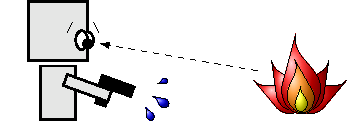
\includegraphics[scale=0.9]{robot_pompier}};
\node (bli) at (0,6.5) {};
\node (pomdp3) at (3.9,6) {\color{orange}{$s \in \mathcal{S}$}: \color{black}{\textbf{�tat du syst�me}}};
\node (t1) at (2,6) {};
\node (r1) at (-2.3,5.5) {};
\node (r11) at (1,4.5) {};
\draw[->,>=latex,color=orange!60,line width=1mm] (t1) to (r1);
\draw[->,>=latex,color=orange!60,line width=1mm] (t1) to (r11);
\node (pomdp4) at (5.8,4.45) {\color{blue!60}{$o \in \mathcal{O}$:} \color{black} \textbf{observations du syst�me}};
\node (t2) at (3.3,4.4) {};
\node (r2) at (-2.3,5.05) {};
\draw[->,>=latex,color=blue!40,line width=1mm] (t2) to[bend left] (r2);
\node (pomdp5) at (1.8,3) {\color{red}{$a \in \mathcal{A}$:} \color{black} \textbf{actions de l'agent}};
\node (t3) at (-0.3,3) {};
\node (r3) at (-2,4.2) {};
\draw[->,>=latex,color=red!50,line width=1mm] (t3) to (r3);
\node (pomdp6) at (-5.5,5.5) {\color{ggreen}{$b \in \mathbb{P}^{\mathcal{S}}$:} \color{black} }; %%% ORANGE?
\node (pomdp7) at (-5,5) {\color{black} \textbf{�tat de croyance} }; %%% ORANGE?
\node (pomdp6) at (-3.5,6) {\color{ggreen}{\Huge \textbf{?}}}; %%% ORANGE?
\end{tikzpicture}
\caption[Utilisation d'un PDMPO pour la mod�lisation du robot pompier]{
Utilisation d'un PDMPO pour la mod�lisation du robot pompier:
dans cet exemple, la mission du robot est la pr�vention des incendies.
L'�tat du syst�me $s�\in \mathcal{S}$ d�crit par exemple la position du robot, 
l'orientation du jet d'eau, la quantit� d'eau utilis�e,
la position du feu et son niveau sur une �chelle ``petit feu'' et ``feu important'', etc.
En utilisant une vision artificielle et des capteurs de chaleur,
le robot re�oit des \textbf{observations} $o \in \mathcal{O}$
qui sont les donn�es brutes ou trait�es provenant des capteurs:
la sortie d'un classifieur dont l'entr�e est une image de la sc�ne
(\textit{cf.} Figure \ref{observation_robot}), 
et qui renvoie le niveau ou la position du feu,
peut �tre mod�lis� par une observation.
Finallement, les \textbf{actions du robot} $a \in \mathcal{A}$ 
sont par exemple la mise en marche des moteurs
impactant la rotation des roues du robot, 
le d�bit de pompage,
l'orientation du jet d'eau ou des capteurs, etc.
%Uncertainty dynamics is described by conditional probability distributions:
La \textbf{fonction de r�compense} $r(s,a)$
d�cro�t avec le niveau de l'incendie.
Afin de ne pas gaspiller d'eau,
un co�t proportionnel � la quantit� d'eau
est soustrait � cette r�compense:
puisque une strat�gie optimale maximise la moyenne de la somme des r�compenses,
le but du robot est donc d'attaquer les incendies sans gaspiller d'eau.
Cette moyenne peut-�tre calcul�e � l'aide des probabilit�s d�crivant la dynamique stochastique du syst�me.
Les actions du robot $a \in \mathcal{A}$ ont un effet probabiliste sur le syst�me,
d�crit par la \textbf{fonction de transition} $\textbf{p} \paren{s' \sachant s,a}$: 
par exemple, l'activation des roues du moteur modifie la position du robot,
et la probabilit� sur chacune des positions suivantes possibles,
�tant donn� la position courante,
prend part � la d�finition du PDMPO.
Un autre exemple est l'action modifiant l'orientation du jet d'eau,
qui red�finit la probabilit� du nouveau niveau de feu �tant donn� l'�tat actuel du syst�me.
Les actions du robot $a \in \mathcal{A}$
et les �tats suivants $s' \in \mathcal{S}$ 
peuvent aussi impacter les observations des capteurs:
cette influence est d�finie par la \textbf{fonction d'observation} $\textbf{p} \paren{o' \sachant s',a}$: 
par exemple, l'orientation du capteur de vision peut modifier
la probabilit� de d�tection du feu, 
ou de l'�valuation de son intensit�, 
qui font partie des observations $o' \in \mathcal{O}$. 
Finalement, l'�tat de croyance est la distribution de probabilit� sur l'�tat courant du syst�me 
conditionnellement � l'ensemble des observations et actions successives depuis le d�but du processus:
c'est la meilleure estimation possible puisque le robot n'a acc�s qu'aux actions et observations
lors de l'ex�cution.}
\label{robot_pompier}
\end{figure}

Il a �t� montr� que de telles strat�gies markoviennes sont optimales
pour certain crit�res
tels que celui bas� sur la somme des r�compenses d�compt�es:
en effet, un crit�re bien connu mesurant 
les performances d'une strat�gie $d$
est l'esp�rance de la somme actualis�e des r�compenses: 
\begin{equation}
\label{criterion}
\mathbb{E} \croch{ \sum_{t=0}^{+ \infty} \gamma^t r(s_t,d_t) },
\end{equation}
o� $d_t=d(s_t) \in \mathcal{A}$ 
et $0<\gamma<1$ est un facteur d'actualisation
assurant la convergence de la somme.

L'hypoth�se que l'agent a une connaissance parfaite de l'�tat du syst�me
est assez forte:
en particulier, dans le cas des robots r�alisant des taches avec des capteurs conventionnels,
ces derniers sont souvent incapable de fournir au robot
toutes les caract�ristiques d'int�r�t pour la mission.
Ainsi, un mod�le plus flexible, 
\textit{i.e.} qui tient compte de \textit{l'observation partielle} du syst�me par l'agent, a �t� construit.
%%% ROBOT POMPIER FIN

%%% POMDP
En effet, les MDP Partiellement Observables 
(PDMPO) \cite{Smallwood_Sondik} 
ont une puissance de mod�lisation plus importante,
car ils peuvent repr�senter des situations 
dans lesquelles l'agent
ne conna�t pas directement l'�tat courant du syst�me:
ils mod�lisent de mani�re plus fine 
un agent ex�cutant des actions 
sous incertitude dans un environnement
partiellement observable. 

L'ensemble des �tats du syst�me $\mathcal{S}$,
l'ensemble des actions $\mathcal{A}$, 
la fonction de transition $\textbf{p} \paren{ s_{t+1} \sachant s_t,a_t}$ 
et la fonction de r�compense $r(s,a)$ 
restent les m�me que pour la d�finition des PDM.
Dans ce mod�le, puisque l'�tat courant du syst�me
$s \in \mathcal{S}$ 
ne peut pas �tre consid�r� comme une information accessible pour l'agent,
la connaissance de l'agent � propos de l'�tat du syst�me 
provient des observations $o \in \mathcal{O}$, 
o� $\mathcal{O}$ est un ensemble fini. 
%A full definition of this process 
%includes as well the set of 
%possible observations of the system, 
%$o \in \mathcal{O}$. 
La fonction d'observation 
$\textbf{p} \paren{ o_{t+1} \sachant s_{t+1},a_t }$
donne pour chaque action $a_t \in \mathcal{A}$
et �tat atteint $s_{t+1} \in \mathcal{S}$, 
la probabilit� sur les observations possibles $o_{t+1} \in \mathcal{O}$. 
Enfin, \textit{l'�tat de croyance initial} $b_0(s)$
d�finit la distribution de probabilit� \textit{a priori}  
sur l'�tat du syst�me.
Un exemple d'usage des PDMPO est illustr� 
dans la figure \ref{robot_pompier}.

R�soudre un POMDP consiste � calculer une strat�gie 
qui renvoie une action ad�quate � chaque �tape du processus, 
et d�pendente des observations re�ues et des actions s�lectionn�es
\textit{i.e.} de toutes les donn�es disponibles pour l'agent:
un crit�re pour la strat�gie peut aussi �tre
l'esp�rance de la somme actualis�e des r�compenses (\ref{criterion}).

%
% belief
%
La plupart des algorithmes raisonnent sur \textit{l'�tat de croyance},
d�fini comme la distribution de probabilit� sur l'�tat du syst�me
conditionnellement � toutes les observations du syst�me 
et les actions choisies par l'agent depuis le d�but du processus.
Cet �tat de croyance est mis � jour � chaque �tape de temps en utilisant la r�gle de Bayes,
l'action courante,
et la nouvelle observation.
\`A une �tape donn�e $t \in \mathbb{N}$, 
$b_t(s)$ est d�fini
comme la probabilit� que le $t^{i�me}$ �tat du syst�me soit 
$s \in \mathcal{S}$, connaissant les observations et actions pr�c�dentes,
ainsi que l'�tat de croyance initial $b_0$:
c'est une estimation de l'�tat du syst�me
qui utilise uniquement les donn�es disponibles
puisque l'�tat n'est pas directement observable.

Il peut �tre facilement calcul� de mani�re r�cursive avec la r�gle de Bayes: 
� l'�tape de temps $t$, 
si l'�tat de croyance est $b_t$, 
l'action choisie $a_t \in \mathcal{A}$ 
et la nouvelle observation 
$o_{t+1} \in \mathcal{O}$, 
l'�tat de croyance suivant
\begin{eqnarray}
\label{probBayesRule}
b_{t+1}(s')  \propto \textbf{p} \paren{ o_{t+1} \sachant s', a_t } \cdot \sum_{s \in \mathcal{S}} \textbf{p} \paren{s' \sachant s,a_t} \cdot b_t(s).
\end{eqnarray}
comme illustr� par le r�seau Bayesien de la figure \ref{BayesNetPOMDP}.
%
% BAYESNET
%
\begin{figure}\centering
\begin{tikzpicture}
%%%%%%%%%%%%%%%%%%%%%%%%%%%%%%%%%%%%%%%%%%%%%%%%%%%%%%%%%%%%%%
%vertex
\tikzstyle{vertex}=[circle,fill=black!40,minimum size=30pt,inner sep=0pt,draw=black,thick]
\tikzstyle{avertex}=[rectangle,fill=red! 60,minimum size=25pt,inner sep=0pt,draw=black,thick]
\definecolor{darkgreen}{rgb}{0.3,0.8,0.5}
\tikzstyle{overtex}=[circle,fill=blue!50,minimum size=30pt,inner sep=0pt,draw=black,thick]
%nodes
\node[vertex] (state1) at (0,1.8) {$S_t$};
\node[vertex] (state2) at (7,1.8) {$S_{t+1}$};
\node[overtex] (obs) at (13,0) {$O_{t+1}$};
\node[avertex] (action) at (2.5,0) {$a_t$};
%%bels
\node (bel1) at (1,2.5) {$b_t$};
\node (bel2) at (8.5,2.5) {$b_{t+1}$};
%probas
\node (trans) at (4.5,1.5) {$\textbf{p} \paren{ s_{t+1} \sachant s_t, a_t }$};
\node (observ) at (9.6,0.3) {$\textbf{p} \paren{ o_{t+1} \sachant s_{t+1}, a_t }$};
%%%%%%%%%%%%%%%%%%%%%%%%%%%%%%%%%%%%%%%%%%%%%%%%%%%%%%%%%%%%%%
%ARROWS
\draw[->,>=latex, thick] (state1) -- (state2);
\draw[->,>=latex, thick] (state2) -- (obs);
\draw[->,>=latex, thick] (action) -- (state2);
\draw[->,>=latex, thick] (action) -- (obs);
\end{tikzpicture}
\caption[R�seau Bayesien illustrant la mise � jour de l'�tat de croyance]{R�seau Bayesien illustrant la mise � jour de l'�tat de croyance: 
les �tats sont repr�sent�s par des ronds gris, 
l'action est repr�sent�es par le losange rouge,
et l'observation par le rond bleu.
La variable al�atoire $S_{t+1}$
repr�sentant l'�tat suivant $s_{t+1}$ 
d�pend de l'�tat courant $s_t$ 
et de l'action courante $a_t$.
La variable al�atoire $O_{t+1}$ 
r�pr�sentant l'observation suivante $o_{t+1}$ 
d�pend de l'�tat suivant $s_{t+1}$
et de l'action courante $a_t$.
L'�tat de croyance $b_{t}$ (resp. $b_{t+1}$)
est l'estimation probabiliste du l'�tat courant (resp. suivant) du syst�me, 
$s_t$ (resp. $s_{t+1}$).}
\label{BayesNetPOMDP}
\end{figure}%

Puisque les �tats de croyance successifs sont calcul�s avec les observations per�ues par l'agent,
ils sont consid�r�s visible par l'agent. 
%Moreover, it can be easily shown that
%the expected total reward can be rewritten 
%\begin{equation}
%\label{probCriterion}
%\mathbb{E} \croch{ \sum_{t=0}^{+ \infty} \gamma^t r(s_t,d_t) } = \mathbb{E} \croch{ \sum_{t=0}^{+ \infty} \gamma^t r(b_t,d_t) }, 
%\end{equation}
%defining $r(b_t,a) = \sum_s r(s,a) \cdot b_t(s)$ as the reward of belief $b_t$.
Notons $\mathbb{P}^{\mathcal{S}}$ 
l'ensemble continu des distributions de probabilit�
sur $\mathcal{S}$.
Une strat�gie optimale peut �tre cherch�e parmi
les fonction $d$ d�finies sur $\mathbb{P}^{\mathcal{S}}$ 
telles que les $d_t = d(b_t) \in \mathcal{A}$ successifs 
maximisent l'esp�rance des r�compenses (\ref{criterion}):
les d�cisions de l'agent sont bas�es sur l'�tat de croyance.

%
% POMDP ROBOTICS
%
Les PDMPO fournissent un cadre flexible pour la robotique autonome,
comme illustr� par l'exemple du robot pompier, \textit{cf.} figure \ref{robot_pompier}:
ils permettent de d�crire le syst�me regroupant le robot et son environnement,
ainsi que la mission du robot.
Ils sont fr�quemment utilis�s en robotique
\cite{PineauG05,OngShaoHsuWee-IJRR10,Marthi12,ChanelTL12,ChanelTL13}.
En effet, ils prennent en compte le fait que le robot ne re�oit que les donn�es des capteurs,
et doit estimer l'�tat du syst�me, qui lui est cach�,
en utilisant ces donn�es, appel�es alors observations,
afin de r�aliser sa mission.
Cependant, le mod�le PDMPO soul�ve quelques probl�mes,
en particulier dans le contexte robotique.

%
% HIGH COMPLEXITY
%
\section*{Probl�mes pratiques des PDMPO}
\subsection*{Complexit�}
R�soudre un PDMPO \textit{i.e.} 
calculer une strat�gie optimale,
est PSPACE-hard en horizon fini \cite{Papadimitriou1987} 
et m�me ind�cidable en horizon infini \cite{Madani1999UPP315149.315395}.
De plus, un espace exponentiel en la description du probl�me peut �tre requis
pour une sp�cification explicite d'une telle strat�gie.
Le travail \cite{Mundhenk2000CPP867838} 
est un bon r�sum� des l'analyses de complexit�
des PDMPO.

Cette forte complexit�
est tr�s bien connue des utilisateurs des PDMPO:
l'optimalit� ne peut �tre atteinte que pour des petits probl�mes,
ou bien des probl�mes tr�s structur�s.
Les approches classiques essaient de r�soudre ce probl�me
en utilisant la programmation dynamique
et des techniques de programmation lin�aire
\cite{Cassandra97incrementalpruning}.
Sinon, seules des solutions approch�es peuvent �tre calcul�es,
et donc la strat�gie n'a pas de garantie d'optimalit�.
Par exemple, les approches populaire
telles que les m�thodes bas�es sur les points,
\cite{Pineau_2003_4826,Kurniawati-RSS08,Smith2004HSV1036843.1036906}, 
celles bas�es sur des grilles \cite{Geffner98solvinglarge,Brafman97aheuristic,Bonet_newgrid-based}
ou bien les approches de Monte Carlo approaches \cite{NIPS2010_4031},
utilisent des calculs approch�s.

%
% VISION IN ROBOTICS
%
\begin{figure} \centering

\includegraphics[scale=0.75]{fig2}
\caption[Exemple d'une m�thode d'observation dans le contexte robotique]{
Exemple d'une m�thode d'observation dans le contexte robotique:
le robot, ici un drone, est �quipp� d'une cam�ra
et utilise un classifieur calcul� � partir d'une base de donn�es d'images
(comme NORB, \textit{cf.} figure \ref{NORB}).
Le classifieur est g�n�r� avant la mission (off-line)
avec une base de donn�es d'images
(\textit{cf.} partie droite de l'illustration), 
et la sortie du classifieur 
est utilis�e lors de la mission (online) 
comme une observation pour l'agent (\textit{cf.} la partie gauche).
Ici, les observations sont donc g�n�r�es par un algorithme de vision artificielle.}
\label{observation_robot}
\end{figure}
%
% VISION IN ROBOTICS END
%


%
% COMPUTER VISION
%
\subsection*{Impr�cision des Param�tres et Vision Artificielle}
Consid�rons maintenant des robots utilisant la perception visuelle,
et dont les observation proviennent d'algorithmes de vision
bas� sur de l'apprentissage statistique.
(\textit{cf.} figure \ref{observation_robot}).
Dans cette situation, le robot utilise un \textit{classifieur}
pour reconna�tre les objects dans les images:
le classifieur est cens� renvoyer le nom de l'objet
qui se trouve dans l'image,
et fait quelquefois des erreurs avec une faible probabilit�.
(\textit{i.e.} matrice de confusion de la figure \ref{confusion_matrix}).

Le classifieur est calcul� en utilisant une \textit{base de donn�e d'entra�nement} 
(comme NORB, \textit{cf.} figure \ref{NORB}, 
mis en ligne par les auteurs � l'adresse \url{http://www.cs.nyu.edu/~ylclab/data/norb-v1.0/}).
Un algorithme utilisant des descentes de gradient 
utilis� pour calculer le classifieur
en utilisant la base de donn�es d'images
est appel� R�seau Convolutionnel \cite{Lecun98gradient-basedlearning}.
Les figures (\ref{NORB}) et (\ref{confusion_matrix})
illustrent l'exemple d'un classifieur calcul� pour une mission dronique
dans laquelle les caract�ristiques d'int�r�t
(les �tat du syst�me)
sont li�es � la pr�sence (ou l'abscence)
d'animaux, voitures, humains, avions ou camions: 
le probl�me statistique du calcul d'un classifieur 
permettant de reconnaitre de tels objets dans les images
est appel� \textit{classification multi-classes}.

%%%
%%% NORB DATA SET
%%%

\newcounter{moncompteur} %define counter
\begin{figure} \centering
\begin{tikzpicture}
\node (notes) at (2.5cm,7cm) { 
base de donn�es d'images NORB: \color{blue} $(\mbox{image}_i,\mbox{�tiquette}_i)_{i=1}^N$
};

\def\names{{"bla","human","car","truck","truck","nothing","nothing","nothing","truck"}}%
\def\namess{{"bla","airplane","car","human","animal","car","human","animal","animal"}}%

\setcounter{moncompteur}{1}
	\coordinate (norb11) at (6.2cm,3.05cm); 
	\coordinate (norb12) at (14cm,3.05cm); 
	\coordinate (norb11lab) at (6.2cm,6.2cm); 
	\coordinate (norb12lab) at (14cm,6.2cm); 
	\coordinate (norb11lab2) at (6.2cm,1.9cm); 
	\coordinate (norb12lab2) at (14cm,1.9cm); 
	\foreach \y in {0.25,0.5,...,2} {
		\coordinate (weight) at (barycentric cs:norb11= \y,norb12=1-\y);
		\def\reptemp{photos/} %define string
		\appto\reptemp{\themoncompteur} %access the string of a counter
		\appto\reptemp{.png} % concatenate two trings
		\node (image) at (weight) {\includegraphics[scale=0.5]{\reptemp}};
		
		\coordinate (weight2) at (barycentric cs:norb11lab= \y,norb12lab=1-\y);
		\node[scale=0.7] (leslabels) at (weight2) {\pgfmathparse{\names[\themoncompteur]}\pgfmathresult};
		\coordinate (weight3) at (barycentric cs:norb11lab2= \y,norb12lab2=1-\y);
		\node[scale=0.7] (leslabels) at (weight3) {\pgfmathparse{\namess[\themoncompteur]}\pgfmathresult};

		\addtocounter{moncompteur}{1}
	}

	\coordinate (norb21) at (6.2cm,5cm); 
	\coordinate (norb22) at (14cm,5cm); 
	\foreach \y in {0.25,0.5,...,2} {
		\coordinate (weight) at (barycentric cs:norb21= \y,norb22=1-\y);
		\def\reptemp{photos/} %define string
		\appto\reptemp{\themoncompteur} %access the string of a counter
		\appto\reptemp{.png} % concatenate two trings
		\node (image) at (weight) {\includegraphics[scale=0.5]{\reptemp}};
		\addtocounter{moncompteur}{1}
	}

\end{tikzpicture}
\caption[Exemple de base de donn�e pour la vision artificielle]{Exemple de base de donn�e pour la vision artificielle: 
la base de donn�es d'images �tiquet�es NORB \cite{LeCun.2004},
destin�e � l'apprentissage statistique.
La taille de NORB est sup�rieure � $3.10^5$,
et les images de cette base de donn�es repr�sentent des objets de ces $5$ classes:
``animal'', ``car'', ``human'', ``nothing'', ``plane'' et ``truck''.
Chaque �l�ment d'une base de donn�e d'images est compos� d'une image (par exemple une image montrant une voiture)
et une �tiquette correspondant � la classe de l'objet repr�sent� par l'image 
(dans l'exemple pr�c�dent, l'�tiquette est ``car'').
Cette base de donn�es peut �tre utilis�e afin de calculer un classifieur par apprentissage supervis�.
Dans le but de discerner les positions des cibles,
une image est �tiquet�e avec le nom de l'objet qui est au centre
(``nothing'' si il n'y a rien au centre de l'image).}
\label{NORB}
\end{figure}
%%%%%
%%%%% NORB DATASET END
%%%%%
%
% IMPRECISION OBSERVATION
%
Puisque le classifieur est appris � partir d'une base de donn�es d'images,
son comportement, et donc ses performances,
(\textit{i.e.} sa fr�quence de bonne pr�dictions) 
est in�vitablement d�pendent de la base de donn�es.
C'est un probl�me si la variabilit� de la base de donn�e
est trop faible:
dans ce cas, le comportement probabiliste du classifieur
sera d�pendent de ces images en particulier
et le syst�me robotique aura des mauvaises capacit�s d'observations
lorsque la mission implique des images trop diff�rentes de celles pr�sentes
dans la base de donn�es.

Certaines bases de donn�es � grande variabilit� existent
(par exemple NORB, figure \ref{NORB}, bien que la variabilit� pourrait �tre id�alement sup�rieure):
notons cependant qu'avec ces bases de donn�es,
la performace de vision est r�duite,
ou bien, au moins, de bonne performances
sont difficilement atteignables

Une matrice de confusion peut �tre calcul�e (\textit{cf.} figure \ref{confusion_matrix})
en utilisant une telle base de donn�es �tiquet�es,
qui n'est pas utilis�e pour l'entra�nement,
et qui est appel�e \textit{base de donn�es de test}:
la fr�quence des observations peut �tre d�duit de cette matrice,
en normalisant les lignes en distributions de probabilit�.
Une ligne correspond � un objet de la sc�ne
et les probabilit�s de cette ligne sont les probabilit� d'observation,
\textit{i.e.} chaque valeur de probabilit� est la fr�quence avec laquelle
le classifieur renvoie le nome de l'objet de la colonne correspondante.
Ces probabilit�s peuvent �tre utilis�es pour d�finir la fonction d'observation
$\textbf{p} \paren{o' \sachant s',a}$ introduite au-dessus.
Cette approche soul�ve le probl�me de la repr�sentativit�
de la base de donn�es pour la mission voulue.
Si la base de donn�e de test n'est pas repr�sentative,
ces probabilit�s d'observation risque de ne pas �tre fiables,
et le PDMPO mal d�fini:
cependant, comme montr� par l'�quation (\ref{probBayesRule})
la mise � jour de l'�tat de croyance n�cessite la connaissance parfaite
de la fonction d'observation.

Finalement, si les bases de donn�es consid�r�e sont �tiquet�es plus pr�cis�ment,
(comme NORB, qui inclut des informations telles que la luminosit�, ou l'�chelle de l'objet),
nous pouvons imaginer que les probabilit�s d'observation calcul�es (� partir de la matrice de confusion)
serait plus fiable, ou la performance de vision am�lior�e
(puisque la s�paration demand�e au classifieur 
est plus simple avec cette pr�cision).
Cependant, comme plus d'observations ou d'�tats sont impliqu�es,
et le POMDP est plus dur � r�soudre.

En guise de conclusion, l'utilisation du mod�le PDMPO fait l'hypoth�se
que les distributions de probabilit� r�gissant le probl�me doivent �tre toutes connues parfaitement:
malheureusement ces fr�quences ne sont pas connue pr�cis�ment en pratique.
L'impr�cision � propos de ces probabilit�s,
par exemple l'impr�cision associ�e au comportement des sorties
des algorithmes de vision artificielle,
lorsque les images utilis�es sont celles de la mission d'int�r�t,
doit �tre prise en compte pour rendre le robot autonome en toute circonstances.
En g�n�ral, le calcul des distributions de probabilit� d'un PDMPO n�cessite
assez de tests pour chaque paire �tat-action, ce qui est dur � effectuer en pratique.

\begin{figure}[b!] \centering
\begin{tabular}{c|c|c|c|c|c!{\vrule width 2pt}c!{\vrule width 2pt}c}%!{\vrule width 2pt}}
animal & human & plane & truck & car & nothing \\ \specialrule{.2em}{.0em}{.0em}  
$3688$ & $575$ & $256$ & $48$ & $144$ & $149$ &   animal & $75.885\%$ \\ \specialrule{.05em}{.0em}{.0em}  
$97$ & $4180$ & $81$ & $20$ & $225$ & $257$ & human & $86.008\%$ \\  \specialrule{.05em}{.0em}{.0em}  
$292$ & $136$ & $3906$ & $237$ & $202$ & $87$ & plane & $80.370\%$ \\  \specialrule{.05em}{.0em}{.0em}  
$95$ & $1$ & $44$ & $4073$ & $514$ & $133$ & truck & $83.807\%$  \\  \specialrule{.05em}{.0em}{.0em}  
$129$ & $3$ & $130$ & $1283$ & $3283$ & $32$ &  car & $67.551\%$ \\  \specialrule{.05em}{.0em}{.0em}  
$154$ & $283$ & $36$ & $63$ & $61$ & $4263$ & nothing & $87.716\%$  \\ %\specialrule{.2em}{.0em}{.0em}  
\end{tabular}
\caption[Exemple de matrice de confusion illustrant les performances d'un classifieur multi-classes]{
Exemple d'une matrice de confusion pour la classification multi-classe:
cette matrice est calcul�e avec une base de donn�e de tests,
diff�rente de la base de donn�es d'apprentissage.
Chaqye ligne ne consid�re que les images d'un certain objet,
et les nombres repr�sentent les r�ponses du classifieur:
par exemple, $3688$ images d'animaux sont bien reconnus, 
mais $575$ sont confondus avec un humain.
La moyenne de r�ponses correctes pour cet objet et de $80.223\%$.
L'environnement Torch7 \cite{Collobert_NIPSWORKSHOP_2011}
a �t� utilis� pour obtenir un classifieur, 
et pour calculer cette matrice � partir de ce dernier
et de la base de donn�e de test.}
\label{confusion_matrix}
\end{figure}


%
% IMPRECISION POMDP WORKS
%
Quelques variations du cadre PDMPO
a �t� constuit dans le but de prendre en compte
l'impr�cision sur les distributions de probabilit� du mod�le,
aussi appel� \textit{l'impr�cision des param�tres}.
\subsubsection{Travaux Tenant Compte de l'Impr�cision des Param�tres} 
Ici, les fonctions de transition et d'observation,
\textit{i.e.} $\textbf{p} \paren{ s' \sachant s,a }$ 
et $\textbf{p} \paren{ o' \sachant s',a }$,
$\forall (s,s',o',a) \in \mathcal{S}^2 \times \mathcal{O} \times \mathcal{A}$,
sont appel�s \textit{param�tres} du PDMPO, 
ou aussi les \textit{param�tres} du mod�le. 
A notre connaissance,
le premier mod�le construit dans le but de g�rer l'impr�cision
des param�tres est nomm� PDMPOPI, 
pour \textit{PDMPD � param�tres impr�cis} \cite{Itoh2007453}. 
Dans ce travail, chacun des param�tres du PDMPO
est remplac� par un ensemble de param�tres possibles.
Dans ce travail, une \textit{croyance du second ordre}
est introduite: elle est d�finie comme �tant
la distribution de probabilit� sur les param�tres du mod�les.

Un autre travail, appel� \textit{PDMPO � Param�tres Born�s} 
(PDMPOPB) \cite{NiYaLiaZhi},
traite aussi de l'impr�cision des param�tres:
dans ce travail, l'impr�cision sur chaque param�tre
est d�crit � l'aide d'une borde sup�rieure et inf�rieure
sur les distributions possibles.
Aucune croyance du second ordre n'est introduite ici.
Cependant, r�soudre un PDMPOPB est similaire, dans l'esprit, 
� la r�solution des PDMPOPI \cite{Itoh2007453}:
la flexibilit� amen�e par l'impr�cision de param�tres
est utilis�e pour rendre les calculs les plus faciles possible,
et le crit�re utilis� n'est pas explicite.
Le probl�me majeur de ces approches (PDMPOPI et PDMPOPB)
est que l'impr�cision des param�tres n'est pas g�r� dans un but de robustesse,
comme une approche pessimiste (pire cas),
mais dans un but de simplification. 

Un travail plus r�cent traite le probl�me de mani�re pessimiste 
et est donc appel� \textit{PDMPO robuste} \cite{Osogami15}.
Inspir� par le travail correspondant dans le cas compl�tement observable
(appel� \textit{PDM uncertain} \cite{NE05}),
ce travail utilise le crit�re dit \textit{maximin},
ou du \textit{pire cas},
qui vient de la \textit{Th�orie des jeux}: 
dans ce cadre, une strat�gie optimale
maximise le plus petit crit�re
parmi ceux induits par chaque param�tre possible.
Si l'impr�cision des param�tres n'est pas stationnaire,
\textit{i.e.} peut changer � chaque �tape de temps,
la strat�gie optimale associ�e (au sens du maximin)
peut �tre facilement calcul� en utilisant la
\textit{Programmation Dynamique} \cite{bellman54}.
Cependant, lorsque l'impr�cision des param�tres est stationnaire,
les choses se compliquent:
les calculs propos�s m�nent � une approximation de la strat�gie optimale,
puisque le crit�re utilis� est une borne inf�rieur
du crit�re d�sir�.
Pourtant, une hypoth�se stationnaire pour l'impr�cision
des param�tres semble mieux adapt�e lorsque le PDMPO est stationnaire.

Bien que l'utilisation d'ensembles de distributions de probabilit� 
rend le mod�le plus adapt� � la r�alit� du probl�me
(les param�tres sont impr�cis en pratique),
les prendre en compte augmente violemment 
la complexit� du calcul d'une politique optimale
(par exemple, lors de l'utilisation du crit�re maximin).
Comme expliqu� pr�c�demment,
r�soudre un PDMPO est d�j� une t�che tr�s ardue,
donc l'utilisation d'un cadre menant � des calculs plus complexes
ne semble pas �tre une approche satisfaisante.
%and optimization may require linear programs 
%As discussed during this thesis 
%(for instance see Section \ref{section_expe_PPUDD} of Chapter \ref{chap_symb}),
En effet, mod�liser le probl�me de mani�re trop fine
m�ne � l'utilisation de nombreuse approximations
dans les calculs en pratique,
sans r�el contr�le ou estimation de ces approximations
comme dans le cas des PDMPOPI et des PDMPOPB.
Il est peut-�tre plus judicieux de commencer avec un mod�le plus simple
qui peut �tre r�solu plus facilement en pratique.

Un autre probl�me pratique du mod�le PDMPO
peut aussi �tre mentionn�: 
cela concerne la d�finition de l'�tat de croyance
durant les premi�res �tapes du processus,
et plus g�n�ralement, la mani�re avec laquelle
la connaissance de l'agent est repr�sent�e.
%%
%%  FULL IGNORANCE/ KNOWLEDGE OF THE AGENT
%%
\subsection*{Mod�liser l'Ignorance de l'Agent}
L'�tat de croyance initial $b_0$, 
ou distribution de probabilit� \textit{a priori} 
sur l'�tat du syst�me, prends part dans la d�finition
du PDMPO. 
\'Etant donn� un �tat du syst�me $s \in \mathcal{S}$, 
$b_0(s)$ est la fr�quence de l'�v�nement ``l'�tat initial est $s$''.
Cette quantit� peut �tre dure � calculer rigoureusement,
surtout lorsque le nombre d'exp�riences pass�es est limit�: 
cette raison a d�j� �t� invoqu�e au-dessus, 
menant � l'impr�cision des fonctions de transition et d'observation.

Consid�rons l'exemple d'un robot qui est pour la premi�re fois dans une salle
dont la position de la sortie est inconnue 
(�tat de croyance initial)
et qui doit trouver la sortie et l'atteindre.
En pratique, aucune exp�rience ne peut �tre
r�p�t�e dans le but d'extraire une fr�quence de position
pour cette sortie.
Dans ce genre de situation, l'incertitude n'est pas due
� un �v�nement al�atoire, mais � un manque de connaissance:
aucun �tat de croyance initial fr�quentiste ne peut �tre utilis� pour d�finir le mod�le.

L'agent peut aussi croire fortement
que la sortie est positionn�e dans un mur,
comme dans la plupart des salles,
mais il attribue quand-m�me une tr�s petite probabilit� $p_{\epsilon}$ 
au fait que la sortie peut �tre un escalier au plein milieu de la salle.
M�me si il est tr�s peu probable que ce soit le cas,
cette seconde option doit �tre prise en compte
dans l'�tat de croyance,
sinon la r�gle de Bayes (\textit{cf.} �quation \ref{probBayesRule}) 
ne peut pas �tre le mettre � jour correctement
si la sortie est vraiment au centre de la pi�ce.
Quantifier $p_{\epsilon}$ sans exp�rience pass�e
n'est pas une chose facile du tout,
et ne se repose sur aucune justification rationnelle,
mais peut impacter fortement la strat�gie de l'agent.

L'�tat initial du syst�me peut �tre d�lib�r�ment
d�fini comme �tant inconnu, avec strictement aucune
information probabiliste:
consid�rons une mission robotique
pour laquelle une partie de l'�tat du syst�me,
d�crivant un fait que le robot est cens�
d�couvrir par lui-m�me, est
initialement compl�tement inconnu.
Dans un contexte d'exploration robotique,
la position ou la nature d'une cible,
ou encore la position initiale du robot,
peut �tre d�fini comme �tant absent de la connaissance de l'agent.
Les approches classiques initialisent l'�tat de croyance
par une distribution de probabilit� uniforme.
(\textit{i.e.} sur toutes les position possible du robot/cible, 
ou sur toutes les natures de cible possibles), 
mais cette r�ponse provient de l'interpr�tation subjective
des probabilit�s \cite{de1974theory,Dubois96representingpartial}.
En effet, les probabilit�s sont les m�me
puisque aucun �v�nement n'est plus plausible qu'un autre:
cela correspond � des paris �gaux.
Cependant, les mises � jour de l'�tat de croyance (\textit{cf.} �quation \ref{probBayesRule}) 
m�ne fatalement � un m�lange de probabilit�s fr�quentistes, \textit{i.e.}
les fonction de transition et observation,
avec cet �tat de croyance initial qui est une distribution de probabilit� subjective:
cela n'a pas toujours de sens, et dans tous les cas cette approche est douteuse.
Ainsi, l'utilisation des PDMPO dans ces contextes fait face � la difficult� de repr�senter l'ignorance de l'agent.


%it may make the  actually the real  the POMDP is in practice, a belief state may have an high entropy
%not because of the imprecision of the parameters, 
%may be not related to the agent's lack of knowledge in the probabilistic about the ,
%but rather to the 
%(fully known) 
%variance of the system state:
%hence the agent does not know 
%which is the actual system state 
%since its  is far from being deterministic,
%but it may perfectly know how the state behaves,
%and then nothing can be improved concerning its knowledge.

%and knowledge of the agent CARO \\

%
% WHAT WE WOULD LIKE TO DO
%
\section*{Probl�me G�n�ral}
Les sections pr�c�dentes ont pr�sent� certain probl�mes rencontr�s en pratique
lors de l'utilisation des PDMPO pour calculer des strat�gies,
en particulier dans le cadre robotique.
La tr�s grande complexit�
du calcul d'une strat�gie optimale
est un premier probl�me:
les missions robotiques 
sont souvent des probl�mes � grandes dimensions,
dont le calcul d'une strat�gie suffisamment proche de l'optimal
est impossible, 
du fait d'un trop grand temps de calcul
ou d'un manque de m�moire.
Ensuite, il a �t� mis en �vidence
que les distributions de probabilit�
d�finissant le PDMPO 
ne sont pas toujours connues pr�cis�ment:
par exemple, la fonction d'observation
peut �tre difficile � d�finir 
lorsque les observations proviennent
d'un algorithme de vision artificielle complexe.
Enfin, le probl�me de la gestion de la connaissance et de l'ignorance de l'agent
a �t� discut�: il n'y a pas de r�ponse formelle
concernant la mani�re de repr�senter 
le manque de connaissance initial de l'agent
� propos du monde dans lequel il �volue.
La difficult� vient du fait que
les PDMPO classiques (probabilistes)
autorisent uniquement l'usage de distribution de probabilit� fr�quentiste,
alors qu'un autre outil math�matique semble n�cessaire.

Ces probl�mes forment le point de d�part de ce travail.
En effet, ce dernier consiste � contribuer
au probl�me du calcul d'une strat�gie
pour des domaines partiellement observables.
Les strat�gies calcul�es
doivent permettre au robot
de remplir sa mission
aussi bien que possible,
d�s la premi�re ex�cution
\textit{i.e.} le calcul de strat�gie 
est op�r� avant toute r�elle ex�cution
de la mission. 

Le chalenge g�n�ral guidant ce travail
est de proc�der aux calculs de strat�gies
en utilisant seulement les donn�es et les connaissances
vraiment disponibles en pratique,
au lieu d'utiliser les PDMPO classiques,
tr�s complexes et difficiles � d�finir.
En d'autre mots, cela revient � pr�ter attention
aux probl�mes soulev�s au-dessus:
la complexit� de calcul, l'impr�cision du mod�le,
et la gestion de la m�connaissance de l'agent. 
Comme expliqu� par la suite, la th�orie des possibilit�s qualitatives \cite{Dubois95possibilitytheory}
semble r�pondre aux probl�mes soulev�s.

\section*{Une Th�orie Qualitative}
Cette th�orie est g�n�ralement
introduite en d�finissant une
�chelle qualitative $\mathcal{L}$,
qui peut �tre d�finie par 
$\set{0,\frac{1}{k}, \frac{2}{k}, \ldots,1 }$, avec $k>1$,
ou tout autre ensemble fini totalement ordonn�.
Les valeurs de cette �chelle
ne sont pas importantes 
car elle servent seulement 
� mat�rialiser un ordre:
nous utilisons donc
le terme de \textit{degr� de possibilit�}
afin d'expliciter cette remarque.
Le plus petit �l�ment de l'�chelle qualitative est not� $0$,
et le plus grand, $1$.
La section suivante clarifie pourquoi
l'utilisation de ce cadre qualitatif 
est b�n�fique en terme de complexit�
et de mod�lisation.

Notons tout d'abord les similarit�s entre
la th�orie des probabilit�s et des possibilit�s:
une distribution de possibilit� sur $\mathcal{S}$ 
est une fonction $\pi: \mathcal{S} \rightarrow \mathcal{L}$
telle que $\max_{s \in \mathcal{S}} \pi(s) = 1$.
De plus, l'op�rateur $\min$ est utilis� pour calculer 
une distribution de possibilit� jointe 
$\pi(s,o)$, $\forall (s,o) \in \mathcal{S} \times \mathcal{O}$
� partir d'une distribution marginale $\pi(s)$, $\forall s \in \mathcal{S}$
et d'une distribution conditionnelle $\pi \paren{ o \sachant s }$, $\forall (o,s) \in \mathcal{S} \times \mathcal{O}$:
$\pi(s,o) = \min \set{ \pi (s), \pi \paren{ o \sachant s }  }$.
Ainsi, la th�orie des possibilit�s peut donc s'apprivoiser 
en rempla�ant l'op�rateur $+$ de la th�orie des probabilit�s
par l'op�rateur $\max$, et l'op�rateur $\times$ par $\min$.

%%% PIPOMDP
\subsection*{PDMPO Qualitatifs Possibilistes}
Une alternative possibiliste qualitative du mod�le PDMPO 
a �t� propos� dans \cite{Sabbadin1999pipomdp}:
ce mod�le s'appelle PDMPO qualitatif possibiliste,
et est not� $\pi$-PDMPO. 
Un $\pi$-PDMPO est simplement un PDMPO
avec des distributions possibilistes qualitatives comme param�tres,
au lieu de distributions de probabilit�s.
Comme les $\pi$-PDMPO sont qualitatifs,
l'homogue de la fonction de r�compense,
appel�e \textit{fonction de pr�f�rence},
est aussi qualitative:
en effet, la fonction de pr�f�rence 
est � valeurs dans l'�chelle possibiliste qualitative finie $\mathcal{L}$,
et donc n'est pas additive.

%%%% COMPLEXITY
L'une des propri�t�s les plus int�ressantes
des $\pi$-PDMPO est la simplification du calcul de la strat�gie.
En effet, les algorithmes propos�s
pour r�soudre les PDMPO probabilistes 
sont souvent bas�s sur l'ensemble des �tats de croyance
appel� \textit{espace des croyances}.
L'espace des croyances est infini dans le cas g�n�ral:
chaque �tape de temps m�ne � une nombre fini d'�tats de croyance suivants,
donc cet espace est d�nombrable.
Dans le but d'obtenir des propri�t�s utiles
et des moyens de calculer un strat�gie,
l'ensemble de toutes les distributions de probabilit�
sur l'espace d'�tat $\mathcal{S}$ est souvent consid�r�, 
\textit{i.e.} le simplex continu
$\mathbb{P}^{\mathcal{S}} 
= \set{ \textbf{p}:\mathcal{S} \rightarrow [0,1] \sachant \sum_{s \in \mathcal{S}} \textbf{p}(s) 
= 1, \mbox{ and } \textbf{p}(s)\geqslant 0, \forall s \in \mathcal{S} }$.
La taille infinie de l'espace des croyances
explique en partie
pourquoi les PDMPO probabilistes
sont vraiment difficiles � r�soudre.
Au contraire, les $\pi$-PDMPO ont un espace de croyances fini.
En effet, le nombre de distributions de possibilit�s qualitatives
sur les �tats du syst�me $\mathcal{S}$
est inf�rieur � $\mathcal{L}^{\# \mathcal{L}}$,
puisque l'�chelle qualitative $\mathcal{L}$ est finie.
La version compl�tement observable
d'un $\pi$-PDMPO est appel� $\pi$-PDM:
comme expliqu� dans la section \ref{section_piPOMDP} du chapitre \ref{chap_SOTA}, 
tout $\pi$-PDMPO se r�duit � un $\pi$-MDP 
dont l'espace d'�tat est l'ensemble des �tats de croyance possibilistes qualitatifs,
et dont la taille est exponentielle en fonction du nombre d'�tats du syst�me.
Dans les travaux \cite{abs-1202-3718,Garcia20081018,Sabbadin1999pipomdp}, 
il est montr� que
la complexit� d'un $\pi$-PDM
est plus faible que la complexit� d'un MDP probabiliste, 
qui est polynomiale \cite{Papadimitriou1987}:
la complexit� d'un $\pi$-PDMPO est akirs
au pire exponentiel en la description du probl�me,
tandis qu'un PDMPO probabiliste peut �tre ind�cidable \cite{Madani1999UPP315149.315395}.
%The approach of using a $\pi$-POMDP 
%instead of a probabilistic POMDP
%in order to simplify the resolution, 
%can be compared to 


%%% IMPRECISION MODELISATION
En plus de la simplification des calculs,
le $\pi$-PDMPO peut �tre vraiment int�ressant
pour nos probl�mes de mod�lisation. 
En effet, dans le cas d'un robot 
utilisant un algorithme de vision artificielle
(\textit{cf.} figure \ref{observation_robot}),
nous avons pr�c�demment mis en �vidence la difficult�
pour d�finir rigoureusement 
les fonction d'observation probabilistes:
les probabilit�s 
des r�ponses
des algorithmes de vision
dans le contexte d'une mission robotique
sont mal connus et difficiles � d�finir en pratique.
Trouver des estimations qualitatives
de ses performances de reconnaissance
est plus facile:
le mod�le $\pi$-PDMPO
ne requiert que des donn�es qualitatives, 
donc il permet de construire un mod�le
sans l'utilisation d'informations 
diff�rentes 
de celles vraiment disponibles.
Par exemple, la matrice de confusion 
de la figure \ref{confusion_matrix}
peut mener � une fonction d'observation
qualitative possibiliste
qui ne tient compte uniquement 
de la mani�re dont les fr�quences
de r�ponses sont class�es:
en pr�sence d'un humain (\textit{i.e.} deuxi�me ligne),
la r�ponse la plus fr�quente est ``human'',
la deuxi�me r�ponse est ``nothing'',
la troisi�me est ``car'', etc.
Donc, la distribution de possibilit� correspondante
est telle que,
conditionnellement � la pr�sence d'un humain, 
le degr� de possibilit� de la r�ponse ``human''
est plus grand que le degr� de possibilit� de la r�ponse ``nothing'',
qui est plus grand que le degr� de possibilit�
de la r�ponse ``car'', etc.
Au lieu d'attribuer des fr�quences
qui ne sont pas vraiment
fiable en pratique,
le mod�le possibiliste qualitatif
exprime naturellement ces impr�cisions
� propos du problem.

%%%IGNORANCE
Enfin, notons que la distribution de possibilit� 
constante, dont les degr�s sont tous �gaux � $1$
(�l�ment maximal de $\mathcal{L}$),
repr�sente l'ignorance totale:
cette distribution peut �tre utilis� 
pour d�finir l'�tat de croyance initial
lorsqu'il doit repr�senter
un agent qui ignore initialement
une situation donn�e.
Donc, le mod�le $\pi$-PDMPO
permet une mod�lisation formelle du manque de connaissance de l'agent. 

%%CORRESPONDS TO OUR ISSUES 
L'utilisation de la th�orie de possibilit�s qualitatives \cite{DuboisPS01}
est donc �tudi� dans ce travail,
puisqu'il semble �tre capable
d'� la fois simplifier un PDMPO,
et de mod�liser l'impr�cision des param�tres
et l'ignorance associ�es aux missions robotiques.
Ce cadre, en effet, simplifie les calculs,
est capable de repr�senter le probl�me avec seulement les donn�es disponibles,
et mod�lise le manque de connaissance:
donc cette th�orie offre ses solutions aux
trois probl�mes mis en �vidence pr�c�demment.
Cependent, notons qu'un cadre qualitatif
ne permet pas de manipuler de l'information fr�quentiste.

%%%NOT WIDELY STUDIED
A notre connaissance,
une �tude plut�t limit�e du mod�le $\pi$-PDMPO existe dans la litt�rature jusqu'� aujourd'hui:
en fait, le travail \cite{Sabbadin1999pipomdp}
semble �tre le seul, proposant
� la fois une d�finition des $\pi$-PDMPO 
et un exemple jouet pour illustrer ce mod�le.
La version compl�tement observable ($\pi$-PDM)
a g�n�r� plus de travaux \cite{Sabbadin2001287,Sabbadi00,LIP61498}.

\section*{Description de notre �tude}
% Le sujet de la th�se
Cette th�se contribue � d�terminer
dans quelle mesure la th�rie de possibilit�s qualitatives
peut contribuer � la \textit{planification dans l'incertain dans des domaines partiellement observables}, 
et plus g�n�ralement � la gestion s�quentielle de l'incertitude, 
en termes de simplification des calculs et de mod�lisation. 
Elle pr�sente de r�centes contributions
dans l'utilisation de cette th�orie pour la planification dans l'incertain
et la repr�sentation des connaissances,
avec une utilisation quasi syst�matique des mod�les graphiques 
\cite{Koller2009PGM1795555,Be2002.7,Borgelt02graphicalmodels}.

La fin de cette introduction 
d�crit la structure de cette cette th�se.
En effet, chacune des sections suivantes
correspond � un chapitre de notre travaille,
et d�taille son contenu.

%%%% SOTA
\subsection*{\'Etat de l'Art}
Les PDMPO qualitatifs et possibilistes 
constituent l'objet central de cette th�se:
le \emph{premier chapitre} est consacr� � ce mod�le.
Une pr�sentation rapide de la th�orie des possibilit�s qualitatives
est suivie de la pr�sentation du mod�le enti�rement observable ($\pi$-PDM),
puis du mod�le partiellement observable ($\pi$-PDMPO).
Comme not� pr�c�demment, � notre connaissance,
seulement un article de dix pages a d�j� trait� des $\pi$-POMDPs.

%%% CHAP1
\subsection*{Mises \`a jour naturelles du mod�le possibiliste qualitatif}
Le \emph{deuxi�me chapitre} propose quelques extensions
au travail \cite{Sabbadin1999pipomdp}.
Tout d'abord, est construite une version possibiliste qualitative
des PDM � observabilit� mixte \cite{OngShaoHsuWee-IJRR10,AraThoBufCha-ICTAI10}
dans lesquels quelques variables d'�tat sont compl�tement observables. 
Elle est appel�e $\pi$-PDMMO et g�n�ralise � la fois les $\pi$-PDM et les $\pi$-PDMPO.
Cette contribution r�duit consid�rablement 
la complexit� de r�solution des $\pi$-POMDPs, 
en manipulant de mani�re plus fine l'information des environnements
dont certaines variables sont compl�tement observables.
Par exemple, le niveau de batterie d'un robot peut �tre consid�r� comme
une information directement observable
pour la prise de d�cision, menant � des calculs plus simples.
Plus g�n�ralement, l'existence de variables visibles est tr�s courant 
en robotique \cite{OngShaoHsuWee-IJRR10}.

Ensuite, un crit�re qualitatif est propos�
pour pouvoir traiter des missions 
dont la dur�e n'est pas connue � l'avance:
l'algorithme faisant le calcul de la strat�gie optimale 
associ�e est alors pr�sent�.
Cet algorithme est utilis� pour calculer une strat�gie
pour une mission de reconnaissance de cible:
les r�sultats experimentaux comparent
les ex�cutions utilisant cette strat�gie
� celles utilisant la strat�gie d'un algorithme pour PDMPO probabiliste,
dans des situations o� la dynamique probabiliste des observations
n'est en fait mal d�finie.

Notons que ces r�sultats exp�rimentaux 
constituent, � notre connaissance, 
la premi�re utilisation du cadre $\pi$-PDMPO.
Ils mettent aussi en �vidence que l'�tat de croyance possibiliste qualitatif
a un comportement int�ressant, 
dans certaines situations d�taill�es par la suite.
Les principale contributions de ce chapitre
ont �t� publi�s dans \cite{Drougard13}.
Il est soulign� que les r�sultats exp�rimentaux
n'auraient pas pu �tre effectu�s
sans les deux premi�res contributions,
qui permettent de ne pas fixer un horizon arbitraire
et d'all�ger les calculs.

Cependant, ces contributions ne sont pas suffisantes
pour atteindre un temps de calcul comp�titif,
ou pour pouvoir traiter des probl�mes robotiques r�els:
l'orientation du second chapitre est dict�e par cette remarque.

%%% CHAP2
\subsection*{Mod�les factoris�s et algorithmes symboliques}

%% INTRO
Les probl�mes robotiques trait�s dans le chapitre pr�c�dent
sont assez petits pour permettre � l'algorithme propos�
de calculer une strat�gie
en un temps raisonnable.
Les contributions du \emph{troisi�me chapitre}
permettent la r�solution de probl�mes structur�s de planification
plus importants.

%% PPUDD and factored models
La premi�re partie de ce chapitre
se propose d'introduire
les \textit{$\pi$-PDMOM} factoris�s:
il sont d�finis par des hypoth�ses d'ind�pendance suppl�mentaires.
Les grands probl�mes de planification 
satisfaisant ces hypoth�ses 
peuvent �tre r�solus plus facilement:
inspir� par l'algorithme pour PDM probabilistes, 
SPUDD \cite{Hoey99spuddstochastic},
nous avons con�u un algorithme nomm� PPUDD
pour r�soudre les $\pi$-PDMOMs factoris�s 
en utilisant des \textit{arbres de d�cision alg�briques} (ADD).
L'intuition motivant cette contribution,
est que le calcul entre ADDs 
est moins co�teux en temps et en m�moire
dans le cadre qualitatif possibiliste %%%
que dans le cadre probabiliste:
les op�rations qualitatives
devraient mener � des ADDs plus petits
puisque la somme et le produit
sont remplac�s par les op�rateurs $\min$ et $\max$.
Ces derniers produisent des ADDs
avec potentiellement moins de feuilles,
car ils ne cr�ent pas de nouvelles valeurs.

%% belief factorization
Les hypoth�ses d'ind�pendance d�finissant
le mod�le $\pi$-PDMOM factoris� 
concerne les variables 
repr�sentant les croyances successives.
De plus, les variables d�finissant un
$\pi$-PDMOM sont celles repr�sentant
les �tats du syst�me et les observations.
C'est pourquoi la section qui suit dans ce chapitre
propose des conditions suffisantes
sur les variables d'�tat et d'observation
menant aux ind�pendances d�sir�es
entre les variables de croyances.
Un exemple robotique est utilis� en guise
d'illustration de ces conditions.
Puisque les preuves utilisent le concept
graphique appel� \textit{$d$-S�paration} \cite{pearl88},
ces conditions m�nent aussi � l'ind�pendance des 
variables de croyance dans le cadre des
PDMOM probabilistes.
 
%% first tests, larger robotic missions  
Les performances de notre solver PPUDD
sont ensuite compar�es � ceux des homologues probabilistes,
en termes de temps de calcul
et avec quelques crit�res mesurant 
la r�ussite de la mission.
Enfin, la derni�re partie de ce chapitre
d�crit les r�sultats de PPUDD
lors de la comp�tition internationale
de planification probabiliste\footnote{\url{https://cs.uwaterloo.ca/~mgrzes/IPPC_2014/}}.
Nous avons particip� � la comp�tition
dans le but de tester les performances de l'algorithme
contre celles des algorithmes probabilistes,
en terme d'esp�rances de la somme des r�compenses,
sur de nombreux probl�mes de planification.

Certaines contributions de ce chapitre
ont �t� publi�es dans \cite{DrougardTFD14}.
Les nombreux probl�mes de planification de la comp�tition
mettent aussi en �vidence 
quelques probl�mes li�s � notre algorithme,
lorsqu'il est utilis� pour approximer
le calcul d'une strat�gie
pour un probl�me probabiliste
dans le but de b�n�ficier de
calculs qualitatifs
qui sont plus simples.
De plus, bien que notre algorithme est meilleur que certains
algorithmes utilisant des ADDs (notamment sont homologue direct, SPUDD),
les algorithmes de la comp�tition utilisant des recherches dans l'espace d'�tat
\cite{KellerE12,KolobovMW12} obtiennent de meilleurs r�sultats.
L'approche propos�e dans \cite{DrougardDFT15}
prend en compte ces probl�mes. 

%%% CHAP4
%\subsection*{Approche probabiliste et possibiliste: une perspective hybride}
%Le dernier chapitre de cette th�se
%persiste � montrer les possibles am�liorations
%du cadre PDMPO, avec l'usage de la th�orie de possibilit�s,
%en particulier pour la gestion de l'�tat de croyance.
%Il prend aussi en compte les probl�mes soulev�s dans le chapitre pr�c�dent.

%En effet, le \emph{quatri�me chapitre}
%propose un PDMPO hybride
%avec des donn�es probabilistes et possibilistes 
%regroup�es de mani�re coh�rente.
%Une nouvelle mani�re de traduire un PDMPO en
%PDM enti�rement observable est d�crite ici.
%Contrairement � la traduction classique,
%l'espace d'�tat r�sultant est fini,
%permettant aux algorithmes de r�solution des PDM
%de r�soudre cette version simplifi�e
%du probl�me partiellement observable initial.
%En effet, cette approche repr�sente les �tats de croyance de l'agent
%avec des distributions de possibilit� sur les �tats,
%menant � un PDM dont l'espace d'�tat
%est un ensemble fini d'�tats �pist�miques.

%Quelques simplifications des calculs
%sont enfin d�crites pour les \textit{PDMPO factoris�s} \cite{Sim2008SHS1620163.1620241,Williams05factoredpartially,
%Veiga14aaai,abs-1301-6719}, 
%\textit{i.e.} les PDMPO avec des structures d'ind�pendance particuli�res. 
%Ces derni�res contributions ont �t� publi�es dans
%\cite{DrougardDFT15}.

\adjustmtc
 
% ==================================================================
% CONTENU G�N�RAL
\chapter{\'Etat de l'Art}
\label{chap_SOTA}

%%%%%%%%%%%%%%%%%%%%%%%%%%%%%%%%%%%%%%%%%%%%%%%%%%%%%%%%%%%%%%%%%%%%%%%
% TODO TODO TODO TODO TODO TODO TODO TODO TODO TODO TODO TODO TODO TODO
%%%%%%%%%%%%%%%%%%%%%%%%%%%%%%%%%%%%%%%%%%%%%%%%%%%%%%%%%%%%%%%%%%%%%%%
%The main topic of this thesis is Partially Observable Markov Decision Processes (POMDPs).
The practical use of this model has been criticized in Introduction, 
however it sums up accurately the principal features of a robotic system.
As we ambition to make this thesis mathematically self-contained
the POMDP model is built in Section \ref{section_Markov2POMDP} 
from low level objects of Probability Theory.
The main ways to compute strategies from this model are then summarized
in Section \ref{section_SAalgo}.
Next, Possibility Theory is presented
in order to introduce Qualitative Possibilistic Markov Decision Processes ($\pi$-MDPs)
and Partially Observable ones ($\pi$-POMDPs) which are the starting point
of this work.

\section{From Markov Chains to Partially Observable Markov Decision Processes}
\label{section_Markov2POMDP}
The first theoretical object behind the POMDP model, 
as its name suggests, 
is the \textit{Markov Chain}. 
In order to present it, let us look back one century ago.
\subsection{Markov Chains}
\label{section_MarkovChains}
In the early years of the twentieth century Andre\"i Markov,
a doctoral student of Pafnouti Tchebychev, 
set up Markov Chains. 
Studying successive letters in the words of novels,
he had the idea to define this kind of sequence of random variables:
indeed, each letter depended primarily on the previous one. 
As usual, a random variable 
is a measurable function defined 
on a set $\Omega$ equipped with a $\sigma$-algebra $\mathcal{F}$
and a probability measure $\mathbb{P}$. 
\begin{Def}[Markov Chain]
\label{def_markov_chain}
Let $\mathcal{S}$ be a countable set called \textit{set of states}
and $(S_t)_{t \in \mathbb{N}}$ a sequence of random variables
whose values are in $\mathcal{S}$. The sequence $(S_t)_{t \in \mathbb{N}}$ 
is a Markov Chain if $\forall t \geqslant 1,  \forall (s_0,s_1,\ldots,s_{t+1}) \in \mathcal{S}^{t+2}$
\begin{equation}
\label{eq_markov_property}
\mathbb{P} \paren{ S_{t+1} = s_{t+1} \sachant S_0 = s_0,S_1=s_1, \ldots, S_t=s_t} 
= \mathbb{P} \paren{ S_{t+1} = s_{t+1} \sachant S_t = s_{t} }
\end{equation}
\textit{i.e.} $\forall t \geqslant 1$,
the random variable $S_{t+1}$ 
is independent from all previous variables 
$\set{ S_i \sachant i \leqslant t-1 }$
conditional on the random variable $S_t$:
the value of $S_0$, or its probability distribution is given, and
the probability distribution of $S_{t+1}$ only depends on 
the value of $S_t$ and on the time step $t \geqslant 0$ 
(see Figure \ref{fig_markov_chain}).
\end{Def}
Figure \ref{fig_markov_chain} describes 
the Bayesian Network \cite{Pearl:1988:PRI:52121,pearl85bayesian} of a Markov Chain.
In a Bayesian Network, or directed acyclic graphical model, 
the variables are represented by nodes. 
The absence of an arrow between two random variables (nodes) 
represents an assumption about the conditional independence of the variables.
Let $S'$ be a random variable: 
the set of variables from which an arrow starts 
and leads to $S'$ is called the set of \textit{parents} of $S'$, 
and denoted by $parents(S') = \set{ S \sachant S \rightarrow S' }$.
If $S \in parents(S')$, we say that $S'$ is a \textit{children} of $S$: 
the set of the children of $S$ is denoted by $children(S)$.
The set of the \textit{descendants} of a random variable $S$ 
is the smallest set of variables $descend(S)$
which contains all the children of $S$ 
and such that $\forall S' \in descend(S)$, $children(S') \subset descend(S)$ 
\textit{i.e.} all the children of a descendant is a descendant.
The assumption taken through a Bayesian Network is that each variable $S$ 
is independent from its \textit{non-descendants} 
$nondescend(S) = \set{\tilde{S} \notin descend(S) \cup \set{ S } \cup parents(S) }$
conditional on its parents $parents(S)$,
denoted by: 
\[ S \perp\!\!\!\perp nondescend(S) \hspace{0.2cm} \vert \hspace{0.2cm} parents(S). \]
In other words, $S$ only depends on its direct parents. 
Figure \ref{fig_markov_chain} is also called Dynamic Bayesian Networks (DBNs) 
\cite{Dean:1989:DBN} since the arrows model also successive time steps. 


Here, the \textit{Markov Property} \textit{i.e.} 
Equation \ref{eq_markov_property} of Definition \ref{def_markov_chain},
implies that $\forall t \in \mathbb{N}$,
the variable $S_{t+1}$
has only one arrow pointing to it
from $S_t$
\textit{i.e.} 
the variable $S_{t+1}$ has only one parent
in the Network, which is $S_{t}$.
\begin{figure}
\begin{tikzpicture}[transform shape,scale=0.95]
% vertex shape and color
\tikzstyle{vertex}=[circle,fill=black!35,minimum size=30pt,inner sep=0pt, draw=black,thick]

% nodes
\node (left) at (-1.5,0) {};
\foreach \name/\x in {S_0/0,S_1/4,S_t/8, S_{t+1}/13}
\node[vertex] (G-\name) at (\x,0) {$\name$};
\node (G-end) at (15,0) {};

% arrows
\foreach \from/\to in {S_0/S_1,S_t/S_{t+1}}
\draw[->,>=latex,thick] (G-\from) -- (G-\to);
\foreach \from/\to in {S_1/S_t,S_{t+1}/end}
\draw[->,>=latex,dashed,thick] (G-\from) -- (G-\to);

% transition probabilities
\node (proba0) at (-0.5,1) {$\textbf{p}_0(s_0)$};
\node (proba1) at (2,0.3) {$\textbf{p}_1 \paren{ s_{1} \sachant s_{0}}$};
\node (probat) at (10.5,0.3) {$\textbf{p}_t \paren{ s_{t+1} \sachant s_{t}}$};
\end{tikzpicture}

\caption[Bayesian Network of a Markov Chain]{Bayesian Network of a Markov Chain:
each node (black circle) represents a random variable. 
Each variable $S_{t+1}$ has only one parent $S_t$: $\forall t\geqslant1$
$S_{t+1} \perp\!\!\!\perp \set{ S_{0}, \ldots, S_{t-1} } \vert S_t$.}
\label{fig_markov_chain}
\end{figure}

As $\mathcal{S}$ is countable, 
let us number its elements, the \textit{states}: 
$\mathcal{S}=\set{ s^{(1)},s^{(2)}, \ldots}$. 
The probabilistic dynamics of a Markov Chain 
can be represented by 
a sequence of stochastic matrices\footnote{A stochastic matrix
is a matrix whose values are non-negative real numbers and whose rows sum to one.} 
$(M_{t})_{t \in \mathbb{N}}$ 
defined by $ (M_t)_{i,j} = \mathbb{P} \paren{ S_{t+1}=s^{(j)} \sachant S_{t} = s^{(i)}}$.
Note that the model is entirely defined 
given this sequence of matrices 
and the distribution of the first random variable $S_0$:
$\textbf{p}_0(s) = \mathbb{P}(S_0=s)$.
For a better readability, $\mathbb{P} \paren{ S_{t+1}=s' \sachant S_{t} = s}$ 
is denoted by $\textbf{p}_t \paren{s' \sachant s}$,
and called the 	\textit{transition probability distribution}.

An important result about the Markov Chains is the following:
\begin{Property} \label{res_markov}
Let $(S_t)_{t \in \mathbb{N}}$ be a Markov Chain 
whose values are in the countable set of states $\mathcal{S}$.\\ 
$\forall t \in \mathbb{N}$, $\forall f: \mathcal{S} \rightarrow \mathbb{R}$ bounded, 
$\forall (s_0,\ldots,s_{t}) \in \mathcal{S}^{t+1}$,
\begin{align*}
\mathbb{E} \croch{ f(S_{t+1}) \sachant S_0 = s_0, \ldots, S_t = s_t }  
&= \sum_{s' \in \mathcal{S}} f(s') \cdot \mathbb{P} \paren{ S_{t+1} = s' \sachant S_t = s_t } \\
&= \mathbb{E} \croch{ f(S_{t+1}) \sachant S_t = s_t }.
\end{align*}
\end{Property}
The proof is given in Annex \ref{res_markov_RETURN}.

This result will help rigorously set up Markov Decision Processes,
presented in the next section.

\subsection{Markov Decision Processes}
\label{subsection_MDP}
MDPs \cite{puterman94} were proposed
was built to model \textit{systems} 
subject to a probabilistic uncertainty
dependent on \textit{actions} over \textit{time}.
In its classical formulation, the finite set $\mathcal{S}$
defines the possible \textit{states of the system} $s \in \mathcal{S}$.
Here, for the needs of 
the POMDP model building 
in a following section,
$\mathcal{S}$ is defined as a countable set of states, 
as stated earlier.
The set of the non-negative integers $\mathbb{N}$ 
models the \textit{time},
or \textit{stages of the process}.
Possible \textit{actions}, denoted by $a$, 
are chosen from a finite set $\mathcal{A}$.
In order to get a clear overview 
of what information is used 
to decide each action, 
the \textit{agent} is defined as
the entity responsible for decision making,
\textit{i.e.} she/he must choose the successive actions
given the current information about the system.
In our case, a system state $s \in \mathcal{S}$ 
consists of the features of both a robot 
and its environment,
needed to describe the robotic mission.
The agent is in this case 
the decision making part of the robot
who determines the robot's actions
to be exectuted 
given the successive states of the system.

If the sequence of chosen actions $a \in \mathcal{A}$
is known, an MDP is a Markov Chain:
the system state of an MDP at stage $t+1$,
represented by the variable $S_{t+1}$,
only depends, in the probabilistic meaning of the term,
on the previous system state variable $S_t$
and on the time step $t\geqslant 0$.
However, the agent influences the probabilistic system dynamics
by selecting the actions $a \in \mathcal{A}$ 
at each time step $t \in \mathbb{N}$.

In the MDP framework, it is assumed that 
the agent is perfectly informed 
of the current system state $s_t \in \mathcal{S}$
at each time step. 
Its decision can then be \textit{a priori} 
based on the current system state 
and all previous ones:
Theorem \ref{thm_mdp_finiteH}
shows however that, 
for the used criterion,
it is equivalent to consider 
that each decision is taken
based on the current state only.
A stochastic matrix $M^{d}$ can be defined for
each \textit{decision rule} $\left \{ \begin{array}{ccc}
d : & \mathcal{S} \rightarrow & \mathcal{A} \\
& s \mapsto & d(s)
 \end{array} \right.$ describing transition probability distributions  
of the Markov Chain $(S_t)_{t \in \mathbb{N}}$
if the decision rule $d$ is used: 
$\paren{M^{d}}_{i,j}$ is the probability of reaching the state $s^{(j)}$ from $s^{(i)}$  
when the action $d(s^{(i)})$ is selected by the agent. 
Consider a sequence of decision rules
$(d_t)_{t \in \mathbb{N}}$: 
such a sequence is called \textit{strategy} 
and defines a sequence of stochastic matrices 
$(M_t)_{t \in \mathbb{N}}$ 
with $M_t=M^{d_t}$. 
Each strategy thus defines the parameters of a Markov Chain entirely. 

A reward $r_t(s,a) \in \mathbb{R}$ is associated 
to each triple $(s,a,t) \in \mathcal{S} \times \mathcal{A} \times \set{ 0, \ldots, H-1 }$
to model the importance of going through the state $s$
and selecting action $a$ at time $t$.
The function $r: \mathcal{S} \times \mathcal{A} \times \set{ 0, \ldots, H-1 } \rightarrow \mathbb{R}$
is assumed to be bounded:
this assumption is not necessary if 
$\mathcal{S}$ is finite, as 
$r_t(s,a) \leqslant \displaystyle \max_{s' \in \mathcal{S}}  \max_{ a' \in \mathcal{A}} \max_{ 0 \leqslant t' \leqslant H-1} \set{ r_{t'}(s',a')}$,
however, $\mathcal{S}$ is here countable 
and thus may be infinite.
The value of a system finishing in state $s$
is described by the terminal reward $R(s)$, 
defined for each state $s$. The function $R$
is assumed to be bounded on $\mathcal{S}$.

For instance in the Navigation problem 
of the International Probabilistic Planning Competition,
\cite{SannerIPPC1111}, a robot in a grid has to reach a goal:
if the state $s$ encodes a robot location which is not the goal,
$r_t(s,a)=-1$, and $r_t(s,a)=0$ otherwise.
If the designers of the model want
the robot to be in a sleep mode
at the end of the mission,
terminal reward could have been defined
as $R(s)=1$ if the system state $s$ 
encodes the sleep mode, and $R(s)=0$ otherwise.
If some of the moving actions of the robot 
were more energy demanding than others,
for all $s \in \mathcal{S}$ 
the functions $a \mapsto r_t(s,a)$ may be non-constant, etc.

Solving the optimal control problem
for an MDP with horizon $H \in \mathbb{N}$,
\textit{i.e.} for a process whose number of stages is $H$,
consists in finding a strategy maximizing 
the expectation of the sum of the rewards, 
or \textit{expected total reward}: 
\begin{equation} 
\label{criterion} 
V_H \Big( s,(d_t)_{t=0}^{ H-1 } \Big) 
:= \mathbb{E} \croch{ \sum_{t=0}^{H-1} r_t \Big( S_t,d_t(S_t) \Big) + R(S_H) \sachant S_0=s }.
\end{equation} 
The set of strategies of horizon $H \in \mathbb{N}$ 
\textit{i.e.} the sequence of $H$ decision rules $d_t$
numbered from $0$ to $H-1$ is denoted by $\mathcal{D}_H$.
The criterion $V_H$ is a function of the initial state $s \in \mathcal{S}$, 
the horizon size $H \in \mathbb{N}$ 
and the strategy $(d_t)_{t=0}^{H-1} \in \mathcal{D}_H$: 
this function is called \textit{value function}. 
\subsection{Dynamic Programming}
\label{subsectionDP}
In 1949, the Research ANd Development (RAND) corporation 
hired Richard Bellman to work on multi-stage decision processes.
Richard Bellman found a really efficient method
called \textit{Dynamic Programming} \cite{bellman54}
to solve a class of problems by decomposing them 
into several simpler subproblems.
The optimal control of MDPs,
\textit{i.e.} the computation of a strategy
maximizing the expected total reward, is part of this class,
and is classically performed using Dynamic Programming \cite{puterman94}.

The notation $(d)$ is used from now on
to represent a strategy $(d_t)_{t=0}^{H-1} \in \mathcal{D}_H$.
Theorem \ref{thm_mdp_finiteH} highlights the opportunity 
to use Dynamic Programming 
in order to compute the optimal value function:
\begin{equation}
\label{max_criterion} 
V^*_H(s)= \sup_{(d) \in \mathcal{D}_H}  V_H \Big( s,(d) \Big) 
\end{equation}
and a strategy $(d^*) = (d^*_t)_{t=0}^{H-1} \in \mathcal{D}_H$ 
such that $\forall s \in \mathcal{S}$, 
$V_H^*(s) = V_H \Big(s,(d^*)\Big)$.
As shown in the proof of the following Theorem \ref{thm_mdp_finiteH}, 
this strategy exists, and
it is thus possible to rewrite the optimal value function \ref{max_criterion},
as follows: $\displaystyle V^*_H(s)= \max_{(d) \in \mathcal{D}_H}  V_H(s,(d))$.  

At step $0 \leqslant t < H$, 
the probability that the system state becomes $s' \in \mathcal{S}$
from state $s \in \mathcal{S}$ when the agent selects action $a \in \mathcal{A}$
is denoted by $\textbf{p}_t \paren{ s' \sachant s, a } = \mathbb{P} \paren{S_{t+1} = s' \sachant S_t = s, a}$.
However, we assume that 
$\forall t \in \set{0, \ldots, H-1}$,
$\forall s \in \mathcal{S}$, 
$\forall a \in \mathcal{A}$, 
the support of the transition probability distributions 
$\mathbf{p}_t \paren{ . \sachant s,a }$ is finite, 
\textit{i.e.} $\exists \mathcal{S}_{s,a,t} \subset \mathcal{S}$, such that
$\# (\mathcal{S}_{s,a,t})< +\infty$, 
and $\forall s' \in \mathcal{S} - \mathcal{S}_{s,a,t}$, 
$\textbf{p}_t \paren{ s' \sachant s,a}=0$. 
For $i \in \set{0,\ldots,H-1}$, the partial value function $V_i$
is defined as the value function for the process starting
at time step $t = H-i$, and $\displaystyle V_i^*(s') = \max_{(d_t)_{t=H-i}^{H-1} \in \mathcal{D}_{i}} V_i(s') $.
\begin{theorem}
The following Dynamic Programming equations for an horizon $H \in \mathbb{N}$ 
computes successive functions $V^*_i$ for each $\forall 0 \leqslant i \leqslant N$
and an optimal strategy $(d^*)$: $\forall s \in \mathcal{S}$,
\begin{eqnarray*}
V_0^*(s) & = & R(s),\\
\mbox{ and } \forall 1 \leqslant i \leqslant H, \ \ \ V^*_{i}(s) & = & \max_{a \in \mathcal{A}} \set{ r_{H-i}(s,a) 
+ \sum_{s' \in \mathcal{S}_{s,a,t}} \textbf{p}_{H-i} \paren{ s' \sachant s,a } V^*_{i-1}(s') }.
\label{bellman_equation}
\end{eqnarray*}
As well,
$\forall 1 \leqslant i \leqslant H, \forall s \in \mathcal{S},$ 
\begin{eqnarray*}
d^*_{H-i}(s) \in \operatorname*{argmax}_{a \in \mathcal{A}} \set{ r_{H-i}(s,a) 
+ \sum_{s' \in \mathcal{S}_{s,a,t}} \textbf{p}_{H-i} \paren{ s' \sachant s,a } V^*_{i-1}(s') }.
\end{eqnarray*}
\label{thm_mdp_finiteH}
\end{theorem}
The proof of this theorem is given in Annex \ref{thm_mdp_finiteH_RETURN} and uses Property \ref{res_markov}.

If the state space $\mathcal{S}$ is finite,
Algorithm \ref{dynamic_programming_mdp} solves
the optimal control problem of a Markov Chain,
\textit{i.e.} the MDP problem:
computations are performed recursively,
using the Dynamic Programming equations.

\begin{algorithm} \caption{Dynamic Programming Algorithm for finite state space MDP} \label{dynamic_programming_mdp}
$V_0^* \gets R$;\\
\For{$i \in \set{1,\ldots,H}$}{
	\For{$s \in \mathcal{S}$}{
		$\displaystyle V_i^*(s) \gets \max_{a \in \mathcal{A}} \set{ r_{H-i}(s,a) + \sum_{s' \in \mathcal{S}} \textbf{p}_{H-i} \paren{s' \sachant s,a} V_{i-1}^*(s') }$;\\
		$\displaystyle d^*_{H-i}(s) \in \operatorname*{argmax}_{a \in \mathcal{A}} \set{ r_{H-i}(s,a) + \sum_{s' \in \mathcal{S}} \textbf{p}_{H-i} \paren{s' \sachant s,a} V_{i-1}^*(s') } $;
	}
}
\Return $V^*_H$, $(d^*)_{t=0}^{H-1}$;
\end{algorithm}

\subsection{Infinite Horizon MDP} \label{subsectionIHMDP}
The previous section was devoted to present 
the finite horizon version of the MDP framework.
In some situations, designers of the MDP model
do not know when the process will end,
or they want the agent to control the system forever: 
the MDP problem has to be expressed whatever the horizon $H$,
or, more generally, for an infinite horizon.
For instance, when the MDP models a robotic mission,
it sounds better not to bound the time of the process
in order to let the mission be completed, 
in case of delay.

An infinite horizon MDP 
is defined by the $6$-tuple 
$\langle \mathcal{S},\mathcal{A},T,r,s_0,\gamma \rangle$:
\begin{itemize}
\item $\mathcal{S}$ is the countable set of potential states of the system, 
\textit{i.e.} states of the agent and its environment;
\item $\mathcal{A}$ is the finite set of actions 
which can be selected by the agent;
\item $T$ is the set of transition probability distributions:
$ \forall s \in \mathcal{S}, \forall a \in \mathcal{A}$,
$T$ contains the probability distribution over the reached state $s' \in \mathcal{S}$
from system state $s$ and selecting action $a$,
\textit{i.e.}
the function $s' \mapsto \textbf{p} \paren{ s' \sachant s,a} \in T$ 
defined on $\mathcal{S}$.
Note that in this formulation,
the probability distribution is stationary
\textit{i.e.} it does not depend on the stage of the process:	
$\forall t \in \mathbb{N}$, $\textbf{p}_t \paren{ s' \sachant s,a} = \textbf{p} \paren{ s' \sachant s,a} $.
As previously, we assume that 
$\forall s \in \mathcal{S}$, $\forall a \in \mathcal{A}$, 
the support of the transition probability distributions 
$\mathbf{p} \paren{ . \sachant s,a }$ is finite, 
\textit{i.e.} $\exists \mathcal{S}_{s,a} \subset \mathcal{S}$, such that
$\# (\mathcal{S}_{s,a})< +\infty$, 
and $\forall s' \in \mathcal{S} - \mathcal{S}_{s,a}$, 
$\textbf{p} \paren{ s' \sachant s,a}=0$;
\item $r(s,a)$ the reward obtained when the agent
selects action $a \in \mathcal{A}$
and the system is in state $s \in \mathcal{S}$.
This function is assumed to be bounded
on $\mathcal{S} \times \mathcal{A}$.
Note that the reward is stationary too here:
$\forall s \in \mathcal{S}, a \in \mathcal{A}$, 
$\forall t \in \mathbb{N}$,
$r_t(s,a) = r(s,a)$;
\item the initial state $s_0 \in \mathcal{S}$,
is the state where the process begins;
\item the discount factor $\gamma$, 
a real number such that $0<\gamma<1$.
\end{itemize}
Consider a \textit{plan} \textit{i.e.} a sequence of actions 
indexed by the stage of the process $t\in \mathbb{N}$: 
$\paren{a_t}_{t \in \mathbb{N}}$.
The system is initially in state $s_0$. 
Next, at each step of the process ($t=0,1,\ldots$), 
the system is in state $s_t \in \mathcal{S}$, 
the agent selects action $a_t \in \mathcal{A}$ 
and the system reaches a state $s_{t+1} \in \mathcal{S}$ 
according to the transition probability distribution
$\textbf{p} \paren{ . \sachant s_t , a_t} 
= \mathbb{P} \paren{ S_{t+1} = s' \sachant S_t=s_t, a_t }$.
Finally, the agent gets the reward $r(s_{t},a_t) \in \mathbb{R}$ 
which is aggregated to the previous ones
with a sum.
Figure \ref{fig_mdp} graphically sums up 
the stationary MDP model: 
the presented figure is an Influence Diagram,
\textit{i.e.} it represents the relations between successive variables,
just like a Dynamic Bayesian Network, but also including actions and rewards.
\begin{figure}
\begin{tikzpicture}[transform shape,scale=0.95]
%% vertex shape and color
\tikzstyle{vertex}=[circle,fill=black!40,minimum size=30pt,inner sep=0pt,draw=black,thick]
\tikzstyle{avertex}=[rectangle,fill=red!60,minimum size=25pt,inner sep=0pt,draw=black,thick]
\tikzstyle{rvertex}=[fill=yellow!60,decision=3,inner sep=-1pt,minimum size=35pt,draw=black,thick]%,maximum size=30pt]
%[fill=yellow!60,minimum size=10pt,inner sep=0pt,diamond]

%% nodes
% states
\node (left) at (-1.5,0) {};
\foreach \name/\x in {S_0/0,S_1/4,S_t/8, S_{t+1}/13}
\node[vertex] (G-\name) at (\x,0) {$\name$};
\node (G-end) at (15,0) {};
% actions
\foreach \name/\x in {a_0/0,a_{t-1}/4,a_t/8.5}
\node[avertex] (G-\name) at (\x+2.3,-1.5) {$\name$};
% rewards
\node[rvertex] (R0) at (2,-3.5) {$r(s_0,a_0)$};
\node[rvertex] (Rt-1) at (6,-3.5) {$r(s_{t-1},a_{t-1})$};
\node[rvertex] (Rt) at (10,-3.5) {$r(s_t,a_t)$};

%% arrows
% states
\foreach \from/\to in {S_0/S_1,S_t/S_{t+1}}
\draw[->,>=latex,thick] (G-\from) -- (G-\to);
\foreach \from/\to in {S_1/S_t,S_{t+1}/end}
\draw[->,>=latex,dashed,thick] (G-\from) -- (G-\to);
% actions
\foreach \from/\to in {a_0/S_1,a_{t-1}/S_t,a_t/S_{t+1}}
\draw[->,>=latex,thick] (G-\from) -- (G-\to);
\foreach \from/\to in {a_0/R0,a_{t-1}/Rt-1,a_t/Rt}
\draw[->,decorate,decoration={snake,amplitude=.4mm,segment length=2mm,post length=1mm},thick] (G-\from) -- (\to); 

% rewards
\draw[->,decorate,decoration={snake,amplitude=.4mm,segment length=2mm,post length=1mm},thick] (G-S_0) -- (R0); 
\draw[->,decorate,decoration={snake,amplitude=.4mm,segment length=2mm,post length=1mm},thick] (G-S_1) -- (Rt-1); 
\draw[->,decorate,decoration={snake,amplitude=.4mm,segment length=2mm,post length=1mm},thick] (G-S_t) -- (Rt); 

% transition probabilities
\node (proba0) at (1,1.3) {$\mathbb{P}(S_0 = s_0) = 1$};
\node (proba1) at (2,-0.4) {$\textbf{p} \paren{ s_{1} \sachant s_{0}, a_0}$};
\node (probat) at (10.6,-0.4) {$\textbf{p} \paren{ s_{t+1} \sachant s_t, a_t}$};
\end{tikzpicture}

\caption[Influence Diagram of an MDP]{
Influence Diagram of an MDP:
black circles represent successive system states,
red squares are selected actions,
and yellow diamonds are the rewards.
The Bayesian Network resulting from removing rewards and wavy arrows 
asserts that $\forall t \geqslant 1$, 
$S_{t+1} \perp\!\!\!\perp \set{ S_{0}, \ldots, S_{t-1} } \vert \set{S_t,A_t}$,
where $A_t$ represents the action at time step $t$ seen as a random variable.
}
\label{fig_mdp}
\end{figure}

As the horizon is infinite,
the set of infinite sequences of decision rules,
or the set of strategies, 
is denoted by
$\mathcal{D}_{\infty} = \set{ (d_t)_{t \in \mathbb{N}} 
\sachant \forall t \in \mathbb{N}, d_t: \mathcal{S} \rightarrow \mathcal{A} }$.
The \textit{discounted reward} at time step $t$
is $\gamma^{t} \cdot r(s_t,a_t)$, with $0<\gamma<1$.
The real number $\gamma$ makes the total sum of discounted rewards converge:
$\displaystyle \sum_{t=0}^{+ \infty} \gamma^t r(s_t,d_t(s_t)) $
whatever the trajectory $(s_t)_{t \in \mathbb{N}} \in \mathcal{S}^{\mathbb{N}}$
and the strategy $(d_t)_{t \in \mathbb{N}} \in \mathcal{D}_{\infty}$.
Indeed, as the reward function $r$ is bounded, 
$\exists c>0$ such that $\forall s \in \mathcal{S}$, $\forall a \in \mathcal{A}$, $r(s,a)<c$.
Thus $\displaystyle \sum_{t=0}^{+ \infty} \gamma^t r\Big(s_t,d_t(s_t)\Big) \leqslant c \sum_{t=0}^{+\infty} \gamma^t \leqslant \dfrac{c}{1-\gamma}  < + \infty$.
The discount factor $\gamma$ can be defined as the probability 
that the process goes on, \textit{i.e.} does not terminate, 
after each stage $t \in \mathbb{N}$: 
at each time step $t$, whatever the current state $s \in \mathcal{S}$
and action $a \in \mathcal{A}$, 
the process has a probability $1 - \gamma$
to reach an artificial absorbing and reward-free state $s_{end}$ 
modeling the end of the process,
\textit{i.e.} $\mathbb{P} \paren{ S_{t+1} = s_{end} \sachant S_t = s, a  } = 1 - \gamma$,
with $\forall a \in \mathcal{A}$,
$r(s_{end},a)=0$ and $\mathbb{P} \paren{ S_{t+1} = s_{end} \sachant S_t = s_{end}, a } = 1$.
If such a terminal state $s_{end}$ does not make sense in the particular context,
the discount factor $\gamma$ models only the fact that
long term rewards are less important than short term ones. 

Thus, once a problem has been defined in terms of an MDP,
solving the problem consists in computing a strategy
maximizing the expected sum of the discounted rewards.
This quantity, called as previously the value function,
is denoted by $V$ and depends on the initial state 
and the strategy $(d) \in \mathcal{D}_{\infty}$:
\begin{equation} \label{fctV} 
V\Big(s,(d)\Big) := \mathbb{E} \croch{ \sum_{t=0}^{+\infty} \gamma^{t} r\Big(S_{t},d_t(S_{t})\Big) \sachant S_0=s}.
\end{equation}
Note that, for a given strategy, 
we denote by $V^d: \mathcal{S} \rightarrow \mathbb{R}$
the function such that $V^d(s)=V\Big(s,(d)\Big)$.
\subsection{The Value Iteration algorithm} \label{resMDP}
The Value Iteration algorithm is a solver for Infinite Horizon MDPs:
it is based on the Bellman equation,
which is derived in Annex \ref{equation_bellman_RETURN}. 
Let $(d)_{t \in \mathbb{N}} \in \mathcal{D}_{\infty}$:
\begin{Def}[Bellman Equation]
\begin{equation}
\label{equation_bellman} V^{d}(s) = r\Big(s,d_0(s)\Big) + \gamma \sum_{s' \in \mathcal{S}_{s,d_0(s)}} \textbf{p} \Big( s' \Big\vert s,d_0(s) \Big) V^{d^+}(s').
\end{equation}
where $\forall t \in \mathbb{N}$, 
$\forall s \in \mathcal{S}$,
$d^+_t(s) = d_{t+1}(s)$. 
\end{Def}

The set of bounded functions defined on $\mathcal{S}$ 
and with real values, is denoted by
$\mathcal{F}_{B}(\mathcal{S},\mathbb{R})$.
The Bellman operator is defined as 
\[ \left. \begin{array}{ccccc}
 \mathcal{B}^d: & \mathcal{F}_{B}(\mathcal{S},\mathbb{R}) & \xrightarrow{\hspace*{2cm}} \hspace{0.5cm} \mathcal{F}_{B}(\mathcal{S},\mathbb{R}) & \\
& V & \xmapsto{\hspace*{2cm}} \hspace{1cm}  s \hspace{0.3cm} \longmapsto &  r\Big(s,d_0(s)\Big) + \displaystyle  \gamma  \sum_{s' \in \mathcal{S}_{s,d(s)}}  \textbf{p} \Big( s' \Big\vert s,d_0(s) \Big)  V(s').
\end{array} \right.\] 
The Bellman equation \ref{equation_bellman} can then be written 
\begin{equation}
\label{bellman_equation}
V^d = \mathcal{B}^dV^{d^+}.
\end{equation}
Consider the sup norm on $\mathcal{F}_{B}(\mathcal{S},\mathbb{R})$: 
$\normsup{V} = \sup_{s \in \mathcal{S}} \abs{ V(s) }$.

\begin{theorem}
\label{FB_complete}
$\paren{\mathcal{F}_{B}(\mathcal{S},\mathbb{R}),\normsup{.} }$ is a Banach space.
\end{theorem}
The proof is given in Annex \ref{FB_complete_RETURN}.

\begin{Property}
\label{bellman_contracting}
$\mathcal{B}^d$ is a contracting operator of $(\mathcal{F}_{B}(\mathcal{S},\mathbb{R}), \normsup{.})$ 
whose contraction is $\gamma$.
\end{Property}
The proof is given in Annex \ref{bellman_contracting_RETURN}.

If the strategy $(d)$ is stationary,
\textit{i.e.} $\forall t \in \mathbb{N}$,
$\forall s \in \mathcal{S}$, 
$d_t(s) = d(s)$, then
$V^d = V^{d^+}$, and the Bellman equation \ref{bellman_equation}
becomes $V^d = \mathcal{B}^d V^d$.
The Fixed-Point Theorem assures that the
equation $V = \mathcal{B}^d V$ has a unique solution, 
and it is thus the value function 
$V^d \in \mathcal{F}_{B} (\mathcal{S},\mathbb{R})$. 
This equation is a characteristic equation 
of the value function $V^d$
for a given stationary strategy $(d)$. 
It is worth mentioning that it is also a linear invertible
system whose analytical solution is known.

In order to simplify the next formulae,
the operator $\mathcal{B}^a$,
for $a \in \mathcal{A}$, is introduced:
\[ \left. \begin{array}{ccccc}
 \mathcal{B}^a: & \mathcal{F}_{B}(\mathcal{S},\mathbb{R}) & \xrightarrow{\hspace*{2cm}} \hspace{0.5cm} \mathcal{F}_{B}(\mathcal{S},\mathbb{R}) & \\
& V & \xmapsto{\hspace*{2cm}} \hspace{1cm}  s \hspace{0.3cm} \longmapsto & \displaystyle r(s,a) + \gamma \sum_{s' \in \mathcal{S}_{s,a}} \textbf{p} \paren{s' \sachant s,a}  V(s'). \end{array} \right.  \]
Let us also introduce now the Dynamic Programming operator 
$\mathcal{B}^*$: $\forall V \in \mathcal{F}_{B}(\mathcal{S},\mathbb{R})$, $\forall s \in \mathcal{S}$,
\[ (\mathcal{B}^* V)(s) = \max_{a \in \mathcal{A}} \mathcal{B}^a V (s) \]

\begin{Property}
\label{property_DPcontract}
The Dynamic programming operator $\mathcal{B}^*$ 
is also a contracting operator of 
$\mathcal{F}_{B} (\mathcal{S},\mathbb{R})$ whose contraction is $\gamma$.
\end{Property}
The proof is given in Annex \ref{property_DPcontract_RETURN}.

The Fixed-Point Theorem assures that the Dynamic Programming equation
\begin{equation} 
\label{dynamic_programming_equation} V = \mathcal{B}^*V
\end{equation}
has a unique solution in $\mathcal{F}_{B}(\mathcal{S},\mathbb{R})$,
denoted by $V^*$.

Using this assertion, the following theorem assures that $V^*$ is the optimal value function:
\begin{theorem}
The solution $V^*$ of the dynamic programming equation (\ref{dynamic_programming_equation})
is equal to the optimal value function
\label{vstar_optimal}
\[ V^*(s) = \sup_{d \in \mathcal{D}_{\infty}} V^d(s) =\sup_{d \in \mathcal{D}_{\infty}} \mathbb{E} \croch{\sum_{t=0}^{+ \infty} \gamma^t \cdot r\Big(S_t,d_t(S_t)\Big) \sachant S_0=s }. \]
Let us define the decision rule $d^*:  s \mapsto a^* \in \operatorname*{argmax}_{a \in A}(\mathcal{B}^a V^*)(s)$.
The associated stationary strategy, \textit{i.e.} 
the strategy $(d^*_t)_{t \in \mathbb{N}} \in \mathcal{D}_{\infty}$
such that $\forall t \in \mathbb{N}$,
$\forall s \in \mathcal{S}$,
$d_t^*(s)=d^*(s)$ is optimal for the criterion (\ref{fctV}).
\end{theorem}
The proof is given in Annex \ref{vstar_optimal_RETURN}.
Note that the $d^*$ maximizes the criterion
also among all history-dependent strategies,
\textit{i.e.} strategies depending 
on all the previous system states.
Indeed, it can be shown 
as in the proof of Theorem \ref{thm_mdp_finiteH}
(\textit{i.e.} using Property \ref{res_markov})
that the value function (\ref{fctV}) 
from a given time step
only depends on the current system state 
and not on the previous ones:
thus there is no need to
adapt the returned action
with respect to the previous system states.

If the state space $\mathcal{S}$ is finite, 
the \textit{Value Iteration Algorithm} \ref{algorithmIV},
directly derived from the Fixed-Point Theorem, 
leads to the computation of the optimal value function. 
This theorem assures indeed that 
$\forall V^0 \in \mathcal{F}_{B}(\mathcal{S},\mathbb{R})$, 
$(\mathcal{B}^*)^n V^0 \longrightarrow V^*$,
in the sense of the norm $\normsup{.}$,
when $n \rightarrow + \infty$.

\begin{algorithm} \caption{Value Iteration Algorithm for MDP} \label{algorithmIV}
$N \gets$ number of iterations;\\ 
$V \gets V^0$; \\
$i \gets 1$; \\
\While{$i \leqslant N$}{
\For{$s \in \mathcal{S}$}{
$\displaystyle V'(s) \gets \max_{a \in \mathcal{A}} \set{ r(s,a) + \gamma \sum_{s' \in \mathcal{S}} \textbf{p} \paren{s' \sachant s,a} V(s')  } \ \ \ \ \Big(= (\mathcal{B}^* V)(s) \Big)$;
}
$V \gets V'$; \\
$i \gets i+1$; \\
}
\For{$s \in \mathcal{S}$}{
$ \displaystyle d(s) \in \operatorname*{argmax}_{a \in \mathcal{A}} \set{ r(s,a) +  \gamma \sum_{s' \in \mathcal{S}} \textbf{p} \paren{s' \sachant s,a}  V(s') } $;
}
\Return $V$, $d$
\end{algorithm}

\subsubsection{Error analysis}
\label{section_error_analysis}
Let us denote by $(V^i)_{i \geqslant 0}$ the successive
functions computed by Algorithm \ref{algorithmIV}
presented thereafter.
The optimal value function is denoted by $V^*$.
First, the following theorem informs us about the convergence of $V^N$:
\begin{theorem}
\label{first_convMDP}
\begin{equation} 
\label{conv_mdp_1}
\normsup{V^N -V^*} \leqslant \frac{\gamma^N}{1-\gamma} \cdot \normsup{ V^{0} - V^{1} }. 
\end{equation}
\end{theorem}
The proof is given in Annex \ref{first_convMDP_RETURN}.

However, we are more interested in an error bound of $V^{d}$,
where $(d)$ is the strategy returned by the algorithm.
The control of the strategy error is given by the next theorem:
\begin{theorem}
\label{conv_MDP2}
\[ \normsup{ V^d - V^* } \leqslant \frac{2 \cdot \gamma^N}{1-\gamma} \normsup{ V^1 - V^0 }. \]
\end{theorem}
The proof is given in Annex \ref{conv_MDP2_RETURN}.

The number of iteration $N$
can be set up using this bound\footnote{The standard VI algorithm uses the distance between two
successive value functions for the stopping criterion (\textit{while} loop):
this distance is related to the distance between the current value function 
and the optimal one
using another result of Banach's contraction theorem (see \cite{puterman94}). }:
if the desired maximal error is $\varepsilon>0$,
$N$ has to be greater than 
$\log \paren{ \frac{ \varepsilon(1-\gamma)}{2\normsup{V^1-V^0}}}/\Big(\log(\gamma)\Big)$.

Another classical way to solve an MDP is the use of the
\textit{Policy Iteration algorithm},
also called Howard's algorithm \cite{puterman94}:
this algorithm converges in a finite number of iterations
but implies to solve at each iteration the linear system 
(\ref{bellman_equation}) with $d^+ = d$.

\subsection{Partially Observable Markov Decision Process} \label{section_POMDP}
POMDPs generalize MDPs
allowing the agent to misperceive, or partially observe,
with a given probability, 
the current state of the system: 
the system state $s \in \mathcal{S}$ is not given as input
to the agent.
The latter has to figure it out using
the observations $o \in \mathcal{O}$ of the system 
received at each time step.
\subsubsection{Definition}
\label{section_definition_POMDP}
A POMDP, in the infinite horizon settings,
is defined by a $8$-tuple $<\mathcal{S},\mathcal{A},\mathcal{O},T,O,r,b_0, \gamma>$:
\begin{itemize}
\item $\mathcal{S}$ 
the \textbf{finite} set of system states: the current state $s_t$
is not given as input to the agent;
\item $\mathcal{A}$ the finite set of actions 
which can be selected by the agent;
\item $\mathcal{O}$ the finite set of observations
that the agent may receive: the current observation $o_t \in \mathcal{O}$
is given as input to the agent;
\item $T$ the set of transition probability distributions
of the system state: $ \forall s \in \mathcal{S}, a \in \mathcal{A}$, 
probability distributions $\textbf{p} \paren{ . \sachant s,a} \in T $ 
are defined on $\mathcal{S}$;
\item $O$, the set of observation probability distributions,
\textit{i.e.} the set of probability distributions over $\mathcal{O}$, 
defining the probability that the agent observes $o'$,
after selecting action $a$, 
if the system has reached the state $s'$:
$\forall s' \in \mathcal{S}$, $a \in \mathcal{A}$, 
probability distributions $\textbf{p} \paren{ . \sachant s',a } \in O $
are defined over the set of observations $\mathcal{O}$;
\item $r(s,a)$
the reward gathered by the agent
in the situation where it selects action $a \in \mathcal{A}$ 
when the system is in state $s\in\mathcal{S}$. 
\item $b_0$, a probability distribution 
defining the uncertainty on the initial state
represented by the random variable $S_0$: 
$S_0 \sim b_0$, \textit{i.e.}
$\forall s \in \mathcal{S}$, $b_0(s) = \mathbb{P}(S_0 = s)$. 
This probability distribution 
is called \textit{initial belief state} about the system state. 
It is an \textit{epistemic} probability distribution, 
because it estimates the actual initial system state,
since it is not available for the agent.
\end{itemize}
Note that the set of system states $\mathcal{S}$ 
is assumed to be finite here:
this is a sufficient assumption for the robotic mission features
we would like to model,
and a classical way to define POMDPs.
Previously, in the Fully Observable case 
(MDP, see Section \ref{subsection_MDP}), 
the space $\mathcal{S}$ was assumed countable,
which is a less restrictive assumption 
(if $\mathcal{S}$ is countable, it may be infinite):
the main results about the POMDP resolution 
comes from the results of Section \ref{subsection_MDP} 
about (Fully Observable) MDPs 
with countable state space $\mathcal{S}$.
The finite set of the observations $\mathcal{O}$ 
and the set of the observation probability distributions $O$,
are both new in the Partially Observable model
in comparison with the Fully Observable MDP model. 
However, the transition probability distributions $T$,
the finite set of actions $\mathcal{A}$ 
and the reward function $r: \mathcal{S} \times \mathcal{A} \rightarrow \mathbb{R}$, 
were already introduced in the section about MDPs.

Consider a plan $\paren{a_t}_{t \in \mathbb{N}} \in \mathcal{A}^{\mathbb{N}}$. 
Initially, the system is in state $s_0$ with probability $b_{0}$. 
Next, just like the MDP model, 
at each time step ($t=0,1,\ldots$) 
the system is in state $s_t \in \mathcal{S}$, 
the agent selects action $a_t \in \mathcal{A}$ 
and the system state changes,
reaching $s_{t+1} \in \mathcal{S}$ according to 
the probability distribution $\textbf{p} \paren{ . \sachant s_t , a_t}$. 
The agent gets the reward $r(s_t,a_t)$ 
and also finally gets the observation $o_{t+1}$ 
with probability $\textbf{p} \paren{ o_{t+1} \sachant s_{t+1} , a_t } = \mathbb{P} \paren{ O_{t+1} = o_{t+1} \sachant S_{t+1} = s_{t+1}, a_t }$:
for each time step $t \geqslant 1$,
the observation random variable $O_t$
is such that $O_{t} \sim \textbf{p} \paren{ . \sachant s_{t} , a_{t-1} }$,
where $\textbf{p} \paren{ . \sachant s_{t} , a_{t-1} } \in O$ 
is the probability distribution over the observations.
The bottom of Figure \ref{POMDP} fully sums up the 
definition of this process: 
the \textit{belief updating process} 
in green at the top of this figure 
is defined in the next section.

\begin{figure}[!t]
\begin{tikzpicture}[transform shape,scale=0.92]
%% vertex shape and color
\tikzstyle{vertex}=[circle,fill=black!40,minimum size=30pt,inner sep=0pt,draw=black,thick]
\tikzstyle{avertex}=[rectangle,fill=red!60,minimum size=25pt,inner sep=0pt,draw=black,thick]
\tikzstyle{rvertex}=[fill=yellow!60,decision=3,inner sep=-1pt,minimum size=35pt,draw=black,thick]
\definecolor{darkgreen}{rgb}{0.3,0.8,0.5}
\tikzstyle{bvertex}=[circle,fill=darkgreen,minimum size=30pt,inner sep=0pt,draw=black,thick]
\tikzstyle{overtex}=[circle,fill=blue!50,minimum size=30pt,inner sep=0pt,draw=black,thick]

%% nodes
% states
\foreach \name/\x in {S_0/0,S_1/4,S_t/8, S_{t+1}/13}
\node[vertex] (G-\name) at (\x,0) {$\name$};
\node (G-end) at (16.5,0) {};
% actions
\foreach \name/\x in {a_0/0,a_{t-1}/4,a_t/9}
\node[avertex] (G-\name) at (\x+2.3,-1.5) {$\name$};
% rewards
\node[rvertex] (R0) at (2,-3.5) {$r(s_0,a_0)$};
\node[rvertex] (Rt-1) at (6,-3.5) {$r(s_{t-1},a_{t-1})$};
\node[rvertex] (Rt) at (10.5,-3.5) {$r(s_t,a_t)$};
% observations
\foreach \name/\x in {O_1/4,O_t/8,O_{t+1}/13}
\node[overtex] (G-\name) at (\x+3,2.5) {$\name$};
% beliefs
\foreach \name/\x in {B_0/0,B_1/4.7,B_t/8.7,B_{t+1}/13.7}
\node[bvertex] (G-\name) at (\x,5) {$\name$};
\node (G-B-end) at (16.5,5) {};

%% arrows
% states
\foreach \from/\to in {S_0/S_1,S_t/S_{t+1}}
\draw[->,>=latex,thick] (G-\from) -- (G-\to);
\foreach \from/\to in {S_1/S_t,S_{t+1}/end}
\draw[->,>=latex,dashed,thick] (G-\from) -- (G-\to);
% actions
\foreach \from/\to in {a_0/S_1,a_{t-1}/S_t,a_t/S_{t+1}}
\draw[->,>=latex,thick] (G-\from) -- (G-\to);
\foreach \from/\to in {a_0/R0,a_{t-1}/Rt-1,a_t/Rt}
\draw[->,decorate,decoration={snake,amplitude=.4mm,segment length=2mm,post length=1mm},thick] (G-\from) -- (\to); 
\foreach \from/\to in {a_0/O_1,a_{t-1}/O_t,a_t/O_{t+1}}
\draw[->,>=latex,thick] (G-\from) to[bend right]  (G-\to);
% rewards
\draw[->,decorate,decoration={snake,amplitude=.4mm,segment length=2mm,post length=1mm},thick] (G-S_0) -- (R0); 
\draw[->,dashed,thick] (G-S_1) -- (Rt-1); 
\draw[->,decorate,decoration={snake,amplitude=.4mm,segment length=2mm,post length=1mm},thick] (G-S_t) -- (Rt); 
% observations
\foreach \from/\to in {S_1/O_1,S_t/O_t,S_{t+1}/O_{t+1}}
\draw[->,>=latex,thick] (G-\from) -- (G-\to);
% beliefs
\foreach \from/\to in {B_0/B_1,B_t/B_{t+1}}
\draw[->,>=latex,color=darkgreen,ultra thick,densely dotted] (G-\from) -- (G-\to);
\foreach \from/\to in {B_1/B_t,B_{t+1}/B-end}
\draw[->,>=latex,color=darkgreen,ultra thick,loosely dotted] (G-\from) to (G-\to);
\foreach \from/\to in {O_1/B_1,O_t/B_t,O_{t+1}/B_{t+1}}
\draw[->,>=latex,color=darkgreen,ultra thick,densely dotted] (G-\from) to (G-\to);

\foreach \from/\to in {a_0/B_1,a_{t-1}/B_t,a_t/B_{t+1}}
\draw[->,>=latex,color=darkgreen,ultra thick,densely dotted] (G-\from) to (G-\to);

%%%%%%%%%%%%%%%%%%%%%%%%%%%%%%%%%%%%%%%%%%%%%%%%%%%%%%%%%%%%%%%%%%%%%%%%
% probabilities
% state transition
\node (proba1) at (2.25,-0.3) {$\textbf{p} \paren{ s_{1} \sachant s_{0}, a_0}$};
\node (probat) at (11.05,-0.3) {$\textbf{p} \paren{ s_{t+1} \sachant s_t, a_t}$};
% observations
\node (probo1) at (5.6,0.85) [rotate=40] {$\textbf{p} \paren{o_1 \sachant s_1,a_0}$};
\node (probot) at (9.6,0.85) [rotate=40] {$\textbf{p} ( o_t \vert s_t,a_{t-1} )$};
\node (probotp1) at (14.55,0.7) [rotate=45] {$\textbf{p} ( o_{t+1} \vert s_{t+1},a_{t})$};
% bel
\node (pbb) at (11,5.8) [color=darkgreen] {$B_{t+1} = u\Big(B_{t},a_t,O_{t+1}\Big)$};
\node (pbb) at (0.9,3.8)  {$\mathbb{P} \paren{B_0 = b_0} = 1$};% \mathds{1}_{ \set{ b = b_0}}(b)$};
\node (pbb) at (1.1,1.2) {$\mathbb{P}(S_0 = s_0) = b_0(s_0)$};
\end{tikzpicture}

\caption[Influence Diagram of a POMDP and its belief updating process]{
Influence Diagram of a POMDP and its belief updating process:
black circles represent successive system states $S_t$,
blue ones represent successive observations $O_t$,
red squares are selected actions $a_t$,
and yellow diamonds are the associated rewards.
Green circles at the top of the figure are the successive belief states 
$B_t$ constituting the belief updating process,
computed using the update $B_{t+1} = u(B_t,a_t,O_{t+1})$.
Just like the wavy lines leading to rewards, 
the green dotted lines represent a deterministic influence.
The Bayesian Network resulting from removing belief states and rewards, 
asserts that $\forall t \geqslant 1$, $S_{t+1} \perp\!\!\!\perp \set{ S_{0},S_1, O_1, \ldots, S_{t-1}, O_{t-1} } \vert \set{S_t,A_t}$,
where $A_t$ represents the action at time step $t$ seen as a random variable.
As well, $\forall t \geqslant 1$, $O_{t}$ is independent from all other variables 
conditional on $\set{S_t, A_t}$.}
\label{POMDP} 
\end{figure}

\subsection{The belief updating process}
\label{thebeliefprocess}
The independence assumptions highlighted by the Bayesian Network 
(as a first step, the black straight-lined arrows and associated nodes,
and finally, the dashed green ones too)
of Figure \ref{POMDP}, assert that the probability distributions
defining the POMDP fully describe the uncertainty related to the system:
at time step $t \geqslant 1$, the probability that the $t$ first observations
are $(o_1,\ldots,o_t)$ and the $t+1$ first system states are $(s_0,\ldots,s_t)$
conditional on the $t$ first selected actions $(a_0, \ldots, a_{t-1})$ is
\begin{align*} 
&\mathbb{P} \paren{ S_0 = s_0, \ldots, S_t = s_t, O_1=o_1, \ldots,O_t = o_t \sachant a_0, \ldots, a_{t-1} } \\
& \hspace{1cm} = b_0(s_0) \cdot \prod_{i=1}^{t-1} \textbf{p} \paren{ s_{i+1} \sachant s_i, a_i } \cdot \prod_{i=1}^{t-1} \textbf{p} \paren{ o_{i+1} \sachant s_{i+1}, a_i }.
\end{align*}

Let us define the belief updating process
which is classically a basis 
for the strategy computation: 
at time step $t \in \mathbb{N}$,
if the observation sequence from the beginning is
$(o_1,\ldots,o_t) \in \mathcal{O}^t$ given as input to the agent,
and if the successive selected actions
are $(a_0,\ldots,a_{t-1}) \in \mathcal{A}^t$,
the \textit{belief state} at time step $t$ is 
the probability distribution of the system state 
conditioned on the observation and action sequences.
\vbox{
\begin{Def}[Belief State and Information]
\label{def_belief}
The \textbf{belief state} at time step $t$ is the function $b_t: \mathcal{S} \rightarrow \mathbb{R}$
defined as
\begin{equation}
\label{bel_process}
b_t(s) = \mathbb{P} \paren{ S_t=s \sachant O_1=o_1,\ldots, O_t=o_t, a_0, \ldots,a_{t-1} } = \mathbb{P} \paren{  S_t=s \sachant I_t = i_t },
\end{equation}
where $i_t = \set{ o_1,\ldots, o_t, a_0, \ldots,a_{t-1} }$, %denoted by $i_t$,
is the \textbf{information} gathered by the agent at time step $t$.
The random variable version of $i_t$ is denoted by
$I_t = \set{ O_1,\ldots,O_t, a_0, \ldots, a_{t-1} }$.
\end{Def}
}
The belief state at time step $t$ is thus 
the \textit{a posteriori} probability distribution of the system state,
given the initial probability distribution $b_0$ 
and the probability distributions $O$ and $T$ defining the POMDP, 
and conditional on the information $i_t$.
The belief process, which is the sequence of belief states,
can be computed recursively using Bayes rule.
\vbox{
\begin{theorem}
\label{belief_process_recursif}
If the belief state at time step $t$ is $b_t$,
the selected action is $a_t \in \mathcal{A}$,
and the next observation is $o_{t+1}$, 
the next belief state $b_{t+1}$ is computed as follows:
\begin{equation}
\label{belief_update} b_{t+1}(s') = \frac{ \displaystyle \sum_{s \in \mathcal{S}}  \textbf{p} \paren{ o_{t+1} \sachant s', a_{t} } \cdot \textbf{p} \paren{ s' \sachant s,a_t } \cdot b_t(s) }{ 
\displaystyle \sum_{\tilde{s} \in \mathcal{S}} \sum_{\tilde{s}' \in \mathcal{S}} \textbf{p} \paren{ o_{t+1} \sachant \tilde{s}', a_{t} } \cdot \textbf{p} \paren{ \tilde{s}' \sachant \tilde{s},a_t } \cdot b_t(\tilde{s})  }.
\end{equation}
This formula is called the \textbf{belief update},
and since the belief state $b_{t+1}$ is shown to be a function of $b_t$, $a_t$ and $o_{t+1}$,
we denote it by \[ b_{t+1} = u(b_t,a_t,o_{t+1}).\]
\end{theorem}
The proof is given in Annex \ref{belief_process_recursif_RETURN}.
}
The belief update formula (\ref{belief_update}) 
is more simply written as
\[ b_{t+1}(s') \propto \displaystyle \sum_{s \in \mathcal{S}}  \textbf{p} \paren{ o_{t+1} \sachant s', a_{t} } \cdot \textbf{p} \paren{ s' \sachant s,a_t } \cdot b_t(s) \]
as $\displaystyle \sum_{\tilde{s} \in \mathcal{S}} \sum_{\tilde{s}' \in \mathcal{S}} \textbf{p} \paren{ o_{t+1} \sachant \tilde{s}', a_{t} } \cdot \textbf{p} \paren{ \tilde{s}' \sachant \tilde{s},a_t } \cdot b_t(\tilde{s})$ is nothing more than a normalization constant.

Note that $b_0$ may be seen as the actual value 
of a random variable $B_0$, like the value $s_0$ of the random variable $S_0$
in the MDP section \ref{subsectionIHMDP}: $\mathbb{P}(B_0 = b_0) = 1$. 
Now, if $B_t$ is a random variable representing the belief state at time $t$,
$B_{t+1} = u\Big(B_t,a_t,O_t\Big)$ is a random variable as a function of random variables.
In the top of Figure \ref{POMDP} the belief process is represented by the belief state variables $(B_t)_{t\geqslant0}$:
this figure highlights the links between the belief process and the POMDP process (green dotted arrows).
More formaly the belief state variable $B_t$ is
$B_t(s) = \mathbb{P} \paren{ S_t = s \sachant I_t } = \mathbb{E} \croch{ \mathds{1}_{\set{S_{t}=s}} \sachant I_t }$,
$\forall s \in \mathcal{S}$, 
\textit{i.e.} the conditional expectation\footnote{The general definition 
of the probabilistic conditional expectation 
(as a random variable) is given in Annex, 
Definition \ref{def_conditional_expectation}.}
of the characteristic function of the set $\set{ S_t = s } \subseteq \Omega$.

\subsection{A belief dependent value function}
\label{section_abeldepvalfunc}
As the agent has only access to the information $i_t = \set{o_1,\ldots,o_t,a_0,\ldots,a_{t-1}}$ 
at time step $t \geqslant 1$,
the sequence of decision rules 
$(d_t)_{t \in \mathbb{N}}$ 
is such that $\forall t \in \mathbb{N}$, 
$d_t: i_t \mapsto a \in \mathcal{A}$.
Let us present the criterion, or value function, 
which has to be maximized by choosing the right strategy:
for an initial belief state $b_0$, 
which defines the probability distribution of $S_0$,
the value function for an infinite horizon
and a strategy based on the current information $(d_t)_{t\in\mathbb{N}}$, 
is the expected discounted total reward:
\begin{equation}
 V^d(b_0) = \mathbb{E} \croch{ \sum_{ t \geqslant 0} \gamma^t \cdot r\Big(S_t,d_t(I_t)\Big) }.
\label{pomdp_value}
\end{equation}

The following work leads to a formulation of the value function
where the belief update process $(B_t)_{t \in \mathbb{N}}$ appears.
It considers as well the action sequence 
as a sequence of random variables: $(A_t)_{t \in \mathbb{N}}$.
It covers then the case $A_t=d_t(I_t)$ proposed in the 
value function definition (\ref{pomdp_value}).
The information random variable $I_t$
becomes then 
$\set{ O_1, \ldots, O_t, A_1, \ldots A_t }$.
Using Fubini theorem and the linearity of the probabilistic expectation,
\begin{align}
\nonumber V^d(b_0)  	& = \sum_{ t \geqslant 0} \gamma^t \cdot \mathbb{E} \croch{ r(S_t,A_t) }  \\
\nonumber			& = \sum_{ t \geqslant 0} \gamma^t \cdot \mathbb{E} \Big[ \mathbb{E} \croch{r(S_t,A_t) \sachant I_t } \Big]
\mbox{ as a consequence of Definition \ref{def_conditional_expectation} }  \\
\nonumber	& = \sum_{ t \geqslant 0} \gamma^t \cdot \mathbb{E} \croch{ \mathbb{E} \croch{ \sum_{s \in \mathcal{S}} r(s,A_t) \cdot \mathds{1}_{\set{S_t = s}} \sachant I_t } } \\
\label{long_reason}	& = \sum_{ t \geqslant 0} \gamma^t \cdot \mathbb{E} \croch{  \sum_{s \in \mathcal{S}} r(s,A_t) \cdot \mathbb{E} \croch{ \mathds{1}_{\set{S_t = s}} \sachant I_t } } \\
\nonumber	& = \sum_{ t \geqslant 0} \gamma^t \cdot \mathbb{E} \croch{ \sum_{s \in \mathcal{S}} r(s,A_t) \cdot B_t(s) }
\mbox{ by definition of } B_t \\
\label{reward_bel}	& = \sum_{ t \geqslant 0} \gamma^t \cdot \mathbb{E} \croch{ r(B_t,A_t) } \\ 
\nonumber		& = \mathbb{E} \croch{ \sum_{ t \geqslant 0} \gamma^t \cdot  r(B_t,A_t) }
\end{align}
where the belief reward function $r: (b,a) \mapsto r(b,a):= \sum_s r(s,a) \cdot b(s)$ 
is introduced in line (\ref{reward_bel}).
Line \ref{long_reason} uses the linearity of the conditional expectation 
and Property \ref{prop_def_condexpec} (as a function of $I_t$, $A_t = d_t(I_t)$ is $\sigma(I_t)$-measurable, see Property \ref{sigmaYmeas_phi}).

Another way to see that the expectation of the discounted reward is equal to the expected discounted belief reward 
is to compute it conditionally on the action sequence:
\begin{theorem}
\label{rewriting_probPOMDP}
\begin{equation}
\mathbb{E} \croch{ r(S_t,A_t) \sachant \widehat{A}_{t} = \widehat{a}_{t} } = \mathbb{E} \croch{ r(B_t,A_t) \sachant \widehat{A}_{t} = \widehat{a}_{t} }.
\label{reward_cond}
\end{equation}
using the notations 
$\widehat{A}_{t} = \set{ A_0, \ldots, A_{t} }$
and
$\widehat{a}_{t} = \set{ a_0, \ldots, a_{t} }$.
\end{theorem}
The proof is given in Annex \ref{rewriting_probPOMDP_RETURN}.

\subsection{A POMDP as a belief-MDP}
\label{section_POMDPisbeliefMDP}
In this section a POMDP is expressed
as a MDP, whose states are the belief states:
the resulting MDP is denoted by
$\langle \tilde{S}, \mathcal{A}, \tilde{T}, \tilde{r}, \tilde{s_0}, \gamma \rangle$.
The state space $\tilde{ \mathcal{S} }$ 
is the set of all reachable belief states from $b_0$,
denoted by $\mathbb{P}^{\mathcal{S}}_{b_0}$.
This set is countable: indeed, as $\mathcal{A}$ and $\mathcal{O}$ are finite, 
each reachable belief state has a finite number of possible successors.
As there is only one initial belief state,
each set of belief states generated for each time step is finite.
Numbering them is thus as easy as
numbering each belief state of each successive finite set, 
following the time index $t$.
The set of all probability distributions
is denoted by $\mathbb{P}^{\mathcal{S}}$:
thus, $\mathbb{P}^{\mathcal{S}}_{b_0} \subset \mathbb{P}^{\mathcal{S}}$.

Let $b_t$ be a given belief state, 
\textit{i.e.} a probability distribution in $\mathbb{P}^{\mathcal{S}}_{b_0}$.
The sequence $(B_t)_{t \in \mathbb{N}}$ is a sequence of random variables:
as highlighted by the belief update (\ref{belief_update}),
if $B_t=b_t$, and the selected action is $a_t$,
the value of the next variable $B_{t+1}$ 
is a deterministic function of the observation $O_{t+1}$. 

Before defining the belief-MDP, the belief process is shown to be a Markov process:
\vbox{
\begin{theorem}
\label{belief_markovien}
$\forall a \in \mathcal{A}, \forall b' \in \mathbb{P}^{\mathcal{S}}_{b_0}$,
\begin{equation}
\label{belief_markov}
\mathbb{P} \paren{ B_{t+1} = b' \sachant I_t=i_t, a } = \mathbb{P} \paren{ B_{t+1} = b' \sachant B_t=b_{b_0}^{i_t}, a },
\end{equation}
where $b_{b_0}^{i_t}$ is the current belief state if the initial belief is $b_0$ and the information gathered is $i_t$.
\end{theorem}
The proof is given in Annex \ref{belief_markovien_RETURN}.
}

As highlighted by equation (\ref{result_belief_markov}) in the proof, 
if $B_t=b_t$, the probability that the next belief $B_{t+1}$ is $b_{t+1}$, 
is the sum of all probabilities of the observations $o'$
such that $u \paren{b_t,a_t,o'}=b_{t+1}$, \textit{i.e.}
of the observations leading to the belief state $b_{t+1}$: 
it defines the transition probability distributions of the belief process,
\textit{i.e.} elements of $\tilde{T}$, as follows: $\forall t \geqslant 0$,
\begin{align}
\nonumber \textbf{p} \paren{ b_{t+1} \sachant b_t,a_t} &= \mathbb{P} \paren{ B_{t+1} = b_{t+1} \sachant B_t=b_t, a_t } \\
\nonumber &= \sum_{\substack{ o' \in \mathcal{O} \mbox{ \tiny s.t. } \\ u(b_t,a_{t},o') = b_{t+1}} } \mathbb{P} \paren{ O_{t+1} = o' \sachant B_t=b_t, a_t} \\
\label{belief_transition} &= \sum_{ \substack{ o' \in \mathcal{O} \mbox{ \tiny s.t. } \\ u(b_t,a_t,o') = b_{t+1}} } \sum_{(s,s') \in \mathcal{S}^2}\textbf{p} \paren{ o' \sachant s', a_t } \cdot \textbf{p} \paren{ s' \sachant s, a_t } \cdot b_t(s)\\
\nonumber &= \sum_{ \substack{ o' \in \mathcal{O} \mbox{ \tiny s.t. } \\ u(b_t,a_t,o') = b_{t+1}} } \textbf{p} \paren{ o' \sachant b_t, a_t }.
\end{align}
where $\sum_{(s,s') \in \mathcal{S}^2}\textbf{p} \paren{ o' \sachant s', a_t } \cdot \textbf{p} \paren{ s' \sachant s, a_t } \cdot b_t(s)$ is denoted by 
$\textbf{p} \paren{ o' \sachant b_t, a_t }$.

Finally, the reward associated with the belief state $b_t$ is defined as previously
\begin{equation}
\label{belief_reward} \begin{array}{ccccc} \tilde{r}: & \mathbb{P}^{\mathcal{S}}_{b_0}  \times \mathcal{A} & \rightarrow & \mathbb{R} \\ 
						& (b,a) & \mapsto & \sum_{s \in \mathcal{S}} r(s) \cdot b(s),
\end{array}
\end{equation} 
and the initial state denoted by $\tilde{s_0}$ is the belief state $b_0$.

As $B_0 = b_0$, we can write that $\mathbb{P}(B_0 = b_0) = 1$, and then previous section demonstrates that 
\[ \mathbb{E} \croch{ \sum_{ t \geqslant 0} \gamma^t \cdot r\Big(S_t,d_t(I_t)\Big) } = \mathbb{E} \croch{ \sum_{ t \geqslant 0} \gamma^t \cdot  r\Big(B_t,d_t(I_t)\Big) \sachant B_0 = b_0 }. \]
The right part of the equation is the value function of the MDP $\langle \tilde{S}, \mathcal{A}, \tilde{T}, \tilde{r}, \tilde{s_0}, \gamma  \rangle$.
As highlighted by Dynamic Programming exposed in the sections \ref{subsectionDP} and \ref{subsectionIHMDP}, 
the criterion may vary for two belief states, 
but not if the information varies 
always leading to the same belief state:
action sequence has to be chosen as a sequence of functions of the current belief state,
\textit{i.e.} a maximizing action sequence $(A_t)_{t \geqslant 0}$ 
is given by a strategy $(d_t)_{t \geqslant 0}$: $A_t = d_t(B_t)$.
As this criterion can be computed directly with the belief-MDP model 
$\langle \tilde{S}, \mathcal{A}, \tilde{T}, \tilde{r}, \tilde{s_0}, \gamma  \rangle$,
no information is lost in focusing our efforts in solving 
the belief-MDP instead of the initial POMDP $\langle \mathcal{S}, \mathcal{A}, \mathcal{O}, T, O, r, b_0, \gamma \rangle$
whose criterion is the left part of the equation. 

The translation of a POMDP $\langle \mathcal{S}, \mathcal{A}, \mathcal{O}, T, O, b_0, \gamma \rangle$ 
into the so-called belief-MDP $\langle \tilde{\mathcal{S}}, \mathcal{A}, \tilde{T}, \tilde{r}, \tilde{s_0}, \gamma \rangle$ 
is summed up here: 
\begin{itemize}
\item $\tilde{\mathcal{S}} = \mathbb{P}_{b_0}^{\mathcal{S}}$, the set of all reachable belief states from the initial one $b_0$;
\item $\tilde{T}$ contains all transition probability distributions
for belief states: $\forall a \in \mathcal{A}$, $\forall b \in  \mathbb{P}_{b_0}^{\mathcal{S}}$, 
the belief transition probability distribution defined by equation (\ref{belief_transition}),
$\textbf{p} \paren{ \cdot \sachant b, a }$ is in $\tilde{T}$; 
\item the reward function $\tilde{r}$ is defined by the equation (\ref{reward_bel}),
\item the initial state $\tilde{s_0} = b_0$.
\end{itemize}
Note that the action set $\mathcal{A}$, as well as the discount factor $\gamma$
remain the same.
Note also that this belief-MDP fulfills the conditions 
defined in Section \ref{subsectionIHMDP}.
First, $\tilde{\mathcal{S}} = \mathbb{P}^{\mathcal{S}}_{b_0}$ is countable.
Second, the successors of $b_t$ for action $a \in \mathcal{A}$ 
form the set $\set{ u \paren{ b_t,a,o'} \in \mathbb{P}^{\mathcal{S}}_{b_0} \sachant o' \in \mathcal{O} }$,
which is finite as $\mathcal{O}$ is finite.
For each $b \in \tilde{\mathcal{S}}$
and $a \in \mathcal{A}$,
a finite number of belief states $b' \in \tilde{\mathcal{S}}$ 
is such that $\textbf{p} \paren{ b' \sachant b, a }>0$,
\textit{i.e.} $\forall b \in \tilde{\mathcal{S}}$, 
$\forall a \in \mathcal{A}$, 
the support of the transition probability distribution  
$\mathbf{p} \paren{ \cdot \sachant b,a }$ is finite: 
$\exists \tilde{\mathcal{S}}_{b,a} \subset \tilde{\mathcal{S}}$, such that
$\# (\tilde{\mathcal{S}}_{b,a})< +\infty$, 
and $\forall b' \in \tilde{\mathcal{S}} - \tilde{\mathcal{S}}_{b,a}$, 
$\textbf{p} \paren{ b' \sachant b,a}=0$,
making the transition function $\tilde{T}$ 
of the MDP $\langle \tilde{\mathcal{S}}, \mathcal{A}, \tilde{T}, \tilde{r}, \tilde{s_0}, \gamma \rangle$
satisfying the condition stated in Section \ref{subsectionIHMDP}.

Bellman Equation \ref{equation_bellman} stated in page \pageref{equation_bellman} 
can be rewritten in the context of POMDPs:
given a strategy $(d_t)_{t \geqslant 0}$, $\forall b \in \tilde{\mathcal{S}}$,
\begin{eqnarray*}
V^d(b) & = & \paren{\mathcal{B}^d V^{d^+}}(b) \\
& = & \tilde{r} \Big( b,d_0(b) \Big) + \gamma \cdot \sum_{b' \in \tilde{\mathcal{S}}_{b,d_0(b)} } \textbf{p} \Big( b' \Big\vert b,d_{0}(b) \Big) \cdot V^{d^+}(b') \\
& = & \sum_{s \in \mathcal{S}} \tilde{r} \Big( s,d_0(b) \Big) \cdot b(s)  + \gamma \cdot \sum_{o' \in O}  \textbf{p} \Big( o' \Big\vert \hspace{0.05cm} b, d_0(b) \Big) \cdot V^{d+} \bigg( u \Big(b, d_0(b), o' \Big) \bigg) 
\end{eqnarray*} 
using transition formula (\ref{belief_transition}), and where $u$ is the update function defined in Theorem \ref{belief_process_recursif}.

The Dynamic Programming operator
is obtained adding $\max_{a \in \mathcal{A}}$ at the beginning, 
and replacing $d_0(b)$ by $a \in \mathcal{A}$ 
(see the Dynamic Programming equation \ref{dynamic_programming_equation}):
\begin{equation}
\label{equation_bellmanOperator_POMDP}
 \mathcal{B}^* V(b) = \max_{a \in \mathcal{A}} \set{ \sum_{s \in \mathcal{S}} r(s,a) \cdot b(s) + \gamma \cdot \sum_{o' \in \mathcal{O}} \textbf{p} \paren{o' \sachant b , a } \cdot V \Big( u(b,a,o')  \Big) }. 
\end{equation}
The Dynamic Programming Equation $V^* = \mathcal{B}^* V^*$ characterizes 
\[ \sup_{d \in \mathcal{D}_{\infty}} V^{d}(b) = \sup_{d \in \mathcal{D}_{\infty}} \mathbb{E} \croch{ \sum_{t=0}^{+ \infty} \gamma^t \cdot \tilde{r}\Big(B_t,d_t(B_t)\Big) \sachant B_0=b  }. \]
Given the fact that some optimal MDP strategies
are Markovian for additive criteria
(\textit{i.e.} only depends on the time step 
and the current system state),
some optimal POMDP policies 
only depend on the current belief state,
or equivalently on the full history of observations.

\subsection{Solving a POMDP}
Given an action $a \in \mathcal{A}$, 
the reward $\tilde{r}$ of a belief state $b \in \mathbb{P}^{\mathcal{S}}$ 
is a linear function of the belief state $b$: $\tilde{r}(b,a) = \sum_{s \in \mathcal{S}} r(s,a) \cdot b(s) = \langle \tilde{r}_a, b \rangle_{\mathbb{R}^{\mathcal{S}}}$,
where $\tilde{r}_a$ is the vector from $\mathbb{R}^{\mathcal{S}}$ 
such that for each index $s \in \mathcal{S}$, the value is $r(a,s) \in \mathbb{R}$. 
The function $(x,y) \mapsto \langle x , y \rangle_{\mathbb{R}^{\mathcal{S}}}$
is the classical scalar product of $x$ and $y$ in the vector space $\mathbb{R}^{\mathcal{S}}$.

For each belief state $b \in \mathbb{P}^{\mathcal{S}}$, 
the value $V^0(b) = \max_{a \in \mathcal{A}} \tilde{r}\paren{ b,a }$,
is the optimal expected reward for an horizon $0$ (only one decision step), 
starting with the belief state $b$. 
This function is PieceWise Linear and Convex (PWLC), \textit{i.e.}
there exists a finite set of vectors $\Gamma \subset \mathbb{R}^{\mathcal{S}}$
such that $V^0(b) = \max_{\alpha \in \Gamma} \langle \alpha, b \rangle_{\mathbb{R}^{\mathcal{S}}}$.
As shown by R D. Smallwood and E J. Sondik \cite{Smallwood_Sondik} 
successive $V^i = \mathcal{B}^* V^{i-1}$
are PWLC, \textit{i.e.} 
$V^i(b) = \max_{\alpha \in \Gamma} \langle \alpha, b \rangle_{\mathbb{R}^{\mathcal{S}}}$,
where $\alpha \in \mathbb{R}^{\mathcal{S}}$ is called ``$\alpha$-vector'':
\vbox{
\begin{theorem}
\label{PWLC_theorem}
PWLC functions remain PWLC after the application of the operator $\mathcal{B}^*$. 
More specifically, if a function $V: \mathbb{P}^{\mathcal{S}} \rightarrow \mathbb{R}$ is PWLC, \textit{i.e.} such that
\[ V(b) = \max_{\alpha \in \Gamma} \langle \alpha, b \rangle_{\mathbb{R}^{\mathcal{S}}} =  \max_{\alpha \in \Gamma} \sum_{s \in \mathcal{S}} \alpha(s) \cdot b(s) \mbox{ with } \Gamma \subset \mathbb{R}^{\mathcal{S}}, \# \Gamma < + \infty, \] 
then, $\forall b \in \mathbb{P}^{\mathcal{S}}$,
\begin{equation}
\label{bellman_alpha} 
\Big(B^*V\Big)(b) = \max_{\alpha' \in \Gamma'} \langle \alpha', b \rangle_{\mathbb{R}^{\mathcal{S}}} = \max_{a \in \mathcal{A}} \max_{ (\alpha_o) \in \Gamma^{\mathcal{O}}} \langle \alpha_{a,(\alpha_o)}, b \rangle_{\mathbb{R}^{\mathcal{S}}},
\end{equation}
with the new $\alpha$-vectors $\alpha_{a,(\alpha_o)} \in \Gamma'$ defined as
\begin{equation}
\label{alpha_vector}
\alpha_{a,(\alpha_o)}(s) = r(s,a) + \gamma \cdot \sum_{o' \in \mathcal{O}, s' \in \mathcal{S}} \textbf{p} \paren{ o' \sachant s',a } \cdot \textbf{p} \paren{ s' \sachant s,a } \cdot \alpha_{o'}(s), 
\end{equation}
where $(\alpha_o) \in \Gamma^{\mathcal{O}}$ is the notation for 
a vector such that the coordinates with index $o \in \mathcal{O}$ 
are $\alpha$-vector $\alpha_o \in \Gamma$.
\end{theorem}
The proof is given in Annex \ref{PWLC_theorem_RETURN}.
Figures \ref{alphavectors_POMDP} and \ref{alphavectors_POMDP3D}
represent examples of PWLC value functions
}

This result inspired many POMDP solvers.
Indeed, it makes possible to compute the optimal value function and the associated strategy
in finite horizon settings, and to approach them for an infinite horizon POMDP,
through a few modifications of the Value Iteration algorithm, Algorithm \ref{algorithmIV}: 
while the state space is infinite, the value function is summed up in a set of $\alpha$-vectors.
Let us start with a PWLC function $V^0(b)= \displaystyle\max_{\alpha \in \Gamma^0} \sum_{s \in \mathcal{S}} \alpha(s) \cdot b(s)$,
where $\Gamma^0$ is the initial set of $\alpha$-vectors.
In order to perform the same computations as in the finite horizon case,
it is possible to start with the \textit{reward vectors} as initial $\alpha$-vectors:
$\Gamma^0 = \set{ \alpha \in \mathbb{R}^{\mathcal{S}} \sachant \forall s \in \mathcal{S}, \alpha(s) = r(s,a) \mbox{ with } a \in \mathcal{A} }$.
The function encoded by $\Gamma^0$ is in this case the optimal initial reward 
for an agent whose belief state is $b$:
$V^0(b) 
= \max_{\alpha \in \Gamma^0} \sum_{s \in \mathcal{S}} \alpha(s) \cdot b(s) 
= \max_{a \in \mathcal{A}} \sum_{s \in \mathcal{S}} r(s,a) \cdot b(s) 
= \max_{a \in \mathcal{A}} \mathbb{E}_{S \sim b} \croch{ r(S,a) }$.
Iterations of the operator $\mathcal{B}^*$ starting from $V^0$
create a sequence of functions $(V^i)_{i \in \mathbb{N}}$ 
whose theoretical limit is  $\sup_{(d) \in \mathcal{D}_{\infty} } V^{d}$
as shown in Section 
\ref{subsectionIHMDP}:
here, each function of the sequence can be summed up 
with a finite set of alpha vectors,
which makes computations possible in practice.

\begin{figure} 
\center
\begin{tikzpicture}[
  declare function={
    global(\x)= (\x>=(13/20)) * (30*\x-20) +
 and(\x>(5/12),\x<(13/20)) * (10*\x-7) +
 and(\x>(5/18),\x<=(5/12)) * ((-2)*\x-2) +
 and(\x>0,\x<(5/18)) * ((-20)*\x+3) +
 (\x<=0) * (3);
	alpha0(\x)= (30*\x-20);
	alpha1(\x)= (10*\x-7);
	alpha2(\x)= ((-2)*\x-2);
	alphabad1(\x)= ((-2.5)*\x-3);
	alphabad2(\x)= (2*\x-4);
	alpha3(\x)= ((-20)*\x+3);
  }
]
\begin{axis}[samples=100,
  axis x line=middle, axis y line=middle,
  ymin=-5, ymax=5, ytick={-3,-2,-1,0.0,...,10}, ylabel=$V(b)$,
  xmin=0, xmax=1, xtick={0,0.5,1}, xlabel=$b(s_A)$,
]

\pgfplotsinvokeforeach{5/18,5/12, 13/20, 1}{
  \draw[dashed] ({rel axis cs: 0,0} -| {axis cs: #1, 0}) -- ({rel axis cs: 0,1} -| {axis cs: #1, 0});}

\definecolor{ggreen}{rgb}{0.3,0.7,0.4};
\addplot[red, domain=0:1, smooth]{alpha0(x)};
\addplot[red, domain=0:1, smooth]{alpha1(x)};
\addplot[red, domain=0:1, smooth]{alpha2(x)};
\addplot[ggreen, domain=0:1, smooth, dotted, very thick]{alphabad1(x)};
\addplot[ggreen, domain=0:1, smooth, dotted, very thick]{alphabad2(x)};
\addplot[red, domain=0:1, smooth]{alpha3(x)};
\addplot[blue, domain=0:1, line width=2pt]{global(x)};
\end{axis}
\end{tikzpicture} 
\caption[Value function PWLC and $\alpha$-vectors for a state space $\mathcal{S} = \set{s_A,s_B}$]{Example of useful alpha vectors (red), value function PWLC (thick blue), and useless (bad) alpha vectors (dotted green) of a POMDP at a given iteration: 
the state space is $\mathcal{S} = \set{s_A,s_B}$: $x$-axis represents $b(s_A)$ 
and $y$-axis represents $V(b)$. As $\# \mathcal{S} = 2$, $b(s_B) = 1 - b(s_A)$.}  
\label{alphavectors_POMDP} 
\end{figure}

\begin{figure}  
\center
\begin{tikzpicture}[declare function={ 
		   deffun(\x,\y) = (\x+\y<=1);
		   nondeffun(\x,\y) = -10*(\x+\y>1);
                   myfun(\x,\y)  = 9*\x-7;
                   myfun2(\x,\y)  = 6*\y-4;
                   myfun3(\x,\y)  = 3*\y+4*\x-2;
		   myfun4(\x,\y)  = -5*\y-4*\x+3;
		   myfun5(\x,\y) = 5*\y-5*\x-2;
		   myfun6(\x,\y) = max(max(max( max(myfun(\x,\y), myfun2(\x,\y)), myfun3(\x,\y)),myfun4(\x,\y)),myfun5(\x,\y)) * deffun(\x,\y) + nondeffun(\x,\y);
                 },
]
\begin{axis}[xlabel=$b(s_A)$,ylabel=$b(s_B)$,zlabel=$V(b)$,view={20}{50},zmin=-3,zmax=5,
      variable=\s,variable y=\t,domain=0:1,
      colormap={custom}{color(0)=(cyan) color(1)=(orange)}]

\def\triangleParamX{\s}
\def\triangleParamY{(1-\s)*\t}

\def\myfun{9*\s-4};
\def\myfunTwo{20*\t-17};
\def\maxOneTwo{max(\myfun,\myfunTwo)};
\def\myfunThree{\t+\s};
\def\myfunFour{-10*\t-10*\s+3};
\def\maxThreeFour{max(\myfunThree,\myfunFour)};
\def\maxMaxMax{max(\maxOneTwo,\maxThreeFour)};


\addplot3[black,dashed] coordinates {(1,0,-3) (0,1,-3)};
\addplot3[black,dashed] coordinates {(1,0,0) (0,1,0)};
\addplot3[black,dashed] coordinates {(1,0,5) (0,1,5)};
\addplot3[black,dashed] coordinates {(1,0,-3) (1,0,5)};
\addplot3[black,dashed] coordinates {(1,0,5) (1,1,5)};
\addplot3[opacity=0.5,surf,shader=flat] (\triangleParamX,\triangleParamY,\maxMaxMax);


\end{axis}
\end{tikzpicture}
\caption[Value function PWLC for a state space $\mathcal{S} = \set{s_A,s_B,s_C}$]{
Value function PWLC at a given iteration when the state space is $\mathcal{S} = \set{s_A,s_B,s_C}$: $x$-axis represents $b(s_A)$, $y$-axis represents $b(s_B)$ 
and $z$-axis represents $V(b)$. As $\# \mathcal{S} = 3$, $b(s_C) = 1 - b(s_A) - b(s_B)$. $V(b)$ is the maximum of a set of hyperplans.}  
\label{alphavectors_POMDP3D}  
\end{figure}

Given a number of iterations $N$ 
for a specified error bound $\varepsilon>0$ 
(see the error analysis in Section \ref{resMDP}), 
Algorithm \ref{algorithmIVPOMDP}
leads to a value function in the form of a set of $\alpha$-vectors $\Gamma_{\varepsilon}$:
$V^{\varepsilon}(b) = \max_{\alpha \in \Gamma_{\varepsilon}} \sum_{s \in \mathcal{S}} \alpha(s) \cdot b(s)$.
The associated strategy, approximately optimal, is 
\begin{align*}
 d^{\varepsilon}(b) & \in \operatorname*{argmax}_{a \in \mathcal{A}} \max_{ (\alpha_o) \in (\Gamma_{\varepsilon})^{\mathcal{O}}} \langle \alpha_{a,(\alpha_o)}, b \rangle_{\mathbb{R}^{\mathcal{S}}} \\
& \in \operatorname*{argmax}_{a \in \mathcal{A}} \max_{ (\alpha_o) \in \Gamma_{\varepsilon}^{\mathcal{O}}} \sum_{s \in \mathcal{S}} r(s,a) + \gamma \cdot \sum_{o' \in \mathcal{O}} \sum_{s' \in \mathcal{S}} \textbf{p} \paren{o' \sachant s',a} \cdot \textbf{p} \paren{ s' \sachant s ,a  } \cdot \alpha_{o'}(s').
\end{align*}
At execution, if the agent has a belief state $b$,
and the $\alpha$-vector $\alpha_{a,(\alpha_o)}$ 
is such that $\forall \alpha \in \Gamma_{\varepsilon}$, $\langle \alpha_{a,(\alpha_o)}, b \rangle_{\mathbb{R}^{\mathcal{S}}} \geqslant \langle \alpha , b \rangle_{\mathbb{R}^{\mathcal{S}}}$,
then action $a$ is approximately optimal (with error $\varepsilon$).

\begin{algorithm} \caption{Value Iteration Algorithm for POMDPs} 
\label{algorithmIVPOMDP}
$\Gamma \gets \Gamma^0$; \\
$i \gets 1$; \\
\While{$i \leqslant N$}{
	\For {$a \in \mathcal{A}$, $(\alpha_{o'}) \in \Gamma^{\mathcal{O}}$}{
		\For {$s \in \mathcal{S}$}{
			$\displaystyle \alpha(s) \gets r(s,a) + \gamma \cdot \sum_{o' \in \mathcal{O}} \sum_{s' \in \mathcal{S}} \textbf{p} \paren{o' \sachant s',a} \cdot \textbf{p} \paren{ s' \sachant s ,a  } \cdot \alpha_{o'}(s')$;
		}
	$ \Gamma' \gets \set{ \Gamma', \alpha }$;	
	}
$\Gamma \gets \Gamma'$;\\
$i++$;
}
\Return $\Gamma$;
\end{algorithm}

This algorithm is really naive since the number of $\alpha$-vectors 
increases as a double exponential with iterations: if $\forall n \in \mathbb{N}$, 
$\Gamma^n$ is the set of $\alpha$-vectors 
at the end of iteration $n$, and $g_n = \# \Gamma^n$, 
then $g_{n+1}=\# \mathcal{A} \cdot g_{n}^{\#\mathcal{O}}$. 
Thus, as $\# \mathcal{A}$ is the initial number of $\alpha$-vectors,
$g_n = (\# \mathcal{A})^{\sum_{i=0}^{n-1} (\# \mathcal{O})^i} \cdot (\# \mathcal{A})^{(\# \mathcal{O})^n}$

A first improvement consists in removing, 
at each iteration $i=1,\ldots,N$, 
dominated $\alpha$-vectors $\alpha_{bad} \in \Gamma^i$,
\textit{i.e.} $\alpha$-vectors such that 
$\max_{\alpha} \sum_{s \in \mathcal{S}} \alpha(s) \cdot b(s) > \sum_{s \in \mathcal{S}} \alpha_{bad}(s) \cdot b(s)$, 
$\forall b \in \mathbb{P}^{\mathcal{S}}$: 
Cassandra's algorithms use linear programs 
to prune these dominated $\alpha$-vectors 
\cite{Cassandra:1994:AOP:199480.199520,Cassandra97incrementalpruning}.

Whereas the resolution of finite state MDPs (MDPs with $\# \mathcal{S} < \infty$) is a P-complete problem \cite{Papadimitriou:1987},
solving a finite horizon POMDP is PSPACE-hard \cite{Papadimitriou:1987}, 
and solving an infinite horizon POMDP is undecidable \cite{Madani:1999:UPP:315149.315395}.
These theoretical complexities are a faithful representation of the difficulty of
solving POMDPs in practice. Algorithm \ref{algorithmIVPOMDP} or 
Cassandra's improvements \cite{Cassandra:1994:AOP:199480.199520,Cassandra97incrementalpruning}
solve only really small POMDPs, \textit{i.e.} POMDPs with a few system states and observations.
For instance in the case of robotic mission problems, 
the number of system states may be quite big,
as well as the number of observations,
and classical computations are intractable:
other computation methods are necessary to compute efficiently
a satisfactory strategy. The next section is devoted to the presentation
of the most notorious algorithms producing approximate stategies
within reasonable time.

\subsection{Upper and lower bounds on a value function}
\label{section_SAalgo}
This section is meant to sum up the main good recipes 
to approximate POMDP optimal strategies,
as strategy computation is a difficult task in practice
and theoretically intractable
\cite{Papadimitriou:1987,Madani:1999:UPP:315149.315395}.

First consider $\widehat{V}$ and $\tilde{V}$
two functions mapping the set of all probability distributions 
$\mathbb{P}^{\mathcal{S}}$ to $\mathbb{R}$.
Suppose that $\forall b \in \mathbb{P}^{\mathcal{S}}$, 
$\widehat{V}(b) \leqslant \tilde{V}(b)$.
Then, $\forall b \in \mathbb{P}^{\mathcal{S}}$, 
\[ \Big(\mathcal{B}^* \widehat{V} \Big) (b) = \max_{a \in \mathcal{A}} \Big\{ \sum_{s \in \mathcal{S}} r(s,a) \cdot b(s) + \gamma \cdot \sum_{o' \in \mathcal{O}} \textbf{p} \paren{o' \sachant b , a } \cdot \widehat{V} \paren{ u(b,a,o')  } \Big\} \leqslant \Big( \mathcal{B}^* \tilde{V} \Big)(b) . \]
Thus, if $\forall b \in \mathbb{P}^{\mathcal{S}}$, $V(b) \leqslant V^*(b)$,
\textit{i.e.} if $V$ is a lower bound of the optimal value function $V^*$,
$\forall b \in \mathbb{P}^{\mathcal{S}}$,
$\Big( \mathcal{B}^* V \Big) (b) \leqslant \Big( \mathcal{B}^* V^* \Big) (b) = V^*(b)$.
As well, if $V$ is an upper bound of the optimal value function,
$\forall b \in \mathbb{P}^{\mathcal{S}}$,
$\Big( \mathcal{B}^* V \Big) (b) \geqslant \Big( \mathcal{B}^* V^* \Big) (b) = V^*(b)$.
This means that the iterations of the Dynamic Programming operator $\mathcal{B}^*$
on a lower (resp. upper) bound of $V^*$ return a lower (resp. upper)
bound of $V^*$.

Defining $r_{min} = \min_{s \in \mathcal{S}, a \in \mathcal{A}} r(s,a)$, 
the constant function $\underline{V_0}(b) = \sum_{t \geqslant 0} \gamma^t \cdot r_{min} = \frac{r_{min}}{1 - \gamma }$,
$\forall b \in \mathbb{P}^{\mathcal{S}}$,
is an example of initial lower bound 
of the optimal value function:
the worst reward is obtained at each time step.
The only $\alpha$-vector
representing this function is 
$\alpha_0(s) = \frac{r_{min}}{1 - \gamma }$, $\forall s \in \mathcal{S}$.

Let us start from an initial set of $\alpha$-vectors 
denoted by $\underline{\Gamma_0}$, defining a lower bound of the optimal value function,
\textit{i.e.} such that $\underline{V_0}(b) 
= \max_{\alpha \in \underline{\Gamma_0}} \sum_{s \in \mathcal{S}} \alpha(s) \cdot b(s) \leqslant V^*(b)$: 
for instance $\underline{\Gamma_0} = \set{ \alpha_0 }$. 
The $\alpha$-vectors $\alpha \in \underline{\Gamma_1}$ computed using the 
current $\alpha$-vector set $\Gamma_0$
and the equation (\ref{alpha_vector}) of Theorem \ref{PWLC_theorem},
take part in the definition of $\underline{V_1}(b) = \Big( \mathcal{B}^* \underline{V_0} \Big)(b)$.
As noted above, $\underline{V_1}$ is also a lower bound: $\underline{V_1}(b) 
= \max_{\alpha \in \underline{\Gamma_1}} \sum_{s \in \mathcal{S}} \alpha(s) \cdot b(s) 
= \Big( \mathcal{B}^* \underline{V_0} \Big) (b) \leqslant V^*(b)$, 
$\forall b \in \mathbb{P}^{\mathcal{S}}$.
Thus, as $\underline{V_0}$ and $\underline{V_1}$
are lower bounds of $V^*$, $\max \set{\underline{V_0}, \underline{V_1}}$ too,
\textit{i.e.} $\max_{\alpha \in \underline{\Gamma_0} \cup \underline{\Gamma_1}} \sum_{s \in \mathcal{S}} \alpha(s) \cdot b(s)$
is a lower bound of $V^*(b)$, and the best available at the moment.
Hence, it is sufficient to maintain a set of $\alpha$-vectors $\underline{\Gamma}$:
the $\alpha$-vectors computed from $\underline{\Gamma}$ may be added to $\underline{\Gamma}$, 
and the dominated ones may be removed.
Because of the convergence of $\Big( (\mathcal{B}^*)^n \underline{V_0} \Big)_{n \in \mathbb{N}}$ towards $V^*$, 
the computation of new $\alpha$-vectors tends to improve the lower bound.

The presented machinery of incremental improvement
of the lower bound of $V^*$
using new $\alpha$-vectors 
cannot be adapted to compute an upper bound:
starting from an upper bound $\overline{V_0}$,
if the computed $\alpha$-vectors represent
a function $\overline{V_1}$ (also an upper bound of $V^*$)
which tends to be closer to $V^*$ than $\overline{V_0}$ (because of the convergence), 
then $\max \set{ \overline{V_0}, \overline{V_1}  }$
is not a better upper bound: 
it is actually the worst one.
However, it is convenient to consider the maximum
over all computed alpha vectors in practice,
that is why $\min \set{ \overline{V_0}, \overline{V_1} }$
cannot be considered.

Another method must be used to maintain and improve an upper bound 
of the value function: 
an upper bound $\overline{V}_0$ of the optimal value function is only
computed over a set of $n>0$ belief states,
leading to the belief-value mappings 
$\set{ b_i, \overline{v}_i }_{i=1}^{n}$,
where $\overline{V}_0(b_i) = \overline{v}_i$
and $(b_i,\overline{v}_i) \in \mathbb{P}^{\mathcal{S}} \times \mathbb{R}$.
As the limit of a sequence of convex functions
is convex, the optimal value function $V^*$ is known to be convex.
As the mappings are such that $\overline{v}_i \geqslant V^*(b_i)$, 
and as $V^*$ is convex, any convex combination of the belief states $(b_i)_{i=1}^n$
has an optimal value lower or equal to the same convex combination of the upper bound values $(\overline{v_i})_{i=1}^n$.
Indeed, if $(w_i)_{i=1}^n$ are convex coefficients, \textit{i.e.} 
$\sum_{i=1}^n w_i = 1$ and $\forall i \in \set{1,\ldots,n}$, $w_i\geqslant 0$,
then the optimal value function at $\sum_{i=1}^n w_i \cdot b_i$ 
is bounded by the convex combination of $(\overline{v_i})_{i=1}^n$
with respect to $(w_i)_{i=1}^n$: $V^*(\sum_{i=1}^n w_i \cdot b_i) \leqslant \sum_{i=1}^n w_i \cdot V^*(b_i) \leqslant \sum_{i=1}^n w_i \cdot \overline{v_i}$.
In order to get an upper bound of $V^*$ defined on a larger set of belief states, 
the belief-value mappings $\set{ b_i, \overline{v_i} }_{i=1}^n$
may be completed with the pairs $(b,v)$ such that
$b \in \mathbb{P}^{\mathcal{S}}$ is in the convex hull of $(b_i)_{i=1}^{n}$,
and $v$ is the least value of $\sum_{i=1}^n w_i \cdot \overline{v_i}$,
where $(w_i)_{i=1}^n$ are convex coefficients such that $b = \sum_{i=1}^n w_i \cdot b_i$.
These coefficients defining the interpolation of the belief-value mappings 
can be computed using linear programming
or with approximate computations 
\cite{DBLP:journals/corr/abs-1106-0234,conf/aips/PoupartKK11}.
Finally, consider $b_j \in (b_i)_{i=1}^n$ 
such that $\forall a \in \mathcal{A}$, $\forall o' \in \mathcal{O}$,
$u(b_j,a,o')$ is in $(b_i)_{i=1}^n$.
The upper bound value $\overline{v_j}$ associated to $b_j$ can be replaced with 
$(\mathcal{B}^* \overline{V}_0)(b_j)$, 
computed using the equation (\ref{equation_bellmanOperator_POMDP}) 
defining the Dynamic Programming operator $\mathcal{B}^*$:
\[ (\mathcal{B}^* \overline{V}_0)(b_j) = \max_{a \in \mathcal{A}} \Big\{ \sum_{s \in \mathcal{S}} r(s,a) \cdot b_j(s) + \gamma \cdot \sum_{o' \in \mathcal{O}} \textbf{p} \paren{o' \sachant b_j , a } \overline{V}_0 \paren{ u(b_j,a,o')  } \Big\}, \]
where $\overline{V}_0 \paren{ u(b_j,a,o')  } = \overline{v_k}$
with $u(b_j,a,o') = b_k \in (b_i)_{i=1}^n$.
This value update replaces then the value $\overline{v_j}$
and leads to an improved upper bound of the optimal value function in $b_j$.
A famous and simple method to compute an initial upper bound of $V^*$ 
is called the $Q_{MDP}$ method \cite{Littman96algorithmsfor}: 
it consists in computing an optimal value function
for the underlying MDP \textit{i.e.} for the MDP built 
ignoring the observations and the observation probabilities, 
and considering that the state is fully observable.
An MDP strategy is searched among a more general set of functions 
of the data available at execution, 
than a POMDP strategy. 
First, the reward is defined on the system states and the actions,
which are directly available during execution in fully observable settings. 
Second, as the uncertainty over the observations is conditional on the system state,
the observation random variables $O_t$ can be written as measurable functions of the state and action variables $S_t$ and $A_{t-1}$:
the functions from the actions and the observations consist thus of a subset of the functions from the system states and the actions.
We can conclude that, the optimal value function of the POMDP starting from the deterministic belief state $b^A_0(s) = \mathds{1}_{ \set{s=s_A}}$ with $s_A \in \mathcal{S}$,
namely 
\[ V^*(b^A_0) = \max_{  \substack{ (d_t)_{t \geqslant 0} \mbox{ \tiny s.t. } \\ d_t: \mathcal{I}_t \rightarrow \mathcal{A}  }} \mathbb{E}_{S_0 \sim b^A_0} \croch{ \sum_{t \geqslant 0} \gamma^t \cdot r\Big(S_t,d(I_t)\Big) }, \]
is less than or equal to the optimal value function for the associated MDP starting from $s_A$: 
\[ V_{MDP}^*(s_A) = \max_{  \substack{ (d_t)_{t \geqslant 0} \mbox{ \tiny s.t. } \\ d_t: \mathcal{S} \rightarrow \mathcal{A} } } \mathbb{E} \croch{ \sum_{t \geqslant 0} \gamma^t \cdot r\Big(S_t,d(S_t)\Big) \sachant S_0 = s_A  }. \]
Indeed, the maximum operator of the latter 
is performed on a set of functions including 
the one used to maximize the POMDP value function at $b^A_0$ (first equation).
Hence, an initial upper bound of the POMDP optimal value function $V^*$ can be computed for the deterministic belief states \textit{i.e.} 
the belief state $b \in \mathbb{P}^{\mathcal{S}}$ such that $b(s) = \mathds{1}_{\set{ s=s_A }}$ with $s_A \in \mathcal{S}$:
$\overline{V_0}(b) \geqslant V_{MDP}^*(s_A)$. 
The convex hull of these deterministic belief states is the full set of probability distributions $\mathbb{P}^{\mathcal{S}}$.
Thus, using the previous interpolation trick, an upper bound of $V^*$ is available in the full belief space $\mathbb{P}^{\mathcal{S}}$. 
Other methods to compute bounds for $V^*$ are available for instance in \cite{conf/aaai/Hauskrecht97}.
Figure \ref{bounds_POMDP} illustrates the described bounds.

\begin{figure} 
\center
\begin{tikzpicture}[
  declare function={
    global(\x)= (\x>=(13/20)) * (30*\x-21) +
 and(\x>(5/12),\x<(13/20)) * (10*\x-8) +
 and(\x>(5/18),\x<=(5/12)) * ((-2)*\x-3) +
 and(\x>0,\x<(5/18)) * ((-20)*\x+2) +
 (\x<=0) * (2);
	alpha0(\x)= (30*\x-21);
	alpha1(\x)= (10*\x-8);
	alpha2(\x)= ((-2)*\x-3);
	alphabad1(\x)= ((-2.5)*\x-4);
	alphabad2(\x)= (2*\x-5);
	alpha3(\x)= ((-20)*\x+2);
	valuefunction(\x) = (50*(\x-0.4)*(\x-0.4) -3);
  }
]
\begin{axis}[samples=100,
  axis x line=middle, axis y line=middle,
  ymin=-6, ymax=8, ytick={-5,-3,-1,...,7},
  xmin=0, xmax=1, xtick={0,0.5,1}, xlabel=$b(s_A)$,
]

\pgfplotsinvokeforeach{5/18,5/12, 13/20, 1}{
  \draw[dashed] ({rel axis cs: 0,0} -| {axis cs: #1, 0}) -- ({rel axis cs: 0,1} -| {axis cs: #1, 0});}

\definecolor{ggreen}{rgb}{0.3,0.7,0.4};
\addplot[red, domain=0:1, smooth]{alpha0(x)};
\addplot[red, domain=0:1, smooth]{alpha1(x)};
\addplot[red, domain=0:1, smooth]{alpha2(x)};
\addplot[ggreen, domain=0:1, smooth, dotted, very thick]{alphabad1(x)};
\addplot[ggreen, domain=0:1, smooth, dotted, very thick]{alphabad2(x)};
\addplot[red, domain=0:1, smooth]{alpha3(x)};
\addplot[blue, domain=0:1, line width=2pt]{global(x)};
\addplot[red, domain=0:1, line width=2pt]{valuefunction(x)};
\addplot[orange, ultra thick, dashed] coordinates { (0, 7) (0.25, 2.5) (0.4, 1) (0.6, 2) (0.8,9)  };
\addplot[orange, mark=square*,only marks] coordinates { (0, 7) (0.25, 2.5) (0.4, 1) (0.6, 2) (0.8,9)  };
\addplot[dashed, thick] coordinates { (0.25, 0) (0.25, 2.5) (0, 2.5)};
\end{axis}
\node (optvalue) at (3.5,4) {$V^*$};
\node (optvaluecurve) at (5.2,3.5) {};
\draw (optvalue) -- (optvaluecurve);

\node (upper) at (3.8,5) {$\overline{V^*}$};
\node (uppercurve) at (4.85,4.5) {};
\draw (upper) -- (uppercurve);

\node (lower) at (6.5,3.5) {$\underline{V^*}$};
\node (lowercurve) at (5.66,4.3) {};
\draw (lower) -- (lowercurve);

\node (bi) at (1.7,2.2) {$b_i$};
\node (vi) at (-1,3) {$\overline{v_i}$};
\node (vicurve) at (0.15,3.5) {};
\draw (vi) -- (vicurve);
\end{tikzpicture} 
\caption[Bounds of the optimal Value function $V^*$
used to approximate it]{Bounds of the optimal value function $V^*$. 
The latter is represented by the regular thick red line.
The lower bound $\underline{V^*}$ is the piecewise linear function represented by the thick blue line.
Useful $\alpha$-vectors are represented by the thin red lines,
and dominated ones are represented by dotted green lines.
The upper bound $\overline{V^*}$ is represented by the piecewise linear dashed orange line: 
the squares represent the belief-value mappings. }  \label{bounds_POMDP} 
\end{figure}

\subsection{POMDP solvers}
Some recent POMDP solvers are said to be \textit{point-based} as they maintain
a set of belief states $(b_i)_{i=1}^n$ (the \textit{belief points}) 
with associated $\alpha$-vectors $(\alpha_i)_{i=1}^n$.
The current approximation $V$ of the optimal value function is described 
by $(\alpha_i)_{i=1}^n$: $\forall b \in \mathbb{P}^{\mathcal{S}}$,
$V(b) = \max_{i=1}^n \sum_{s \in \mathcal{S}} \alpha_i(s) \cdot b(s)$. 
Each belief state of $(b_i)_{i=1}^n$ is such that
$V(b_i) = \sum_{s \in \mathcal{S}} b_i(s) \cdot \alpha_i(s)$.
The point-based Bellman backup of a belief state $b_i$ is the replacement of its $\alpha$-vector 
$\alpha_i$ by one of the new $\alpha$-vectors (Equation \ref{alpha_vector}) 
which maximize equation (\ref{bellman_alpha}) 
with the belief state $b_i$, \textit{i.e.} replacing it with 
$\alpha' \in \operatorname*{argmax}_{\alpha' \in \Gamma'} \langle \alpha', b_i \rangle_{\mathbb{R}^{\mathcal{S}}}$.

The first point-based algorithm was PBVI (\textit{Point-Based Value Iteration})
\cite{Pineau_2003_4826} which starts with a single belief point $b_0$.
At a given iteration, the point-based Bellman backup of each belief state
of the current set $(b_i)_{i=1}^n$ is computed and lead to a new set of 
$\alpha$-vectors $(v_i')_{i=1}^n$. This operation is repeated until
the convergence of the $\alpha$-vectors. Next, for each belief state in $(b_i)_{i=1}^n$,
one successor is selected: the most distant one from $(b_i)_{i=1}^n$, 
with respect to a given distance metric.
These successors are added to the set, which becomes $(b_i)_{i=1}^{2n}$,
and the next iteration begins.

Another point-based POMDP solver is the \textit{Perseus} solver \cite{Spaan04techrep}:
this solver starts running trials of random exploration of the belief space,
sampling $a \in \mathcal{A}$ and observation $o' \in \mathcal{O}$ at each time step of a trial 
to compute the next belief state $b'=u(b,a,o')$ from the current one $b \in \mathbb{P}^{\mathcal{S}}$.
The set of all reached belief states is $(b_i)_{i=1}^{n}$ and does not evolve anymore. 
A lower bound PWLC $\underline{V}$ is used to approach the value function:
the associated set of $\alpha$-vectors is denoted by $\underline{\Gamma}$.
At each iteration, $\mathbb{B}$ is initialized as a copy of $(b_i)_{i=1}^{n}$,
and $\Gamma = \emptyset$. 
While $\mathbb{B} \neq \emptyset$, an arbirary belief state $b$ is selected in $\mathbb{B}$,
and the associated new $\alpha$-vector $\alpha'$ is computed with the point-based Bellman backup on $b$ 
and using $\underline{\Gamma}$.
If $\langle \alpha', b \rangle_{\mathbb{R}^{\mathcal{S}}} \geqslant \underline{V}(b)$,
all the belief states whose value is improved by $\alpha'$,
\textit{i.e.} the belief states $\tilde{b} \in \mathbb{B}$ such that
$\langle \alpha', \tilde{b} \rangle_{\mathbb{R}^{\mathcal{S}}} \geqslant \underline{V}(\tilde{b}) $, are removed from $\mathbb{B}$.
The new $\alpha'$ is added to $\Gamma$.
Otherwise, if $\langle \alpha', b \rangle_{\mathbb{R}^{\mathcal{S}}} < \underline{V}(b)$,
$b$ is removed from $\mathbb{B}$ and an $\alpha$-vector from  
$\underline{\Gamma}$ such that $\tilde{\alpha} \in \operatorname*{argmax}_{\alpha \in \underline{\Gamma}} \langle \alpha, b \rangle_{\mathbb{R}^{\mathcal{S}}}$ 
is added to $\Gamma$. When $\mathbb{B} = \emptyset$, $\underline{\Gamma}$ is set to $\Gamma$,
and a new iteration begins.

The HSVI solver (\textit{Heuristic Search Value Iteration}) \cite{Smith:2004:HSV:1036843.1036906} is also a point-based algorithm.
This solver maintains both an upper and a lower bound on $V^*$: $\overline{V}$ and $\underline{V}$.
It takes into account the fact that the error of the approximation of $V^*$ 
is less important for much later successors of $b_0 \in \mathbb{P}^{\mathcal{S}}$,
due to the discount factor $\gamma$:
given an error $\varepsilon>0$, a sequence of belief states $(b_t)_{t\geqslant0}$ is generated
from $b_0$ until $\overline{V}(b_t) - \underline{V}(b_t) < \frac{\varepsilon}{\gamma^t}$. 
The generation of the belief sequence is done selecting actions 
according to the upper bound: if the current belief state is $b$, the chosen action is in
$\operatorname*{argmax}_{a \in \mathcal{A}} r(s,a) + \gamma \sum_{o' \in \mathcal{O}} \overline{V}\Big(u(b,a,o')\Big)$.
This trick tends to force the improvement of the upper bound: if the selected action is not optimal,
as successors for this action are selected, the computations will focus on
these belief states, and will decrease (improve) the upper bound for them.
As well, the observation selected $o' \in \mathcal{O}$ is such that 
the value $\overline{V}\Big(u(b,a,o')\Big) - \underline{V}\Big(u(b,a,o')\Big) \cdot \textbf{p} \paren{ o' \sachant b, a }$ is the greatest:
the probable belief states for which $\overline{V}$ and $\underline{V}$
are poor bounds are preferred, in order to focus the computational efforts
on the belief space subsets where the bounds are the worst. 
Then, both bounds are updated starting with the last reached belief state
backward down to time step $t_0$: this order makes these updates more efficient.
The scheme starting with a belief sequence generation, and updating the bounds on it,
is repeated until $\overline{V}(b_0) - \underline{V}(b_0) < \varepsilon$.

The solver SARSOP \cite{Kurniawati-RSS08}, inspired by HSVI and FSVI \cite{shani}, 
refines the generation method of the belief sequence. 
First of all, the belief space is clustered using a simple learning technique:
the features are for instance the initial upper bound 
$\underline{V_0}$ and the entropy of belief states.
This discretization is used to maintain an estimation of the optimal value function denoted by $\widehat{V}$:
this estimation is constant over each cluster, equal to 
the average of the estimated optimal value of the belief states in this cluster.
Let $b$ be a belief state reached during a generation of a belief sequence:
$L_1$ is a real number such that $L_1 \leqslant V^*(b)$.
Let $L_2 = \Big( \mathcal{B}^* \underline{V} \Big)(b)$. 
Thus, the lower bound of the optimal value function $\underline{V}$ on $b$
is likely to be improved by selecting the next belief state $b'=u(b,a,o')$ 
(where $a \in \mathcal{A}$ and $o' \in \mathcal{O}$ are selected as in HSVI)
if the optimal value for $b'$ is likely to be large enough for it:
that is, if $r(b,a) + \gamma \cdot \bigg( \textbf{p} \paren{ o' \sachant b,a } \cdot \widehat{V}(b') + \sum_{\tilde{o} \neq o'} \textbf{p} \paren{ \tilde{o} \sachant b,a } \cdot \underline{V}\Big(u(b,a,\tilde{o})\Big) \bigg)$ is greater than $L = \max \set{ L_1, L_2 }$.
In this case, if $L_1'$ is such that $L = r(b,a) + \gamma \cdot \bigg( \textbf{p} \paren{ o' \sachant b,a } \cdot L_1' + \sum_{\tilde{o} \neq o'} \textbf{p} \paren{ \tilde{o} \sachant b,a } \cdot \underline{V}\Big(u(b,a,\tilde{o})\Big) \bigg)$, 
the condition $\widehat{V}\Big(u(b,a,\tilde{o})\Big) \geqslant L_1'$ 
is a good indicator that the selection of the belief state $b'$ is likely to improve the current lower bound at $b$:
if $\widehat{V}(b') \geqslant L_1'$ (and if, as in HSVI, $\overline{V}(b') - \underline{V}(b') \leqslant \frac{\varepsilon}{\gamma^t}$), 
the belief state $b'$ is selected and the same test is performed on its successor knowing that $V^*(b')$ is likely to be greater than $L_1'$.
In this way, the selected belief sequences may be longer than in HSVI,
as sequence generation continues if the next belief states are likely to improve optimal value function estimation. 
Next, when the generation of the sequence ends, 
the bound updates start from the last belief state down to $b_0$, 
following the generated belief state sequence
in the reverse order (as with HSVI).
Finally, SARSOP proposes also another major computational simplification:
all the previous belief sequence generations can be summed up  
in a tree representing the different transitions $b \rightarrow u(b,a,o')$
and which is recorded in the memory. 
Let us define $\underline{Q}(b,a) = r(b,a) + \gamma \cdot \sum_{o' \in \mathcal{O}} \textbf{p} \paren{ o' \sachant b,a } \cdot \underline{V}\Big( u \paren{ b,a,o' } \Big)$,
and $\overline{Q}(b,a)$ with the same formula replacing  $\underline{V}$ by $ \overline{V}$.
If $b$ is a belief state, $a$ an action, and 
$\exists a' \in \mathcal{A}$, $\exists b' \in \mathbb{P}^{\mathcal{S}}_{b_0}$ 
such that $\overline{Q}(b,a) \leqslant \underline{Q}(b',a')$,
then, all the successors of $b$ when selecting action $a$ are
removed from the tree, and the associated $\alpha$-vectors deleted.
Indeed, less stored $\alpha$-vectors and belief states speed up the POMDP resolution,
as lots of useless computations are avoided:
the computations are focused on the belief states 
which seem to be in $\mathbb{P}^{\mathcal{S}}_{b_0,*}$.
The set $\mathbb{P}^{\mathcal{S}}_{b_0,*}$ is %the notation for 
the subset of $\mathbb{P}^{\mathcal{S}}_{b_0}$
containing the belief states reached 
with an optimal strategy.

While the $\alpha$-vector (or Sondic's) representation is used by a large proportion
of POMDP solvers, \textit{grid-based} POMDP solvers, which does not use it, 
are also popular algorithms \cite{bonet:icml02,Lovejoy91,Brafman97aheuristic,Bonet_newgrid-based}.
These solvers are based on a discretization of the belief space $\mathbb{P}^{\mathcal{S}}$,
which leads to an MDP over the finite set of discretized belief states: 
computed strategies map any cluster of belief states to an action $a \in \mathcal{A}$.

Another POMDP solver based on a discretization of the belief space is RTDP-bel \cite{Geffner98solvinglarge}.
The discretization is only used to store a finite number of values during the computations.
The approximation maintains the approximate optimal value function as a piecewise constant function:
two belief states in the same discretization group have the same value.
The algorithm operates in the same way as RTDP (\textit{Real Time Dynamic Programming}) \cite{Barto93learningto},
a \textit{Goal-MDP} solver which converges to the optimal value function without considering all the system states.
A Goal-MDP \cite{Bertsekas:2000:DPO:517430} is an MDP 
all reward values of which are negative;
it includes also a subset of the system state 
$\mathcal{G} \subset \mathcal{S}$
called \textit{set of goals}. 
The system states in $\mathcal{G}$ are absorbing and cost-free: 
$\forall (s,a) \in \mathcal{G} \times \mathcal{A}$,
$r(s,a)=0$ and $\textbf{p} \paren{s \sachant s,a} = 1$.
The criterion of a Goal-MDP is the expected (undiscounted) total reward,
\textit{i.e.} the expectation of the sum of the rewards over time steps 
without factors $\gamma^t$: indeed, the sum of costs is guaranteed
to converge provided that there exist proper strategies
(\textit{i.e.} reaching goals with probability $1$)
and no positive-cost cycles in the MDP graph.
As well, a \textit{Goal-POMDP} is a POMDP with only negative rewards
and a set of goals $\mathcal{G}$ which are  absorbing, cost-free and fully observable system states \textit{i.e.}
$\mathcal{O}$ contains $\mathcal{G}$ too, 
and $\forall s' \in \mathcal{G}$, $\forall a \in \mathcal{A}$, $\forall t \geqslant 0$,
$\mathbb{P} \paren{ O_{t+1} = s' \sachant S_{t+1} = s', a  } = 1$.
In fact RTDP-bel is a Goal-POMDP solver.
It initializes the value function $V$ with a (piecewise constant) upper bound called \textit{admissible heuristic}.
Then, the repetition of trials starting from $b_0$ improves the approximation of the optimal value function and the associated strategy.
At a given stage of a trial, the current belief state is denoted by $b$. 
The $Q$-value is $Q(b,a) = \set{ r(b,a) + \sum_{o' \in \mathcal{O}} \textbf{p} \paren{ o' \sachant b, a  } \cdot V \Big( u(b,a,o') \Big) }$.
An action $a \in \operatorname*{argmax}_{\tilde{a} \mathcal{A}} Q(b,\tilde{a})$
is selected, and $V(b)$ is updated to $\max_{a \in \mathcal{A}} Q(b,a)$.
Then $s$ is sampled from $b$, as well as $s'$ according to $\textbf{p} \paren{ s' \sachant s,a }$, 
and $o'$ using $\textbf{p} \paren{ o' \sachant s',a }$.
If $b'=u(b,a,o')$ is such that $\forall s \in \mathcal{S}\setminus\mathcal{G}$, 
$b'(s)=0$, then another trial begins. Otherwise, the next stage of the trial considers $b'$.
As any classical (discounted) POMDP (Section \ref{section_definition_POMDP})
can be translated into a Goal-POMDP \cite{DBLP:conf/ijcai/BonetG09},
RTDP-bel can solve any POMDP.

Finally, POMCP \cite{NIPS2010_4031} is the partially observable counterpart 
of the MDP solver UCT \cite{Kocsis:2006:BBM:2091602.2091633}. 
The latter is based on the UCB (Upper Confidence Bound) strategy for stochastic bandits \cite{Auer:2002:FAM:599614.599677}
and is an instance of MCTS (Monte-Carlo Tree Search) \cite{2008}.
A decision tree whose nodes are the reached states and arrows are the actions, 
is built during simulations to maintain at each node
the counts $N(s,a)$ of the visits to the couple $(s,a)$, 
for each action $a \in \mathcal{A}$ and for each reachable system state.
The estimation $V$ of the optimal value function
is computed by Monte-Carlo simulations.
The $Q$-value is $Q(s,a) = \set{ r(s,a) + \gamma \cdot \sum_{s' \in \mathcal{S}} \textbf{p} \paren{ s' \sachant s,a } \cdot V(s') }$.
The UCB-inspired exploration-exploitation strategy is to select 
$a \in \operatorname*{argmax}_{a \in \mathcal{A}} \set{ Q(s,a)+ c \cdot \sqrt{ \frac{log N(s)}{N(s,a)} } }$, 
where $N(s) = \sum_{a \in \mathcal{A}} N(s,a)$ 
and $c>0$ is the relative ratio between exploration to exploitation: 
the more $c$ is small, the more actions with high values are selected (exploitation),
the more $c>0$ is large, the more the actions are selected with about the same rate,
without paying attention to the estimated values. 
The term $c \cdot \sqrt{ \frac{log N(s)}{N(s,a)} }$ is meant to
force the actions rarely tried before to be selected (exploration).
In the POMCP case, during computations, 
the belief state is approximated 
by an unweighted particule filter $B_t(s) \approx \frac{1}{K} \sum_{i=1}^{K} \mathds{1}_{S_i = s}$
where $\forall i=1,\ldots,K$, $S_i \sim B_t$, 
and the nodes of the tree represent possible successive pieces of information 
$i_t = \set{a_0,o_1,\ldots,a_{t-1},o_t}$, 
instead of the system states like in UCT.

The algorithms presented in this section 
are part of the state of the art POMDP solvers,
and some of them will be used in the next chapters
in order to conduct comparisons with our work.
Now, the second main subject of this thesis
is presented: Possibility Theory, and the qualitative possibilistic counterpart
of the Partially Observable Markov Decision Processes.

%Le principal sujet de cette th�se est le processus d�cisionnel markovien partiellement observable (PDMPO),
ou plus pr�cis�ment son homologue possibiliste qualitatif.
L'utilisation pratique du mod�le probabiliste a �t� critiqu�e en introduction,
cependant il r�sume de mani�re appropri�e les principales caract�ristiques d'un syst�me robotique:
son homologue possibiliste �tant tr�s similaire, son �tude semble prometteuse.
Tout d'abord, la th�orie des possibilit�s qualitative est pr�sent�e dans le but
d'introduire les \textit{processus d�cisionnels markoviens possibilistes qualitatifs} ($\pi$-PDM)
et enfin les \textit{processus d�cisionnels markoviens partiellement observables} ($\pi$-PDMPO)
qui constituent le point de d�part de notre travail.\\

\subsection{Possibility Theory}
\label{posspres}
Les \textit{ensembles flous} ont �t� introduits par Lotfi Zadeh \cite{Zadeh1965338},
et �tudi�s par Didier Dubois \cite{didiersgroundhogday} et Henri Prade:
leur contributions ont men� � la fondation de la th�orie des possibilit�s \cite{DuPr1988.4}.

Comme dans la th�orie des probabilit�s,
cette th�orie est bas�e sur une mesure d'incertitude,
appel�e \textit{mesure de possibilit�}.
Contrairement � la mesure de probabilit� mesure $\mathbb{P}$ 
qui est une mesure classique,
la mesure de possibilit�, not�e $\Pi$,
est une \textit{mesure floue}, ou \textit{capacit�}.
Pour faire simple,
une mesure floue n'est pas suppos�e additive,
mais juste \textit{monotone},
\textit{i.e.} si $A \subset B$
alors la mesure de $A$ est plus petite que la mesure de $B$.
Dans cette th�se, les mesures de possibilit� vont concerner uniquement
des ensembles finis comme l'ensemble des �tats $\mathcal{S}$
et l'ensemble des observations $\mathcal{O}$.

Formellement, une mesure de possibilit� est d�finie comme suit:
\begin{Def}[Possibility Measure]
\label{poss_measure}
Une mesure de possibilit� sur l'ensemble fini $\Omega$ 
est une fonction $2^{\Omega} \rightarrow [0,1]$
telle que
\begin{itemize}
\item $\Pi(\Omega) = 1$ (\textit{normalization});
\item $\forall A,B \subset \Omega$, $\Pi \set{ A \cup B } = \max \big\{ \Pi(A), \Pi(B) \big\}$ (\textit{maxitivit�}).
\end{itemize}
\end{Def}

La th�orie des probabilit� mod�lise l'incertitude 
due � la variabilit� des �v�nements:
en pratique, les probabilit�s sont les fr�quences estim�es des �v�nements,
d�finis comme le vrai mod�le de variabilit� des �v�nements.
Une autre interpr�tation de cette th�orie est celle des probabilit�s subjectives 
d�finies par De Finetti \cite{de1974theory}:
la valeur de probabilit� d'un �v�nement 
est un pari �changeable, 
relatif aux connaissances d'une personne donn�e.

La th�orie des possibilit�s est d�di�e � l'incertitude
due � un manque de connaissance, ou une impr�cision � propos d'un �v�nement.
La th�orie des possibilit�s quantitatives est un cas particulier de probabilit�s impr�cises
\textit{i.e.} une mesure de possibilit� $\Pi$ repr�sente un ensemble particulier
de mesures de probabilit� d�finies sur $\Omega$.

Contrairement � la th�orie des possibilit�s quantitatives,
la th�orie des possibilit�s qualitatives utilise des mesures de possibilit�
dont les valeurs sont d�finies sur n'importe quelle �chelle ordonn�e.
Cette th�orie nous permet de raisonner, m�me lors d'un manque d'informations quantitatives:
la seule information donn�e par une mesure de possibilit� qualitative
est l'ordre de plausibilit� entre les �v�nements
\textit{i.e.} pour $A,B \subseteq \Omega$,
l'information ``l'�v�nement $A$ est moins plausible que l'�v�nement $B$'', 
qui est s'�crit $\Pi(A) \leqslant \Pi(B)$.
Ainsi les mesures de possibilit� qualitatives $\Pi$
sont souvent d�finies 
comme des fonctions $2^{\Omega} \rightarrow \mathcal{L}$,
o� $\mathcal{L}$ est un ensemble fini 
appel� \textit{�chelle possibiliste}
associ� � un ordre total. 
Dans ce travail, et plus sp�cifiquement dans les trois premiers chapitres de cette th�se,
l'�chelle possibiliste est d�finie par $\mathcal{L} = \set{ 0, \frac{1}{k}, \ldots, 1 }$
pour simplifier les notations.

Nous pouvons d�finir la \textit{distribution de possibilit�} 
$\pi$: $\pi(\omega) = \Pi(\set{\omega})$.
D'apr�s la d�finition \ref{poss_measure},
la mesure de possibilit� est enti�rement 
d�finie par la distribution $\pi$.
Pour chaque distribution (ou mesure) de possibilit�,
une mesure duale, appel�e mesure de n�cessit�, peut �tre d�finie:
le degr� de n�cessit� d'un �v�nement augmente si le degr� de possibilit� de l'�v�nement contraire d�cro�t.
\vbox{
\begin{Def}[Mesure de n�cessit� associ�e � $\Pi$]
\label{DEF_necessity}
La mesure de n�cessit� associ�e � $\Pi$ est la mesure floue $\mathcal{N}:2^\Omega \rightarrow \mathcal{L}$ 
telle que $\forall A \subset \Omega$, \[ \mathcal{N}(A)=1-\Pi(\overline{A}), \]
o� $\overline{A}$ est l'�v�nement compl�mentaire $A$ dans $\Omega$. 
\end{Def}
}
\begin{figure} 
\center
\begin{tikzpicture}
\definecolor{ggreen}{rgb}{0.3,0.7,0.4};
\begin{axis}[xtick=\empty,ymin=-0.19]
\foreach \xx in {-2,-1.5,-1,-0.5,0,0.5,1,1.5,2} {
\addplot[black,dotted] coordinates {(\xx,0) (\xx,1)};
}
\addplot[mark=none,blue, ultra thick] coordinates { (-2, 0) (-1, 0) (-1, 0.6) (-0.5, 0.6) (-0.5, 1) (0, 1) (0,0.8) (1,0.8) (1,0.2) (1.5,0.2) (1.5,0) (2,0)  };
\addplot[mark=none,ggreen, very thick, densely dashed] coordinates { (-2, 0) (-1, 0) (-1, 0 )  (-0.5, 0)   (-0.5, 1) (0, 1) (0,0.6) (0.5, 0.6) (0.5,0.4) (1,0.4) (1,0.2) (1.5,0.2) (1.5,0) (2,0)  };
\end{axis}
\node (pi1) at (4.6,4.6) { {\color{blue} $\pi_1$} };
\node (pi1) at (3.9,3.7) { {\color{ggreen} $\pi_2$} };

\node (a) at (0.9,0.4) {$a$};
\node (b) at (1.63,0.45) {$b$};
\node (c) at (2.36,0.4) {$c$};
\node (d) at (3.09,0.45) {$d$};
\node (e) at (3.82,0.4) {$e$};
\node (f) at (4.55,0.45) {$f$};
\node (g) at (5.28,0.4) {$g$};
\node (h) at (6,0.45) {$h$};

\draw[red, thick] (2.85,0.7) -- (4.8,0.7) -- (4.8,0.2) -- (2.85,0.2) -- (2.85,0.7);
\draw[<->,>=latex,red, thick] (2.4,3.5) -- (2.4,5.2);
\draw[<->,>=latex,orange, thick, dashed] (5.1,1.75) -- (5.1,5.2);

\node (nec) at (1.2,4.5) {{\color{red} $\mathcal{N}_1(\set{ d, e, f })$}};
\node (nec) at (6,3.5) [rotate=300] {{\color{orange} $\mathcal{N}_2(\set{ d, e, f })$}};

\end{tikzpicture}
\caption[Distribution de possibilit�, mesure de necessit� et sp�cificit�]{
Exemple de deux distributions de possibilit� sur $\Omega=\set{a,b,c,d,e,f,g,h}$:
$\pi_1$ (ligne bleue continue) et $\pi_2$ (ligne verte pointill�e), 
avec $\pi_2$ qui est plus sp�cifique que $\pi_1$.
La mesure de n�cessit� $\mathcal{N}_1$ 
associ�e � $\pi_1$
est �valu�e sur l'�v�nement $\set{d,e,f} \subset \Omega$: 
le degr� de n�cessit� est �gal � $0.4 = 1-0.6$, 
comme illustr� par les fl�ches rouges continues.
La mesure de n�cessit� $\mathcal{N}_2$
associ�e � $\pi_2$ 
est �valu�e sur le m�me �v�nement:
le degr� de n�cessit� est �gal � $0.8 = 1 - 0.2$, 
comme illustr�
par les fl�ches orange en pointill�es. }  
\label{figure_necspec}
\end{figure}

L'ignorance totale est mod�lis�e par une distribution de possibilit� $\pi$ 
telle que $\forall \omega \in \Omega$,
$\pi(\omega)=1$ \textit{i.e.} 
n'importe quel �v�nement �l�mentaire est possible.
Dans ce cas, 
$\forall A \subseteq \Omega$, 
$A \neq \Omega$, 
$\mathcal{N}(A)=1-\Pi(\overline{A})=1-\max_{\omega \in \overline{A}} \Pi(\omega)=0$:
contrairement � l'univers $\Omega$,
aucun �v�nement n'est n�cessaire. 

Au contraire, la connaissance parfaite que l'�v�nement �l�mentaire $\omega_A \in \Omega$
est mod�lis� par un distribution de possibilit� $\pi$
telle que $\pi(\omega_A) = 1$
et $\pi(\omega)=0$, $\forall \omega \neq \omega_A$. 
La n�cessit� du singleton $\set{\omega_A}$
est aussi �gal � un: $\mathcal{N}(\set{\omega_A})=1-\Pi(\overline{\set{\omega_A }}) = 1$. 
L'�v�nement �l�mentaire $\omega_A$
est n�cessaire, et tous les autres ont un degr� de n�cessit� nul:
si $\omega_B \neq \omega_A$, 
$\mathcal{N}(\set{\omega_B})=1-\Pi(\overline{\set{\omega_B }}) = 1 - \pi(\omega_A) = 0$.

G�n�ralement, une distribution de possibilit� est plus informative, ou plus \textit{sp�cifique}, que l'ignorance totale
et moins \textit{sp�cifique} que la connaissance parfaite:
\begin{Def}[Sp�cificit�]
\label{def_specificity}
Une distribution de possibilit� $\pi_2$
est plus sp�cifique que la distribution de possibilit� $\pi_1$, 
si $\forall \omega \in \Omega$,
\[ \pi_2(\omega) \leqslant \pi_1(\omega).\]
\end{Def}
Les deux notions de n�cessit� et de sp�cificit� sont illustr�e en figure \ref{figure_necspec}.

Les principaux concepts de la th�orie des possibilit� ont �t� pr�sent�s.
L'homologue du crit�re bas� sur esp�rance dans les mod�les probabilistes,
nous pr�sentons maintenant le crit�re qualitatif utilis� dans les mod�les possibilistes qualitatifs.

\subsection{Crit�res Qualitatifs}
\label{subsection_qualcrit}

\begin{figure}[b!]
\center
\begin{tikzpicture}
\definecolor{ggreen}{rgb}{0.3,0.7,0.4};
\begin{axis}[xtick=\empty,ymin=-0.19]
\foreach \xx in {-2,-1.5,-1,-0.5,0,0.5,1,1.5,2} {
\addplot[black,dotted] coordinates {(\xx,0) (\xx,1)};
}
\addplot[mark=none, red, ultra thick] coordinates { (-2, 0) (-1, 0) (-1, 0.2) (-0.5, 0.2) (-0.5, 0.4) (0, 0.4) (0,0.6) (1,0.6) (1,0.8) (1.5,0.8) (1.5,1) (2,1)  };
\addplot[mark=none, blue, ultra thick, densely dashed] coordinates { (-2, 1) (-1, 1) (-1, 1)  (-0.5, 1)   (-0.5, 0.8) (0, 0.8) (0,0.6) (0.5, 0.6) (0.5,0.4) (1,0.4) (1,0.2) (1.5,0.2) (1.5,0) (2,0)  };
\addplot[mark=none, black, ultra thick, dotted]%densely dashed] 
coordinates { (-2, 0.6) (2,0.6)  };
\end{axis}
\node (fff) at (4.8,4.8) { {\color{red} $f(\omega_i)$} };
\node (mumu) at (1.5,4.7) { {\color{blue} $\mu(A_i)$} };
\node (sug) at (1.5,3) {$\mathbb{S}_{\mu}[f]$};

\node (a) at (0.9,0.45) {$\omega_1$};
\node (b) at (1.63,0.45) {$\omega_2$};
\node (c) at (2.36,0.45) {$\omega_3$};
\node (d) at (3.09,0.45) {$\omega_4$};
\node (e) at (3.82,0.45) {$\omega_5$};
\node (f) at (4.55,0.45) {$\omega_6$};
\node (g) at (5.28,0.45) {$\omega_7$};
\node (h) at (6,0.45) {$\omega_8$};
\draw[ggreen, thick] (3.5,0.7) -- (6.3,0.7) -- (6.3,0.2) -- (3.5,0.2) -- (3.5,0.7);
\node (h) at (4,1) {{\color{ggreen} $A_5$}};

\end{tikzpicture}
\caption[R�sultat de l'int�grale de Sugeno]{ 
illustration du r�sultat de l'int�grale de Sugeno: 
l'axe des abscisses repr�sente l'ensemble $\Omega = \set{ \omega_1, \ldots, \omega_{\# \Omega} }$,
o� $\forall i \in \set{1,\ldots,\# \Omega-1}$, $f(\omega_i) \leqslant f(\omega_{i+1})$. 
L'axe des ordonn�es est $\mathcal{L}$. 
La courbe rouge repr�sente les degr�s $f(\omega_i)$, 
la bleue en pointill�es repr�sente les degr�s $\mu(A_i)$ 
avec $A_i = \set{ \omega_i, \ldots, \omega_{\# \Omega} }$,
et la noire est le r�sultat de l'int�grale de Sugeno. }  
\label{figure_sugeno}
\end{figure}

L'esp�rance utilis�e comme crit�re dans les PDMPO probabilistes,
est finalement l'integrale de la la fonction de r�compense
contre la mesure de probabilit�.
Le concept de l'int�grale a �t� �tendue aux mesure floues:
Quand la mesure est quantitative, l'extension est appel�e \textit{int�grale de Choquet} \cite{Choquet1954}.
Dans le cas des mesure qualitatives, l'objet r�sultant est l'\textit{int�grale de Sugeno} \cite{Sugeno74}.
Nous d�finissons donc ici l'int�grale de Sugeno:
\begin{Def}[Integrale de Sugeno]
\label{sugeno_integral}
L'int�grale de Sugeno d'une fonction $f:\Omega \rightarrow \mathcal{L}$ 
contre la capacit� (mesure floue) $\mu:2^{\Omega} \rightarrow \mathcal{L}$ est
\begin{align} 
\label{equation_sugeno1} \mathbb{S}_{\mu} \croch{ f } &= \max_{i=1}^{\# \Omega} \min \set{ f(\omega_i), \mu(A_i) } \\
\label{equation_sugeno2} &=  \min_{i=1}^{\# \Omega} \max \set{ f(\omega_i), \mu(A_{i+1}) }
\end{align}
o� $f(\omega_1) \leqslant \ldots \leqslant f(\omega_{\# \Omega})$, 
 $A_i = \set{ \omega_i, \omega_{i+1}, \ldots, \omega_{\# \Omega} }$
et $A_{\#\Omega+1} = \emptyset$.
\end{Def}

Comme illustr� dans la figure \ref{figure_sugeno},
l'int�grale de Sugeno de $f: \Omega \rightarrow \mathcal{L}$ 
contre la mesure floue $\mu$
est le plus grand degr� $\lambda \in \mathcal{L}$ 
tel que la mesure $\mu$ of $\set{ \omega \sachant f(\omega) \geqslant \lambda}$ 
est plus grande ou �gale � $\lambda$. 
Par exemple, le $h$-indice
(ou indice de Hirsh)
est l'int�grale de Sugeno de la fonction $paper \mapsto \# citations$
contre la mesure de comptage. 

L'int�grale de Sugeno contre une mesure de possibilit�
et celle contre la n�cessit�,
m�nent � deux crit�res pour la planification.
Ces int�grales se r��crivent comme suit:
\begin{theorem}[L'int�grale de Sugeno contre les mesures de possibilit� et de n�cessit�]
\label{sugenoPossNec}
\begin{align}
\label{equation_sugenoposs} \mathbb{S}_{\Pi}[f] &= \max_{i=1}^{\# \Omega} \min \set{ f(\omega_i), \pi(\omega_i) },\\
\label{equation_sugenonec} \mathbb{S}_{\mathcal{N}}[f] &= \min_{i=1}^{\# \Omega} \max \set{ f(\omega_i), 1-\pi(\omega_i) } .
\end{align}
sont les r��critures des int�grales de Sugeno contre les mesures de possibilit� et de n�cessit�.
\end{theorem}

Les crit�res possibilistes qualitatifs,
\textit{i.e.} les fonctions $\mathcal{A} \rightarrow \mathcal{L}$ 
mesurant la validit� des actions �tant donn� un mod�le possibiliste et de pr�f�rence,
a �t� propos� dans \cite{DBLPjournals/ijar/SabbadinFL98,DBLPjournals/eor/DuboisPS01,Dubois95possibilitytheory},
bas� sur les int�grales de Sugeno (\ref{equation_sugenoposs}) and (\ref{equation_sugenonec}).
Rappelons que l'ensemble $\mathcal{S}$ (resp. $\mathcal{A}$) 
est comme pr�c�demment l'ensemble fini des �tats du syst�me $s$ (resp. des actions $a$).
La variable repr�sentant l'�tat du syst�me est $S \in \mathcal{S}$.
Soit $\big(\pi_a\big)_{a \in \mathcal{A}}$ 
une famille de distributions de possibilit� sur $\mathcal{S}$,
\textit{i.e.} $\forall a \in \mathcal{A}$, $\pi_a(s) = \Pi_a( \set{S = s} )$
est le degr� de possibilit� de la situation $\set{S=s} \subset \Omega$ 
lorsque l'action $a \in \mathcal{A}$ est s�lectionn�e. 
Soit $\rho: \mathcal{S} \rightarrow \mathcal{L}$ la fonction de pr�f�rence,
d�finissant le degr� de pr�f�rence de chaque �tat du syst�me $s \in \mathcal{S}$.

\begin{Def}[Crit�re de d�cision qualitatif]
Soit $\pi_a$ la distribution de possibilit�
d�crivant l'incertitude � propos de l'�tat du syst�me
�tant donn� que l'action $a \in \mathcal{A}$ a �t� s�lectionn�e, 
et $\rho(s)$ la pr�f�rence de l'�tat du syst�me $s \in \mathcal{S}$.
En utilisant la formule (\ref{equation_sugenoposs}) avec $f=\rho(S)$, 
l'int�grale de Sugeno integral de la pr�f�rence contre la mesure de possibilit� $\Pi_a$
m�ne � un crit�re optimiste pour $a \in \mathcal{A}$:
\label{def_qualcrit}
\begin{align}
\label{equation_critopt} \mathbb{S}_{\Pi_a}[\rho(S)] &= \max_{s \in \mathcal{S}} \min \set{ \rho(s), \pi_a(s) }.
\end{align}
De m�me, en utilisant la formule (\ref{equation_sugenonec}) avec $f=\rho(S)$, 
l'int�grale de Sugeno de la pr�f�rence contre la mesure de n�cessit� associ�e � $\Pi_a$, $\mathcal{N}_a$, 
m�ne au crit�re pessimiste pour $a \in \mathcal{A}$:
\begin{align}
\label{equation_critpess} \mathbb{S}_{\mathcal{N}_a}[\rho(S)] &= \min_{s \in \mathcal{S}} \max \set{ \rho(s), 1-\pi_a(s) }.
\end{align}
\end{Def}

Le crit�re pessimiste (\ref{equation_critpess}) a tendance � �viter les �tats non d�sir�s,
tandis que le crit�re optimiste (\ref{equation_critopt}) souhaite rendre possible le fait d'atteindre les �tats pr�f�r�s.
La figure (\ref{figure_criteria}) illustre le r�sultat du crit�re 
pour une action donn�e $a\in\mathcal{A}$.

L'exemple suivant, illustr� en figure \ref{figure_example},
montre bien la diff�rence entre ces deux crit�res:
soit $\mathcal{S} = \set{ s_A , s_B , s_C }$ l'ensemble des �tats
et l'ensemble des actions $\mathcal{A} = \set{ a_1 , a_2 }$. 
Le mod�le de pr�f�rence et le mod�le d'incertitude
sont d�crits respectivement par $\rho$ et $\paren{\pi_a}_{a \in \mathcal{A}}$:
\begin{itemize}
\item[$\bullet$] $1 = \rho(s_A) > \rho(s_B) > \rho(s_C) = 0$;
\item[$\bullet$] si l'action $a_1$ est s�lectionn�e, $\pi_{a_1}(s_A) = \pi_{a_1}(s_C) = 1$, et $\pi(s_B) = 0$;
\item[$\bullet$] si l'action $a_2$ est s�lectionn�e, $\pi_{a_2}(s_A) = \pi(s_C) = 0$, et $\pi(s_B) = 1$, \textit{i.e.}
le syst�me est dans l'�tat $s_B$ de mani�re d�terministe.
\end{itemize}

\begin{figure}
\center
\begin{tikzpicture} 
\tikzstyle{vertex}=[circle,fill=black!30,minimum size=20pt,inner sep=0pt]
\node[vertex] (G1) at (0,1) {$s_A$};
\node[vertex] (G2) at (0,0) {$s_B$};
\node[vertex] (G3) at (0,-1) {$s_C$};
\node (G1b) at (-3,1) {};
\node (G2b) at (-3,0) {};
\node (G3b) at (-3,-1) {};

\node (poss1) at (-1.7,1.3) {$\pi_{a_1}(s_A)=1$};
\node (poss2) at (-1.7,0.3) {$\pi_{a_1}(s_B)=0$};
\node (poss3) at (-1.7,-0.7) {$\pi_{a_1}(s_C)=1$};
\draw[->,decorate,decoration={snake,amplitude=.4mm,segment length=2mm,post length=1mm}] (G1b) to (G1);
\draw[->,decorate,decoration={snake,amplitude=.4mm,segment length=2mm,post length=1mm}] (G2b) to (G2);
\draw[->,decorate,decoration={snake,amplitude=.4mm,segment length=2mm,post length=1mm}] (G3b) to (G3);

\node[vertex] (GG1) at (5,1) {$s_A$};
\node[vertex] (GG2) at (5,0) {$s_B$};
\node[vertex] (GG3) at (5,-1) {$s_C$};
\node (GG1b) at (2,1) {};
\node (GG2b) at (2,0) {};
\node (GG3b) at (2,-1) {};

\node (poss1) at (3.3,1.3) {$\pi_{a_2}(s_A)=0$};
\node (poss2) at (3.3,0.3) {$\pi_{a_2}(s_B)=1$};
\node (poss3) at (3.3,-0.7) {$\pi_{a_2}(s_C)=0$};
\draw[->,decorate,decoration={snake,amplitude=.4mm,segment length=2mm,post length=1mm}] (GG1b) to (GG1);
\draw[->,decorate,decoration={snake,amplitude=.4mm,segment length=2mm,post length=1mm}] (GG2b) to (GG2);
\draw[->,decorate,decoration={snake,amplitude=.4mm,segment length=2mm,post length=1mm}] (GG3b) to (GG3);

\node (mu1) at (8,1.2) {$\rho(s_A)=1$};
\node (mu2) at (8.15,0.2) {$\rho(s_B)=0.5$};
\node (mu3) at (8,-0.8) {$\rho(s_C)=0$};
\end{tikzpicture}
\caption[Exemple d'une situation pour illustrer les crit�res qualitatifs]{Illustration de l'example de la section \ref{subsection_qualcrit}
� propos des crit�res qualitatifs. L'action $a_1$ maxmise le crit�re optimiste (\ref{equation_critopt}),
qui peut mener au meilleur �tat ($s_A$), 
mais aussi au pire ($s_C$).
Au contraire, l'action $a_2$ maximise
le crit�re pessimiste (\ref{equation_critpess})
puisque le pire cas n'est pas atteignable avec cette action.}  \label{figure_example}
\end{figure}

Le crit�re optimiste est maximis� par l'action $a_1$,
puisqu'avec cette action, le meilleur �tat du syst�me, $s_A$, 
est enti�rement possible.
Cependant, cette action rend le pire �tat du syst�me, $s_C$,
enti�rement possible, et l'�tat $s_A$ n'est pas du tout n�cessaire: 
une action plus prudente est $a_2$, avec laquelle l'�tat devient $s_B$
avec certitude, mais avec une plus petite pr�f�rence.
On peut v�rifier facilement que l'action $a_2$ maximises bien le crit�re pessimiste (\ref{equation_critpess}):

%%%%%%%%%%%%%%%%%%%%%%%%%%%%%%%%%%%%%%%%%%%%%%%%%%%%%%
\subsection{$\pi$-MDPs}
\label{subsection_piMDPs}
Ce mod�le, pr�sent� dans \cite{Sabbadin2001287,Sabbadi00,Sabbadin1999pipomdp}, 
est la version possibiliste qualitative des PDM probabilistes d�crits en introduction,
bas�e sur les crit�res (optimistes et pessimistes) pr�sent�s en section \ref{subsection_qualcrit}:
cette version est appel�e \textit{processus d�cisionnel markovien possibiliste qualitatif}, ou $\pi$-PDM.

L'ensemble fini des �tats du syst�me
d�crivant l'agent et son environnement, 
reste not� $\mathcal{S}$, 
comme vu en introduction avec les mod�les probabilistes.
L'ensemble fini des actions est toujours $\mathcal{A}$ 
et $\mathcal{L}$ est l'�chelle possibiliste $\set{ 0, \frac{1}{k}, \ldots, 1 }$,
avec $k\geqslant2$.

Comme dans le cas probabiliste, 
ce mod�le consid�re que
les �tats successifs du syst�me,
repr�sent�s par la s�quence de variables $(S_t)_{t \in \mathbb{N}}$
avec $S_t \in \mathcal{S}$ $\forall t \geqslant 0$, is markovien.
Dans ce cadre possibiliste qualitatif,
cela signifie que la s�quence $(S_t)_{t \in \mathbb{N}}$ est telle que
$\forall t \geqslant 0,  \forall (s_0,s_1,\ldots,s_{t+1}) \in \mathcal{S}^{t+2}$
et pour chaque s�quence d'actions $(a_t)_{t\geqslant 0} \in \mathcal{A}^{\mathbb{N}}$, 
$S_{t+1}$ est independent from variables $\set{ S_0, \ldots, S_{t-1} }$,
conditioned on $\set{S_t = s}$ and $a_t$: 
\begin{equation}
\label{equation_possmarkov}
  \Pi \Big( \ S_{t+1}=s_{t+1} \ \Big\vert \ S_t=s_t, a_t \ \Big) = \Pi \Big( \ S_{t+1}=s_{t+1} \ \Big\vert \ S_t=s_t, S_{t-1}=s_{t-1}, \ldots, S_0=s_0, (a_t)_{t \geqslant 0} \ \Big).
\end{equation}
Cette ind�pendance possibiliste n'est pas la seule existante:
une pr�sentation g�n�rale des ind�pendances et des conditionnements,
ainsi que de leurs cons�quences dans les mod�les graphiques
est disponible dans la th�se de N.Ben Amor \cite{Be2002.7}.

En utilisant cette propri�t� markovienne, 
la dynamique du syst�me est enti�rement d�crite
avec les transitions possibilistes $\pi_t \paren{ s' \sachant s, a } = \Pi \Big( \ S_{t+1}=s' \ \Big\vert \ S_t=s, a \ \Big)  \in \mathcal{L}$:
$\forall t \geqslant 0$, $(s,s') \in \mathcal{S}^2$ et $a \in \mathcal{A}$,
$\pi_t \paren{ s' \sachant s, a }$ est le degr� de possibilit�, qu'� l'�tape de temps $t$, 
le syst�me atteigne l'�tat $s'$
lorsque l'agent choisit l'action $a$,
conditionn� au fait que l'�tat courant est $s$.

Enfin, un $\pi$-PDM est enti�rement d�fini avec la s�quence de fonctions de pr�f�rence $(\rho_t)_{t=0}^{H-1}$,
o� $\forall s \in \mathcal{S}$, $\forall a\in \mathcal{A}$, 
$\rho_t(s,a)$ est le degr� de pr�f�rence lorsque l'�tat du syst�me est $s$
et l'agent s�lectionne l'action $a$
au temps $t$.
La fonction de pr�f�rence terminale, $\Psi$, 
donne pour chaque �tat du syst�me $s \in \mathcal{S}$, 
le degr� de pr�f�rence
si $S_H = s$: $\Psi(s)$.

Afin de d�finir les crit�res des $\pi$-PDM
� partir des crit�res possibilistes (\ref{equation_critopt}) and (\ref{equation_critpess}), 
nous introduisons, pour un horizon $H\geqslant0$, 
les \textit{trajectoires de longueur $H$} $\mathcal{T} = (s_1,\ldots,s_{H})$,
et $\mathcal{T}_H = \mathcal{S}^{H}$ l'ensemble de telles trajectoires.
Une r�gle de d�cision est not�e $\delta: \mathcal{S} \rightarrow \mathcal{L}$, 
et une strat�gie de longueur $H$ est une s�quence de r�gles de d�cision $\delta_t$: $(\delta_t)_{t=0}^{H-1}$.
L'ensemble de toutes les strat�gies de taille $H$ est not� $\Delta_H$.
Dans \cite{Sa1998.16}, 
pour une strat�gie donn�e $(\delta) \in \Delta_H$,
une s�quence d'�tats du syst�me $\mathcal{T} = (s_1,\ldots,s_H) \in \mathcal{T}_H$, 
et un �tat initial donn� $s_0 \in \mathcal{S}$,
la \textit{pr�ference d'une strat�gie de taille $H$ commen�ant par $s_0$} 
est d�finie comme le degr� de possibilit� le plus petit de la trajectoire et de $s_0$:
\[ \rho \Big( \mathcal{T}, (\delta) \Big) = \min \set{ \min_{t=0}^{H-1} \rho\Big(s_t,\delta_t(s_t)\Big), \Psi(s_H)}.\]

En utilisant la propri�t� de Markov de ce processus d'�tats du syst�me,
pour un �tat initial donn� $s_0 \in \mathcal{S}$, 
un horizon $H \in \mathbb{N}$,
et une strat�gie $(\delta_t)_{t=0}^{H-1}$, 
le degr� de possibilit� de la trajectoire $\mathcal{T} = (s_1, \ldots, s_H)$ est
\begin{equation}
\label{equation_possdistribtraj}
\Pi \paren{ S_H=s_h, S_{H-1}=s_{h-1}, \ldots, S_1 = s_1 \Big\vert S_0 = s_0, \big(\delta_t\big)_{t=0}^{H-1} } = \min_{t=0}^{H-1} \pi_{t+1} \Big( s_{t+1} \Big\vert s_{t}, \delta_{t}(s_{t}) \Big)
\end{equation}
not� $\pi \Big( \mathcal{T} \Big\vert s_0, (\delta) \Big)$.

L'int�grale de Sugeno de la pr�f�rence de la trajectoire
contre cette distribution est not�e 
\[\mathbb{S}_{\Pi} \croch{ \rho \Big( \mathcal{T}, (\delta) \Big) \sachant S_0 = s_0, (\delta) } = \mathbb{S}_{\Pi} \croch{ \displaystyle \min \set{ \min_{t=0}^{H-1} \rho \Big(S_t,\delta_t(S_t) \Big), \Psi(S_H) } \sachant S_0 = s_0, (\delta) }\]
et correspond du crit�re optimiste definissant la strat�gie optimale,
\textit{i.e.} une fonction valeur optimiste:
\begin{align} 
\overline{U_H} \Big( s_0,(\delta_t)_{t=0}^{H-1} \Big) &= \max_{\mathcal{T} \in \mathcal{T}_H} \min \set{ \rho \Big( \mathcal{T}, (\delta) \Big), \pi \Big( \mathcal{T} \Big\vert s_0, (\delta) \Big) }. \label{equation_optqualvalue} 
\end{align}
C'est �quivalant du crit�re optimiste (\ref{equation_critopt}),
cependant, l'int�grale est sur les trajectoires $\mathcal{T}_H$, 
et la pr�f�rence d�pend de la strat�gie.
La \textit{strat�gie optimale optimiste} $\overline{\delta^*}$ est la strat�gie
maximisant la fonction valeur optimiste (\ref{equation_optqualvalue}),
et la \textit{fonction valeur optimiste optimale}
est la fonction valeur optimiste la plus grande en faisant varier $(\delta) \in \Delta_H$:
\begin{Def}[Fonction valeur et strat�gie optimiste optimale]
$\forall s \in \mathcal{S}$,
\begin{align} 
\label{equation_optqualvaluestar} \overline{U_H^*}(s) &= \max_{(\delta) \in \Delta_H} \set{ \overline{U_H} \Big(s,(\delta)\Big) } & \mbox{ (fonction valeur optimale optimiste), } \\
\label{equation_optqualstratstar} \overline{\delta^*}(s) &\in \operatorname*{argmax}_{(\delta) \in \Delta_H} \set{ \overline{U_H} \Big(s,(\delta)\Big) } & \mbox{ (strat�gie optimale optimiste). } 
\end{align}
\end{Def}

De m�me, le crit�re possibiliste qualitatif optimal (\ref{equation_critpess})
m�ne � un crit�re prudent pour les strat�gies:
la fonction valeur pessimiste est
l'int�grale de Sugeno de la pr�f�rence de la trajectoire
contre la mesure de n�cessit�
qui vient de la distribution de possibilit�
sur les trajectoires $\mathcal{T}_H$ (\ref{equation_possdistribtraj}) 
avec la strat�gie $(\delta) \in \Delta_H$:
\begin{align} 
 \underline{U_H} \Big( s_0,(\delta_t)_{t=0}^{H-1} \Big) &= \min_{\mathcal{T} \in \mathcal{T}_H} \max \set{ \rho \Big( \mathcal{T},  (\delta) \Big), 1 - \pi \Big( \mathcal{T} \Big\vert s_0, (\delta) \Big) }. \label{equation_pessqualvalue}
\end{align}
not�e $\mathbb{S}_{\mathcal{N}} \croch{ \rho \Big( \mathcal{T},  (\delta) \Big) \sachant S_0 = s, (\delta) }$.
Comme pr�c�demment pour le cas optimiste,
la \textit{strat�gie optimale optimiste} $\underline{\delta^*}$ 
est la strat�gie maximisant
la fonction valeur pessimiste (\ref{equation_pessqualvalue}),
et la \textit{fonction valeur pessimiste optimale}
 est la fonction valeur maximale en faisant varier les strat�gies $(\delta) \in \Delta_H$:
\\
\\
\vbox{
\begin{Def}[Fonction valeur et strat�gie pessimiste optimale]
$\forall s \in \mathcal{S}$,
\begin{align} 
\label{equation_pessqualvaluestar} \underline{U_H^*}(s) &= \max_{(\delta) \in \Delta_H} \set{ \underline{U_H} \Big(s,(\delta)\Big) } & \mbox{ (fonction valeur optimale optimiste pessimiste), } \\
\label{equation_pessqualstratstar} \underline{\delta^*}(s) &\in \operatorname*{argmax}_{(\delta) \in \Delta_H} \set{ \underline{U_H} \Big(s,(\delta)\Big) } & \mbox{ (strat�gie optimale pessimistic). } 
\end{align}
\end{Def}
}



As for the probabilistic MDPs (see Section \ref{subsectionDP} Theorem \ref{thm_mdp_finiteH}),
optimal value functions and strategies can be computed with Dynamic Programming:
\begin{theorem}[Dynamic Programming for $\pi$-MDPs]
\label{DPpiMDP}
The optimal optimistic criterion and an associated optimal strategy 
can be computed as follows: $\forall s \in \mathcal{S}$,
\begin{align}
\nonumber 
\overline{U_0^*}(s) & = \Psi(s), \mbox{\hspace{1cm} and, $\forall 1 \leqslant i \leqslant H$,} \\
\label{equation_recursiveopt} 
\overline{U_{i}^*}(s)& = \max_{a \in \mathcal{A}} \min \set{ \rho_{H-i}(s,a), \max_{s' \in \mathcal{S}} \min \set{ \pi_{H-i} \paren{ s' \sachant s, a  } , \overline{U^*_{i-1}}(s') }  }.
\end{align}
\begin{eqnarray}
\label{equation_recursiveoptstrat} 
\overline{\delta^*_{H-i}}(s) \in \operatorname*{argmax}_{a \in \mathcal{A}} \min \set{ \rho_{H-i}(s,a), \max_{s' \in \mathcal{S}} \min \set{ \pi_{H-i} \paren{ s' \sachant s, a  } , \overline{U^*_{i-1}}(s') }  }.
\end{eqnarray}
As well, the optimal pessimistic criterion and an associated optimal strategy 
can be computed as follows: $\forall s \in \mathcal{S}$,
\begin{align}
\nonumber 
\underline{U_0^*}(s) & = \Psi(s), \mbox{\hspace{1cm} and, $\forall 1 \leqslant i \leqslant H$,} \\
\label{equation_recursivepess} 
\underline{U_{i}^*}(s)& = \max_{a \in \mathcal{A}} \min \set{ \rho_{H-i}(s,a), \min_{s' \in \mathcal{S}} \max \set{ 1 - \pi_{H-i} \paren{ s' \sachant s, a  } , \underline{U^*_{i-1}}(s') }  }.
\end{align}
\begin{eqnarray}
\label{equation_recursivepessstrat} 
\underline{\delta^*_{H-i}}(s) \in \operatorname*{argmax}_{a \in \mathcal{A}} \min \set{ \rho_{H-i}(s,a), \min_{s' \in \mathcal{S}} \max \set{ 1 - \pi_{H-i} \paren{ s' \sachant s, a  } , \underline{U^*_{i-1}}(s') }  }.
\end{eqnarray}
\end{theorem}

In this theorem, the horizon $i$ is the opposite modulo $H$ 
of the stage of the process $t$: during execution,
$\delta_{t} = \delta_{H-i}$ is used at time step $t$,
\textit{i.e.} when it remains $i$ steps. 

Note that a broader class of MDP models, 
including both probabilistic and qualitative possibilistic MDPs presented above,
is called \textit{Algebraic MDPs} \cite{LIP67955}. 

The next section is devoted to the presentation of the qualitative possibilistic counterpart of the POMDPs denoted by $\pi$-POMDPs: 
the $\pi$-POMDP model is the partially observable version of the $\pi$-MDP one.
This model has been presented first in \cite{Sabbadin:1999:pipomdp} in pessimistic settings. 
The algorithm to solve it has been 
also presented in case no intermediate preference degree is involved \textit{i.e.}
in case where preference functions $\rho_t$ are not used:
in these settings only the terminal preference function $\Psi$
models the goal of the mission: an optimistic strategy maximizes 
the plausibility of strategies which end with a good preference,
and a cautious strategy minimizes the plausibility of strategies 
ending in unwanted states. 
As the preference of a system state trajectory $\mathcal{T} = (s_1,\ldots,s_H)$ 
is simply $\rho(\mathcal{T}) = \Psi(s_H)$, 
while the preference of a $\pi$-MDP trajectory is $\set{ \min_{t=0}^{H-1} \rho(s_t,a_t), \Psi(s_H) }$,
it it sufficient to consider a classical $\pi$-MDP such that $\rho_t(s,a) = 1$, $\forall s \in \mathcal{S}$, $\forall a \in \mathcal{A}$ and $\forall t \in \set{0,\ldots,H-1}$. 

\subsection{$\pi$-POMDPs}
\label{section_piPOMDP}
The qualitative possibilistic POMDP ($\pi$-POMDP) model has been first presented in \cite{Sabbadin:1999:pipomdp}.
As explained in Section \ref{section_POMDP} which presents the classical probabilistic POMDP model, 
in partially observable settings the system state is not given anymore as input to the agent:
the agent has to infer it using the observations $o \in \mathcal{O}$ 
received at each time step, represented by the observation process $(O_t)_{t \in \mathbb{N}}$.
The uncertainty about successive observation variables $O_t$
only depends on the current action and the reached state: 
if the agent selected action $a \in \mathcal{A}$ at time step $t$,
and the system has reached state $s' \in \mathcal{S}$ at time step $t+1$,
the observation $o' \in \mathcal{O}$ is received with possibility degree 
$\pi_t \paren{ o' \sachant s', a} = \Pi \paren{ O_{t+1} = o' \sachant S_{t+1}=s', a }$:
conditional to the next system state $s'$ and the current action $a$,
the next observation variable is M-independent (see Definition \ref{def_mbindep}) 
from all other variables. Figure \ref{POMDP} of Section \ref{section_POMDP}
illustrates just as well the dynamic and the structure of a $\pi$-POMDP:
however, the rewards $r$ and $R$ have to be replaced by preferences $\rho$ and $\Psi$, 
and transition (resp. observation) probability distributions $\textbf{p}$ 
have to be replaced by the possibility distribution $\pi_t \paren{s' \sachant s,a}$ 
(resp. $\pi_t \paren{o' \sachant s',a}$).

\begin{figure}[!t]
\begin{tikzpicture}[transform shape,scale=0.92]
%% vertex shape and color
\tikzstyle{vertex}=[circle,fill=black!40,minimum size=30pt,inner sep=0pt,draw=black,thick]
\tikzstyle{avertex}=[rectangle,fill=red!60,minimum size=25pt,inner sep=0pt,draw=black,thick]
\tikzstyle{rvertex}=[fill=yellow!60,decision=3,inner sep=-1pt,minimum size=35pt,draw=black,thick]
\definecolor{darkgreen}{rgb}{0.3,0.8,0.5}
\tikzstyle{bvertex}=[circle,fill=darkgreen,minimum size=30pt,inner sep=0pt,draw=black,thick]
\tikzstyle{overtex}=[circle,fill=blue!50,minimum size=30pt,inner sep=0pt,draw=black,thick]

%% nodes
% states
\foreach \name/\x in {S_0/0,S_1/4,S_t/8, S_{t+1}/13}
\node[vertex] (G-\name) at (\x,0) {$\name$};
\node (G-end) at (16.5,0) {};
% actions
\foreach \name/\x in {a_0/0,a_{t-1}/4,a_t/9}
\node[avertex] (G-\name) at (\x+2.3,-1.5) {$\name$};
% rewards
\node[rvertex] (R0) at (2,-3.5) {$r(s_0,a_0)$};
\node[rvertex] (Rt-1) at (6,-3.5) {$r(s_{t-1},a_{t-1})$};
\node[rvertex] (Rt) at (10.5,-3.5) {$r(s_t,a_t)$};
% observations
\foreach \name/\x in {O_1/4,O_t/8,O_{t+1}/13}
\node[overtex] (G-\name) at (\x+3,2.5) {$\name$};
% beliefs
\foreach \name/\x in {B_0/0,B_1/4.7,B_t/8.7,B_{t+1}/13.7}
\node[bvertex] (G-\name) at (\x,5) {$\name$};
\node (G-B-end) at (16.5,5) {};

%% arrows
% states
\foreach \from/\to in {S_0/S_1,S_t/S_{t+1}}
\draw[->,>=latex,thick] (G-\from) -- (G-\to);
\foreach \from/\to in {S_1/S_t,S_{t+1}/end}
\draw[->,>=latex,dashed,thick] (G-\from) -- (G-\to);
% actions
\foreach \from/\to in {a_0/S_1,a_{t-1}/S_t,a_t/S_{t+1}}
\draw[->,>=latex,thick] (G-\from) -- (G-\to);
\foreach \from/\to in {a_0/R0,a_{t-1}/Rt-1,a_t/Rt}
\draw[->,decorate,decoration={snake,amplitude=.4mm,segment length=2mm,post length=1mm},thick] (G-\from) -- (\to); 
\foreach \from/\to in {a_0/O_1,a_{t-1}/O_t,a_t/O_{t+1}}
\draw[->,>=latex,thick] (G-\from) to[bend right]  (G-\to);
% rewards
\draw[->,decorate,decoration={snake,amplitude=.4mm,segment length=2mm,post length=1mm},thick] (G-S_0) -- (R0); 
\draw[->,dashed,thick] (G-S_1) -- (Rt-1); 
\draw[->,decorate,decoration={snake,amplitude=.4mm,segment length=2mm,post length=1mm},thick] (G-S_t) -- (Rt); 
% observations
\foreach \from/\to in {S_1/O_1,S_t/O_t,S_{t+1}/O_{t+1}}
\draw[->,>=latex,thick] (G-\from) -- (G-\to);
% beliefs
\foreach \from/\to in {B_0/B_1,B_t/B_{t+1}}
\draw[->,>=latex,color=darkgreen,ultra thick,densely dotted] (G-\from) -- (G-\to);
\foreach \from/\to in {B_1/B_t,B_{t+1}/B-end}
\draw[->,>=latex,color=darkgreen,ultra thick,loosely dotted] (G-\from) to (G-\to);
\foreach \from/\to in {O_1/B_1,O_t/B_t,O_{t+1}/B_{t+1}}
\draw[->,>=latex,color=darkgreen,ultra thick,densely dotted] (G-\from) to (G-\to);

\foreach \from/\to in {a_0/B_1,a_{t-1}/B_t,a_t/B_{t+1}}
\draw[->,>=latex,color=darkgreen,ultra thick,densely dotted] (G-\from) to (G-\to);

%%%%%%%%%%%%%%%%%%%%%%%%%%%%%%%%%%%%%%%%%%%%%%%%%%%%%%%%%%%%%%%%%%%%%%%%
% probabilities
% state transition
\node (proba1) at (2.25,-0.3) {$\textbf{p} \paren{ s_{1} \sachant s_{0}, a_0}$};
\node (probat) at (11.05,-0.3) {$\textbf{p} \paren{ s_{t+1} \sachant s_t, a_t}$};
% observations
\node (probo1) at (5.6,0.85) [rotate=40] {$\textbf{p} \paren{o_1 \sachant s_1,a_0}$};
\node (probot) at (9.6,0.85) [rotate=40] {$\textbf{p} ( o_t \vert s_t,a_{t-1} )$};
\node (probotp1) at (14.55,0.7) [rotate=45] {$\textbf{p} ( o_{t+1} \vert s_{t+1},a_{t})$};
% bel
\node (pbb) at (11,5.8) [color=darkgreen] {$B_{t+1} = u\Big(B_{t},a_t,O_{t+1}\Big)$};
\node (pbb) at (0.9,3.8)  {$\mathbb{P} \paren{B_0 = b_0} = 1$};% \mathds{1}_{ \set{ b = b_0}}(b)$};
\node (pbb) at (1.1,1.2) {$\mathbb{P}(S_0 = s_0) = b_0(s_0)$};
\end{tikzpicture}

\caption[Diagramme d'Influence d'un $\pi$-POMDP et de son processus d'�tats de croyance]{
Diagramme d'Influence d'un $\pi$-POMDP et de son processus d'�tats de croyance:
les ronds noirs repr�sentent les �tats successifs du syst�me $S_t$,
les bleus repr�sentent les observations successives $O_t$,
les carr�s rouges sont les actions s�lectionn�es $a_t$,
et les losanges jaunes sont les pr�f�rences associ�es.
Les cercles verts en haut de la figure sont les �tats de croyance successifs
$B_t$ constituant le processus d'�tats de croyance,
calcul� avec la mise � jour $B_{t+1} = \nu(B_t,a_t,O_{t+1})$.
Tout comme les lignes ondul�e menant aux pr�f�rences,
les lignes vertes en pointill� repr�sentent une influence d�terministe.}
\label{POMDP} 
\end{figure}



As with the probabilistic model, the computation of strategies
is performed by translating of the $\pi$-POMDP
into a fully observable $\pi$-MDP.
The state space of the later is the set of 
possible \textit{qualitative possibilistic belief states} 
$\beta: \mathcal{S} \rightarrow \mathcal{L}$ describing the knowledge about the actual system state,
\textit{i.e.} the set of all the possibility distributions over $\mathcal{S}$.
This set is denoted by $\Pi^{\mathcal{S}}_{\mathcal{L}} = \set{ \pi: \mathcal{S} \rightarrow \mathcal{L} \sachant \max_{s \in \mathcal{S}} \pi(s) = 1 }$. 
Note first that the number of possible possibilistic beliefs about the actual system state is
\begin{equation}
\label{equation_numberOfPossDistrib}
\paren{\# \mathcal{L}}^{\# \mathcal{S}} - \paren{\# \mathcal{L} -1}^{\# \mathcal{S}}.
\end{equation}
Indeed, there are $\# \mathcal{L}^{\# \mathcal{S}}$ 
different functions from $\mathcal{S}$ to $\mathcal{L}$,
and $\paren{ \# \mathcal{L} - 1 }^{\# \mathcal{S}}$ non-normalized ones
\textit{i.e.} functions $f: \mathcal{S} \rightarrow \mathcal{L}$ 
such that $\max_{s \in \mathcal{S}} f(s) <1$.
The number of possibility distributions over $\mathcal{S}$
is the number of normalized functions from $\mathcal{S}$ to $\mathcal{L}$,
that is the total number of functions minus the number of non-normalized ones.

First of all, let us formally defined a $\pi$-POMDP as the 
$7$-uple $<\mathcal{S},\mathcal{A},\mathcal{O},T^{\pi},O^{\pi},\Psi,\beta_0>$:
\begin{itemize}
\item $\mathcal{S}$, a finite set of hidden system states;
\item $\mathcal{A}$ a finite set of actions;
\item $\mathcal{O}$ a finite set of observations;
\item $T^{\pi}$ the set of transition possibility distributions
containing for each time step $t \in \mathbb{N}$, each current system state $s \in \mathcal{S}$
and each current action $a \in \mathcal{A}$, the possibility distributions over the next system state $s' \in \mathcal{S}$, 
$\pi_t \paren{s' \sachant s, a}$;
\item $O^{\pi}$, the set of observation possibility distributions: 
for each time step $t \in \mathbb{N}$, each current action $a \in \mathcal{A}$, 
each next state $s'$, the possibility distribution over the next observation $o' \in \mathcal{O}$,
$\pi_t \paren{ o' \sachant s',a }$ is part of $O^{\pi}$.
\item $\Psi$ the preference function, defining for each state $s \in \mathcal{S}$, 
the preference assigned to the situations where the system terminates in state $s$.
\item $\beta_0$, the possibilistic \textit{initial belief state},
is the possibility distribution defining the uncertainty about the initial state: 
$\forall s \in \mathcal{S}$, $\beta_0(s) = \Pi(S_0 = s)$. 
\end{itemize}

At each time step the current qualitative possibilistic belief state 
is computed from these objects:
the possibilistic counterpart of the probabilistic belief defined in Definition \ref{def_belief} of Section \ref{section_POMDP}.
The initial belief state $\beta_0 \in \Pi^{\mathcal{S}}_{\mathcal{L}}$ is part of the definition of a $\pi$-POMDP.
At a time step $t \geqslant 1$, the belief state is the possibility distribution
over the current system state, conditional to all the data available to the agent. 
\begin{Def}[Qualitative Possibilistic Belief state]
\label{def_QualPossBel}
\begin{equation}
\beta_{t}(s) = \Pi \paren{ S_t = s \sachant O_1=o_1, \ldots, O_t=o_t, a_0, \ldots, a_{t-1} } = \Pi \paren{ S_t = s \sachant I_t = i_t }
\end{equation}
\end{Def}
where $i_t = \set{o_1,\ldots,o_t,a_0,\ldots,a_{t-1}}$ 
is the information available to the agent at time $t$ ( $i_0 = \set{} = \emptyset$ ),
and $I_t$ the variable version (as in the probabilistic POMDP presentation).

The possibilistic belief updating process consists in the sequence of belief states,
which can be computed recursively: 
\begin{theorem}[Qualitative Possibilistic Belief Update]
\label{belief_process_recursif_poss}
If the belief state at time step $t$ is $b_t$,
the selected action is $a_t \in \mathcal{A}$,
and the next observation is $o_{t+1}$, 
the next belief state $b_{t+1}$ is computed as follows:
\begin{equation}
\label{possbeliefupdate}
\beta_{t+1}(s') = \left \{ \begin{array}{ccc}
1 & \mbox{ if } \pi_t \paren{ s', o_{t+1} \sachant \beta_t, a_t}= \pi_t \paren{ o_{t+1} \sachant \beta_t,a_t }, \\
\pi_t \paren{ s', o_{t+1} \sachant \beta_t, a_t} & \mbox{ otherwise. } 
\end{array} \right.
\end{equation}
where the joint distribution over system state variable $S_{t+1}$
and observation variable $O_{t+1}$ conditional on the current information, 
is denoted by $\pi_t \paren{ s', o' \sachant \beta_t, a_t} 
= \min \bigg\{ \pi_{t} \paren{o' \sachant s', a_t},  \max_{s \in \mathcal{S}} \min \Big\{ \pi_t \paren{ s' \sachant s, a_t }, \beta_t(s) \Big\} \bigg\}$. 
The notation $\pi \paren{ o' \sachant \beta_t, a_t}$ is also used for $\max_{s' \in \mathcal{S}} \pi_t \paren{ s', o' \sachant \beta_t, a_t}$. 

This formula is called the \textbf{possibilistic belief update},
and since the belief state $\beta_{t+1}$ is shown to be a function of $\beta_t$, $a_t$ and $o_{t+1}$,
we denote it by \[ \beta_{t+1} = \nu(\beta_t,a_t,o_{t+1}),\]
with $\nu$ called the belief update function.
\end{theorem}
The proof is given in Annex \ref{belief_process_recursif_poss_RETURN}.

The possibilistic belief update (\ref{possbeliefupdate}) is denoted by
\[ \beta_{t+1}(s') \propto^{\pi} \pi_t \paren{ s', o_{t+1} \sachant \beta_t, a_t} \]
as it only consists in normalizing the function 
$s' \mapsto \pi \paren{ s',o_{t+1} \sachant \beta_t,a_t }$
in a possibilistic sense ($\max_{s} \pi(s) = 1$).

We denote by $B^{\pi}_t$ the belief state when considered as a variable,
\textit{i.e.} $B^{\pi}_0$ is deterministic equal to $\beta_0$
(but $S_0$ is uncertain with possibility distribution $\beta_0$)
and $B^{\pi}_{t+1} = \nu(B^{\pi}_t,a_t,O_{t+1})$
where $O_{t+1}$ is the observation variable at time step $t+1$.

To make things clear,
the $\pi$-POMDP model is defined here 
only with a terminal preference function $\Psi$,
and no intermediate ones $\rho_t$.
The next chapter will address formally the model with intermediate preference degree:
the pessimistic one presented in \cite{Sabbadin:1999:pipomdp} and 
an optimistic one. 
The criteria, or optimistic and pessimistic value functions of the $\pi$-POMDP model with terminal preference only,
are thus similar to criteria (\ref{MDPtermprefcritopt}) and (\ref{MDPtermprefcritpess}).
Note that the optimistic criterion has not been presented yet to the best of our knowledge,
and is proposed now in parallel with the pessimistic one \cite{Sabbadin:1999:pipomdp}.
\begin{Def}[$\pi$-POMDP Criteria with Terminal Preference Only]
\label{def_piPOMDPvaluefunction}
This is the same criteria as in the fully observable case (terminal preference case, Definition \ref{def_piMDPcriteria_TPO}):
however, these criteria depends here on the initial belief state. 

The optimistic $\pi$-POMDP criterion, or \textbf{optimistic value function}, 
is the Sugeno integral of the terminal preference 
with respect to the possibility measure of the system process
for a given strategy $(\delta_t)_{t=0}^{H-1}$:
the strategy which is looked for is a sequence of function of the available information $i_t$,
\textit{i.e.} $(\delta) = (\delta_t)_{t=0}^{H-1}$ with $\delta_t: i_t \mapsto \delta(i_t) \in \mathcal{A}$.
\begin{equation}
\label{equation_piPOMDPcriterionopt}
\overline{U_H}\Big(\beta_0,(\delta)_{t=0}^{H-1}\Big) = \max_{ s_H \in \mathcal{S}} \min \set{ \Psi(s_H), \pi \Big( s_H \Big\vert \beta_0, (\delta) \Big) }.
\end{equation}

As well, the $\pi$-POMDP \textbf{pessimistic value function} is the Sugeno integral of the terminal preference with respect to the necessity measure of the system process
given such a strategy:
\begin{equation}
\label{equation_piPOMDPcriterionpess}
\underline{U_H}\Big(\beta_0,(\delta)_{t=0}^{H-1}\Big) = \min_{ s_H \in \mathcal{S}} \max \set{ \Psi(s_H), 1 - \pi \Big( s_H \Big\vert \beta_0, (\delta) \Big) }.
\end{equation}

where
\begin{align*} 
\pi \Big( s_H \Big\vert \beta_0, (\delta) \Big) &= \Pi \Big( S_H = s_H \Big\vert (\delta) \Big) \\
&= \max_{(s_0,\ldots,s_{H-1}) \in \mathcal{S}^H} \min \set{ \min_{t=0}^{H-1} \pi_t \Big( s_{t+1} \Big\vert s_t, \delta(i_t) \Big), \beta_0(s_0) } 
\end{align*}
is the possibility distribution over the last system state given the strategy.
Thus the optimistic criterion may be denoted by $\mathbb{S}_{\Pi} \Big[ \Psi(S_H) \Big\vert \beta_0, (\delta) \Big] $ and the pessimistic one $\mathbb{S}_{\mathcal{N}} \Big[ \Psi(S_H) \Big\vert \beta_0, (\delta) \Big]$, as they are optimistic and pessimistic Sugeno integrals based on the distribution $\pi \Big( s_H \Big\vert \beta_0, (\delta) \Big)$.
\end{Def}

%Consider now the random variables representing successive actions 
%$(A_t)_{t \in \mathbb{N}}$:
%it includes the particular case $A_t = \delta(I_t)$ 
%where $I_t=\set{ A_0,O_1, \ldots A_{t-1}, O_t }$.
%The qualitative possibilistic value functions introduced in Definition \ref{equation_piPOMDPcriterionopt} 
%can be rewritten as follows:
As in the probabilistic framework,
Section \ref{section_abeldepvalfunc},
these criteria can be rewritten 
based on a belief-dependent preference.
Consider as previously, a strategy $(\delta_t)_{t=0}^{H-1}$ 
based on the current information $i_0 = \emptyset$, $i_1 = \set{ a_0,o_1 }$, $i_2 = \set{ a_0,o_1,a_1,o_2 }$, \textit{etc}:
for each time step $t \geqslant 0$, $\delta_t: i_t \mapsto \delta_t(i_t) \in \mathcal{A}$.
Recall that $\nu$ is the belief update function defined in Theorem \ref{belief_process_recursif_poss}.
We denote by $\widehat{O}_t = \Big(O_i\Big)_{i=1}^{t}$ the successive observations until time step $t$ seen as variables, 
and $I_t$ the associated information. 
The belief state at time step $t+1$, seen as a variable, 
can be written $B_{t+1}^{\pi} = \nu^{\delta_{t},\widehat{O}_{t+1}}(B_{t}^{\pi})$, $\forall t\geqslant0$,
with $(\delta_t)_{t=0}^{H-1}$ such a strategy, and the notation $\nu^{\delta_{t},\widehat{O}_{t+1}}: \beta \mapsto \nu\Big( \beta, \delta_{t}(I_{t}), O_{t+1} \Big)$. Thus,
\[ B^{\pi}_{H} = \paren{ \Circle_{t=0}^{H-1} \nu^{\delta_t,\widehat{O}_{t+1}} }(B^{\pi}_0), \]
where $\Circle$ is the function composition operator.
Then, knowing that $\widehat{O}_H = \widehat{o}_H$ 
with $\widehat{o}_H = \set{o_1,\ldots,o_H} \in \mathcal{O}^H$ a sequence of observations, 
$B^{\pi}_{H}$ is known: it is denoted by $\beta^{\delta,\widehat{o}_H}_{\beta_0}$,
and is called the belief state generated by the observation sequence $\widehat{o}_H$ and the strategy $(\delta_t)_{t=0}^{H-1}$. 
\begin{theorem}[$\pi$-POMDP Criteria Rewritings -- Terminal Preference Case]
\label{piPOMDPrewriting}
%Given , let ut consider $B_{H}^{\pi} =  \nu \bigg( \nu\Big( \ldots \nu \paren{ \beta_0,\delta_0(\beta_0),O_1}, \ldots \Big), \delta_t(I_t), O_H \bigg)$ \textit{i.e.}
%the $H^{th}$ possibilistic belief state seen as a variable.
Let $\widehat{o}_H = \set{o_1,\ldots,o_H}$ a sequence of observations,
and $(\delta) = (\delta)_{t=0}^{H-1}$ be a strategy 
such that $\delta_{t+1}$ is a function of the information $i_{t+1}=\set{ \delta_t(i_t), o_{t+1} }$.
The possibility distribution over the possible sequences of observations is denoted by\\
\\ 
$\pi \Big( \widehat{o}_H \Big\vert (\delta), \beta_0 \Big) = \Pi \paren{ \widehat{O}_{H} = \widehat{o}_H \sachant (\delta), \beta_0 }$
 \[ = \max_{(s_0,\ldots,s_H) \in \mathcal{S}^{H+1}} \min \bigg\{ \pi_t \Big( o_{t+1} \Big\vert s_{t+1}, \delta_t(i_t) \Big), \pi_t \Big( s_{t+1} \Big\vert s_t, \delta_t(i_t) \Big), \beta_0(s_0) \bigg\}. \]

The optimistic $\pi$-POMDP criterion is equal to the Sugeno integral 
of the belief-based optimistic preference $\overline{\Psi}(B_H^{\pi}) = \max_{s \in \mathcal{S}} \min \set{ \Psi(s), B^{\pi}_H(s) }$ 
with respect to the possibility measure over the observation sequences.
That is, denoting by $\beta^{\delta,\widehat{o}_H}_{\beta_0}$
the belief state generated by the observation sequence $\widehat{o}_H$ and the strategy $(\delta_t)_{t=0}^{H-1}$,
the \textbf{optimistic criterion can be rewritten as}
\begin{align}
\label{piPOMDPoptrewriting}
\overline{U_H}\Big(\beta_0,(\delta)_{t=0}^{H-1}\Big) &= \max_{\widehat{o}_H} \min \set{ \overline{\Psi}(\beta^{\delta,\widehat{o}_H}_{\beta_0}),  \pi \Big( \widehat{o}_H \Big\vert (\delta), \beta_0 \Big) } \\
\nonumber &= \max_{\widehat{o}_H} \min \set{  \max_{s \in \mathcal{S}} \min \set{ \Psi(s),\beta^{\delta,\widehat{o}_H}_{\beta_0}(s) },  \pi \Big( \widehat{o}_H \Big\vert (\delta), \beta_0 \Big) }.
\end{align}
%$\mathbb{S}_{\Pi} \Big[ \Psi(S_H) \Big\vert B^{\pi}_0 = \beta_0, (\delta) \Big] = \mathbb{S}_{\Pi_{\delta},S_0 \sim \beta_0} \Big[ \mathbb{S}_{\Pi_{\delta},S \sim B^{\pi}_H} \croch{ \Psi(S)  } \Big] = \mathbb{S}_{\Pi} \Big[ \max_{s \in \mathcal{S}} \min \set{\Psi(s), B^{\pi}_H(s) } \Big], $

Likewise, the pessimistic criterion is equal to the Sugeno integral of the belief-based pessimistic preference
$\underline{\Psi}(B^{\pi}_H) = \min_{s \in \mathcal{S}} \max \set{ \Psi(s), 1 - B^{\pi}_H(s) }$,
with respect to the necessity measure over the observation sequences.
The $\pi$-POMDP \textbf{pessimistic criterion can be rewritten as}
\begin{align}
\label{piPOMDPpessrewriting}
\underline{U_H}\Big(\beta_0,(\delta)_{t=0}^{H-1}\Big) &= \min_{\widehat{o}_H} \max \set{ \underline{\Psi}(\beta^{\delta,\widehat{o}_H}_{\beta_0}), 1-\pi \Big( \widehat{o}_H \Big\vert (\delta), \beta_0 \Big) } \\
\nonumber &= \min_{\widehat{o}_H} \max \set{  \min_{s \in \mathcal{S}} \max \set{ \Psi(s), 1 - \beta^{\delta,\widehat{o}_H}_{\beta_0}(s) }, 1-\pi \Big( \widehat{o}_H \Big\vert (\delta), \beta_0 \Big) }.
\end{align}
\end{theorem}
The proof is given in Annex \ref{piPOMDPrewriting_RETURN}.

Written as a Sugeno integral, the optimistic criterion $\mathbb{S}_{\Pi} \Big[ \Psi(S_H) \Big\vert \beta_0, (\delta) \Big]$,
which is based, as in Definition \ref{def_piPOMDPvaluefunction}, on $\pi \Big( s_H \Big\vert \beta_0, (\delta) \Big)$ (the possibility distribution over the last system state $s_H$), 
becomes in the previous theorem
\[  \mathbb{S}_{\Pi} \Big[ \max_{s \in \mathcal{S}} \min \set{\Psi(s), B^{\pi}_H(s)  } \Big\vert \beta_0, (\delta) \Big] = \mathbb{S}_{\Pi} \Big[ \overline{\Psi}(B^{\pi}_H) \Big\vert \beta_0, (\delta) \Big]. \]
These two equal Sugeno integrals are based on the possibility distribution 
over the observation sequence $\pi \Big( \widehat{o}_H \Big\vert (\delta), \beta_0 \Big)$.
As well, in Theorem \ref{piPOMDPrewriting}, 
the pessimistic criterion $\mathbb{S}_{\mathcal{N}} \Big[ \Psi(S_H) \Big\vert \beta_0, (\delta) \Big]$
is rewritten 
\[  \mathbb{S}_{\mathcal{N}} \Big[ \min_{s \in \mathcal{S}} \max \set{\Psi(s), 1 - B^{\pi}_H(s)  } \Big\vert \beta_0, (\delta) \Big] 
= \mathbb{S}_{\mathcal{N}} \Big[ \underline{\Psi}(B^{\pi}_H) \Big\vert \beta_0, (\delta) \Big]. \]
Note that the belief-based preferences $\overline{\Psi}$ and $\underline{\Psi}$,
are the $\pi$-POMDP counterparts of the POMDP belief-based reward $r(b,a) = \sum_{s \in \mathcal{S}} r(s,a) \cdot b_t(s)$.
As well, these rewritings are the possibilistic counterpart of 
the rewriting $\mathbb{E} \croch{ r\Big(S_t, d_t(i_t) \Big) } = \mathbb{E} \croch{ \sum_{s \in \mathcal{S}} B_t(s) \cdot r\Big(s,d_t(i_t)\Big) }$.

This theorem assures us that the criteria
can be expressed as Sugeno integrals 
of a function of the possibilistic belief state $B^{\pi}_H$: 
this result leads to the definition of $\pi$-MDPs whose states are the qualitative possibilistic belief states:
these $\pi$-MDPs are denoted by $\langle \tilde{S}^{\pi}, \mathcal{A}, \tilde{T^{\pi}}, \tilde{\Psi} \rangle$.
The state space $\tilde{ \mathcal{S}}^{\pi} $ 
is the finite set of possibilistic belief states
$\Pi^{\mathcal{S}}_{\mathcal{L}} = \set{ \beta \sachant \beta: \mathcal{S} \rightarrow \mathcal{L}, \max_{s \in \mathcal{S}} \beta(s) = 1 }$.

Let $\beta_t$ a given qualitative possibilistic belief, 
\textit{i.e.} a possibility distribution in $\Pi^{\mathcal{S}}_{\mathcal{L}}$.
The sequence of variables $(B_t^{\pi})_{t \in \mathbb{N}}$ is the sequence of the belief functions seen as random variables.
As highlighted by the possibilistic belief update (\ref{possbeliefupdate}),
if $B^{\pi}_t=\beta_t$, and the selected action is $a_t$,
the value of the next variable $B^{\pi}_{t+1}$ 
is a deterministic function of the observation $O_{t+1}$. 

A belief $\pi$-MDP is defined since 
the qualitative possibilistic belief updating process is shown to be a possibilistic Markov process \textit{i.e.}
$\forall a \in \mathcal{A}, \forall \beta' \in \Pi^{\mathcal{S}}_{\mathcal{L}}$,
$B^{\pi}_{t+1}$ is M-independent from all previous variables conditional to the current belief $B^{\pi}_{t}$ and the selected action $a_t \in \mathcal{A}$:
\begin{theorem}
\label{theorem_qualpossMarkov}
The qualitative possibilistic belief updating process is a Markov process, \textit{i.e.}
\begin{equation}
\label{possibilistic_belief_markov}
\Pi \paren{ B^{\pi}_{t+1} = \beta' \sachant I_t=i_t, a_t } = \Pi \paren{ B^{\pi}_{t+1} = \beta' \sachant B^{\pi}_t=\beta_{b_0}^{i_t}, a_t },
\end{equation}
where $\beta_{b_0}^{i_t}$ is the qualitative belief state reached starting with $\beta_0$ and with the information $i_t = \set{ a_0,o_1,a_1,o_2, \ldots, a_{t-1},o_t }$.
\end{theorem}
The proof is given in Annex \ref{theorem_qualpossMarkov_RETURN}.

As highlighted by the equation (\ref{possibilistic_belief_trans}) in the proof, if $B^{\pi}_t=\beta$
and the selected action is $a \in \mathcal{A}$, 
the possibility degree that the next belief $B^{\pi}_{t+1}$ is $\beta' \in \Pi^{\mathcal{S}}_{\mathcal{L}}$, 
is the maximum of all the possibility degrees of observations $o'$
such that $\nu \paren{\beta,a,o'}=\beta'$: 
it defines the transition probability distributions of the belief process,
\textit{i.e.} elements of $\tilde{T}$, as follows: $\forall t \geqslant 0$,
\begin{align}
\label{transition_possibilistic_belief} \pi_t \paren{ \beta' \sachant \beta,a} &= \max_{ \substack{ o' \in \mathcal{O} \mbox{ \tiny s.t. } \\ \nu(\beta,a,o') = \beta'} } \pi_t \paren{ o' \sachant \beta, a },
\end{align}
where $\pi_t \paren{ o' \sachant \beta, a } = \max_{(s,s') \in \mathcal{S}^2} \min \Big\{ \pi_t \paren{ o' \sachant s', a_t }, \pi_t \paren{ s' \sachant s, a_t }, \beta(s) \Big\}$,
is the possibility degree of observing $o'$ conditional on all the previous information.

Finally, the preference functions associated with the possibilistic belief $\beta_H$ are defined as
highlighted by Theorem \ref{piPOMDPoptrewriting}: for an optimistic $\pi$-POMDP, the preference function is, $\forall \beta \in \Pi^{\mathcal{S}}_{\mathcal{L}}$,
\begin{equation}
\label{opt_preference}
 \overline{\Psi}(\beta) = \max_{s\in\mathcal{S}} \min \set{ \Psi(s), \beta(s) } 
\end{equation}
and for a pessimistic one, $\forall \beta \in \Pi^{\mathcal{S}}_{\mathcal{L}}$,
\begin{equation}
\label{pess_preference}
 \underline{\Psi}(\beta) = \min_{s\in \mathcal{S}} \max \set{ \Psi(s), 1 - \beta(s) }.
\end{equation}
As for each belief $\beta \in \Pi^{\mathcal{S}}_{\mathcal{L}}$, 
the possibility and necessity measure conditional on the information $i$ 
don't vary if $i \in \set{ i \sachant \beta_{\beta_0}^{i} = \beta }$,
\textit{i.e.} if the information $i$ leads to $\beta$ (see for instance the proof of Theorem \ref{theorem_qualpossMarkov}),
it is sufficient to look for a belief-based strategy $(\delta_t)_{t=0}^{H-1}$,
such that $\forall t \geqslant 0$, $\delta_t: \beta_t \mapsto \delta_t(\beta_t) \in \mathcal{A}$.

The $\pi$-MDP $\langle \tilde{\mathcal{S}}^{\pi}, \mathcal{A}, \tilde{T^{\pi}}, \overline{\Psi} \mbox{ or } \underline{\Psi} \rangle$
built from of a $\pi$-POMDP $\langle \mathcal{S}, \mathcal{A}, \mathcal{O}, T^{\pi}, O^{\pi}, \beta_0 \rangle$ is finally: 
\begin{itemize}
\item $\tilde{\mathcal{S}}^{\pi} = \Pi_{\mathcal{L}}^{\mathcal{S}}$, the set of all qualitative possibilistic beliefs;
\item $\tilde{T^{\pi}}$ contains all transition possibility distributions
of the possibilistic beliefs: $\forall a \in \mathcal{A}$, $\forall \beta \in  \Pi_{\mathcal{L}}^{\mathcal{S}}$, 
the belief transition possibility distribution defined by the equation (\ref{transition_possibilistic_belief}),
$\pi_t \paren{ . \sachant \beta, a }$ is in $\tilde{T^{\pi}}$; 
\item preference functions $\overline{\Psi}$ 
if the computed criterion is optimistic, see equation (\ref{opt_preference}),
or $\underline{\Psi}$ if it is pessimistic, equation (\ref{pess_preference}).
\end{itemize}

Note now that, using the belief state transition definition (\ref{transition_possibilistic_belief}), and the equation (\ref{equationmaxmin3}) of Property \ref{property_minmax},
for each function from the belief space to $\mathcal{L}$, $U: \Pi^{\mathcal{S}}_{\mathcal{L}} \rightarrow \mathcal{L}$,
\begin{align*}
\max_{\beta' \in \Pi^{\mathcal{S}}_{\mathcal{L}}} \min \set{ \pi_t \paren{ \beta' \sachant \beta, a}, U(\beta') } &= \max_{\beta' \in \Pi^{\mathcal{S}}_{\mathcal{L}}} \min \set{ \max_{ \substack{ o' \in \mathcal{O} \mbox{ \tiny s.t. } \\ \nu(\beta,a,o') = \beta'} } \pi_t \paren{ o' \sachant \beta, a } , U(\beta') }\\
&=\max_{\beta' \in \Pi^{\mathcal{S}}_{\mathcal{L}}} \max_{ \substack{ o' \in \mathcal{O} \mbox{ \tiny s.t. } \\ \nu(\beta,a,o') = \beta'} } \min \set{  \pi_t \paren{ o' \sachant \beta, a } , U(\beta') }\\
&= \max_{o' \in \mathcal{O}} \min \set{ \pi_t \paren{ o' \sachant \beta, a}, U\Big(\nu(\beta,a,o') \Big) }, 
\end{align*}
This observation leads to Algorithm \ref{PIPOMDP_algo_opt} which is the $\pi$-MDP algorithm (\ref{dynamic_programming_pimdp})
with terminal preference criteria (\ref{MDPtermprefcritopt}), 
applied to the $\pi$-MDP $\langle \tilde{\mathcal{S}}^{\pi}, \mathcal{A}, \tilde{T^{\pi}}, \overline{\Psi} \rangle$.

\begin{algorithm} \caption{Dynamic Programming Algorithm for Optimistic $\pi$-POMDP\hspace{20cm} with Terminal Preference Only} \label{PIPOMDP_algo_opt}
$\overline{U^*_0} \gets \overline{\Psi}$;\\
\For{$i \in \set{1,\ldots,H}$}{
	\For{$\beta \in \Pi^{\mathcal{S}}_{\mathcal{L}}$}{
		$\displaystyle \overline{U^*_i}(\beta) \gets \max_{a \in \mathcal{A}} \max_{o' \in \mathcal{O}} \min \set{ \pi_t \paren{ o' \sachant \beta,a } , \overline{U^*_{i-1}}\Big(\nu(\beta,a,o')\Big) }$;\\
		$\displaystyle \overline{\delta_{H-i}}(\beta) \in \operatorname*{argmax}_{a \in \mathcal{A}} \max_{o' \in \mathcal{O}} \min \set{ \pi_t \paren{ o' \sachant \beta,a }, \overline{U^*_{i-1}} \paren{ \nu(\beta,a,o') } }$;\\
	}
}
\Return $\overline{U^*_H}$, $(\overline{\delta^*})$;
\end{algorithm}

As well, the equations (\ref{equationmaxmin1}) and (\ref{equationmaxmin2}) of Property \ref{property_minmax}
leads to
\[  \displaystyle \min_{\beta' \in \Pi^{\mathcal{S}}_{\mathcal{L}}} \max \set{ 1 - \pi_t \paren{ \beta' \sachant \beta, a}, U(\beta') } = 
1 - \max_{\beta' \in \Pi^{\mathcal{S}}_{\mathcal{L}}} \min \set{ \pi_t \paren{ \beta' \sachant \beta, a}, 1- U(\beta') }, \]
for each function $U: \Pi^{\mathcal{S}}_{\mathcal{L}} \rightarrow \mathcal{L}$.
Thus, using the belief state transition definition (\ref{transition_possibilistic_belief}), 
\[ \min_{\beta' \in \Pi^{\mathcal{S}}_{\mathcal{L}}} \max \set{ 1 - \pi_t \paren{ \beta' \sachant \beta, a}, U(\beta') } = \min_{o' \in \mathcal{O}} \max \set{ 1 - \pi_t \paren{ o' \sachant \beta, a}, U\Big( \nu(\beta,a,o')\Big) } . \]
It leads to Algorithm \ref{PIPOMDP_algo_pess},
which is the $\pi$-MDP algorithm (\ref{dynamic_programming_pimdppess}),
with terminal preference criteria (\ref{MDPtermprefcritpess}),
applied to the $\pi$-MDP $\langle \tilde{\mathcal{S}}^{\pi}, \mathcal{A}, \tilde{T^{\pi}}, \underline{\Psi} \rangle$.

\begin{algorithm} \caption{Dynamic Programming Algorithm for Pessimistic $\pi$-POMDP\hspace{20cm} with Terminal Preference Only} \label{PIPOMDP_algo_pess}
$\underline{U^*_0} \gets \underline{\Psi}$;\\
\For{$i \in \set{1,\ldots,H}$}{
	\For{$\beta \in \Pi^{\mathcal{S}}_{\mathcal{L}}$}{
		$\displaystyle \underline{U^*_i}(\beta) \gets \max_{a \in \mathcal{A}} \min_{o' \in \mathcal{O}} \max \set{ 1 - \pi_t \paren{ o' \sachant \beta,a } , \underline{U^*_{i-1}}\Big(\nu(\beta,a,o')\Big) }$;\\
		$\displaystyle \underline{\delta_{H-i}}(\beta) \in \operatorname*{argmax}_{a \in \mathcal{A}} \min_{o' \in \mathcal{O}} \max \set{ 1 - \pi_t \paren{ o' \sachant \beta,a }, \underline{U^*_{i-1}} \paren{ \nu(\beta,a,o') } }$;\\
	}
}
\Return $\underline{U^*_H}$, $(\underline{\delta^*})$;
\end{algorithm}

In this first chapter, probabilistic and qualitative possibilistic POMDPs have been built one after the other
shedding some light on the similarities between both models:
with probabilistic POMDPs, system state dynamics and observation uncertainty 
are described with probabilities $\textbf{p} \paren{ s' \sachant s,a } \in \mathbb{R}$
and $\textbf{p} \paren{ o' \sachant s',a } \in \mathbb{R}$
while they are defined by possibility distributions $\pi \paren{ s' \sachant s,a } \in \mathcal{L} = \set{ 0, \frac{1}{k}, \ldots, 1}$ (with $k\geqslant1$) 
and $\pi \paren{ o' \sachant s',a } \in \mathcal{L}$ 
in the $\pi$-POMDP framework.
Moreover, the probabilistic framework measures the benefit from passing through a system state $s \in \mathcal{S}$ and using action $a \in \mathcal{A}$
with the additive reward functions $r(s,a) \in \mathbb{R}$ (and $R(s)$ for the last state in case of finite-horizon problem);
the possibilistic framework uses qualitative preferences $\rho(s,a) \in \mathcal{L}$ and $\Psi(s) \in \mathcal{L}$.
Thus, the probabilistic criterion (the value function) for a given strategy 
is the expectation of the rewards written $\mathbb{E} \croch{ rewards\Big( (S_t)_{t\geqslant0} \Big) } \in \mathbb{R}$, 
and the possibilistic framework has two criteria (value functions) which are Sugeno integrals of preferences written 
$\mathbb{S}_{\Pi} \croch{ preferences\Big( (S_t)_{t\geqslant0} \Big) } \in \mathcal{L}$ for the optimistic one,
and $\mathbb{S}_{\mathcal{N}} \croch{ preferences\Big( (S_t)_{t\geqslant0} \Big) } \in \mathcal{L}$ for the pessimistic one.
A POMDP (resp. $\pi$-POMDP), is redefined in terms of fully observable MDP (resp. $\pi$-MDP)
where the system states are the belief states $b_t \in \mathbb{P}^{\mathcal{S}}_{b_0}$ (resp. $\beta_t \in \Pi^{\mathcal{S}}_{\mathcal{L}}$), 
\textit{i.e.} probability (resp. possibility) distributions over the system states of the initial POMDP:
the belief-based reward has to be defined $r(b,a) = \mathbb{E}_{S \sim b} \croch{ r(S,a) } = \sum_{s \in \mathcal{S}} r(s,a) \cdot b(s)$
in the probabilistic case. In the possibilistic case, the belief-based preference 
can be written $\overline{\rho}(b,a) = \mathbb{S}_{\Pi, S \sim \beta} \croch{ \rho(S,a) } = \max_{s \in \mathcal{S}} \min \set{ \rho(s,a), \beta(s) }$
for the optimistic criterion,
and $\underline{\rho}(b,a) = \mathbb{S}_{\mathcal{N}, S \sim \beta} \croch{ \rho(S,a) } = \min_{s \in \mathcal{S}} \max \set{ \rho(s,a), 1 - \beta(s) }$
for the pessimistic one.

The next chapter proposes some improvements of the qualitative possibilistic model: 
first, criteria are discussed, concerning the preference aggregation, 
and the impact of the choice of the (optimistic or pessimistic) criterion.
Next, the Mixed-Observability property is defined:
as for the probabilistic model,
the complexity of solving $\pi$-POMDPs having this property is reduced.
Finally the infinite horizon problem is formally defined
and the proposed solving algorithm is shown to return an
optimal strategy for a given criterion.


\chapter{Mises � Jour et \'Etude Pratique des Processus D\'ecisionels de Markov Partiellement Observables Possibilistes Qualitatifs}
\label{chap_Updates}
%%%%%%%%%%%%%%%%%%%%%%%%%%%%%%%%%%%%%%%%%%%%%%%%%%%%%%%%%%%%%%%%%%%%%%%
% TODO TODO TODO TODO TODO TODO TODO TODO TODO TODO TODO TODO TODO TODO
%%%%%%%%%%%%%%%%%%%%%%%%%%%%%%%%%%%%%%%%%%%%%%%%%%%%%%%%%%%%%%%%%%%%%%%
%La fin du chapitre pr�c�dent a pr�sent� le mod�le $\pi$-PDMPO, 
l'homologue possibiliste qualitatif des PDMPO probabilistes.
Rappelons que, dans le cadre possibiliste qualitatif,
l'ensemble des �tats de croyance est fini,
$\# \Pi^{\mathcal{S}}_{\mathcal{L}} < +\infty$ (\textit{cf.} �quation \ref{equation_numberOfPossDistrib})
tandis que l'ensemble des �tats de croyance est infini dans le cadre probabiliste $\mathbb{P}^{\mathcal{S}}_{b_0}$:
pour cette raison, les $\pi$-PDMPO peuvent �tre vus comme un mod�le plus simple que les PDMPO probabilistes
pour la d�cision s�quentielle dans l'incertain avec observabilit� partielle. 

Ce mod�le peut simplifi� de plus belle, lorsque le probl�me satisfait la propri�t� d'\textit{observabilit� mixte},
comme montr� dans la section qui suit.
\section{Observabilit� Mixte et $\pi$-PDM � Observabilit� Mixte ($\pi$-PDMOM)}
\label{sectionpiMO}
\begin{figure}[b!]  \centering
%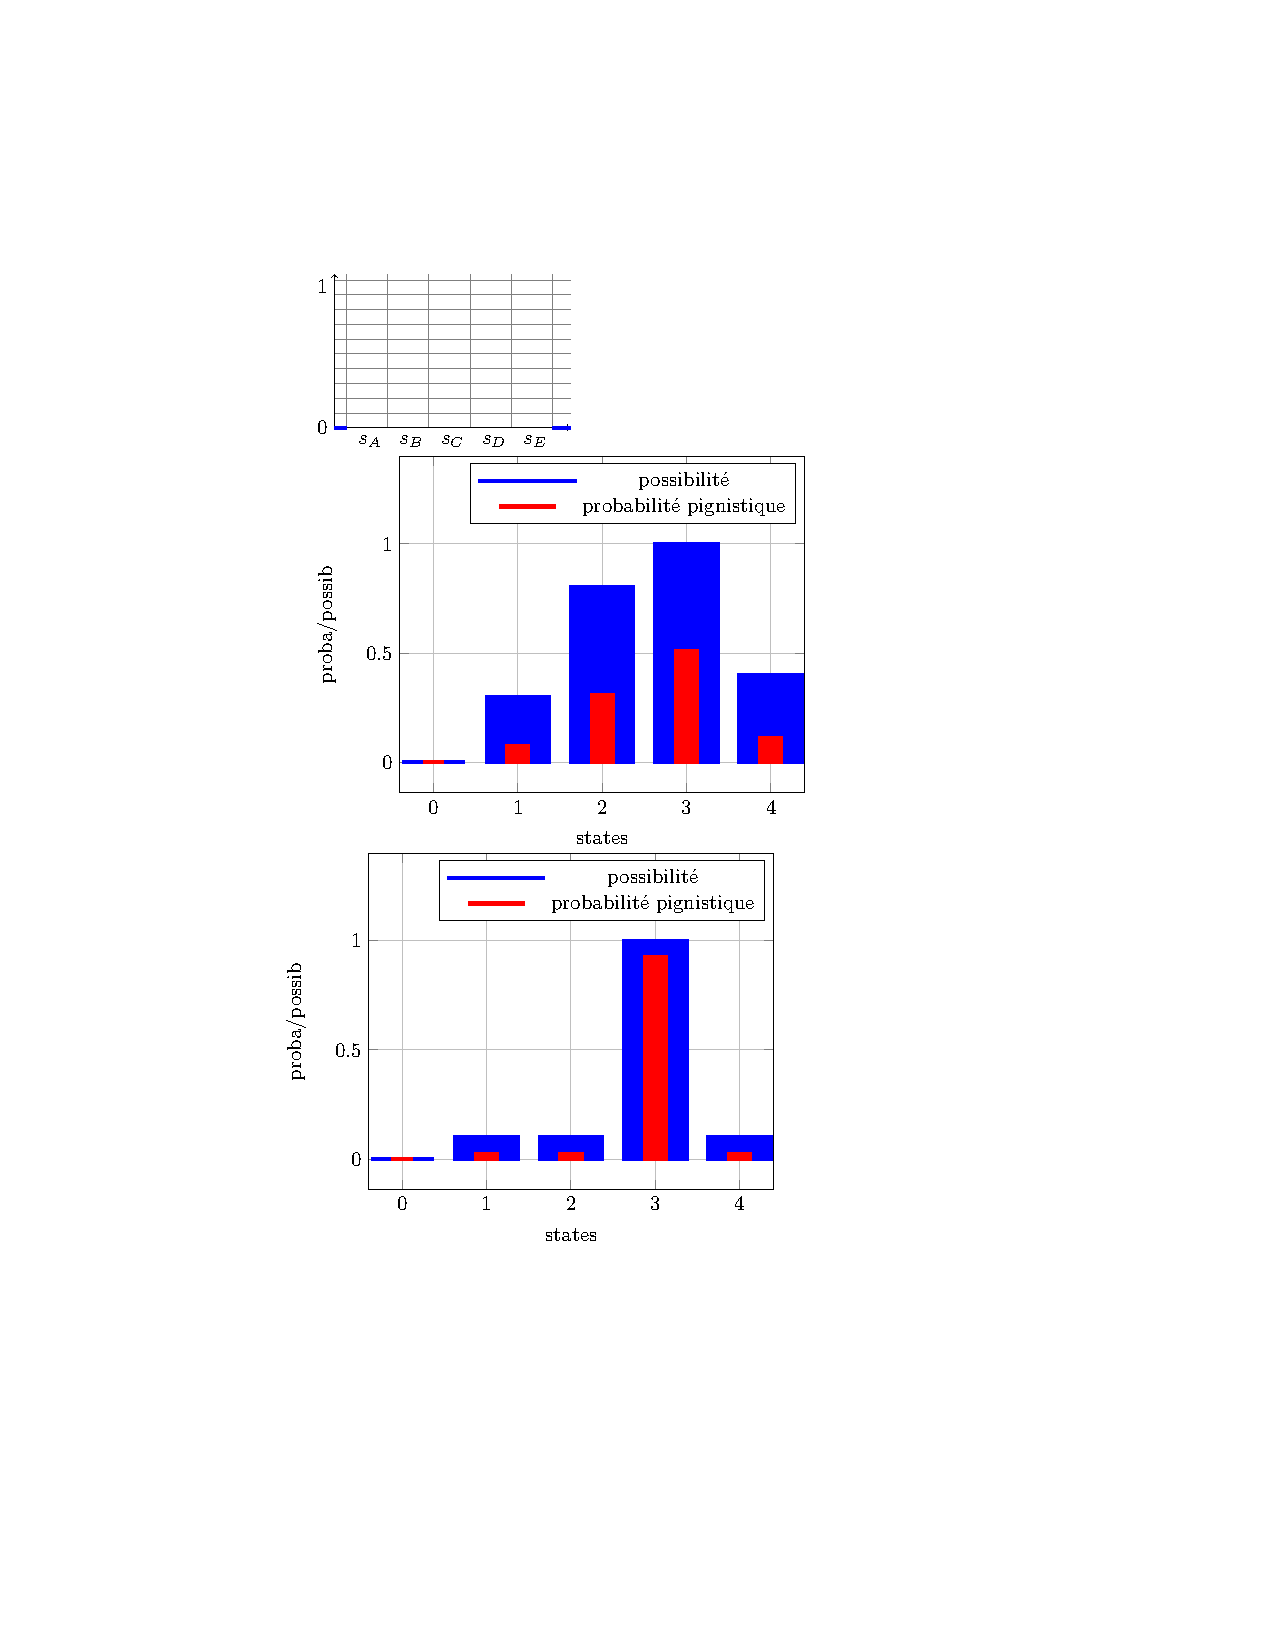
\includegraphics[scale=1.4]{figure.pdf}
\begin{tikzpicture}[transform shape,scale=0.92]
%% vertex shape and color
\tikzstyle{mvertex}=[circle,fill=black!20,minimum size=85pt,inner sep=0pt,draw=black,thick]
\tikzstyle{vertex}=[circle,fill=black!50,minimum size=35pt,inner sep=0pt,draw=black,thick]
\tikzstyle{vvertex}=[circle,fill=black!30,minimum size=35pt,inner sep=0pt,draw=black,thick]
\tikzstyle{avertex}=[rectangle,fill=red!60,minimum size=25pt,inner sep=0pt,draw=black,thick]
\tikzstyle{rvertex}=[fill=yellow!60,decision=3,inner sep=-1pt,minimum size=35pt,draw=black,thick]
\definecolor{darkgreen}{rgb}{0.3,0.8,0.5}
\tikzstyle{overtex}=[circle,fill=blue!50,minimum size=35pt,inner sep=0pt,draw=black,thick]

%% nodes
% states
\node (G-S_1) at (1.3,0) {};
\foreach \name/\x in {S_t/6, S_{t+1}/13}
\node[mvertex] (G-\name) at (\x,0) {};
\node (G-end) at (18.5,0) {};

\foreach \name/\x in {S_{v,t}/5.3, S_{v,t+1}/12.3}
\node[vvertex] (G-\name) at (\x,0) {$\name$};
\node (vG-end) at (16.5,0) {};

\foreach \name/\x in {S_{h,t}/6.7, S_{h,t+1}/13.7}
\node[vertex] (G-\name) at (\x,0) {$\name$};
\node (hG-end) at (16.5,0) {};


\node (ST) at (6,-1) {\begin{huge}$S_{t}$\end{huge}};
\node (STP1) at (13,-1) {\begin{huge}$S_{t+1}$\end{huge}};

% actions
\foreach \name/\x in {a_{t-1}/2,a_t/9}
\node[avertex] (G-\name) at (\x+2.3,-3.5) {$\name$};

% observations
\foreach \name/\x in {O_{h,t}/6,O_{h,t+1}/14.5}
\node[overtex] (G-\name) at (\x+3,3.5) {$\name$};
% visible ones
\foreach \name/\x in {O_{v,t}/2.3,O_{v,t+1}/9.3}
\node[vvertex] (G-\name) at (\x+3,3.5) {$\name$};

%% arrows
% states
\foreach \from/\to in {S_t/S_{t+1}}
\draw[->,>=latex,thick] (G-\from) -- (G-\to);
\foreach \from/\to in {S_1/S_t,S_{t+1}/end}
\draw[->,>=latex,dashed,thick] (G-\from) -- (G-\to);

% actions
\foreach \from/\to in {a_{t-1}/S_t,a_t/S_{t+1}}
\draw[->,>=latex,thick] (G-\from) -- (G-\to);
\foreach \from/\to in {a_{t-1}/O_{h,t},a_t/O_{h,t+1}}
\draw[->,>=latex,thick] (G-\from) to[bend right]  (G-\to);

% observations
\foreach \from/\to in {S_{h,t}/O_{h,t},S_{h,t+1}/O_{h,t+1}}
\draw[->,>=latex,thick] (G-\from) -- (G-\to);
% from visible states
\foreach \from/\to in {S_{v,t}/O_{h,t},S_{v,t+1}/O_{h,t+1}}
\draw[->,>=latex,thick] (G-\from) -- (G-\to);
% from visible states to visible observations
\foreach \from/\to in {S_{v,t}/O_{v,t},S_{v,t+1}/O_{v,t+1}}
\draw[->,>=latex,thick] (G-\from) -- (G-\to);


\node (pis1) at (2.9,0.4) {$\pi \paren{ s_t \sachant s_{t-1}, a_{t-1}  }$};
\node (pis2) at (10,0.4) {$\pi \paren{ s_{t+1} \sachant s_{t}, a_{t}  }$};
\node (pio1) at (7.2,2.5) [rotate=35] {$\pi \paren{ o_{h,t} \sachant s_t,a_{t-1} }$};
\node (pio2) at (15,2.3) [rotate=30] {$\pi \paren{ o_{h,t+1} \sachant s_{t+1},a_{t} }$};

\node (OVEQUALSV) at (4.3,2) {$O_{v,t} = S_{v,t}$};
\node (OVpEQUALSVP) at (11,2) {$O_{v,t+1} = S_{v,t+1}$};
\end{tikzpicture}
\caption[R�seau bay�sien dynamique d'un $\pi$-PDMOM]{
R�seau bay�sien dynamique d'un $\pi$-PDMOM:
� l'�tape de temps $t$,
l'�tat du syst�me est d�crit par la variable $S_t = (S_{v,t},S_{h,t})$.
L'observation re�ue est $O_t=(O_{v,t},O_{h,t})$
avec $O_{v,t}=S_{v,t}$, 
et $O_{h,t}$ d�pend de $S_t$ et de l'action $a_t$.}
\label{piMOMDP}
\end{figure}
La r�solution d'un $\pi$-PDMPO se confronte au fait que
la taille de l'espace des �tats de croyance $\Pi^{\mathcal{S}}_{\mathcal{L}}$ 
est exponentielle en fonction de la taille de l'espace des �tats du syst�me 
$\mathcal{S}$, \textit{cf.} �quation (\ref{equation_numberOfPossDistrib})
de la section \ref{section_piPOMDP}.
Cependant, en pratique,
les �tats du syst�me sont rarement totalement cach�s.
Utiliser la propri�t� d'observabilit� mixte peut �tre une solution:
inspir� par un travail r�cent dans le cadre des PDMPO probabilistes,
\cite{OngShaoHsuWee-IJRR10,AraThoBufCha-ICTAI10}, 
nous pr�sentons dans cette section
un mod�le structur� qui prend en compte
les situations dans lesquelles l'agent observe 
directement une partie de l'�tat du syst�me. 
Un $\pi$-PDMPO qui mod�lise une telle situation respecte la \textit{propri�t� d'observabilit� mixte}.
Les �tats de croyance ne sont alors utilis�s que
pour les composantes partiellement observables
et la taille de l'espace d'�tat est significativement r�suite.
Ainsi, ce mod�le g�n�ralise les $\pi$-PDM et les $\pi$-PDMPO. 

Comme dans \cite{AraThoBufCha-ICTAI10}, 
nous faisons l'hypoth�se que l'espace d'�tat $\mathcal{S}$
d'un PDMOM possibiliste qualitatif ($\pi$-PDMOM)
peut �tre �crit comme le produit cart�sien
d'un espace d'�tats visibles $\mathcal{S}_{v}$ et d'un espace d'�tats cach�s
$\mathcal{S}_h$: $\mathcal{S}$ = 
$\mathcal{S}_v$ $\times$ $\mathcal{S}_h$.
Soit $s=(s_v,s_h)$ un �tat du syst�me. 
La composante $s_v$ est directement observ�e
par l'agent et
$s_h$ est seulement observ� partiellement
� travers les observations de l'ensemble $\mathcal{O}_h$: 
nous notons $\pi_t \paren{o_h' \sachant s',a }$,
la distribution de possibilit� sur l'observation suivante $o_h' \in \mathcal{O}_h$
� l'�tape de temps $t$,
connaissant l'�tat suivant $s' \in \mathcal{S}$ 
et l'action courante $a \in \mathcal{A}$. 
La figure \ref{piMOMDP} illustre la structure 
de ce mod�le � observabilit� mixte. 

L'espace d'�tat visible est identifi� � l'espace des observations: 
$\mathcal{O}_v=\mathcal{S}_v$ 
et $\mathcal{O}$ = $ \mathcal{O}_v \times \mathcal{O}_h$. 
Ainsi, sachant que la composante visible de l'�tat est $s_v$, 
l'agent observe \textit{n�cessairement} $o_v=s_v$ 
($\forall a \in \mathcal{A}$, si $o_v' \neq s_v$, $\pi_t \paren{ o_v' \sachant s_v',a } = 0$).
Formellement, vu comme un $\pi$-PDMPO, 
sa distribution de possibilit� sur les observations 
peut s'�crire:
\begin{eqnarray} 
\nonumber \pi_t \paren{o' \sachant s',a } \hspace{-0.1cm}  & = & \pi_t \paren{ o_v',o_h' \sachant s_v',s_h',a } \\
\nonumber & = & \min \set{ \pi_t \paren{o_h' \sachant s_v',s_h',a }, \pi_t \paren{ o_v' \sachant s_v'} } \\
\label{simplif1}   & = & \left \{ \begin{array}{ccc} 
\pi_t \paren{ o_h' \sachant s',a } & \mbox{if  } o_v' = s_v' \\
0 & \mbox{sinon} 
\end{array} \right. ,
\end{eqnarray}
puisque $\forall a \in \mathcal{A}$, 
$\pi_t \paren{ o_v' \sachant s_v'} = 1$ si $s_v'=o_v'$ et $0$ sinon. 
Le th�oreme suivant, bas� sur cette �galit�,
permet de d�finir les �tats de croyance sur les �tats cach�s du syst�me.
\begin{theorem}[Nature des �tats de croyance atteignables]
\label{thm_natureReachBel} Chaque �tat de croyance atteignable d'un $\pi$-PDMOM
peut �tre �crit comme un �l�ment de 
$\mathcal{S}_v \times \Pi^{\mathcal{S}_h}_{\mathcal{L}}$ 
o� $\Pi^{\mathcal{S}_h}_{\mathcal{L}}$
est l'espace des distributions de possibilit� sur $\mathcal{S}_h$: 
tout $\beta \in \Pi^{\mathcal{S}}_{\mathcal{L}}$ atteignable
peut s'�crire $(s_v,\beta_h)$ 
avec $\beta_h(s_h) = \max_{\overline{s}_v \in \mathcal{S}_v} \beta(\overline{s}_v,s_h)$ 
et $s_v = \operatorname*{argmax}_{\overline{s}_v \in \mathcal{S}_v} \beta(\overline{s}_v,s_h)$.
\end{theorem}

Comme tous les �tats de croyance sont dans $\mathcal{S}_v \times \Pi^{\mathcal{S}_h}_{\mathcal{L}}$
lorsque le $\pi$-PDMPO satisfait la propri�t� d'observabilit� mixte,
le th�or�me suivant r��crit la mise � jour du nouvel �tat de croyance
$\beta_h \in \Pi^{\mathcal{S}}_{\mathcal{L}}$ \textit{i.e.}
de l'�tat de croyance sur les �tats cach�s du syst�me 
$s_h \in \mathcal{S}_h$.
\begin{theorem}[Mise � jour de la croyance pour un $\pi$-PDMOM]
\label{thmMomdpBelup}
Si un probl�me peut se mod�liser par un $\pi$-PDMOM  
\[ \Big\langle S_v \times S_h, \mathcal{A}, \mathcal{O}_h, T^{\pi}, O^{\pi}, \Psi, \beta_0 = (s_{v,0}, \beta_{h,0})  \Big\rangle, \]
une nouvelle fonction de mise � jour de l'�tat de croyance $\nu_h$
peut �tre d�finie:
si, � l'�tape de temps $t$,
l'�tat visible courant est $s_{v,t} \in \mathcal{S}_v$,
l'�tat de croyance courant sur l'�tat cach� est 
$\beta_{h,t} \in \Pi^{\mathcal{S}_h}_{\mathcal{L}}$,
l'action choisie courante est $a_t \in \mathcal{A}$,
l'�tat visible suivant est $s_{v,t+1} \in \mathcal{S}_v$
et l'observation suivante est $o_{h,t+1} \in \mathcal{O}_h$,
alors l'�tat de croyance suivant
� propos de l'�tat cach� du syst�me est
\begin{equation}
\label{equation_piMOMDPupdate}
\beta_{h,t+1}(s_h') = \left \{ \begin{array}{ccc}
1 & \mbox{ si } \left. \begin{array}{cc} \pi_t \paren{ s_h', s_{v,t+1}, o_{h,t+1} \sachant s_{v,t}, \beta_{h,t}, a_t } \\
	 	= \pi_t \paren{s_{v,t+1}, o_{h,t+1} \sachant s_{v,t}, \beta_{h,t}, a_t }
		\end{array} \right., \\
\\
\pi_t \paren{ s_h', s_{v,t+1}, o_{h,t+1} \sachant s_{v,t}, \beta_{h,t}, a_t } & \mbox{ sinon } 
\end{array} \right. 
\end{equation}
o�
\[ \pi_t \paren{s_v',  s_h', o_h' \sachant s_v, \beta_h, a } = \min \Big\{ \pi_t \paren{ o_h' \sachant s', a  }, \max_{s_h \in \mathcal{S}_h} \min \set{ \pi_t \paren{s' \sachant s_v,s_h, a}, \beta_h(s_h)  } \Big\} \] 
est la distribution de possibilit� jointe sur les �tats du syst�me $s_h' \in \mathcal{S}_h$
et les objets visibles (�tat visible du syst�me et observation) $s_v' \in \mathcal{S}_v$ et $o_h' \in \mathcal{O}_h$.
La mise � jour de l'�tat de croyance est not�e \[ \beta_h' = \nu_h \paren{ s_v, \beta_h, a, s_v', o_h' }. \]
\end{theorem}

L'espace d'�tat du $\pi$-PDM r�sultant d'un $\pi$-PDMOM
peut alors �tre restreint � l'espace produit 
$\mathcal{S}_v \times \Pi^{\mathcal{S}_h}_{\mathcal{L}}$,
\textit{i.e.} 
un espace d'�tat plus petit gr�ce
� l'observabilit� mixte: 
le $\pi$-PDM r�sultant est
$\langle \tilde{S}^{\pi}, \tilde{T^{\pi}}, \mathcal{A}, \tilde{\Psi} \rangle$,
o�
\begin{itemize}
\item l'espace des �tats du syst�me est $\tilde{S}^{\pi} = \mathcal{S}_v \times \Pi^{\mathcal{S}_h}_{\mathcal{L}}$,
\item la distribution de probabilit� de transition dans $\tilde{T^{\pi}}$ 
est telle que $\forall \set{ 0, \ldots, H-1 }$, $\forall a \in \mathcal{A}$,
$\forall \Big[ (s_v,\beta_h), (s_v',\beta_h') \Big]  \in \Big(\tilde{S}^{\pi}\Big)^2$, 
\[ \pi_t \Big( (s_v',\beta_h') \Big\vert (s_v,\beta_h), a  \Big) = \max_{\substack{ o_h' \in \mathcal{O}_h \mbox{ \tiny s.t. } \\ \nu_h(s_v,\beta_h,a,s_v',o_h') = \beta_h'}}
\pi_t \paren{ s_v',o_h' \sachant s_v, \beta_h, a },  \]
o� $\pi_t \paren{ s_v',o_h' \sachant s_v, \beta_h, a }$ est d�fini dans le th�or�me au-dessus,
\item la pr�f�rence pessimiste \textit{i.e.}
$\tilde{\Psi}=\underline{\Psi}$: elle peut �tre r��crite $\forall s_v \in \mathcal{S}_v$,
$\forall \beta_h \in \Pi^{\mathcal{S}_h}_{\mathcal{L}}$, $\forall a \in \mathcal{A}$,  
\[ \underline{\Psi}(s_v,\beta_h) = \min_{s_h \in \mathcal{S}_h} \max \set{ \Psi(s_v,s_h), 1 - \beta_h(s_h) }. \]
\end{itemize}

Un algorithme standard aurait calcul� la fonction valeur pour chaque
 $\beta \in \Pi^{\mathcal{S}}_{\mathcal{L}}$ 
tandis que l'�quation de programmation dynamique
du $\pi$-PDM r�sultant
m�ne � un algorithme
qui la calcule
seulement pour chaque $(s_v,\beta_h) \in \mathcal{S}_v \times 
\Pi^{\mathcal{S}_h}_{\mathcal{L}}$,
puisque seuls ces �tats de croyance sont atteignables.
La taille du nouvel espace des �tats de croyance est
\[ \# (\mathcal{S}_v \times \Pi^{\mathcal{S}_h}_{\mathcal{L}})
= \# \mathcal{S}_v \times \paren{ \# \mathcal{L}^{\# \mathcal{S}_h} - (\# \mathcal{L}-1)^{\# \mathcal{S}_h} }, \] 
ce qui est exponentiellement plus petit que
la taille de l'espace des �tats de croyance 
du $\pi$-PDMPO �quivalent: 
\[ \# \Pi^{\mathcal{S}}_{\mathcal{L}} = \# \mathcal{L}^{\# \mathcal{S}_v \times \# \mathcal{S}_h} - (\# \mathcal{L}-1)^{\# \mathcal{S}_v \times \# \mathcal{S}_h}. \]

\section{Horizon Ind�termin�}
\label{section_infiniteHorizon}
Pour de nombreux probl�mes en pratique,
il est tr�s difficile de d�terminer un horizon $H$.
Le but de cette section est de pr�senter
un algorithme pour r�soudre les $\pi$-PDMOM 
avec pr�f�rence terminale,
et horizon ind�termin�.

\begin{algorithm} \caption{Algorithme IV pour $\pi$-PDM -- Pr�f�rence Terminale} 
\label{algorithmIVPIMDP}
\For {$s \in \mathcal{S}$}{
	$\overline{U^*}(s) \gets 0$ \;
	$\overline{U^c}(s) \gets \Psi(s)$ \;
	$\overline{\delta^*}(s) \gets \widehat{a}$ \;
}
\While {$\overline{U^*} \neq \overline{U^c}$ }{
\label{beginning_while_VI}	$\overline{U^*}=\overline{U^c}$ \;
	\For {$s \in \mathcal{S}$}{
		$\displaystyle \overline{U^c}(s) \gets \max_{a \in \mathcal{A}} \max_{s' \in \mathcal{S}} \min \set{ \pi \paren{ s' \sachant s,a }, \overline{U^*}(s') }$ \label{VIupdate_OptAlgo} \;
		\If {$\overline{U^c}(s)>\overline{U^*}(s)$}{
			$ \displaystyle \overline{\delta^*}(s) \in \operatorname*{argmax}_{a \in \mathcal{A}} \max_{s' \in \mathcal{S}} \min \set{ \pi \paren{ s' \sachant s,a }, \overline{U^*}(s') }$ \;
 		}
 	}
}
\Return $\overline{U^*}$, $\overline{\delta^*}$ \;
\end{algorithm}

\`A notre connaissance,
nous proposons ici le premier algorithme d'it�ration sur les valeurs (IV)
pour $\pi$-PDM
qui renvoie une strat�gie optimale pour un crit�re sp�cifi�.
Comme mentionn� dans \cite{Sabbadin1999pipomdp}, 
nous faisons l'hypoth�se de l'existence d'une action
``rester'', not�e $\widehat{a}$, 
qui retient le syst�me dans son �tat courant 
avec n�cessit� $1$. 
Cette action est l'homologue possibiliste
du facteur d'actualisation $\gamma$ 
dans le mod�le probabiliste,
puisqu'il garantit la convergence
de l'algorithme d'it�ration sur les valeurs. 
Nous verrons cependant que l'action $\widehat{a}$
n'est finalement utilis�e que sur certains �tats buts.
Notons qu'une hypoth�se similaire est utilis�e
pour calculer des strat�gies optimales
dans le cadre des processus d�terministes (planification classique) 
dont l'horizon
n'est pas sp�cifi� \cite{LaValle2006PA1213331}.

Nous notons $\widehat{\delta}$
la r�gle de d�cision telle que
$\forall s \in \mathcal{S}$, $\widehat{\delta}(s)=\widehat{a}$. 
L'ensemble fini de toutes les stat�gies
est
$\Delta =\cup_{i \geqslant 1} \Delta_i$, 
et $\# \delta$ est la taille de la strat�gie $(\delta)$ 
en termes d'�tapes de d�cision. 
Nous pouvons maintenant d�finir le crit�re optimiste
pour un horizon ind�termin�: 
si $(\delta) \in \Delta$,
\begin{equation} 
\label{optcriterion} 
\overline{U} \Big( s_0,(\delta) \Big) 
= \max_{ \mathcal{T} \in \mathcal{T}_{\# \delta}} 
\min \bigg\{ \pi \Big( \mathcal{T} \Big\vert s_0, (\delta) \Big), \Psi(s_{\# \delta}) \bigg\},
\end{equation}
o� $\mathcal{T} = (s_1,\ldots,s_{\# \delta})$ 
est une trajectoire d'�tats du syst�me,
$\mathcal{T}_{\# \delta}$ 
l'ensemble de telles trajectoires,
et 
\[ \pi \Big( \mathcal{T} \Big\vert s_0, (\delta) \Big) 
= \min_{i=0}^{\# \delta - 1} \pi \Big( s_{i+1} \Big\vert s_i, \delta_i(s_i)  \Big). \]
\begin{theorem}[Optimalit� de l'algorithme d'IV pour les $\pi$-PDM optimistes]
\label{thmIV} Si il existe une action $\widehat{a}$ 
telle que, 
pour chaque $s \in \mathcal{S}$, $\pi \paren{s' \sachant s, \widehat{a} } = 1$ 
si $s'=s$ et $0$ sinon, 
alors l'algorithme \ref{algorithmIVPIMDP} 
calcule le crit�re maximal 
et une strat�gie optimale,
\textit{i.e.} qui maximise le crit�re (\ref{optcriterion}),
et qui est stationnaire 
(\textit{i.e.} qui ne d�pend pas de l'�tape du processus $t$).
\end{theorem}

Soit $s$ un �tat tel que $\overline{\delta^*}(s)=\widehat{a}$, 
o� $\overline{\delta^*}$ est la strat�gie renvoy�e par l'algorithme. 
En regardant l'algorithme \ref{algorithmIVPIMDP}, 
nous pouvons remarquer que $\overline{U^*}(s)$ 
reste �gal � $\Psi(s)$
durant les it�rations de l'algorithme 
apr�s le premier passage dans la boucle while.
Donc, $\forall s' \in \mathcal{S}$, 
soit $\forall a \in \mathcal{A}$, 
$\Psi(s) \geqslant \pi \paren{s' \sachant s,a}$, 
soit $\Psi(s) \geqslant \overline{U^*}(s')$. 
Si le probl�me n'est pas trivial,
cela signifie que $s$ est un but ($\Psi(s)>0$)
et que les degr�s de possibilit� de transition vers de meilleurs buts
sont plus petit que le degr� de pr�f�rence de $s$. 

\section{R�sultats \'Exp�rimentaux}
Consid�rons un robot sur une grille de taille $g \times g$, avec $g>1$. 
Il connait parfaitement sa position sur la grille $(x,y) \in \{ 1, \ldots, g \}^2$ � chaque �tape du processus, 
ce qui constitue l'espace des �tats visibles $\mathcal{S}_v$. 
Il se trouve initialement � la position $s_{v,0}=(1,1)$. 
Deux cibles immobiles sont pr�sentes sur la grille:
la ``cible $1$'' est en $(x_1,y_1)=(1,g)$, 
la ``cible $2$'' se trouve en $(x_2,y_2)=(g,1)$ sur la grille,
et le robot connait parfaitement leurs positions. 
Une des deux cibles est $A$, l'autre est $B$, 
et la mission du robot est d'identifier et d'atteindre $A$ 
aussi t�t que possible. 
Le robot ne sait pas quelle cible est $A$: 
les deux situations $A_1$ et $A_2$
correspondent respectivement � ``la cible $1$ est $A$'' 
et ``la cible $2$ est $A$'' et
constituent l'espace des �tats cach�s $\mathcal{S}_h$. 
Les actions $\mathcal{A}$ sont les d�placements 
dans les quatre directions ainsi que l'action ``rester'';
les d�placements du robot sont d�terministes.
A chaque �tape du processus, le robot analyse une image de chaque cible
et obtient alors une observation de la nature de la cible:
les deux cibles peuvent sembler �tre $A$ ($oAA$), 
ou bien seulement la cible $1$ ($oAB$), 
ou seulement la cible $2$ ($oBA$),
ou alors aucune des deux ($oBB$).

Dans le cadre probabiliste, 
la probabilit� de recevoir une bonne observation de la cible $i \in \{ 1,2 \}$, 
n'est pas vraiment connue, mais est approch�e par
$Pr \paren{ good_i \sachant x,y } = \frac{1}{2} \croch{ 1 + \exp \paren{ -\frac{\sqrt{(x-x_i)^2+(y-y_i)^2}}{D} } } $ 
o� $(x,y)$ $=s_v$ $\in \{ 1,\ldots,g \}^2 $ est la position du robot, 
$(x_i,y_i)$ la position de la cible $i$, 
et $D>0$ une constante de normalisation.
Les processus d'observation de chaque cible sont consid�r�s ind�pendants. 
Alors, par exemple, $Pr \paren{ oAB \sachant \hspace{-0.1cm} (x,y), A_1 }$ 
est �gal � $Pr \paren{ good_1 \sachant \hspace{-0.1cm} (x,y)} 
\cdot Pr \paren{ good_2 \sachant \hspace{-0.1cm} (x,y) }$, 
$Pr \paren{ oAA \sachant \hspace{-0.1cm} (x,y), A_1 }$ � 
$Pr \paren{ good_1 \sachant \hspace{-0.1cm} (x,y)} 
\cdot \croch{ 1 - Pr \paren{ good_2 \sachant \hspace{-0.1cm} (x,y) } } $, etc. 
Chaque �tape du processus avant d'atteindre une cible co�te $1$, 
atteindre la cible $A$ et y rester est r�compens� par $100$, 
et par $-100$ pour $B$. 
La strat�gie provenant du mod�le probabiliste
a �t� calcul�e en tenant compte de l'Observabilit� Mixte du probl�me,
avec APPL \cite{OngShaoHsuWee-IJRR10}, 
en utilisant une pr�cision de $0.046$ 
(la limite en m�moire est atteinte pour une pr�cision sup�rieure) 
et $\gamma=0.99$. 
Ce probl�me ne peut pas �tre r�solu par l'algorithme exact pour PDMOM \cite{AraThoBufCha-ICTAI10}
puisque cela entra�ne l'utilisation de toute la m�moire vive disponible apr�s 15 it�rations.

Avec la th�orie des possibilit�s qualitatives,
il est toujours possible d'observer correctement la cible: 
$\pi \paren{good \sachant x,y}=1$. 
Ensuite, plus le robot est loin de la cible $i$,
plus il est susceptible de mal l'observer 
(par exemple observer $A$ au lieu de $B$), 
ce qui est une hypoth�se raisonnable 
compte tenu du fait que le mod�le d'observation
est mal connu: $\pi \paren{ bad_i \sachant \hspace{-0.1cm} x,y } = \frac{\sqrt{(x-x_i)^2 + (y-y_i)^2 }}{\sqrt{2}(g-1)}$. 
Ainsi, par exemple, 
$\pi \paren{ oAB \sachant \hspace{-0.1cm} (x,y), A_1 \hspace{-0.07cm} }=1$, 
$\pi \paren{ oAA \sachant \hspace{-0.1cm} (x,y), A_1 \hspace{-0.07cm} } 
= \pi \paren{ bad_2 \sachant \hspace{-0.1cm} x,y } $, 
$\pi  \paren{ oBA \sachant (x,y), A_1 } 
= \min \{ \pi \paren{ bad_1 \sachant x,y },$ 
$\pi \paren{ bad_2 \sachant x,y } \} $, etc.
Puisque la situation est compl�tement connue lorsque le robot est sur la position d'une cible (observation d�terministe), 
il n'y a pas de risque d'�tre bloqu� dans un �tat non satisfaisant,
et c'est pourquoi le mod�le $\pi$-PDMOM \textit{optimiste} fonctionne bien.
L'�chelle $\mathcal{L}$ est compos�e de $0$, $1$, 
et toutes les valeurs possibles de $\pi \paren{ bad_i \sachant x,y } \in [0,1]$. 
Notons qu'une construction de ce mod�le
avec une transformation probabilit�-possibilit� \cite{Dubois93onpossibilityprobability} 
aurait �t� �quivalente. 
La distribution de pr�f�rence $\Psi$ est �gale � $0$ pour tous les �tats du syst�me,
et � $1$ pour les �tats $[(x_{1},y_{1}),A_1]$ et $[(x_{2},y_{2}),A_2]$ o� $(x_{i},y_{i})$ 
est la position de la cible $i$. 
Comme mentionn� dans \cite{Sabbadin1999pipomdp}, 
la strat�gie calcul�e garantit un plus court chemin vers les �tats buts:
la strat�gie tend � r�duire le temps de la mission.
%First, consider a $3 \times 3$-grid. There are $9$ visible states 
%and $2$ hidden one: $\# \mathcal{S} = 18$. $\mathcal{L} = 5$ so $\# B^{\pi} = 18^5$ 

Les algorithmes pour $\pi$-PDMPO standards, qui n'exploitent pas l'observabilit� mixte
contrairement � notre mod�le $\pi$-PDMOM, ne peuvent pas r�soudre le probl�me
m�me pour de tr�s petites grilles $3 \times 3$. 
En effet, pour ce probl�me, $\# \mathcal{L} = 5$, $\# \mathcal{S}_v = 9 $, 
et $\# \mathcal{S}_h = 2$. 
Ainsi, $\# \mathcal{S} = \# \mathcal{S}_v \cdot \# \mathcal{S}_h = 18$ 
et le nombre d'�tats de croyance est alors 
$\# \Pi^{\mathcal{S}}_{\mathcal{L}} = \mathcal{L}^{\# \mathcal{S}} - (\mathcal{L}-1)^{\# \mathcal{S}} = 5^{18} -4^{18} \geqslant 3.7.10^{12} $ 
au lieu de $81$ �tats
avec un $\pi$-PDMOM. 
Par cons�quent, les r�sultats exp�rimentaux qui suivent n'auraient pas pu �tre obtenus
avec des $\pi$-PDMPO standards, ce qui justifie donc ce travail sur les $\pi$-PDMOM.

La comparaison des performances des mod�les probabilistes et possibilistes
peut se faire � l'aide des esp�rances de la somme des r�compenses 
de leurs strat�gies respectives:
puisque la situation est compl�tement connue lorsque le robot est � la position d'une des cibles, 
il ne peut pas terminer en choisissant la cible $B$. 
Si $k$ est le nombre d'�tapes du processus pour identifier et atteindre la bonne cible, 
alors la somme des r�compenses est $100-k$. 

Consid�rons maintenant qu'en r�alit� (donc ici pour les simulations),
et contrairement � ce qui est d�crit par le mod�le, 
la situation en pratique fait que l'algorithme de vision artificielle utilis� par le robot 
est trompeur lorsque le robot est loin des cibles, 
\textit{i.e.} si $\forall i \in \{1,2\}$, $\sqrt{(x-x_i)^2+(y-y_i)^2}>C$, 
avec $C$ une constante positive, alors
$Pr \paren{good_i \sachant x,y }$ 
$= 1-P_{bad} < \frac{1}{2}$.  
Dans tous les autres cas, 
le mod�le probabiliste est bien d�crit, \textit{i.e.} en accord avec la r�alit�.
La figure \ref{exprobot} r�sume le probl�me,
et indique la zone o� le robot a une mauvaise perception
par la d�nomination ``error zone''.
Pour les exp�rimentations num�riques qui suivent,
le nombre de simulations �tait de $10^4$ 
pour calculer la moyenne de la somme des r�compenses � l'ex�cution. 
La taille de la grille �tait de $10 \times 10$, $D=10$ et $C=4$. 

\begin{figure}
\centering
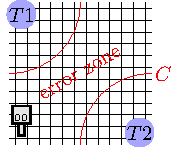
\includegraphics[width=0.35\linewidth]{robotgrid.pdf} 
\caption[Mission robotique de reconnaissance de cibles]{Mission robotique de reconnaissance de cibles:
deux cibles, la cible $1$ (T1) et la cible $2$ (T2) 
sont dispos�es sur une grille $g \times g$. 
Une des deux cibles est l'objet d'int�r�t $A$,
(et par �limination, l'autre cible est $B$):
soit $T1=A$, soit $T2=A$. 
Le robot re�oit des observations sur la nature de chaque cible: 
``$Ti=A$'' ou $``Ti=B''$ pour $i \in \set{1,2}$, de mani�re bruit�e.
Plus le robot est proche d'une cible, moins l'observation � propos de la cible en question a de chances d'�tre fausse.
Le robot doit reconna�tre la cible $A$ et l'atteindre. 
Cependant, sans avoir pu �tre pris en compte dans le mod�le, 
lorsque le robot est dans une zone d'erreur (\textit{error zone} en rouge)
la probabilit� qu'il observe mal $P_{bad}$ est sup�rieure � $0.5$}
\label{exprobot}
\end{figure}

La figure \ref{figureexp}.a montre que le mod�le probabiliste est plus affect� par l'erreur introduite
que le mod�le possibiliste: 
elle repr�sente la moyenne de la somme des r�compenses � l'ex�cution 
obtenue par chaque mod�le, comme une fonction de $P_{bad}$, 
la probabilit� de mal observer une cible lorsque la position 
du robot est telle que $\sqrt{(x-x_i)^2+(y-x_i)^2} >C$. 
Cela est d� au fait que la mise � jour possibiliste de l'�tat de croyance 
ne tient pas compte des nouvelles observations
lorsque le robot en a d�j� obtenu une plus fiable. 
Au contraire, le mod�le probabiliste modifie l'�tat de croyance courant � chaque �tape.
En effet, puisqu'il n'y a que deux �tats cach�s $s_h^1$ et $s^2_h$, 
si $\beta_{h}(s_{h}^1)<1$, alors la normalisation possibiliste implique que $\beta_{h}(s_{h}^2)=1$. 
La d�finition de la possibilit� jointe de l'�tat et de l'observation 
(le minimum entre la distribution de possibilit� sur l'�tat du syst�me, \textit{i.e.} l'�tat de croyance, 
et la possibilit� de l'observation) 
assure que la possibilit� jointe 
de $s_{h}^1$ et de l'observation obtenue, 
est plus petite que $\beta_{h}(s_{h}^1)$. 
L'�quivalent possibiliste de l'�quation de mise � jour de l'�tat de croyance (3) 
assure donc que l'�tat de croyance suivant 
se retrouve dans un des trois cas suivant: 
\begin{itemize}
\item il est encore plus sceptique � propos de $s_{h}^1$ 
si l'observation est plus fiable, et confirme l'�tat de croyance pr�c�dent 
($\pi \paren{o_h \sachant s_v,s_h^1,a }$ est plus petit que $\beta_{h}(s_{h}^1)$); 
\item il devient l'�tat de croyance oppos� si l'observation est plus fiable et contredit l'�tat de croyance pr�c�dent 
($\pi \paren{o_h \sachant s_v,s_h^2,a }$ est � la fois plus petit que $\beta_{h}(s_{h}^1)$ et que $\pi \paren{o_h \sachant s_v,s_h^1,a }$); 
\item il reste simplement le m�me
si l'observation n'est pas plus informative
que l'�tat de croyance courant.
\end{itemize} 
Le th�or�me qui suit donne des conditions suffisantes 
menant � une mise � jour
informative de l'�tat de croyance possibiliste.
Classiquement un �tat de croyance $\beta_1 \in \Pi^{\mathcal{S}}_{\mathcal{L}}$ 
est dit plus sp�cifique qu'un �tat de croyance $\beta_2 \in \Pi^{\mathcal{S}}_{\mathcal{L}}$
si pour chaque $ s \in \mathcal{S}$, $\beta_1(s) \leqslant \beta_2(s)$.
La relation d'ordre $\preceq$ sur $\Pi^{\mathcal{S}}_{\mathcal{L}}$ peut alors �tre d�finie 
pour classer les �tats de croyance selon leur sp�cificit�:
\[\beta_1 \preceq \beta_2 \Leftrightarrow \sum_{s \in \mathcal{S}} \beta_1(s) \leqslant \sum_{s \in \mathcal{S}} \beta_2(s)  \]
Notons que si $\beta_1$ est plus sp�cifique que $\beta_2$, alors $\beta_1 \preceq \beta_2$.
\begin{theorem}
Soit $\beta_0 \in \Pi^{\mathcal{S}}_{\mathcal{L}}$ l'�tat de croyance initial 
mod�lisant l'ignorance totale, \textit{i.e.} pour tous les $ s \in \mathcal{S}$, $\beta_0(s)=1$.
Si la fonction de transition est d�terministe,
et si les observations ne sont pas informatives, \textit{i.e.} 
 $\forall s' \in \mathcal{S}$ , $\forall a \in \mathcal{A}$, $\forall o' \in \mathcal{O}$, 
$\pi \paren{o' \sachant s',a}=1$,
alors si l'�tat de croyance $\beta_{t+1} \in \Pi^{\mathcal{S}}_{\mathcal{L}}$ 
est le r�sultat de la mise � jour de l'�tat de croyance 
$\beta_t \in \Pi^{\mathcal{S}}_{\mathcal{L}}$, $\beta_{t+1} \preceq \beta_{t}$.
Ce r�sultat reste valable si pour chaque action la fonction de transition est l'identit�
et $\forall (o',\tilde{o}) \in \mathcal{O}^2$, $\forall (a,\overline{a}) \in \mathcal{A}^2$ et
$\forall s' \neq  \tilde{s} \in \mathcal{S}$ 
t.q. $\pi \paren{o' \sachant s',a} < 1_{\mathcal{L}}$,
$\pi \paren{o' \sachant s',a} \neq \pi \paren{ \tilde{o} \sachant \tilde{s}, \overline{a}}$.
\label{theorem_specificity_belief}
\end{theorem}
La mise � jour probabiliste quant � elle
ne permet pas � l'�tat de croyance de devenir directement l'�tat de croyance oppos�,
ou d'ignorer les observations moins fiables: 
le robot se dirige d'abord vers la mauvaise cible
car il est initialement trop loin des deux cibles
et les observe mal. 
Lorsqu'il est proche de cette cible, il re�oit de bonnes observations, 
et change petit � petit d'�tat de croyance: 
ce dernier devient assez informatif 
pour le convaincre de se diriger vers la cible $A$. 
Cependant, il passe alors in�vitablement par la zone d'erreur: 
cela modifie peu � peu son �tat de croyance, 
qui devient faux avec grande probabilit�, 
et le robot se retrouve dans la situation initiale.
Il perd ainsi beaucoup de temps � sortir de cette boucle. 
On peut voir que la moyenne de la somme des r�compenses cro�t lorsque la probabilit�
de mal observer, $P_{bad}$, est tr�s grande: 
cela s'explique par le fait que cette grande erreur
m�ne le robot � atteindre la mauvaise cible plus rapidement, 
et donc � �tre quasiment s�r que la cible $A$ est l'autre cible.
\begin{figure}
\begin{tabular}{cc}
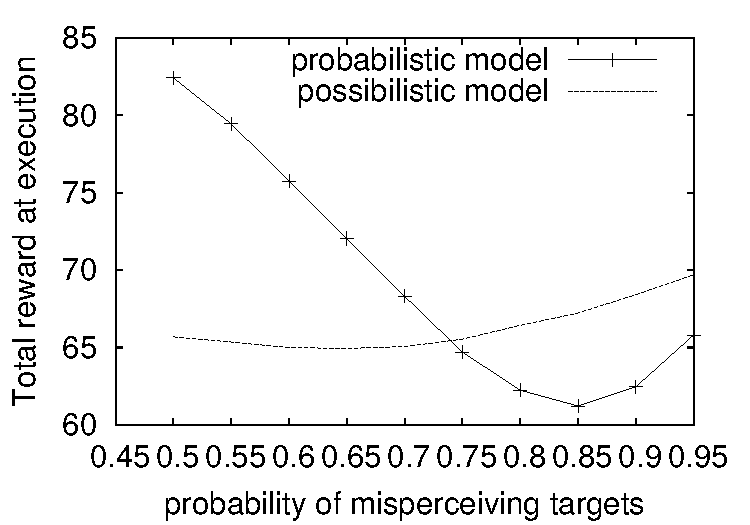
\includegraphics[width=.45\linewidth]{courbe1.pdf} &
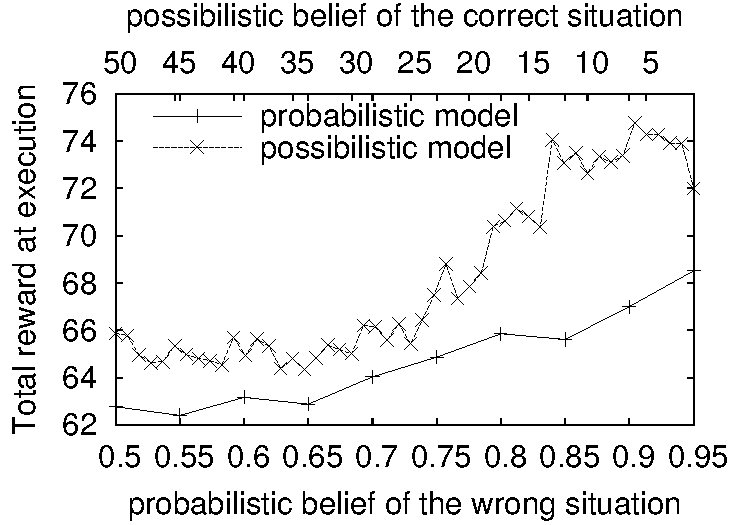
\includegraphics[width=.45\linewidth]{courbe2.pdf} \\
(a) $P_{bad}$ varie  & (b) $\beta_0$ varie, $P_{bad} = 0.8$
\end{tabular}
\caption[Comparaison des moyennes de la somme des r�compenses � l'ex�cution, pour les mod�les probabilistes et possibilistes.]{Comparaison des moyennes de la somme des r�compenses � l'ex�cution, pour les mod�les probabilistes et possibilistes.}
\label{figureexp}
\end{figure}

Maintenant, fixons $P_{bad}=0.8$ 
et �valuons la moyenne de la somme des r�compenses � l'ex�cution
pour diff�rents faux �tats de croyance initiaux: 
la figure \ref{figureexp}.b illustre cette �valuation,
avec les m�mes param�tres que pour la pr�c�dente exp�rimentation: 
nous comparons ici le mod�le possibiliste, et la probabiliste
lorsque l'�tat de croyance initial est fortement orient�e
vers la mauvaise cible (\textit{i.e.} l'agent pense fortement que la cible $1$ est $B$ alors que c'est $A$ en r�alit�). 
Notons que l'�tat de croyance possibiliste en la bonne cible d�cro�t 
lorsque la n�cessit� en la mauvaise cro�t. 
Cette figure montre que le mod�le possibiliste 
m�ne � de meilleures r�compenses � l'ex�cution
si l'�tat de croyance initial est mauvais
et la fonction d'observation est impr�cise:
notons cependant que pour $\mathcal{P}_{bad} \leqslant 0.6$,
la politique probabiliste est plus efficace~\footnote{L'impl�mentation de l'algorithme de r�solution, 
ainsi que la description de ce probl�me de reconnaissance qui en est l'entr�e, 
sont disponibles sur le d�p�t accessible � l'adresse \url{https://github.com/drougui/ppudd}:
le probl�me peut �tre simul� en utilisant la strat�gie optimale possibiliste calcul�e par l'algorithme.}.

\section{Conclusion}
Nous avons propos� un algorithme d'It�ration sur les Valeurs (IV) pour les PDM possibilistes.
Celui-ci calcule une strat�gie optimale stationnaire pour un horizon ind�termin�
contrairement aux m�thodes pr�c�dentes. 
Une preuve compl�te de la convergence a �t� fournie:
elle repose sur l'existence d'une action ``rester''
interm�diaire. Celle-ci est utilis�e uniquement pour maintenir le processus dans les �tats buts.
Enfin, le nouveau mod�le des PDM possibilistes qualitatifs � observabilit� mixte, 
a �t� pr�sent�, et sa complexit� est exponentiellement plus petite que celle des PDMPO
possibilistes qualitatifs.
De ce fait, nous avons pu comparer les $\pi$-PDMOM avec leurs �quivalents probabilistes 
sur un probl�me robotique r�aliste. 
Nos r�sultats exp�rimentaux montrent que ces strat�gies possibilistes
peuvent �tre plus performantes que les strat�gies issues du mod�le probabiliste
lorsque la fonction d'observation n'est pas connue pr�cis�ment. 

La version de l'algorithme d'It�ration sur les Valeurs pour $\pi$-PDM  pessimiste 
peut aussi �tre construite,
mais l'optimalit� de la strat�gie renvoy�e
semble dure � prouver.
Les travaux \cite{LIP61498} et \cite{0024909} 
peuvent �tre utiles pour obtenir des r�sultats
� propos de ces $\pi$-PDM pessimistes,
afin de r�soudre des probl�mes contenant des situations dangereuses.

Finalement, comme cela a �t� mis en �vidence par les exp�riences,
bien que les $\pi$-PDMPO soient
bas�s sur un mod�le d'incertitude plus simple en termes de complexit�
que les PDMPO probabilistes,
le processus de croyance
peut avoir un comportement int�ressant.
Pour certaines conditions suffisantes
donn�es par le th�or�me \ref{theorem_specificity_belief},
l'�tat de croyance n'est pas modifi�
par des informations moins fiables
que celles accumul�es avant elles, 
mais est capable de se transformer en un �tat de croyance quasi oppos� 
si une information qui le sugg�re et qui est plus fiable est re�ue.
Des probl�mes plus complexes doivent �tre �tudi�s
pour avoir une meilleure id�e de son comportement
dans un panel de situations plus important.
Cependant, les $\pi$-PDMPO avec un espace d'�tat trop grand
(ou $\pi$-PDMOM avec un trop grand espace $\mathcal{S}_h$)
ne peuvent pas �tre r�solus en temps raisonnables 
par les algorithmes d�velopp�s jusqu'� aujourd'hui.
Le chapitre suivant pr�sente et utilise
d'autres structures du probl�me,
d�crites par l'homologue possibiliste qualitatif 
du mod�le des \textit{PDMPO factoris�s}:
ces structures m�nent � des calculs de strat�gies possibilistes plus simples,  
et permettent de r�soudre de nombreux probl�mes de planification.


% ============================================================
% 
\chapter{D\'eveloppement d'Algorithmes pour la r\'esolution des $\pi$-POMDPs}
%%%%%%%%%%%%%%%%%%%%%%%%%%%%%%%%%%%%%%%%%%%%%%%%%%%%%%%%%%%%%%%%%%%%%%%
% TODO TODO TODO TODO TODO TODO TODO TODO TODO TODO TODO TODO TODO TODO
%%%%%%%%%%%%%%%%%%%%%%%%%%%%%%%%%%%%%%%%%%%%%%%%%%%%%%%%%%%%%%%%%%%%%%%
\label{chap_symb}
%Dans ce chapitre, nous proposons
l'�tude des mod�les $\pi$-PDMOM 
dans le but de r�soudre 
de tr�s grands probl�mes de planification
lorsqu'ils sont structur�s.
Inspir�s par l'algorithme \textit{Stochastic Planning Using Decision Diagrams} (SPUDD)
construit pour r�soudre les PDM probabilistes factoris�s, 
nous avons mis en place un algorithme symbolique
appel� PPUDD con�u pour r�soudre les $\pi$-PDMOM. 
Tandis que le nombre de feuilles
des arbres de d�cisions utilis�s par SPUDD
peuvent devenir aussi grand que la taille de l'espace des �tats,
puisque leurs valeurs sont des nombres r�els 
agr�g�s par des additions et des multiplications,
le nombre de feuilles de PPUDD 
est born� par le nombre d'�l�ments dans $\mathcal{L}$
car leurs valeurs restent dans l'�chelle finie $\mathcal{L}$
via les op�rations $\min$ et $\max$ seulement.
Enfin, nous pr�sentons un $\pi$-PDMOM
satisfaisant certaines hypoth�ses d'ind�pendance 
sur ces variables visibles, cach�es,
et d'observation.
Ce dernier r�sulte en un $\pi$-PDM factoris�,
sur lequel PPUDD peut �tre lanc�.
Nos r�sultats exp�rimentaux montrent que 
le temps de calcul de PPUDD 
est beaucoup plus petit que 
Symbolic-HSVI et APPL
pour les versions possibilistes 
et probabilistes des m�mes benchmarks, 
tout en fournissant des strat�gies de bonne qualit�.
Les performances des strat�gies
calcul�es par PPUDD ont �t� test�es
pendant la comp�tition internationale de planification probabiliste (IPPC 2014)
dont les r�sultats sont expos�s ici.

\section{Introduction}
Les travaux sur les $\pi$-PDM(MO)
pr�sent�s pr�c�demment ne tirent pas totalement avantage
de la structure du probl�me, \textit{i.e.}
les parties visibles ou cach�es de l'�tat peuvent �tre elles-m�me
factoris�es en plusieurs variables d'�tats. 
Dans le cadre probabiliste, 
les PDM factoris�s et les m�thodes de calcul symboliques 
\cite{BoutilierDG00,Hoey99spuddstochastic} ont �t� �tudi�s
intensivement dans le but de raisonner directement au niveau des variables
plut�t que sur l'espace d'�tat.
Un travail r�cent sur ces probl�matiques est par exemple \cite{RadoszyckiPS14}. 
Le c�l�bre algorithme SPUDD
\cite{Hoey99spudd:stochastic} 
r�sout des PDM factoris�s en utilisant
des repr�sentation symboliques de la fonction valeur et des strat�gies
sous la forme d'arbre de d�cision alg�briques (ADDs) \cite{Bahar1997ADD}, 
qui repr�sentent de mani�re compacte
les fonctions r�elles de variables bool�ennes:
les ADDs sont des arbres 
dont les noeuds repr�sentent les variables d'�tat
et les feuilles sont les valeurs de la fonction. 
Au lieu de mettre � jour les valeurs de la fonction pour chaque �tat
individuellement � chaque it�ration de l'algorithme,
ils sont aggr�g�s dans les ADDs
et les op�rations sont effectu�s de mani�re symbolique
directement entre les ADDs sur plusieurs variables en m�me temps.
Cependant, SPUDD est limit� par la potentielle manipulation
d'�normes ADDs dans le pire des cas: par exemple,
l'esp�rance implique des additions et des multiplications sur des valeurs r�elles
(probabilit�s et r�compenses), 
cr�ant de nouvelles valeurs entres elles,
de mani�re � ce que le nombre de feuille des ADDs
peut devenir �gal � l'espace d'�tat,
\textit{i.e.} exponentiel en le nombre de variables d'�tat.

Ainsi,
le travail pr�sent� ici
est motiv� par la simple observation
que les \textbf{op�rations symboliques avec des PDM possibilistes
devraient n�cessairement limiter la taille des ADDs}: 
en effet, ce formalisme op�re sur une �chelle \emph{finie}
$\mathcal{L}$ avec seulement les op�ration $\max$ et $\min$,
ce qui implique que les valeurs manipul�e restent dans
l'�chelle finie $\mathcal{L}$, 
qui est g�n�ralement beaucoup plus petite
que le nombre d'�tats.
\begin{figure} \centering
\begin{tikzpicture}
\begin{axis}[grid=major,xmax=100,
legend entries={ $8$ variables: cadre qualitatif, cadre quantitatif,  
$10$ variables: cadre qualitatif, cadre quantitatif},legend style={at={(2,0.6)}},
xlabel={Taille de l'�chelle $\mathcal{L}$},
ylabel={Nombre maximal de noeuds},
title={Nombre maximal de noeud d'un ADD: feuilles dans $\mathcal{L}$ vs dans $\mathbb{R}$}]
\addplot table[x=scaleSize, y=MaxNbNodesPoss]{ADDsizeFctLsize/src/MAXnbNodes_fctOf_Lsize_8VARS.txt};
\addplot table[x=scaleSize, y=MaxNbNodes]{ADDsizeFctLsize/src/MAXnbNodes_fctOf_Lsize_8VARS.txt};
\addplot table[x=scaleSize,y=MaxNbNodesPoss]{ADDsizeFctLsize/src/MAXnbNodes_fctOf_Lsize_10VARS.txt};
\addplot table[x=scaleSize,y=MaxNbNodes]{ADDsizeFctLsize/src/MAXnbNodes_fctOf_Lsize_10VARS.txt};
\end{axis}
\end{tikzpicture}
\caption[Limitations de la taille maximale d'un ADD dans le cadre qualitatif]{
La taille maximale (nombre total de noeuds)
d'un ADD dont les valeurs sont dans $\mathcal{L}$ is limited:
cette taille maximale est repr�sent�e par les courbes avec les ronds bleus et marrons,
en fonction de la taille de $\mathcal{L}$.
Lorsque les feuilles de ADDs sont dans $\mathbb{R}$,
le nombre de ses noeuds est potentiellement exponentiel
en le nombre de variables:
la borne sup�rieure est repr�sent�e par les courbes
avec les carr�s rouges et noirs.
(fonctions constantes de la taille de $\mathcal{L}$).}
\label{ADDsize}
\end{figure}

La figure \ref{ADDsize} montre que
les ADDs utilis�s dans le cadre possibiliste
a un nombre limit� de noeuds
puisque le nombre de feuilled
est au plus �gal au cardinal de
l'�chelle possibiliste qualitative $\mathcal{L}$:
%which is generally far smaller than the number of states.  
%Figure \ref{ADDsize} shows 
la taille maximale (
nombre maximal de noeud)
d'un ADD
dont les feuilles sont dans $\mathcal{L}$, 
est repr�sent� comme une fonction
de $\# \mathcal{L}$,
dans le cas de $8$ et $10$ variables. 

Dans ce chapitre, nous pr�sentons
un algorithme bas� sur la programmation dynamique symbolique
pour r�soudre les $\pi$-PDMMO factoris�s
appel� Possibilistic Planning Using
Decision Diagram (PPUDD). 
Cette contribution seule
n'est pas suffisante
puisque les variables de croyance
ont un nombre de valeurs
exponentiel en la taille de l'espace des �tats cach�s.
Donc, notre seconde contribution est un th�or�me 
pour factoriser l'�tat de croyance
en de nombreuses variables de croyance marginales
lorsque certaines hypoth�ses d'ind�pendance 
sur les variables d'�tat et d'observation
d'un $\pi$-PDMOM sont v�rifi�es:
cela permet de r�soudre certains probl�mes
dont les calculs sont inabordable tels quels. 
Notons que notre id�e de factorisation
de l'�tat de croyance est assez g�n�ral
pour �tre valable pour les mod�les probabilistes.
Enfin, les performances de PPUDD sont compar�es � celles de symbolic
HSVI \cite{Sim2008SHS1620163.1620241}
(une version symbolique de l'algorithme pour PDMPO called HSVI) 
et APPL \cite{Kurniawati-RSS08,OngShaoHsuWee-IJRR10}
(d�j� utilis� dans le chapitre pr�c�dent, 
et bas� sur SARSOP)
sous observabilit� mixte.
Les r�sultats obtenus �tant prometteurs,
nous avons particip� � la comp�tition internationale de planification probabiliste (IPPC 2014)
et les r�sultats de PPUDD durant la session enti�rement observable d'IPPC 2014
sont pr�sent�s et discut�s.
Un algorithme d�di� � la r�solution des $\pi$-PDMOM en utilisant des ADDs
est disponible dans le d�p�t \url{https://github.com/drougui/ppudd}).

\section{R�soudre des $\pi$-PDMOM en utilisant la programmation dynamique symbolique} 
\label{section_PPUDD}
Les PDM factoris�s \cite{Hoey99spuddstochastic} 
ont �t� utilis�s pour r�soudre plus rapidement les
probl�mes structur�s de d�cision s�quentielle, 
sous incertitude probabiliste, 
en raisonnant symboliquement sur les fonctions
des �tats du syst�mes, � travers des arbres de d�cision alg�briques. 
Inspir� par ce travail,
cette section pr�sente la r�solution symbolique
des $\pi$-PDMOM factoris�s:
dans ce mod�le, l'espace des �tats visibles $\mathcal{S}_v$, 
l'espace des �tats cach�s $\mathcal{S}_h$
et l'ensemble des observations $\mathcal{O}_h$
sont tels que l'espace d'�tat du $\pi$-PDM r�sultant 
(bas� sur l'espace des �tats de croyances et l'espace des variables visibles)
est sous la forme 
$\mathcal{S}^1_v \times \cdots \times \mathcal{S}^m_v \times \Pi^{\mathcal{S}_h}_{\mathcal{L}}$, 
o� chacun de ces espaces sont finis.
Nous verrons dans la section suivante comment $\Pi^{\mathcal{S}_h}_{\mathcal{L}}$
peut �tre factoris� de cette mani�re
gr�ce � la factorisation de $\mathcal{S}_h$
et $\mathcal{O}_h$. 
La factorisation de la variable de la croyance probabiliste
dans \cite{DBLP:conf/aaai/BoyenK99,DBLP:conf/aips/ShaniPBS08} 
est approximative, tandis que celle pr�sent�e ici est exacte.
Puisque les espaces finis de taille $K$
peuvent �tre eux-m�me factoris�s
en $\lceil \log_2 K \rceil$ espaces binaires \cite{Hoey99spudd:stochastic}, 
nous poubons faire l'hypoth�se que nous raisonnons 
sur un $\pi$-PDM dont l'espace d'�tat est not� $\mathcal{X}$
est enti�rement d�crit par les variables $(X^1,\ldots,X^n)$, 
avec $n \in \mathbb{N}^{\ast}$ et $\forall i$, $X^i \in \set{\top,\bot}$:
$\mathcal{X} = \set{\top,\bot}^n$.

Rappelons que les r�seaux bay�siens dynamiques (DBNs) \cite{Dean:1989:DBN}
d�j� utilis�s en section \ref{section_Markov2POMDP} 
(par exemple dans le diagramme d'influence figure \ref{POMDP})
et dans le chapitre pr�c�dent (figure \ref{piMOMDP} 
illustrant la structure d'observabilit� mixte)
sont des repr�sentations graphique tr�s utiles pour les processus �tudi�s. 
Un DBN repr�sentant la structure d'un $\pi$-PDM factoris�
est dessin� dans la figure \ref{fig_piMDPFact}:
les variables d'�tat � une �tape de temps donn�e $t \geqslant 0$
sont not�es $X_t = (X_t^i)_{i=1}^n$ (variables courantes),
et $(X^i_{t+1})_{i=1}^n$ sont les variables d'�tat � l'�tape de temps $t+1$ (variable suivante).
\begin{figure}\centering
\begin{tikzpicture}[scale=1.5,transform shape]
%% vertex shape and color
\tikzstyle{vertex}=[circle,fill=black!30,minimum size=27pt,inner sep=0pt,draw=black,thick]
\tikzstyle{avertex}=[rectangle,fill=red!60,minimum size=22pt,inner sep=0pt,draw=black,thick]
\tikzstyle{rvertex}=[fill=yellow!60,decision=3,inner sep=-1pt,minimum size=35pt,draw=black,thick]
\definecolor{darkgreen}{rgb}{0.3,0.8,0.5}
\tikzstyle{overtex}=[circle,fill=blue!50,minimum size=35pt,inner sep=0pt,draw=black,thick]
%TIME
%\node [font=\huge] (statet) at (4,0.2) {$t$};
%\node [font=\huge] (statetplus1) at (9.2,0.2) {$t+1$};
%%%%%%%%%%%%%%%%%%%%%%%%%%%%%%%%%%%%%%%%%%%%%%%%%%%%%%%%%%%%%%%%%%%%%%%%
%1
\node[vertex] (state1) at (3.3,3) {$X^1_t$};
\node[vertex] (state12) at (3.3,1) {$X^2_t$};
\node (state13) at (3.3,0.2) {\begin{Large} $\vdots$ \end{Large}};
%2
\node[vertex] (state2) at (8,3) {$X^1_{t+1}$};
\node[vertex] (state22) at (8,1) {$X^2_{t+1}$};
\node (state23) at (8,0.2) {\begin{Large} $\vdots$ \end{Large}};

%0
\node (state0) at (0.5,3) {};
\node (state02) at (0.5,1) {};
%3
\node (state3) at (11,3) {};
\node (state32) at (11,1) {};

%%%%%%%%%%%%%%%%%%%%%%%%%%%%%%%%%%%%%%%%%%%%%%%%%%%%%%%%%%%%%%%%%%%%%%%%
%action
\node[avertex] (action) at (5.7,-1) {$a_t$};
\node[avertex] (action0) at (1.3,-1) {$a_{t-1}$};

%%%%%%%%%%%%%%%%%%%%%%%%%%%%%%%%%%%%%%%%%%%%%%%%%%%%%%%%%%%%%%
%ARROWS

%SV
% arrows sv->sv
%1->2
\draw[->,>=latex] (state1) -- (state2);
\draw[->,>=latex] (state1) -- (state22);
\draw[->,>=latex] (state12) -- (state2);
\draw[->,>=latex] (state12) -- (state22);
%0->1
\draw[->,>=latex,dashed] (state0) -- (state1);
\draw[->,>=latex,dashed] (state0) -- (state12);
\draw[->,>=latex,dashed] (state02) -- (state1);
\draw[->,>=latex,dashed] (state02) -- (state12);
%2->3
\draw[->,>=latex,dashed] (state2) -- (state3);
\draw[->,>=latex,dashed] (state2) -- (state32);
\draw[->,>=latex,dashed] (state22) -- (state3);
\draw[->,>=latex,dashed] (state22) -- (state32);

%A
% a->s
%1
\draw[->,>=latex] (action) -- (state2);
\draw[->,>=latex] (action) -- (state22);
%0
\draw[->,>=latex,dashed] (action0) -- (state1);
\draw[->,>=latex,dashed] (action0) -- (state12);

%%%%%%%%%%%%%%%%%%%%%%%%%%%%%%%%%%%%%%%%%%%%%%%%%%%%%%%%%%%%%%
% TRANSITION FUNCTIONS
\node (T1) at (6.4,2.7) {$T^1_a$};
\node (T2) at (6.4,1.3) {$T^2_a$};
\end{tikzpicture}
\caption[R�seau bay�sien dynamique d'un ($\pi$-)PDM factoris�]
{R�seau dynamique bay�sien pour des ($\pi$-)PDM:
dans le cadre possibiliste (resp. probabiliste) 
$T^i_a$ est la distribution de possibilit� (resp. probabilit�) de transition
sur la variable d'�tat $X^i_{t+1}$
conditionnellement �
l'action s�lectionn�e $a \in \mathcal{A}$
et � ses parents $parents(X^i_{t+1}) \subseteq \set{X^1_t,\ldots,X^n_t}$
(\textit{i.e.} $parents(X^i_{t+1})$ est un sous ensemble de l'ensemble des variables d'�tat courantes)
o� $n\geqslant1$ est le nombre de variables d�crivant l'espace d'�tat.
}
\label{fig_piMDPFact}
\end{figure}
Dans le cadre des DBNs, $parents(X^i_{t+1})$ 
est l'ensemble des variables d'�tat
desquelles la variable d'�tat suivante $X^i_{t+1}$ d�pend,
\textit{i.e.} une variable $Y$, 
repr�sent� par un noeud dans le DBN,
est dans $parents(X^i_{t+1})$ 
si et seulement si il y a une fl�che de $Y$ � $X^j_{t+1}$.
Nous supposons que $parents(X^i_{t+1}) \subseteq \set{X^1_t,\ldots,X^n_t}$,
\textit{i.e.} les parents de la variable d'�tat suivante $X^i_{t+1}$
font partie des variables d'�tat courantes $\set{X^1_t,\ldots,X^n_t}$:
il ne peut y avoir de fl�ches entre
les variables d'�tat de la m�me �tape de temps.

Avec les notations du $\pi$-PDMOM, 
les hypoth�ses du r�seau bay�sien
de la figure \ref{fig_piMDPFact}
nous permettent de calculer la distribution de possibilit� jointe: 
$\pi \paren{s_v',\beta_h' \sachant s_v,\beta_h,a} = \pi \paren{ X' \sachant X,a } = \min_{i=1}^{n} \pi \paren{ X_i' \sachant parents(X_i'),a}$,
o�, �tant donn� l'�tape de temps $t$,
les variables prim�es sont les variables concernant l'�tape de temps $t+1$
(next variables), and non-primed variables are current variables 
(at time step $t$): for instance, 
$X_i'$ is the notation for $X^i_{t+1}$,
and $X_i$ the one for $X_t^i$.
Thus, a factored $\pi$-MOMDP can be defined 
with transition functions $T^i_a= \pi \paren{X_i' \sachant parents(X_i'),a }$ 
for each action $a$ and variable $X_i'$
(if transitions are assumed stationary).
% such that $T^{a,i}(parents(X_i'),a,X_i') = \pi \paren{\mathbb{X}_i' \sachant parents(\mathbb{X}_i'),a }$.

Each transition function can be compactly encoded in an Algebraic Decision
Diagram (ADD) \cite{Bahar:1997:ADD}. 
An ADD, as illustrated in Figure \ref{fig_ADDtransition}, 
is a directed acyclic graph which compactly represents a
real-valued function of binary variables, whose identical sub-graphs are
merged and zero-valued leaves are not memorized. 
The following notations are used to make it 
explicit that we are working with symbolic functions encoded as ADDs:
\begin{itemize}
\item $\ovalbox{$\min$} \set{f,g}$ where $f$ and $g$ are 2 ADDs;
\item $\ovalbox{$\max$}_{X_i} f$ = $\ovalbox{$\max$} \set{ f^{X_i=0},f^{X_i=1} }$, 
\end{itemize}
which can be easily computed because ADDs are constructed on the basis of the 
Shannon expansion: $f = \overline{X_i} \cdot f^{X_i=0} + X_i \cdot f^{X_i=1}$ 
where $f^{X_i=1}$ and $f^{X_i=0}$ are sub-ADDs representing the positive and 
negative Shannon cofactors (see Fig. \ref{fig_ADDtransition}). 

The optimistic possibilistic update of dynamic programming, 
\emph{i.e.} line \ref{VIupdate_OptAlgo} 
of the Value Iteration Algorithm \ref{algorithmIVPIMDP} 
in the previous chapter,
(or line \ref{piMOMDP_VIupdate} of the VI Algorithm \ref{algorithmpiMOMDP} for $\pi$-MOMDPs)
%equation of Line \ref{alg_piMDP_DP} of Algorithm \ref{algorithmIVPIMDP}
can be rewritten in a symbolic form, so that states are
now globally updated at once instead of individually: 
denoting by $X=(X_1,\ldots,X_n)$ the current variable
and $X'=(X_1',\ldots,X_n')$ the next one,
the possibilistic Q-value of an action $a \in \mathcal{A}$
%in a state $x \in \mathcal{X}$,
is $\overline{q^a} = \overline{q^a}(X)= \ovalbox{$\max$}_{X'} \ovalbox{$\min$} \set{ \pi \paren{ X' \sachant X,a }, \overline{U^*}(X') }$.
The computation of this ADD ($\overline{q^a}$) can be decomposed into independent computations 
using the following proposition:
\begin{Property}[Possibilistic regression of the Value Function]
\label{propositionRegression}
Consider the current value function
 $\overline{U^*}: \set{\top,\bot}^n \rightarrow \mathcal{L}$. 
For a given action $a \in \mathcal{A}$, let us define:
\begin{itemize}
\item $\overline{q^a_0} = \overline{U^*}(X'_1,\cdots,X'_n)$, 
\item $\overline{q^a_i} = \max_{X'_i \in \set{\top,\bot}} \min \Big\{ \pi \paren{X_i' \sachant parents(X_i'),a} , \overline{q^a_{i-1}} \Big\}$.
\end{itemize}
Then, the possibilistic Q-value of action $a$ is: $\overline{q^a} = \overline{q^a_n}$,
which depends on variables $X_1,\ldots,X_n$,
and the next value function is $\overline{U^*}(X_1,\ldots,X_n) = \max_{a \in \mathcal{A}} \overline{q^a_n}(X_1,\ldots,X_n)$.
\end{Property}
The proof is given in Annex \ref{propositionRegression_RETURN}.
Note that the same trick can be used to compute 
pessimistic value functions,
using the equation (\ref{equationmaxmin4}) of Property \ref{property_minmax}: 
\begin{itemize}
\item $\underline{q^a_0} = \underline{U^*}(X'_1,\cdots,X'_n)$, 
\item $\underline{q^a_i} = \min_{X'_i \in \set{\top,\bot}} \max \Big\{ 1 - \pi \paren{X_i' \sachant parents(X_i'),a} , \underline{q^a_{i-1}} \Big\}$,
\end{itemize}
and next value function is $\underline{U^*}(X_1,\ldots,X_n) = \max_{a \in \mathcal{A}} \underline{q^a_n}(X_1,\ldots,X_n)$.

The Q-value of action $a$, represented as an ADD, can be then 
iteratively regressed over successive post-action state variables $X'_i ,
1 \leqslant i \leqslant n$. 
\begin{figure}
\centering
\begin{subfigure}[b]{0.35\linewidth}
\flushleft
\begin{tikzpicture}
\draw (-1.2,5.5) rectangle (2.8,7.3);
\draw (0.75,7) node (key) {KEY};
\draw (0.25,5.5) node (Lt) {};
\draw (1.25,5.5) node (Lf) {};
\draw (key) -- (Lt) node [left,midway] {$\top$ (true)};
\draw [dashed] (key) -- (Lf) node [right,midway] {$\bot$ (false)};

\draw (1,4.5) node (Xp1) {$X_1'$};
\draw (0,0.5) node (L3) {$1$};
\draw (1.5,3.2) node (X11) {$X_1$};
\draw (2,2) node (X2) {$X_2$};
\draw (1,0.5) node (L1) {$\frac{2}{3}$};
\draw (2.6,0.5) node (L2) {$\frac{1}{3}$};
\draw [dashed] (Xp1) -- (X11);
\draw (X11) -- (L1);
\draw [dashed] (X11) -- (X2);
\draw (X2) -- (L1);
\draw [dashed] (X2) -- (L2);
\draw (Xp1) -- (L3);
\end{tikzpicture}
\caption{ADD encoding $T^a_1$ of Fig. \ref{fig_piMDPFact}\\\\}
\label{fig_ADDtransition}
\end{subfigure}
\qquad
\begin{subfigure}[b]{0.58\linewidth}
\flushright
\begin{tikzpicture}

\draw (-2,3) node {\ovalbox{$\min$} $\Bigg\{$};

\draw (0,4.5) node (Xp1) {$X'_1$};
\draw (1,3) node (Xp2) {$X'_2$};
\draw (-1,1.5) node (Lp1) {$\frac{1}{3}$};
\draw (0.5,1.5) node (Lp2) {$\frac{2}{3}$};
\draw (2,1.5) node (Lp3) {$0$};
\draw (Xp1) -- (Lp1);
\draw [dashed] (Xp1) -- (Xp2);
\draw (Xp2) -- (Lp2);
\draw [dashed] (Xp2) -- (Lp3);

\draw (2.2,3) node {,};

\draw (4,4.5) node (Xp1) {$X_1'$};
\draw (3,1.5) node (L3) {$1$};
\draw  (Xp1) -- (L3);
\draw (4.6,3.5) node (X11) {$X_1$};
\draw (5.2,2.5) node (X2) {$X_2$};
\draw (4,1.5) node (L1) {$\frac{2}{3}$};
\draw (5.7,1.5) node (L2) {$\frac{1}{3}$};
\draw (X11) -- (L1);
\draw [dashed] (X11) -- (X2);
\draw (X2) -- (L1);
\draw [dashed] (X2) -- (L2);
\draw [dashed] (Xp1) -- (X11);


\draw (6.3,3	) node {$\Bigg\}$};



\draw (-2,-1.3) node {=};
%\draw (-0.5,-1.3) node {=};


\draw (-0.7,0.5) node (rXp1) {$X'_1$};
\draw (0.5,-0.2) node (rXp2) {$X'_2$};
\draw (-0.2,-1.2) node (rX1) {$X_1$};
\draw (0.7,-2) node (rX2) {$X_2$};
\draw (-0.5,-3.2) node (rL1) {$\frac{2}{3}$};
\draw (1.3,-3.2) node (rL2) {$\frac{1}{3}$};
\draw (-1.5,-3.2) node (rL3) {$\frac{1}{3}$};
\draw (2,-3.2) node (rL4) {$0$};

\draw [dashed] (rXp1) -- (rXp2);
\draw  (rXp2) -- (rX1);
\draw [dashed] (rXp2) -- (rL4);
%\draw (rXp2) -- (rX1);
%\draw [dashed] (rXp2) -- (rL3);
\draw (rXp1) -- (rL3);
\draw (rX1) -- (rL1);
\draw [dashed] (rX1) -- (rX2);
\draw (rX2) -- (rL1);
\draw [dashed] (rX2) -- (rL2);

%\draw (0.3,-2) node (dL1) {$\frac{1}{3}$};
%\draw (rXp1) -- (rL1);

\draw (2.5,-1.3) node {$\xrightarrow[\text{\ovalbox{$\max$}}_{X'_1}]{}$};

%\draw (4.5,-2) node (rrXp2) {$\mathbb{X}'_2$};
\draw (4.8,0.5) node (rrpX2) {$X_2'$};
\draw (4,-0.5) node (rrX1) {$X_1$};
\draw (4.5,-1.7) node (rrX2) {$X_2$};
\draw (3.5,-3.2) node (rrL1) {$\frac{2}{3}$};
\draw (5.7,-3.2) node (rrL2) {$\frac{1}{3}$};
\draw (rrpX2) -- (rrX1);
\draw (rrX1) -- (rrL1);
%\draw (rrXp2) -- (rrX1);
\draw [dashed] (rrX1) -- (rrX2);
\draw (rrX2) -- (rrL1);
\draw [dashed] (rrX2) -- (rrL2);
\draw [dashed] (rrpX2) -- (rrL2);

\end{tikzpicture}
\caption{Symbolic regression of the current Q-value ADD combined with the transition ADD of Figure \ref{fig_ADDtransition}\\}
\label{fig_ADDregression}
\end{subfigure}
\caption{Algebraic Decision Diagrams for PPUDD}
\label{fig_ADD}
\end{figure}	
Figure \ref{fig_ADDregression} illustrates the possibilistic regression of the
Q-value of an action for the first state variable $X_1$ and leads to the intuition that ADDs should be far 
smaller in practice under possibilistic settings, since their leaves lie in $\mathcal{L}$ instead
of $\mathbb{R}$, thus yielding more sub-graph simplifications.


\begin{algorithm} \caption{PPUDD (infinite horizon resolution)} \label{PPUDD} 
 $\overline{U^*} \gets 0$ ;
 $\overline{U^c} \gets \Psi$ ;
 $\overline{\delta} \gets \widehat{a}$ \;

\While {$\overline{U^*} \neq \overline{U^c}$ \label{while_PPUDD} }{
 $\overline{U^*} \gets \overline{U^c}$ \;
 \For {$a \in \mathcal{A}$ \label{ppuddBeginQ}}{
	$\overline{q^a}  \gets $ swap each $X_i$ variable in $\overline{U^*}$ with $X_i'$ \label{ppuddSwap} \;
	\For {$1 \leqslant i \leqslant n$}{
	 $\overline{q^a} \gets \ovalbox{$\min$} \ \bigg\{ \overline{q^a} , \pi \Big( X_i' \ \Big\vert parents(X_i'),a \Big) \bigg\}$ \;
	 $\overline{q^a} \gets \ovalbox{$\max$}_{X_i'} \overline{q^a}$ \;
	}
	$\overline{U^c} \gets \ovalbox{$\max$} \set{\overline{q^a},\overline{U^c}  } $ \label{ppuddEndQ} \;
	update $\overline{\delta}$ to $a$ where $\overline{q^a}=\overline{U^c}$ and $\overline{U^c} > \overline{U^*}$ \;
}
}
\Return $\overline{U^*}$, $\overline{\delta^*}$ \;
\end{algorithm}

Algorithm \ref{PPUDD} is a symbolic version of the $\pi$-MOMDP Value Iteration Algorithm (Algorithm \ref{algorithmpiMOMDP} in the previous chapter),
which relies on the regression scheme defined in Proposition
\ref{propositionRegression}. Inspired by SPUDD \cite{Hoey99spudd:stochastic},
PPUDD means \emph{Possibilistic Planning Using Decision Diagrams}. As for SPUDD,
it needs to swap unprimed state variables to primed ones in the ADD encoding the
current value function before computing the Q-value of an action $a$ (see Line
\ref{ppuddSwap} of Algorithm \ref{PPUDD} and Figure \ref{fig_ADDregression}). This operation is required to
differentiate the next state represented by primed variables from the
current one when operating on ADDs. Lines \ref{ppuddBeginQ}-\ref{ppuddEndQ} apply
Proposition \ref{propositionRegression} and correspond to Line
\ref{VIupdate_OptAlgo} of Algorithm \ref{algorithmIVPIMDP}.

We mentioned at the beginning of this section 
that belief state space $\Pi^{\mathcal{S}_h}_{\mathcal{L}}$
could be described by $\lceil \log_2 K \rceil$ binary variables where $K=\#
\mathcal{L}^{\#\mathcal{S}_h} - (\# \mathcal{L}-1)^{\# \mathcal{S}_h}$. 
However, this $K$ can be
very large so we propose 
in the next section a method to exploit the
factorization of $\mathcal{S}_h$ and $\mathcal{O}_h$ 
in order to factorize $\Pi^{\mathcal{S}_h}_{\mathcal{L}}$
itself into small belief subvariables, which will decompose the possibilistic
transition ADD into an aggregation of smaller ADDs.
Note that PPUDD can solve $\pi$-MOMDPs even if this belief factorization is not 
feasible, but it will manipulate larger ADDs.

The previous chapter highlight that 
a pre-treatment is required to translate
a $\pi$-MOMDP into a $\pi$-MDP whose state space is $\mathcal{X}$.
We can then reason on the state space accessible to the agent 
$\mathcal{X} = S_v \times \Pi^{\mathcal{S}_h}_{\mathcal{L}}$ and
solve the $\pi$-MOMDP as a $\pi$-MDP.
Next section links the structured properties of a $\pi$-MOMDP,
concerning dependencies of original variables (visible, hidden and observation ones), 
to the factorization of the treated problem \textit{i.e.} of the resulting $\pi$-MDP 
on $S_v \times \Pi^{\mathcal{S}_h}_{\mathcal{L}}$ (concerning dependencies of visible and belief variables).

Finally, we note that we could have used \emph{complete action diagrams} (CADs)
introduced in \cite{St-aubin00apricodd:approximate}, 
which directly encode the
transition matrix of each action as a single ADD.
On one hand, CADs are simpler
to manipulate than a set of transition ADDs for each state variable, 
and can deal with correlated action effects. On the other hand,
they require operating larger ADDs while preventing intermediate simplifications that are yet
offered by reasoning about separate state variables as we do (Lines
\ref{ppuddBeginQ}-\ref{ppuddEndQ} of Algorithm \ref{PPUDD}) or SPUDD does
\cite{Hoey99spudd:stochastic}.

%%%%%%%%%%%%%%%%%%%%%%%%%%%%%%%%%%%%%%%%%%%%%%%%%%%%%%%%%%%%
%%%%%%%%%%%%%%%%%%%%%%%%%%%%%%%%%%%%%%%%%%%%%%%%%%%%%%%%%%%%
%%%%%%%%%%%%%%%%%%%%%%%%%%%%%%%%%%%%%%%%%%%%%%%%%%%%%%%%%%%%
%%%%%%%%%%%%%%%%%%%%%%%%%%%%%%%%%%%%%%%%%%%%%%%%%%%%%%%%%%%%
%%%%%%%%%%%%%%%%%%%%%%%%%%%%%%%%%%%%%%%%%%%%%%%%%%%%%%%%%%%%
%%%%%%%%%%%%%%%%%%%%%%%%%%%%%%%%%%%%%%%%%%%%%%%%%%%%%%%%%%%%
%%%%%%%%%%%%%%%%%%%%%%%%%%%%%%%%%%%%%%%%%%%%%%%%%%%%%%%%%%%%
%%%%%%%%%%%%%%%%%%%%%%%%%%%%%%%%%%%%%%%%%%%%%%%%%%%%%%%%%%%%
\section{Factorisation de la variable de croyance d'un $\pi$-PDMOM}
%\subsection{Possibilistic Bayesian Networks and Independences}
%\subsection{The $\pi$-MOMDP case}
Factorizing the belief variable requires three structural assumptions on the 
$\pi$-MOMDP's DBN, which are illustrated by the Rocksample benchmark 
\cite{Smith:2004:HSV:1036843.1036906}.
\subsection{Exemple de motivation}
\label{section_RS_motivatingEx}
A rover navigating in a $g \times g$ grid has to collect scientific samples from 
interesting (``good'') rocks among $R$ ones and then to reach the exit.
% It is 
%equipped with a noisy long-range sensor that can be used to determine if a rock 
%is ``good'' or not.
It knows the locations of the $R$ rocks $(x_i,y_i)_{i=1}^R$ 
but not which ones are actually of interest (called ``good'' rocks). 
However, sampling a rock is expensive: 
the rover is equipped with a noisy long-range sensor that can be used to determine 
if a rock is ``good'' or not (``bad''). 
When a rock is sampled, 
it becomes (or stays) ``bad'' (no more interesting). 
At the end of the mission, the rover has to reach the exit location at the right side of the grid:
\begin{itemize}
\item $\mathcal{S}_{v}$ consists of all the possible locations of the rover %$(x_r,y_r)$ 
in addition to the exit ($\# \mathcal{S}_v = g^2 +1$);
\item $\mathcal{S}_h$ consists of all the possible natures of the rocks:
$\mathcal{S}_h = \mathcal{S}^1_h \times \ldots \times \mathcal{S}^R_h$,
with $\forall 1 \leqslant i \leqslant R$, $\mathcal{S}^i_h=\set{ good,bad }$;
\item $\mathcal{A}$ contains the (deterministic) moves in the $4$ directions ($a_{north},a_{east},a_{south},a_{west}$)
, checking rock $i$, ($a_{check_i}$) 
$\forall 1 \leqslant i \leqslant R $, 
and sampling the current rock, ($a_{sample}$);
\item $\mathcal{O} = \set{ o_{good},o_{bad} }$ are the possible sensor's answers for the current rock. 
% $\mathcal{O}_{1} \times \ldots \times \mathcal{O}_{R}$ where $\forall 1 \leqslant i \leqslant R$, $\mathcal{O}_{i}=\set{ o_{good},o_{bad} }$ are observations concerning the $i^{th}$ rock. \\
\end{itemize}

The rationale behind observation dynamics is the following: 
the more the rover is close to
the checked rock, the better it observes its nature. 
In the original
probabilistic model, 
the probability of a correct observation equals
$\frac{1}{2}\paren{ 1 + e^{-c \sqrt{(x_r-x_i)^2 + (y_r-y_i)^2} }} $ with $c>0$.
 a constant (the smaller is $c$, the more effective is the sensor). 
The rover gets the reward $+10$ (resp. $-10$) for each good (resp. bad) sampled rock, % $-10$ for each bad rock sampled,
and $+10$ when it reaches the exit. 

In the possibilistic model, the observation function is approximated using a
critical distance $d>0$ beyond which checking a rock is uninformative: $\pi
\paren{ o_i' \sachant s_i',a,s_v } = 1$ $ \forall o_i' \in \mathcal{O}_{i} $.
%If the
%rover is distant from the rock less than $d$, 
The possibility degree of
erroneous observation becomes zero if the robot stands at
the checked rock, and least non zero possibility degree otherwise. Finally, 
as possibilistic semantics does not allow sums of
rewards, an additional visible state variable $s^2_v \in
\set{ 1, \ldots, R }$ which counts the number of checked rocks is introduced. 
The qualitative dislike of sampling is modeled as $\Psi(s)=\frac{R+2-s_{v}^{2}}{R+2}$
if the location is terminal and zero otherwise. 
%Preference $\Psi(s)$ equals qualitative dislike of sampling $\frac{R+2-s_{v,2}}{R+2}$ 
%if all rocks are bad and location is terminal, zero otherwise.
The location of the rover is finally denoted by $s^1_v \in \mathcal{S}^1_v$ and the visible state is then
$s_v=(s^1_v,s^2_v) \in \mathcal{S}^1_v \times \mathcal{S}^2_v = \mathcal{S}_v$. 

Observations $\set{ o_{good},o_{bad} }$ for the current rock can be equivalently 
modeled as a Cartesian product of observations $\set{ o_{good_1},o_{bad_1} } \times \cdots \times \set{ o_{good_R},o_{bad_R} }$ 
for each rock. By using this equivalent modeling, state and observation spaces 
are both respectively factorized as 
$\mathcal{S}^1_v \times \ldots \times \mathcal{S}^m_v \times \mathcal{S}^1_h \times \ldots \times \mathcal{S}^l_h $
 and $\mathcal{O} = \mathcal{O}^1 \times \ldots \times \mathcal{O}^l$, and we can now map each observation variable 
$O^j \in \mathcal{O}^j$ to its hidden state variable $S^j_h \in \mathcal{S}^j_h$. 
It allows us to reason 
about the DBN of Figure \ref{fig_piMOMDPFact}, 
which expresses three important assumptions 
that will help us factorize the belief state itself:
\begin{enumerate}
\item all state variables $S^1_v,S^2_v,\ldots,S^m_v,S^1_h,S^2_h,\ldots,S^l_h$ are post-action independent 
variables, and the next visible variables do not depend on current hidden ones.
Thus, there is no arrow between two state variables at the same time step, as $S^2_{v,t}$ and $S^1_{h,t}$,
nor arrow from a current hidden variable to a next visible one, as $S^1_{h,t}$ and $S^1_{v,t+1}$;
\item a hidden variable does not depend on previous other hidden variables: the nature of a rock is 
independent from the previous nature of other rocks. 
For instance, there is no arrow from $S^1_{h,t}$ to $S^2_{h,t+1}$;
\item an observation variable is available for each hidden state variable,
and depends on it. 
It does not depend on other 
hidden state variables 
nor current visible ones, 
but on previous visible state variables and action:
for instance, there is no arrow between $S^1_{h,t+1}$ and $O^2_{t+1}$, 
nor between $S^1_{v,t+1}$ and $O^1_{t+1}$. 
\end{enumerate}
Each observation 
variable is indeed only related 
to the nature of the corresponding rock. 
The observation quality yet depends on the rover's location 
\emph{i.e.} a current visible state variable, 
not allowed by the DBN: 
fortunately, as moves are deterministic, 
we avoid this issue considering observations depend on previous location and action.


\begin{figure}[b!]\centering
\begin{tikzpicture}
\tikzstyle{vertex}=[circle,fill=black!50,minimum size=32pt,inner sep=0pt,draw=black,thick]
\tikzstyle{vvertex}=[circle,fill=black!30,minimum size=32pt,inner sep=0pt,draw=black,thick]
\tikzstyle{avertex}=[rectangle,fill=red!60,minimum size=25pt,inner sep=0pt,draw=black,thick]
\tikzstyle{rvertex}=[fill=yellow!60,decision=3,inner sep=-1pt,minimum size=35pt,draw=black,thick]
\definecolor{darkgreen}{rgb}{0.3,0.8,0.5}
\tikzstyle{overtex}=[circle,fill=blue!50,minimum size=32pt,inner sep=0pt,draw=black,thick]


%TIME
\node [font=\huge] (statet) at (3,7.3) {$t$};
\node [font=\huge] (statetplus1) at (10,7.3) {$t+1$};
%%%%%%%%%%%%%%%%%%%%%%%%%%%%%%%%%%%%%%%%%%%%%%%%%%%%%%%%%%%%%%%%%%%%%%%%
%vstates
%1
\node[vvertex] (vstate1) at (3,6) {$S^1_{v,t}$};
\node[vvertex] (vstate12) at (3,4.5) {$S^2_{v,t}$};
\node (vstate13) at (3,3.5) {$\vdots$};
%2
\node[vvertex] (vstate2) at (10,6) {$S^1_{v,t+1}$};
\node[vvertex] (vstate22) at (10,4.5) {$S^2_{v,t+1}$};
\node (vstate23) at (10,3.5) {$\vdots$};

%0
\node (vstate0) at (-1,6) {};
\node (vstate02) at (-1,4.5) {};
%3
\node (vstate3) at (14,6) {};
\node (vstate32) at (14,4.5) {};


%%%%%%%%%%%%%%%%%%%%%%%%%%%%%%%%%%%%%%%%%%%%%%%%%%%%%%%%%%%%%%%%%%%%%%%%
%hstates
%1
\node[vertex] (hstate1) at (3,2) {$S^1_{h,t}$};
\node[vertex] (hstate12) at (3,0.5) {$S^2_{h,t}$};
\node (hstate13) at (3,-0.5) {$\vdots$};
%2
\node[vertex] (hstate2) at (10,2) {$S^1_{h,t+1}$};
\node[vertex] (hstate22) at (10,0.5) {$S^2_{h,t+1}$};
\node (hstate23) at (10,-0.5) {$\vdots$};
%0
\node (hstate0) at (-1,2) {};
\node (hstate02) at (-1,0.5) {};
%3
\node (hstate3) at (14,2) {};
\node (hstate32) at (14,0.5) {};



%%%%%%%%%%%%%%%%%%%%%%%%%%%%%%%%%%%%%%%%%%%%%%%%%%%%%%%%%%%%%%%%%%%%%%%%
%action
\node[avertex] (action) at (6.2,-2.3) {$a_t$};
\node[avertex] (action0) at (0,-2.3) {$a_{t-1}$};

%%%%%%%%%%%%%%%%%%%%%%%%%%%%%%%%%%%%%%%%%%%%%%%%%%%%%%%%%%%%%%%%%%%%%%%%
% observations
%1
\node[overtex] (hobserv1) at (6,-4) {$O^1_t$};
\node[overtex] (hobserv12) at (4.6,-2.9) {$O^2_t$};
\node (doto1) at (3.9,-2.1) [rotate=36] {$\vdots$};
%\node at (3.7,-3.3) {$\ldots$};
%2
\node[overtex] (hobserv2) at (13,-4) {$O^1_{t+1}$};
\node[overtex] (hobserv22) at (11.6,-2.9) {$O^2_{t+1}$};
\node (doto2) at (10.9,-2.1) [rotate=36] {$\vdots$};
%\node at (7.9,-3.4) {$\ldots$};


%%%%%%%%%%%%%%%%%%%%%%%%%%%%%%%%%%%%%%%%%%%%%%%%%%%%%%%%%%%%%%
%ARROWS

%SV
% arrows sv->sv
%1->2
\draw[->,>=latex] (vstate1) -- (vstate2);
\draw[->,>=latex] (vstate1) -- (vstate22);
\draw[->,>=latex] (vstate12) -- (vstate2);
\draw[->,>=latex] (vstate12) -- (vstate22);
%0->1
\draw[->,>=latex,dashed] (vstate0) -- (vstate1);
\draw[->,>=latex,dashed] (vstate0) -- (vstate12);
\draw[->,>=latex,dashed] (vstate02) -- (vstate1);
\draw[->,>=latex,dashed] (vstate02) -- (vstate12);
%2->3
\draw[->,>=latex,dashed] (vstate2) -- (vstate3);
\draw[->,>=latex,dashed] (vstate2) -- (vstate32);
\draw[->,>=latex,dashed] (vstate22) -- (vstate3);
\draw[->,>=latex,dashed] (vstate22) -- (vstate32);


% arrows sv->sh
%1->2
\draw[->,>=latex] (vstate1) -- (hstate2);
\draw[->,>=latex] (vstate1) -- (hstate22);
\draw[->,>=latex] (vstate12) -- (hstate2);
\draw[->,>=latex] (vstate12) -- (hstate22);
%0->1
\draw[->,>=latex,dashed] (vstate0) -- (hstate1);
\draw[->,>=latex,dashed] (vstate0) -- (hstate12);
\draw[->,>=latex,dashed] (vstate02) -- (hstate1);
\draw[->,>=latex,dashed] (vstate02) -- (hstate12);

%2->3
\draw[->,>=latex,dashed] (vstate2) -- (hstate3);
\draw[->,>=latex,dashed] (vstate2) -- (hstate32);
\draw[->,>=latex,dashed] (vstate22) -- (hstate3);
\draw[->,>=latex,dashed] (vstate22) -- (hstate32);


% arrows sv->oh

\draw[->,>=latex] (vstate1) to[bend right] (hobserv2);
\draw[->,>=latex] (vstate12) to[bend right] (hobserv2);
\draw[->,>=latex] (vstate1) to[bend right] (hobserv22);
\draw[->,>=latex] (vstate12) to[bend right] (hobserv22);


\node (fake0) at (-1,-1) {};
\node (fake1) at (-1,0) {};
\node (fake2) at (-1,-0.3) {};
\node (fake3) at (-1,-0.7) {};
\draw[->,>=latex,dashed] (fake0) to (hobserv1);
\draw[->,>=latex,dashed] (fake1) to (hobserv12);
\draw[->,>=latex,dashed] (fake2) to (hobserv1);
\draw[->,>=latex,dashed] (fake3) to (hobserv12);

%SH
% arrows sh->sh
%1->2
\draw[->,>=latex] (hstate1) -- (hstate2);
\draw[->,>=latex] (hstate12) -- (hstate22);
%0->1
\draw[->,>=latex,dashed] (hstate0) -- (hstate1);
\draw[->,>=latex,dashed] (hstate02) -- (hstate12);

%2->3
\draw[->,>=latex,dashed] (hstate2) -- (hstate3);
\draw[->,>=latex,dashed] (hstate22) -- (hstate32);

% arrows sh->oh
%1
\draw[->,>=latex] (hstate1) to (hobserv1);
\draw[->,>=latex] (hstate12) to (hobserv12);
%2
\draw[->,>=latex] (hstate2) to (hobserv2);
\draw[->,>=latex] (hstate22) to (hobserv22);

%A
% a->s
%1
\draw[->,>=latex] (action) -- (vstate2);
\draw[->,>=latex] (action) -- (vstate22);
\draw[->,>=latex] (action) -- (hstate2);
\draw[->,>=latex] (action) -- (hstate22);
%0
\draw[->,>=latex,dashed] (action0) -- (vstate1);
\draw[->,>=latex,dashed] (action0) -- (vstate12);
\draw[->,>=latex,dashed] (action0) -- (hstate1);
\draw[->,>=latex,dashed] (action0) -- (hstate12);

% a->oh
%1
\draw[->,>=latex] (action) to[bend right] (hobserv2);
\draw[->,>=latex] (action) to[bend right] (hobserv22);
%0
\draw[->,>=latex] (action0) to[bend right] (hobserv1);
\draw[->,>=latex] (action0) to[bend right] (hobserv12);

%\node (probao1) at (4,-2.2) [rotate=350] {$ \pi \paren{ o_{h,t} \sachant s_t, a_{t-1}}$};
%\node (probao2) at (11,-2.5) [rotate=350] {$ \pi \paren{ o_{h,t+1} \sachant s_{t+1}, a_{t}}$};
%\node (probas) at (8.9,0.5) [rotate=355] {$ \pi \paren{s_{t+1} \sachant s_t,a_{t}}$};

\end{tikzpicture}
\caption[DBN of a factored belief-independent $\pi$-MOMDP]{
DBN summing up independence assumptions of a $\pi$-MOMDP
leading to marginal beliefs and a $\pi$-MDP with 
a factored transition function \textit{i.e.} a factored belief $\pi$-MDP.
Parents of a visible state variable are the previous visible state variables.
Parents of a hidden state variable are the previous visible state variables 
and the corresponding previous hidden state variable. 
Finally,
parents of an observation variable are the previous visible state variables,
and the corresponding current hidden state variable.
}
\label{fig_piMOMDPFact}
\end{figure}

\subsection{Cons�quences des hypoth�ses de factorisation}
\label{section_factoAssumptions}
In this section, we formally demonstrate how the three previous independence assumptions can be
used to factorize $\Pi^{\mathcal{S}_h}_{\mathcal{L}}$ 
as the Cartesian product $\displaystyle \bigtimes_{j=1}^{l} \Pi^{\mathcal{S}^j_h}_{\mathcal{L}}$:
indeed, the belief state $\beta_h$ about the hidden states $s_h \in \mathcal{S}_h$ 
can be represented with marginal belief states $\beta^j_h \in \Pi^{\mathcal{S}^j_h}_{\mathcal{L}}$
about hidden states $s^j \in \mathcal{S}^j_h$, $\forall j \in \set{1,\ldots,l}$.

To this end, we will use the \textit{d-Separation criterion} \cite{pearl88} 
in order to show some independence between variables from the DBN.
As explained in Section \ref{section_PPUDD}, 
a DBN can be drawn from independence relations.
Let us denote by $X \perp\!\!\!\perp Y \ \vert \ Z$
the assertion ``$X$ is independent from $Y$ conditional on $Z$'':
recall that for a given definition of the used independence relation,
e.g. probabilistic, non interactivity (NI), or minimum based (M, causal) independence,
the DBN is drawn such that for each node (variable) $X$,
$X \perp\!\!\!\perp nondescend(X) \ \vert \ parents(X)$.
If the used independence relation obeys the \textit{semi-graphoids} axioms \cite{Pearl:1988:PRI:52121,DBLP:journals/corr/abs-1304-2379},
the graphical criterion called d-Separation 
can be used to identify some independences between variables of the DBN.

This criterion is for instance used in probabilistic settings in \cite{Witwicki13icaps}.
Recall that the M-independence is not symetric (see Section \ref{qualitative_indep}),
and thus does not obey the axioms of semi-graphoids.
However, the NI-independence leads to a semi-graphoid,
as proved in \cite{delafonk}.

Let us recall that M-independence implies NI-independence
(see Theorem \ref{theorem_NIequivalence} of Section \ref{qualitative_indep}).
The DBN of Figure \ref{fig_piMOMDPFact}
represents M-independences between variables:
thus the DBN representing NI-independences (which is not drawn in this work) 
has potentially less arrows,
\textit{i.e.} assumes potentially more independences 
than the DBN representing the M-independences.
Assuming that the DBN of Figure \ref{fig_piMOMDPFact} 
represents NI-independences is a relaxation
\textit{i.e.} we potentially forget some NI-independence assumptions
by doing this assumption.
However, all NI-independences proved using d-Separation criterion
on the DBN are true.

First of all, the DBN of Figure \ref{fig_piMOMDPFact} representing the M-independence assumptions,
some probability distributions can be defined from the fact that each node is M-independent from its non-descendants
conditional on its parents: given a time step $t \geqslant0$, an action $a_t \in \mathcal{A}$,
and a current state $s = (s_{v,t},s_{h,t}) = (s^1_{v,t},\ldots, s^m_{v,t}, s^1_{h,t}, \ldots, s^l_{h,t}) \in \mathcal{S}$,
\begin{itemize}
\item $\forall i \in \set{ 1,\ldots,m }$, 
the transition possibility distribution over the $i^{th}$ visible state variable $s^i_{v,t+1} \in \mathcal{S}^i_v$: 
\begin{equation}
\label{EQ_possV}
\pi \paren{ s^i_{v,t+1} \sachant s_{v,t}, a_t } = \Pi \paren{ S^i_{v,t+1} = s^i_{v,t+1} \sachant S_{v,t} = s_{v,t}, a_t   };
\end{equation}
\item $\forall j \in \set{ 1,\ldots,l }$, 
the transition possibility distribution over the $j^{th}$ hidden state variable $s^j_{h,t+1} \in \mathcal{S}^i_h$: 
\begin{equation}
\label{EQ_possH}
\pi \paren{ s^j_{h,t+1} \sachant s_{v,t}, s_{h,t}, a_t } = \Pi \paren{ S^i_{h,t+1} = s^i_{h,t+1} \sachant S_{h,t} = s_{h,t}, a_t   } ;
\end{equation}
\item $\forall j \in \set{ 1,\ldots,l }$, 
the observation possibility distribution over the $j^{th}$ observation variable $o^j \in \mathcal{O}^i$: 
\begin{equation}
\label{EQ_possO}
\pi \paren{ o^j_{t+1} \sachant s_{v,t}, s_{h,t+1}, a_t } = \Pi \paren{ O^j_{t+1} = o^j_{t+1} \sachant S_{v,t} = s_{v,t}, S_{h,t+1} = s_{h,t+1}, a_t }.
\end{equation}
\end{itemize}
With these distributions, the dynamics of the process of a $\pi$-MOMDP
respecting the assumptions of Figure \ref{fig_piMOMDPFact}
is entirely defined.


Let us define the information $i_t$ known by the agent at time step $t \geqslant 1$
when the model is a ($\pi$-)MOMDP:
 % of a $\pi$-MOMDP as: 
$i_0 = \set{ s_{v,0} }$, and
for each time step $t \geqslant 1$, 
$i_t = \set{ o_t,s_{v,t},a_{t-1},i_{t-1} }$:
the corresponding variable is denoted by $I_t$.
The next theorem shows that the current belief can be decomposed into 
marginal belief states dependent on the current information $i_t$.
\begin{theorem}[Independence of hidden state variables and marginal belief states]
\label{thmSHind} 
Consider a $\pi$-MOMDP described by the DBN of Figure \ref{fig_piMOMDPFact}.
If initial hidden variables $S^1_{h,0}, \ldots,S^l_{h,0}$ are NI-independent, then at each time step $t>0$ 
the belief over hidden states can be written as 
\[ \beta_{h,t} = \displaystyle \min_{j=1}^{l} \beta^j_{h,t}\]
with $\forall s \in \mathcal{S}^j_h$, $\beta^j_{h,t}(s) = \Pi \paren{ S^j_{h,t} = s \sachant I_t = i_t }$ the belief state 
concerning hidden states of the set $\mathcal{S}^j_h$.
\end{theorem}
The proof is given in Annex \ref{thmSHind_RETURN}.

Thanks to the previous theorem, the state space accessible to the agent can now be rewritten as 
$\mathcal{S}^1_v \times \ldots \times
\mathcal{S}^m_v \times \Pi^{\mathcal{S}^1_h}_{\mathcal{L}} \times \cdots \times \Pi^{\mathcal{S}^l_h}_{\mathcal{L}}$ 
with $\Pi^{\mathcal{S}^j_h}_{\mathcal{L}}
\subsetneq \mathcal{L}^{\mathcal{S}^j_h}$. 
The size of $\Pi^{\mathcal{S}^j_h}_{\mathcal{L}}$
is $\#\mathcal{L}^{\#\mathcal{S}^j_h} - (\#\mathcal{L}-1)^{\#\mathcal{S}^j_h}$
(see Equation \ref{equation_numberOfPossDistrib}). 
If all state variables are binary,
$\# \Pi^{\mathcal{S}^j_h}_{\mathcal{L}} = 2 \#\mathcal{L} - 1$ for all $1 \leqslant j \leqslant l$, so that 
$\# \mathcal{S}_v \times \Pi^{\mathcal{S}_h}_{\mathcal{L}} = 2^m (2
\#\mathcal{L} - 1)^l$: contrary to probabilistic settings, {\bf hidden state variables
and visible ones have a similar impact on the solving complexity}, i.e. both
singly-exponential in the number of state variables. 
In the general case, by noting 
$\kappa = \max\{\max_{1 \leqslant i \leqslant m} \# S_{v,i} , \max_{1 \leqslant j \leqslant l} \# S_{h,j}\}$, 
there are $\mathcal{O}(\kappa^m (\# \mathcal{L})^{(\kappa - 1) l})$ 
flattened belief states, which is indeed exponential in the
arity of state variables too. 

In Section \ref{section_piPOMDP} about $\pi$-POMDP, 
the belief state variable 
at time step $t \geqslant 0$ 
is denoted by $B^{\pi}_{t}$,
and its possible values are $\beta \in \Pi^{\mathcal{S}}_{\mathcal{L}}$.
Now that $\Pi^{\mathcal{S}_h}_{\mathcal{L}}$ has been factorized,
we can consider the \textit{marginal belief state variables}
$B^{\pi,j}_{h,t}$, $\forall j \in \set{1,\ldots,l}$, 
whose possible values are $\beta_h^j \in \Pi^{\mathcal{S}^j_h}_{\mathcal{L}}$,
\textit{i.e.} belief states concerning hidden states $s^j \in \mathcal{S}^j_h$.
We now want to show that successive variables 
$S^1_{v,t},\ldots,S^m_{v,t},B^{\pi,1}_{h,t},\ldots,B^{\pi,l}_{h,t}$
respect the assumptions of the DBN of
Figure \ref{fig_piMDPFact},
\textit{i.e.} are independent post-action variables,
as successive variables $X^1_t, \ldots, X^n_t$.
This result is based on Lemma
\ref{lemBEL}, which shows how marginal belief state are actually updated. 

\begin{Lemma}[Update of the marginal belief states]
\label{lemBEL}
At time $t \geqslant 0$, 
if the system is in the visible state $s_{v,t} = (s^1_{v,t},\ldots,s^m_{v,t}) \in \mathcal{S}_v$,
in the belief state over the $j^{th}$ hidden state $\beta^j_{h,t} \in \Pi^{\mathcal{S}^j_h}_{\mathcal{L}}$, 
and if the agent selects action $a_t \in \mathcal{A}$ 
and then gets observation $o^j_{t+1} \in \mathcal{O}^j$, 
the update of the belief state about hidden system states $s^j \in \mathcal{S}^j_h$ is:
\begin{equation} 
\label{beliefUpdateJ} 
\beta^j_{h,t+1}(s^j_{t+1}) = \left \{ 
\begin{array}{cc} 
\displaystyle 1 & \hspace{-1cm}  \mbox{ if }  \pi \paren{o^j_{t+1},s^j_{h,t+1} \sachant s_{v,t}, \beta^j_{h,t},a_t } = \pi \paren{o^j_{t+1} \sachant s_{v,t}, \beta^j_{h,t}, a_t } \\
 \pi \paren{o^j_{t+1},s^j_{h,t+1} \sachant s_{v,t}, \beta^j_{h,t}, a_t} & \mbox{ otherwise}. 
\end{array} \right. 
\end{equation}
where $\pi \paren{ o^j_{t+1}, s^j_{h,t+1} \sachant s_v, \beta^j_h, a } $ is the notation for
\[ \max_{s^j \in \mathcal{S}^j_h} \min \set{ \pi \paren{ o^j_{t+1} \sachant s_v, s^j_{t+1}, a} , \pi \paren{ s^j_{t+1} \sachant s_v, s^j, a}, \beta^j_h(s^j) }, \]
using distributions (\ref{EQ_possH}) and (\ref{EQ_possO}),
and \[ \pi \paren{ o^j_{t+1} \sachant s_v, \beta^j_h, a  } = \max_{s^j_{t+1} \in \mathcal{S}^j_h} \pi \paren{ o^j_{t+1}, s^j_{t+1} \sachant s_v, \beta^j_h, a }.\]
\end{Lemma}
The proof is given in Annex \ref{lemBEL_RETURN}.
The associated \textbf{belief update function} is $\nu^j$:
\[ \beta^j_{h,t+1} = \nu^j(s_{v,t},\beta^j_{h,t},a_t,o^j_{t+1}), \]
which can be denoted by 
\[ \beta^j_{h,t+1}(s^j_{h,t+1}) \propto^{\pi} \pi \paren{o^j_{t+1},s^j_{h,t+1} \sachant s_{v,t}, \beta^j_{h,t}, a_t} \]
as it consists of the possibilistic normalization 
of the joint possibility distribution over the $j^{th}$ hidden state variable
and the $j^{th}$ observation.

Hence, the possibility degree that the marginal belief state variables $B^{\pi,j}_{h,t+1}$ is $\beta^j_{h,t+1} \in \Pi^{\mathcal{S}^j_h}_{\mathcal{L}}$
conditional on $B^{\pi,j}_{h,t} = \beta^j_{h,t}$ and the action $a_t \in \mathcal{A}$, 
can be computed:
\begin{equation}
\label{trans_marg_belief}
 \Pi \paren{ B^{\pi,j}_{h,t+1} = \beta^j_{h,t+1} \sachant S_{v,t} = s_{v,t}, B^{\pi,j}_{h,t} = \beta^j_{h,t}, a_t } = \max_{\substack{ o^j \in \mathcal{O}^j \mbox{ \tiny s.t. } \\ \nu^j(s_{v,t},\beta^j_{h,t},a_t,o^j) = \beta^j_{h,t+1}}} \pi \paren{ o^j \sachant s_{v,t}, \beta^j_{h,t}, a_t  }
\end{equation}
defining the transition possibility distribution of marginal belief states
$\pi \paren{ \beta^j_{h,t+1} \sachant s_{v,t}, \beta^j_{h,t}, a_t }$.

Finally, Theorem \ref{thmVARind} relies on Lemma \ref{lemBEL} to ensure
independence of all post-action variables of the belief $\pi$-MDP resulting from the factorization,
conditional on the current state:
this allows us to write the possibilistic transition function of the 
belief-state $\pi$-MDP in a factorized form:
\begin{theorem}[Factored expression of the transition possibility distribution]
\label{thmVARind}
If independence assumptions of a $\pi$-MOMDP are described by the DBN of Figure \ref{fig_piMOMDPFact},
then
$\forall \beta_{h,t}=(\beta^1_{h,t},\ldots,\beta^l_{h,t}) \in \Pi^{\mathcal{S}_h}_{\mathcal{L}}, 
\beta_{h,t+1} = (\beta^1_{h,t+1},\ldots,\beta^l_{h,t+1}) \in  \Pi^{\mathcal{S}_h}_{\mathcal{L}}$, 
$\forall (s_{v,t},s_{v,t+1}) \in (\mathcal{S}_v)^2$, 
$\forall a_t \in \mathcal{A}$, \\
$\pi \paren{ s_{v,t+1}, \beta_{h,t+1} \sachant s_{v,t}, \beta_{h,t}, a }$ 
\[  = \displaystyle  \min \set{ \min_{i=1}^{m} \pi \paren{ s^i_{v,t+1} \sachant s_{v,t}, a_t } ,  \min_{j=1}^{l} \pi \paren{ \beta^j_{h,t+1} \sachant s_{v,t}, \beta^j_{h,t}, a_t  } }, \]
where the transition possibility distributions of visible state variables is given in the equation (\ref{EQ_possV})
and the one of marginal belief state variables in the equation (\ref{trans_marg_belief}).
\end{theorem}
The proof is given in Annex \ref{thmVARind_RETURN}.
Using this result, such a factorized expression of the transition possibility distribution
allows to compute the value function with $n=m+l$ stages, 
as described in the previous section:
the $\pi$-MOMDP is indeed a factored $\pi$-MDP
since variables $(S^1_v,\ldots,S^m_v,B^{\pi,1}_h,\ldots,B^{\pi,l}_h)$,
can play the role of variables $X_1,\ldots,X_n$
in Algorithm \ref{PPUDD}.	

Note that Probability Theory does not make any difference between 
causal independence (M-independence in Possibility Theory, see Definition \ref{def_mcond}) 
and decompositional independence (NI-independence in Possibility Theory, see Definition \ref{def_NIindep}).
Moreover, probabilistic independence relation obey the axioms of semi-graphoids:
so previous independence results due to d-Separation are also true in probabilistic settings. 
If independence assumptions between variables of a probabilistic MOMDP \cite{OngShaoHsuWee-IJRR10,AraThoBufCha-ICTAI10} are described 
by the DBN of Figure \ref{fig_piMOMDPFact},
then a similar factorization result can be deduced.
The MDP built from such a probabilistic MOMDP is thus a factored MDP,
with infinite state space.

Previous theorems allow to express the transition distribution
of the ($\pi$-)MDP resulting from a ($\pi$-)MOMDP
with distributions which concern less variables.
The value function update is then divided
into $n=m+l$ stages in the possibilistic case, 
as depicted by the \textit{for} loop of Algorithm \ref{PPUDD}.
Qualitative possibilistic MOMDPs
can however also be solved using ADDs
even if the independence assumptions do not hold:
in this case, one global transition distribution, 
encoded as a big ADD concerning all variables $(S^1_v,\ldots,S^m_v,B^{\pi}_h)$ 
is used, and the number of potential values $\beta_h \in \Pi^{\mathcal{S}_h}_{\mathcal{L}}$
of the global belief state variable $B^{\pi}_h$
increases exponentially with the number of hidden states: 
$\# \Pi^{\mathcal{S}_h}_{\mathcal{L}} = \paren{\# \mathcal{L}}^{\# \mathcal{S}_h} - \paren{\# \mathcal{L} -1}^{\# \mathcal{S}_h}$
(see Equation \ref{equation_numberOfPossDistrib}).
Nevertheless, if the factorization of the transition distribution
is possible,
handled ADDs have less nodes
and computations should be faster.
These results are used in the next section to compute more efficiently
optimal strategies of $\pi$-MOMDPs.

\section{R�sultats exp�rimentaux}
\label{section_expe_PPUDD}
The main expected advantages of using factored
$\pi$-(MO)MDPs over their probabilistic counterparts are: 
\begin{enumerate}
\item values of ADDs are
in the finite scale $\mathcal{L}$ rather than $\mathbb{R}$, so that the number of
their leaves is at most $\#\mathcal{L} \ll 2^n$ (probabilistic models' ADDs can have
up to $2^n$ leaves, where $n$ is the number of variables involved in the ADD);
%available to the agent,
%\textit{i.e.} visible state variables and variables representing belief states concerning the hidden ones; 
\item $\pi$-MOMDPs boil down to factored \emph{finite}-state
belief $\pi$-MDPs that can be solved by PPUDD assuming some independence
assumptions on the underlying DBNs; 
\item $\pi$-MOMDPs are in the same
complexity class as $\pi$-MDPs \textit{if all hidden state variables are binary}
(in probabilistic models, partially-observable problems are always in a higher
complexity class). 
\end{enumerate}
Of course, we have to pay a price: namely, possibilistic models can be seen as approximations 
of probabilistic ones 
(except if probabilities in the model are not precisely known
and uncertainty of the problem is better described in a qualitative form). 
Yet, many state-of-the-art probabilistic
algorithms are approximate, 
e.g. MDP solver PROST \cite{DBLP:conf/aips/KellerE12} (based on UCT algorithm \cite{Kocsis:2006:BBM:2091602.2091633})
and POMDP solvers described in Section \ref{section_SAalgo}.
Our PPUDD algorithm, however, is exact.



\subsection{Missions Robotiques}

We compared PPUDD on the \textit{Rocksample problem} (RS),
described in Section \ref{section_RS_motivatingEx}, 
against a recent probabilistic MOMDP planner, 
APPL \cite{OngShaoHsuWee-IJRR10}, and a POMDP
planner using ADDs, symbolic HSVI \cite{Sim2008SHS1620163.1620241}. Both
algorithms are approximate and anytime, so we  decided to stop them when they
reached a precision of $1$. 
Figure \ref{figureRS1}, where problem instances
increase with grid size and number of rocks, shows that APPL runs out of memory
at the $8^{th}$ problem instance, symbolic HSVI at the $7^{th}$ one, while PPUDD
outperforms them by many orders of magnitude. 
\begin{figure}\centering
\begin{subfigure}[c]{.48\linewidth}
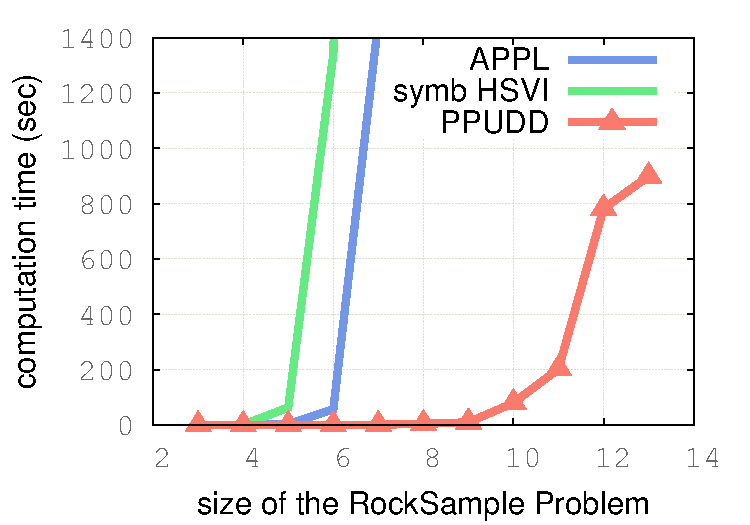
\includegraphics[width=\linewidth]{RockSampleCompTime.pdf}
\caption{Computation time (sec)}
\label{figureRS1}
\end{subfigure}
\begin{subfigure}[c]{.48\linewidth}
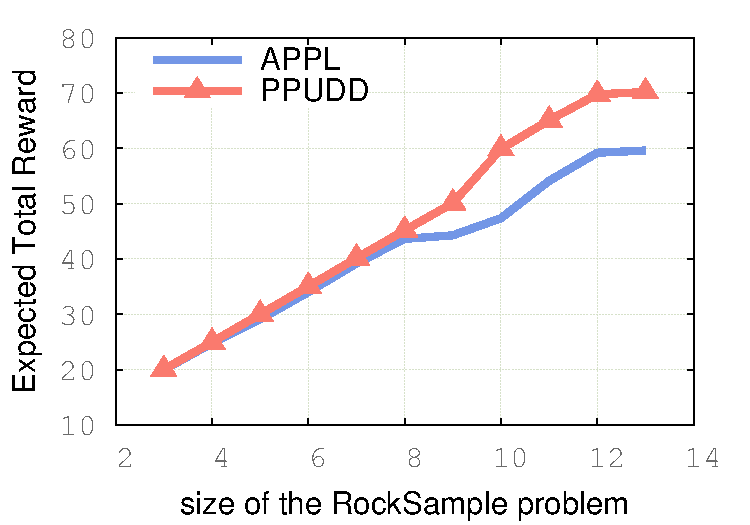
\includegraphics[width=\linewidth]{courbePerfTime.pdf}
\caption{Expected total reward}
\label{figureRS2}
\end{subfigure}
\vspace{0.5cm}
\caption[PPUDD vs. APPL and symb-HSVI, RockSample problem]{PPUDD vs. APPL and symb HSVI on the RockSample problem: the $x$-axis represents indexes of problem instances, increasing with the problem sizes.}
\end{figure}
Instead of precision, computation
time of APPL can be fixed at PPUDD's computation time in order to compare their
expected total rewards (using probabilistic model's rewards) 
after they consumed the same CPU time. 
%For PPUDD, we
%simply evaluated with the probabilistic model the policy that was computed
% under
%possibilistic settings.
Surprisingly, Figure \ref{figureRS2} shows that rewards gathered are higher with
PPUDD than with APPL. The reason is that APPL is in fact an approximate
probabilistic planner, which shows that our approach consisting in exactly
solving an approximate model can outperform algorithms that approximately solve
an exact model. 
Moreover, exact POMDP planners are
unable to scale to problems of the size of the RockSample ones.
Finally, it is worth noting that probabilities of the
observation model, which represent uncertainties of sensor outputs, may be
difficult to precisely know in practice, in which case possibilistic models may
be more physically accurate. 
In fact for this example the policy produced by
PPUDD is the best to get all possible rewards: this is essentially because the
rover can be sure of a rock's nature checking 
when it is on it.

These results assured us that it was not unreasonable to present PPUDD
in the International Probabilistic Planning Competition 2014,
even though the computation of strategies for probabilistic problems 
is not the initial vocation of this solver.
The next section describes the competition context
as well as the presented versions of PPUDD,
and discusses the results of the different competitor solvers.

\subsection{Comp�tition de planification probabiliste internationale 2014}
% TODO TODO TODO TODO 
% presentation de la compet 1
% presentation des competiteurs
% presentation de nos versions
% MASK, ATPPUDD, description 
% description des domains et en parallele, les resultats et commentaires
% + citer depot \\

%puis les 2 chaps suivants \\
%puis intro/concl \\


The fully observable track 
of the International Probabilistic Planning Competition (IPPC) 
allows to fairly compare performances of MDP solvers.
The competitors' solvers have to compute 
strategies for some problems 
which are not known in advance.
Given one of these problems, 
solvers have a limited amount of time 
to send actions to the competition server 
which simulates the evolution of the system state:
successive states are sampled by the competition server
using the transition probability 
distributions of the MDP defining the problem, 
and sent to a given competitor's solver.
For each system state received, the solver 
has to send back the action
it has computed.
These data exchanges are conducted 
during few trials of finite horizon and
the score of the solver for the considered problem 
is the average (over trials) 
of the undiscounted and finite sum of 
rewards along the trajectory generated by the trial.

Materials about this competition are available at the official web page of the competition
\url{https://cs.uwaterloo.ca/~mgrzes/IPPC_2014/}.
Problems are grouped in \textit{domains}, 
which are MDPs whose a finite number of parameters are undefined:
the problem, or MDP, used in practice during the competition
is an \textit{instance} of a domain, \textit{i.e.}
a domain whose parameters have been set.
In this competition, $8$ domains have been proposed,
called respectively
\textit{Academic advising}, \textit{Crossing traffic}, \textit{Elevators}, 
\textit{Skill teaching}, \textit{Tamarisk}, \textit{Traffic}, \textit{Triangle tireworld}
and \textit{Wildfire}.
Three possible encodings of the instances of these domains are proposed,
\textit{i.e.} three different languages can be used to describe the instances:
the first is the \textit{Planning Domain Definition Language} (PPDDL, \cite{Younes_ppddl1.0});
the second is a \textit{LISP}-like language introduced with symbolic algorithms such as SPUDD 
which defines explicitely transition probability distributions and reward function as ADDs
(see \url{http://users.cecs.anu.edu.au/~ssanner/IPPC_2011/}); 
finally, the third is the \textit{Relational Dynamic Influence Diagram Language} (RDDL, \cite{Sanner_relationaldynamic})
which is simpler and more expressive than the previous ones.
The competition consists in evaluating the solver over 
$10$ instances per domain with $30$ runs per instance and
$18$ minutes per instance: it takes $24$ hours in total.

In order to ensure that everyone has the same computational power,
each competitor solver is set up in a remote server whose RAM is $7.5$Gb 
with $2$ cores.% (``m3.large'', see \url{https://aws.amazon.com/ec2/pricing/}).
The client and server for the competition are available in the open source \textit{RDDLSim} software, 
which is available online at \url{http://code.google.com/p/rddlsim/}.
Four solvers have been proposed for this competition:
\begin{itemize}
\item \textit{PROST} \cite{DBLP:conf/aips/KellerE12}, based on \textit{Upper Confidence bound applied to Trees} (UCT, \cite{Kocsis:2006:BBM:2091602.2091633})
and using directly RDDL encoding;
\item \textit{GOURMAND} \cite{DBLP:conf/aaai/KolobovMW12,Kolobov12reverseiterative}, based on \textit{Labeled Real Time Dynamic Programming} (LRTDP, \cite{Bonet03labeledrtdp})
using PPDDL encoding;
\item \textit{symbolic LRTDP}, using ADDs and LISP-like encoding \cite{symbLRTDP};
\item our algorithm PPUDD, using LISP-like encoding too.
\end{itemize}

As the score given to solvers only depends on the $40$ first stages of the process,
the presented version of PPUDD consists of the Algorithm \ref{PPUDD} 
with the ``while condition'' $\overline{U^*} \neq \overline{U^c}$ at line \ref{while_PPUDD}
replaced by the condition ``iteration $\leqslant 40$''.
It also incrementally augments the planning
horizon while maintaining a mask stored in form of 
a Binary Decision Diagram (BDD, \textit{i.e.} an ADD with leaves in $\set{0,1}$) 
representing the states reachable from the initial state:
the computation of the current value function is then restricted
to the reachable states only. While PPUDD is an offline algorithm,
we proposed also \textit{AnyTime PPUDD} (ATPPUDD) 
which is an anytime version which learns computation times of
Bellman backups while dispatching the computational effort accordingly
over the remaining planning horizon much like GOURMAND does in the
probabilistic world (see \cite{DBLP:conf/aaai/KolobovMW12}). 

When encoded with the LISP-like format, 
problems of the competition, \textit{i.e.} instances of each domains, 
are described as factored MDPs
with boolean system state variables: 
for each action $a \in \mathcal{A}$ and for each next boolean system state variable $X_i'$, 
one ADD representing the corresponding transition probability distribution
$\textbf{p} \Big( X_i' \ \Big\vert \ parents(X_i'), a \Big)$ is given.
In order to define the $\pi$-MDP which will be solved by PPUDD,
we simply normalize these distributions in the possibilistic sense:
we set to $1$ the possibility degree of an assignment of $X_i'$ when 
its probability value is maximal, and to the probability value otherwise.
For instance, for a given assignment of the previous variables $parents(X_i')$, 
if the probability value of the assignment (or event) $X_i'=1$ is $0.7$ 
(and thus probability $0.3$ that $X_i' = 0$), 
then the possibility degree of $X_i'=1$ is set to $1$,
and the one of $X_i' = 0$ is set to $0.3$.

In terms of ADDs, it can be computed as follows:
let us first recall the notation  $\textbf{p} \Big( X_i' \ \Big\vert \ parents(X_i'),a \Big)^{X_i'=0}$,
used to represent the subtree of the ADD
$\textbf{p} \Big( X_i' \ \Big\vert \ parents(X_i'),a \Big)$ setting $X_i'$ to false (\textit{i.e.} to $0$).
As well, $\textbf{p} \Big( X_i' \ \Big\vert \ parents(X_i'),a \Big)^{X_i'=1}$ is the subtree of the same ADD, setting $X_i'$ to true (\textit{i.e.} to $1$).
Let us denote by $\mathds{1}_{\textbf{p}_{\top}>\textbf{p}_{\bot}}$ 
the BDD equal to $1$ for each variable assignment such that %$X_i'$ is true ($X_i'=\top$),
%and $0$ otherwise. 
%for each assignment of the variables of $parents(X_i')$ such that 
%\ovalbox{$\min$}
\[ \textbf{p} \Big( X_i' \ \Big\vert \ parents(X_i'),a \Big)^{X_i'=0} < \textbf{p} \Big( X_i' \ \Big\vert \ parents(X_i'),a \Big)^{X_i'=1}, \]
and equal to $0$ for other assignments.
The BDD always equal to $1$ is denoted by $\mathds{1}$. 
The BDD $\mathds{1}_{\textbf{p}=0.5}$ is equal to $1$
for variable assignments such that the probability of the event $X_i'=1$ (or $X_i'=0$) 
is equal to $0.5$, and this BDD is equal to $0$ otherwise.
We can also denote by
$\mathds{1}_{\textbf{p}_{\top}<\textbf{p}_{\bot}} $
the BDD which is equal to $1$ for assignments of variables in $parents(X_i')$ 
such that the probability of event $X_i' = 1$
is lower than the probability of event $X_i'=0$:
this BDD can be computed from previous BDDs,
$ \mathds{1} \ \ovalbox{$-$} \ \mathds{1}_{\textbf{p}_{\top}>\textbf{p}_{\bot}} \ \ovalbox{$-$} \ \mathds{1}_{\textbf{p}=0.5}$,
where $\ovalbox{$-$}$ is the minus operator, applied to trees.
The possibility transition distribution for the $i^{th}$ variable is
\begin{eqnarray*}
\pi \Big( X_i' \ \Big\vert \ parents(X_i'),a \Big) = \ovalbox{$\max$} \Bigg\{ 	& \mathds{1}_{\textbf{p}=0.5}, 														& \\
				& \ovalbox{$\min$} \bigg\{ \mathds{1}_{\textbf{p}_{\top}>\textbf{p}_{\bot}}, \textbf{p} \Big( X_i' \Big\vert parents(X_i'), a \Big) \bigg\} , 	& \\
				& \ovalbox{$\min$} \bigg\{ \mathds{1}_{\textbf{p}_{\top}<\textbf{p}_{\bot}}  , \textbf{p} \Big( X_i' \Big\vert parents(X_i'), a \Big) \bigg\} 	& 	\Bigg\} 
\end{eqnarray*}

As well, for each action $a \in \mathcal{A}$, 
an ADD representing the reward function for this action 
is provided and denoted by $r(X_1,\ldots,X_n,a)$. 
Let us define then for each $s \in \mathcal{S}$ and $a \in \mathcal{A}$,
\[ \Psi(s,a) = \frac{ r(s,a) - \min_{s,a} r(s,a) }{ \max_{s,a} r(s,a) - \min_{s,a} r(s,a)} \in [0,1]. \]
The terminal preference function is set to $\Psi(s) = \max_{a \in \mathcal{A}} \Psi(s,a)$,
and the strategy is initialized by $\delta^*(s) \in \operatorname*{argmax}_{a \in \mathcal{A}} \Psi(s,a)$
at the beginning of the algorithm.

Note that possibility and preference degrees are not in a scale $\mathcal{L}$ 
as previously defined (\textit{i.e.} $\set{ 0, \frac{1}{k}, \frac{2}{k} \ldots, 1 }$ for some $k \geqslant1$).
Indeed, possibility degrees comes from probability values, 
and preferences are normalized rewards.
However, only $\max$ and $\min$ operators are used, 
so it has no impact on the qualitative results of the computations. 

The library used to perform computations with ADDs
is the \textit{CU Decision Diagram Package} 
(CUDD, \url{http://vlsi.colorado.edu/~fabio/CUDD/}),
and the described versions of PPUDD are available 
at the adress \url{https://github.com/drougui/ppudd}.

Following figures illustrates the results of IPPC 2014:
the score is given in function of the instance index,
which generally increases with the difficulty (or the size) 
of the associated problem.

\begin{figure} \centering
\definecolor{ggreen}{rgb}{0.3,0.7,0.4}
\begin{tikzpicture}
\begin{axis}[grid=major,xmin=1,xmax=10,xtick={1,2,3,4,5,6,7,8,9,10},
legend entries={GOURMAND, PROST, Symbolic LRTDP, random strategy, ``noop'' strategy, ATPPUDD, PPUDD},legend style={at={(1.52,1.1)}},
xlabel={Problem instances},
ylabel={Raw average score},
title={\textit{Academic advising} problem},width=11cm,height=11cm]
\addplot+[line width=1pt] plot[error bars/.cd,y dir=both,y explicit] table[x index=1, y index=5, y error index=6]{IPPC14_resultats/academic_advising.txt};%GOURMAND
\addplot+[line width=1pt] plot[error bars/.cd,y dir=both,y explicit] table[x index=1, y index=26, y error index=27]{IPPC14_resultats/academic_advising.txt};%PROST14
\addplot+[line width=1pt] plot[error bars/.cd,y dir=both,y explicit] table[x index=1, y index=40, y error index=41]{IPPC14_resultats/academic_advising.txt};%FACTOREDLRTDP
\addplot+[line width=1pt] plot[error bars/.cd,y dir=both,y explicit] table[x index=1, y index=33, y error index=34]{IPPC14_resultats/academic_advising.txt};%RANDOM
\addplot+[color=black,line width=1pt] plot[error bars/.cd,y dir=both,y explicit] table[x index=1, y index=12, y error index=13]{IPPC14_resultats/academic_advising.txt};%NOOP
\addplot[color=ggreen,mark=diamond,line width=3.2pt] plot[error bars/.cd,y dir=both,y explicit] table[x index=1, y index=54, y error index=55]{IPPC14_resultats/academic_advising.txt};%ATPPUDD 
\addplot[color=orange,mark=diamond,line width=2.2pt] plot[error bars/.cd,y dir=both,y explicit] table[x index=1, y index=47, y error index=48]{IPPC14_resultats/academic_advising.txt};%PPUDD 
\end{axis}
\end{tikzpicture}
\\
\vspace{0.5cm}
\begin{tikzpicture}
\begin{axis}[grid=major,xmin=1,xmax=10,xtick={1,2,3,4,5,6,7,8,9,10},
xlabel={Problem instances},
ylabel={Raw average score},
title={\textit{Crossing traffic} problem},width=11cm,height=11cm]
\addplot+[line width=1pt] plot[error bars/.cd,y dir=both,y explicit] table[x index=1, y index=5, y error index=6]{IPPC14_resultats/crossing_traffic_inst_mdp.txt};%GOURMAND
\addplot+[line width=1pt] plot[error bars/.cd,y dir=both,y explicit] table[x index=1, y index=26, y error index=27]{IPPC14_resultats/crossing_traffic_inst_mdp.txt};%PROST14
\addplot+[line width=1pt] plot[error bars/.cd,y dir=both,y explicit] table[x index=1, y index=40, y error index=41]{IPPC14_resultats/crossing_traffic_inst_mdp.txt};%FACTOREDLRTDP
\addplot+[line width=1pt] plot[error bars/.cd,y dir=both,y explicit] table[x index=1, y index=33, y error index=34]{IPPC14_resultats/crossing_traffic_inst_mdp.txt};%RANDOM
\addplot+[color=black,line width=1pt] plot[error bars/.cd,y dir=both,y explicit] table[x index=1, y index=12, y error index=13]{IPPC14_resultats/crossing_traffic_inst_mdp.txt};%NOOP
\addplot[color=ggreen,mark=diamond,line width=3.2pt] plot[error bars/.cd,y dir=both,y explicit] table[x index=1, y index=54, y error index=55]{IPPC14_resultats/crossing_traffic_inst_mdp.txt};%ATPPUDD 
\addplot[color=orange,mark=diamond,line width=2.2pt] plot[error bars/.cd,y dir=both,y explicit] table[x index=1, y index=47, y error index=48]{IPPC14_resultats/crossing_traffic_inst_mdp.txt};%PPUDD 
\end{axis}
\end{tikzpicture}
\caption[Results of IPPC 2014: \textit{Academic advising} and \textit{Crossing traffic} problems]{
Results of the International Probabilistic Planning Competition -- Fully Observable track}
\label{figure_IPPC_ACA_CRO}
\end{figure}

Figure \ref{figure_IPPC_ACA_CRO} presents the scores obtained by each solver 
for each of the $10$ instances of the \textit{Academic advising} domains,
\textit{i.e.} the average over $30$ trials of the sum of the encountered rewards.
Performances of our algorithms are close to the best ones.
However, an unexplained and unwanted bug occurred with ATPPUDD for the $2^{nd}$ instance, 
as only $3$ runs have been performed by this solver.
For the other instances, PPUDD and ATPPUDD produce strategies with performances like 
PROST and GOURMAND, and better than Symbolic LRTDP.
This has been less true for the \textit{Crossing traffic} problem, 
whose results are also described by Figure \ref{figure_IPPC_ACA_CRO}.
This problem models a robot which has to reach a goal 
which is across an highway with a lot of cars.
These cars arrive randomly and move left.
As the possibility degree of the fact that no car arrive 
is set to $1$ by our naive MDP to $\pi$-MDP translation,
the optimistic criterion leads to decide to cross the street,
even if an unseen car may arrive (with a probability $<0.5$ but bit enough to be cautious). 
This explain the poor quality of the produced strategies 
for this domain. Note however that, for the $6$ last instances (most difficult problems)
our approach leads to better strategies than the probabilistic solver Symbolic LRTDP.

\begin{figure} \centering
\definecolor{ggreen}{rgb}{0.3,0.7,0.4}
\begin{tikzpicture}
\begin{axis}[grid=major,xmin=1,xmax=10,xtick={1,2,3,4,5,6,7,8,9,10},
legend entries={GOURMAND, PROST, Symbolic LRTDP, random strategy, ``noop'' strategy, ATPPUDD, PPUDD},legend style={at={(1.52,1.1)}},width=11cm,height=11cm,
xlabel={Problem instances},
ylabel={Raw average score},
title={\textit{Elevators} problem}]
\addplot+[line width=1pt] plot[error bars/.cd,y dir=both,y explicit] table[x index=1, y index=5, y error index=6]{IPPC14_resultats/elevators_inst_mdp.txt};%GOURMAND
\addplot+[line width=1pt] plot[error bars/.cd,y dir=both,y explicit] table[x index=1, y index=26, y error index=27]{IPPC14_resultats/elevators_inst_mdp.txt};%PROST14
\addplot+[line width=1pt] plot[error bars/.cd,y dir=both,y explicit] table[x index=1, y index=40, y error index=41]{IPPC14_resultats/elevators_inst_mdp.txt};%FACTOREDLRTDP
\addplot+[line width=1pt] plot[error bars/.cd,y dir=both,y explicit] table[x index=1, y index=33, y error index=34]{IPPC14_resultats/elevators_inst_mdp.txt};%RANDOM
\addplot+[color=black,line width=1pt] plot[error bars/.cd,y dir=both,y explicit] table[x index=1, y index=12, y error index=13]{IPPC14_resultats/elevators_inst_mdp.txt};%NOOP
\addplot[color=ggreen,mark=diamond,line width=3.2pt] plot[error bars/.cd,y dir=both,y explicit] table[x index=1, y index=54, y error index=55]{IPPC14_resultats/elevators_inst_mdp.txt};%ATPPUDD 
\addplot[color=orange,mark=diamond,line width=2.2pt] plot[error bars/.cd,y dir=both,y explicit] table[x index=1, y index=47, y error index=48]{IPPC14_resultats/elevators_inst_mdp.txt};%PPUDD 
\end{axis}
\end{tikzpicture}
\\
\vspace{0.5cm}
\begin{tikzpicture}
\begin{axis}[grid=major,xmin=1,xmax=10,xtick={1,2,3,4,5,6,7,8,9,10},
xlabel={Problem instances},
ylabel={Raw average score},
title={\textit{Skill teaching} problem},width=11cm,height=11cm]
\addplot+[line width=1pt] plot[error bars/.cd,y dir=both,y explicit] table[x index=1, y index=5, y error index=6]{IPPC14_resultats/skill_teaching_inst_mdp.txt};%GOURMAND
\addplot+[line width=1pt] plot[error bars/.cd,y dir=both,y explicit] table[x index=1, y index=26, y error index=27]{IPPC14_resultats/skill_teaching_inst_mdp.txt};%PROST14
\addplot+[line width=1pt] plot[error bars/.cd,y dir=both,y explicit] table[x index=1, y index=40, y error index=41]{IPPC14_resultats/skill_teaching_inst_mdp.txt};%FACTOREDLRTDP
\addplot+[line width=1pt] plot[error bars/.cd,y dir=both,y explicit] table[x index=1, y index=33, y error index=34]{IPPC14_resultats/skill_teaching_inst_mdp.txt};%RANDOM
\addplot+[color=black,line width=1pt] plot[error bars/.cd,y dir=both,y explicit] table[x index=1, y index=12, y error index=13]{IPPC14_resultats/skill_teaching_inst_mdp.txt};%NOOP
\addplot[color=ggreen,mark=diamond,line width=3.2pt] plot[error bars/.cd,y dir=both,y explicit] table[x index=1, y index=54, y error index=55]{IPPC14_resultats/skill_teaching_inst_mdp.txt};%ATPPUDD 
\addplot[color=orange,mark=diamond,line width=2.2pt] plot[error bars/.cd,y dir=both,y explicit] table[x index=1, y index=47, y error index=48]{IPPC14_resultats/skill_teaching_inst_mdp.txt};%PPUDD 
\end{axis}
\end{tikzpicture}
\caption[Results of IPPC 2014: \textit{Elevators} and \textit{Skill teaching problems}]{
Results of the International Probabilistic Planning Competition -- Fully Observable track}
\label{figure_IPPC_ELE_SKI}
\end{figure}

In the \textit{Elevators} problem, people arrive randomly and have to be transported 
to the correct building stage: 
as the frequentist information is lost using the possibilistic approach
and seems important in this problem (people do not want to wait once arrived), 
scores of our algorithms are poorer than the ones of PROST and GOURMAND.
The toy example at the beginning of the introduction of this chapter
illustrates that the possibilistic approaches can select actions probabilistically clearly suboptimal
when the probability values are at the heart of the problem.
PPUDD and ATPPUDD are however better than Symbolic LRTDP, as shown by Figure \ref{figure_IPPC_ELE_SKI},
and than doing nothing (``noop strategy'') or choosing actions randomly (``random strategy'').
PPUDD and ATPPUDD have quite good behaviours with the \textit{Skill teaching} problem 
as illustrated by the same figure. Moreover, ATPPUDD leads to better results
for the last three instances: as these instances are the \textit{Skill teaching} problems 
with the largest system space,  
the anytime version, which manages the computation time, 
produces strategies with better performances
than PPUDD, which classically solve the associated $\pi$-MDP, 
but cannot complete computations and lead to a poorer strategy.

\begin{figure} \centering
\definecolor{ggreen}{rgb}{0.3,0.7,0.4}
\begin{tikzpicture}
\begin{axis}[grid=major,xmin=1,xmax=10,xtick={1,2,3,4,5,6,7,8,9,10},
xlabel={Problem instances},
ylabel={Raw average score},
title={\textit{Tamarisk} problem},
compat=newest,
legend entries={GOURMAND, PROST, Symbolic LRTDP, random strategy, ``noop'' strategy, ATPPUDD, PPUDD},legend style={at={(1.52,1.1)}},width=11cm,height=11cm]
\addplot+[line width=1pt] plot[error bars/.cd,y dir=both,y explicit] table[x index=1, y index=5, y error index=6]{IPPC14_resultats/tamarisk.txt};%GOURMAND
\addplot+[line width=1pt] plot[error bars/.cd,y dir=both,y explicit] table[x index=1, y index=26, y error index=27]{IPPC14_resultats/tamarisk.txt};%PROST14
\addplot+[line width=1pt] plot[error bars/.cd,y dir=both,y explicit] table[x index=1, y index=40, y error index=41]{IPPC14_resultats/tamarisk.txt};%FACTOREDLRTDP
\addplot+[line width=1pt] plot[error bars/.cd,y dir=both,y explicit] table[x index=1, y index=33, y error index=34]{IPPC14_resultats/tamarisk.txt};%RANDOM
\addplot+[color=black,line width=1pt] plot[error bars/.cd,y dir=both,y explicit] table[x index=1, y index=12, y error index=13]{IPPC14_resultats/tamarisk.txt};%NOOP
\addplot[color=ggreen,mark=diamond,line width=3.2pt] plot[error bars/.cd,y dir=both,y explicit] table[x index=1, y index=54, y error index=55]{IPPC14_resultats/tamarisk.txt};%ATPPUDD 
\addplot[color=orange,mark=diamond,line width=2.2pt] plot[error bars/.cd,y dir=both,y explicit] table[x index=1, y index=47, y error index=48]{IPPC14_resultats/tamarisk.txt};%PPUDD 
\end{axis}
\end{tikzpicture}
\\
\vspace{0.5cm}
\begin{tikzpicture}
\begin{axis}[grid=major,xmin=1,xmax=10,xtick={1,2,3,4,5,6,7,8,9,10},
xlabel={Problem instances},
ylabel={Raw average score},
title={\textit{Traffic} problem},
width=11cm,height=11cm]
\addplot+[line width=1pt] plot[error bars/.cd,y dir=both,y explicit] table[x index=1, y index=5, y error index=6]{IPPC14_resultats/traffic_inst_mdp.txt};%GOURMAND
\addplot+[line width=1pt] plot[error bars/.cd,y dir=both,y explicit] table[x index=1, y index=26, y error index=27]{IPPC14_resultats/traffic_inst_mdp.txt};%PROST14
\addplot+[line width=1pt] plot[error bars/.cd,y dir=both,y explicit] table[x index=1, y index=40, y error index=41]{IPPC14_resultats/traffic_inst_mdp.txt};%FACTOREDLRTDP
\addplot+[line width=1pt] plot[error bars/.cd,y dir=both,y explicit] table[x index=1, y index=33, y error index=34]{IPPC14_resultats/traffic_inst_mdp.txt};%RANDOM
\addplot+[color=black,line width=1pt] plot[error bars/.cd,y dir=both,y explicit] table[x index=1, y index=12, y error index=13]{IPPC14_resultats/traffic_inst_mdp.txt};%NOOP
\addplot[color=ggreen,mark=diamond,line width=3.2pt] plot[error bars/.cd,y dir=both,y explicit] table[x index=1, y index=54, y error index=55]{IPPC14_resultats/traffic_inst_mdp.txt};%ATPPUDD 
\addplot[color=orange,mark=diamond,line width=2.2pt] plot[error bars/.cd,y dir=both,y explicit] table[x index=1, y index=47, y error index=48]{IPPC14_resultats/traffic_inst_mdp.txt};%PPUDD 
\end{axis}
\end{tikzpicture}
\caption[Results of IPPC 2014: \textit{Tamarisk} and \textit{Traffic} problems]{
Results of the International Probabilistic Planning Competition -- Fully Observable track}
\label{figure_IPPC_TAM_TRA}
\end{figure}


With respect to other solvers, possibilistic solvers have good results 
with the \textit{Tamarisk} domain, as shown in Figure \ref{figure_IPPC_TAM_TRA}..
However, some instances (e.g. the $6^{th}$, the $8^{th}$ and the $10^{th}$) 
are not even run as the ADD instantiation takes too long. 
Symbolic LRTP faces the same issue
as it uses also the LISP-like encoding of the problem.
We think that this is an issue specific to the competition,
as each problem has to be equivalently translated into
three different languages (RDDL, PPDDL and LISP-like),
which produces sometimes artificially complex
encodings of the problems.
The \textit{Traffic} domain is really hard to solve by PPUDD and ATPPUDD (see Figure \ref{figure_IPPC_TAM_TRA}). 
Actually the least scores are obtained with this domain,
and even the random and the noop strategies are better strategies.
Note that we did not implement any ``watchdog''
returning random actions when the computed strategy is less effective than the random one.
However, this kind of gadget is essential to improve results for such large and risky problem. 
As mentioned above for the \textit{Crossing traffic} problem, 
the optimistic criterion may lead to dangerous actions, as it does here.
Moreover, as this problem involves frequentist information (car arrivals)
an high suboptimality of the strategy produced by the possibilistic approach
is confirmed for this kind of problems (see the \textit{Elevator} problems). 
Finally, the \textit{Traffic} problem is known to be one of the hardest domain,
so ADD instantiation takes long, as well as computations, 
which are then not proceeded enough to produce satisfying results. 

\begin{figure} \centering
\definecolor{ggreen}{rgb}{0.3,0.7,0.4}
\begin{tikzpicture}
\begin{axis}[grid=major,xmin=1,xmax=10,xtick={1,2,3,4,5,6,7,8,9,10},
legend entries={GOURMAND, PROST, Symbolic LRTDP, random strategy, ``noop'' strategy, ATPPUDD, PPUDD},legend style={at={(1.52,1.1)}},width=11cm,height=11cm,
xlabel={Problem instances},
ylabel={Raw average score},
title={\textit{Triangle tireworld} problem}]
\addplot+[line width=1pt] plot[error bars/.cd,y dir=both,y explicit] table[x index=1, y index=5, y error index=6]{IPPC14_resultats/triangle_tireworld_inst_mdp.txt};%GOURMAND
\addplot+[line width=1pt] plot[error bars/.cd,y dir=both,y explicit] table[x index=1, y index=26, y error index=27]{IPPC14_resultats/triangle_tireworld_inst_mdp.txt};%PROST14
\addplot+[line width=1pt] plot[error bars/.cd,y dir=both,y explicit] table[x index=1, y index=40, y error index=41]{IPPC14_resultats/triangle_tireworld_inst_mdp.txt};%FACTOREDLRTDP
\addplot+[line width=1pt] plot[error bars/.cd,y dir=both,y explicit] table[x index=1, y index=33, y error index=34]{IPPC14_resultats/triangle_tireworld_inst_mdp.txt};%RANDOM
\addplot+[color=black,line width=1pt] plot[error bars/.cd,y dir=both,y explicit] table[x index=1, y index=12, y error index=13]{IPPC14_resultats/triangle_tireworld_inst_mdp.txt};%NOOP
\addplot[color=ggreen,mark=diamond,line width=3.2pt] plot[error bars/.cd,y dir=both,y explicit] table[x index=1, y index=54, y error index=55]{IPPC14_resultats/triangle_tireworld_inst_mdp.txt};%ATPPUDD 
\addplot[color=orange,mark=diamond,line width=2.2pt] plot[error bars/.cd,y dir=both,y explicit] table[x index=1, y index=47, y error index=48]{IPPC14_resultats/triangle_tireworld_inst_mdp.txt};%PPUDD
\end{axis}
\end{tikzpicture}
\\
\vspace{0.5cm}
\begin{tikzpicture}
\begin{axis}[grid=major,xmin=1,xmax=10,xtick={1,2,3,4,5,6,7,8,9,10}, width=11cm,height=11cm,
xlabel={Problem instances},
ylabel={Raw average score},
title={\textit{Wildfire} problem}]
\addplot+[line width=1pt] plot[error bars/.cd,y dir=both,y explicit] table[x index=1, y index=5, y error index=6]{IPPC14_resultats/wildfire_inst_mdp.txt};%GOURMAND
\addplot+[line width=1pt] plot[error bars/.cd,y dir=both,y explicit] table[x index=1, y index=26, y error index=27]{IPPC14_resultats/wildfire_inst_mdp.txt};%PROST14
\addplot+[line width=1pt] plot[error bars/.cd,y dir=both,y explicit] table[x index=1, y index=40, y error index=41]{IPPC14_resultats/wildfire_inst_mdp.txt};%FACTOREDLRTDP
\addplot+[line width=1pt] plot[error bars/.cd,y dir=both,y explicit] table[x index=1, y index=33, y error index=34]{IPPC14_resultats/wildfire_inst_mdp.txt};%RANDOM
\addplot+[color=black,line width=1pt] plot[error bars/.cd,y dir=both,y explicit] table[x index=1, y index=12, y error index=13]{IPPC14_resultats/wildfire_inst_mdp.txt};%NOOP
\addplot[color=ggreen,mark=diamond,line width=3.2pt] plot[error bars/.cd,y dir=both,y explicit] table[x index=1, y index=54, y error index=55]{IPPC14_resultats/wildfire_inst_mdp.txt};%ATPPUDD 
\addplot[color=orange,mark=diamond,line width=2.2pt] plot[error bars/.cd,y dir=both,y explicit] table[x index=1, y index=47, y error index=48]{IPPC14_resultats/wildfire_inst_mdp.txt};%PPUDD 
\end{axis}
\end{tikzpicture}
\caption[Results of IPPC 2014: \textit{Triangle tireworld} and \textit{Wildfire} problems]{
Results of the International Probabilistic Planning Competition -- Fully Observable track}
\label{figure_IPPC_TRI_WIL}
\end{figure}

Finally, the two last domains, whose results are described in Figure \ref{figure_IPPC_TRI_WIL},
are called \textit{Triangle Tireworld} and \textit{Wildfire}.
Firt, ATPPUDD faces an unexplained bug for each instance of the \textit{Triangle Tireworld} domain:
no trial is performed from the $5^{th}$ instance, and maximum $2$ trials are performed for other instances
(which explains the poor score for each instance).
As already mentioned for the \textit{Tamarisk} domain, 
ADD instantiation takes too long for the last instances,
and no trial is performed for the last $4$ instances 
with PPUDD too: Symbolic LRTDP faces the same issue. 
The last domain, called \textit{Wildfire}, leads to highly frequentist problems:
it involves random fire starts. 
That is why PPUDD and ATPPUDD strategies are not really efficient, 
but not too distant from Symbolic LRTDP solver's results.

%%%% TODO TODO TODO TODO TODO TODO TODO TODO TODO TODO TODO TODO
%%%% TODO TODO TODO TODO TODO TODO TODO TODO TODO TODO TODO TODO
%%%% TODO TODO TODO TODO TODO TODO TODO TODO TODO TODO TODO TODO
%%%% TODO TODO TODO TODO TODO TODO TODO TODO TODO TODO TODO TODO
%\section{Practical Implementation of the Algorithms using ADDs}
%CUDD library
%%%% TODO TODO TODO TODO TODO TODO TODO TODO TODO TODO TODO TODO
%%%% TODO TODO TODO TODO TODO TODO TODO TODO TODO TODO TODO TODO
%%%% TODO TODO TODO TODO TODO TODO TODO TODO TODO TODO TODO TODO
%%%% TODO TODO TODO TODO TODO TODO TODO TODO TODO TODO TODO TODO


\section{Conclusion} 
We presented PPUDD, the first algorithm to the best of our knowledge that 
solves factored possibilistic qualitative (MO)MDPs with symbolic calculations. In our opinion,
possibilistic models are a good tradeoff between non-deterministic ones, whose
uncertainties are not at all quantified yielding a very approximate model, and
probabilistic ones, where uncertainties are fully specified,
sometimes arbitrarily in practice. 
The resolution of planning problems 
using the framework of non-determinism 
is called \textit{contingent/conformant planning} 
studied for instance in \cite{Albore_atranslation-based,bonet2014flexible}.
By the way, in the introduction of this thesis,
we might also add ``non-determinism''
as a particular case of Possibility Theory
in Figure \ref{uncertainty_theories},
as values of associated non additive measures
are $0$ or $1$ instead of a more flexible scale $\mathcal{L}$.

Moreover,
$\pi$-MOMDPs reason about finite values in a qualitative scale $\mathcal{L}$ whereas
probabilistic MOMDPs deal with values in $\mathbb{R}$, which implies larger ADDs
for symbolic algorithms. Also, the former reduce to finite-state belief
$\pi$-MDPs contrary to the latter that yield \emph{continuous}-state belief MDPs
of significantly higher complexity. Our experimental results highlight the point that using an
exact algorithm (PPUDD) for an approximate model ($\pi$-MDPs) can bring significantly faster computations
than reasoning about complex exact models, while providing better
strategies than approximate algorithms (APPL) for exact models. 
In the future, we would like to developp a probabilistic algorithm using 
the generalization of our possibilistic belief factorization theory to
probabilistic settings (see Theorem \ref{thm_factoredPROBbelief}): 
related but sightly different results have been proposed for
probabilistic POMDPs \cite{DBLP:conf/aips/ShaniPBS08,Poupart:2005:phd}. 
These results also does not concern 
the case of mixed observability.

This chapter finally presents the results of our possibilistic approach
during IPPC 2014: 
the highlighted bottleneck of our possibilistic algorithms
resides on the translation from probabilities to possibilities: 
the naive automated translation presented before the description of the results 
leads to poor policies in benchmarks with complex dynamics and reward structures.
Another issue is the size of the input LISP-like encoded domains whose ADD
instantiation before optimization takes a very long time or 
does not even fit into memory for many difficult benchmarks:
this difficulty is shared with the Symbolic LRTDP solver.
However, there is almost no discretization of the initial probability values defining the MDP
in order to produce the possibility degrees
during the instantiation of the ADD defining the $\pi$-MDP:
the maximal difference between two possibility degrees is set to $10^{-3}$.
Stronger discretizations have not been tested yet, 
and could improve scores of our solvers for problems with such memory issues.
Modeling issues have been also highlighted, 
namely the fact that some problems request 
a cautious behaviour, not provided by the use of
the optimistic criterion (see Definition \ref{probstylerewrittenMOMDPcrit}) 
used during the competition. 
Moreover, as illustrated in introduction, 
these experiments show that problems with high entropy events 
are outperformed by probabilistic approaches since the possibilistic 
approach does not take into account the frequentist information about the problem.
The use of \textit{lexi}-approaches, as used in the following chapter, 
may be a possibilistic stratagem to get around this issue.
Note finally that the partially observable version of PPUDD 
(with the generation of a mask of reachable belief states, avoiding useless computations
on unreachable beliefs) is also available on the repository \url{https://github.com/drougui/ppudd}.

The next chapter, Chapter \ref{chap_IHM}, deals with \textit{Human-Machine Interaction} (HMI)
problems: the uncertainty dynamics of the system are in this context typically not known in terms
of probability values, and the qualitative possibilistic approach is shown to be a natural approach
to produce efficient diagnosis of human errors.

Finally, the last chapter, Chapter \ref{chap_hybrid},
takes into account the remarks made using the results of IPPC14:
an approach using Probability and Possibility Theory
in order to benefit from both approaches in the resolution of factored POMDPs
is presented: quantitative information of the problem is kept to avoid the highlighted modeling issues,
and the belief state is handled in a possibilistic way, in order to get a smart discretization of it
and to benefit from a finite and factorized belief state spaces.
This approach leads to a factored probabilistic MDP 
which can be solved for instance by GOURMAND or PROST
(which does not use the memory constraining LISP-like encoding).


% ============================================================
% 
\chapter{Application des Processus de Markov Cach�s pour le Diagnostic dans l'Int\'eraction Homme-Machine}
%%%%%%%%%%%%%%%%%%%%%%%%%%%%%%%%%%%%%%%%%%%%%%%%%%%%%%%%%%%%%%%%%%%%%%%
% TODO TODO TODO TODO TODO TODO TODO TODO TODO TODO TODO TODO TODO TODO
%%%%%%%%%%%%%%%%%%%%%%%%%%%%%%%%%%%%%%%%%%%%%%%%%%%%%%%%%%%%%%%%%%%%%%%
\label{chap_IHM}
%The work developed in this chapter is quite independent 
from the main theme of this thesis, namely the problem of
\textit{Decision Making under Uncertainty}.
This work, performed in collaboration with Sergio Pizziol
and extending the work of his PhD thesis \cite{SERGIOTHESIS}, 
contributes to modelling human-machine interactions.
It is part of this thesis since it is a significant example of 
the need of qualitative models (such as those presented in previous chapters)
in some practical situations.

We formalize here a framework providing an estimate 
of the human assessment of the machine state, 
an automated detection of human operator attentional errors, 
and finally an estimate of the most plausible causes of these errors.
A qualitative possibilistic approach is used to deal 
with uncertainty about the human operator assessment. 

The human-machine context is first introduced to point out the need 
for a new modelling method for human attentional error.
Then a human error model is derived from the machine logic, using expert assumptions on human errors and their plausibility.
A human-machine interaction model results from the combination of the machine logic and the error model.
Using the Possibility Theory, an analysis model estimating the human assessment 
is built on the interaction model, summed up in a \textit{Possibilistic Hidden Markov Processes} ($\pi$-HMPs).
The possibilistic analysis is first performed on a toy example. 
Finally the soundness of the approach is shown through simulation tests 
with pilots performing a flight mission.

% Note that keywords are not normally used for peerreview papers.
%Human-Machine Interaction, Possibility Theory, Human Assessment Estimation,
%Possibilistic Bayes Rule, Hidden Markov Process, Assessment Error Detection, Flight Simulation Tests.

\section{Introduction}
\label{intro}
In human-machine interaction studies, the problem of the 
correct human assessment of the machine state has been widely discussed. 
The main issue is that a human operator with a wrong assessment of the 
machine state is likely to perform {\em erroneous actions}, \textit{i.e.} 
actions whose outcome is different from what is intended \cite{Joshi03}. 

Many different approaches have been proposed to deal with this issue: 
among them, mental models and situation awareness \cite{Endsley95,rushby99}, 
formal inference rules \cite{Obrien09}, or {\em error models} for the human 
misinterpretation of the machine feedbacks \cite{rushby02a}. Those approaches 
are based on a deterministic model for the human error, suited for error 
dynamic analysis but not for error detection. Moreover, they do not benefit 
from the flexibility provided by uncertainty representations.

The human assessment of the machine state is not observable 
during the interaction with the machine: nevertheless it
may be estimated via uncertainty modelling for example using
Probability Theory \cite{Oaksford07}. However probability values 
can be difficult to define in practice 
because of a lack of quantitative information related to the human operator's 
behaviour. A method to build an interaction model 
relying on less informative data is needed. 
This chapter proposes a new method building such a model 
with qualitative expert data and using the machine logic.

The human assessment of the machine state (shortly {\em assessment}) is mainly 
based on the {\em feedbacks} provided by the machine. {\em Feedbacks} are pieces 
of information the machine sends (via visual or aural alerts/signs) in order 
to inform the human operator about its current state. Some formal approaches 
have been proposed in order to estimate whether the human receives enough 
feedbacks \cite{Ozveren90,combefis11}. Nevertheless even if enough feedbacks 
are provided, the problem of their correct reception remains. If the human does 
not perceive some machine feedbacks during the interaction, the human assessment may 
be incorrect, leading to erroneous actions based on such a wrong assessment: 
%The main objective 
%of this work is to formalise a model that provides an estimate of the assessment 
%based on 
%the actual machine state, on the feedbacks provided by the machine and on the 
%actions performed 
%by the human {\em i.e.} all the available inputs and outputs of the Human-Machine 
%interface.\\
the main objective of this work is to formalise an analysis model detecting 
assessment errors through human assessment estimation.\\

\begin{figure}
\centering
\begin{tikzpicture}[scale=1,transform shape]
%states
\tikzstyle{vertex}=[fill=black!20,draw=black, minimum size=20pt,line width=1pt,inner sep=5pt, minimum height=37pt]
\tikzstyle{vertexBIG}=[fill=black!20,draw=black, minimum width=280pt, minimum height=40pt,line width=1pt,inner sep=5pt]

\node[vertex] (M) at (-1,0) {\textbf{Machine}};
\node[vertex] (H) at (5,0) {\textbf{Human}};
\node[vertexBIG] (O) at (2,-2) {};
\node () at (1.7,-1.6) {\textbf{Observer}};
%\node[vertex] (H) at (0.4,-2.2) {Machine model};
%\node[vertex] (H) at (3.5,-2.2) {Human error model};

\node[ellipse,draw, thick,fill=blue!20] (el) at (-0.55,-2.2) {Machine model};
\node[ellipse,draw, thick,fill=blue!20] (el) at (4.15,-2.2) {Human error model};


\draw[->,>=latex,line width=2pt,color=red] (-0.15,0.3) -- (4.2,0.3);
\draw[->,>=latex,line width=2pt,color=red] (4.24,-0.3) -- (-0.15,-0.3);

\draw[->,>=latex,line width=1pt,color=red, dashed] (3.9,-0.3) -- (3.9,-1.3);
\draw[->,>=latex,line width=1pt,color=red, dashed] (1,0.3) -- (1,-1.3);

\node () at (1,0.6) {Feedbacks};
\node () at (3,-0.6) {Selections};
\end{tikzpicture}
\caption[Relation between actors involved in the Human-Machine Interation study]{The three actors involved in the study. The red arrows represent information flows.}
 \label{Observer}
\end{figure}

Three actors are involved in this framework: a machine, 
a human operator acting on the machine, 
and an observer analysing the human-machine interaction.
Human operator actions on the machine are called \textit{selections}.

The observer knows the machine logic and contemplates possible human 
assessment errors. Moreover, during the human machine interaction, 
it observes a sequence of data generated by the machine and the human operator: 
these data are called \textit{observable occurrences}, and consist 
in each successive feedback (from the machine) and selection 
(from the human operator), as illustrated Figure~\ref{Observer}. 
Machine state changes corresponding to those feedbacks and 
selections can also be considered as part of the observable data: 
indeed, the observer perfectly knows the initial machine state as well 
as the deterministic model of the machine, so the current machine state 
is easily determined.

The analysis model, proposed here, is meant to help 
the observer in the analysis of the human-machine interaction: 
using successive observable occurrences, as well as a machine model and a human error model, 
it provides an estimate of the human operator assessment of the machine 
state, a detection of human assessment errors, and an explanation for 
those errors.

The system designers could later modify the machine logic to make it 
take into account the assessment errors detection 
and diagnosis performed by the observer
using the analysis model. 
For instance they could provide 
new specific feedbacks meant to correct the human operator assessment \cite{dehais11ae,dehais11hf}. 
Note that those applications are out of the scope of this work. 
This work focuses on a method to set up a human-machine interaction 
model from the machine model and on the definition of the analysis model;
experiments on a flight simulator are also provided, showing that 
this approach is reponsive in practice. \\

%this kind of information.
%The resulting possibilistic model provides an estimate of the assessment, the detection
%of a wrong assessment, and can also provide an explanation for human assessment errors 
%(e.g. which feedback is not correctly perceived).

Some key concepts are detailed in the next section, as the definition of the machine model describing the machine logic.
The human assessment error model (shortly {\em error model}) is then defined starting from the machine model.
Next the human-machine interaction model is presented, 
resulting from the combination of the machine logic and
the error model. It exhaustively defines all the human assessment transitions 
considered as possible by the observer. 
Later some working assumptions are given:
assumed by the observer
and expressed in natural language, they involve
the plausibility of these human assessment transitions. 
An analysis model can then be set up based on these assumptions.

The analysis model presented in this work uses the Qualitative Possibility Theory
as it is well suited to encode qualitative expert knowledge:
the possibilistic analysis model is formally described, 
in the form of a Hidden Markov Process. 
It provides a human assessment estimation, 
assessment error detection and explanation of the error.

A detailed example of this approach is provided 
Section \ref{sec:mockup} analysing interactions 
for a simple three-state machine.
In the last section, the method is tried 
through tests with pilots performing a flight 
simulator mission.

\section{Framework for human-machine interactions modelling including assessment errors}
Hereafter we call {\em state} the machine state 
represented by the notation $s \in \mathcal{S}$.
The actual human assessment of the state is represented 
by $h\in \mathcal{S}$: the equality 
$h={s}^{*} \in \mathcal{S}$ means that the human operator 
thinks that the state of the machine is $s^{*}$. Note that this work is based 
on the simplifying assumption that the human operator 
is certain about the state of the machine: the representation 
of the human knowledge is limited to a unique machine state 
$h=s^*$. This unique state can also be seen as the most 
plausible one from the human operator's point of view, 
\textit{i.e.} the one on which she/he bases her/his selections.
Remember that a selection is a human operator action on 
the human-machine interface.

If no assessment error arises, assessment $h$ coincides 
with actual state $s$. However the sending of feedbacks 
does not guarantee the correct receipt of the information, 
in particular for the \textit{automated state changes} \cite{feary05}, \textit{i.e.} state changes that are not fired by a selection. So assessment errors may occur.

The actual assessment $h$ is not observable since 
the observer has no access to the human assessment of the situation: 
the main contribution of this chapter 
is then to provide a possibilistic estimation for it. 
Successive \textit{observable occurrences} (shortly \textit{occurrences}) 
\textit{i.e.} each successive feedback (from the machine) 
and selection (from the human operator), 
are represented by the variable $v$, 
and are used to update this estimation. 
Occurrences can be divided into three categories:
\begin{itemize} 
\item human selections on the machine interface;
\item automated machine state changes with relevant feedback sending;
\item the initialization, representing the beginning of the interaction process.
%and relevant feedback sending, or environmental 
%occurrences relevant in the frame of the human-machine interaction.
\end{itemize}
The observer knowing the initial state and machine model
is able to deduce the actual state at each occurrence 
(so the machine state is considered as observable as well). Next section details
how this machine logic is described, starting point for a 
human error model derivation.
%  For the sake of simplicity environmental occurrences that directly affect the machine state 
% are considered as automated machine state changes. Environmental occurrences not directly 
% affecting the machine state, if observable, could also be taken into account.


\subsection{Machine model}
The machine logic is summarized through a \textit{logic table} 
representation \cite{feary05}. As this representation has been 
developed to describe the deterministic behaviour of the machine, 
the logic table takes into account the machine state $s$, 
but not the human assessment $h$. 
Machine state transitions are represented as triplets 
(previous state  $s$, current occurrence  $v'$, current state  $s'$).
These machine state transitions are summarized in pairs of 
(\textit{situation}, \textit{behaviour}):
%The state change does not need a selection to be triggered (remember the case of the automated machine state change).
\begin{Def}[Situation]
A \emph{situation} is defined as the conjunction between 
a proposition about current occurrence $\mathcal{P}(v')$ 
and a proposition concerning the previous state $\mathcal{P}(s)$: 
$\mathcal{P}(v') \land \mathcal{P}(s)$. 
In practice, the proposition about the current occurrence 
is a disjunction of occurrences.

Moreover the machine state is described 
by a tuple of state variables: $s=(s^1,s^2,\ldots,s^n)$. 
The proposition about the previous state 
is a Conjunctive Normal Form (CNF) of these state variables, 
\textit{i.e.} a logic conjunction 
between disjunctions of assignments 
of the same state variable.
\end{Def}
For instance consider a set of possible occurrences 
$\set{ v_A, v_B, v_C }$, and a set of states
described by variables $(s^1,s^2) \in \set{s^1_A,s^1_B} \times \set{s^2_A,s^2_B,s^2_C}$.
An example of proposition about the current occurrence might be 
$\mathcal{P}(v') = (v' = [v_{A} \lor v_{C}])$. Current occurrences 
and previous state variables are either defined explicitly 
or take the parametric value ``no matter which occurrence/assignment'' 
denoted by $``[**]"$.
Proposition $\mathcal{P}(s) = (s^{1} = [**]) \land (s^{2} = [s^2_A \lor s^2_B])$ 
is an example of CNF, or proposition about the current state. 
The situation is finally fully described with $\mathcal{P}(v') \land \mathcal{P}(s)$.
In this example, the situation is expressed in natural language as: 
``occurrence is either $v_{A}$ or $ v_{C}$, variable $s^{1}$ takes any value, 
and variable $s^{2}$ is either $s^2_A$ or $s^2_B$''. 

\begin{Def}[Behaviour]
A \emph{behaviour}, which is the result of a situation, 
is a proposition $\mathcal{P}(s')$ defined as a logic conjunction 
between assignments of the different state variables. 
\end{Def}
These assignments are either defined explicitly, 
or take the parametric value 
``same assignment as the corresponding previous state variable assignment'' 
denoted by ``$[*]$''.

An example of proposition describing a behaviour 
for the previous situation example might be 
$\mathcal{P}(s') = (s'^{1} = [*]) \land (s'^{2} = [s^2_{C}])$. 
In this example, the behaviour is expressed as: ``variable $s'^{1}$ assignment 
is the same as $s^{1}$, and variable $s'^{2}$ assignment is $s^2_{C}$''.

A complete set of (situation, behaviour) pairs can be summed up in a logic table.
\begin{Def}[Logic table]
The set of pairs (situation, behaviour) is represented 
in an explicit way with a table called \emph{logic table}. 
The first column of the table contains the occurrence variable notation $v$ 
and state variables names, 
the second column contains possible occurrences, 
and possible state variables assignments. 
Pairs (situation, behaviour) are represented in the next columns (1, 2, 3, etc).
In those columns, boxes containing $1$ mean that the current occurrence variable
or state variable is equal to the current line value (assignment). 
If for some \emph{situation} all the boxes corresponding to the 
occurrence variable or a state variable are empty, 
the occurrence variable or state variables take 
value $[**]$ (no matter which occurrence/machine state). 
Note that this is equivalent to fill 
those boxes with many $1$: the only purpose of this 
convention is the table readability.
If for some \emph{behaviours} all the boxes 
for a state variable are empty, the variable takes 
value $[*]$ (same as the previous state). 
\end{Def}
As a toy example let us consider the case of a machine whose state can be represented with one binary variable $s \in \set{s_A,s_B}$. 
The set of possible occurrences is $\set{v_A,v_B,v_C}$. 
Table \ref{trivialLogicTable} gives the logic table of the following
(situation, behaviour) pairs: 
\begin{enumerate}
\item
\begin{itemize}
\item situation: $(v' = [v_{A} \lor v_{C}]) \land (s = [s_{A}])$; 
\item behaviour: $(s' = [*])$.
\end{itemize}
\item
\begin{itemize}
\item situation: $(v' = [v_{B}]) \land (s = [s_{A}])$;
\item behaviour: $(s' = [s_B])$.
\end{itemize}
\item
\begin{itemize}
\item situation: $(v' = [**]) \land (s = [s_{B}])$;
\item behaviour: $(s' = [*])$.
\end{itemize}
\end{enumerate}
%\renewcommand{\arraystretch}{1.5}
\begin{table}[t!]
  \centering
\begin{tabular}{!{\vrule width 2.2pt}c!{\vrule width 1.2pt}c!{\vrule width 1pt}c|c|c!{\vrule width 2.2pt}}
\specialrule{.22em}{.0em}{.0em}  	
		   		&		& $1$	& $2$	& $3$		\\ \specialrule{.22em}{.0em}{.0em}
\textbf{SITUATION} 	&		&   	&		&	\\ \specialrule{.22em}{.0em}{.0em}  
$v'$ 		   		& $v_A$ & $1$	&   	&	\\ \hline
		   			& $v_B$ &      	& $1$  	& 	\\ \hline
         	   		& $v_C$ & $1$ 	&      	&  	\\ \specialrule{.1em}{.0em}{.0em}
$s$ 		   		& $s_A$ & $1$	& $1$	& \\ \hline
			   		& $s_B$ &      	& 		&$1$\\ \specialrule{.22em}{.0em}{.0em}
\textbf{BEHAVIOUR} 	&       &      	&      	& \\ \specialrule{.22em}{.0em}{.0em}
$s'$ 		   		& $s_A$ & 		&   	& \\ \hline
		   			& $s_B$ &		& $1$	&\\ \specialrule{.22em}{.0em}{.0em}
\end{tabular}%
\caption{Example of logic table for a machine with one binary machine state variables and 
three possible occurrences: each pair (situation, behaviour) is described 
by a column.} \label{trivialLogicTable}%
\end{table}%
The total number of columns is equal to $3$, 
as the number of pairs (situation, behaviour) 
describing the state machine.
Column $1$ of table \ref{trivialLogicTable} 
has to be read: 
``if $v' = v_A \lor v_B$ and $s=s_A$, then machine state remains the same''.

As the machine logic depiction has been presented, 
a human error model can be now deduced, leading to a 
full human-machine interaction model.

\subsection{Derivation of an error model}
Classically, human-machine interaction models 
are based on the machine logic, 
and, for each occurrence, only on the expected (or feared) 
consequence on the human assessment of the machine state 
\cite{rushby02a, pizziol14}. 
%For instance, if no assessment error is expected, a machine feedback is considered as deterministically perceived by the human, updating their assessment. 
The presented interaction model provides 
a more expressive representation of the assessment dynamics: 
many consequences on the human assessment of the machine state, called {\em effects} 
and denoted by variable $e \in E $, are considered possible 
for each occurrence. Nevertheless, they may be defined as more 
or less plausible by experts. In other words the 
term {\em effect} means ``the (non observable) effect 
(of an observable occurrence) on the human assessment 
of the machine state''. For instance one possible effect 
is the correct human perception and interpretation of a feedback. 
Other possible effects, for the same observable occurrence 
(\textit{i.e.} the feedback sending) could be that the feedback goes unperceived or misinterpreted.

An effect can be formally defined as the result of a partial 
function $ f_e : S \times V \times S \rightarrow E $ of previous assessment $h$, current occurrence $v'$ and current assessment $h'$: 
$e = f_e(h,v',h')$. Indeed that function defines the effect of the occurrence 
$v'$ on the assessment dynamics, \textit{i.e.} on the transition 
from $h$ to $h'$. Partial function $f_e$ is not defined for all 
triplets $(h,v',h') \in S \times V \times S$. Indeed, in the 
context of occurrence $v'$ some assessment transitions are not 
assumed to be possible by experts:
if $h$ cannot become $h'$, $f_e(h,v',h')$ is not defined, and no effect 
is associated with this transition.
Effects of $v'$ are thus each $f_e \paren{ h,v',h'}$, 
$\forall (h,h') \in \mathcal{S}^2$ when defined.\\

For a given occurrence, the effect when no assessment error arises 
\textit{i.e.} when the human assessment transition 
is equal to the actual machine state transition,
is the {\em nominal effect}.
Nominal effects are then already defined given the logic
table, replacing machine state variables $s$ and $s'$ 
with human assessment variables $h$ and $h'$.  


\begin{figure} \centering
\begin{tikzpicture}
%states
\tikzstyle{vertex}=[circle,fill=black!20,draw=black, minimum size=40pt,line width=1pt,inner sep=0pt]
%1
\node[vertex] (hstate1) at (3,3) { \textbf{$h=s_A$}};
%2
\node[vertex] (hstate2) at (1,0) {$h'=s_B$};
\node[vertex] (hstate3) at (4.5,0) {$h'=s_C$};
\node[vertex] (hstate4) at (6,0) {$h'=s_D$};
\node (hstate5) at (7.5,0) {\huge $\ldots$};
\node[vertex] (hstate11) at (3,0) {$h'=s_A$};

\draw[->,>=latex,line width=1pt] (hstate1) -- (hstate2);
\draw[->,>=latex,color=red,line width=1pt] (hstate1) -- (hstate3);
\draw[->,>=latex,color=red,line width=1pt] (hstate1) -- (hstate4);
\draw[->,>=latex,color=red,line width=1pt] (hstate1) -- (hstate11);

\node (nominalEffect) at (0.8,2) {Nominal effect $\overline{e}$};
\node (nominalEffect) at (6.5,1.6) {{\color{red} Non-nominal effects}};

\node (nominalEffect) at (4.4,1.3) {{\color{red} $\widetilde{e}$}};
\node (nominalEffect) at (3.6,1.3) {{\color{red} $\widehat{e}$}};
\node (nominalEffect) at (2.8,1.3) {{\color{red} $\widehat{e}$}};

\node (occ) at (7,3.5) {\textbf{Multi-effect occurrence $v'$}};
\node (arrow) at (6,2.9) [rotate=230] { \huge$\rightsquigarrow$};
\end{tikzpicture}
\caption[Nominal and non-nominal effects]{Nominal effect and non-nominal effects of the occurrence $v'$ 
on the assessment $h \in \mathcal{S}$ which becomes $h' \in \mathcal{S}$.}
\label{multieffect}
\end{figure}

Non-nominal effects could also take place and correspond to 
assessment errors. Nevertheless for some occurrences only nominal effects are taken into account (\textit{i.e.} the observer does not foresees any human assessment error for those occurrences).
Occurrences with more than one possible effect for at least one possible assessment $h$ are called 
\textit{multi-effect} occurrences, and are illustrated in Figure
\ref{multieffect}. Formally if $v'$ 
and $h$ are such that $\exists (h_A',h_B') \in \mathcal{S}^2$ 
and $h_A' \neq h_B'$ for which $f_e(h,v',h_A')$ and $f_e(h,v',h_B')$ 
are defined, and $f_e(h,v',h_A') \neq f_e(h,v',h_B')$, 
$v'$ is a \textit{multi-effect} occurrence. 

The error model is completed 
once all non-nominal effects have been defined:
the logic table can be enhanced 
adding non-nominal effects for some occurrences. 
The way those non-nominal effects are described 
is  the same as for the nominal effects: 
by pairs (situation, behaviour) represented by columns of the logic table.
Referring to the example of the logic table given above (see Table \ref{trivialLogicTable}), the expert
knowledge could for instance assert that occurrence $v_C$  could possibly make the human believe that if the machine state is initially $s_A$ it finally changes to $s_B$. 
%has potentially a non-nominal effect on the human assessment (assessment error). 
This potential effect is described by column $4$ in Table \ref{trivialLogicTableEffect}. 
This new column does not replace the nominal case 
that is unaltered and still described by column $1$. 
For readability columns corresponding to non-nominal effects are written in red. Occurrence $v_C$ is thus a multi-effect occurrence. 
A logic table that includes assessment errors as Table \ref{trivialLogicTableEffect} is called an \textit{enhanced logic table}.
The expert knowledge may again enhance the error model,
stating that occurrence $v_A$ could also lead to the same kind of 
human assessment error (see column $5$).

Remember that effects $e$ concern the human assessment dynamics $h$, 
which is of course not observable: actual effects are thus not 
observable, as a result of $f_e(h,v',h')$. Effects can
however be sorted according to their plausibility,
as presented right now.

%Note that, replacing $s$ by $h$, those transitions 
%are the nominal effects of the possibilistic model that 
%will be defined later.

\subsection{Effect plausibility}
\label{effect_plausibility}
In this study nominal effects are considered 
as generally more plausible than the corresponding non-nominal ones 
\textit{i.e.} than the corresponding human assessment errors
starting from the same previous assessment $h$,
and under the same occurrence $v'$:
the human operator is thus assumed to know the machine logic 
and to have a quite good perception of the feedbacks.

Experts, after the enumeration of the potential non-nominal
effects, have also to sort all effects according to their plausibility, 
dividing them into categories: for instance, effects whose plausibility is normal 
$\overline{e}$ (shortly \textit{normal effects}), effects whose plausibility is less than normal but not unusual $\widehat{e}$ (shortly \textit{less than normal effects}), 
effects whose plausibility is unusual $\underline{e}$ (shortly \textit{unusual effects}), or even effects whose plausibility is very rare $\tilde{e}$ (shortly \textit{very rare effects}). 
The line ``effect'' is thus added to Table \ref{trivialLogicTableEffect} 
specifying effects plausibility. For instance, nominal effect described by
column $1$ is normal according to the expert ($\overline{e})$,
but nominal effect described by column $2$ is very rare ($\tilde{e}$).

%\renewcommand{\arraystretch}{1.5}
\begin{table}[t!]
  \centering
\resizebox{0.48\textwidth}{!}{
\begin{tabular}{!{\vrule width 2.2pt}c!{\vrule width 1.2pt}c!{\vrule width 1.2pt}c|c|c|c|c!{\vrule width 2.2pt}}
\specialrule{.22em}{.0em}{.0em}  	
columns		   &	&$1$&$2$&$3$& \color{red}{$4$}	& \color{red}{$5$}	\\ \specialrule{.22em}{.0em}{.0em}
\textbf{SITUATION} &		&   &	&	&			& 			\\ \specialrule{.22em}{.0em}{.0em}  
$v'$ 	& $v_A$ 	&$1$&	&	&	& \color{red}{$1$}	\\ \hline
		& $v_B$ 	&   &$1$&	& 	& 			\\ \hline
        & $v_C$ 	&$1$&   &   &\color{red}{$1$}&			\\ \specialrule{.1em}{.0em}{.0em}
$h$ 	& $s_A$   	&$1$&$1$&	&\color{red}{$1$} & 			\\ \hline
		& $s_B$ 	&   &	&$1$&	& \color{red}{$1$}	\\ \specialrule{.22em}{.0em}{.0em}
\textbf{BEHAVIOUR} &    &   &   &   &	&			\\ \specialrule{.22em}{.0em}{.0em}
$h'$ 	& $s_A$   	&	&   &	& 	& \color{red}{$1$}	\\ \hline
		& $s_B$ 	&	&$1$&	&\color{red}{$1$}&					\\ \specialrule{.22em}{.0em}{.0em}
\textbf{EFFECT} &   &$\overline{e}$&$\tilde{e}$&$\overline{e}$& $\color{red}{\widehat{e}}$&  \color{red}{$\underline{e}$}	\\ \specialrule{.22em}{.0em}{.0em}
\textbf{POSSIBILITY} &   & 1     & $\varepsilon$  	& 1 & \color{red}{$\lambda$} & \color{red}{$\delta$}	\\ \specialrule{.22em}{.0em}{.0em}
\end{tabular}%
}
\caption{Enhanced logic table of the logic table \ref{trivialLogicTable}:
occurrences $v_A$ and $v_C$ have both a non-nominal effect, described respectively by columns $5$ and $4$.
Each column represent a pair (situation, behaviour), and effect row represents the effect plausibility label.
Last row assigns a possibility degree to each effect (see section \ref{subsec:possibilisticModel}).
} \label{trivialLogicTableEffect}%
\end{table}%


We have made the assumption that for each assessment $h$, there always exists at least one occurrence $v'$ with a normal effect.
Thus, for each current human assessment $h$, it exists
one possible occurrence and next human assessment considered as normal \textit{i.e.}
\begin{equation}
\exists v', h' \mbox{ such that } f_e(h,v',h')=\overline{e}. 
\label{distribsNaturallyNormalized}
\end{equation}
This remark is essential and forms a rule imposed in practice when filling
the effect row of the enhanced enhanced logic table.
It means that for each human assessment, at least one next step of the 
human-machine interaction is normal. 
Moreover, this property suits
the possibilistic analysis model construction, 
as recalled section \ref{analysisModel}.

In the next section, the analysis model is defined from a given effect plausibility ranking, using a plausibility measure on the human-machine system dynamics:
more details about the chosen measure are given in section \ref{analysisModel}.
The last part of this section (\ref{workingAssumptions}) will derive the effect ranking from a set of expert rules, leading to a fully defined human-machine interaction model.  

Note that an effect is {\em normal} if its plausibility is considered as normal (by the expert, or the system designer).
Nominal effects and normal effects must not be confused 
(see Figure \ref{nominalNormal}): 
the words {\em normal, unusual} are used to define the plausibility 
of effects \textit{i.e.} to sort them, in order to
fully define the interaction model, 
as just explainded in this section \ref{effect_plausibility} 
and performed from general assumptions in section \ref{workingAssumptions}. 
On the other hand, effects are said {\em Nominal} if they represent a human assessment 
transition without error, \textit{i.e.}
a human assessment transition corresponding to the machine state 
transition (ideal human understanding). 
Thus, effects are said {\em non-nominal} 
if they represent assessment errors, and
are added to the logic table using expert knowledge.

\begin{figure}
        \centering
\begin{tikzpicture}
\tikzstyle{vertex}=[fill=black!20,draw=black, minimum size=20pt,line width=1pt,inner sep=5pt]
\tikzstyle{vertexRed}=[fill=black!20,draw=red, minimum size=20pt,line width=1pt,inner sep=5pt]

\node[vertex] (events) at (0,0) {Occurrences};
\node[vertex] (nominal) at (4.5,0) {Nominal effects};
\node[vertex] (normal) at (8.5,0.5) {Normal};
\node[vertex] (less1) at (8.5,-0.5) {Less than normal};

\node[vertexRed] (nonNominal) at (4.5,-1.5) {{\color{red}Non-nominal effects}};
\node[vertexRed] (less2) at (8.5,-1.5) {{\color{red}Less than normal}};

\draw[->,>=latex,line width=1pt] (events) -- (nominal);
\draw[->,>=latex,line width=1pt] (nominal) -- (normal.west);
\draw[->,>=latex,line width=1pt] (nominal) -- (less1.west);

\draw[->,>=latex,line width=1pt, color=red!] (events) |- (nonNominal);
\draw[->,>=latex,line width=1pt, color=red!] (nonNominal) -- (less2);

\node () at (1.8,0.7) {{Machine}};
\node () at (1.8,0.3) {{model}};

\node () at (1.5,-1.2) {{\color{red} Error model}};

\node () at (8.5,1.3) {{Plausibility}};

\node () at (6.5,1.3) {Designer};
\node () at (6.5,0.9) {tuning};

\draw[line width=2pt, color=black!20, dashed] (6.6,0.7) -- (6.6,-2);

\end{tikzpicture}
        \caption{Nominal effects, non-nominal ones defining the error model, and plausibility evaluation.}
        \label{nominalNormal}
\end{figure}


In the following section \ref{sec:traj} 
the human-machine interaction system dynamic is detailed.


\subsection{System dynamics: trajectories and exceptions}
\label{sec:traj}
After the manifestation of $m \geqslant 0$ occurrences, 
the sequence of machine states is called the $(m+1)$-length 
\textit{state trajectory} and is denoted by 
$\mathcal{S}_m = (s_0,s_1,\ldots,s_m)$.
This trajectory is considered as observable, as well as the $(m+1)$-length 
\textit{occurrence trajectory} $\mathcal{V}_m = (v_0,v_1, \ldots, v_m)$.
In other words the observer defined in introduction section \ref{intro} 
and Figure \ref{Observer}, thanks to their 
knowledge of the machine logic, is able to provide
% and the observation of the occurrences, 
%deduces the machine state.
%\textit{i.e.} 
$\forall 0 \leqslant t \leqslant m$, 
%defined as the variable containing
\begin{itemize} 
\item the occurrence at stage $t$, $v_t$ (e.g. selection, or automated state change),
\item and actual state of the machine $s_t$, deduced from the machine logic.
\end{itemize}
%These data all the observable data, \textit{i.e.} all data available for 

% Therefore the \textit{state trajectory} is part of the 
%\textit{occurrences trajectory}. 
%In fact, the occurrences trajectory 
%Note that, the the enhanced logic table 
%is exclusively dedicated to model the human assessments $h$ dynamics, 

However the actual \textit{effect trajectory} 
$(e_0,e_1,\ldots,e_m)$ and \textit{assessment trajectory} 
$(h_0,h_1,\ldots,h_m)$ are not observable. They may be estimated using 
the possibilistic analysis model described in section \ref{analysisModel}.
Remember that each occurrence may have many effects.
So a $(m+1)$-length occurrence trajectory corresponds 
to many possible $(m+1)$-length effect trajectories: 
$\forall 0 \leqslant t \leqslant m$, 
$e_t$ is an effect\footnote{Remember that effects are not observables.} of the occurrence $v_t$.
Each time a multi-effect occurrence is fired, several 
{\em assessment trajectories} are possible, one or more 
for each possible effect (see Figure \ref{multieffect}). The set of possible effects trajectories is denoted by $\mathcal{E}_m$ and the set of possible 
assessments trajectories $\mathcal{H}_m$.

In practice, possible effects and assessments trajectories 
are stored together in the form of 
\textit{non-observable trajectories}: 
$(e_0,h_0,e_1,h_1, \ldots, h_{m-1}, e_m, h_m)$ with 
$\forall 0 \leqslant t \leqslant m$, $e_t = f_e(h_{t-1},v_{t},h_t)$
if $f_e$ is defined for this triplet, 
and removing $h_{-1}$ for $t=0$.
The firing of a new occurrence $v_{m+1}$ updates 
the set of non-observable trajectories 
adding possible effects and assessments.
Each non-observable trajectory ending with 
$h \in \mathcal{S}$ at stage $m$, is completed with each pair 
$(f_e(h,v_{m+1},h'),h')$ such that $f_e(h,v_{m+1},h')$ is defined,
\textit{i.e.} stored in the enhanced logic table. 
% with affect all the assessment 
%trajectories (adding new possible effects), which subsequently evolve in time. 
Because several multi-effect occurrences may be fired the number of possible 
non-observable trajectories may increase significantly.

Initially the most plausible non-observable trajectory is the one that includes only 
nominal effects (\textit{i.e.} no assessment errors). 
%Indeed, occurrences effects of 
%this assessment trajectory lead to estimate that assessment $h$ is equal to the actual 
%state $s$. 
The corresponding assessment trajectory 
(removing effects from the non-observable trajectory) 
is called the {\em objective assessment trajectory} 
and is equal to the machine state trajectory. 
After the firing of an occurrence 
whose effects are all considered at the most as unusual 
in the actual situation, 
the objective assessment trajectory 
is no longer considered as normal. 
This situation is called an {\em exception} 
and the occurrence that led to the exception 
a {\em triggering occurrence}. 
Typical triggering occurrences are selections 
considered as erroneous in the particular context. 

Let us describe the mechanism and the behaviour
of the wanted analysis model which will be set up in section \ref{subsec:possibilisticModel}. 
If an exception is detected by the analysis model, 
the model itself verifies if there is a non-nominal effect 
(\textit{i.e.} an assessment error) in the past history that, 
if considered as the actual effect, 
could lead to a situation in which the firing of the triggering occurrence 
is not unusual, but instead normal. 
For instance the analysis models may verify 
if there is a human feedback misinterpretation 
that could explain a human selection otherwise considered as erroneous. 
This non-nominal effect is called \textit{exception explanation} 
and the assessment trajectory embedding this exception explanation 
is considered as the new most plausible one. 
The formerly most plausible assessment trajectory 
is no longer coherent with the actual observations of the system. 
Therefore, its plausibility is decreased. 
%For instance the first time an exception is detected the most plausible assessment trajectory is the {\em objective assessment trajectory}, this trajectory is no more coherent, and its plausibility is decreased.
On the other hand, if no exception explanation is found, 
the plausibility of the assessment trajectories remains unchanged.
The \textit{possibilistic Bayes rule}, 
also presented in the section \ref{analysisModel},
formally defines how to implement these concepts. 

The following section \ref{workingAssumptions} 
presents the expert rules chosen 
to complete the human-machine interaction model:
these assumptions about effects are
used in applications presented in last sections 
\ref{sec:mockup} and \ref{sec:flightSim}.


\subsection{Working assumptions}
\label{workingAssumptions}

In order to define in practice non-nominal effects 
modelling human operator assessment errors,
as well as their plausibility, two methods are possible: 
designing them one by one \textit{by hand} with the help of experts of the domain, 
or deriving them \textit{mechanically} from a limited number of general assumptions formulated by the experts.
Nevertheless a mixed approach is also possible: 
for instance designers could start with the \textit{mechanical} assumption-based method 
and successively suppress or add \textit{by hand} some non-nominal effects, 
or even rank \textit{by hand} the plausibility of some effects.

Hereafter some assumptions for the mechanical approach about possible effects and their plausibilities are defined. 
%The modelling process (starting from the definition of these assumptions) 
%is detailed hereafter. 
Defining a generic set of assumptions is out of the scope 
of this work. Note that these rules have been defined by experts for
the experiment presented in section \ref{sec:flightSim}, and may be unsuitable for other applications. 
They are defined here to set an example of interaction model 
(including the ranking of effects), before the building of the possibilistic analysis model.

Here is the list of the chosen working assumptions:
%{\bf Structure of the model}\\
%\begin{itemize}
%\item the human knowledge of the machine behaviour is correct
%\end{itemize}
%This assumption implies that the human is sufficiently trained to use the machine and knows its behaviour.\\
%
%{\bf occurrence effects possibility}\\
\begin{itemize}
\item the human knowledge of the machine behaviour is correct;
\item the human should perceive feedbacks, but she/he can possibly miss them;
\item the human knowledge of the initial state is uncertain, but is likely to coincide with the real one;
\item selections that do not change the machine state are considered as {\em slips}, \textit{i.e.} unmeant selections;
\item the missing of a feedback is more likely to happen than a slip or a mistake:
a \textit{mistake} is a selection or a lack of selection 
defined as erroneous by the system designer.
\item the missing of $n<n_{max}$ feedbacks is more likely to happen than missing $n+1$ feedbacks, or a slip.
\end{itemize}
The first assumption implies that the human is sufficiently 
trained to use the machine and knows its behaviour: 
nominal effects are then generally considered
as more plausible than the corresponding non-nominal ones.
as previously announced.

According to the next two assumptions, the interaction model takes 
into account two multi-effect occurrences. The first one 
is the feedback sending: feedbacks should be perceived 
(nominal effect) but could go unseen (non-nominal effect). 
The second one is the initial human appreciation of the 
machine state: the initial assessment should be correct 
(nominal effect), but could be wrong (non-nominal effect).

The fourth assumption means that selections which do not change 
the machine state are not voluntary. 
The last assumption states that the more feedbacks
are lost, the less the situation is plausible.

% In this model only occurrences having at least a normal 
%effect are modelled as a multi-effect occurrence, but the same can be done in principle with occurrences 
%that have no normal effect.

For this interaction model, the following occurrences
and corresponding effects are thus used:
\begin{itemize}
\item the execution of selections which have one nominal effect; depending on the current assessment they are classified as normal selections, or as slips/mistakes which are unusual;
%with one effect (nominal);
%\item the execution of a slip, 
\item  an {\em automated state change}
with two possible effects: the reception and well interpretation of the relevant feedback (nominal), which is normal, 
and the loss of the feedback (non-nominal), which is not normal but more likely to happen than an unusual effect; 
\item  the state initialization with two possible effects: correct initialization (nominal), which is normal, and wrong initialization (non-nominal), which is unusual. 
\end{itemize}

\begin{figure} \centering
\begin{tikzpicture}
%states
\draw[ultra thick,draw=black!30, dashed] (2.1,-1.6) arc (-120:33:4.1cm);
\draw[ultra thick,draw=black!30, dashed] (1.8,1.6) arc (-100:20:2cm);

\tikzstyle{vertex}=[circle,fill=black!20,draw=black, minimum size=40pt,line width=1pt,inner sep=0pt]
%1
\node[vertex] (hstate1) at (3,3) { \textbf{$h=s_A$}};
%2
\node[vertex] (hstatep1) at (7,1.5) {$h_1=s_A$};
\node[vertex] (hstatep2) at (3,-1) {$h_1=s_B$};
%3
\node[vertex] (hstatepp3) at (11,-1) {$h_2=s_B$};
\node[vertex] (hstatepp4) at (11,1.5) {$h_2=s_C$};

\draw[->,>=latex,line width=1pt,color=red] (hstate1) -- (hstatep1);
\draw[->,>=latex,line width=1pt] (hstate1) -- (hstatep2);
\draw[->,>=latex,line width=1pt] (hstatep1) -- (hstatepp4);
\draw[->,>=latex,line width=1pt] (hstatep2) -- (hstatepp3);

\node (occ1) at (1.5,5.4) {\textbf{Initial}};
\node (occ1) at (2,5) {\textbf{occurrence $v_0$:}};
\node (occ1) at (2,4.6) {$s_0=s_A$};

\node (occ1) at (6.2,5.4) {\textbf{First occurrence $v_1$:}};
\node (occ1) at (6.2,5) {\textit{Automated behaviour}};
\node (occ1) at (6.2,4.6) {$s_A \rightarrow s_B$};
\node (occ1) at (6.2,4.2) {(multi-effect).};
\node (arrow) at (5.9,3.5) [rotate=240] { \Huge$\rightsquigarrow$};

\node (nominalEffect1) at (2.2,1.2) {$v_1$ effect: };
\node (nominalEffect11) at (3,0.7) {Feedback \ perceived.};
\node (Effect1) at (5,2.5) [rotate=339] {{\color{red} $v_1$ effect:}};
\node (Effect11) at (5,2) [rotate=339] {{\color{red} Feedback lost.}};

\node (occ2) at (11,5.4) {\textbf{Second occurrence $v_2$:}};
\node (occ2) at (11,5) {\textit{Selection.} Human operator};
\node (occ2) at (11,4.6) {performs action $a$};
\node (occ2) at (11,4.2) {in machine state $s_B$.};
\node (arrow) at (11,3.5) [rotate=240] { \Huge$\rightsquigarrow$};

\node (nominalEffect1) at (8.8,-0.75) {$v_2$ effect: };
\node (nominalEffect11) at (8.7,-1.25) {action $a$ is a slip.};
\node (Effect1) at (9.1,1.75) {$v_2$ effect:};
\node (Effect11) at (9.1,1.3) {action $a$};
\node (Effect111) at (9.1,0.9) {is normal.};

\end{tikzpicture}
\caption{Loss of feedback as an exception explanation.}
 \label{explaination}
\end{figure}

The interaction model is so fully defined.
The analysis model detailed in the next section is based on the Qualitative Possibility Theory (see Section \ref{posspres}) 
providing a formal way to sort effects according to their plausibility. 
Starting from a human-machine interaction model, built as presented in the current section, 
the analysis model leads to a possibilistic estimation of the human assessment at each step of the process.

Before detailing the analysis model let us show with an example the desired comportment of the model for an automated state change followed by an action that is a slip in the actual state of the machine (see Figure \ref{explaination}).

Let us start with the automated state change with machine initial state $s_A \in \mathcal{S}$  
and final state $s_B \in \mathcal{S}$. 
The correct reception of the relevant feedback 
has to be considered as the most plausible effect. 
The objective assessment trajectory ($h_0=s_A$, $h_1=s_B$) 
has to be normal and so the most plausible one. 
The second trajectory ($h_0=s_A$, $h_1=s_A$) 
corresponds to the loss of feedback 
and it has to be less than normal but more than unusual.

Later on the human performs a selection (action $a$) 
that does not modify the machine state. 
This selection is a slip in the actual state of the machine: $s_B$. 
Therefore it is a slip also for a human operator for which $h_1=s_B$. 
The objective assessment trajectory becomes ($h_0=s_A$, $h_1=s_B$, $h_2=s_B$), 
and its plausibility should be reduced to that of a slip (unusual).

If the human assessment has not been updated in step $1$ due to a loss of feedback (second trajectory) 
the assessment is still $h_1=s_A$. 
Suppose that in this machine state $s_A$ action $a$ is totally normal. 
The second trajectory becomes ($h_0=s_A$, $h_1=s_A$, $h_2=s_C$) and its plausibility should remain unchanged (less than normal but more than unusual).

An exception should be detected and the analysis model should identify the exception explanation in the loss of the 
relevant feedback.

\section{Human assessment estimation, error detection and diagnostic}
\label{analysisModel}
Possibility Theory is well suited to encode
qualitative expert knowledge such as 
the working assumptions presented in the previous section.
This section begins with a short presentation 
of this theory. Later on the first step of
the possibilistic analysis model is presented: 
starting from the interaction model, 
natural language knowledge is expressed in terms 
of possibility degrees: basically, 
what was ``plausible'' becomes ``possible'', 
what was ``less normal'' is defined as ``less possible'', 
what was ``unusual'' becomes ``far less possible'', 
and what was ``very rare'' becomes ``almost impossible''.
This section ends with formal computations 
leading to successive human assessment 
estimations, the error assessment detection 
and the exception explanation.
%Possibility theory \cite{Dubois07} is part of Uncertainty Theories 
%and is devoted to the handling of incomplete information. 
%It can capture partial ignorance about the uncertainty model. 

Here the problem deals with uncertainty 
related to the effects of each occurrence,
\textit{i.e.} the human assessment transitions: 
in situations where no wide enough experiments dataset are available, 
the corresponding uncertainty cannot be modelled precisely 
with frequencies leading to transition probabilities. 
Possibility Theory allows the definition of a model 
using only the available information about the system, 
which is however enough rich to build a useful model. 
%More specifically, 
%our model is based on the Qualitative Possibility Theory.

%This theory encodes uncertainty through fuzzy measures, 
%fully specified by \emph{possibility distributions}:
%a possibility distribution is a mapping $\pi$ 
%from a set of states of the world $\mathcal{X}$ 
%to a totally ordered scale $\mathcal{L}$, 
%whose lowest element is denoted by $0$, 
%and highest one by $1$. 
%The function $\pi$ represents knowledge 
%(about the actual state of the world $x \in \mathcal{X}$) 
%distinguishing what is plausible from what is less plausible.
%It represents a flexible restriction on what the actual state of affairs is, 
%with the following conventions:
%\begin{itemize}
%   \item 
%An impossible state of the world $x \in \mathcal{X}$ 
%has a possibility degree equal to $0$ 
%\textit{i.e.} $\pi(x)=0$ means that state $x$ is impossible; %means that state {\em s} is rejected as impossible
%moreover, for a couple $(x,x') \in \mathcal{X}^2$, $\pi(x)<\pi(x')$ 
%encodes that $x$ is less plausible than $x'$;
%\item 
%finally possibility degree of $x \in \mathcal{X}$ is maximal, 
%\textit{i.e.} $\pi(x)=1$, if the state $x$ is part of the most possible 
%(plausible, unsurprising, normal, \ldots) states of the world.
%\end{itemize}
%If the state space $\mathcal{X}$ is exhaustive, at least one of its elements should be the actual world, so that at least one 
%state is totally possible: 
%It leads to the possibilistic normalization $\max_{x \in \mathcal{X}} \pi(x) = 1$. 

%While a probability distribution provides 
%a quantitative measure of occurrence of an event 
%(frequencies $\in [0,1]$), 
%a possibility one only sorts these events 
%using the qualitative scale $\mathcal{L}$.
%Possibility Theory and Probability Theory 
%share some similar properties: 
%for example, a possibility distribution
%looks like a probability distribution 
%(a function from $\mathcal{X}$ 
%to a structured space: $\mathcal{L}$ or $[0,1]$). 
%Moreover a possibilistic counterpart 
%of the Bayes Rule \cite{Dubois199023} is available: 
%introducing a set of possible observations $y \in \mathcal{Y}$, 
%and an observation possibility distribution knowing each state of the world, 
%$(x,y) \mapsto \pi \paren{ y \sachant x }$, 
%a posterior possibility distribution can be deduced 
%from a prior possibility distribution $x \mapsto \pi(x)$ 
%and the actual observation $y_{obs} \in \mathcal{Y}$. 
%This posterior possibility distribution over the state of the word is
%\begin{equation}
%\pi \paren{x \sachant y_{obs}} = \left \{ \begin{array}{ccc}
%1 & \mbox{ if } x \in \displaystyle \operatorname*{argmax}_{x \in \mathcal{X}} \pi \paren{y_{obs}, x } \\
%\pi \paren{y_{obs}, x } & \mbox{otherwise,}
%\end{array} \right.
%\label{bayesRule}
%\end{equation}
%where $\pi \paren{y_{obs}, x }=\min \set{ \pi \paren{y_{obs} \sachant x }, \pi(x) }$.
%It defines the possibilistic Bayes rule.

\subsection{Possibilistic analysis model}
\label{subsec:possibilisticModel}
In order to perform the possibilistic analysis 
the interaction model has to be fully defined, 
\textit{i.e.} all the effects 
have to be defined and sorted according to their plausibility. 
The effect ranking can be encoded defining an appropriate qualitative 
scale $\mathcal{L}$ and assigning possibility degrees from
this scale to the effects. 
The example of table \ref{trivialLogicTableEffect}
defines the qualitative scale $\mathcal{L}$ as 
$\set{ 0, \varepsilon, \delta, \lambda, 1 }$
with $0 < \varepsilon < \delta < \lambda < 1 $, 
and assigns possibility degree $1$ to normal effects, 
$\pi(\overline{e})=1$, 
degree $\lambda$ to less normal effects, 
$\pi(\widehat{e}) = \lambda$, 
degree $\delta$ to unusual effects 
$\pi(\underline{e})=\delta$, 
and degree $\varepsilon$ to very rare effects, 
$\pi(\tilde{e})=\varepsilon$.
Of course, if a transition is impossible, \textit{i.e.} if function $f_e$ is not defined,
corresponding possibility degree is $0$. 
This last modelling step leads to the full definition 
of a possibilistic hidden Markov process whose states
are the successive human assessments, sound framework for human assessment estimation.

The interaction model used in this work has
been set up in section \ref{workingAssumptions}, 
providing definition of occurrence effects 
and the ranking of those effects.  
The possibility degrees have still to be assigned
to them.
Occurrence effects possibility degrees are  
in the qualitative scale $\mathcal{L}=\set{0,\varepsilon,\lambda,1}$ 
with $0<\varepsilon<\lambda<1$.
The following notations defining classes of effects are useful 
to assign possibility degrees:
%Machine state is represented by variable $s \in \mathcal{S}$, estimated human assessment 
%by variable $h \in \mathcal{S}$, and human operator's selection effect by $e_{sel}$. 
%We assume that human does not execute useless selections on purpose:
%if $e_{sel}$ is useless given $h$ then $\pi \paren{ e_{sel} \sachant h } = \pi(e_s) = \varepsilon$.
%Naturally, $\pi \paren{ e_{sel} \sachant h } = 1$ otherwise.
\begin{itemize}
\item $e_{0c} \doteq$ the correct initialization -- nominal effect of an ``initialization'' occurrence,\\ $\pi(e_{0c})=1$;
\item $e_{0w} \doteq$ a wrong initialization -- non-nominal effect of an ``initialization'' occurrence,\\ $\pi(e_{0w})=\varepsilon$;
\item $e_f \doteq$ the correct reception of a feedback -- nominal effect of an ``automated behaviour" occurrence: $\pi(e_f)=1$;
\item $e_l \doteq$ a missed feedback -- non-nominal effect of an ``automated behaviour" occurrence: $\pi(e_l)=\lambda$;
%\item $e_n \doteq$ a generic normal selection effect, $\pi(e_{sel})=1$; ??? $e_n$ ??
\item $e_{n} \doteq$ a generic occurrence effect considered as normal, other than $e_{0c}$ and $e_f$ (for instance a normal selection): $\pi(e_{n})=1$;
\item $e_s \doteq$ the arising of a slip -- nominal effect of a selection occurrence, $\pi(e_s) = \varepsilon$;
\item $e_m \doteq$ a mistake -- nominal effect of a selection or ``absence of selection" occurrence, $\pi(e_m) = \varepsilon$.
\end{itemize}
%  
%\begin{description}
%\item  $e_f \doteq$ the correct reception of a feedback (nominal effect)
%\item  $e_l \doteq$ a missed feedback (non-nominal effect)
%\item  $e_s \doteq$ the arising of a slip or a mistake (nominal effect)
%\item  $e_{0c} \doteq$ the correct initialization (nominal effect)
%\item  $e_{0w} \doteq$ a wrong initialization (non-nominal effect)
%\item  $e_{normal} \doteq$ a generic occurrence effect considered as normal
%\item  $e_{unusual} \doteq$ a generic occurrence effect considered as unusual
%\item  $e_{sel} \doteq$ a generic selection effect\\
%\end{description}
% assessment trajectories of interest and their possibility degrees. 
%The set of constraints (needed for this qualitative approach) is build on assumptions 
%concerning the structure of the model, the 
%Event effects possibility degree,  and the 
%assessment trajectories possibility. %We have already presented some of those assumptions  

%We assume that human's knowledge of the machine behaviour is correct. This assumption 
%implies that human is sufficiently trained to use the machine and knows its behaviour.
%It may be later relaxed so as to enrich the model with the most common human errors.

The human assessment of the initial state is uncertain, 
but is likely to coincide with the real one, 
\textit{i.e.} a correct initialization is more plausible 
than a wrong one: $1=\pi(e_{0c})>\pi(e_{0w})=\varepsilon$.
Moreover, the good reception of a feedback is more plausible 
than a loss of one of them, 
which is more likely to happen than a slip or a mistake: 
$\pi(e_f) = 1 > \pi(e_l) = \lambda > \pi(e_s) = \pi(e_m) = \varepsilon$.

Before starting the human assessment estimation, 
it is important to understand the link between 
possibility degrees of effects, 
and possibilistic system dynamics. 
An effect encodes the manifestation of an occurrence $v'$
and the transition from current human assessment $h \in \mathcal{S}$ 
to the next one $h' \in \mathcal{S}$: 
an effect is then plausible 
when occurrence $v'$ and assessment $h'$ are plausible 
knowing previous one $h$. 
That leads to the following equation 
defining the joint possibility distribution 
over next assessment and occurrence:
\begin{equation}
\pi \paren{ v', h' \sachant h } = \pi \paren{ f_e \paren{ h,v',h' } }
\label{EAO}
\end{equation}
\textit{i.e.} the possibility degree of the effect of an occurrence $v'$ 
is the joint possibility degree of the this occurrence ($v'$) 
and the next assessment ($h'$) associated with the effect, 
knowing current assessment ($h$).
For the initialization occurrence (beginning of the human-machine interaction), 
as no previous assessment is available, 
equation \ref{EAO} becomes simply:
$\pi \paren{ v_0, h_0} = \pi \paren{ f_e \paren{ v_0,h_0 } }.$
Note that initialization occurrence is artificially added to define initial uncertainty: 
it is thus considered as a totally normal occurrence: $\pi(v_0) = 1$.
Then $ \pi \paren{ v_0, h_0} = \min \set{ \pi(v_0), \pi \paren{ h_0 \sachant v_0 } } = \pi \paren{ h_0 \sachant v_0 }$, \textit{i.e.}
\begin{equation}
\label{EAOinit} \pi \paren{ h_0 \sachant v_0} = \pi \paren{ f_e \paren{ v_0,h_0 } }.
\end{equation}

Recall that the possibility degree $0$ is of course assigned 
to each triplets $(h,v',h')$ for which 
$f_e$ is not defined: 
no such effects have been declared possible by experts.

As explained around equation \ref{distribsNaturallyNormalized} 
for each assessment $h$, 
there exists an occurrence $v'$ 
and a human assessment $h'$
entirely possible:
there is always a couple $(v',h')$ 
such as $\pi \paren{ v', h' \sachant h } = 1$.
Thus $\pi \paren{ v', h' \sachant h }$ 
defines actually a joint possibility distribution,
as possibilistic normalization is naturally ensured.

\subsection{Human assessment estimation}
Initial possibility distribution over human assessment $h$ 
is denoted by $\pi_0 \paren{ h } = \pi \paren{ h_0 = h \sachant v_0 }$
which depends on initial occurrence $v_0$ 
defining initial machine state $s_0$.
It encodes the initial estimation 
of the human assessment about the machine state,
using assumptions of the interaction model: 
knowing the initial machine state, 
as part of data available for the observer, 
a positive possibility degree is assigned 
to each potential human operator initial assessment 
of the machine state,
using equation \ref{EAOinit}.
%As show just below for the \textit{transition function}, $\pi_0$ can be computed
%using Bayes rule \ref{bayesRule} and equality \ref{EAO} which becomes 
%$\pi \paren{ f_e(v,h) } = \pi(v_0=v,h_0=h)$ for initialization (no previous assessment).

Given occurrence $v_{t+1}$, the possibilistic dynamics of human belief (assessment), 
\textit{i.e.} the possibility degree of each assessment transition, 
is summed up in the transition function 
$(h,h') \mapsto T_{t+1} \paren{h,h'} = \pi \paren{ h_{t+1} =h' \sachant h_t = h, v_{t+1}} $.
\begin{Def}[Transition function]
As $\pi \paren{ v_{t+1},h' \sachant h }$ is given by the interaction model,
using equation \ref{EAO}, and as $v_{t+1}$ is known, $T_{t+1}$ is 
computed with normalization \\ $T_{t+1} \paren{h, h'} =$  
$\left \{ \begin{array}{ccc}
1 \mbox{ if } h' \in \displaystyle \operatorname*{argmax}_{h' \in \mathcal{S}}  \pi \paren{v_{t+1},h' \sachant h }  \\
\pi \paren{v_{t+1},h' \sachant h } \mbox{ otherwise, }
\end{array} \right .$ 
which comes directly from possibilistic conditionning \ref{def_cond}.
\label{transFunc}
\end{Def}
The occurrences sequence $(v_t)_{t \in \mathbb{N}}$
only concerns actual facts (\textit{e.g.} 
human operator selection, automated behaviour, \ldots) 
that are available (fully observable):
$T_t$ is then in fact a transition possibility distribution 
of the non-stationary possibilistic Markov Chain 
$(h_t)_{t \in \mathbb{N}} \in \mathcal{S}^{\mathbb{N}}$ 
with initial possibility distribution $\pi_0$.
This formalism is the same as the one used in the previous chapter
for planning under uncertainty \cite{Drougard13}. 
Here, unlike in planning problems,
no action has to be chosen
in this framework: 
however hidden state (here human assessment) 
is inferred in the same way.
As successive human assessments constitute states of the Markov process, 
and are not directly observable, 
the analysis model is in fact summed up 
in a possibilistic hidden Markov process 
illustrated by Figure \ref{diag}.
%$T_{t+1} \paren{ h' \sachant h} =  \pi \paren{ h_{t+1} = h' \sachant h_t = h, v_{t+1} = v } $
%\begin{equation}
%\label{transComp}
% = \max_{e \in \mathcal{E}} \min \set{ \pi_{t+1} \paren{ h' \sachant h, e}, \pi_{t+1} \paren{ e \sachant v} }.
%\end{equation}
%\[ = \displaystyle \max_{e \in \mathcal{E}} \min \left \{ \begin{array}{c}
%\pi \paren{ h_{t+1} =h' \sachant h_t = h, e_t = e}, \\
% \pi \paren{ e_t = e \sachant v_t = v} 
%\end{array}
%\right \}
%\]

At occurrence step $t$, 
the \emph{possibilistic estimation of the human assessment} 
is defined by the following possibility distribution:
\begin{Def}[Possibilistic estimation of the human assessment]
\begin{equation}
\label{estimH}
\pi_{t} \paren{ h } = \pi \paren{ h = h_t \sachant v_0, \ldots, v_t  }
\end{equation}
\end{Def}

As illustrated in Figure \ref{diag}, 
some occurrences (as selections), depends on the previous belief (assessment) of the human
operator \textit{i.e.} possibility degree of occurrence $v_{t+1}$ depends on $h_t$,
and this dependence is defined bu the observation function 
$(h,v') \mapsto O \paren{h,v'} = \pi \paren{ v_{t+1}=v' \sachant h_t=h }$:
this information is used to update the current estimation $\pi_t$.

\begin{figure}\centering
\begin{tikzpicture}%[scale=0.8,transform shape]
%TIME
%\node [font=\huge] (statet) at (3.8,1) {$t$};
%\node [font=\huge] (statetplus1) at (8.9,1) {$t+1$};
%%%%%%%%%%%%%%%%%%%%%%%%%%%%%%%%%%%%%%%%%%%%%%%%%%%%%%%%%%%%%%%%%%%%%%%%
%states
\tikzstyle{vertex}=[circle,fill=black!20,minimum size=20pt,inner sep=0pt]
\node (Oc) at (1.3,3.4) {Occurrences};
\node (V) at (1.3,3) {(observable) \huge $\{$};
%\node (V) at (1.5,1) {effects \huge $\{$};
\node (H) at (1.3,0) {Assessments \huge $\{$};
\node (H) at (1.3,-0.6) {(unobservable)};

\node (E) at (1.7,1.5) {Effects \huge $\{$};
\node (E2) at (1.3,0.9) {(unobservable)};

%1
\node[vertex] (state1) at (3,3) {$v_0$};
%\node[vertex] (state11) at (2.5,1) {$e_0$};
\node[vertex] (state111) at (3,0) {$h_0$};
%2
\node[vertex] (state2) at (4.5,3) {$v_1$};
%\node[vertex] (state22) at (4,1) {$e_1$};
\node[vertex] (state222) at (4.5,0) {$h_1$};

\node[vertex] (state3) at (6.5,3) {$v_t$};
%\node[vertex] (state33) at (6,1) {$e_t$};
\node[vertex] (state333) at (6.5,0) {$h_t$};

\node (T) at (8.1,0.3) {$T_{t+1} \paren{h_t,h_{t+1}}$};
\node (H) at (7.8,1.7) [rotate=46] {$O \paren{h_t,v_{t+1}}$};

\node[vertex] (state4) at (9.5,3) {$v_{t+1}$};
%\node[vertex] (state44) at (8,1) {$e_{t+1}$};
\node[vertex] (state444) at (9.5,0) {$h_{t+1}$};


\node (state23) at (10.5,3) {$\hdots$};

%3
\node (state5) at (10.8,2) {};
\node (state55) at (10.8,1) {};
\node (state555) at (10.8,0) {};

\node (e0) at (2.9,1.6) [color=black!70] {\huge $e_0$};
\node (e1) at (4.2,1.6) [color=black!70] {\huge $e_1$};
\node (et) at (8.9,1.6) [color=black!70] {\huge $e_{t+1}$};

%SV
% arrows sv->sv
%1->2
\draw[->,>=latex] (state1) -- (state111);
\draw[->,>=latex] (state111) -- (state2);
\draw[->,>=latex] (state111) -- (state222);
%\draw[->,>=latex] (state111) -- (state11);
%\draw[->,>=latex] (state1) -- (state11);


\draw[->,>=latex] (state2) -- (state222);
\draw[->,>=latex,dashed] (state222) -- (state3);
\draw[->,>=latex,dashed] (state222) -- (state333);
%\draw[->,>=latex] (state2) -- (state22);
%\draw[->,>=latex] (state222) -- (state22);
%\draw[->,>=latex] (state111) -- (state22);

\draw[->,>=latex] (state3) -- (state333);
\draw[->,>=latex] (state333) -- (state444);
\draw[->,>=latex] (state333) -- (state4);

%\draw[->,>=latex] (state333) -- (state33);
%\draw[->,>=latex] (state3) -- (state33);
%\draw[->,>=latex,dashed] (state222) -- (state33);
\draw[->,>=latex] (state333) -- (state444);
\draw[->,>=latex] (state4) -- (state444);
\draw[->,>=latex,dashed] (state444) -- (state555);

%\draw[->,>=latex] (state444) -- (state44);
%\draw[->,>=latex] (state4) -- (state44);
%\draw[->,>=latex] (state333) -- (state44);

\draw [scale=0.7,xscale=1.4, ball color=green,opacity=0.15,xshift=40,yshift=35,thick=5pt]
 (9,2.5)..controls +(0,2) and +(1.3,2) ..(7,2.5) % angle haut
 ..controls +(-1.3,-2) and +(1.3,2) ..(5.2,-0.2) % ligne gauche inclinee
 ..controls +(-1.3,-2) and +(-1,0).. (6,-2) % angle inferieur gauche
 ..controls +(-1,0) and +(1,0).. (8,-2)
 ..controls +(1,0) and +(0,-2).. (9,0.5) % angle inferieur droit
 ..controls +(0,1) and +(0,-1).. (9,2.5); % arc 4

\draw [scale=0.7,xscale=0.8, ball color=green,opacity=0.15,xshift=-5,yshift=35,thick=5pt]
 (9,2.5)..controls +(0,2) and +(1.3,2) ..(7,2.5) % angle haut
 ..controls +(-1.3,-2) and +(1.3,2) ..(5.2,-0.2) % ligne gauche inclinee
 ..controls +(-1.3,-2) and +(-1,0).. (6,-2) % angle inferieur gauche
 ..controls +(-1,0) and +(1,0).. (8,-2)
 ..controls +(1,0) and +(0,-2).. (9,0.5) % angle inferieur droit
 ..controls +(0,1) and +(0,-1).. (9,2.5); % arc 4


\draw [scale=0.7,xscale=0.8,yscale=0.95, ball color=green,opacity=0.15,xshift=-67,yshift=58,thick=5pt]
 (8.5,2.5)..controls +(0,1) and +(0,1) ..(7,2.5) % angle haut
 ..controls +(0,1) and +(0,-1) ..(7,-2) 
 ..controls +(0,-1) and +(0,-1).. (8.5,-2) % angle inferieur droit
 ..controls +(0,1) and +(0,-1).. (8.5,2.5); % arc 4

\end{tikzpicture}
\caption[Dynamic Bayesian Network of the $\pi$-HMP defining the analysis model.]{Dynamic Bayesian Network of the problem: relations between occurrences ($v_t$), and corresponding effects ($e_t$) on assessments evolution ($h_t$).}
\label{diag}
\end{figure}

\begin{Def}[Observation function]
As $\pi \paren{ v_{t+1},h' \sachant h }$ is given by equation \ref{EAO}, 
observation function is given by marginalization
$O \paren{h,v_{t+1}} = \max_{h' \in \mathcal{S}} \pi \paren{ v_{t+1},h' \sachant h }$
\label{obsFunc}
\end{Def}

The set of  assessments $h$ such that $\pi_{t} \paren{ h } = 1$ 
is denoted by $H_t^*$
(human assessments of the machine state that are totally possible). 
At step $t$ the next occurrence $v_{t+1}$ 
can contradict estimation of the assessment: 
an exception arises when the possibility degree of this occurrence $v_{t+1}$ 
knowing one of the most plausible $ h \in H_t^*$ 
is less than the same possibility degree 
knowing another human assessment 
$\tilde{h} \notin H_t^*$, $O (h, v_{t+1}) \leqslant O (\tilde{h}, v_{t+1})$, 
and less than current estimation of the latter 
$O (h, v_{t+1}) \leqslant \pi_t (\tilde{h})$. 
More generally, information given by next occurrence $v_{t+1}$ 
is used to update estimation, using next theorem. 
\begin{theorem} 
\label{thmUpdate}
Human assessment estimation update,
$\pi_{t}' \paren{h} = \pi \paren{ h_t = h \sachant v_0,v_1, \ldots, v_{t+1} }$,
can be computed as follow: 

$\pi_{t}' \paren{h} $
\begin{equation}
= \left \{ \begin{array}{ccc}
1 \hspace{0.5cm} \mbox{ if }  h \in \displaystyle \operatorname*{argmax}_{\mathcal{S}} \min \set{ O(h,v_{t+1}), \pi_t \paren{ h } }, \\
\hspace{-1cm} \min  \set{ O(h,v_{t+1}), \pi_t \paren{h}} \hspace{0.5cm} \mbox{ otherwise.}  
\end{array} \right .
\label{bayesUpdate}
\end{equation}
This equation does not modify assessment estimation 
($\pi_t \equiv \pi_t'$) 
if the following sufficient condition holds: 
$\forall h \in H_t^*$, $O \paren{ h, v_{t+1} } = 1$ 
and $\forall h \notin H_t^*$, $\pi_t \paren{ h } \leqslant O \paren{ h, v_{t+1}}$.
\end{theorem}
\begin{proof}
Qualitative possibilistic conditionning \ref{def_cond} 
provides equation \ref{bayesUpdate}, observation function
playing the role of $\pi \paren{ y_{obs} \sachant x }$,
occurrence $v_{t+1}$ the observation role, and 
assessment $h$ the role of the state.
Now, if $\forall h \in H_t^*$, $O \paren{ h, v_{t+1}} = 1$, 
as $\pi_t(h)=1$, the first case occurs
and $\pi_t' \paren{h} = \pi_t \paren{h} = 1$. 
The same equation holds $\forall h \notin H_t^*$: 
as $\pi_t \paren{ h } < 1$, 
the second case (``otherwise") occurs, 
and as $\pi_t \paren{ h } \leqslant O \paren{ h, v_{t+1}} $,
$\pi_t' (h) = \min \set{ \pi_t \paren{ h } , O \paren{ h, v_{t+1}}} = \pi_t (h)$.
\end{proof}

It is now possible to formally define an exception: 
\textbf{an exception is detected at step $t+1$ 
when update \ref{bayesUpdate} 
makes the possibility degree of an assessment $h$
different from the actual state $s_t$ and 
such that $\pi_t(h)<1$ 
become $\pi_t'(h)=1$}, 
\textit{i.e.} when the occurrence underlying 
the estimation update leading to $\pi'_t$,
contradicts the previous estimation $\pi_t$ and
make an assessment different from the actual machine
state becomes totally possible.

Once $\pi_t'$ is computed 
using observation function $O \paren{h,v_{t+1}}$, 
estimation $\pi_{t+1}$ is easily deducted 
using $\pi'$ and transition function $T_{t+1}$:
\begin{theorem}
Assume $\pi_t'(h)=\pi \paren{ h_t=h \sachant v_0, \ldots, v_{t+1} }$ 
is available: 
next possibilistic estimation of the human assessment 
$\pi_{t+1}(h) = \pi \paren{ h_{t+1} = h \sachant v_0, \ldots, v_{t+1} }$ 
is computed as follow, propagating assessment estimation
over one step of the possibilistic Markov process:
\begin{equation} 
\label{recestimH}
\pi_{t+1} \paren{h'} = \max_{h \in \mathcal{S}} \min \set{ T_{t+1} \paren{h, h'}, \pi_t' \paren{ h }  } 
\end{equation}
\label{estimHMI}
\end{theorem}
\begin{proof}
As $T_{t+1} \paren{h, h'} =\pi \paren{ h_{t+1} = h' \sachant h_t=h, v_{t+1}  }$, then
$\pi_{t+1} \paren{ h' } =  \displaystyle \max_{h \in \mathcal{S}} \pi \paren{ h_{t+1} = h', h_t = h \sachant v_0, \ldots, v_{t+1} } $	
%\vspace{-0.2cm}
\begin{eqnarray*}
 = & \displaystyle \max_{h \in \mathcal{S}} \min \set{ T_{t+1} \paren{ h, h' }, \pi \paren{ h_t = h \sachant v_0, \ldots, v_{t+1} } } \\
 = & \displaystyle \max_{h \in \mathcal{S}} \min \set{ T_{t+1} \paren{ h, h' }, \pi_{t}' \paren{h}  }.
\end{eqnarray*}
\end{proof}

%For the purpose of the possibility degree evaluation a assessment trajectory after the firing of $m$ effects is 
%expressed as a multiset of effects (the multiplicities of the occurrences are denoted by $\mu$ with the same 
%subscript of the relevant occurrence):
%\[\tau_m = \{e_1,e_2,e_3,...e_m \} = \{ e_{0c}^{\mu_{0c}},e_{0w}^{\mu_{0w}},e_{s}^{\mu_{s}},e_{l}^{\mu_{l}},e_{f}^{\mu_{f}}\} \]
%!!!!???? The possibility of a assessment trajectory is evaluated using following rules\footnote{Those rules could be defined 
%also as what is called a {\em leximin selection for the multiset, based on the multiplicity of $e_l$}. 
%Leximin is a function similar to the minimum that may discriminate sets whose minimum is the same. 
%The idea is to compare two sets at first via the simple minimum function, and if the sets have the 
%same minimum, count the multiplicity of the minimal values and choosing as lexi-minimal the set with 
%greater multiplicity. For a detailed definition of leximin see} 
%\vspace{-1\baselineskip} 
\subsection{Exception explanation}
%For $m+1$ successive occurrences, possible assessment trajectories (and relevant sequence of effects $\tau_m$) are constructed as follow: given $h \in \mathcal{S}$ such that $\pi_{0}(h)>0$, 
%and knowing $v_1$, the set of next possible {\em h} are $N_1 = \set{ h' \sachant T_1 \paren{ h' \sachant h } > 0 }$.
%As well, given $h \in N_t$, knowing $v_{t+1}$, next possible {\em h} are $N_{t+1} = \set{ h' \sachant T_{t+1} \paren{ h' \sachant h } > 0 }$. 
%For each triplet $(h,v',h')$, associated effect is given by function $\mathcal{E}$: $e=\mathcal{E}(h,v',h')$.
As all possible non-observable trajectories are recorded 
as described in section \ref{sec:traj}, 
set of possible effects (respectively assessments) 
trajectories at step $m$, 
$\mathcal{E}_m$, (respectively $\mathcal{H}_m$) 
is available removing assessments (respectively effects): 
they are used in case of exception to provide, 
if existing, an exception explanation. 
The explanation search uses operator $\operatorname*{leximin}$ \cite{Dubois05b}. 
Operator $\operatorname*{leximin}$ is a function similar to the minimum 
that may discriminate trajectories 
whose minimum possibility degree is the same. 
The idea is to compare effects trajectories 
at first via the simple minimum of effect possibility degrees, 
\textit{i.e.} for a possible effects trajectory 
$(e_0,\ldots,e_m) \in \mathcal{E}_m$, 
via $\displaystyle \min_{t=0}^m \pi(e_t)$. 

Using equality \ref{EAO}, it appears that
the minimum of effects possibility degrees
corresponds to the joint possibility degree 
of the observed occurrences trajectory $(v_0, \ldots,v_m ) \in \mathcal{V}_m$
and the assessments trajectory 
$(h_0,\ldots,h_m) \in \mathcal{H}_m$ 
such that, $\forall 0 \leqslant t \leqslant m$, $e_t = f_e(h_t,v_{t+1},h_{t+1})$ 
(removing ``$h_{-1}$" for $t=0$):
$\displaystyle \min_{t=0}^m \pi(e_t) = \displaystyle \min_{t=0}^{m} \pi \paren{ v_{t+1},h_{t+1} \sachant h_t }$
(removing ``$|h_{-1}$" for $t=0$) which is equal to $\pi( h_0, \ldots, h_m, v_0, \ldots,v_m )$. 

When an exception occurs, 
effects trajectories which maximize this quantity 
are the most plausible explainations, 
and associated assessment trajectories 
can inform the observer about what the human operator thought.
If more than one effects trajectory maximize this quantity, 
$\operatorname*{leximin}$ operator can help to discriminate them.
It counts in each trajectory 
the multiplicity of effects 
which have the minimum possibility degree 
and chose as lexi-minimal the effects trajectory 
with largest multiplicity 
(and then the most plausible ones 
are the effects trajectories with lowest multiplicity). 
If some trajectories have the same number of effects 
having the minimal possibility degree,
$\operatorname*{leximin}$ operator remove these effects, 
and counts multiplicity of the new minimal 
possibility degree, etc. 
\begin{Def}[Leximin]
\label{leximin}
Consider finite sequences of elements 
from a totally ordered space $\Pi$.
A sequence  
$\paren{ \pi_1,\ldots,\pi_m } \in \Pi^{m}$
is lower than a sequence 
$\paren{ \tilde{\pi}_1,\ldots,\tilde{\pi}_{m} } \in \Pi^{m}$ 
in $\operatorname*{leximin}$ sense, 
\textit{i.e.} $\paren{ \pi_1,\ldots,\pi_m } >^{\operatorname*{leximin} } \paren{ \tilde{\pi}_1,\ldots,\tilde{\pi}_{m} }$ 
if and only if, 
assuming that elements $\pi \in \Pi$ 
are classified in increasing order in both sequences, 
$\exists 1 \leqslant i \leqslant m$ 
such that $\paren{ \pi_1,\ldots,\pi_i } = \paren{ \tilde{\pi}_1,\ldots,\tilde{\pi}_i }$
and $\pi_{i+1} > \tilde{\pi}_{i+1}$.
\end{Def} 
For a deeper investigation of the $\operatorname*{leximin}$ operator, 
see \cite{Dubois05b} which explains
how to find most credible trajectories 
in $\max \operatorname*{leximin}$ sence, \textit{i.e.} 
$\displaystyle \operatorname*{argmax}_{\mathcal{E}_m} \operatorname*{leximin}_{t=0}^m \pi(e_t)$, 
using dynamic programming.

%Consequently a triggering occurrence is an unusual occurrence producing an implausible effect leading to $\pi(\tau_m)<1$, i.e. and exception.
%On the other hand, if no exception arises ($\pi \paren{\tau_m}=1$), trajectory consists only of normal effects.

Finally, as stated when defining our particular interaction model in
section \ref{workingAssumptions}, 
not perceiving  $n<n_{max}$ feedbacks is more likely to happen 
than not perceiving $n+1$ feedbacks. 
Moreover not perceiving $n<n_{max}$ feedbacks (denoted by $e_l^n$)
is more likely to happen than slips, 
\textit{i.e.} $\forall n<n_{max}$ %We can then define possibilistic ordering between assessment trajectories:
\[ \pi({e_l}^n) > \pi(e_s) \mbox{ and } \pi({e_l}^n) > \pi({e_l}^{n+1}). \]
This condition is taken into account for exception explanation 
as $\operatorname*{leximin}$ naturally encodes it. 
However, assessment estimation as presented here, 
suffers from \textit{drowning effect} 
due to the $\min$ operator \cite{Dubois05b}.
It is possible to get around this issue 
redefining $\mathcal{L}$ and $\min$ operator: 
$\mathcal{L} = \set{ 0, \varepsilon, \lambda_{n_{max}},\ldots,\lambda_2, \lambda_1,1}$, 
and $\min \set{ \lambda_t, \lambda_j } = \lambda_{t+j} $, 
with $\lambda_{t+j} = \lambda_{n_{max}}$ 
if $i+j \geqslant n_{max}$ 
($\min$ operator remains the classical one for other values).
The use of the $\operatorname*{leximin}$ operator for $h$ may solve this issue as well 
(but more discriminating).

In the following sections a mock-up example 
and a real case example are detailed, 
illustrating and validating the
possibilistic analysis model based on
the particular interaction model presented in
section \ref{workingAssumptions}.

\section{Interacting with a three-state machine}
\label{sec:mockup}

This example is meant to detail the estimation of assessment $h$
as well as the error detection and explaination 
over few occurrences:
human selections and automated state changes. 
Let us consider a machine with only one state variable 
with three values $L$, $M$ and $H$ 
(for respectively ``low", ``medium" and ``high"), 
two possible selections $selU$ and $selD$ 
(for respectively ``up" and ``down"), 
and three automated state changes: 
$acL$ (machine state becomes low), 
$acM$ (machine state becomes medium) 
and $acH$ (machine state becomes high). 
The interaction model is described in the enhanced logic table~\ref{tab:mockupLT}: 
an additional row ``DETAILS'' appears, 
containing for each column representing
a non-nominal effect,
a reference to the column number of the corresponding nominal effect.
A description of each effect is given as well in the lower part of the table.
Note that columns $7$, $8$ and $9$ represents each three nominal effects:
for instance, column $7$ represents transitions from $h=L$ (Low), 
from $h=M$ (Medium) and from $h=H$ (High), to $h'=L$ (Low).
Note that the three effects of column $7$ lead 
to the same assessment $L$ (Low). The same is true for columns $8$ and $9$.

%\begin{itemize}
%\item the ``{\em Nominal}'' row takes value 1 if the column is a nominal effect, 0 if it is a non-nominal effect;
%\item the ``{\em Non-nominal version of''} row specifies, for non-nominal effects, which is the column describing the nominal version of this effect;
%\item the ``{\em Possibility}'' row specify the possibility value for the effect described in this column.
%\end{itemize}

\begin{table}[t!]
  \centering
\resizebox{0.7\textwidth}{!}{
\begin{tabular}{!{\vrule width 2.2pt}>{\centering}p{3cm}!{\vrule width 1.2pt}>{\centering}p{0.7cm}!{\vrule width 1.2pt}>{\centering}p{0.2cm}|>{\centering}p{0.2cm}|>{\centering}p{0.2cm}|>{\centering}p{0.2cm}|>{\centering}p{0.2cm}|>{\centering}p{0.2cm}|>{\centering}p{0.2cm}|>{\centering}p{0.2cm}|>{\centering}p{0.2cm}!{\vrule width 1.2pt}c|c|c|c|c|c!{\vrule width 2.2pt}}
\specialrule{.22em}{.0em}{.0em}   
columns	&	&$1$&$2$& $3$& $4$		& $5$	& $6$	& $7$	& $8$	& $9$	&  \color{red}{$10$}& \color{red}{$11$}& {\color{red} $12$}& {\color{red} $13$}& {\color{red} $14$}		& {\color{red} $15$}		\\ \specialrule{.22em}{.0em}{.0em}
\textbf{SITUATION}   	&		&	&	&		&		&	&	&	&	&	&				&				&				&				&				&				\\ \specialrule{.22em}{.0em}{.0em} 
$v'$			&		&	&	&		&		&	&	&	&	&	&				&				&				&				&				&				\\ \hline			
Selection 		& $selU$ & 1	& 1	& 1		&		&	&	&	&	&	&				&				&				&				&				&				\\ \hline
			& $selD$ &	&	&		& 1		& 1	& 1	&	&	&	&				&				&				&				&				&				\\ \hline
Autom. change 		& $acL$	&	&	&		&		&	&	& 1	&	&	& {\color{red} 1}		& {\color{red} 1}		&				&				&				&				\\ \hline
			& $acM$	&	&	&		&		&	&	&	& 1	&	&				&				& {\color{red} 1}		& {\color{red} 1}		&				&				\\ \hline
			& $acH$	&	&	&		&		&	&	&	&	& 1	&				&				&				& 				& {\color{red} 1}		& {\color{red} 1}		\\ \specialrule{.12em}{.0em}{.0em}
 $h$			& $L$		& 1	&	&		& 1		&	&	& 	& 	& 	& 				& 				& {\color{red} 1}		&				& {\color{red} 1}		&				\\ \hline
			& $M$	&	& 1	&		&		& 1	&	&	& 	& 	& {\color{red} 1}		&				& 				&				& 				& {\color{red} 1}		\\ \hline
			& $H$	&	&	& 1		&		&	& 1	& 	& 	& 	& 				& {\color{red} 1}		&				& {\color{red} 1}		&				&				\\ \specialrule{.22em}{.0em}{.0em} 
\textbf{BEHAVIOUR}	&		&	&	&		&		&	&	&	&	&	&				&				&				&				& 				&				\\ \specialrule{.22em}{.0em}{.0em} 
$h'$			& $L$	&	&	&		& 1		& 1	&	& 1	& 	&	& 				&				& {\color{red} 1}		&				& {\color{red} 1}		& 				\\ \hline
			& $M$	& 1	&	&		&		&	& 1	& 	& 1	&	& {\color{red} 1}		&				&				&				&				& {\color{red} 1}		\\ \hline
			& $H$	&	& 1	& 1		&		&	&	&	& 	& 1 	&				& {\color{red} 1}		&				& {\color{red} 1}		&				&				\\ \specialrule{.22em}{.0em}{.0em} 
\textbf{EFFECT}		& 		& $e_n$	& $e_n$	& $e_s$	 	& $e_s$		& $e_n$	& $e_n$	& $e_f$	& $e_f$	& $e_f$	& {\color{red} $e_l$} 		& {\color{red} $e_l$}		& {\color{red} $e_l$}		& {\color{red} $e_l$}		& {\color{red} $e_l$}		& {\color{red} $e_l$}		\\ \specialrule{.22em}{.0em}{.0em}
\textbf{POSSIBILITY} 	& 		& $1$	& $1$	& $\varepsilon$ & $\varepsilon$ & $1$	& $1$	& $1$	& $1$	& $1$	& {\color{red} $\lambda$} 	& {\color{red} $\lambda$}	& {\color{red} $\lambda$}	& {\color{red} $\lambda$}	& {\color{red} $\lambda$}	& {\color{red} $\lambda$}	\\ \specialrule{.22em}{.0em}{.0em}
\textbf{DETAILS} 	& from 		&	&	&		&		&	&	&	&	&	& {\color{red} $7$}		& {\color{red} $7$}		& {\color{red} $8$}		& {\color{red} $8$}		& {\color{red} $9$}		& {\color{red} $9$}		\\ \specialrule{.22em}{.0em}{.0em}
		&	& \begin{turn}{-90}Selection Up, from Low to Medium \end{turn}
			& \begin{turn}{-90}Selection Up, from Medium to High \end{turn}
			& \begin{turn}{-90}Selection Up, no effect because already High \end{turn}
			& \begin{turn}{-90}Selection Down, no effect because already Low \end{turn}
			& \begin{turn}{-90}Selection Down, from Medium to Low \end{turn}
			& \begin{turn}{-90}Selection Down, from High to Medium \end{turn}
			& \begin{turn}{-90}Automated behaviour to Low \end{turn}
			& \begin{turn}{-90}Automated behaviour to Medium \end{turn}
			& \begin{turn}{-90}Automated behaviour to High \end{turn}
			& \begin{turn}{-90}{\color{red} Automated behaviour from Medium to Low, but unseen }\end{turn}
			& \begin{turn}{-90}{\color{red} Automated behaviour from High to Low, but unseen }\end{turn}
			& \begin{turn}{-90}{\color{red} Automated behaviour from Low to Medium, but unseen }\end{turn}
			& \begin{turn}{-90}{\color{red} Automated behaviour from High to Medium, but unseen }\end{turn}
			& \begin{turn}{-90}{\color{red} Automated behaviour from Low to High, but unseen }\end{turn}
			& \begin{turn}{-90}{\color{red} Automated behaviour from Medium to High, but unseen }\end{turn}\\ \specialrule{.22em}{.0em}{.0em} 
\end{tabular}%
}
\caption{Enhanced logic table for the three-state machine: 
the last row provides a natural language description for each effect.}  
\label{tab:mockupLT}%
\end{table}%

In this section the human assessment estimation evolution is shown
for two scenarios consisting of three successive occurrences.
\subsection{Two successive selections}
\subsubsection{Initialization}
The initial human assessment of the machine state 
is denoted by $h_0 \in \mathcal{S} = \set{L,M,H}$. 
The initial machine state, 
denoted by $s_0 \in \mathcal{S}$, 
is equal to $M$.

First occurrence $v_0$ encodes initialization $\set{ s_0 = M }$ 
with two possible effects on human assessment
(stated by experts in section \ref{workingAssumptions}): 
a correct initialization $e_{0c} = f_{e}(v_0, M)$ 
and a wrong one $e_{0w} = f_{e}(v_0,L) = f_{e}(v_0,H)$, 
which is less plausible. 
Then, using equation \ref{EAOinit}, possibility distribution over $h_0$ is
\begin{eqnarray*}
\pi_0 \paren{ h } & = & \pi \paren{ h_0 = h \sachant v_0 } \\
& = &  \pi \paren{ f_{e}(v_0,h) } \\
& = &  \left \{ \begin{array}{ccc}  
    \pi (e_{0c}) = 1 & \mbox{ if } h=M, \\
    \pi (e_{0w}) = \varepsilon & \mbox{ otherwise}.
\end{array} \right. 
\end{eqnarray*}
As three assessments are possible ($\forall h \in \mathcal{S}$, $\pi_0(h)>0$), 
it leads to three possible non-observable 
trajectories at this initialization step: a good initialization $(e_{0c},M)$ 
and two wrong initializations, $(e_{0w},L)$ and $(e_{0w},H)$.

\subsubsection{Execution of a first $up$ selection} 
After the execution of an $up$ selection, machine state becomes $s_1=H$:
the occurrence is then $v_1 = selU$.

If $h_0=M$ this occurrence $v_1$ 
has only one possible effect 
considered as normal $e_n$ 
and making the assessment become 
$h_1=H$ (see column $2$ of table \ref{tab:mockupLT}). 
Also if $h_0=L$, occurrence $v_1$ has the same 
effect $e_n$ and the new assessment is $h_1=M$ (see column $1$). 

On the other hand if $h_0=H$, 
occurrence $v_1$ has only one possible effect 
considered as unusual: 
in fact, as the new assessment 
is unchanged by the $up$ selection ($h_1=H$), 
this effect is a slip $e_s$ (see column $3$). 
 
These effects, encoded by function $(h,h') \mapsto f_e(h,v_1,h')$,
can be represented 
by a matrix whose rows 
are indexed by current assessments $h=L$, $M$ and then $H$, 
and columns by next assessment $h'=L$, $M$ and then $H$:
\tiny
$\begin{pmatrix}
\emptyset & e_n & \emptyset  \\
\emptyset & \emptyset & e_n \\
\emptyset & \emptyset  & e_s 
\end{pmatrix}$
\normalsize where $\emptyset$ is put where
$f_e(h,v',h')$ is not defined. 
Possibility distribution can then be represented as well 
using equation \ref{EAO}:
\tiny
$\begin{pmatrix}
0 & 1 & 0 \\
0 & 0 & 1 \\
0 & 0 & \varepsilon 
\end{pmatrix} $
\normalsize.\\

Using the definition of the observation function \ref{obsFunc}, 
by maximizing the previous matrix over column index $h'$
(marginalization), 
$O(h,v_1) = \pi \paren{ v_1 \sachant h_0=h} = \begin{pmatrix} 1 & 1 & \varepsilon \end{pmatrix}$
represented by a vector indexed by variable $h_0$ with assignment $L$, $M$ and then $H$.
Indeed, this selection effect is considered totally possible 
except when human operator thinks machine state is $H$: 
in this case it has no reason to select $up$ 
as machine state is already the highest ($H$), 
and this occurrence is considered as a slip 
($e_s$ with $\pi(e_s) = \varepsilon$).  
As $\pi_0 \paren{ h } = \begin{pmatrix} \varepsilon & 1 & \varepsilon \end{pmatrix}$ 
(indexed by $h_0$), 
update of $\pi_0$ is not necessary, 
as sufficient condition stated by theorem \ref{thmUpdate}
is satisfied. 

Possibilistic transition function, 
computed from previous matrix using definition \ref{transFunc}, 
can be expressed by the following matrix 
($h$ indexes rows with $L$, $M$ and then $H$; $h'$ indexes columns in the same way), 
and increases deterministically the assessment:
\tiny
$\begin{pmatrix}
0 & 1 & 0 \\
0 & 0 & 1 \\
0 & 0 & 1 
\end{pmatrix}
$
\normalsize
.\\

Next human assessment is represented by variable $h_1$.
Its estimation (definition \ref{estimH})
is given by propagation equation \ref{recestimH}: 
using a representation with matrices 
and the ``$\max$-$\min$" matrix product $\otimes$ 
which replaces sum and product 
of the classical matrix product $\times$ 
by respectively $\max$ and $\min$, 
this equation becomes
\begin{eqnarray*} 
\pi_1 \paren{h_1} & = & \max_{h \in \mathcal{S}} \min \set{ T_1 \paren{h, h_1}, \pi_0 \paren{ h }  }  \\
 & = & \begin{pmatrix} \varepsilon & 1 & \varepsilon \end{pmatrix} \otimes  \tiny
\begin{pmatrix}
0 & 1 & 0 \\
0 & 0 & 1 \\
0 & 0 & 1 
\end{pmatrix}
\normalsize \\
& = & \begin{pmatrix} 0 & \varepsilon & 1 \end{pmatrix} 
\end{eqnarray*}
where $h'=h_1$ indexes last vector with assignments $L$, $M$ and then $H$.
Finally, as $T_1$ encodes a deterministic transition, 
only three non-observable trajectories are possible
at this step of the process:
$(e_{0w},L,e_{n},M)$, $(e_{0c},M,e_n,H)$ and $(e_{0w},H,e_s,H)$.

\subsubsection{Execution of a second $up$ selection}
After the execution of a second $up$ selection, 
machine state remains unchanged and then $s_2 = H$. 
The second occurrence is thus $v_2  = selU$. 
In this paragraph, vectors are indexed 
with $h$ from $L$ to $H$. Estimation update has now
to be computed. 

As $O \paren{ h, v_2 } = \begin{pmatrix} 1 & 1 & \varepsilon \end{pmatrix}$, 
%this selection produces an exception. 
%Indeed, first this selection is less possible in the most plausible assessment situation $h_1=H$ than in the implausible situation $h_1=M$:
% $O \paren{ H, v_2 } = \varepsilon \leqslant O \paren{ M,v_2 } = 1$. Second this selection given $h_1=H$ is less plausible than the possibility degree
%of the assessment situation: $\pi \paren{ v_2 \sachant H } \leqslant \pi_1 (M) = \varepsilon$. Update \ref{bayesUpdate} requests 
%computation of 
$\min \set{ \pi_1(h), O \paren{ h, v_2 } }  
= \begin{pmatrix} 0 & \varepsilon & \varepsilon \end{pmatrix} $,
and finally, update \ref{bayesUpdate} asserts that 
$\pi_1'(h) = \begin{pmatrix} 0 & 1 & 1  \end{pmatrix}$.
As assessment $h=M$ becomes entirely possible, 
this update \textbf{leads to an exception} because actual
machine state is $s_2=H$.  
This selection contradicts previous estimation $\pi_1$ 
since the human operator has no reason to select $up$
if their assessment of the machine state is $H$. 

%In the same way as in previous paragraph 
%(using equation 2), we find the same possibilistic transition
As $v_2=v_1$, transition function $T_2=T_1$. 
Propagation equation \ref{recestimH} leads to 
the estimation of the next assessment $h_2$ from
%\[ \pi_2 \paren{h'} = \max_{h \in \mathcal{S}} \min \set{ T_2 \paren{h,h'}, \pi_1 \paren{ h }  } \]
$ \pi_1'(h)$, represented by the vector
$\begin{pmatrix} 0 & 1 & 1 \end{pmatrix}$,
where $h$ indexes this vector with $L$, $M$ and then $H$.
Using matrices representation of $T_2$ and ``$\max$-$\min$" matrix product $\otimes$,
\[ \pi_2(h') = \begin{pmatrix} 0 & 1 & 1 \end{pmatrix} \otimes \tiny
\begin{pmatrix}
0 & 1 & 0 \\
0 & 0 & 1 \\
0 & 0 & 1 
\end{pmatrix}
\normalsize
= \begin{pmatrix} 0 & 0 & 1 \end{pmatrix}
\]
where $h$ indexes rows of the matrix, $h'=h_2$ indexes columns and last vector.
After the two occurrences $v_1$ and $v_2$ 
the possibilistic model returns a certitude 
for the human assessment:
the human operator assessment for the machine state is $H$.
Deterministic transition function 
conserves three possible non-observable trajectories: 
$(e_{0w},L,e_{n},M,e_{n},H)$, 
$(e_{0c},M,e_{n},H,e_{s},H)$ 
and $(e_{0w},H,e_s,H,e_s,H)$. 
Associated effects trajectories have the same possibility degree: 
$\min \set{\pi(e_0), \pi(e_1), \pi(e_2)} = \varepsilon$. 
However the most credible trajectories can be found using $\operatorname*{leximin}$ operator: 
$(e_{0w},e_{n},e_{n})$, $(e_{0c},e_{n},e_{s}) \in \operatorname*{argmax}_{\mathcal{E}_3} \operatorname*{leximin} \set{ \pi(e_0),\pi(e_1),\pi(e_2) }$, 
\textit{i.e.} the trajectory with a correct initialization 
and the trajectory beginning with $h_0=L$ are the most plausible ones.
The exception explanations are then a slip at the end, or a wrong initialization.

\subsection{Automated state change followed by a selection}

This scenario shows the effects of the automated state changes on the human assessments.

\subsubsection{Initialization and automated state change}
Starting from the same machine state as in the previous scenario, 
the same initial occurrence $v_0 = \set{ s_0 = M }$ occurs, 
and $\pi_0 \paren{h} = \begin{pmatrix} \varepsilon & 1 & \varepsilon  \end{pmatrix}$.
The same non-observable trajectories are recorded: 
$(e_{0w},L)$, $(e_{0c},M)$ and $(e_{0w},H)$.

Then machine state automatically goes to $H$: $v_1 = acH$.
Occurrence $v_1$ can produce two effects: 
$e_f$ if feedback of this automated state change is
well received by human operator, which is totally possible 
$\pi(e_f)=1$; and $e_l$ if it is missed, with possibility degree $\pi(e_l)=\lambda$
(see columns $9$, $14$ and $15$ of table \ref{tab:mockupLT}). 
Variable $h'$ (next assessment) indexing columns, 
and $h$ (current one) indexing rows, with values $L$, $M$ and then $H$,
$f_e(h,v_1,h')$ can be written \tiny 
$\begin{pmatrix} e_l & \emptyset & e_f \\ \emptyset & e_l & e_f \\ \emptyset & \emptyset & e_f  \end{pmatrix}$ \normalsize,
and $\pi(f_e(h,v_1,h'))$ = \tiny 
$\begin{pmatrix} \lambda & 0 & 1 \\ 0 & \lambda & 1 \\ 0 & 0 & 1  \end{pmatrix} \mbox{\normalsize.}$\normalsize 

Using marginalization \ref{obsFunc}, yields the observation function
$O \paren{ h, v_1} = \begin{pmatrix} 1 & 1 & 1 \end{pmatrix}$ 
\textit{i.e.} this automated behabiour is entirely possible
whatever the human operator assessment.
Then estimation update is not necessary 
as sufficient condition of theorem \ref{thmUpdate}
is satisfied.
%In first case, transition possibility degree is $\pi \paren{ h' \sachant h, e_f } = 
%\tiny \begin{pmatrix} 0 & 0 & 1 \\ 0 & 0 & 1 \\ 0 & 0 & 1  \end{pmatrix}$ \normalsize,
%and in last case, $\pi \paren{ h' \sachant h, e_f } = \tiny 
%\begin{pmatrix} 1 & 0 & 0 \\ 0 & 1 & 0 \\ 0 & 0 & 1  \end{pmatrix}$ \normalsize,

Using normalization \ref{transFunc}, 
transition function is then 
$T_1 \paren{ h, h'} = \pi \paren{ h_1 = h' \sachant h_0 = h, v_1 }$ \tiny 
$=\begin{pmatrix} \lambda & 0 & 1 \\ 0 & \lambda & 1 \\ 0 & 0 & 1  \end{pmatrix}$ \normalsize.
%\begin{equation*}
%= \max_{e \in \set{e_f,e_l}} \hspace{-0.2cm} \min \set{ \pi \paren{ h' \sachant h, e}, \pi \paren{ e } } =  \tiny \begin{pmatrix} \lambda & 0 & 1 \\ 0 & \lambda & 1 \\ 0 & 0 & 1 \end{pmatrix} \normalsize \hspace{-0.1cm}.
%\end{equation*}
Finally, using equation \ref{recestimH} 
and ``$\max$-$\min$" matrix product $\otimes$, 
$\pi_1(h') = \begin{pmatrix} \varepsilon & 1 & \varepsilon  \end{pmatrix}  
\otimes \tiny \begin{pmatrix} \lambda & 0 & 1 \\ 0 & \lambda & 1 \\ 0 & 0 & 1 \end{pmatrix}$ \normalsize $ 
= \begin{pmatrix} \varepsilon & \lambda & 1 \end{pmatrix} $.
For each initial trajectory, 
except for the one beginning with $h_0=H$, 
next effect can be either $e_f$ or $e_l$:
$(e_{0w},L,e_f,H)$, $(e_{0w},L,e_l,L)$, $(e_{0c},M,e_f,H)$, $(e_{0c},M,e_l,M)$ and $(e_{0c},H,e_f,H)$.

\subsubsection{Execution of an up selection}
Human operator has no reason to execute this selection if 
their assessment of the machine state is $H$
(estimated as the most plausible assessment). This occurrence 
$v_2 = selU$ corrects estimation using theorem \ref{thmUpdate}:
as previously, $O \paren{ h, v_2 } = \begin{pmatrix} 1 & 1 & \varepsilon \end{pmatrix} $, indexed by $h$. 
Then $\min \set{ \pi_1 (h) , O \paren{ h, v_2 }} = \begin{pmatrix} \varepsilon & \lambda & \varepsilon \end{pmatrix}$.
Finally update \ref{thmUpdate} concludes that $\pi_1'(h) = \begin{pmatrix} \varepsilon & 1 & \varepsilon \end{pmatrix}$. 
As $h_1=H$ is no more the most plausible assessment, while machine state $s_1=H$, 
it leads to an exception.
Estimation of $h_2$ is computed thanks to deterministic transition produced by $v_2= selU$, already used in the previous scenario:
$\pi_2(h) = \begin{pmatrix} \varepsilon & 1 & \varepsilon \end{pmatrix} 
\otimes \tiny \begin{pmatrix} 0 & 1 & 0 \\ 0 & 0 & 1 \\ 0 & 0 & 1 \end{pmatrix} \normalsize 
= \begin{pmatrix} 0 & \varepsilon & 1 \end{pmatrix}$, 
where $\otimes$ is yet the previously defined ``$\max$-$\min$" matrix product.

As transition function $T_2$ is deterministic, number of trajectories remains $5$: 
\begin{itemize}
\item $(e_{0w},L,e_f,H,e_s,H)$, 
\item $(e_{0w},L,e_l,L,e_n,M)$, 
\item $(e_{0c},M,e_f,H,e_s,H)$, 
\item $(e_{0c},M,e_l,M,e_n,H)$, 
\item $(e_{0c},H,e_f,H,e_s,H)$.
\end{itemize}
Computing $\operatorname*{argmax}_{\mathcal{E}_3}\operatorname*{leximin} \set{ \pi(e_0),\pi(e_1),\pi(e_2) }$, 
the situation with a correct initialization, 
followed by a missed feedback 
and by a normal selection 
is the best guess of the analysis model: 
$(e_{0c},M,e_l,M,e_n,H)$ explains thus the exception. \\

The current section was meant to get an intuition of the mechanism
of the analysis model in estimating successive human assessments,
and in detecting and explaining assessment errors. 
In practice, machines logics are much more complex: 
next section presents the results of our analysis model
when facing a realistic human-machine system.

\section{Interacting with flight control and guidance}

\label{sec:flightSim}
In this section a real case application is presented: 
the AutoPilot (AP) of a flight simulator. 
An experience has been conduced with ten general aviation pilots 
in this flight simulator. 
The experience was originally meant to test the soundness 
of a method to detect dangerous situations 
called human-machine conflicts, 
in which the pilot actions are not coherent 
with the actual state of the machine. 
Those conflicts are the consequence 
of human attentional errors. 
For that reason the data collected 
in that experience is a valuable source of attentional errors 
in a realistic setting. 
This dataset is used in this section 
to test the possibilistic analysis model 
for the detection of human attentional errors.
For more details about the used dataset, 
see \cite{pizziol14}.

As for the three-state machine example presented in section \ref{sec:mockup}, 
the first step is the definition of the logic of the automation 
and the definition of some human assessment errors.

\subsection{System description}
The definition of human assessment errors 
is easily automatized starting from the logic of the automation 
and using rules stated section \ref{workingAssumptions}. 
Hereafter are detailed state variables of the machine, 
possible occurrences and effects.

%:
%\begin{itemize}
%\item Identify the automated behaviours. For each of them identify all the changes in the {\em s}. 
%For each change in the {\em s} executed by this automated behaviour, create a non nominal effect 
%(described by a new column) to represent the loss of the relevant feedback. For the non-nominal 
%effects record the column corresponding to the nominal version of it in the line {\em non nominal version of},
%\item define as unusual the execution of a slip (i.e. selection with no effect on the {\em s}),
%\item define as nominal all the other effects.
%\end{itemize}
%%\vspace{-0.5\baselineskip} 
%After the automatic generation of the enhanced logic table, this model can be enriched 
%defining some more columns as slips (or generically errors). Those columns describe non 
%necessary selections with no consequences, but they may describe selections with undesired 
%effects on the {\em s}, or also undesired automated behaviours.
%
%To recover the logic table from the enhanced logic table, just erase 
%the columns corresponding to non-nominal occurrences, and erase the rows {\em nominal, 
%non nominal version of, possibility}. The enhanced logic table of the autopilot 
%is writen table \ref{tab:realCase}. 

%Hereafter we detail state variables of the model, occurrences and effects.

%
%%\begin{minipage}[t]{\columnwidth}
%\begin{table}[h!]
%
%\resizebox{0.56\textwidth}{!}{
%
%  %\centering
%  %\caption{Add caption}
%    \begin{tabular}{|r|r|r|r|r|r|r|r|r|r|r|r|r|r|r|r|r|r|r|r|r|r|r|r|r|r|}
%    \hline
%          &       & c1     & c2     & c3     & c4     & c5     & c6     & c7     & c8     & c9     & c10    & c11    & c12    & c13    & c14    & c15    & c16    & c17    & c18    & c19    & c20    & c21    & c22    & c23    & c24 \\ \hline
%    \hline
%    \textbf{SITUATION} &       &       &       &       &       &       &       &       &       &       &       &       &       &       &       &       &       &       &       &       &       &       &       &       &  \\ \hline
%    Selections & AP button & 1     & 1     & 1     &       &       &       &       &       &       &       &       &       &       &       &       &       &       &       &       &       &       &       &       &  \\ \hline
%          & ATHR button &       &       &       &       &       &       &       &       &       &       &       &       &       &       &       &       &       & 1     & 1     &       &       &       &       &  \\ \hline
%          & Control stick activation &       &       &       &       &       &       &       &       &       &       &       & 1     & 1     &       &       &       &       &       &       &       &       &       &       &  \\ \hline
%          & Control stick deactivation &       &       &       &       &       &       &       &       &       &       &       &       &       & 1     &       &       &       &       &       &       &       &       &       &  \\ \hline
%          & Throttle lever activation &       &       &       &       &       &       &       &       &       &       &       &       &       &       & 1     & 1     &       &       &       &       &       &       &       &  \\ \hline
%          & Throttle lever deactivation &       &       &       &       &       &       &       &       &       &       &       &       &       &       &       &       & 1     &       &       &       &       &       &       &  \\ \hline
%    occurrence & Speed becomes $<$ Vls &       &       &       &       &       &       &       &       &       & 1     & 1     &       &       &       &       &       &       &       &       &       &       &       &       & 1 \\ \hline
%          & Speed becomes Norm &       &       &       &       &       & 1     & 1     &       &       &       &       &       &       &       &       &       &       &       &       &       &       &       &       &  \\ \hline
%          & Speed becomes $>$ Vmax-5 &       &       &       &       &       &       &       & 1     & 1     &       &       &       &       &       &       &       &       &       &       &       &       &       &       &  \\ \hline
%          & Speed becomes $>$ Vmax &       &       &       & 1     & 1     &       &       &       &       &       &       &       &       &       &       &       &       &       &       &       &       &       & 1     &  \\ \hline
%          & Vertical speed divergence $>$ 500 ft &       &       &       &       &       &       &       &       &       &       &       &       &       &       &       &       &       &       &       & 1     & 1     & 1     &       &  \\ \hline
%    \textbf{STATE} &       &       &       &       &       &       &       &       &       &       &       &       &       &       &       &       &       &       &       &       &       &       &       &       &  \\ \hline
%    Auto Pilot & On    &       &       & 1     &       &       &       &       &       &       &       &       &       & 1     &       &       &       &       &       &       & 1     & 1     &       & 1     &  \\ \hline
%          & Off   &       & 1     &       &       &       &       &       &       &       &       &       & 1     &       &       &       &       &       &       &       &       &       & 1     &       &  \\ \hline
%    Autothrust & On    &       &       &       &       &       &       &       &       &       &       &       &       &       &       &       & 1     &       &       & 1     &       &       &       &       &  \\ \hline
%          & Off   &       &       &       &       &       &       &       &       &       &       &       &       &       &       & 1     &       &       & 1     &       &       &       &       &       &  \\ \hline
%    Speed & $<$Vls  & 1     &       &       &       &       &       &       &       &       &       &       &       &       &       &       &       &       &       &       &       &       &       &       &  \\ \hline
%          & Norm  &       & 1     & 1     &       &       &       &       &       &       &       &       &       &       &       &       &       &       &       &       &       & 1     &       &       &  \\ \hline
%          & $>$Vmax-5 &       & 1     & 1     &       &       &       &       &       &       &       &       &       &       &       &       &       &       &       &       & 1     &       &       &       &  \\ \hline
%          & $>$Vmax & 1     &       &       &       &       &       &       &       &       &       &       &       &       &       &       &       &       &       &       &       &       &       &       &  \\ \hline
%    Control stick & Active &       &       &       &       &       &       &       &       &       &       &       &       &       & 1     &       &       &       &       &       &       &       &       &       &  \\ \hline
%          & Inactive &       &       &       &       &       &       &       &       &       &       &       &       &       &       &       &       &       &       &       &       &       &       &       &  \\ \hline
%    Throttle lever & Active &       &       &       &       &       &       &       &       &       &       &       &       &       &       &       &       &       &       &       &       &       &       &       &  \\ \hline
%          & Inactive &       &       &       &       &       &       &       &       &       &       &       &       &       &       &       &       & 1     &       &       &       &       &       &       &  \\ \hline
%    \textbf{BEHAVIOUR} &       &       &       &       &       &       &       &       &       &       &       &       &       &       &       &       &       &       &       &       &       &       &       &       &  \\ \hline
%    \textbf{State} &       &       &       &       &       &       &       &       &       &       &       &       &       &       &       &       &       &       &       &       &       &       &       &       &  \\ \hline
%    Auto Pilot & On    &       & 1     &       &       &       &       &       &       &       &       &       &       &       &       &       &       &       &       &       &       &       &       &       &  \\ \hline
%          & Off   &       &       & 1     & 1     &       &       &       &       &       & 1     &       &       &       &       &       &       &       &       &       &       &       &       & 1     & 1 \\ \hline
%    Autothrust & On    &       &       &       &       &       &       &       &       &       &       &       &       &       &       &       &       &       & 1     &       &       &       &       &       &  \\ \hline
%          & Off   &       &       &       &       &       &       &       &       &       &       &       &       &       &       &       &       &       &       & 1     &       &       &       &       &  \\ \hline
%    Speed & $<$Vls  &       &       &       &       &       &       &       &       &       & 1     &       &       &       &       &       &       &       &       &       &       &       &       &       &  \\ \hline
%          & Norm  &       &       &       &       &       & 1     &       &       &       &       &       &       &       &       &       &       &       &       &       &       &       &       &       &  \\ \hline
%          & $>$Vmax-5 &       &       &       &       &       &       &       & 1     &       &       &       &       &       &       &       &       &       &       &       &       &       &       &       &  \\ \hline
%          & $>$Vmax &       &       &       & 1     &       &       &       &       &       &       &       &       &       &       &       &       &       &       &       &       &       &       &       &  \\ \hline
%    Control stick & Active &       &       &       &       &       &       &       &       &       &       &       & 1     &       &       &       &       &       &       &       &       &       &       &       &  \\ \hline
%          & Inactive &       &       &       &       &       &       &       &       &       &       &       &       &       & 1     &       &       &       &       &       &       &       &       &       &  \\ \hline
%    Throttle lever & Active &       &       &       &       &       &       &       &       &       &       &       &       &       &       & 1     &       &       &       &       &       &       &       &       &  \\ \hline
%          & Inactive &       &       &       &       &       &       &       &       &       &       &       &       &       &       &       &       & 1     &       &       &       &       &       &       &  \\ \hline
%\textbf{POSSIBILISTIC}          &       &       &       &       &       &       &       &       &       &       &       &       &       &       &       &       &       &       &       &       &       &       &       &       &  \\ \hline
%          & Nominal & 1     & 1     & 1     & 1     & 0     & 1     & 0     & 1     & 0     & 1     & 0     & 1     & 1     & 1     & 1     & 1     & 1     & 1     & 1     & 1     & 1     & 1     & 0     & 0 \\ \hline
%          & Non nominal version of &       &       &       &       & \begin{turn}{-90}4,6,8,10\end{turn} &       & \begin{turn}{-90}4,6,8,10\end{turn} &       & \begin{turn}{-90}4,6,8,10\end{turn} &       & \begin{turn}{-90}4,6,8,10\end{turn} &       &       &       &       &       &       &       &       &       &       &       & \begin{turn}{-90}4,6,8,10\end{turn} & \begin{turn}{-90}4,6,8,10\end{turn} \\ \hline
%          & Possibility & \begin{turn}{-90}\textbf{slip}\end{turn} & \begin{turn}{-90}normal\end{turn} & \begin{turn}{-90}normal\end{turn} & \begin{turn}{-90}normal\end{turn} & \begin{turn}{-90}\textbf{lost feedback}\end{turn} & \begin{turn}{-90}normal\end{turn} & \begin{turn}{-90}\textbf{lost feedback}\end{turn} & \begin{turn}{-90}normal\end{turn} & \begin{turn}{-90}\textbf{lost feedback}\end{turn} & \begin{turn}{-90}normal\end{turn} & \begin{turn}{-90}\textbf{lost feedback}\end{turn} & \begin{turn}{-90}normal\end{turn} & \begin{turn}{-90}\textbf{slip}\end{turn} & \begin{turn}{-90}normal\end{turn} & \begin{turn}{-90}normal\end{turn} & \begin{turn}{-90}\textbf{slip}\end{turn} & \begin{turn}{-90}normal\end{turn} & \begin{turn}{-90}normal\end{turn} & \begin{turn}{-90}normal\end{turn} & \begin{turn}{-90}\textbf{slip}\end{turn} & \begin{turn}{-90}\textbf{lost feedback}\end{turn} & \begin{turn}{-90}normal\end{turn} & \begin{turn}{-90}\textbf{lost feedback}\end{turn} & \begin{turn}{-90}\textbf{lost feedback}\end{turn} \\ \hline
%& Description 
%& \begin{turn}{-90}AP button On when Speed$>$Vmax or Speed$<$Vls!'\end{turn}
%& \begin{turn}{-90}AP button On when Speed=Norm et AP off ($\rightarrow$On)\end{turn}
%& \begin{turn}{-90}AP button On when Speed=Norm et AP on ($\rightarrow$Off)\end{turn}
%& \begin{turn}{-90}Exeeding speed\end{turn}
%& \begin{turn}{-90}Exeeding speed, but unseen!\end{turn}
%& \begin{turn}{-90}Speed becomes Normal\end{turn} 
%& \begin{turn}{-90}Speed becomes Normal, but unseen!\end{turn}
%& \begin{turn}{-90}Speed becomes $>$Vmax-5\end{turn}
%& \begin{turn}{-90}Speed becomes $>$Vmax-5, but unseen!\end{turn}
%& \begin{turn}{-90}Speed becomes $<$Vls\end{turn} 
%& \begin{turn}{-90}Speed becomes $<$Vls, but unseen!\end{turn} 
%& \begin{turn}{-90}Control stick On when AP off\end{turn} 
%& \begin{turn}{-90}Control stick On when AP on!\end{turn} 
%& \begin{turn}{-90}Control stick Off\end{turn} 
%& \begin{turn}{-90}Throttle lever On when ATHR off\end{turn} 
%& \begin{turn}{-90}Throttle lever On when ATHR on!\end{turn} 
%& \begin{turn}{-90}Throttle lever Off\end{turn} 
%& \begin{turn}{-90}ATHR button when ATHR off ($\rightarrow$ ATHR on)\end{turn} 
%& \begin{turn}{-90}ATHR button when ATHR on ($\rightarrow$ ATHR off)\end{turn} 
%& \begin{turn}{-90}Vertical speed divergence $>$ 200 ft, knowing that AP on and speed$>$Vmax-5\end{turn} 
%& \begin{turn}{-90}Vertical speed divergence $>$ 200 ft, unnoticed\end{turn} 
%& \begin{turn}{-90}Vertical speed divergence $>$ 200 ft but under responsibility of the pilot, because AP off\end{turn} 
%& \begin{turn}{-90}Exeeding speed, but just AP disconnection perceived!\end{turn} 
%& \begin{turn}{-90}Speed becomes $<$Vls,  but just AP disconnection perceived!\end{turn} \\ \hline
%    %\bottomrule
%    
%    \end{tabular}\\   
%    }    
%  \caption{Enhanced logic table for the real flight simulation example.}  \label{tab:realCase}%
%%%\vspace{-\baselineskip} 
%\end{table}

\textbf{State variables: $s_i$}

\begin{description}
\item $s_1=$ AP state (On/Off);
\item $s_2=$ AutoTHRust (ATHR) state (On/Off);
\item $s_3=$ Airspeed (Underspeed, Normal, Near overspeed, Overspeed). 
``Underspeed/Overspeed'' means that the airspeed is smaller/greater 
than minimum/maximum speed. 
Minimum and maximum speed are calculated by the autopilot 
and they depend on the flight envelope. 
``Near overspeed'' means that the speed is between the maximum speed 
and the maximum speed minus five knots. 
``Normal'' means that the speed is between the minimum speed 
and maximum speed minus five knots;
\item $s_4=$ Control stick (Actioning, Not actioning);
\item $s_5=$ Throttle lever (Actioning, Not actioning).
\end{description}

{\bf  Occurrences: $v$}
\begin{itemize}
\item initialisation:
\begin{description}
\item $v_A=$ {\em Initialization} $\doteq $ Start of the experiment and creation of all the initial assessment trajectories; \\
\end{description}
\item selections:
\begin{description}
\item $v_B=$ {\em AP button} $\doteq $ Autopilot engagement/disengagement button pressed. 
The Autopilot is the part of the automation that if switched on is in charge for the control of the pitch, 
the roll and the yaw of the aircraft, \textit{i.e.} of its attitude;
\item $v_C=$ {\em ATHR button} $\doteq $ Autothrust engagement/disengagement button pressed. 
The Autothrust is the part of the automation that if switched on is in charge of the control of the thrust;
\item $v_D= $ {\em Control Stick On} $\doteq $ Control stick activation;
\item $v_E=$ {\em Control Stick Off} $\doteq $ Control stick deactivation;
\item $v_F=$ {\em Throttle lever On} $\doteq $ Throttle lever activation;
\item $v_G=$ {\em Throttle lever Off} $\doteq $Throttle lever deactivation;
\end{description}
\item automated state changes:
\begin{description}
\item $v_H=$ {\em Speed Low} $\doteq $ Airspeed takes value Underspeed and consequent AP disconnection;
\item $v_I=$ {\em Speed Normal} $\doteq $ Airspeed takes value Normal;
\item $v_J=$ {\em Near overspeed} $\doteq $ Airspeed takes value Near overspeed and consequent vertical speed constraint;
\item $v_K=$ {\em Overspeed} $\doteq $  Airspeed takes value Overspeed and consequent AP disconnection;
\item $v_L=$ {\em Trajectory divergence} $\doteq $  divergence between pilot selected trajectory and autopilot executed trajectory that is greater than 250 feet.
\end{description}
\end{itemize}

{\bf Effects: $e$}
\begin{itemize}
\item Initialization effects:
\begin{description}
\item  The correct initialization (nominal effect): $e_{0c}$, with $\pi(e_{0c})=1$;
\item  The wrong initializations (non-nominal effect): $e_{0wi}$, with $\pi(e_{0wi}) =\varepsilon$.
Note that there are many possible initializations: 
as many as the cardinality of the cartesian product 
of the state variables. 
One of those is the correct initialization,
and all the others are wrong. 
For computational issues,
in this work,
a limited number of possible wrong initializations
is taken into account: 
the initialization may be wrong for only one variable at a time. 
The cardinality of the initial set of possible assessments 
is reduced to the number of variables. 
This reduced initialization set of possible assessments 
has shown to be rich enough to provide 
proper detections and explanations for the analysed dataset.
\end{description}
\item Automated state changes effects: \\
nominal effects, $e_f$ with $\pi(e_f)=1$
\begin{description}
\item $e_{f1}=$ Pilot perception of Airspeed change to Underspeed;
\item $e_{f2}=$ Pilot perception of Airspeed change to Normal;
\item $e_{f3}=$ Pilot perception of Airspeed change to Near overspeed;
\item $e_{f4}=$ Pilot perception of Airspeed change to Overspeed;
\item $e_{f5}=$ Trajectory divergence greater than 250 feet when the AP is off 
(the pilot is in charge of the flight level).
\end{description}
non-nominal effects (lost feedbacks), $e_{l}$ with $\pi(e_l) =\lambda$
\begin{description}
\item $e_{l1}=$ Airspeed takes value Underspeed (missed feedback);
\item $e_{l2}=$ Airspeed takes value Normal (missed feedback);
\item $e_{l3}=$ Airspeed takes value Near overspeed (missed feedback);
\item $e_{l4}=$ Airspeed takes value Overspeed (missed feedback);
\item $e_{l5}=$ Airspeed takes value Overspeed but just AP disconnection perceived;
\item $e_{l6}=$ Airspeed takes value Underspeed but just AP disconnection perceived;
\item $e_{l7}=$ Trajectory divergence greater than 250 feet when AP is on (missed feedback).
\end{description}

\item Selection effects: \\
normal effects, $e_{n}$, with $\pi(e_n)=1$
\begin{description}
\item $e_{n1}=$ AP/ATHR connection/disconnection in nominal condition;
\item $e_{n2}=$ Control stick/Throttle lever activation/deactivation in nominal condition.
\end{description}
slips and mistakes: $e_{s}$, with $\pi(e_s)=\epsilon$
\begin{description}
\item $e_{s1}=$ AP connection during overspeed/underspeed (slip);
\item $e_{s2}=$Control stick/Throttle lever activation when AP/ATHR On (slip);
\item $e_{s3}=$Trajectory divergence consciously greater than 250 feet 
and increasing because of AP on (mistake). 
This effect is defined as a mistake by the designer by hand, 
so its possibility degree is not automatically generated 
starting from the logic table and the general assumptions. 
By that we mean that {\em the pilot may not voluntarily be aware of the increasing trajectory divergence 
and that the AP is on (so it is the cause of the divergence) 
without taking actions, passively accepting that their requests are not executed.}
\end{description}

\end{itemize}

\subsection{Experiments}
Data generated during the experience 
have been pre-processed to generate sequences of occurrences 
(among which are selections). 
Those occurrence sequences 
(one sequence for each pilot running the experiment in the flight simulator) 
have been then processed by our analysis model to automatically detect exceptions, 
\textit{i.e.} when the objective assessment trajectory is no longer considered as normal. 
In those cases the exception is analysed: 
the exception explanation (if any is found) 
is specified by the model using the description 
of the relevant human assessment error, \textit{i.e.} the less possible effect of the trajectory explanation, 
and the triggering occurrence is specified as well. 
That in textual form\footnote{The message that is automatically 
generated by our model could later be used to compose specific feedbacks meant to 
correct the human state assessment. By the way the definition of those 
feedbacks is out of the scope of this work. Note that the real time version of 
the algorithm is totally feasible: the computing time for a 15-mn mission is 
less than one minute.}:

\begin{itemize}
\item if an exception explanation is found it is labelled as an explaned exception: 
\texttt{Exception description: `Triggering occurrence' because `exception explanation'};
\item if no exception explanation is found it is labelled as a simple exception: 
\texttt{Exception description: `Triggering occurrence'}.
\end{itemize}
Hereafter the analysis performed for two participants of the experience is presented.

\subsubsection{Example 1}

\begin{figure}\centering
\begin{subfigure}[t]{.15\linewidth}
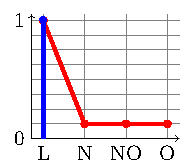
\includegraphics[width=\linewidth]{plot_tikz/speed1.pdf}
\caption{Initial}
\label{fig:a}
\end{subfigure}
\begin{subfigure}[t]{.15\linewidth}
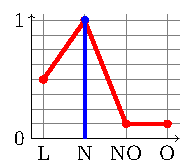
\includegraphics[width=\linewidth]{plot_tikz/speed12.pdf}
\caption{After 12 occurrences}
\label{fig:b}
\end{subfigure}
\begin{subfigure}[t]{.15\linewidth}
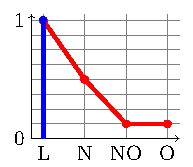
\includegraphics[width=\linewidth]{plot_tikz/speed17.pdf}
\caption{After 17 occurrences}
\label{fig:c}
\end{subfigure}
\begin{subfigure}[t]{.15\linewidth}
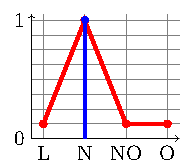
\includegraphics[width=\linewidth]{plot_tikz/speed22.pdf}
\caption{After 22 occurrences}
\label{fig:e}
\end{subfigure}
\begin{subfigure}[t]{.15\linewidth}
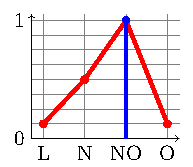
\includegraphics[width=\linewidth]{plot_tikz/speed24.pdf}
\caption{After 24 occurrences}
\label{fig:f}
\end{subfigure}
\begin{subfigure}[t]{.15\linewidth}
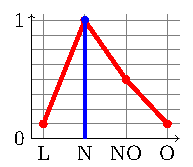
\includegraphics[width=\linewidth]{plot_tikz/speed27.pdf}
\caption{After 27 occurrences}
\label{fig:g}
\end{subfigure}
\\
\vspace{0.5cm}
\begin{subfigure}[b]{.15\linewidth}
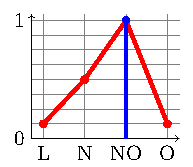
\includegraphics[width=\linewidth]{plot_tikz/speed28.pdf}
\caption{After 28 occurrences}
\label{fig:h}
\end{subfigure}
\begin{subfigure}[b]{.15\linewidth}
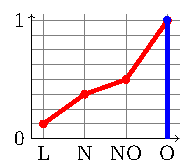
\includegraphics[width=\linewidth]{plot_tikz/speed29.pdf}
\caption{After 29 occurrences}
\label{fig:i}
\end{subfigure}
\begin{subfigure}[b]{.15\linewidth}
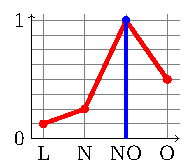
\includegraphics[width=\linewidth]{plot_tikz/speed30.pdf}
\caption{After 30 occurrences}
\label{fig:l}
\end{subfigure}
\begin{subfigure}[b]{.15\linewidth}
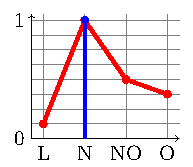
\includegraphics[width=\linewidth]{plot_tikz/speed31.pdf}
\caption{After 31 occurrences}
\label{fig:m}
\end{subfigure}
\begin{subfigure}[b]{.15\linewidth}
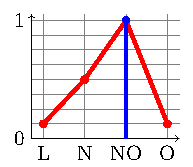
\includegraphics[width=\linewidth]{plot_tikz/speed33.pdf}
\caption{After 33 occurrences}
\label{fig:o}
\end{subfigure}
\begin{subfigure}[b]{.15\linewidth}
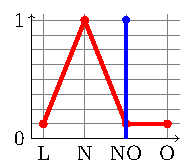
\includegraphics[width=\linewidth]{plot_tikz/speed28CONF.pdf}
\caption{After 34 occurrences}
\label{fig:speed34}
\end{subfigure}
\\
\vspace{0.5cm}
\caption[Possibilistic estimation on human assessment: experiment 1]{Experiment 1: Possibilistic estimation on human assessment of Airspeed (solid red curve), and actual machine state (blue bar). ``L'' is ``Low speed'', ``N'' is ``Normal speed'', ``NO'' is ``Near Overspeed'' and ``O'' is Overspeed.}
\label{fig:SpeedB}
\end{figure}

%\begin{figure}
%\centering
%\subfloat[\footnotesize  ]{\label{fig:a}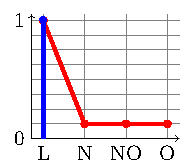
\includegraphics[width=0.41\linewidth]{plot_tikz/speed1.pdf}}  \hspace{0.3cm}
%\subfloat[\footnotesize ]{\label{fig:b}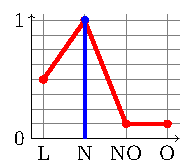
\includegraphics[width=0.41\linewidth]{plot_tikz/speed12.pdf}}\\
%\vspace{-0.15cm}
%\subfloat[\footnotesize After 17 occurrences ]{\label{fig:c}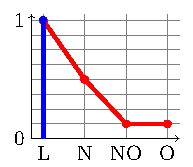
\includegraphics[width=0.41\linewidth]{plot_tikz/speed17.pdf}} \hspace{0.3cm}
%\subfloat[\footnotesize After 22 occurrences ]{\label{fig:e}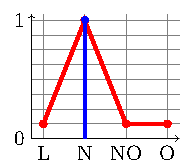
\includegraphics[width=0.41\linewidth]{plot_tikz/speed22.pdf}}\\
%\vspace{-0.15cm}
%\subfloat[\footnotesize After 24 occurrences]{\label{fig:f}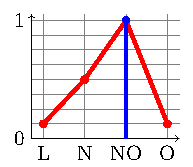
\includegraphics[width=0.41\linewidth]{plot_tikz/speed24.pdf}} \hspace{0.3cm}
%\subfloat[\footnotesize After 27 occurrences]{\label{fig:g}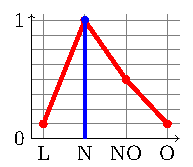
\includegraphics[width=0.41\linewidth]{plot_tikz/speed27.pdf}} \\
%\vspace{-0.15cm}
%\subfloat[\footnotesize After 28 occurrences]{\label{fig:h}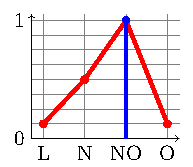
\includegraphics[width=0.41\linewidth]{plot_tikz/speed28.pdf}} \hspace{0.3cm}
%\subfloat[\footnotesize After 29 occurrences]{\label{fig:i}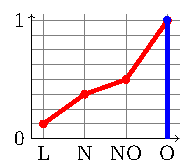
\includegraphics[width=0.41\linewidth]{plot_tikz/speed29.pdf}}\\
%\vspace{-0.15cm}
%\subfloat[\footnotesize After 30 occurrences]{\label{fig:l}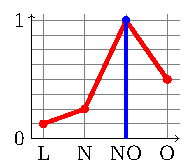
\includegraphics[width=0.41\linewidth]{plot_tikz/speed30.pdf}} \hspace{0.3cm}
%\subfloat[\footnotesize After 31 occurrences ]{\label{fig:m}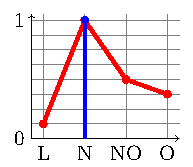
\includegraphics[width=0.41\linewidth]{plot_tikz/speed31.pdf}}\\
%\vspace{-0.15cm}
%\subfloat[\footnotesize After 33 occurrences]{\label{fig:o}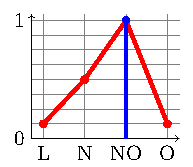
\includegraphics[width=0.41\linewidth]{plot_tikz/speed33.pdf}} \hspace{0.3cm}
%\subfloat[\footnotesize After 34 occurrences]{\label{fig:speed34}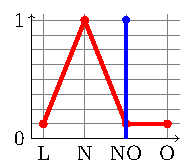
\includegraphics[width=0.41\linewidth]{plot_tikz/speed28CONF.pdf}}
%\caption{Experiment 1: Possibilistic estimation on human assessment of Airspeed (continuous red curve), and actual machine state (blue bar). ``L'' is ``Low speed'', ``N'' is ``Normal speed'', ``NO'' is ``Near Overspeed'' and ``O'' is Overspeed.}
%\label{fig:SpeedB}
%\end{figure}

The sequence of occurrences 
generated from the data 
recorded during the experience 
with the first participant 
is shown hereafter. 
A total of $57$ occurrences 
(among which are some selections) 
have been generated:

%\begin{framed}
\begin{footnotesize}
`Initialization', `Control Stick Off', `Throttle lever On', `Throttle lever Off', `Throttle lever On', `Throttle lever Off', `Throttle lever On', `Throttle lever Off', `Throttle lever On', `Throttle lever Off', `Control Stick On', `Speed Normal', `Control Stick Off', `Control Stick On', `ATHR button', `Control Stick Off', `SpeedLow', `Speed Normal', `Control Stick On', `Control Stick Off', `Control Stick On', `AP button', `Control Stick Off', `Near overspeed', `Control Stick On', `Control Stick Off', `Speed Normal', `Near overspeed', `Overspeed', `Near overspeed', `Speed Normal', `AP button', `Near overspeed', `Trajectory divergence',  `AP button', `Control Stick On',  `Control Stick Off', `Control Stick On', `Control Stick Off', `Control Stick On', `Control Stick Off', `Control Stick On', `Control Stick Off', `Control Stick On', `Control Stick Off', `Control Stick On', `Control Stick Off', `Control Stick On', `Control Stick Off', `AP button', `Trajectory divergence', `AP button', `Control Stick On', `Speed Normal', `Near overspeed', `Control Stick Off'
\end{footnotesize}
%\end{framed}


%\begin{framed}
%\begin{footnotesize}
%`Initialization', `Control Stick Off', `Throttle lever On', `Throttle lever Off', `Throttle lever On', `Throttle lever Off', `Throttle lever On', `Throttle lever Off', `Throttle lever On', `Throttle lever Off', `Control Stick On', `Speed Normal', `Control Stick Off', `Control Stick On', `ATHR button', `Control Stick Off', `SpeedLow', `Speed Normal', `Control Stick On', `Control Stick Off', `Control Stick On', `AP button', `Control Stick Off', `Near overspeed', `Control Stick On', `Control Stick Off', `Speed Normal', `Near overspeed', `Overspeed', `Near overspeed', `Speed Normal', `AP button', `Near overspeed', `Trajectory divergence',  `AP button', `Control Stick On',  `Control Stick Off', `Control Stick On', `Control Stick Off', `Control Stick On', `Control Stick Off', `Control Stick On', `Control Stick Off', `Control Stick On', `Control Stick Off', `Control Stick On', `Control Stick Off', `Control Stick On', `Control Stick Off', `AP button', `Trajectory divergence', `AP button', `Control Stick On', `Speed Normal', `Near overspeed', `Control Stick Off'
%\end{footnotesize}
%\end{framed}

The initial machine state is:
\begin{description}
\item $s_1=$ AP state: Off;
\item $s_2=$ ATHR state: On;
\item $s_3=$ Airspeed: Underspeed;
\item $s_4=$ Control stick: Actioning;
\item $s_5=$ Throttle lever:  Not actioning.
\end{description}
After the firing of the $25$th occurrence, 
$119.5$ seconds from the beginning of the experiment, 
the analysis model detects an exception:
\begin{description}
\item \texttt{Exception description: `Control stick On when AP on!'}.
\end{description}
After the firing of the $34$th occurrence, 
$772.6$ seconds from the beginning of the experiment, 
the analysis model detects an exception and explains it:
\begin{description}
\item \texttt{Exception description: `Vertical speed divergence $>$ 250 ft, unnoticed' because 'Speed becomes $>$Vmax-5, but unseen!'}.
\end{description}

After the firing of the $51$st occurrence, 
$886.1$ seconds from the beginning of the experiment, 
an exception is explained again:
\begin{description}
\item \texttt{Exception description: `Vertical speed divergence $>$ 250 ft, unnoticed' because 'Speed becomes $>$Vmax-5, but unseen!'}.
\end{description}
It is worth noting that the experimenters \cite{pizziol14} 
reported two human automation conflicts 
corresponding to the second and third exceptions, 
and that their findings on those conflicts causes 
(based on the observation of the data, 
the video recording and the interview of the pilot) 
is in agree with the exception explanation provided 
by the analysis model here.

After the execution of the $57$ occurrences, 
$196$ assessment trajectories are considered as possible 
(with different possibility degrees). 
The computation time is $30$ seconds. 
Some possibilistic estimations of the human assessment of the machine state 
variable ``Airspeed''
are represented in Figure \ref{fig:SpeedB}:
the possibility distribution over the human assessment $h$
of the airspeed, $\pi_t(h)$, is indicated by the red curve. 
This possibilistic evaluation is qualitative, 
nevertheless in the graphic representation, 
quantitative values are arbitrarily assigned 
to the possibility degrees 
(respecting qualitative ordering) to plot them. 
The actual machine state $s$ is stated 
by the blue bar with value $1$ on the y-axis:
if no exception arises, most possible assessment $h$ 
should be the actual state (blue bar). 
%Moreover 
%the second most possible estimate should be the former value (prior to the last fired occurrence) 
%of the actual state. The third most possible estimate should be the value of the actual state prior to the last two changes and so on.

%\begin{figure}
%\centering
%\subfloat[\footnotesize Initial ]{\label{fig:a}\includegraphics[width=0.5\linewidth]{Speed1.png}}  
%\subfloat[\footnotesize After 12 occurrences]{\label{fig:b}\includegraphics[width=0.5\linewidth]{Speed12.png}}\\

%\subfloat[\footnotesize After 17 occurrences ]{\label{fig:c}\includegraphics[width=0.5\linewidth]{Speed17.png}}  
%\subfloat[\footnotesize After 22 occurrences ]{\label{fig:e}\includegraphics[width=0.5\linewidth]{Speed22.png}}\\

%\subfloat[\footnotesize After 24 occurrences]{\label{fig:f}\includegraphics[width=0.5\linewidth]{Speed24.png}} 
%\subfloat[\footnotesize After 27 occurrences]{\label{fig:g}\includegraphics[width=0.5\linewidth]{Speed27.png}} \\

%\subfloat[\footnotesize After 28 occurrences]{\label{fig:h}\includegraphics[width=0.5\linewidth]{Speed28.png}}
%\subfloat[\footnotesize After 29 occurrences]{\label{fig:i}\includegraphics[width=0.5\linewidth]{Speed29.png}}\\

%\subfloat[\footnotesize After 30 occurrences]{\label{fig:l}\includegraphics[width=0.5\linewidth]{Speed30.png}}
%\subfloat[\footnotesize After 31 occurrences ]{\label{fig:m}\includegraphics[width=0.5\linewidth]{Speed31.png}}\\

%\subfloat[\footnotesize After 33 occurrences]{\label{fig:o}\includegraphics[width=0.5\linewidth]{Speed33.png}}
%\subfloat[\footnotesize After 34 occurrences]{\label{fig:speed34}\includegraphics[width=0.5\linewidth]{Speed28CONF.png}}
%\caption{Speed possibility distribution, {\color{blue} blue actual (s)}, {\color{red} red estimation (h)} }
%\label{fig:SpeedB}
%\end{figure}



Remember that after the firing of $34$ occurrences 
an exception is detected by the analysis model, 
which is graphically highlighted in Figure \ref{fig:speed34}: 
most possible human assessment is no more the real machine state.
% the objective assessment trajectory is no longer considered as normal\footnote{The possibility for a normal occurrence is 1.}. 
%Also after an exception the most possible estimation for the human assessment of the internal state (which is wrong in this case) is given by the maximum of the red line.

\subsubsection{Example 2}


\begin{figure}\centering
\begin{subfigure}[t]{.15\linewidth}
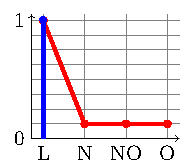
\includegraphics[width=\linewidth]{plot_tikz/speed1.pdf}
\caption{Initial}
\label{fig:a}
\end{subfigure}
\begin{subfigure}[t]{.15\linewidth}
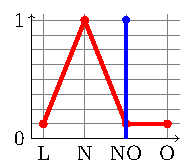
\includegraphics[width=\linewidth]{plot_tikz/speed28CONF.pdf}
\caption{After 18 occurrences}
\label{fig:b}
\end{subfigure}
\begin{subfigure}[t]{.15\linewidth}
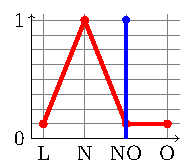
\includegraphics[width=\linewidth]{plot_tikz/speed28CONF.pdf}
\caption{After 46 occurrences}
\label{fig:c}
\end{subfigure}
\begin{subfigure}[t]{.15\linewidth}
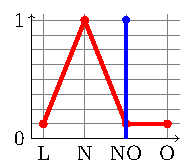
\includegraphics[width=\linewidth]{plot_tikz/speed28CONF.pdf}
\caption{After 49 occurrences}
\end{subfigure}
\\
\vspace{0.5cm}
\caption[Possibilistic estimation on human assessment: experiment 2]{Experiment 2: Possibilistic estimation on human assessment of speed (solid red curve), actual machine state (blue bar).}
\label{fig:SpeedC}
\end{figure}


A sequence of occurrences has been generated 
from the data recorded during experience 
with a second participant. 
A total of $85$ occurrences (among which are some human selections) have been generated. 
Hereafter the beginning of the sequence:

%\begin{framed}
\begin{footnotesize}
`Initialization', `Throttle lever On', `Throttle lever Off', `ATHR button', `Throttle lever On' ...
\end{footnotesize}
%\end{framed}

%
%:
%
%\begin{framed}
%\begin{footnotesize}
%`Initialization', 'Throttle lever On', `Throttle lever Off', `ATHR button', `Control Stick On', `Throttle lever On', `Throttle lever Off', `ATHR button', `ATHR button', `Control Stick Off', `Control Stick On', `ATHR button', `Control Stick Off', `Speed Normal', `Control Stick On', `Control Stick Off', `AP button', `Near overspeed', `Speed Normal', `Near overspeed', `Overspeed', `Near overspeed', `Overspeed', `Near overspeed', `Speed Normal', `Control Stick On', `Control Stick Off', `Control Stick On', `Control Stick Off', `Control Stick On', `Control Stick Off', `Control Stick On', `Near overspeed', `Speed Normal', `Near overspeed', `Speed Normal', `Near overspeed', `Speed Normal', `Near overspeed', `Overspeed', `Near overspeed', `Control Stick Off', `Speed Normal', `AP button', `Near overspeed', `ATHR button', `exceedingVzLevel1', `Throttle lever On', `Throttle lever Off', `Throttle lever On', `Throttle lever Off', `Throttle lever On', `Throttle lever Off', `Throttle lever On', `Throttle lever Off', `Control Stick On', `Speed Normal', `Control Stick Off', `Throttle lever On', `Throttle lever Off', `Throttle lever On', `Throttle lever Off', `Throttle lever On', `Throttle lever Off', `Throttle lever On', `Throttle lever Off', `Throttle lever On', `Throttle lever Off', `Throttle lever On', `Throttle lever Off', `Throttle lever On', `Throttle lever Off', `Throttle lever On', `Throttle lever Off', `Throttle lever On', `Throttle lever Off', `Throttle lever On', `Throttle lever Off', `Throttle lever On', `Throttle lever Off', `Throttle lever On', `Throttle lever Off', `Throttle lever On', `Throttle lever Off', `ATHR button'
%\end{footnotesize}
%\end{framed}

Initial machine state variables are the same as previously, 
except of control stick, which is here initially actioning.
%%\vspace{-0.7\baselineskip} 
%\begin{description}
%\item AP state: Off
%\item ATHR state: On
%\item  Airspeed: Underspeed
%\item Control stick:  Not actioning
%\item  Throttle lever:  Not actioning
%\end{description}
%%\vspace{-0.7\baselineskip} 

%\begin{figure}[t!]
%%\vspace{-\baselineskip} 
%\centering
%\subfloat[\footnotesize Initial ]{\label{fig:a}\includegraphics[width=0.5\linewidth]{Speed1.png}}  
%\subfloat[\footnotesize After 18 occurrences]{\label{fig:b}\includegraphics[width=0.5\linewidth]{Speed28CONF.png}}\\
%\vspace{-0.4cm}
%\subfloat[\footnotesize After 46 occurrences ]{\label{fig:c}\includegraphics[width=0.5\linewidth]{Speed28CONF.png}}  
%\subfloat[\footnotesize After 49 occurrences]{\label{fig:d}\includegraphics[width=0.5\linewidth]{Speed28CONF.png}}\\
%\caption{Speed possibility distribution, {\color{blue} blue actual (s)}, {\color{red} red estimation (h)} }
%\label{fig:SpeedC}
%\end{figure}




This second example was chosen because of the second occurrence, 
$30.2$ seconds from the beginning of the experiment.
The analysis model detects the following exception:
\begin{description}
\item \texttt{Exception description: `Throttle lever On when ATHR on!' because 'Wrong state initialization'}
\end{description}
Initially the ATHR is on: operating the throttle lever has no result 
(this action is considered as a slip). 
The model explains this slip as the result of a wrong initial assessment: 
if the pilot initial assessment of the ATHR state was Off, 
that could explain the execution of this action as nominal. 
It is worth noting that after giving up this useless action (`Throttle lever Off') 
the participant deactivated the ATHR (`ATHR button') 
and she/he started again operating the throttle lever ('Throttle lever On'), 
probably because she/he had a wrong initial situation assessment 
(as the found exception explanation) and she/he understood their assessment error. 

%\begin{figure}[t!]
%\centering
%\subfloat[\footnotesize Initial ]{\label{fig:a}\includegraphics[width=0.5\linewidth]{marpaATHRstate1.png}}  
%\subfloat[\footnotesize After 2 occurrences]{\label{fig:b}\includegraphics[width=0.5\linewidth]{marpaATHRstate2.png}}\\
%\caption{ATHR state possibility distribution.}
%\label{fig:ATHR}
%%\vspace{-\baselineskip} 
%\end{figure}
The analysis model detected also three times the same exception as for the previous participant:
\begin{description}
\item \texttt{Exception description: `Vertical speed divergence $>$ 250 ft, unnoticed' because 'Speed becomes $>$Vmax-5, but unseen!'}
\end{description}
Figure \ref{fig:SpeedC} shows the estimation of the human assessment 
of the speed, initially, and when these exceptions occur.

\section{Conclusion}
This chapter proposes a model for the human-machine interaction based 
on a machine model and expert knowledge on an human assessment error model.
The human-machine interaction is modelled as a possibilistic hidden Markov process. 
Qualitative Possibility Theory has been chosen because 
it is well suited to handle uncertainty defined by expert knowledge. 
The proposed possibilistic analysis model provides 
an estimation of the human assessment of the machine state 
and detects assessment errors. 
The analysis model is able to provide also an explanation (diagnosis) 
when an assessment error is detected.

This process of detection/identification 
could be used in real time applications in order to 
inform the human operator of their assessment errors.
It can help to make them correct their situation awareness 
and prevent the execution of other errors.

This work is based on the simplifying assumption 
that the human operator is certain about the state 
of the machine: a possible extension of this model 
may be to drop this assumption using a more refined 
representation of the human state assessment, 
as a set of machine states, or an uncertainty 
measure over the machine states.

This article proposes a model for the human-machine interaction based 
on a machine model and expert knowledge on an human assessment error model.
The human-machine interaction is modelled as a possibilistic hidden Markov process. 
Qualitative Possibility Theory has been chosen because 
it is well suited to handle uncertainty defined by expert knowledge. 
The proposed possibilistic analysis model provides 
an estimation of the human assessment of the machine state 
and detects assessment errors. 
The analysis model is able to provide also an explanation (diagnosis) 
when an assessment error is detected.

This process of detection/identification 
could be used in real time applications in order to 
inform the human operator of their assessment errors.
It can help to make them correct their situation awareness 
and prevent the execution of other errors.

This work is based on the simplifying assumption 
that the human operator is certain about the state 
of the machine: a possible extension of this model 
may be to drop this assumption using a more refined 
representation of the human state assessment, 
as a set of machine states, or an uncertainty 
measure over the machine states.



% ============================================================
% 
\chapter{Un Mod\`ele Hybride: Planifier dans des Domaines Partiellement Observable 
avec des \'Etats \'Epist\'emiques Flous et une Dynamique Probabiliste}
\label{chap_hybrid}
%%%%%%%%%%%%%%%%%%%%%%%%%%%%%%%%%%%%%%%%%%%%%%%%%%%%%%%%%%%%%%%%%%%%%%%
% TODO TODO TODO TODO TODO TODO TODO TODO TODO TODO TODO TODO TODO TODO
%%%%%%%%%%%%%%%%%%%%%%%%%%%%%%%%%%%%%%%%%%%%%%%%%%%%%%%%%%%%%%%%%%%%%%%
%\vide{
JOHN:
\textbf{Conclusion :}
\begin{itemize}
\item On a d�velopp� un mod�le hybride
\item On veut le tester sur un cas r�el de robotique mobile avec vision artificielle
\end{itemize}
ME:
%\subsection{Cr\'eation d'un mod\`ele POMDP hybride}
\textbf{OBJ:} cr\'eation d'un mod\`ele hybride, 
regroupant les qualit\'es des processus probabilistes et possibilistes:
discr\'etisation formelle des croyances, conservation des r\'ecompenses quantitatives, dynamique probabiliste (traduction en MDP classique) \\
POUR CELA:
\begin{itemize}
\item \'etude des solvers MDP de recherche dans l'espace d'\'etat (PROST, facto, d\'eterminism, RDDL, ...) \\
\textit{afin de r\'esumer les qualit\'ees requises par notre traduction}
\item mise en place d'une traduction d'un POMDP en POMDP hybride (MDP)
\begin{enumerate}
\item probabilit\'e pignistique 
\item int\'egrale de Choquet, 
\end{enumerate}
\item factorisation des croyances \`a hypoth\`eses simples 
\item on teste sur IPPC track PO \\
\textit{afin d'illustrer les performances de cet algorithme}
\end{itemize}

\subsection{POUR CHAP4 Consistance, Pr�servation de la pr�f�rence et Transformations} \label{transf} 
POUR CHAPITRE 4: transfos!\\

Cette vision donne une id�e [trouver r�f�rences] de simulation (probabiliste) d'�v�nements dont l'incertitude est mod�lis�e en terme de possibilit�s:
\begin{itemize}
\item[$\bullet$] Simuler $\alpha$ de loi uniforme sur $[0,1]$,
\item[$\bullet$] Tirer uniform�ment $\omega$ dans $\set{\omega \sachant \Pi(\omega) \geqslant \alpha}$
\end{itemize}
Ainsi, la probabilit� que l'�v�nement $\omega$ se produise est
\begin{eqnarray}
\nonumber \mathbf{p}(\omega) & = & \int_0^1 \mathbf{p} \paren{ \omega,\alpha} d \alpha \\
\nonumber & =  & \int_0^1 \mathbf{p} \paren{ \omega \sachant\alpha} d \alpha \\
\nonumber & = & \int_0^1 \dfrac{\mathds{1}_{\paren{ \Pi(\omega) \geqslant \alpha}}}{ \# \set{ \omega' \in \Omega \sachant \Pi(\omega')\geqslant \alpha }} d \alpha \\
\nonumber & = & \sum_{i=1}^n \int_{\alpha_{i+1}}^{\alpha_i} \dfrac{\mathds{1}_{\paren{ \Pi(\omega) \geqslant \alpha_i}}}{ \# \set{ \omega' \in \Omega \sachant \Pi(\omega')\geqslant \alpha_i }} d \alpha \\
\label{transf_simu} & = & \sum_{i=i_0 \vert \Pi(\omega)=\alpha_{i_0} }^n  \dfrac{\alpha_i-\alpha_{i+1}}{ \# A_i }
\end{eqnarray}
Nous retrouverons cette id�e avec la transformation r�versible $\Pi \leftrightarrow \mathbf{p}$ dans la section qui suit.


Il est essentiel de bien saisir que probabilit�s et possibilit�s ne mod�lisent pas la m�me facette de l'incertitude: une distribution de probabilit� pourra bien exprimer l'al�a, voire l'ind�cision (probabilit� uniforme), et la th�orie des possibilit�s est id�ale pour repr�senter l'ignorance. Cela nous am�ne � affirmer qu'une distribution de possibilit� contient moins d'information qu'une distribution de probabilit�. \\

Cependant, ces mesures restent des �valuations de l'incertitude, qui est un m�lange des diff�rentes facettes dont nous avons parl�es. Nous remarquons aussi qu'elles co�ncident lors de la connaissance totale (1 pour l'�v�nement certain, 0 pour les autres). Ces quelques �l�ments nous laissent penser que les deux mesures sont corr�l�es lorsqu'elles �valuent le m�me ph�nom�ne. Sous cet angle de vue, nous souhaitons d�finir des \textit{transformations} entre possibilit�s et probabilit�s qui prennent en compte ces dites corr�lations. \\
Des principes � respecter permettent aux transformations $\mathbf{p} \leftrightarrow \Pi$ de garder un sens.\\
Formellement, une mesure de possibilit�  $\Pi$ sur $\Omega$ est �quivalente � la famille de mesures de probabilit� $\mathcal{P}(\Pi)=\set{\mathbf{p} \in \Delta \Omega \sachant \forall A \subset \Omega, \ \mathbf{p}(A) \leqslant \Pi(A) }$ comme expliqu� dans \cite{DuPr1988.4}. Il para�t alors naturel de chercher des transformations respectant le principe de consistance.

\begin{Def}[Principe de consistance]
\label{consist}
\begin{equation*}
\forall A \subset \Omega,  \hspace{1cm} \Pi(A) \geqslant \mathbf{p}(A)
\end{equation*}
\end{Def}
Notons que
\begin{eqnarray*}
\Rightarrow \forall A \subset \Omega, & 1-\mathcal{N}(A^c) \geqslant 1-\mathbf{p}(A^c) \\
\Rightarrow \forall A \subset \Omega, & \mathcal{N}(A^c) \leqslant \mathbf{p}(A^c) \\
\end{eqnarray*}
et donc $\forall A \subset \Omega $, $\mathcal{N}(A) \leqslant \mathbf{p}(A)$. \\

Le principe suivant parait encore plus �vident: un �v�nement est plus probable qu'un autre si et seulement si il est plus possible qu'un autre. L'ordre de pr�f�rence induit par une distribution de possibilit� est en fait la signification principale de cette distribution.
\begin{Def}[Principe de la conservation de pr�f�rence] 
\label{conserv_pref}
\begin{equation*}
\forall \omega_1, \omega_2 \in \Omega^2,   \hspace{1cm}  \mathbf{p}(\omega_1) > \mathbf{p}(\omega_2) \Leftrightarrow \Pi(\omega_1) > \Pi(\omega_2)
\end{equation*}
\end{Def}
Ces deux principes nous guideront dans la construction de la transformation que nous recherchons. \\
\\
\textbf{Une transformation na�ve} peut facilement nous venir � l'esprit: \\
nous rappelons que la normalisation utilis�e en th�orie des possibilit�s est $\max_{\omega \in \Omega} \Pi(\omega) = 1$. Compte tenu des normalisations dans les deux th�ories, une transformation pourrait �tre: \\
\begin{eqnarray*}
\forall \omega \in \Omega, &  \Pi(\omega) = \dfrac{ \mathbf{p}(\omega) }{ \displaystyle \max_{\omega' \in \Omega} \mathbf{p}(\omega')}  \\
& \mathbf{p}(\omega) = \dfrac{\Pi(\omega)}{\displaystyle \sum_{\omega' \in \Omega}\Pi(\omega')}  
\end{eqnarray*}
Il est �vident que cette transformation respecte le principe de la conservation de pr�f�rence \ref{conserv_pref}. Cependant, le contre-exemple suivant nous assure que le principe de consistance \ref{consist} n'est pas respect� en g�n�ral: consid�rons 3 �v�nements, ($\# \Omega=3$) et la distribution de probabilit� $ \mathbf{p}(\omega_1)=0.9, \\  \mathbf{p}(\omega_2)= \mathbf{p}(\omega_3) =0.05$. \\
Cette probabilit� devient, par la transformation na�ve, la distribution de possibilit� $ \Pi(\omega_1)=1, \Pi(\omega_2)=\Pi(\omega_3)=\frac{1}{18} $. \\
Ainsi, \[ \Pi(\{ \omega_2 , \omega_3 \}) = \max(\Pi(\omega_2),\Pi(\omega_3)) = \frac{1}{18} < 0.1 = \mathbf{p}(\{ \omega_1,\omega_2  \})  \]
donc cette transformation ne respecte pas le principe de consistance.
\\

Reprenons le calcul de \ref{transf_simu} qui est une transformation $\Pi \rightarrow \mathbf{p}$. Cette \textbf{transformation r�versible} nous satisfera: elle est propos�e dans ~\cite{ DuPr1983.2} et respecte les principes de consistance  \ref{consist} et de conservation de la pr�f�rence \ref{conserv_pref}.\\
Supposons que $\Omega = \{ \omega_1,\ldots,\omega_m \}$ avec $\Pi(\omega_1) \geqslant \Pi(\omega_2) \geqslant \ldots \geqslant \Pi(\omega_m)$. Nous rappelons que $\alpha_1,\ldots,\alpha_n$ sont les diff�rentes valeurs pr�sentes dans la distribution de possibilit�, tri�es par ordre d�croissant. Nous rappelons aussi que $A_i=\set{\omega \in \Omega \sachant \Pi(\omega) \geqslant \alpha_i }$. Ainsi, pour $k \in \{1,\ldots,m\}$
\begin{eqnarray*}
\mathbf{p}(\omega_k) & = & \sum_{i=i_0 \vert \Pi(\omega_k)=\alpha_{i_0} }^n  \dfrac{\alpha_i-\alpha_{i+1}}{ \# A_i } \\
& = & \sum_{i=k}^m \dfrac{\Pi(\omega_i) - \Pi(\omega_{i+1})}{i}
\end{eqnarray*}
En effet, $\dfrac{\Pi(\omega_i) - \Pi(\omega_{i+1})}{i}$ est nul lorsque $\omega_i$ et $\omega_{i+1}$ ont la m�me possibilit�. Les seuls termes de la derni�re somme qui sont non nuls sont ceux tels que $\Pi(\omega_i)-\Pi(\omega_{i+1})>0$, soit ceux du type $\dfrac{\Pi(\omega_{\#(A_i)})-\Pi(\omega_{\#(A_i)+1})}{\#(A_i)}$ pour $i \in \{1,\ldots,n \}$,  car $\omega_{\#(A_i)} \in A_i$ et $\omega_{\#(A_i)+1} \notin A_i$.
\\

Explicitons la transformation propos�e:
Nous notons $\Omega= \set{\omega_1,\ldots,\omega_m}$, avec
$\mathbf{p}(\omega_1) \geqslant \mathbf{p}(\omega_2) \geqslant \ldots \geqslant \mathbf{p}(\omega_m)$. \\
Nous pouvons alors �crire la transformation $\mathbf{p} \rightarrow \Pi$ comme suit:
\begin{eqnarray}
\label{transf_rev1} & \forall i \in \{1,\ldots,m-1 \} &  \Pi(\omega_i) = i.\mathbf{p}(\omega_i) + \sum_{j=i+1}^m \mathbf{p}(\omega_j)   \\
\nonumber & & \mbox{ avec  } \Pi(\omega_m)=m.\mathbf{p}(\omega_m) 
\end{eqnarray}
De m�me si les $\omega \in \Omega$ sont tels que $\Pi(\omega_1) \geqslant \Pi(\omega_2) \geqslant \ldots \geqslant \Pi(\omega_m)$, la transformation r�ciproque $\Pi \rightarrow \mathbf{p}$, �quivalente � \ref{transf_simu}, est alors:
\begin{eqnarray}
\label{transf_rec} \forall i \in \set{1,\ldots,m} & \mathbf{p}(\omega_i) =\displaystyle \sum_{j=i}^m \dfrac{\Pi(\omega_j)-\Pi(\omega_{j+1})}{j} \\
\nonumber \mbox{ avec la notation } &  \Pi(\omega_{m+1}) =0
\end{eqnarray}
V�rifions que les deux formules sont �quivalentes, puis montrons que les principes expos�s pr�c�demment sont bien v�rifi�s.
\begin{proof}
Montrons que la premi�re formule implique la seconde. Tout d'abord, nous avons
 $\mathbf{p}(\omega_m) = \dfrac{\Pi(\omega_m)}{m} $ par la seconde ligne de \ref{transf_rev1}, et ainsi
\begin{eqnarray*}
 \Pi(\omega_{m-1}) & = & (m-1) \mathbf{p}(\omega_{m-1}) + \mathbf{p}(\omega_m)  \\
& \Downarrow & \\ 
\mathbf{p}(\omega_{m-1}) & = & \dfrac{\Pi(\omega_{m-1})}{m-1} - \dfrac{\Pi(\omega_m)}{m(m-1)} \\
 & = & \dfrac{\Pi(\omega_{m-1}) - \pi(\omega_m)}{m-1} + \dfrac{\Pi(\omega_m)}{m}
\end{eqnarray*}

Maintenant, supposons que pour $i_0 \in \set{2,\ldots,m-1}$ \ref{transf_rec} est vrai et montrons l'�galit� au rang $i_0-1$:
\begin{eqnarray}
\nonumber \Pi(\omega_{i_0-1}) - \Pi(\omega_{i_0}) & = & (i_0-1). \mathbf{p}(\omega_{i_0-1}) + \sum_{j=i_{0}-1}^{m} \mathbf{p}(\omega_{j}) - i_0.\mathbf{p}(\omega_{i_0}) - \sum_{j=i_0}^m \mathbf{p}(\omega_j) \\
\nonumber & = & (i_0-1). \mathbf{p}(\omega_{i_0-1}) - i_0.\mathbf{p}(\omega_{i_0}) + \mathbf{p}(\omega_{i_0-1}) \\
\nonumber & = & (i_0-1)(\mathbf{p}(\omega_{i_0-1})-\mathbf{p}(\omega_{i_0})) \\
\label{cons_pref_poss_prob}  \Rightarrow  \mathbf{p}(\omega_{i_0-1}) & = & \mathbf{p}(\omega_{i_0}) + \dfrac{\Pi(\omega_{i_0-1}) - \Pi(\omega_{i_0})}{i_0 -1} \\
\nonumber & = & \displaystyle \sum_{j=i_0-1}^m \dfrac{\Pi(\omega_j)-\Pi(\omega_{j+1})}{j} 
\end{eqnarray}
Montrons maintenant l'implication r�ciproque: la seconde formule pour $i=m$ nous donne directement la seconde ligne de \ref{transf_rev1}. Puis,
\begin{eqnarray*}
\mathbf{p}(\omega_{m-1}) & = & \sum_{j=m-1}^m \dfrac{\Pi(\omega_j) - \Pi(\omega_{j-1})}{j} \\
& = & \dfrac{\Pi(\omega_{m-1}) - \Pi(\omega_{m})}{m-1} + \mathbf{p}(\omega_m) \\
& & \Downarrow  \\
\Pi(\omega_{m-1}) & = & \Pi(\omega_m) + (m-1) (\mathbf{p}(\omega_{m-1}) -\mathbf{p}(\omega_m)) \\
& = & m\mathbf{p}(\omega_m) + (m-1) (\mathbf{p}(\omega_{m-1}) -\mathbf{p}(\omega_m)) \\
& = & (m-1) \mathbf{p}(\omega_{m-1}) - \mathbf{p}(\omega_m)
\end{eqnarray*}
Maintenant, supposons que la premi�re formule (\ref{transf_rev1}) est vraie pour $i_0 \in \{ 2 , \ldots, m-1  \}$, et montrons qu'elle est vraie au rang $i_0-1$.
\begin{eqnarray*}
\mathbf{p}(\omega_{i_0-1}) - \mathbf{p}(\omega_{i_0}) & = & \dfrac{\Pi(\omega_{i_0-1}) - \Pi(\omega_{i_0})}{i_0-1} \\
\Rightarrow \Pi(\omega_{i_0-1}) & = & \Pi(\omega_{i_0}) +  (i_0-1)(\mathbf{p}(\omega_{i_0-1}) - \mathbf{p}(\omega_{i_0})) \\
& = &  i_0.\mathbf{p}(\omega_{i_0}) + \sum_{j=i_0+1}^m \mathbf{p}(\omega_j) +  (i_0-1)(\mathbf{p}(\omega_{i_0-1}) - \mathbf{p}(\omega_{i_0})) \\
& = & \sum_{j=i_0}^m \mathbf{p}(\omega_j) +  (i_0-1)\mathbf{p}(\omega_{i_0-1})
\end{eqnarray*}
Les deux formules sont donc �quivalentes.\\

Montrons que le principe de consistance \ref{consist} est respect�: \\
Soit $A \in \Omega$, et $j_0 = \min \set{ j \sachant \omega_j \in A  }$. \\
\begin{eqnarray*}
\Pi(A)  = & \max_{\omega \in A}(\Pi(\omega)) & \\
= &  j_0. \mathbf{p}(\omega_{j_0}) + \displaystyle  \sum_{j=j_{0} +1}^m \mathbf{p}(\omega_j) & \geqslant  \sum_{j=j_0}^m \mathbf{p}(\omega_j) \\ 
 &  & \geqslant  \sum_{\omega \in A} \mathbf{p}(\omega) = \mathbf{p}(A)  
\end{eqnarray*}
par d�finition de $j_0$. La consistance est donc assur�e. \\

Le principe de conservation de la pr�f�rence \ref{conserv_pref} se voit bien avec la deuxi�me formule: \\
\begin{eqnarray*}
\mathbf{p}(x_i) - \mathbf{p}(x_{i+1}) & = & \displaystyle \sum_{k=i}^{i} \dfrac{\Pi(\omega_j)-\Pi(\omega_{j+1})}{j} \\
& = & \displaystyle \dfrac{\Pi(\omega_j)-\Pi(\omega_{j+1})}{j} 
\end{eqnarray*}
$\mathbf{p}(x_i) - \mathbf{p}(x_{i+1})>0 \Leftrightarrow \Pi(\omega_j)-\Pi(\omega_{j+1})>0$.
\end{proof}
Bien d'autres transformations existent \cite{1993.1}, cependant, pour les travaux que nous allons pr�senter, cette transformation r�versible est suffisante.
}
%%%%%%%%%%%%%%%%%%%%%%%%%%%%%%%%%
%%%%%%%%%%%%%%%%%%%%%%%%%%%%%%%%%
%%%%%%%%%%%%%%%%%%%%%%%%%%%%%%%%%
%%%%%%%%%%%%%%%%%%%%%%%%%%%%%%%%%
%%%%%%%%%%%%%%%%%%%%%%%%%%%%%%%%%
%%%%%%%%%%%%%%%%%%%%%%%%%%%%%%%%%
%%%%%%%%%%%%%%%%%%%%%%%%%%%%%%%%%

While the previous chapters dealt with purely qualitative possibilistic models,
this one proposes to use the strength of both probabilistic and possibilistic approaches,
in order to solve fully defined factored POMDPs, or partially defined ones.
This idea comes from the analysis of the results of the experiments of Chapter \ref{chap_symb}:
qualitative modeling may lead to poor strategies 
for risky problems, or when the frequentist information defining the POMDP 
is at the heart of planning the problem. 
Here, a new translation from Partially Observable MDP into Fully 
Observable MDP is described. 
Unlike the classical
translation (see Section \ref{section_POMDPisbeliefMDP}), 
the resulting problem state space is finite, 
making MDP solvers able to solve this simplified version 
of the initial partially observable problem: this approach encodes 
agent beliefs with fuzzy measures over states, 
leading to an MDP whose system state space is a finite set of 
epistemic states. %After a short description of the POMDP
%problem as well as notions of Possibility Theory,
The translation is described in a formal manner with
semantic arguments. Then actual computations of this transformation
are detailed, in order to highly benefits from the factorized 
structure of the initial POMDP in the the final MDP problem 
size reduction and structure.
Finally size reduction and tractability of the resulting MDP is 
illustrated on a simple POMDP problem.

%
% Introduction
% + SUM15

\section{Introduction}
%Partially Observable Markov Decision Processes (POMDPs) \cite{Smallwood_Sondik} can
%finely model an agent acting under uncertainty in a partially hidden environment.
%However, solving a POMDP, \textit{i.e.} computing an optimal strategy for the agent, is a
%really difficult task: the problem of deciding if there exists a strategy 
%leading to an expected reward greater than a given threshold
%for a finite horizon POMDP, is a
%%PSPACE-complete problem \cite{Papadimitriou:1987:CMD:35577.35581}. 
%Classical approaches try to solve this problem
%using Dynamic Programming \cite{Cassandra97incrementalpruning:}, or
%via approximate computation: for instance via point-based methods 
%\cite{Pineau_2003_4826}, \cite{Kurniawati-RSS08}, 
%heuristics \cite{Smith:2004:HSV:1036843.1036906}, or 
%Monte Carlo approach \cite{NIPS2010_4031}.

The approach proposed here simplifies the belief space of a POMDP problem before solving it.
The transformation described leads to a fully observable MDP on a finite
number of epistemic states, \textit{i.e.} a problem 
modeling an agent acting under uncertainty in a fully
observable environment \cite{puterman94}. As such a finite state space 
MDP problem is P-complete \cite{Papadimitriou:1987} 
this transformation qualifies as a simplification, and any MDP solver 
can return a policy for this translated POMDP.


%Most of the POMDP algorithms reason about the \textit{agent belief} during
%the process, defined as the probability of the actual system state knowing
%all the system observations and agent actions from the beginning.
%This belief is updated at each time step using the Bayes
%rule and the new observation. The initial belief, or \textit{a priori}
%probability distribution over the system states, takes part in
%the definition of the POMDP problem. However in practice, the initial system
%state can be unknown with absolutely no probabilistic information: 
%for instance, in a robotic exploration context, 
%the initial location of the agent, or the presence of an entity in the scene. 
%Defining the process with a uniform probability distribution as initial belief
%(\textit{e.g.} over all locations or over entity presence) is a subjectivist
%answer \cite{de1974theory}, \textit{i.e.} all probabilities are the same
%because no event is more plausible than another:
%it corresponds to equal betting rates. However following belief
%updates will eventually mix frequentist probability distributions 
%defining the POMDP problem with this initial belief which is a subjective probability, 
%and it does not always make sense. 

More than only a simplification of the initial POMDP problem,
the theoretical framework used here for belief states representation
formally models an agent's knowledge about the system state.
Indeed the proposed translation defines the belief states as possibility distributions
over system states $s \in \mathcal{S}$
% these kinds of distributions are denoted by $\pi$
%(the counterpart of probability notation $\textbf{p}$) and 
which represents the fuzzy set of possible system states, 
as done with $\pi$-POMDP models.



%the indicator (chararacteristic) function of this set.
%Unlike classical sets, values of a fuzzy set indicator function $\pi$
%are not only in $\set{0,1}$. Recall that the indicator function of
%a classical set $A \subseteq \mathcal{S}$ is $\mathds{1}_{A}(s) = 1$ 
%if $s \in A$ and $0$ otherwise.
%Values of a fuzzy set indicator function are chosen in a totally ordered scale 
%$\mathcal{L} = \set{ 1=l_1, l_2, \ldots, 0}$ with $l_1>l_2>\ldots>0$: 
%%$\pi: \mathcal{S} \rightarrow \mathcal{L}$. If $s \in \mathcal{S}$ is such that
%$\pi(s)=l_i$, $s$ is in the fuzzy set described by $\pi$, with degree $l_i$.  
%Possibilistic beliefs used in this work will represent fuzzy sets of possible 
%states. If the current possibilistic belief coincide with the distribution
%$\pi(s)=1$ $\forall s \in \mathcal{S}$, all system states are totally possible,
%and it models therefore a total ignorance about the current system state:
%qualitative possibilistic beliefs can model agent initial ignorance.
%The full knowledge of the current state, say $\tilde{s} \in \mathcal{S}$, 
%is encoded by a possibility distribution equal to the classical indicator
%function of the singleton $\pi(s) = \mathds{1}_{\set{ s=\tilde{s} }}(s)$.
%Between these two extrema, current knowledge of the system is described by
%a set of entirely possible states, $\set{ s \in \mathcal{S} \mbox{ s.t. } \pi(s)=1  }$,
%and successive sets of less plausible ones $\set{ s \in \mathcal{S} \mbox{ s.t. } \pi(s)=l_i}$
%down to the set of impossible states $\set{ s \in \mathcal{S} \mbox{ s.t. } \pi(s)=0  }$.

The major originality of this work comes from the finiteness of the scale $\mathcal{L}$:
indeed it follows that the number of possible belief states over the system state 
is, as well, finite (smaller than $\# ( \mathcal{L}^{\mathcal{S}} ) = 
(\# \mathcal{L})^{\# \mathcal{S}}$, see Equation \ref{equation_numberOfPossDistrib}). 
What very clearly distinguishes this approach
from the classical one is that the classical translation leads to an infinite set of 
belief states (the continuous set of all probability distributions over $\mathcal{S}$, 
or the sequence of reachable belief states from an initial one, see Section \ref{section_POMDPisbeliefMDP}).
The translation described here leads to an MDP whose system state space
is the set of possible possibilistic belief states, or \textit{epistemic states},
that is why its state space is finite. 

In addition to POMDP simplification and knowledge modelling, this qualitative
possibilistic framework offers some interesting properties: the possibilistic counterpart 
of the Bayes rule leads to a special belief state behaviour. Indeed the 
agent can possibly change their mind radically and rapidly, 
as described in Section \ref{EXPE_CHAP1}, 
experimental section of Chapter \ref{chap_Updates}.% \cite{Drougard13}. 
Moreover, under some conditions, the increased specificity of the belief state distribution is enforced, \textit{i.e.} 
the knowledge about the current state is non decreasing with time steps (see Section \ref{EXPE_CHAP1}).
Finally, in order to fully define the resulting MDP, the translation has to attach 
a reward function to its states: as a possibilistic belief state distributions 
constitute the new (epistemic) states of the problem, the definition of the rewards
uses the Choquet integral adapted to fuzzy measures. 
This integral is used with the dual measure of the possibility measure defined by the belief state. 
The dual measure of a possibility measure, called the \textit{necessity measure} (see Definition \ref{DEF_necessity}), 
and the use of this integral makes the rewards values pessimistic about the potential lack of knowledge
described by the associated belief state.

However the number of possibilistic belief distributions, or \textit{fuzzy epistemic states},
grows exponentially with the number of initial POMDP system states. 
The so called simplification of the problem does not transform the PSPACE POMDP 
problem into a polynomial one: as the new state space size is exponential in the 
previous one, the resulting problem is EXPTIME. The proposed translation 
tries to generate as few epistemic states as possible taking carefully into account
potential factorized structures of the initial POMDP.

%The first section is devoted to the presentation of Markov Decision Processes,
%the main concern of this paper. Tools from Possibility Theory are also
%defined to make this paper self-contained. 
This chapter begins with the description of 
the first contribution of this work, which is the translation itself, 
presented in a formal way.
As the resulting state space of the built MDP is too big to make this problem
tractable without factorization tricks in practice,
the next section details the proper way to preprocess its attributes.
Finally, the last section illustrates the power of this approach,
describing the translation in practice, 
and applying it on a simple factored POMDP problem.

%\section{Background}


%Partially Observable Markov Decision Processes (POMDPs) \cite{Smallwood_Sondik} can
%finely model an agent acting under uncertainty in a partially hidden environment.
%However, solving a POMDP, \textit{i.e.} computing an optimal strategy for the agent, is a
%really difficult task: the problem of deciding if there exists a strategy 
%leading to an expected reward greater than a given threshold
%for a finite horizon POMDP, is a
%%PSPACE-complete problem \cite{Papadimitriou:1987:CMD:35577.35581}. 
%Classical approaches try to solve this problem
%using Dynamic Programming \cite{Cassandra97incrementalpruning:}, or
%via approximate computation: for instance via point-based methods 
%\cite{Pineau_2003_4826}, \cite{Kurniawati-RSS08}, 
%heuristics \cite{Smith:2004:HSV:1036843.1036906}, or 
%Monte Carlo approach \cite{NIPS2010_4031}.
%Most of the POMDP algorithms reason about the \textit{agent belief} during
%the process, defined as the probability of the actual system state knowing
%all the system observations and agent actions from the beginning.
%This belief is updated at each time step using the Bayes
%rule and the new observation. The initial belief, or \textit{a priori}
%probability distribution over the system states, takes part in
%the definition of the POMDP problem. However in practice, the initial system
%state can be unknown with absolutely no probabilistic information: 
%for instance, in a robotic exploration context, 
%the initial location of the agent, or the presence of an entity in the scene. 
%Defining the process with a uniform probability distribution as initial belief
%(\textit{e.g.} over all locations or over entity presence) is a subjectivist
%answer \cite{de1974theory}, \textit{i.e.} all probabilities are the same
%because no event is more plausible than another:
%it corresponds to equal betting rates. However following belief
%updates will eventually mix frequentist probability distributions 
%defining the POMDP problem with this initial belief which is a subjective probability, 
%and it does not always make sense. 
%the indicator (chararacteristic) function of this set.
%Unlike classical sets, values of a fuzzy set indicator function $\pi$
%are not only in $\set{0,1}$. Recall that the indicator function of
%a classical set $A \subseteq \mathcal{S}$ is $\mathds{1}_{A}(s) = 1$ 
%if $s \in A$ and $0$ otherwise.
%Values of a fuzzy set indicator function are chosen in a totally ordered scale 
%$\mathcal{L} = \set{ 1=l_1, l_2, \ldots, 0}$ with $l_1>l_2>\ldots>0$: 
%%$\pi: \mathcal{S} \rightarrow \mathcal{L}$. If $s \in \mathcal{S}$ is such that
%$\pi(s)=l_i$, $s$ is in the fuzzy set described by $\pi$, with degree $l_i$.  
%Possibilistic beliefs used in this work will represent fuzzy sets of possible 
%states. If the current possibilistic belief coincide with the distribution
%$\pi(s)=1$ $\forall s \in \mathcal{S}$, all system states are totally possible,
%and it models therefore a total ignorance about the current system state:
%qualitative possibilistic beliefs can model agent initial ignorance.
%The full knowledge of the current state, say $\tilde{s} \in \mathcal{S}$, 
%is encoded by a possibility distribution equal to the classical indicator
%function of the singleton $\pi(s) = \mathds{1}_{\set{ s=\tilde{s} }}(s)$.
%Between these two extrema, current knowledge of the system is described by
%a set of entirely possible states, $\set{ s \in \mathcal{S} \mbox{ s.t. } \pi(s)=1  }$,
%and successive sets of less plausible ones $\set{ s \in \mathcal{S} \mbox{ s.t. } \pi(s)=l_i}$
%down to the set of impossible states $\set{ s \in \mathcal{S} \mbox{ s.t. } \pi(s)=0  }$.
%The work developed in this paper remains in the classical MDP and POMDP frameworks, 
%which are recalled in this section: 
%possibilistic material necessary to build the promised translation are then presented. 
%\subsection{Markov Decision Processes}
%A Markov Decision Process (MDP) \cite{Bel} is a well suited framework 
%for sequential decision making under uncertainty, 
%when the agent involved has full knowledge of the actual system state.
%Such a process is formally defined by a $4$-tuple 
%$\langle \mathcal{S}, \mathcal{A}, T, r \rangle$ where $\mathcal{S}$ is a finite
%set of system states $s \in \mathcal{S}$. The finite set $\mathcal{A}$ consists
%of all actions $a \in \mathcal{A}$ available for the agent. The Markov dynamics of the system
%are described by the transition function $T: \mathcal{S} \times \mathcal{A} \times \mathcal{S} \rightarrow [0,1]$. 
%This function is defined as the transition probability distribution
%of the system states for each action: if action $a \in \mathcal{A}$ is chosen by
%the agent, and the current system state is $s \in \mathcal{S}$, the next state $s' \in \mathcal{S}$
%is reached with probability $T(s,a,s') = \textbf{p} \paren{ s' \sachant s,a }$. Finally,
%a reward function $r: \mathcal{S} \times \mathcal{A} \rightarrow \mathbb{R}$ is defined
%to model the goal of the agent. Indeed, solving an infinite horizon MDP problem 
%consists in computing a \textit{strategy}, \textit{i.e.} a function $d$ 
%defined on $\mathcal{S}$ and whose values are actions $a \in \mathcal{A}$, 
%maximizing the expected discounted total reward: 
%\begin{equation}
%\label{criterion}
%\mathbb{E} \croch{ \sum_{t=0}^{+ \infty} \gamma^t r(s_t,d_t) },
%\end{equation}
%where $d_t=d(s_t)$ and $0<\gamma<1$ is the discount factor.

%A Partially Observable MDP (POMDP) \cite{Smallwood_Sondik} makes a step further
%in the modeling flexibility, allowing the agent not to know which system state
%is the current one. The formal definition of a POMDP is the $7$-tuple 
%$\langle \mathcal{S}, \mathcal{A}, T, \Omega, O, r, b_0 \rangle$, where the system state 
%$\mathcal{S}$, the set of actions $\mathcal{A}$, the transition function $T$ and the
%reward function $r$ remain the same as for the MDP definition. In this model, 
%the current system state $s \in \mathcal{S}$ cannot be used as available 
%information for the agent: the agent knowledge about the actual system state 
%comes from observations $o \in \Omega$, where $\Omega$ is a finite set. 
%The observation function $O: \mathcal{S} \times \mathcal{A} \times \Omega \rightarrow [0,1]$
%gives for each action $a \in \mathcal{A}$ and reached system state $s' \in \mathcal{S}$, 
%the probability over possible observations $o' \in \Omega$: $O(s',a,o') = \textbf{p} \paren{ o' \sachant s', a }$. Finally, the initial belief $b_0: \mathcal{S} \rightarrow [0,1]$ is the
%\textit{prior} probability distribution over the system state space $\mathcal{S}$: 
%$b_0(s) = \textbf{p} \paren{ s_0 = s }$, $\forall s \in \mathcal{S}$.

%At a given time step $t>0$, the agent belief is defined 
%as the probability of the $t^{th}$ state $s_t$
%conditionned on all the past actions and observations, 
%and with the prior $b_0$, \textit{i.e.}
%$b_t(s) = \textbf{p}_{s_0 \sim b_0} \paren{s_t = s \sachant a_0,o_1,\ldots,a_{t-1},o_t }$.
%It can be easily recursively computed using Bayes rule: at time step $t$, 
%if the belief is $b_t$, chosen action $a \in \mathcal{A}$ and new observation 
%$\tilde{o} \in \Omega$, next belief is
%\begin{eqnarray}
%\label{probBayesRule}
%b_{t+1}(s') = u(b_t,a,\tilde{o}) = \frac{ O(s',a,\tilde{o}) \cdot \sum_{s} T(s,a,s') b_t(s) }{ \sum_{\underline{s}, \overline{s}} O(\overline{s},a,\tilde{o}) \cdot T(\underline{s},a,\overline{s}) b_t(\underline{s})  } .
%\end{eqnarray}
%as illustrated by the Bayesian Network in Figure \ref{BayesNetPOMDP}.
%\begin{figure}\centering
%\begin{tikzpicture}
%%%%%%%%%%%%%%%%%%%%%%%%%%%%%%%%%%%%%%%%%%%%%%%%%%%%%%%%%%%%%%%
%vertex
%\tikzstyle{vertex}=[circle,fill=black!30,minimum size=20pt,inner sep=0pt]
%nodes
%\node[vertex] (state1) at (2,1.8) {$s_t$};
%\node[vertex] (state2) at (6,1.8) {$s_{t+1}$};
%\node[vertex] (obs) at (10,1) {$o_{t+1}$};
%\node[vertex] (action) at (2.5,0.5) {$a_t$};
%%bels
%\node (bel1) at (2.7,2.1) {$b_t(s)$};
%\node (bel2) at (7,2) {$b_{t+1}(s')$};
%%probas
%\node (trans) at (3.9,1.6) {$\textbf{p} \paren{ s_{t+1} \sachant s_t, a_t }$};
%\node (observ) at (7,1.1) {$\textbf{p} \paren{ o_{t+1} \sachant s_{t+1}, a_t }$};
%%%%%%%%%%%%%%%%%%%%%%%%%%%%%%%%%%%%%%%%%%%%%%%%%%%%%%%%%%%%%%%
%%ARROWS
%%\draw[->,>=latex, thick] (state1) -- (state2);
%\draw[->,>=latex, thick] (state2) -- (obs);
%\draw[->,>=latex, thick] (action) -- (state2);
%\draw[->,>=latex, thick] (action) -- (obs);
%\end{tikzpicture}
%\caption{Bayesian Network illustrating the belief update.}
%\label{BayesNetPOMDP}
%\end{figure}%

%As successive beliefs are computed 
%with the observations perceived by the agent,
%they are visible. Moreover, it can be easily shown that
%the expected total reward can be rewritten 
%\begin{equation}
%\label{probCriterion}
%\mathbb{E} \croch{ \sum_{t=0}^{+ \infty} \gamma^t r(s_t,d_t) } = \mathbb{E} \croch{ \sum_{t=0}^{+ \infty} \gamma^t r(b_t,d_t) }, 
%\end{equation}
%defining $r(b_t,a) = \sum_s r(s,a) \cdot b_t(s)$ as the reward of belief $b_t$.

%Let us denote by $\mathbb{P}_{\mathcal{S}}$ the infinite set of probability distributions 
%over $\mathcal{S}$: 
%solving the infinite horizon POMDP problem, consists in computing 
%a decision function $d: \mathbb{P}_{\mathcal{S}} \rightarrow \mathcal{A}$ such that
%$d_t = d(b_t)$ maximizes the criterion \ref{criterion}.
%seen as an MDP whose states are probabilistic beliefs,  
%an optimal strategy for the infinite horizon POMDP 
%is looked for among strategies 
%$d: \mathbb{P}_{\mathcal{S}} \rightarrow \mathcal{A}$ 
%such that successive $d_t = d(b_t)$ maximize 
%the expected total reward \ref{probCriterion}.

%As the focused problem (POMDP) has been formally defined, possibilistic tools
%are now presented in the next section.
%\subsection{Possibility Theory}
%In our context, distributions defined in the Possibility Theory framework  
%are valued in a totally ordered scale $\mathcal{L}=\set{ 1=l_1,l_2,\ldots,0 }$ with
%$l_1>l_2>\ldots>0$. A possibility measure $\Pi$ defined on $\mathcal{S}$ is a 
%fuzzy measure valued in $\mathcal{L}$, such that $\forall A,B \subset \mathcal{S}$, 
%$\Pi(A \cup B) = \max \set{ \Pi(A), \Pi(B) }$, $\Pi(\emptyset)=0$ and $\Pi(\mathcal{S})=1$.
%It follows that this measure is entirely defined by the associated possibility distribution,
%\textit{i.e.} the measure of the singletons: 
%$\forall s \in \mathcal{S}$, $\pi(s) = \Pi(\set{s})$. Properties of this measure lead to
%the possibilistic normalization: 
%\begin{equation} 
%\label{possNormDef}
%\max_{s \in \mathcal{S}} \pi(s) = \Pi(\mathcal{S}) = 1.
%\end{equation}
%If $\overline{s},\underline{s} \in \mathcal{S}$ 
%are such that $\pi(\overline{s})<\pi(\underline{s})$, it means
%that $\overline{s}$ is less plausible than $\underline{s}$. States with possibility
%degree $0$, \textit{i.e.} states $s \in \mathcal{S}$ such that $\pi(s)=0$, are impossible
%(same meaning as $\textbf{p}(s)=0$), and those such that $\pi(s)=1$ are entirely possible
%(but not necessary the most probable one).

%After the introduction of a possibility measure over a set $\Omega$, 
%the joint possibility measure on $\mathcal{S} \times \Omega$ 
%is defined in a qualitative way: 
%$\forall A \subset \mathcal{S}$, $\forall B \subset \Omega$
%\begin{eqnarray}
%\label{possInter} \Pi(A, B) = \min \set{ \Pi \paren{A \sachant B}, \Pi \paren{B}} = \min \set{ \Pi \paren{B \sachant A}, \Pi \paren{A}}.
%\end{eqnarray}
%ote the similarities between Possibility and Probability Theory, 
%replacing $\max$ by $+$ and $\min$ by $\times$. Moreover, Possibility Theory has its
%own counterpart of the Bayes rule \cite{Dubois199023}: 
%\begin{eqnarray}
%\label{possBayesRule} \Pi \paren{A \sachant B} = \left \{ \begin{array}{ccc} 1 \mbox{ if } \Pi(A, B)  =  \Pi(B) \\
% \Pi \paren{A, B} \mbox{ otherwise} \end{array} \right.
%\end{eqnarray}
%which is nothing more than the least specific measure satifying Equation \ref{possInter}.
%It can also be seen more easily as the joint measure normalized in a possibilistic
%manner, as in Equation \ref{possNormDef}.

%These few tools from Qualitative Possibility Theory are enough to define the announced
%translation. Next section is then devoted to building an MDP with fuzzy epistemic states
%from a POMDP.
\section{A Hybrid POMDP}
As claimed by Zadeh, ``most information/intelligent
systems will be of hybrid type'' \cite{DBLP:journals/soco/Zadeh98}:
the idea developped here is to use a granulated representation of the agent knowledge 
using possibilistic belief states instead of probabilistic belief states
in the POMDP framework.
The first advantage of this granulation
is that strategy computation
is performed reasoning on
a finite set of possibilistic belief states 
called then epistemic states:
the set of all possibility distributions 
defined over $\mathcal{S}$, denoted by $\Pi^{\mathcal{S}}_{\mathcal{L}}$ is
$\# \Pi^{\mathcal{S}}_{\mathcal{L}} = \# \mathcal{L}^{\# \mathcal{S}} - (\# \mathcal{L}-1)^{\# \mathcal{S}}$,
due to the possibilistic normalization (see Equation \ref{equation_numberOfPossDistrib}),
while the set of probability distributions over $\mathcal{S}$ is infinite.
%Possibilistic counterparts of POMDP, named $\pi$-(PO)MDPs have been already defined 
%\cite{Sabbadin_1999_pipomdp, LIP61498} and efficiently used for planning under uncertainty problems \cite{DBLP:conf/aaai/DrougardTFD14}. 
The $\pi$-MDPs studied in the first chapters of this thesis 
are quite different from the model exposed in this chapter. 
For instance, Qualitative Possibilistic MDPs 
do not use quantitative data as probabilities or rewards. 
Dynamics is described in a purely qualitative possibilistic way. 
Frequentist information about the problem cannot be encoded: 
these frameworks are indeed dedicated to situations 
when the probabilistic dynamic of the studied system is lacking.
Moreover, possible values of the reward function are chosen 
among the degrees of the qualitative possibilistic scale.
A commensurability assumption between reward and possibility 
degrees, i.e. a meaning of why they share the same scale, 
is needed to use the criteria proposed in these frameworks.
Our model bypasses these demands: a real number is assigned 
to each possibilistic belief (epistemic state), 
instead of a qualitative utility degree: 
it represents the reward got by the agent 
when reaching this belief (in a MDP fashion)
as detailed in Section \ref{aggreg}. 
Moreover, the dynamics of our process 
is described with probability distributions: 
approximate probabilistic transition functions 
between current and next beliefs, or epistemic states, 
are given section \ref{setTrans}.
Finally, our model can be solved by any MDP solver in practice: 
it becomes eventually a classical probabilistic fully observable MDP
whose state space is the finite set $\Pi^{\mathcal{S}}_{\mathcal{L}}$. 

Here, the term hybrid is used because the beliefs only
are defined as possibility distributions, and all variables keep a probabilistic dynamic:
the agent reasons based on a possibilistic analysis of the system state (the possibilistic belief,
or epistemic state), and transition probability distributions are defined for its epistemic states. 
Such beliefs are formally defined in Section \ref{section_piPOMDP}.
As the set of the possibilistic beliefs is finite, 
they define the finite state space of an MDP, 
whose the probabilistic transitions are defined in the next section.
At this step, a Markov process based on epistemic states
is thus defined. 
Finally rewards are defined on epistemic states 
using the discrete Choquet integral
and leading to the definition of the resulting MDP.

Consider that possibility distributions similar to those used to define the initial
POMDP are available: a transition distribution, giving the possibility degree of
reaching $s' \in \mathcal{S}$ from $s \in \mathcal{S}$
using action $a \in \mathcal{A}$,  $\pi \paren{s' \sachant s,a} \in \mathcal{L}$; 
as well as an observation one, giving the possibility degree of observing 
$o \in \mathcal{O}$, in a system state $s \in \mathcal{S}$ 
after the use of action $a \in \mathcal{A}$, 
$\pi \paren{o' \sachant s',a} \in \mathcal{L}$. 
Indeed, this work
is devoted to two kinds of practical problems. On the one hand real problems
modeled as POMDPs are often intractable: our granulated approach is in this
case a simplification of the initial POMDP, and possibility distributions are computed 
from the POMDP probability distributions, using a possibility-probability
transformation \cite{Dubois93onpossibility/probability}. 
On the other hand, some problems lead to POMDPs with
partially defined probability distributions: some estimated probabilities have no
strong guarantees. 
A more faithful representation is given with possibility distri-
butions modeling the inherent imprecision, defining transition and observation
possibility distributions.
\subsection{Set transitions}
\label{setTrans}
First, we use here some notations:
the transition probability distribution is denoted by $T(s,a,s') = \textbf{p} \paren{s' \sachant s,a}$,
and the observation probability distribution by $O(s',a,o') = \textbf{p} \paren{ o' \sachant s',a}$.
If the agent selects action $a \in \mathcal{A}$ in the 
epistemic state $\beta \in \Pi^{\mathcal{S}}_{\mathcal{L}}$, 
the next epistemic state depends only on the next observation,
as highlighted by possibilistic belief update (see Theorem \ref{belief_process_recursif_poss}).
 The probability distribution over observations conditionned on the 
reached state is part of the POMDP definition via the observation function $O$. 
The probability distribution over observations conditionned on previous state is obtained using transition function $T$:
\[ \textbf{p} \paren{ o' \sachant s,a } = \sum_{s' \in \mathcal{S}} O(s',a,o') \cdot T(s,a,s') . \]
This distribution and the possibilistic belief $\beta$ about the system state, 
can lead to an approximate probability distribution over the next observations. Indeed,
a probability distribution over the system state, 
$\overline{\beta} \in \mathbb{P}_{\mathcal{S}}$, 
can be derived from $\beta$
using an extension of the Laplace principle.
Then approximate distribution over $o' \in \mathcal{O}$ is defined as
\begin{equation}
\label{obsProb}
\textbf{p} \paren{ o' \sachant \beta,a  } = \sum_{s \in \mathcal{S}} \textbf{p} \paren{ o' \sachant s, a } \cdot \overline{\beta}(s) .
\end{equation}
Finally, summing over concerned observations,
the transition probability distribution 
over epistemic states is defined as
\begin{equation}
\label{epistemTrans}
\textbf{p} \paren{ \tilde{\beta} \sachant \beta, a } = \sum_{o' | u(\beta,a,o')=\tilde{\beta }} \textbf{p} \paren{ o' \sachant \beta,a  }.
\end{equation}
A way to construct a probability distribution $\overline{\beta}$ from
a possibility one $\beta$ is the use of the pignistic transformation
\cite{Du2006.7} minimizing the arbitrariness
in the translation:
numbering system states with the order induced by distribution $\beta$,
$1 = \beta(s_1) \geqslant \beta(s_2) \geqslant 
\ldots \geqslant \beta(s_{\# \mathcal{S}+1}) = 0$, 
with $s_{\# \mathcal{S}+1}$ an artificial state such that $\pi(s_{\# \mathcal{S}+1})=0$ 
introduced to simplify the formula,
\begin{equation}
\label{transform} \overline{\beta}(s_i) = \sum_{j=i}^{\# \mathcal{S}} \frac{\beta(s_j) - \beta(s_{j+1})}{j}
\end{equation}
Note that this probability distribution corresponds to the center of gravity
of the probability distributions family induced by the possibility measure 
defined by distribution $\beta$ \cite{Dubois93onpossibility/probability}, and
respects the Laplace principle of Insufficient Reason (ignorance 
leads to uniform probability).

Although possibilistic belief states were so far defined in 
a qualitative way, degrees 
of $\mathcal{L}$ are considered as numerical in this section and
the following: the section about factorization will make it clear that
possibility distributions can be computed from $T$ and $O$ if the
sole purpose is to simplify the POMDP.
Numerical values are then used to compute the observation probability distribution
here, and in order to aggregate rewards according to the current epistemic state 
in the next section.

\subsection{Reward aggregation}
\label{aggreg}
After the transition function, it remains to assign a reward to each epistemic state:
in the classical probabilistic translation, the reward assigned to a belief state $b$ is
the reward expectation according to the probability distribution $b$: $\sum_{s \in \mathcal{S}} r(s,a) \cdot b(s)$.
Here, the agent knowledge is represented with a possibility distribution $\beta$: 
it sums up the frequentist uncertainty of the problem, 
and imprecision due to the possibilistic discretization 
and/or due to partial ignorance about actual probability distributions
defining the situation.
A way to define a reward being pessimistic about these imprecisions is to aggregate the
reward using the dual measure of the possibility distribution, and the \textit{Choquet integral}.

The dual measure of a possibility measure $\Pi:2^{\mathcal{S}} \rightarrow \mathcal{L}$
is called \textit{necessity measure} and is denoted by $N$. This measure is defined
by $\forall A \subseteq \mathcal{S}$, $N(A) = 1 - \Pi(\overline{A})$ where $\overline{A}$
is the complementary set of $A:$ $\overline{A} = \mathcal{S} \setminus A $.
We use now the notation $\mathcal{L} = \set{ l_1=1,l_2,l_3, \ldots, 0 }$.
For a given action $a \in \mathcal{A}$, reward values, 
$\set{ r(s,a) \sachant s \in \mathcal{S} }$ are denoted by
$\set{r_1,r_2,\ldots,r_k}$ with $r_1 > r_2 > \ldots > r_k$, 
with $k \leqslant \# \mathcal{S}$. An artificial value $r_{k+1}=0$ is also
introduced to simplify the formulae.

Discrete Choquet integral of the reward function against necessity measure $N$ \cite{DBLP:conf/ipmu/AmorFG10} is defined as follows:
\begin{eqnarray}
\label{choquet1}  Ch(r,N) = & \displaystyle \sum_{i=1}^{k} (r_i - r_{i+1}) \cdot N( \set{r(s,a) \geqslant r_i}) \\
\nonumber = & \displaystyle \sum_{i=1}^{k} (r_i - r_{i+1}) \cdot \croch{1 - \Pi( \set{r(s,a) < r_i}) } \\ 
\nonumber = & \displaystyle \sum_{i=1}^{k} (r_i - r_{i+1}) \cdot \paren{1 - \max_{s | r(s,a)<r_i} \pi(s)} \\ 
\nonumber = & \displaystyle r_1 - r_{k+1} - \sum_{i=1}^{k} (r_i - r_{i+1}) \cdot \max_{s | r(s,a)<r_i} \pi(s) \\
\nonumber = & \displaystyle r_1 - (r_1 - r_2) \cdot \max_{s | r(s,a)<r_1} \pi(s) - \ldots \\
\nonumber & \displaystyle - (r_{k-1} - r_{k}) \cdot \max_{s | r(s,a)<r_{k-1}} \pi(s) - r_k \cdot \max_{s | r(s,a) < r_k} \pi(s) \\
\label{choquet2} = & \displaystyle \sum_{i=1}^{\# \mathcal{L}-1} (l_i - l_{i+1}) \cdot \min_{s | \pi(s) \geqslant l_i } r(s)  
\end{eqnarray}
%with the convention $\displaystyle \max_{ \emptyset } \pi(s) = \Pi(\emptyset) = 0$. 
More on possibilistic Choquet integrals can be found in \cite{DBLP:journals/amai/Cooman01,DuPr2002.20}.

This reward aggregation using the necessity measure leads to a pessimistic estimation of the reward:
as an example, the reward $\displaystyle \min_{s \in \mathcal{S}} r(s,a)$ is assigned to the total ignorance.  

Note that, if the necessity measure $N$ is replaced by a probability measure $\mathbb{P}$, 
\textit{e.g} as the one induced by probability distribution $\beta$ using \ref{transform}, 
Choquet integral coincides with the expected reward based on $\overline{\beta}$.
This could be a good aggregation choice as well, but more optimistic than the one described above.
The most optimistic way to aggregate the reward  
is to compute the Choquet integral with the possibilistic
measure $\Pi$ induced by distribution $\beta$, rather than with
necessity one $N$, but this is not detailed here.

\subsection{MDP with epistemic states}
This section summarizes the complete translation using final
equations of the previous sections.
This translation takes for input a POMDP: $\langle \mathcal{S},\mathcal{A},T,\mathcal{O},O,r \rangle$
and returns an epistemic states based MDP: $\langle \tilde{\mathcal{S}},\mathcal{A},\tilde{T},\tilde{r} \rangle$ with
\begin{itemize}
\item $\tilde{\mathcal{S}} = \Pi^{\mathcal{S}}_{\mathcal{L}}$;
\item $\tilde{T}$, such that $\forall (\beta, \tilde{\beta}) \in (\Pi^{\mathcal{S}}_{\mathcal{L}})^2$, $\forall a \in \mathcal{A}$ \\
$\tilde{T}(\beta,a,\tilde{\beta}) = \textbf{p} \paren{ \tilde{\beta} \sachant \beta,a }$ 
 using \ref{obsProb} and \ref{epistemTrans};
\item $\tilde{r}(a,\beta) = Ch(r(a,.),N_{\beta})$, using Equation \ref{choquet2} and where $N_{\beta}$ is the necessity
measure computed from $\beta$.
\end{itemize}
Finally, as in the probabilistic framework (see Section \ref{subsectionIHMDP}),
the criterion of this MDP is the expected total reward: 
\[ \mathbb{E}_{ (\beta_t) \sim \tilde{T}} \croch{ \sum_{t=0}^{+ \infty} \gamma^t \tilde{r}(\beta_t,d_t) }.\]

While the resulting state space is finite, 
only really small POMDP problems can be solved 
with this translation without computation tricks.
Indeed, $\Pi^{\mathcal{S}}_{\mathcal{L}}$ grows exponentially 
with the number of system states (see Equation \ref{equation_numberOfPossDistrib}), 
which makes the problem intractable even for state of the art MDP solvers.

\section{Benefit from factorization}
\label{factorizationSection}
This section carefully derives a tractable MDP problem from a factored POMDP: 
the resulting MDP is equivalent to the former translation, but some factorization
and computational tricks are described here to reduce its size and to fit to the
factorized structure. First, the definition of a factored POMDP is quickly exposed,
followed by some dependency notations helpful for describing how distributions are dealt
with. Next, a classification of the state variables is made
to strongly adapt computations according to the nature of the state.
Then follows the definition of possibility distributions, 
and the description of the use of the possibilistic Bayes rule 
in practice ends this section.
\subsection{Factored POMDP}
Partially Observable Markov Decision Processes 
can be defined in a factorized way.
\begin{itemize}
\item state space $\mathcal{S} = s_1 \times \ldots \times s_m$ with 
$\forall j \in \set{ 1, \ldots, m}$, $s_j$ boolean variable. 
The set of boolean state variables is denoted by 
$\mathbb{S} = \set{ s_1, \ldots, s_m }$;
\item observation space $\mathcal{O} = o_1 \times \ldots \times o_n$ 
with $\forall i \in \set{ 1, \ldots, n}$, $o_i$ boolean variable.
In the same way as to state variables, the set of observation variables is denoted by 
$\mathcal{O}=\set{ o_1, \ldots, o_n }$;
\item action space $\mathcal{A}$, a finite set of actions $a \in \mathcal{A}$.
\end{itemize}
Note that a problem with non boolean variables can be easily reduced to such a problem
with the boolean variables assumption. 
For simplicity, and as state $s_j \in \mathcal{S}$ and observation $o_i \in \mathcal{O}$ notations are no longer reused 
in this chapter, only variables are denoted with these letters from now: $s \in \mathbb{S}$ and $o \in \mathbb{O}$.
 
%A POMDP process evolves with discrete time steps.
Non-primed variables correspond to the
current time step, and primed variables to the next time-step.
%in order to differentiate variables that address current state or observation, 
%from those which address next ones in the functions defining the POMDP, 
%next state variables are primed, $s_j'$, 
%as well as next observation variables, $o_i'$.
This notation is also used for sets of variables: $\mathbb{S}'$ is the set
of next state variables and $\mathbb{O}'$ the set of next observable ones.
The factorized description continues with following probability distributions:
\begin{itemize}
\item $\forall j \in \set{1, \ldots, m}$, $\forall a \in \mathcal{A}$, a transition function is defined:
\end{itemize} 
\[ T_j^a(s_1, \ldots, s_m, s'_j) = \textbf{p} \paren{ s'_j \sachant s_1,\ldots,s_m, a}; \]
\begin{itemize}
\item One observation function is also given for each observation variable: $\forall i \in \set{1, \ldots, n}$, $\forall a \in \mathcal{A}$,
\end{itemize}
\[ O_i^a(s_1', \ldots, s_m', o'_i) = \textbf{p} \paren{ o'_i \sachant s_1',\ldots,s_m', a}; \]
\begin{itemize}
\item and reward function $r: \mathcal{S} \times \mathcal{A} \rightarrow \mathbb{R}$. 
\end{itemize}
These definitions lead to the following observations: $\set{ s'_j }_{j \in \set{1, \ldots, m}}$ 
are post-action independent, and $\set{ o'_i }_{j \in \set{1, \ldots, n}}$ post-transition independent. 
\subsection{Notations and Observation Functions}
Transitions of the final MDP make it more handy if each variable depends
on only few previous variables: the procedure to avoid blocking such simplifications brought by the
structure of the initial POMDP during the translation, needs the following notations.
In practice, for each $i \in \set{1, \ldots, n}$ not all state variables influence 
observation variable $o_i'$; similarly, for each $j \in \set{1, \ldots, m}$, 
not all current state variables influence next state variable $s_j'$:
\begin{itemize}
\item for each action $a \in \mathcal{A}$, observation variable $o_i'$ 
depends on some state variables which are denoted by
\end{itemize}
\begin{eqnarray*} 
\mathcal{P}_a(o_i') = \set{ s_j' \in \mathbb{S}' \mbox{ s.t. } o_i' \mbox{ depends on } 
s_j' \mbox{ when } a \mbox{ applied} } 
\end{eqnarray*}
 %with related indices $\mathcal{J}^a_i = \set{ j \in 1,\ldots,m \mbox{ s.t. } s_j' \in parents_a(o_i') }$. 
They are called \textit{parents} as they appears as ``parents nodes'' in a dynamic Bayesian network \cite{Dean:1989:DBN} 
illustrating dependencies of the process.
\begin{itemize}
\item as well, for each action $a \in \mathcal{A}$, probability distribution 
of next state variable $s_j'$ 
depends on some current ones, denoted by
\end{itemize}
\begin{eqnarray*}
\mathcal{P}_a(s_j') = \set{ s_k \in \mathbb{S} \mbox{ s.t. } s_j' \mbox{ depends on } s_k \mbox{ when } a \mbox{ applied} }	
\end{eqnarray*}
and illustrated in Figure \ref{stateVarDep}.
%and related indices are $\mathcal{K}^a_j = \set{ k \in 1,\ldots,m \mbox{ s.t. } s_k \in parents_a(s_j	') }$. 
\begin{figure}
\begin{tikzpicture}
\node (rien) at (-5,0) {};
\node (a) at (2,0) {$a \in \mathcal{A}$ chosen};
\node (ra) at (2,-0.5) [rotate=270] {$\Rightarrow$};
\node (s1) at (0,-0.5) {$s_1$};
\node (dots1) at (0,-1) {$\vdots$};
\node (sk1) at (0,-1.5) {$s_{k_1}$};
\node (dots2) at (0,-2) {$\vdots$};
\node (sk2) at (0,-2.5) {$s_{k_2}$};
\node (dots3) at (0,-3) {$\vdots$};
\node (sk3) at (0,-3.5) {$s_{k_3}$};
\node (dots4) at (0,-4) {$\vdots$};
\node (sm) at (0,-4.5) {$s_m$};
\node (spj) at (3.5,-2.5) {$s_j'$};
\draw[->,>=latex,thick] (sk1) to (spj);
\draw[->,>=latex,thick] (sk2) to (spj);
\draw[->,>=latex,thick] (sk3) to (spj);
\coordinate (sk1bis) at (-0.7,-1.5) {};
\coordinate (sk2bis) at (-0.7,-2.5) {};
\coordinate (sk3bis) at (-0.7,-3.5) {};
\draw[thick,dashed] (sk1) to (sk1bis);
\draw[thick,dashed] (sk2) to (sk2bis);
\draw[thick,dashed] (sk3) to (sk3bis);
\draw[thick,dashed] (sk2bis) to (sk3bis);
\draw[thick,dashed] (sk1bis) to (sk2bis);
\node (parents) at (2,-5.5) {$\mathcal{P}_a(s_j') = \set{ s_{k_1},s_{k_2},s_{k_3} }$};
\coordinate (pa4) at (-0.7,-3) {};
\coordinate (pa3) at (-1.2,-3) {};
\coordinate (pa2) at (-1.2,-5.5) {};
\coordinate (pa) at (0,-5.5) {};
\draw[thick,dashed] (pa) to (pa2);
\draw[thick,dashed] (pa3) to (pa2);
\draw[thick,dashed] (pa3) to (pa4);
\end{tikzpicture}
\caption[Parents of a state variable given an action]{For action $a \in \mathcal{A}$, only tree variables influence variable $s'_j$ 
in this Bayesian network: $s_{k_1}$, $s_{k_2}$ and $s_{k_3}$, 
which constitute $\mathcal{P}_a(s_j')$.}
\label{stateVarDep}
\end{figure}

%\nico{
%Transition and observation functions can be then rewriten respectively 
%$T_j^a(\mathcal{P}_a(s'_j), s'_j) = \textbf{p} \paren{ s'_j \sachant \mathcal{P}_a(s'_j), a}$
%and $O_i^a(\mathcal{P}_a(o'_j), o'_i) = \textbf{p} \paren{ o'_i \sachant \mathcal{P}_a(o'_j), a}$.\\
%}
Now, let us define parents whatever the chosen action: $\forall$  $i=1,\ldots,n$,
\[ \mathcal{P}(o_i') = \cup_{a \in \mathcal{A}} \mathcal{P}_a(o_i') \subseteq \mathbb{S}' \]
and $\forall j=1,\ldots,m$,
\[ \mathcal{P}(s_j') = \cup_{a \in \mathcal{A}} \mathcal{P}_a(s_j') \subseteq \mathbb{S} \]
It leads to the following rewriting of probability distributions:
\[ T_j^a(\mathcal{P}(s'_j), s'_j) = \textbf{p} \paren{ s'_j \sachant \mathcal{P}(s'_j), a} \]
and
\[ O_i^a(\mathcal{P}(o'_j), o'_i) = \textbf{p} \paren{ o'_i \sachant \mathcal{P}(o'_j), a}. \]
Following subset of $\mathbb{S}$ is useful to specify observation dynamic:
\begin{eqnarray*}
\mathcal{Q}(o_i') = \set{ s_k \in \mathbb{S} \mbox{ s.t. } \exists s_j' \in \mathcal{P}(o_i') \mbox{ s.t. } s_k \in \mathcal{P}(s_j') } = \displaystyle \cup_{s_j' \in \mathcal{P}(o'_i)} \mathcal{P}(s_j') \subseteq \mathbb{S} 
\end{eqnarray*}
and is illustrated in Figure \ref{obsVarDep}. \\

In order to simplify notations, and as it causes no confusion, $\mathbb{S}$, $\mathcal{P}(o'_i)$, 
$\mathcal{P}(s'_i)$ and $\mathcal{Q}(o'_i)$ designate as well a set of variables, 
or a vector comprised of these variables (with an arbitrary order).
Distribution over $\mathcal{P}(o_i')$ assignments benefits from previous rewritings:
\begin{eqnarray}
\textbf{p} \paren{ \mathcal{P}(o_i') \sachant \mathbb{S},a} =  \hspace{-0.2cm} \prod_{s'_j \in \mathcal{P}(o_i')} T_j^a(\mathcal{P}(s'_j), s'_j) = \hspace{-0.2cm} \prod_{ s'_j \in \mathcal{P}(o_i')} \textbf{p} \paren{ s_j' \sachant \mathcal{P}(s_j'),a }
\label{distribPOP} =  \textbf{p} \paren{ \mathcal{P}(o_i') \sachant \mathcal{Q}(o_i') ,a}
\end{eqnarray} 
\begin{figure}
\begin{tikzpicture}
\node (rien) at (-4.6,0) {};
\node (a) at (1,1) {$\forall a \in \mathcal{A}$};
\node (s1) at (0,-0.6) {$s_1$};
\node (dots1) at (0,-1) {$\vdots$};
\node (sk1) at (0,-1.5) {$s_{k_1}$};
\node (dots2) at (0,-1.9) {$\vdots$};
\node (sk2) at (0,-2.4) {$s_{k_2}$};
\node (dots3) at (0,-2.8) {$\vdots$};
\node (sk3) at (0,-3.3) {$s_{k_3}$};
\node (dots4) at (0,-3.7) {$\vdots$};
\node (sk4) at (0,-4.2) {$s_{k_4}$};
\node (dots4) at (0,-4.6) {$\vdots$};
\node (sk5) at (0,-5.1) {$s_{k_5}$};
\node (dots4) at (0,-5.5) {$\vdots$};
\node (sm) at (0,-6) {$s_m$};

\node (sp1) at (3.5,-0.5) {$s_1'$};
\node (dotsp1) at (3.5,-1.2) {$\vdots$};
\node (spj1) at (3.5,-1.9) {$s'_{j_1}$};
\node (dotsp2) at (3.5,-2.6) {$\vdots$};
\node (spj2) at (3.5,-3.3) {$s'_{j_2}$};
\node (dotsp3) at (3.5,-4) {$\vdots$};
\node (spj3) at (3.5,-4.7) {$s'_{j_3}$};
\node (dotsp4) at (3.5,-5.4) {$\vdots$};
\node (smp) at (3.5,-6.1) {$s'_m$};
\draw[->,>=latex,thick] (sk1) to (spj1);
\draw[->,>=latex,thick] (sk2) to (spj1);
\draw[->,>=latex,thick] (sk3) to (spj1);
\draw[->,>=latex,thick] (sk2) to (spj2);
\draw[->,>=latex,thick] (sk4) to (spj2);
\draw[->,>=latex,thick] (sk1) to (spj3);
\draw[->,>=latex,thick] (sk5) to (spj3);
\node (opi) at (6,-3.3) {$o'_{i}$};
\draw[->,>=latex,thick] (spj1) to (opi);
\draw[->,>=latex,thick] (spj2) to (opi);
\draw[->,>=latex,thick] (spj3) to (opi);
\coordinate (sk1bis) at (-0.7,-1.5) {};
\coordinate (sk2bis) at (-0.7,-2.4) {};
\coordinate (sk3bis) at (-0.7,-3.3) {};
\coordinate (sk4bis) at (-0.7,-4.2) {};
\coordinate (sk5bis) at (-0.7,-5.1) {};
\draw[thick,dashed] (sk1) to (sk1bis);
\draw[thick,dashed] (sk2) to (sk2bis);
\draw[thick,dashed] (sk3) to (sk3bis);
\draw[thick,dashed] (sk4) to (sk4bis);
\draw[thick,dashed] (sk5) to (sk5bis);
\draw[thick,dashed] (sk1bis) to (sk5bis);
\node (parents) at (2.6,-7) {$\mathcal{Q}(o_i') = 
\set{ s_{k_1},s_{k_2},s_{k_3},s_{k_4},s_{k_5} }$};
\coordinate (qpa4) at (-0.7,-4.6) {};
\coordinate (qpa3) at (-1.2,-4.6) {};
\coordinate (qpa2) at (-1.2,-7) {};
\coordinate (qpa) at (0,-7) {};
\draw[thick,dashed] (qpa) to (qpa2);
\draw[thick,dashed] (qpa3) to (qpa2);
\draw[thick,dashed] (qpa3) to (qpa4);

\coordinate (h2) at (4,-1.2) {};
\coordinate (m2) at (4,-2.6) {};
\coordinate (b2) at (4,-4) {};
\draw[thick,dashed] (spj1) to (h2);
\draw[thick,dashed] (spj2) to (m2);
\draw[thick,dashed] (spj3) to (b2);
\draw[thick,dashed] (h2) to (b2);
\node (h2) at (4,0.5) {$\mathcal{P}(o_i') = \set{ s'_{j_1}, s'_{j_2}, s'_{j_3} }$};
\coordinate (pa4) at (4,-1.5) {};
\coordinate (pa3) at (4.5,-1.5) {};
\coordinate (pa2) at (4.5,0.2) {};
\draw[thick,dashed] (pa3) to (pa2);
\draw[thick,dashed] (pa3) to (pa4);
\end{tikzpicture}
\caption[Grand-parents of an observation variable]{Whatever the action $a \in \mathcal{A}$, only five state variables 
influence variable $o'_i$ in this Bayesian network: 
$s_{k_1}$, $s_{k_2}$, $s_{k_3}$, $s_{k_4}$, $s_{k_5}$ 
which constitute $\mathcal{Q}(o_i')$.}
\label{obsVarDep}
\end{figure}

Observation probability distributions, knowing previous state variables, 
are then defined $\forall i=1,\ldots,n$
\begin{equation}
\label{obsDistrib} \textbf{p} \paren{ o_i' \sachant \mathcal{Q}(o_i'), a } = \sum_{ v \in 2^{\mathcal{P}(o'_i)}} \textbf{p} \paren{ o'_i \sachant v ,a } \cdot \textbf{p} \paren{ v \sachant \mathcal{Q}(o_i') ,a}
\end{equation}
Therefore a possibilistic belief defined on $2^{ \mathcal{Q}(o_i')}$ is enough to
get the approximate probability distribution of an observation variable, Equation \ref{obsProb}: 
such an epistemic state
leads via transformation \ref{transform} to a probability distribution $\overline{\beta}$
over $2^{\mathcal{Q}(o_i')}$. 
Finally, the approximate probability distribution of the observation variable $i$,
factored counterpart of former equation \ref{obsProb}, is:
\begin{equation}
\label{probObel}
\textbf{p} \paren{ o_i' \sachant \beta,a } = \sum_{ v \in 2^{\mathcal{Q}(o_i')}} \textbf{p} \paren{ o_i' \sachant v,a } \cdot \overline{\beta}(v).
\end{equation}

\subsection{State variables classification}
\label{classif}
State variables $s \in \mathbb{S}$ do not play the same role
in the process: as already studied in the literature \cite{OngShaoHsuWee-IJRR10},
some variables can be visible for the agent, and namely this \textit{mixed-observability}
leads to important computational simplifications. Moreover, some variables do not
affect observation variables, and factorization of the POMDP is then easily transmitted
to the epistemic state based MDP. Finally, using rewrittings of previous sections,
useless computations are highlighted.
\begin{itemize}
\item A state variable $s_j$ is said to be \textbf{visible}, if $\exists o_i \in \mathbb{O}$, 
observation variable, such that $\mathcal{P}(o_i') = \set{ s_j' }$ 
and $\forall a \in \mathcal{A}$, $\textbf{p} \paren{ o_i' \sachant s_j',a } = \mathds{1}_{ \set{o_i' = s_j'}}$
\textit{i.e.} if $o_i' = s_j'$ almost surely. The set of visible state variables is denoted by 
$\mathbb{S}_v = \set{s_{v,1}, s_{v,2}, \ldots, s_{v,m_{v}}}$;
\end{itemize}

Observation variables corresponding to visible state variables can be removed 
from the set of observation variables: the number of observation variables becomes 
$\tilde{n}$, and remaining observation variables are denoted by $o_1,\ldots,o_{\tilde{n}}$.
\begin{itemize}
\item \textbf{Inferred hidden variables} are simply $\cup_{i=1}^{\tilde{n}} \mathcal{P}(o_i')$, 
\textit{i.e.} all hidden variables influencing (remaining) observation variables. The set of
inferred hidden variables is $\mathbb{S}_h = \set{s_{h,1},s_{h,2}, \ldots, s_{h,m_h}}$ and 
contains possibly visible variables.
\item \textbf{Non-inferred hidden variables} or \textbf{fully hidden variables}, denoted by $\mathbb{S}_f$, 
consists of hidden state variables which do not influence any observation, 
\textit{i.e.} all remaining state variables. The fully hidden variables are denoted by 
$s_{f,1},s_{f,2}, \ldots, s_{f,m_f}$, and the corresponding set is $\mathbb{S}_{f}$.
\end{itemize}
Of course, this classification leads to a partition of the initial set of state variables 
if potential visible variables are removed from
inferred hidden variables: denoting purely inferred hidden variables by $\overline{\mathbb{S}}_h = \mathbb{S}_h \setminus \mathbb{S}_v$, 
and $\overline{m}_h = \# \overline{\mathbb{S}}_h$ the state variables partition is 
$\mathbb{S} = \mathbb{S}_v \sqcup \overline{\mathbb{S}}_h \sqcup \mathbb{S}_f$ and $m = m_v + \overline{m}_h + m_f$.

The classification defined here is used to avoid some computations for visible variables:
if $s_{v} \in \mathbb{S}_v$ is visible, and $o_{v} \in \mathbb{O}$ is the associated observation ($s_v=o_v$ almost surely), 
computations of the distribution over $\mathcal{P}(o'_v)$, Equation \ref{distribPOP}, and
of the distribution over $o'_v$, Equation \ref{obsDistrib}, are unnecessary: the distribution 
over $s'_v$ $(=o'_v)$ needed is simply given by $\textbf{p} \paren{ s'_v \sachant \mathcal{P}(s'_v), a } $, 
data of the original problem. The counterpart of Equation \ref{probObel} is then
\begin{equation}
\label{probSVbel}
\textbf{p} \paren{ s'_v \sachant \beta, a } = \sum_{2^{\mathcal{P}(s'_v)}} \textbf{p} \paren{ s'_v \sachant \mathcal{P}(s'_v), a } \cdot \overline{\beta}(\mathcal{P}(s'_v)),
\end{equation}
where $\overline{\beta}$ is the probability distribution over $2^{\mathcal{P}(s'_v)}$ 
extracted from the possibilistic belief over the same space, using transformation (\ref{transform}).
%\subsection{Joint possibility distributions}
%In this work, beliefs, or epistemic states of the agent, are reduced to
%fuzzy sets of possible system states (instead of classical probability distributions $b: \mathcal{S} \rightarrow [0,1]$). 
%Such successive beliefs are built using 
%Possibility distributions of the problem are here
%nothing more than probability distributions previously defined, normalized 
%in a possibilistic sense: if $v \in \set{\top,\bot}$ maximizes $\textbf{p}(v)$,
%$\pi(v)=1$, otherwise $\pi(v)=\textbf{p}(v)$.

%\nico{
%Recall the possibilistic Bayes rule: $b^{a,o'}(s')$
%\[  =  
%\left \{  \begin{array}{cc} 
%1 & \mbox{ if }  \pi \paren{ o', s' \sachant b, a } \mbox{ maximizes; } \\
%\pi \paren{ o', s' \sachant b, a } & \mbox{ otherwise }. 
% \end{array}  \right .
%\]

%This Bayes rules can be decomposed into two step:

%\textbf{joint distribution computation: } 
%\begin{equation}
%\pi \paren{ o', s' \sachant b, a } = \min \set{ \pi \paren{ o',s' \sachant s,a} , b(s) } \\
%\end{equation}
%\textbf{possibilistic normalization}:
%\begin{eqnarray}
%\mbox{ if } s' \in argmax_{s'} \pi \paren{ o', s' \sachant b, a }, \\
%\nonumber \mbox{ then } \pi \paren{ o', s' \sachant b, a } = 1.
%\end{eqnarray}
%}
\subsection{Belief updating process definition and handling}
This section is meant to define marginal belief distributions instead of a global one,
in order to benefit from the factorized structure of the initial POMDP. Indeed,
possibilistic belief distributions have different definitions according to which class of state variables they concern:
\begin{itemize}
\item as visible state variables are directly observed, there is no uncertainty over
 these variables. Two epistemic states (possibilistic belief distribution) 
are possible for visible state variable 
$s'_{v,j}$: 
$b_{v,T}'(s'_{v,j}) = \mathds{1}_{ \set{s'_{v,j}=\top}}$ and 
$b_{v,F}'(s'_{v,j}) = \mathds{1}_{\set{s'_{v,j}=\bot}}$. As a consequence, one boolean variable 
$\beta_{v,j}' \in \set{ \top, \bot }$ per visible state variables is enough to represent this 
belief distribution in practice: if $s'_{v,j}=\top$, then next belief is $b'=b_{v,T}'$ represented 
by belief variable assignment $\beta'_{v,j} = \top$, otherwise, next belief is $b'=b_{v,F}'$, and $\beta'_{v,j} = \bot$.
A belief variable of a visible state variable is denoted by $\beta_v$.
%Finally, a visible state variable $s_v$ and its associated belief variable $\beta_v$ are confused,
%Visible state variables are then confused with the belief one ???($s_{v,j}=b_{v,j}$). 
\item for each $i \in 1,\ldots,\tilde{n}$, each inferred hidden variable constituting 
$\mathcal{P}(o'_i)$ is an input of the same possibilistic belief distribution: 
non-normalized belief is, $\forall i=1,\ldots,\tilde{n}$
\end{itemize}
\begin{equation}
\label{inferredBel}
\tilde{b}'(\mathcal{P}(o_i')) = \max_{v \in 2^{\mathcal{Q}(o_i')}} \min \set{ \pi \paren{ o_i', \mathcal{P}(o_i') \sachant v,a}, b(v) }.
\end{equation}
where joint possibility distributions over $o_i' \times \mathcal{P}(o'_i)$, 
needed for belief process definition (possibilistic belief update, Theorem \ref{belief_process_recursif_poss}), 
are computed in the following way:
\begin{eqnarray*}
\pi \paren{ o_i', \mathcal{P}(o'_i) \sachant \mathcal{Q}(o'_i), a } & = & \min \set{ \pi \paren{ o_i' \sachant \mathcal{P}(o'_i), a}, \pi \paren{ \mathcal{P}(o'_i) \sachant \mathcal{Q}(o'_i), a  } } \\
& = & \min \set{ \pi \paren{ o_i' \sachant \mathcal{P}(o'_i), a}, \min_{s'_j \in \mathcal{P}(o'_i)} \pi \paren{ s'_j \sachant \mathcal{P}(s'_j), a  } }.
\end{eqnarray*}


A possibilistic normalization finalizes the belief update: for $w \in 2^{\mathcal{P}(o_i')}$,
\begin{eqnarray}
\label{possNorm} b'(w') & = & \left \{ \begin{array}{ccc} 1 \mbox{ if } w' \in \operatorname*{argmax}_{v' \in 2^{\mathcal{P}(o_i')}} \tilde{b}'(v'); \\
 \tilde{b}'(w') \mbox{ otherwise} . \end{array} \right.
\end{eqnarray} 
In practice, if $l=\# \mathcal{L}$ is the size of the possibility scale, and $p_i = \# \mathcal{P}(o_i')$, the number of belief states
is $l^{2^{p_i}} - (l-1)^{2^{p_i}}$, and then the number of belief variables is $n_{h,i} = \lceil \log_2(l^{2^{p_i}} - (l-1)^{2^{p_i}}) \rceil$.
A belief variable of an inferred hidden state variable is denoted by $\beta_h$.
\begin{itemize}
\item for each $j \in 1,\ldots,m_f$, non-normalized belief defined on fully hidden 
variable $s_{f,j}$ is 
\end{itemize}
\begin{equation}
\label{fullyHiddenBel}
\tilde{b}'(s_{f,j}') = \max_{v \in 2^{\mathcal{P}(s_{f,j}') }} \min \set{ \pi \paren{ s_{f,j}' \sachant v,a}, b(v) },
\end{equation}
which leads to the actual new belief state $b'$ after normalization (\ref{possNorm}).
In practice, as each fully hidden variable is considered independently from the others, 
following the previous reasoning for vector of inferred hidden s.v., 
the number of belief variables is $n_f = \lceil \log_2(l^2 - (l-1)^2) \rceil = \lceil \log_2(2l-1) \rceil$.
A belief variable of a fully hidden state variable is denoted by $\beta_f$. \\

Finally the actual global epistemic state $b'(\mathbb{S}')$ is upper bounded by 
\begin{equation}
b'(\mathbb{S}') = \min \set{ \min_{j=1}^{m_v} b'(s'_{v,j}), \min_{i=1}^{\tilde{n}} b'(\mathcal{P}(o_i')), \min_{k=1}^{m_f} b'(s_{f,k}') },
\end{equation}
where $\mathbb{S}$ has to be seen as a vector composed of all state variables.\\
The latter is considered as the agent belief
to make the final MDP factorized.

\subsection{Selection and use of belief variables}
Starting with initial belief states defined for each visible state variable $s_{v,j}$,
for each vector of inferred hidden variables $\mathcal{P}(o'_i)$ and for each fully 
hidden variable $s_{f,j}$, these belief states are updated at each time step according to the
transformations described above.

However previous formulae \ref{inferredBel} 
and distribution over observation variable $o'_i \in \mathbb{O}$, Equation \ref{probObel}, 
depend on belief distribution
over $\mathcal{Q}(o'_i) \subseteq \mathbb{S}$.
They can be computed from the available belief states as follow: $\forall i=1,\ldots,\tilde{n}$,
\begin{eqnarray}
\label{bq}
b(\mathcal{Q}(o_i')) = \max_{v \in 2^{\mathcal{K}_i}}  \min \set{ \min_{s_{v} \in \mathcal{Q}(o_i') \cap \mathbb{S}_v} b(s_{v}), \min_{j \in \mathcal{J}_i }  b(\mathcal{P}(o_j)), \min_{s_{f} \in \mathcal{Q}(o_i') \cap \mathbb{S}_f} b(s_{f}) },
\end{eqnarray}
where
\begin{itemize}
\item $\mathcal{J}_i = \set{ j \in \set{1,\ldots,\tilde{n}} \mbox{ s.t. } \mathcal{P}(o_j) \cap \mathcal{Q}(o_i') \neq \emptyset}$, \textit{i.e.} $\mathcal{J}_i$ is the set of indices $j$ 
for which $\mathcal{P}(o_j)$ shares (inferred hidden) state variables with $\mathcal{Q}(o_i')$,
and
\item $\mathcal{K}_i = \set{\cup_{j \in \mathcal{J}_i} \mathcal{P}(o_j)} \setminus \mathcal{Q}(o_i') \subseteq \mathbb{S}_h$, \textit{i.e.} $\mathcal{K}_i$ 
is the set of (inferred hidden) state variables which are not present in 
$\mathcal{Q}(o_i')$, but are present in a set $\mathcal{P}(o_j)$ 
sharing state variables with $\mathcal{Q}(o_i')$. 
\end{itemize}
As well, belief update for fully hidden state variables, Equation \ref{fullyHiddenBel}, 
needs a belief distribution over variables $\mathcal{P}(s_{f,j}')$:
$\forall j=1,\ldots,m_f$, 
\begin{eqnarray} 
\label{bp}
b(\mathcal{P}(s_{f,j}')) =  \max_{v \in 2^{\mathcal{N}_j}}  \min \set{ \min_{s_{v} \in \mathcal{P}(s_{f,j}') \cap \mathbb{S}_v} b(s_{v}),
\nonumber\min_{k \in \mathcal{M}_j }  b(\mathcal{P}(o_k)), \min_{s_{f} \in \mathcal{P}(s_{f,j}') \cap \mathbb{S}_f} b(s_{f}) },
\end{eqnarray}
where
\begin{itemize}
\item $\mathcal{M}_j= \set{ k \in \set{1,\ldots,m_f} \mbox{ s.t. } 
\mathcal{P}(o_k) \cap \mathcal{P}(s_{f,j}') \neq \emptyset}$, \textit{i.e.} $\mathcal{M}_j$ 
is the set of indices $k$ for which $\mathcal{P}(o_k)$ shares (inferred hidden) state variables with $\mathcal{P}(s_{f,j}')$, and
\item $\mathcal{N}_j = \set{\cup_{k \in \mathcal{M}_j} \mathcal{P}(o_k)} 
\setminus \mathcal{P}(s_{f,j}') \subseteq \mathbb{S}_h$, \textit{i.e.} $\mathcal{N}_j$ 
is the set of (inferred hidden) state variables which are not present in 
$\mathcal{P}(s_{f,j}')$, but are present in a set $\mathcal{P}(o_k)$ 
sharing state variables with $\mathcal{P}(s_{f,j}')$. 
\end{itemize}
Finally, a belief distribution over $\mathcal{P}(s_{v,i}')$ needed to define an
approximate probability distribution over visible state variables (Equation \ref{probSVbel}),
can be defined in the same way, marginalizing ($\max$) over unused variables.

\section{Solving a POMDP with a discrete MDP solver}
The previous section leads to a factored MDP, whose the version used in practice is defined here.
A concrete POMDP problem and its resulting MDP are then described in order to highlight
the power in state space size reduction of the possibilistic structured translation.
%This problem is then tested as an input of the solver PROST, and compared to POMDP solvers.
%PROST \cite{conf/aips/KellerE12} is a state-of-the-art finite horizon and discrete MDP solver:
%it won the two last discrete probabilistic planning competition \cite{SannerIPPC11}.
\subsection{Resulting factored MDP:}
Section \ref{classif} classifies state variables in order to define epistemic states $b$
over sets of state variables (respectively $\forall j=1,\ldots,m_v$, $\set{s^v_j}$, 
$\forall i=1,\ldots,\tilde{n}$, $\mathcal{P}(o'_i)$, and $\forall k=1,\ldots,m_f$, 
$\set{ s^f_j }$) and set of variables encoding them (respectively $\beta_v$, $\beta_h$ and  
$\beta_f$) independently to each other. As belief updates are deterministic knowing the
observation, a simple trick is used to keep this determinism in the final MDP:
a $flipflop$ boolean variable is introduced, changing its state at each step, denoted
by $f$. It
artificially divides a classical time step of the POMDP into two phases.
During the first phase, called \textit{the observation generation phase}, 
non-identity transition functions 
(\textit{i.e.} which do not let the variable remain the same)
are the probability distributions over observation variables \ref{probObel}
and visible state variables \ref{probSVbel}.

During the second phase, called \textit{the belief update phase}, 
non-identity transition functions are
the deterministic transitions of the belief variables:
\begin{itemize}
\item variable $\beta_v$ is updated knowing value of the corresponding visible variable $s_v$;
\item variables $\beta^{1}_{h}, \ldots, \beta^{n_{h,i}}_h$ are updated knowing value of observation variable $o_i$, 
and using update \ref{inferredBel}, \ref{possNorm};
\item variables $\beta^{1}_{f}, \ldots, \beta^{n_{f}}_f$ using update \ref{fullyHiddenBel}.
\end{itemize}

The state space is then defined as:  \\
$\mathcal{S} = f \times s^1_v \times \ldots \times s^{m_v}_v 
\times o^1 \times \ldots \times o^{\tilde{n}}  \times \beta^1_v \times \ldots 
\times \beta^{m_v}_v \times \beta^1_h  \times \ldots \times \beta^{\tilde{n}}_h 
\times \beta^1_f \times \ldots \times \beta^{m_f}_f $, where $\forall i=1,\ldots,\tilde{n}$, 
$\beta^i_h$ represents boolean variables $\beta^{1,i}_{h}, \ldots, \beta^{n_{h,i},i}_h$, and
$\forall k=1,\ldots,m_f$, $\beta^{j}_f$ represents boolean variables $\beta^{1,j}_{f}, \ldots, \beta^{n_{f},j}_f$.

\begin{figure}\centering
\begin{tikzpicture}[scale=1.2,transform shape]

%TIME/BACKGROUND
\coordinate (middleTop) at (5.7,3.6);
\coordinate (middleBot) at (5.7,-1.7);
\draw[thick,color=black!20] (middleTop) -- (middleBot);
\node [font=\huge] (statet) at (3.2,-0.8) {$t$};
\coordinate (middleTop2) at (9.5,3.6);
\coordinate (middleBot2) at (9.5,-1.7);
\draw[thick,color=black!20] (middleTop2) -- (middleBot2);
\node [font=\huge] (statetplus1) at (7.2,-0.8) {$t+1$};

%%%%%%%%%%%%%%%%%%%%%%%%%%%%%%%%%%%%%%%%%%%%%%%%%%%%%%%%%%%%%%
%vertex
%vars
\tikzstyle{vertex}=[circle,fill=black!30,minimum size=20pt,inner sep=0pt]
\tikzstyle{vertex2}=[circle,fill=black!15,minimum size=20pt,inner sep=0pt]
%r
\tikzstyle{vertex3}=[ draw, inner sep=0pt, minimum size=15pt]

%1
\node[vertex] (state1) at (3.3,3) {$v_t$};
%\node[vertex] (state13) at (3.3,2) {$s^v_{t}$};
\node[vertex2] (state12) at (3.3,1) {$\beta_{t-1}$};
%1bis
\node[vertex2] (state1bis) at (5,3) {$v_t$};
%\node[vertex2] (state13bis) at (5,2) {$s^v_{t}$};
\node[vertex] (state12bis) at (5,1) {$\beta_t$};
%R1
\node[vertex3] (R1) at (4.4,-0.1) {$r_t$};

%2
\node[vertex] (state2) at (7,3) {$v_{t+1}$};
%\node[vertex] (state23) at (7,2) {$s^v_{t+1}$};
\node[vertex2] (state22) at (7,1) {$\beta_{t}$};

%2bis
\node[vertex2] (state2bis) at (8.7,3) {$v_{t+1}$};
%\node[vertex2] (state23bis) at (8.7,2) {$s^v_{t+1}$};
\node[vertex] (state22bis) at (8.7,1) {$\beta_{t+1}$};
%R2
\node[vertex3] (R2) at (8.1,-0.1) {$r_{t+1}$};

%0
\node (state02) at (2,1) {};
\node (state03) at (2,2) {};
%3
\node (state3) at (10.5,3) {};
\node (state33) at (10.5,2) {};
\node (state32) at (10.5,1) {};

\node (state32bis) at (10.5,0) {};

%action
\node[fill=black!30] (action) at (5,-1.2) {$a_t$};
\node (action0) at (2,0) {};
\node (action02) at (2,-0.7) {};
\node[fill=black!30] (action3) at (8.7,-1.2) {$a_{t+1}$};

%%%%%%%%%%%%%%%%%%%%%%%%%%%%%%%%%%%%%%%%%%%%%%%%%%%%%%%%%%%%%%
%ARROWS

%1->2
\draw[->,>=latex] (state1) -- (state1bis);
\draw[->,>=latex,very thick] (state1) -- (state12bis);
\draw[->,>=latex, very thick] (state12) -- (state12bis);
%\draw[->,>=latex] (state13) -- (state13bis);
%1->2bis
\draw[->,>=latex, very thick] (state12bis) -- (state2);
\draw[->,>=latex] (state12bis) -- (state22);
%\draw[->,>=latex, very thick] (state13bis) -- (state2);
%\draw[->,>=latex, very thick] (state13bis) -- (state23);
%\draw[->,>=latex, very thick] (state12bis) -- (state23);
%\draw[->,>=latex, very thick, color=red] (state13bis) -- (state22);
%0->1
\draw[->,>=latex,dashed] (state02) -- (state1);
\draw[->,>=latex,dashed] (state02) -- (state12);
%\draw[->,>=latex,dashed] (state02) -- (state13);
%\draw[->,>=latex,dashed] (state03) -- (state13);
%2->3
\draw[->,>=latex] (state2) -- (state2bis);
\draw[->,>=latex, very thick] (state2) -- (state22bis);
\draw[->,>=latex, very thick] (state22) -- (state22bis);
%\draw[->,>=latex] (state23) -- (state23bis);
%2->3bis
\draw[->,>=latex,dashed, very thick] (state22bis) -- (state3);
\draw[->,>=latex,dashed] (state22bis) -- (state32);
%\draw[->,>=latex,dashed, very thick] (state22bis) -- (state33);
%\draw[->,>=latex,dashed, very thick] (state23bis) -- (state33);
%\draw[->,>=latex,dashed, very thick] (state23bis) -- (state3);
%\draw[->,>=latex,dashed, very thick, color=red] (state23bis) -- (state32);
%action
%1
\draw[->,>=latex] (action) -- (state2);
\draw[->,>=latex] (action) -- (state22bis);
%\draw[->,>=latex] (action) -- (state23);
\draw[->,decorate,decoration={snake,amplitude=.4mm,segment length=2mm,post length=1mm}] (action) -- (R1); 
%0
\draw[->,>=latex,dashed] (action0) -- (state1);
%\draw[->,>=latex,dashed] (action0) -- (state13);
\draw[->,>=latex,dashed] (action02) -- (state12bis);
%3
\draw[->,>=latex,dashed] (action3) -- (state3);
%\draw[->,>=latex,dashed] (action3) -- (state33);
\draw[->,>=latex,dashed] (action3) -- (state32bis);
\draw[->,decorate,decoration={snake,amplitude=.4mm,segment length=2mm,post length=1mm}] (action3) -- (R2); 

% R
\draw[->,decorate,decoration={snake,amplitude=.4mm,segment length=2mm,post length=1mm}] (state12bis) -- (R1); 
%\draw[->,decorate,decoration={snake,amplitude=.4mm,segment length=2mm,post length=1mm}] (state1) -- (R1); 
\draw[->,decorate,decoration={snake,amplitude=.4mm,segment length=2mm,post length=1mm}] (state22bis) -- (R2); 
%\draw[->,decorate,decoration={snake,amplitude=.4mm,segment length=2mm,post length=1mm}] (state2) -- (R2); 
\end{tikzpicture}
\caption[Practical DBN of the resulting MDP]{Practical DBN of the resulting MDP: thickest arrows illustrate transitions which are not
identity transitions.}
\label{DBN}
\end{figure}

The resulting MDP is illustrated in Figure \ref{DBN} where $\beta_t$ represents all belief variables,
and $v_t$ the visible variables: flipflop variable $f$, observations $o_i$ and visible state variables $s_v$.

This trick makes the belief update phase deterministic. Each belief variable
transition can be then deterministically defined, and independently from
each other: as visible state and observation variables are already post-action independent, 
the resulting MDP is a factored MDP.
\subsection{Results for a concrete POMDP problem}
A problem inspired by the RockSample problem \cite{Smith:2004:HSV:1036843.1036906} is described in this section
to illustrate the factorized possibilistic discretization of the agent belief, from a factored POMDP:
a rover is navigating in a place described by a finite number of locations $l_1, \ldots, l_n$,
and where stand $m$ rocks. Some of these $m$ rocks have an interest in the scientific
mission of the rover, and it has to sample them. However, sampling a rock is an expensive
operation. The rover is thus fitted with a long range sensor making him able to estimate if
the rock has to be sampled. Finally operating time of the rover is limited, but its battery
level is available.

Variables of this problem can now be set, and classified as in Section \ref{classif}:
as the battery level is directly observable by the agent (the rover), the set of
visible state variables consists of the boolean variables encoding it: $\mathbb{S}_v = \set{B_1, B_2, \ldots, B_k}$.
The agent knows the different locations of the rocks, however the nature of a rock is estimated.
The set of inferred hidden state variables consists of $m$ boolean variables $R_i$ encoding the nature
of the $i^{th}$ rock, $\top$ for ``scientifically good'' and $\bot$ otherwise: 
$\mathbb{S}_h = \set{R_1, R_2, \ldots, R_m}$. When the $i^{th}$ rock is observed using the sensor, it returns a noisy 
observation of the rock in $\set{\top,\bot}$, modeled by the boolean variable $O_i$: the set of observation
variables is then $\mathbb{O} = \set{O_1, O_2, \ldots, O_m}$.
Finally, no localization equipment is provided: the agent estimates its location from its initial information,
and its dynamics. Each location of the rover is formally described by a variable $L_j$, which equals $\top$
if the rover is at the $j^{th}$ location, and $\bot$ otherwise. The set of fully hidden variables consists thus
of these $n$ variables: $\mathbb{S}_f = \set{L_1, L_2, \ldots, L_{n}}$. 

Initial location is known, described by variable $L_1$, and leading to a deterministic initial belief state: 
$\beta_0(\mathcal{S}_h) = 1$ if $L_1=\top$ and $L_j = \bot$ $\forall j \neq 1$, $0$ otherwise. However
the initial nature of each rock is not known. Instead of a uniform probability distribution over the
rocks nature (``rock has to be sampled'', or ``rock is not interesting''), Possibility Theory allows to represent this initial ignorance with the
marginal belief $\beta_0(\mathcal{S}_h) = 1$, for each assignment of the hidden inferred state variables
modelling nature of the rocks. 

Finally, the factorization trick leads to a reduction of the domain size: 
with a flat translation of this POMDP, the size of the resulting state space is described with
$\lceil \log_2( \# \mathcal{L}^{2^{n+m+k}} - (\# \mathcal{L}-1)^{2^{n+m+k}}) \rceil$ boolean variables.
Taking advantage of the POMDP structure, the resulting state space is encoded with 
$1+2 \cdots k+m+(m+n).\lceil \log_2(2 \# \mathcal{L} -1 )  \rceil$ Boolean variables:
the flipflop variable, the visible variables and associated beliefs variables, 
the observation variables, and the belief variables 
associated to the fully hidden and inferred hidden variables.

Moreover, the dynamic of the resulting MDP is factorized: all variables are independent post-action,
and lots of them are deterministic, thank to the flipflop variable trick.
These structures are beneficial to the MDP solvers,
leading to faster computations.

%preprocessing with ADDs \cite{Bahar:1997:ADD}
%\cite{SannerIPPC11}
\section{Conclusion}
This chapter described a hydrid translation 
of a POMDP problem into a finite state space MDP one:  
Qualitative Possibility Theory
is used here to maintain an epistemic state during the process. 
The MDP problem, result of this translation, 
is entirely built defining transition and reward functions
over these epistemic states. 
Definitions of these functions use respectively the pignistic transformation,
used to recover a probability distribution 
from an epistemic state, 
and the Choquet integral with respect to the necessity, 
making the agent pessimistic about the potential ignorance 
described by its epistemic state.
A practical way to implement this translation 
is then described: 
with these computations, 
a factored POMDP leads to a factored and tractable MDP problem. 
The essential particularity of this translation 
is the granular modeling of the agent belief 
using a qualitative fuzzy knowledge representation 
Finally this promising approach will be tested on RDDL files 
of the IPPC competition \cite{SannerIPPC1111}
using a state of the art MDP planner like PROST 
\cite{DBLP:conf/aips/KellerE12}. Indeed these files describe
factored POMDP problems as introduced in Section \ref{factorizationSection}.


% ==================================================================
% CONCLUSION
%%%%%%%%%%%%%%%%%%%%%%%%%%%%%%%%%%%%%%%%%%%%%%%%%%%%%%%%%%%%%%%%%%%%%%%
% TODO TODO TODO TODO TODO TODO TODO TODO TODO TODO TODO TODO TODO TODO
%%%%%%%%%%%%%%%%%%%%%%%%%%%%%%%%%%%%%%%%%%%%%%%%%%%%%%%%%%%%%%%%%%%%%%%
%%%%fisherman's wharf hostel + bike
\chapter*{Conclusion}
\addcontentsline{toc}{chapter}{Conclusion}
Contributions of this thesis are
mainly related to the preliminary works 
of R\'egis Sabbadin \cite{Sabbadin:1999:pipomdp}.
The latter proposes 
a possibilistic counterpart 
to the POMDPs 
modeling uncertainty 
with qualitative possibility distributions.
%%% CONCL INTRO
Hence, in our work, 
qualitative possibilistic models 
for planning under uncertainty
are further developed and studied. 
This study is meant to adress some issues 
in probabilistic POMDPs 
detailed in Introduction: 
the probabilistic framework is also 
formally introduced 
in the first chapter.

The major motivation of this study 
is computational complexity reduction: 
while the probabilistic belief space is infinite,
the possibilistic one can be finite.
The qualitative possibilistic framework 
thus offers an appropriate 
belief space discretization.
Moreover, as the belief state 
is a possibility distribution 
over the system space in this framework, 
total ignorance can be defined 
by a possibility distribution 
equal to $1$ on all states.
If a given system state is perfectly known
to be the actual one, 
the belief state that assign $1$ to this state 
and to $0$ to all other states 
is an appropriate representation.

Imprecision in the probability distributions
are also naturally encoded 
with the possibilistic formalism, 
resulting in two criteria
for the selection of the strategy:
one is optimistic 
and the other pessimistic.
A more practical advantage is that 
the qualitative possibilistic modeling 
needs less information about the system
than the probabilistic one:
the plausibilities of events 
are ``only'' classified 
in the possibilistic scale $\mathcal{L}$ 
but not quantified.
Possibilistic models can be seen 
as a tradeoff between \textit{non-deterministic} ones, 
whose uncertainties are not at all quantified 
yielding a very imprecise model, 
and probabilistic ones, 
where uncertainties are fully specified.
Indeed, under the non-deterministic formalism,
an elementary event is either ``possible'',
or ``impossible'':
no degree is available
to differentiate a highly plausible event 
from an unlikely one.

In a nutshell, 
this thesis consists of
theoretical and practical contributions:
on the one hand, theoretical contributions 
are for instance 
the proposed updates of the qualitative possibilistic processes
-- mixed-observability and management of unbounded executions -- 
or independence results on them, with associated proofs.
On the other hand, 
practical contributions
are the demonstration of the accuracy 
of qualitative possibilistic models
to simplify computations or for modeling,
via experimental results (e.g. IPPC 2014) 
and modeling examples (e.g. chapter on human-machine interaction).
Particular emphasis is being placed 
on the motivations developed in Introduction
besides complexity reduction and problem imprecisions:
namely, robotic applications and belief management.
For instance, target recognition missions 
are studied in the second and third chapters 
(e.g. \textit{Rocksample} problem, 
or even the mission described in Figure \ref{robotgridfig});
% robot chap2; robot reconnaissance chap navig/rocksampple PPUDD-IPPC-robotic system 
IPPC 2014 contains also problems comparable to robotic systems 
(e.g. \textit{Elevator} problem, or \textit{Tamarisk} problem, also used in 2014 RL competition). 
Moreover, the fourth chapter shows good results 
in estimating human assessment with qualitative possibility distributions
(\textit{i.e.} belief states on the human assessment of the machine state).
Finally, the hybrid probabilistic-possibilistic POMDP contribution 
can be seen as a concluding work, taking into account
potential issues when using purely possibilistic models 
for planning under uncertainty.
A more detailed review of the contributions follows.

\subsection*{New features for the $\pi$-POMDPs
and first strategy executions}
%%%%%%%%%%%%%
%%% chap2 %%%
%%%%%%%%%%%%%
%%THEORETICAL CONTRIBUTIONS
The very first contribution 
to the Qualitative possibilistic 
POMDPs \cite{Sabbadin:1999:pipomdp} 
concerns the qualitative aggregations 
of the preferences over time:
we first show that, 
much like in the probabilistic framework,
preference aggregation can be derived 
from the properties of the framework 
-- here the qualitative counterpart 
of linearity
for Sugeno integrals for instance --
as proved in Annex \ref{theorem_intermpref_RETURN} 
using the Theorem \ref{piPOMDPoptrewriting} 
about belief-dependent value functions.
The latter is also a contribution 
as the first formal construction
of the $\pi$-POMDP model.
Different approaches between the pessimistic and the optimistic criterion
are also presented: 
note that the mixed optimistic-pessimistic criterion 
(see Definition \ref{def_optpesscrit}) 
is mainly used along our work 
since it is equivalent to 
a $\pi$-MDP with an optimistic criterion.
As the optimistic criterion is compatible 
with proposed algorithms for time-unbounded processes,
and produces often better strategies 
for the treated problems,
this allows to take advantage of these points.
The mixed optimistic-pessimistic criterion 
is pessimistic according to the belief state:
we observe that it produces a good tradeoff
with the optimistic global criterion.

We then adapted $\pi$-POMDPs 
to mixed-observability \cite{OngShaoHsuWee-IJRR10},
which is part of the theoretical contributions of our work:
this contribution, called $\pi$-MOMDP, 
dramatically reduces the size of the belief space 
and thus allows the first computations of strategies from $\pi$-POMDPs. 
Finally, another theoretical contribution 
is the qualitative counterpart 
to the value iteration algorithm,
with the associated criterion 
for time-unbounded executions. 
As proved in Annex \ref{theorem_DPpiMOMDP_RETURN}
(and our publication \cite{Drougard13}), 
there exists an optimal strategy, 
which is stationary 
\textit{i.e.} which does not depend on the stage of the process $t$. 
This strategy can be computed 
by the proposed dynamic programming scheme: 
it is also shown that 
the number of iterations 
to make the value function converge 
is less than the size of the state space.
The assumption of the existence of a ``stay'' action
is not a constraint in practice
as it is only selected 
in some goal states.
Note also that the target recognition missions 
presented in this thesis 
have typically unbounded durations.

%%%PRACTICAL ONES
As already pointed out,
the experiments in the second chapter 
use both previous theoretical contributions.
Indeed, the mixed-observability property of the problem,
makes computations feasible for our robotic example.
The proposed criterion is also really useful: 
it is convenient to allow 
the computation of strategies 
for robotic missions 
with unbounded durations.
For instance, in our example, 
it allows to define the mission properly: 
if the robot has not figured out 
which target is right one,
we want the mission to be continued.
The first practical contributions of this thesis 
is thus the computation of a strategy
for this robotic mission and its execution.
Indeed, we have shown 
that the qualitative possibilistic approach 
can outperform probabilistic POMDP ones 
for a target recognition problem 
where the agent's observations dynamics 
is not accurately defined.
Note that the only information used 
to define system observation of the system,
is that the more the robot is far from a target, 
the more the observation is noisy:
it already shows that the possibilistic framework
may be useful in case of restricted knowledge 
about the problem.


%%%OBSERVATIONS
Finally, the second chapter highlights 
a very interesting behavior 
of qualitative possibilistic belief states:
under some conditions, 
the possibilistic belief update, 
which is defined from the counterpart of Bayes rule \cite{Dubois199023},
increases the knowledge associated to the belief state.
Indeed, in our example, 
the belief state is responsible of the imprecision 
as it only takes into account 
more reliable observations,
and may also change to the opposite belief
if an observation contradicts the current one.
%the next belief is either more skeptic 
%about a state if its confirms the prior belief; 
%or changes to the opposite belief if it contradicts it.
On the contrary a probabilistic belief 
is modified in most cases
(there is a finite number of normalized eigenvectors for a given matrix). 
Some conditions leading to this behavior 
are then presented,
and associated proofs are given 
(see Annex \ref{theorem_specificity_belief_RETURN}).

\subsection*{Graphical work on independence and factorization (PPUDD)}
%%%%%%%%%%%%%
%%% chap3 %%%
%%%%%%%%%%%%%
%%THEORETICAL CONTRIBUTIONS
%%CHAP3
The next theoretical contribution is 
the introduction of the factored $\pi$-MOMDPs:
indeed, we have considered processes
whose state space is represented by $n$ 
post-action independent variables,
\textit{i.e.} processes whose 
state variables of the same time step
are independent (conditional on the past).
The algorithm proposed to exactly solve 
these factorized processes,
called PPUDD, is another contribution:
it is the symbolic version of 
the dynamic programming scheme 
proposed in the previous chapter.
Inspired by SPUDD \cite{Hoey99spudd:stochastic}, 
PPUDD means \emph{Possibilistic Planning Using Decision Diagrams}. 
As SPUDD, it operates on ADDs 
encoding value, preference and transition functions.
Finally, the last theoretical contributions of the third chapter
are the proofs of independence results,
Theorem \ref{thmSHind} and Theorem \ref{thmVARind}:
they relate to a proposed graphical model
representing a particular factorization of the process
\textit{i.e.} particular independence assumptions
on the variables.
Thus, we have shown that 
these independence assumptions
lead to a natural factorization 
of the space of the belief states.
The belief state variables of a $\pi$-MOMDP 
satisfying these assumptions
are post-action independent,
and the associated problem 
can be more easily solved by PPUDD. 
The independence of sensors 
and of corresponding hidden state variables 
suffices to fulfill these conditions:
for instance, the \textit{RockSample} problem, 
well illustrates these conditions.

%%%% PRACTICAL CONTRIB
%% WEE!
The motivation leading to the design of PPUDD,
\textit{i.e.} the guess that the use of operators $\min$ and $\max$ 
leads to smaller ADDs, and thus to faster computations,
has been verified in practice:
our experiments and the results 
of the International Probabilistic Planning Competition (IPPC 2014\footnote{\url{https://cs.uwaterloo.ca/~mgrzes/IPPC_2014/}})
show that this possibilistic approach
can involve less computation time
and produce better policies
than its probabilistic counterparts
when computation time is limited,
or for high dimensional problems.
For instance, 
PPUDD performances have been compared 
to the probabilistic MOMDP solver APPL \cite{Kurniawati-RSS08,OngShaoHsuWee-IJRR10}
and the symbolic HSVI solver \cite{Sim:2008:SHS:1620163.1620241},
in terms of computation time, 
and using the average of 
the total reward at execution. 
PPUDD computes a strategy maximizing 
exactly the possibilistic criterion 
while APPL and symb. HSVI compute strategies
which approximately maximize the expected sum of rewards.
The experimental results on the Rocksample problem 
show that using an exact algorithm 
(PPUDD) for an approximate model ($\pi$-MOMDPs) 
can run significantly faster 
than reasoning about exact models, 
while providing better policies 
than approximate algorithms (APPL) 
for exact models.
Most of the cited contributions of this chapter
have been published in \cite{DBLP:conf/aaai/DrougardTFD14},
and an implementation of PPUDD 
to reproduce experiments 
can be found 
at the repository \url{www.github.com/drougui/ppudd}.

%% IPPC14
Finally, in order to focus on the behavior 
of the possibilistic qualitative approach 
in a wide panel of probabilistic problems, 
the next practical contribution 
is the participation 
in the fully observable track of IPPC 2014
with adapted versions of PPUDD.
The implementation of our solver for this competition 
was performed with the \textit{CU Decision Diagram Package}
for the ADDs computations. 
Comparing only solvers using ADDs, 
PPUDD and a probabilistic solver 
called symbolic LRTDP \cite{symbLRTDP}
(as a variant of \cite{Bonet03labeledrtdp}),
our solver produces better strategies 
than the probabilistic approach.

\subsection*{Discussion about the current results}
%% fin 3 lien CHAP4-5
%% ??  after? critique
Experiments concerning the Navigation problem
is a good illustration of the optimistic and pessimistic criteria
in the qualitative possibilistic framework: 
a robot has to reach a goal as soon as possible,
avoiding unsafe locations 
(for instance, locations where there is a risk that it falls down and break).
The strategy maximizing 
the optimistic criterion 
makes the robot 
unfrequently reach the goal,
but more quickly
than the one from the pessimistic criterion
which makes it however often reach the goal.  
Proposed approaches involve then 
the choice of a criterion.
This feature of the possibilistic approach
explains also the difficulties experienced
with the ``Traffic'' domain
of the competition: 
the optimistic criterion can be too optimistic
for the given problem, 
although strategies from it are generally 
more efficient than those from the pessimistic criterion
(that is why the optimistic criterion has been used for the competition).

Presented models 
assume also that preference
and uncertainty degrees
share the same scale
which makes it hard to
set in practice.
The fourth chapter about human-machine interaction
is meant to show that,
although qualitative possibilistic approach
may raise questions concerning modeling,
this approach can be very appropriate
in some practical situations,
as in our case, to produce diagnosis.

We got really good results 
with PPUDD in previous experiments 
among symbolic algorithms (SPUDD, symbolic LRTDP):
for instance, SPUDD provides good strategies, but 
cannot solve big instances of the tested problem. 
However, state space search algorithms
(PROST \cite{DBLP:conf/aips/KellerE12} and GOURMAND \cite{DBLP:conf/aaai/KolobovMW12}) won IPPC 2014,
and are yet far more efficient than ADD-based methods:
MDP instances with a complex structure
are encoded with ADDs big enough
to disqualify these approaches.
These observations and modeling considerations
are the motivations of the last chapter,
presenting the hybrid POMDP.


%% chap HMI 4
\subsection*{Estimating in a qualitative world (HMI)}
%% TODO
Obviously, although 
qualitative possibilistic models 
can lead to appropriate approximate strategies 
for high dimensional problems, 
they cannot lead to the best results
for simple problems
in purely frequentist worlds.
On the contrary, 
the fourth chapter focuses on
the use of this framework
in a purely qualitative world:
indeed it proposes the study of
human-machine interactions
which only involve the deterministic 
behavior of the machine
and a qualitative expert knowledge
about the human behavior. 

This joint work with Sergio Pizziol 
shows that the use of qualitative possibilistic processes
is an appropriate choice
when probabilities 
cannot be defined in practice.
Indeed, this framework produces
useful error detections and diagnosis
in real experiments 
with pilots in a simulator.

Finally, this work also provides 
theoretical contributions.
The first one is
summed up in Theorem \ref{thmUpdate} 
and Theorem \ref{estimHMI}.
These theorems lead to the definition
of the possibilistic estimation 
of the human assessment
within the framework of the qualitative possibilistic 
Hidden Markov Processes ($\pi$-HMPs):
this estimation is used to detect human attentional errors.
Another contribution 
is the diagnosis computation,
using the \textit{leximin} operator.
Finally, a toy example is also provided
to explain the use, the meaning and the behavior 
of these possibilistic tools in practice.

%%%%%%%%%%%%%%%%%%%%%%%%%
%%%%%%%%%%%%%%%%%%%%%%%%%
%%%%%%%%%%%%%%%%%%%%%%%%%
%% CHAP5 %% TODO
\subsection*{A possibilistic discretization of the belief space (hybrid POMDP}
The work on the hybrid POMDP is motivated 
by the proper discretization 
provided by the use 
of a qualitative possibilistic belief state.
The possibilistic nature of these belief states 
allows to define the reward attached to them 
in a pessimistic way using the Choquet integral.
This model is proposed as a way to compute
strategies more easily since the hybrid POMDP
is finally solved as a classical MDP.
This approach may also lead to cautious behaviors
as the reward definition on belief states is pessimistic
with respect to the lack of knowledge.

The computation of the transition function of the resulting MDP
are given: it uses a \textit{possibility-probability transformation}
called \textit{pignistic transformation} 
to recover a probability distribution 
from a possibilistic belief state, in a neutral way.

We described also how a factored POMDP 
leads to a factored and more tractable MDP:
indeed, the final contribution shows how to take advantage from 
a large class of common structures (at least among IPPC domains)
to make the resulting MDP as simple as possible.
Hence, efficient MDP solvers such as PROST or GOURMAND, 
are able to solve the factored MDP 
representing the hybrid POMDP.
This model has been published in \cite{DBLP:conf/sum/DrougardDFT15}.
%As ADDs are still efficient for preprocessing,
%they can be easily used to translate any factored POMDP
%model into a factored MDP representing the hybrid POMDP.

%%%%%%%%%%%%%%%%%%%%%%%%
%%%%%%%%%%%%%%%%%%%%%%%%
%%%%%%%%%%%%%%%%%%%%%%%%
%%CONCL CONL
Note finally that all the partially observable processes presented in this work
(purely qualitative and hybrid)
can be translated into MDP or $\pi$-MDP
and are thus computable in finite time, 
at most exponential in the description of the problem.
\section*{Perspectives}
%%%
%%% PERSPECTIVES
%%%
The first perspective comes from an observation:
the memory limitation plausibly reached with the \textit{Triangle tireworld} 
problem of IPPC 2014 may be bypassed by a stronger discretization: 
versions of PPUDD of IPPC 2014 used a precision of $10^{-3}$
on the initial probabilistic model, leading to a big scale $\mathcal{L}$
-- defined in practice as all the transformed probability values and normalized reward	 values
present in the given MDP.
In any case, it would be instructive to have an idea
of the impact of the precision of the discretization
on the performances of PPUDD applied to probabilistic problems. 
More generally, more efforts 
on the translation 
from a probabilistic MDP into 
its possibilistic approximation
may significantly improve 
the approach we proposed for IPPC 2014.

We focused on the symbolic resolution of the $\pi$-MDPs (PPUDD).
However alternative resolution methods could be studied:
for instance, an heuristic-based strategy computation, 
which is efficient for probabilistic problems \cite{DBLP:conf/aaai/Teichteil-KonigsbuchVI11},
could be adapted to the possibilistic context.
As regards reinforcement learning 
in the qualitative possibilistic context,
we can cite the following work \cite{DBLP:conf/fuzzIEEE/Sabbadin01}.

The second chapter does not propose any algorithm
to compute strategies 
for missions with unbounded horizon
according to the pessimistic criterion. 
The algorithm is straightforward, 
but the optimality of the resulting strategy 
for this criterion
seems hard to prove.
However, an optimal strategy 
in this sense,
would be useful
in order to manage 
long-term unsafe problems. 

The independence results given in the third chapter
are also valid for probabilistic MOMDPs: 
it would be interesting to determine if those results can have
a positive impact on the optimal strategy computation.

The work \cite{Bonet:2002:QMP:2073876.2073884} proposes an other framework
for planning under uncertainty, also qualified as qualitative. 
However, this work uses quantitative operations
as sum and product, and may be seen as a discretization of the probabilistic framework \cite{Wilson:1995:OMC:2074158.2074221}.
The authors remark however that Qualitative Possibility Theory leads to 
criteria which have not enough information for discriminating
among optimal decisions.

Advances in Possibility Theory
may lead to more refined possibilistic MDPs
to improve modeling when needed.
We can mention the \textit{leximin} operator \cite{lexirefin},
used in the fourth chapter:
it avoids the drowning effect
of the operators $\min$ and $\max$.
It may be used for preference aggregation
or even to compute a refined possibility degree 
of a trajectory. 
It may be a useful improvement,
but note that it eventually makes 
the problem more complex.
Another update which has still to be performed
is the integration 
of more discriminative criteria 
\cite{LIP61723,conf/uai/GiangS01} 
to the $\pi$-MDP framework.

%CHAP4
In the work on HMI, 
the human operator is supposed to be certain 
about the state of the machine 
even if her/his only guess may be wrong.
A future work could define 
the human assessment in a more complex way:
for instance as a possibility distribution:
a possibilistic belief state of the human operator.

%CHAP5

Finally, the promising approach 
presented under the name hybrid POMDP
will be tested on the POMDPs 
of the IPPC competition \cite{SannerIPPC1111} in a future work:
indeed, the proposed problems
are factored POMDPs
as introduced in Section \ref{factorizationSection}.

 
% ==================================================================
% ANNEXES

\appendix

\chapter*{Annexe}\addcontentsline{toc}{chapter}{Annexe}
\renewcommand{\thesection}{\Alph{section}}
\newpage
\section{Preuves du chapitre \ref{chap_SOTA}}
%%%%%%%%%%%%%%%%%%%%%%%%%%%%%%%%%%%%%%%%%%%%%%%%%%%%%%%%%%%%%%%%%%%%%%%
% TODO TODO TODO TODO TODO TODO TODO TODO TODO TODO TODO TODO TODO TODO
%%%%%%%%%%%%%%%%%%%%%%%%%%%%%%%%%%%%%%%%%%%%%%%%%%%%%%%%%%%%%%%%%%%%%%%
%\subsection{Preliminaries}
Firstly recall the more general definition of the \textit{conditional 
expectation} with respect to a random variable:
a random variable is a measurable function defined on the set $\Omega$
equipped with the $\sigma$-algebra $\mathcal{F}$ and the probability measure $\mathbb{P}$.
\begin{Def}[Expectation of $X$ Conditional on $Y$: $\mathbb{E} \croch{ X \sachant Y }$] \label{def_conditional_expectation}
Let $X$ et $Y$ be two random variables defined on $(\Omega,\mathcal{F},\mathbb{P})$:
values of $X$ are in $\mathbb{R}$ equipped with the Borel $\sigma$-algebra $\mathcal{B}(\mathbb{R})$ 
and $X$ is integrable. Values of $Y$ are in a set $\mathcal{Y}$ equipped with a $\sigma$-algebra $\mathcal{V}$.
Let us denote by $\sigma(Y)$ the $\sigma$-algebra generated 
by $Y$ \textit{i.e.} $\sigma(Y) = \set{ Y^{-1}(V) \sachant V \in \mathcal{V}} \subset \mathcal{F}$.

The \textbf{expectation of $X$ conditional on $Y$}, denoted by $\mathbb{E} \croch{ X \sachant Y }$, 
is \textbf{the unique random variable in $\mathbb{L}^1(\Omega,\mathcal{F},\mathbb{P})$ which is} 
\begin{itemize}
\item $\sigma(Y)$-measurable,
\item and such that $\forall A \in \sigma(Y)$, $\displaystyle \int_{A} \mathbb{E} [X \vert Y](\omega) \ d \mathbb{P}(\omega)
 = \int_{A} X(\omega) d \mathbb{P}(\omega)$.
\end{itemize}
As the classical expectation, the conditional expectation is linear: 
if $X_1$ and $X_2$ are two random variables, $\forall c \in \mathbb{R}$,
$\mathbb{E} \croch{ c\cdot X_1 + X_2 \sachant Y  } = c \cdot \mathbb{E} \croch{ X_1 \sachant Y  }  + \mathbb{E} \croch{ X_2 \sachant Y }$.
\end{Def}
First, note that if $X$ is $\sigma(Y)$-measurable, $X = \mathbb{E} \croch{ X \sachant Y }$ $\mathbb{P}$-almost surely.
Indeed, the function $X$ meets both conditions 
to be $ \mathbb{E} \croch{ X \sachant Y }$.
Note also that the second point of Definition \ref{def_conditional_expectation}
implies that \[ \mathbb{E} \Big[ \mathbb{E} \croch{ X \sachant Y } \Big] = \int_{\Omega} \mathbb{E} \croch{ X \sachant Y }(\omega) d \mathbb{P}(\omega) = \int_{\Omega} X(\omega) d \mathbb{P}(\omega) = \mathbb{E} \croch{X}. \] 
This second point 
can be replaced by an other characterization,
given by  the following property:
\begin{Property}
\label{prop_def_condexpec}
The random variable $\mathbb{E} \croch{ X \sachant Y }$ can be defined as
the unique function $\sigma(Y)$-measurable such that
$\forall Z: \mathcal{Y} \rightarrow \mathbb{R}$ $\sigma(Y)$-measurable, 
\[ \mathbb{E} \bigg[ Z \cdot \mathbb{E} \croch{ X \sachant Y } \bigg] = \mathbb{E} \croch{Z \cdot X}. \]
\end{Property}
\begin{proof}
Indeed if $Z = \mathds{1}_{A}$ with $A \in \sigma(Y)$, 
we fall back into the second point of Definition \ref{def_conditional_expectation}. 
Thanks to the linearity of the expectation, 
it remains true if $Z$ 
is a linear combination of characteristic functions of
elements of the $\sigma$-algebra.
Finally, consider a non decreasing sequence $(Z_n)_{n \in \mathbb{N}}$,
with $\forall n \in \mathbb{N}$, $Z_n$ a combination of characteristic functions,
and whose limit is a measurable function $Z$.
Equality holds for each $Z_n$, and thanks to Beppo-Levi Theorem,
the result is true for the measurable function $Z$. 
\end{proof}

This result makes the following property easier to show:
\begin{Property} \label{res_espcond} Let $X$ be a real and integrable random variable, 
and $Y_1,Y_2$ two random variables:
\begin{equation*}
\displaystyle \mathbb{E} \Big[  \mathbb{E} \croch{ X \sachant Y_1,Y_2  } \Big\vert Y_2  \Big] = \mathbb{E} \croch{ X \sachant Y_2  } \hspace{0.15cm} \mathbb{P}\mbox{-almost surely.} 
\end{equation*}
As well,
\[ \displaystyle \mathbb{E} \Big[  \mathbb{E} \croch{ X \sachant Y_2  } \Big\vert Y_1, Y_2  \Big] = \mathbb{E} \croch{ X \sachant Y_2  } \hspace{0.15cm} \mathbb{P}\mbox{-almost surely.} \]
\end{Property}
\begin{proof}
The second equality is obvious because
if $X$ is $\sigma(Y)$-measurable, $\mathbb{E} \croch{ X \sachant Y } = X$ 
$\mathbb{P}\mbox{-almost surely.}$ Indeed, $X$ meets the first condition 
to be $\displaystyle \mathbb{E} \croch{ X \sachant Y }$ in Definition \ref{def_conditional_expectation}, and of course, the second condition is met.
Here, the random variable $\mathbb{E} \croch{ X \sachant Y_2 }$ 
is $\sigma(Y_2)$-measurable by definition,
and thus it is $\sigma(Y_1,Y_2)$-measurable: 
thus the second equality holds.

For the first equality, 
since both conditional expectations are $\sigma(Y_2)$-measurable by definition, 
it is sufficient to show that $\forall Z$ $\sigma(Y_2)$-measurable, 
$\mathbb{E} \bigg[ Z \cdot \mathbb{E} \Big[ \mathbb{E} \croch{ X  \sachant Y_1 , Y_2 }  \Big\vert Y_2  \Big]   \bigg] 
= \mathbb{E} \croch{ Z \cdot X  }$,
as $\mathbb{E} \croch{ X \sachant Y_2 }$ is the only random variable in $\mathbb{L}^1(\Omega,\mathcal{F},\mathbb{P})$ 
such that for each $\sigma(Y_2)$-measurable random variable $Z$,
$\mathbb{E} \croch{ Z \cdot \mathbb{E} \croch{ X \sachant Y_2 } } = \mathbb{E} \croch{ Z \cdot X}$.
Let $Z$ be $\sigma(Y_2)$-mesurable:
as $Z$ is $\sigma(Y_2)$-measurable, 
it is \textit{a fortiori} $\sigma(Y_1,Y_2)$-measurable: 
$\sigma(Y_2) \subseteq \sigma(Y_1,Y_2)$.
Thus 
\[ \mathbb{E} \bigg[ Z \cdot \mathbb{E} \Big[ \mathbb{E} \croch{ X \sachant Y_1 , Y_2 } \Big\vert Y_2  \Big] \bigg] 
= \mathbb{E} \Big[ Z \cdot \mathbb{E} \croch{ X  \sachant Y_1 , Y_2 } \Big]
= \mathbb{E} \croch{ Z \cdot X }. \] 
\end{proof}



The conditional expectation has been defined 
as a random variable $\mathbb{E} \croch{ X \sachant Y }: \Omega \rightarrow \mathbb{R}$. 
However, the following property implies that
the $\sigma(Y)$-measurability condition of Definition \ref{def_conditional_expectation} 
may be replaced by 
``$\exists \varphi: (\mathcal{Y}, \mathcal{V}) \rightarrow \Big( \mathbb{R}, \mathcal{B}(\mathbb{R})\Big)$  measurable 
such that $\mathbb{E} \croch{ X \sachant Y  } = \varphi (Y)$''.
The function $\varphi$ is called \textit{Expectation of $X$ Conditional on the Values
of $Y$} and may be denoted by $\varphi(y) = \mathbb{E} \croch{ X \sachant Y = y}$,
$\forall y \in \mathcal{Y}$. 
\begin{Property}
\label{sigmaYmeas_phi}
The function $Z:\Omega \rightarrow \mathbb{R}$ is $\sigma(Y)$-measurable, where $Y: (\Omega,\mathcal{F}) \rightarrow (\mathcal{Y},\mathcal{V})$ \\ 
$\Leftrightarrow$ $\exists \varphi: (\mathcal{Y}, \mathcal{V}) \rightarrow \Big( \mathbb{R}, \mathcal{B}(\mathbb{R}) \Big)$  measurable such that $Z = \varphi(Y)$.
\end{Property}
\begin{proof}
The set $\set{ \varphi(Y) \sachant \varphi: (\mathcal{Y}, \mathcal{V}) \rightarrow \paren{ \mathbb{R}, \mathcal{B}(\mathbb{R})} \mbox{ measurable }  }$ is denoted by $\Phi$.
If $Z \in \Phi$, then $Z = \varphi(Y)$ with $\varphi$ measurable,
and as $Y$ is $\sigma(Y)$-measurable, $Z$ is $\sigma(Y)$-measurable: 
in short, if $Z \in \Phi$, then $Z$ is $\sigma(Y)$-measurable. 

Now let us show that any $\sigma(Y)$-mesurable function 
can be written $\varphi(Y)$ with $\varphi$ measurable. 
By definition $\forall A \in \sigma(Y)$, $\exists B \in \mathcal{V}$ such that 
$A = \set{ Y \in B } = Y^{-1}(B)$. Thus $\mathds{1}_{A} = \mathds{1}_{ \set{Y \in B}} = \mathds{1}_B(Y)$ is in $\Phi$
as a function of $Y$.
Now, as linear combinations of such characteristic functions are in $\Phi$,
and as non-decreasing limits of sequences of functions in $\Phi$ are in $\Phi$,
it can be concluded that $\Phi$ contains all $\sigma(Y)$-measurable functions.
\end{proof}
\begin{Def}[Expectation of $X$ Conditional on the Values of $Y$]
Let $X \in \mathbb{R}$ and $Y \in \mathcal{Y}$ two random variables:
as $\mathbb{E} \croch{ X \sachant Y }$ can be written $\varphi(Y)$
with $\varphi:\mathcal{Y} \rightarrow \mathbb{R}$ measurable, 
\[ \mathbb{E} \Big[ \ X \ \Big\vert \  Y = y \ \Big] = \varphi(y) \]
is called the expectation of $X$ conditional on the event $\set{Y=y}$. 
For each $y \in \mathcal{Y}$ such that $\mathbb{P} \paren{ Y = y}>0$, 
it is the expectation of $X$ 
if we know that $Y=y$.

If $\mathcal{Y}$ is countable, and $\mathbb{P} \paren{ Y = y}>0$,
\[ \mathbb{E} \croch{ X \sachant Y = y } 
%= \int_{\set{Y=y}} \frac{\varphi(Y)}{\mathbb{P}(Y=y)} d \mathbb{P} 
=  \int_{\set{Y=y}} \frac{\mathbb{E} \croch{ X \sachant Y }(\omega)}{\mathbb{P}(Y=y)} d \mathbb{P}(\omega) .\]
\end{Def}
Consider that the values of variables $X$ and $Y$ are in $\mathcal{S}$, 
and let us introduce $f:\mathcal{S} \rightarrow \mathbb{R}$ measurable:
$f(X)$ is a random variable whose values are in $\mathbb{R}$.
The expectation of $f(X)$ conditional on the values of $Y \in \mathcal{S}$ 
is denoted by $\mathbb{E} \croch{ f(X) \sachant Y = y }$,
$\forall y \in \mathcal{S}$.
If $\mathcal{S}$ is a countable set 
equipped with the $\sigma$-algebra $\mathcal{P}(\mathcal{S})$ 
(the set of sets included in $\mathcal{S}$),
$\varphi(y) = \mathbb{E} \croch{ f(X) \sachant Y = y }$ 
can be computed explicitly.
\vbox{
\begin{Property}
Let $X$ and $Y$ two random variables whose values are in a countable set $\mathcal{S}$,
and $f: \mathcal{S} \rightarrow \mathbb{R}$ a measurable function:
the expectation of $f(X)$ conditional on the values of $Y$ is
\begin{equation*}  
\forall y \in \mathcal{S} \mbox{ such that } \mathbb{P} \paren{ Y = y }>0, \ \ \ \mathbb{E} \Big[ f(X) \Big\vert Y=y \Big]=  \sum_{x \in \mathcal{S}} f(x) \cdot \mathbb{P} \paren{ X=x \sachant Y=y }.
\end{equation*}
where $\mathbb{P} \paren{ X=x \sachant Y=y } %= \mathbb{E} \croch{ \mathds{1}_{\set{X=x}} \sachant Y = y } 
= \frac{\mathbb{P} \paren{ X=x, Y=y }}{\mathbb{P} \paren{ Y=y }}$.
\end{Property}
}
\begin{proof}
For clarity, $\mathbb{E} \croch{ f(X) \sachant Y=y }$
is denoted by $\varphi(y)$ in this proof.
By only considering singletons $\set{ Y = y } \subseteq \Omega$ 
in the second condition of Definition \ref{def_conditional_expectation},
it leads to $ \forall y \in \mathcal{S}$,
\[ \int_{ \set{ Y = y } } \varphi(Y) d \mathbb{P} = \int_{  \set{ Y = y }  } f(X) d \mathbb{P} \ \ \Leftrightarrow \ \ \varphi(y) \cdot \mathbb{P} \paren{Y=y} = \int_{ \set{Y=y}} f(X) d \mathbb{P}\]
and if $\mathbb{P} \paren{ Y=y }>0$,	
\[\varphi(y) = \int_{\Omega} f(X) \cdot  \dfrac{ \mathds{1}_{\set{Y=y}} d \mathbb{P}}{ \mathbb{P} \paren{ Y = y } } =  \int_{\Omega} \sum_{x \in \mathcal{S}} f(x) \cdot \mathds{1}_{\set{X=x}} \cdot \dfrac{ \mathds{1}_{\set{Y=y}} d \mathbb{P}}{ \mathbb{P} \paren{ Y=y  } } =  \sum_{x \in \mathcal{S}} f(x) \cdot \dfrac{ \mathbb{P} \paren{ X = x, Y = y } }{ \mathbb{P} \paren{ Y = y } } \]
thanks to the Fubini theorem. 
Note that if $f(X) = \mathds{1}_{\set{X=x}}$, 
we get $\mathbb{E} \croch{ \mathds{1}_{ \set{X=x}} \sachant Y=y } = \dfrac{ \mathbb{P} \paren{ X = x, Y = y } }{ \mathbb{P} \paren{ Y = y }}$,
which is the discrete conditional probability $\mathbb{P} \paren{ X = x \sachant Y = y }$.
\end{proof}


\subsection{Proof of Property \ref{res_markov}}
\label{res_markov_RETURN}
\begin{proof}
Let $t \in \mathbb{N}$, $(s_0,s_1,\ldots,s_t) \in \mathcal{S}^t$ and $s' \in \mathcal{S}$: 
on the one hand,
\begin{equation*}
\int_{ \set{ S_0=s_0,\ldots,S_t=s_t } } \mathds{1}_{ \set{S_{t+1} =s'}} d \mathbb{P} = \mathbb{P} \paren{ S_0=s_0,\ldots,S_t=s_t,S_{t+1}=s' },
\end{equation*}
and on the other hand, if $\mathbb{E} \croch{ \mathds{1}_{\set{S_{t+1} = s'}} \sachant S_t }$ 
is denoted by $\mathbb{P} \paren{ S_{t+1} = s' \sachant S_t }$,
\[ \displaystyle \int_{ \set{ S_0=s_0,\ldots,S_t=s_t } } \mathbb{P} \paren{ S_{t+1} = s' \sachant S_t } d \mathbb{P} 
= \mathbb{P} \paren{ S_{t+1} = s' \sachant S_t=s_t } \cdot \mathbb{P} \paren{ S_0=s_0,S_1=s_1,\ldots,S_t=s_t }.\]
Both integrals are equal as $(S_t)_{t \in \mathbb{N}}$ is a Markov Chain. 
Since events of $\sigma(S_0,\ldots,S_t)$ are unions of events which can be written $ \set{S_0=s_0,S_1=s_1,\ldots,S_t=s_t}$, 
for all $B \in \sigma \paren{ S_0,\ldots,S_t }$
\[ \int_B \mathds{1}_{ \set{S_{t+1} =s'}} d \mathbb{P} = \int_B  \mathbb{P}  \paren{ S_{t+1} = s' \sachant S_t }  d \mathbb{P}  \]
and then, using Definition \ref{def_conditional_expectation} and as 
$ \mathbb{P}  \paren{ S_{t+1} = s' \sachant S_t }$ is $\sigma(S_0,\ldots,S_t)$-measurable
\[ \mathbb{P}  \paren{ S_{t+1} = s' \sachant S_t } = \mathbb{E} \croch{ \mathds{1}_{S_{t+1} =s'} \sachant S_0,\ldots,S_t  } \ \mathbb{P}\mbox{-almost surely.} \]
Now, 
\begin{eqnarray*}
\mathbb{E} \croch{ f(S_{t+1}) \sachant S_0,\ldots,S_t } 
& = & \mathbb{E} \croch{ \sum_{s' \in \mathcal{S}} f(s') \cdot \mathds{1}_{ \set{S_{t+1}=s'} }  \sachant S_0,\ldots,S_t } \\
& = & \sum_{s' \in \mathcal{S}} f(s') \cdot \mathbb{E} \croch{ \mathds{1}_{\set{S_{t+1}=s'}}  \sachant S_0,\ldots,S_t } \\
& = & \sum_{s' \in \mathcal{S}} f(s') \cdot \mathbb{P} \paren{ S_{t+1}=s'  \sachant S_t } \ \ \mathbb{P}\mbox{-almost surely.} %\\
\end{eqnarray*}
The random variable $\sum_{s' \in \mathcal{S}} f(s') \cdot \mathbb{P} \paren{ S_{t+1}=s'  \sachant S_t }$ 
is $\sigma(S_t)$-measurable, thus $\mathbb{E} \croch{ f(S_{t+1}) \sachant S_0,\ldots,S_t } $
is $\sigma(S_t)$-measurable too, and then,
\[ \mathbb{E} \croch{ f(S_{t+1}) \sachant S_0,\ldots,S_t }  = \mathbb{E} \croch{ \mathbb{E} \croch{ f(S_{t+1}) \sachant S_0,\ldots,S_t } \hspace{-0.23cm} {\color{white} \int} \sachant S_t } = \mathbb{E} \croch{ f(S_{t+1}) \sachant S_t },  \]
because of Property \ref{res_espcond}.
Finally, the equalities of Property \ref{res_markov} are achieved 
by integrating both parts of the equations 
over $\set{S_0 = s_0, \ldots, S_t = s_t}$
and then by dividing them 
by $\mathbb{P} \paren{ S_0 = s_0, \ldots, S_t = s_t }$.
\end{proof}







\subsection{Proof of Theorem \ref{thm_mdp_finiteH}}
\label{thm_mdp_finiteH_RETURN}
\begin{proof}
First of all, consider that the process is at the stage $\tilde{t} \in \mathbb{N}$.
All states from the beginning of the process are given as input to the agent:
it has to choose the best action knowing these $\tilde{t}+1$ first system states 
$\set{ s_0, s_1, \ldots, s_{\tilde{t}} } \in \mathcal{S}^{\tilde{t}+1}$.
Regardless the previously gathered rewards, 
its goal is to maximize the expectation of the sum of the next rewards. 
We show by induction on $\tilde{t}$ from $H-1$ to $0$,
that the highest expected total reward can be reached with a strategy $(d_t)_{t=0}^{H-1}$
\textit{i.e.} a sequence of decision rules $d_t: \mathcal{S} \rightarrow \mathcal{A}$.
A sequence of functions from all the states that the system has gone through,
\textit{i.e.} a sequence $(d_t)_{t=0}^{H-1}$ of functions $d_t: \mathcal{S}^t \rightarrow \mathcal{A}$, 
is not necessary.

Let $\tilde{t} = H-1$: the agent has to find the action $a$ maximizing
\[ \mathbb{E} \Big[ \ r_{H-1}(S_{H-1},a) + R(S_H) \ \Big\vert \ S_0=s_0, \ldots, S_{H-1} = s_{H-1} \ \Big] \]
which is equal to 
$\displaystyle \mathbb{E} \Big[ \ r_{H-1}(S_{H-1},a) 
+ \mathbb{E} \croch{ R(S_H) \sachant S_{H-1} } \ \Big\vert \ S_0=s_0, \ldots, S_{H-1} = s_{H-1} \ \Big]$
\begin{align*}
& = \mathbb{E} \croch{ f_a(S_{H-1}) \sachant S_0=s_0, \ldots, S_{H-1} = s_{H-1} } 
\mbox{ with } f_a: \mathcal{S} \rightarrow \mathbb{R} \mbox{ measurable,}  \\ 
& = \mathbb{E} \croch{ f_a(S_{H-1}) \sachant S_{H-1} = s_{H-1}}% = V_{1}^a(s_{H-1})
\end{align*}
because of Property (\ref{res_markov}).
Then, the value to be maximized depends on the state $s_{H-1} \in \mathcal{S}$ only:
a decision rule $d^*_{H-1}: \mathcal{S} \rightarrow \mathcal{A}$ 
such that $\forall s \in \mathcal{S}$
\[ d^*_{H-1}(s) \in \operatorname*{argmax}_{a \in \mathcal{A}} \mathbb{E} \croch{ f_a(S_{H-1}) \sachant S_{H-1} = s} \] is sufficient.
Now, assume that this result is true for the time step $\tilde{t}+1 \leqslant H-1$,
and consider that a strategy $(d_t)_{t=\tilde{t}+1}^{H-1}$ has been computed.
The agent has to find the action $a$ maximizing
\[ \mathbb{E} \croch{ r_{\tilde{t}}(S_{\tilde{t}},a) + \sum_{t = \tilde{t}+1}^{H-1} r_{t}\Big(S_{t},d_t(S_t)\Big) + R(S_H) \sachant S_0=s_0, \ldots, S_{\tilde{t}} = s_{\tilde{t}} } \]
which is equal to
$\mathbb{E} \Bigg[ \ r_{\tilde{t}}(S_{\tilde{t}},a) + \mathbb{E} \croch{ \sum_{t = \tilde{t}+1}^{H-1} r_t\Big(S_{t},d_t(S_t)\Big) + R(S_H) \sachant  S_{\tilde{t}} } 
\ \bigg\vert \ S_0=s_0, \ldots, S_{\tilde{t}} = s_{\tilde{t}} \ \Bigg]$
\begin{align*}
\hspace{3cm} & = \mathbb{E} \croch{ f_a(S_{\tilde{t}}) \sachant S_0=s_0, \ldots, S_{\tilde{t}} = s_{\tilde{t}} } 
\mbox{ with } f_a: \mathcal{S} \rightarrow \mathbb{R} \mbox{ measurable,}  \\ 
& = \mathbb{E} \croch{ f_a(S_{\tilde{t}}) \sachant S_{\tilde{t}} = s_{\tilde{t}}} 
\end{align*}
and then, the same conclusion holds:
it is sufficient to compute a decision rule 
$d^*_{\tilde{t}}: \mathcal{S} \rightarrow \mathcal{A}$ 
such that $\forall s \in \mathcal{S}$
\[ d^*_{\tilde{t}}(s) \in \operatorname*{argmax}_{a \in \mathcal{A}} \mathbb{E} \croch{ f_a(S_{\tilde{t}}) \sachant S_{\tilde{t}} = s}. \]

We just proved by induction that it suffices to look for
strategies of $\mathcal{D}_H$ as defined above, 
\textit{i.e.} to look for a sequence of decision rules $(d_t)_{t=0}^{H-1}$,
maximizing the criterion \ref{criterion}.

In the following, we set up the Dynamic Programming equations
used to compute the optimal value function and the optimal strategy.
The size of the horizon $i$ is the index used for the incremental computation 
of the optimal value function $V^*$. 
It is also the opposite modulo $H$ of the stage of the process $t$,
index used for the strategy. 
The initialization $V^*_0(s)=R(s)$ is obvious: 
when the horizon is zero, no action has to be selected by the agent,
and it receives only the terminal reward. 
Next, let $s \in \mathcal{S}$, $i \in \set{1,\ldots H}$, 
and set $t_0 = H-i$:
\begin{eqnarray*}
V^*_{i}(s) & = & \sup_{(d_{t})_{t=t_0}^{H-1} \in \mathcal{D}_{H-t_0}} 
\mathbb{E} \croch{ \sum_{t=t_0}^{H-1} r_t\Big(S_t,d_t(S_t)\Big) + R(S_H) \sachant S_{t_0}=s }.
\end{eqnarray*}
Yet $ \displaystyle \mathbb{E} \croch{ \sum_{t=t_0}^{H-1} r_t\Big(S_i,d_i(S_i)\Big) + R(S_H) \sachant S_{t_0} } $
\begin{eqnarray*}
& = & \mathbb{E} \croch{ r_{t_0}\Big(S_{t_0},d_{t_0}(S_{t_0})\Big) 
+ \mathbb{E} \croch{  \sum_{t=t_0+1}^{H-1} r_t\Big(S_i,d_i(S_i)\Big) + R(S_H) \sachant S_{t_0},S_{t_0+1} } \sachant S_{t_0} } \\
& = & \mathbb{E} \bigg[ r_{t_0}\Big(S_{t_0},d_{t_0}(S_{t_0})\Big) 
+ \mathbb{E} \croch{  V_{i-1}\Big(S_{t_0+1},(d_t)_{t=t_0+1}^{H-1}\Big) \sachant S_{t_0},S_{t_0+1} } \bigg\vert S_{t_0} \bigg] \\
& = & \mathbb{E} \croch{ r_{t_0}\Big(S_{t_0},d_{t_0}(S_{t_0}) \Big) 
+ \sum_{s' \in \mathcal{S}_{s,a,t}} \textbf{p}_{t_0} \Big( s' \Big\vert S_{t_0} , d_{t_0}(S_{t_0}) \Big) \cdot V_{i-1}\Big(s',(d_t)_{t=t_0+1}^{H-1}\Big) \sachant S_{t_0} } \\
\end{eqnarray*}
using properties (\ref{res_espcond}) and (\ref{res_markov}).
By integrating both part of this equality over $\set{ S_{t_0}=s }$ 
and divising them by $\mathbb{P} \paren{ S_{t_0}=s } > 0$,
it becomes
\begin{eqnarray}
\nonumber V^*_{i}(s) & = & \sup_{(d)_{t=t_0}^{H-1} \in \mathcal{D}_{H - t_0} } \set{  r_t \Big( s,d_{t_0}(s) \Big) 
+ \sum_{s' \in \mathcal{S}_{s,a,t}} \textbf{p}_{t_0} \Big( s' \Big\vert s , d_{t_0}(s) \Big) \cdot V_{i-1} \Big( s',(d_t)_{t=t_0+1}^{H-1} \Big) } \\
\nonumber & = & \sup_{ \big(a,(d')_{t=t_0+1}^{H-1}\big) \in \mathcal{D}_{H-t_0} } \set{ r_t(s,a) 
+ \sum_{s' \in \mathcal{S}_{s,a,t}} \textbf{p}_{t_0} \paren{s' \sachant s , a } \cdot V_{i-1} \Big( s',(d_t') \Big) } \\
\label{munos} & = & \max_{a \in \mathcal{A} } \set{ r_t(s,a) 
+ \sum_{s' \in \mathcal{S}_{s,a,t}} \textbf{p}_{t_0} \paren{s' \sachant s , a } \cdot \sup_{(d_{t}')_{t=t_0+1}^{H-1} \in \mathcal{D}_{H-t_0-1}}  V_{i-1} \Big( s',(d_t') \Big) } \\
\nonumber & = & \max_{ a \in \mathcal{A} } \set{ r_t(s,a) 
+ \sum_{s' \in \mathcal{S}_{s,a,t}} \textbf{p}_{t_0} \paren{s' \sachant s , a } \cdot V_{i-1}^* \paren{ s' } }
\end{eqnarray}
where \ref{munos} is justified by:
\begin{itemize}
\item[$\bullet$] as $ \displaystyle \sum_{s' \in \mathcal{S}_{a,s,t}} \textbf{p}_{t_0} \paren{s' \sachant s , a } \cdot V_{i-1} \Big( s',(d_t) \Big) \leqslant  \sum_{s' \in \mathcal{S}_{a,s,t}} \textbf{p}_{t_0} \paren{s' \sachant s , a } \sup_{(d_{t}') \in \mathcal{D}_{H-t_0-1} } V_{i-1} \Big( s',(d_t') \Big)$
for each strategy $(d_t)_{t=t_0 +1}^{H-1} \in \mathcal{D}_{H-t_0-1}$,
\[ \sup_{(d_{t}') \in \mathcal{D}_{H-t_0-1} } \sum_{s' \in \mathcal{S}_{a,s,t}} \hspace{-0.2cm} \textbf{p}_{t_0} \paren{s' \sachant s , a } V_{i-1} \Big( s',(d_t') \Big) \leqslant 
 \sum_{s' \in \mathcal{S}_{a,s,t}} \hspace{-0.2cm}
\textbf{p}_{t_0} \paren{s' \sachant s , a } \sup_{(d_{t}') \in \mathcal{D}_{H-t_0-1} } \hspace{-0.1cm} V_{i-1}^* (s'). \]
\item[$\bullet$] let $(\varepsilon_n)_{n \in \mathbb{N}}$ be a sequence of positive real numbers, 
such that $\varepsilon_n \rightarrow 0$ when $n \rightarrow \infty$. 
For each $n \in \mathbb{N}$, let $(d^{\varepsilon_n}_t)_{t=t_0+1}^{H-1} \in \mathcal{D}_{H-t_0-1}$ 
be a strategy such that \[ V^*_{i-1}(s') - \varepsilon \leqslant V_{i-1}\Big(s', (d^{\varepsilon_n})\Big) \leqslant V_{i-1}^*(s'), \ \forall s' \in \mathcal{S}. \]
Computing the mean with respect to $\textbf{p}_{t_0} \paren{ . \sachant s,a}$ whose support is finite,
the inequality on the left becomes
\[ \sum_{s' \in \mathcal{S}_{s,a,t}} \textbf{p}_{t_0} \paren{ s' \sachant s,a} \cdot V^*_{i-1}(s') -\varepsilon_n \leqslant \sum_{s' \in \mathcal{S}_{s,a,t}} \textbf{p}_{t_0} \paren{ s' \sachant s,a} \cdot V_{i-1}\Big(s', (d^{\varepsilon_n})\Big) \] 
where the right part is obviously lower than $ \displaystyle \sup_{(d) \in \mathcal{D}_{H-t_0-1}} \sum_{s' \in \mathcal{S}_{s,a,t}} \hspace{-0.1cm} \textbf{p}_{t_0} \paren{ s' \sachant s,a} \cdot V_{i-1}\Big(s', (d)\Big) $.
Now, as this couple of inequalities are true 
for each $n \in \mathbb{N}$, 
making $n \rightarrow \infty$, the result is
\[ \sum_{s' \in \mathcal{S}_{s,a,t}} \textbf{p}_{t_0} \paren{ s' \sachant s,a} \cdot V^*_{i-1}(s')  \leqslant \sup_{(d) \in \mathcal{D}_{H-t_0-1}} \sum_{s' \in \mathcal{S}_{s,a,t}} \textbf{p}_{t_0} \paren{ s' \sachant s,a} \cdot V_{i-1}\Big(s', (d)\Big). \] 
\end{itemize}
Therefore, if at each iteration $i \in \set{ 1, \ldots, H }$,
the decision rule $d^*_{H-i}$ is defined as $\forall s \in \mathcal{S}$,
$d_{H-i}^*(s) \in \operatorname*{argmax}_{a \in \mathcal{A}} \set{ r_t(s,a) 
+ \sum_{s' \in \mathcal{S}_{s,a,t}} \textbf{p}_{t_0} \paren{s' \sachant s , a } \cdot V_{i-1}^* \paren{ s' } }$, $V^*_i \Big( s, (d^*_t)_{t = H-i}^{H-1} \Big) = V^*_i(s)$:
with $i = H$, it shows that $(d^*_t)_{t=0}^{H-1} \in \mathcal{D}_H$ is optimal.
\end{proof}








\subsection{Proof of the Bellman Equation (\ref{equation_bellman})}
\label{equation_bellman_RETURN}
\begin{proof}
The following calculus lines 
lead to the Bellman Equation.
Let $(d)_{t \in \mathbb{N}} \in \mathcal{D}_{\infty}$.
\begin{eqnarray}
\nonumber  V^{d}(s) &  := & \mathbb{E} \croch{ \sum_{t=0}^{+\infty} \gamma^{t} \cdot r\Big(S_{t},d_t(S_{t})\Big) \sachant S_0=s}  \\
\nonumber & = & \mathbb{E} \croch{ r\Big(S_0,d_0(S_0)\Big) + \sum_{t=1}^{+\infty} \gamma^{t} \cdot r\Big(S_{t},d_t(S_{t})\Big) \sachant S_0=s} \\
\nonumber & = & r\Big(s,d_0(s)\Big) + \mathbb{E} \croch{ \mathbb{E} \bigg[ \sum_{t=1}^{+\infty} \gamma^{t} \cdot r\Big(S_{t},d_t(S_{t})\Big) \bigg\vert S_1 \bigg] \sachant S_0=s  } \\
\nonumber & = & r\Big(s,d_0(s)\Big) + \gamma \cdot \sum_{s' \in \mathcal{S}_{s,d_0(s)}} \textbf{p} \Big(s' \Big\vert s,d_0(s) \Big) \cdot  \mathbb{E} \croch{ \sum_{t=1}^{+\infty} \gamma^{t-1} \cdot r\Big(S_{t},d_t(S_{t})\Big) \sachant S_1=s' }  \\
\nonumber & = & r\Big(s,d_0(s)\Big) + \gamma \cdot \sum_{s' \in \mathcal{S}_{s,d_0(s)}} \textbf{p} \Big( s' \Big\vert s,d_0(s) \Big) \cdot  \mathbb{E} \croch{ \sum_{t'=0}^{+\infty} \gamma^{t'} \cdot r\Big(S^+_{t'},d^+_{t'}(S^+_{t'})\Big) \sachant S^+_0=s' } \\
\nonumber & = & r\Big(s,d_0(s)\Big) + \gamma \cdot \sum_{s' \in \mathcal{S}_{s,d_0(s)}} \textbf{p} \Big(s' \Big\vert s,d_0(s)\Big)  \cdot V^{d^+}(s').
\end{eqnarray}
The third and fourth lines come from the properties \ref{res_espcond} and \ref{res_markov}.
In the fifth line, $(S^+_t)_{t \in \mathbb{N}}$ is defined as
$S^+_t = S_{t+1}$. 
As well, $\forall t \in \mathbb{N}$, 
$\forall s \in \mathcal{S}$,
$d^+_t(s) = d_{t+1}(s)$. 
\end{proof}






\subsection{Proof of Theorem \ref{FB_complete}}
\label{FB_complete_RETURN}
\begin{proof} 
Let $(V_n)_{n \in \mathbb{N}}$ be a Cauchy sequence 
in $\paren{ \mathcal{F}_{B}(\mathcal{S},\mathbb{R}), \normsup{.}}$. 
For each state $s \in \mathcal{S}$, 
$\Big(V_n(s)\Big)_{n \in \mathbb{N}}$
is a Cauchy sequence of $(\mathbb{R},\abs{.})$
because $\abs{V_n(s)} \leqslant \normsup{V_n}$. 
Since $(\mathbb{R},\abs{.})$ is complete, 
$\forall s \in \mathcal{S}$, $\Big(V_n(s)\Big)_{n \in \mathbb{N}}$ 
has a limit in $\mathbb{R}$
that we denote by $V(s)$. 
A Cauchy sequence is bounded, 
therefore $\exists M>0$ 
such that $\forall n \in \mathbb{N}$, 
$\normsup{V_n} \leqslant M $. 
Thus, $\forall s \in \mathcal{S}$, 
$\abs{ V_n(s) } \rightarrow \abs{ V(s) } \leqslant M$, 
and then $V \in \mathcal{F}_{B}(\mathcal{S},\mathbb{R})$.
Finally, as $(V_n)$ is a Cauchy sequence,
\begin{eqnarray*}
\forall \varepsilon >0, \exists N \geqslant 0, \mbox{ such that } &  \forall n \geqslant N,p \geqslant 0,  \forall s \in \mathcal{S}, & \abs{ V_n(s) - V_{n+p}(s) } < \varepsilon \\
\Rightarrow & \forall n \geqslant N, \forall s \in \mathcal{S}, & \abs{ V_n(s) - V(s) } < \varepsilon \\
\Rightarrow & \forall n \geqslant N, & \normsup{V_n - V} < \varepsilon 
\end{eqnarray*}
Thus $V_n \longrightarrow V$ in $\mathcal{F}_{B}(\mathcal{S},\mathbb{R})$ 
when $n \rightarrow + \infty$, 
and then $\paren{\mathcal{F}_{B}(\mathcal{S},\mathbb{R}),\normsup{.}}$ is a Banach space.
\end{proof}



\subsection{Proof of Property \ref{bellman_contracting}}
\label{bellman_contracting_RETURN}
\begin{proof}
Let $(V,V') \in \mathcal{F}_{B} (\mathcal{S},\mathbb{R})^2$,
\begin{eqnarray*}
\normsup{\mathcal{B}^d V - \mathcal{B}^d V'} & \leqslant &  \gamma \cdot \sup_{s \in \mathcal{S}} \sum_{s' \in \mathcal{S}_{s,d_0(s)}} \textbf{p} \Big( s' \Big\vert s,d_0(s) \Big) \cdot \abs{ V(s')-V'(s')} \\
& \leqslant &  \gamma \cdot \sup_{s \in \mathcal{S}} \sum_{s' \in \mathcal{S}_{s,d_0(s)}} \textbf{p} \Big(s' \Big\vert s,d_0(s) \Big) \cdot \normsup{ V-V'} \\ 
& \leqslant &  \gamma \cdot \normsup{ V-V'} 
\end{eqnarray*}
since $\forall s \in \mathcal{S}$, $\textbf{p} \paren{. \sachant s,d_0(s)}$
is a probability distribution.
\end{proof}



\subsection{Proof of Property \ref{property_DPcontract}}
\label{property_DPcontract_RETURN}
First, let us present the following result:
\begin{Property}
Let $f$ and $g$ be two functions defined on the finite set $\mathcal{A}$ 
and with values in $\mathbb{R}$:
\begin{equation}
\label{res_max}
 \abs{\max_{a \in \mathcal{A}}f(a) - \max_{a \in \mathcal{A}}g(a)} \leqslant \max_{a \in \mathcal{A}} \abs{f(a)-g(a)}
\end{equation}
\label{contraction_max}
\end{Property}
\begin{proof}
\begin{eqnarray*}
& \forall a \in \mathcal{A}, & f(a) - g(a) \leqslant \max_{a' \in \mathcal{A}} \abs{ f(a') - g(a') } \\
 \Rightarrow & \forall a \in \mathcal{A}, & f(a) \leqslant \max_{a' \in \mathcal{A}} g(a') + \max_{a' \in \mathcal{A}} \abs{f(a')-g(a')}  \\ 
 \Rightarrow &  & \max_{a' \in \mathcal{A}} f(a') - \max_{a' \in \mathcal{A}} g(a') \leqslant \max_{a' \in \mathcal{A}} \abs{f(a')-g(a')}.
\end{eqnarray*}
Finally, the same inequalities hold starting with $g(a) - f(a)$, 
thus we get the result \ref{res_max}.
\end{proof}
Here is the proof of Property \ref{property_DPcontract}:
\begin{proof}
The contraction inequality of the operator $\mathcal{B}^d$ for $\paren{V,V'} \in \mathcal{F}_{B} (\mathcal{S},\mathbb{R})^2$
is true for each strategy $(d) \in \mathcal{D}_{\infty}$, 
as stated by Property \ref{bellman_contracting}:
\begin{eqnarray*}
& \forall (d) \in \mathcal{D}_{\infty}, & \normsup{\mathcal{B}^d V - \mathcal{B}^d V'}   \leqslant \gamma \cdot \normsup{V-V'} \\
\Rightarrow & \forall (d) \in \mathcal{D}_{\infty}, \forall s \in \mathcal{S}, & \abs{(\mathcal{B}^{d} V)(s) - (\mathcal{B}^d V')(s)} \leqslant \gamma \cdot \normsup{V-V'} \\
\Rightarrow & \forall a \in \mathcal{A}, \forall s \in \mathcal{S}, & \abs{(\mathcal{B}^aV)(s) - (\mathcal{B}^aV')(s)} \leqslant \gamma \cdot \normsup{V-V'} \\
\Rightarrow &  \forall s \in \mathcal{S}, & \max_{a \in \mathcal{A}} \abs{(\mathcal{B}^aV)(s) - (\mathcal{B}^aV')(s)} \leqslant \gamma \cdot \normsup{V-V'}
\end{eqnarray*}
and Property \ref{contraction_max} leads then to $\forall s \in \mathcal{S}$ $ \displaystyle \abs{ \max_{a \in \mathcal{A}}(\mathcal{B}^aV)(s) - \max_{a \in \mathcal{A}} (\mathcal{B}^aV')(s)} \leqslant \gamma \cdot \normsup{V-V'} $ \\
\[\Rightarrow \normsup{\mathcal{B}^*V-\mathcal{B}^*V'} \leqslant \gamma \cdot \normsup{V-V'}  \]
\end{proof}





\subsection{Proof of Theorem \ref{vstar_optimal}}
\label{vstar_optimal_RETURN}
\begin{proof}
Here is how we show that the function $V^*$ is the optimal value function, 
\textit{i.e.} 
\[ V^*(s) = \sup_{d \in \mathcal{D}_{\infty}} V^d(s) =\sup_{d \in \mathcal{D}_{\infty}} \mathbb{E} \croch{\sum_{t=0}^{+ \infty} \gamma^t \cdot r\Big(S_t,d_t(S_t)\Big) \sachant S_0=s }. \]
Let $s \in \mathcal{S}$ and $d=(a,d^+)$ 
the strategy which consists in selecting action $a$ 
at time step $t=0$, 
and then actions $a_1=d^+_0(s_1):=d_1(s_1),a_2=d^+_1(s_2) := d_2(s_2)$, etc. 
Note that $d^+ \in \mathcal{D}_{\infty}$ as well,
and numbered from $0$. 
\begin{eqnarray}
\nonumber \sup_{(d) \in \mathcal{D}_{\infty}} V^d(s) & := & \sup_{(d) \in \mathcal{D}_{\infty}} \mathbb{E} \croch{\sum_{t=0}^{+ \infty} \gamma^t \cdot r\Big(S_t,d_t(S_t)\Big) \sachant S_0=s } \\
\nonumber & = & \sup_{(a,d^+) \in \mathcal{D}_{\infty}} \set{ r(s,a) + \gamma \cdot \sum_{s' \in \mathcal{S}_{s,a}} \textbf{p} \paren{s' \sachant s,a} \cdot V^{d^+}(s')} \\
\label{justif_bellopt} & = & \max_{a \in \mathcal{A}} \set{ r(s,a) + \gamma \cdot \sum_{s' \in \mathcal{S}_{s,a}} \textbf{p} \paren{s' \sachant s,a} \cdot \sup_{(d^+) \in \mathcal{D}_{\infty}} V^{d^+}(s')}  \\
\nonumber & = & \max_{a \in \mathcal{A}} \set{ r(s,a) + \gamma \cdot \sum_{s' \in \mathcal{S}_{s,a}} \textbf{p} \paren{s' \sachant s,a} \sup_{(d^+) \in \mathcal{D}_{\infty}} V^{d^+}(s')} \\
\nonumber & = & (\mathcal{B}^* \sup_{(d^+) \in \mathcal{D}_{\infty}} V^{d^+})(s) = (\mathcal{B}^* \sup_{(d) \in \mathcal{D}_{\infty}} V^{d})(s) .
\end{eqnarray}
The equality \ref{justif_bellopt} is justified
just like at the line \ref{munos} of the proof of Theorem \ref{thm_mdp_finiteH}.

Thus $V^*= \sup_{d \in \mathcal{D}_{\infty}} V^d$ 
as stated by the Fixed-Point Theorem.
Indeed, as $\mathbb{B}^*$ is a contracting operator (see Property \ref{property_DPcontract}), 
the solution $V^*$ of the Dynamic Programming equation \ref{dynamic_programming_equation} is unique. 

First, as $d^*:  s \mapsto a^* \in \operatorname*{argmax}_{a \in A}(\mathcal{B}^a V^*)(s)$,
\[ \mathcal{B}^{d^*} V^{*} = \max_{a \in \mathcal{A}} (\mathcal{B}^a V^*)(s) = \mathcal{B}^* V^*\]
The function $V^*$ is then a fixed-point of the contracting operator $\mathcal{B}^{d^*}$
(see Property \ref{bellman_contracting}).
As noted earlier, $V^{d^*}$ is a fixed-point of $\mathcal{B}^{d^*}$ too, 
and thus $V^{d^*} = V^* = \max_{(d) \in \mathcal{D}_{\infty}} V^d$. 
It means that $d^*$ is an optimal strategy.
It is thus shown that
it is sufficient to look for 
stationary strategies
because at least one of them,
$d^*$, is optimal.
\end{proof}







\subsection{Proof of Theorem \ref{first_convMDP}}
\label{first_convMDP_RETURN}
\begin{proof}
First,
\[ \normsup{V^N -V^*} = \normsup{ \mathcal{B}^* V^{N-1} - \mathcal{B}^* V^*} \leqslant \gamma \cdot \normsup{ V^{N-1} - V^* } \leqslant \gamma \cdot \paren{ \normsup{V^{N-1} - V^N} + \normsup{V^N - V^*} } \] 
and then $\normsup{V^N -V^*} \leqslant \frac{\gamma}{1-\gamma} \cdot \normsup{ V^{N-1} - V^{N} }$.
Moreover, 
\[ \normsup{ V^{N-1} - V^{N} } = \normsup{ (\mathcal{B}^*)^{N-1} V^{0} - (\mathcal{B}^*)^{N-1} V^{1} } \leqslant \gamma^{N-1} \cdot \normsup{ V^{0} - V^{1} }.\]
Finally,
\begin{equation*} 
\normsup{V^N -V^*} \leqslant \frac{\gamma^N}{1-\gamma} \cdot \normsup{ V^{0} - V^{1} }. 
\end{equation*}
\end{proof}








\subsection{Proof of Theorem \ref{conv_MDP2}}
\label{conv_MDP2_RETURN}
\begin{proof}
The Bellman equation for the strategy $(d)$,
is $V^d = \mathcal{B}^d V^d$, 
and the last iteration of the algorithm is 
$V^{N+1} = \mathcal{B}^* V^{N} = \mathcal{B}^d V^{N}$ 
(as $(d^*)$ is greedy with respect to $V_N$,
we consider $V_{N+1}$ even if it is not actually computed). 
Thanks to these two equalities,
it is possible to write
\begin{eqnarray}
\nonumber \normsup{V^d - V^{N+1}} = \normsup{\mathcal{B}^d V^d - \mathcal{B}^d V^{N}} & \leqslant & \gamma \cdot \normsup{V^d - V^{N}} \\
\nonumber & \leqslant & \gamma \cdot (\normsup{V^d - V^{N+1}} + \normsup{V^{N+1} - V^{N}}) 
\end{eqnarray}
\begin{equation}
\Rightarrow  \normsup{V^d - V^{N+1}} \leqslant \frac{\gamma}{1 - \gamma} \cdot \normsup{V^{N+1} -V^{N}} \leqslant \frac{\gamma^{N+1}}{1 - \gamma} \cdot \normsup{V^1 -V^{0}}.
\label{conv_mdp_2} 
\end{equation}

Finally, thanks to results (\ref{conv_mdp_1}) and (\ref{conv_mdp_2}), 
we get the control of the strategy error:
\[ \normsup{ V^d - V^* } \leqslant \normsup{ V^d - V^N } + \normsup{ V^N - V^* } \leqslant \frac{2 \cdot \gamma^N}{1-\gamma} \normsup{ V^1 - V^0 }. \]
\end{proof}










\subsection{Proof of theorem \ref{belief_process_recursif}}
\label{belief_process_recursif_RETURN}
\begin{proof}
If $i_{t+1}$ is the current information, $\forall s' \in \mathcal{S}$,
\begin{align}
\nonumber & b_{t+1}(s') \\
\nonumber	 		&:= \mathbb{P} \paren{ S_{t+1} = s' \sachant I_{t+1} = i_{t+1}} \\
\label{note_defcond}		&= \frac{ \mathbb{P} \paren{ S_{t+1} = s', O_{t+1}=o_{t+1} \sachant I_t=i_t,a_{t} }}{ 
\mathbb{P} \paren{ O_{t+1} = o_{t+1} \sachant I_t=i_t,a_{t}  } } \\
\nonumber		&= \frac{ \displaystyle \sum_{s \in \mathcal{S}} \mathbb{P} \paren{ S_{t+1} = s', O_{t+1}=o_{t+1} \sachant S_{t}=s,I_t=i_t,a_{t} } \cdot \mathbb{P} \paren{ S_t = s \sachant I_t=i_t,a_{t} }}{ 
\displaystyle \sum_{\tilde{s} \in \mathcal{S}} \mathbb{P} \paren{ O_{t+1} = o_{t+1} \sachant S_t = \tilde{s}, I_t=i_t,a_{t}  } \cdot \mathbb{P} \paren{ S_t = \tilde{s} \sachant I_t=i_t,a_{t} } } \\
\nonumber		&= \frac{ \displaystyle \sum_{s \in \mathcal{S}}  \mathbb{P} \paren{ O_{t+1} = o_{t+1} \sachant \hspace{-0.08cm} S_{t+1}=s', S_{t}=s,I_t=i_t,a_{t} } \cdot \mathbb{P} \paren{ S_{t+1} = s' \sachant \hspace{-0.08cm} S_{t}=s,I_t=i_t,a_{t} } \cdot b_t(s) }{ 
\displaystyle \sum_{\tilde{s} \in \mathcal{S}} \sum_{\tilde{s}' \in \mathcal{S}}  \mathbb{P} \paren{ O_{t+1} = o_{t+1}, S_{t+1}=\tilde{s}' \sachant S_t=\tilde{s}, I_t=i_t,a_{t}  } \cdot b_t(\tilde{s})  } \\
\nonumber	&= \frac{ \displaystyle \sum_{s \in \mathcal{S}}  \textbf{p} \paren{ o_{t+1} \sachant s', a_{t} } \cdot \textbf{p} \paren{ s' \sachant s,a_t } \cdot b_t(s) }{ 
\displaystyle \sum_{\tilde{s} \in \mathcal{S}} \sum_{\tilde{s}' \in \mathcal{S}} \textbf{p} \paren{ o_{t+1} \sachant \tilde{s}', a_{t} } \cdot \textbf{p} \paren{ \tilde{s}' \sachant \tilde{s},a_t } \cdot b_t(\tilde{s})  } := u(b_t,a_{t},o_{t+1})(s').
\end{align}
where line \ref{note_defcond} is simply given by the fact that, for $A$, $B$, $C$ subsets of $\Omega$, 
$\mathbb{P} \paren{ A \sachant B \cap C } = \frac{\mathbb{P} \paren{ A \cap B \sachant C }}{\mathbb{P} \paren{  B \sachant C }}$.
\end{proof}








\subsection{Proof of Theorem \ref{rewriting_probPOMDP}}
\label{rewriting_probPOMDP_RETURN}
\begin{proof}
We use here the following notations: 
$\widehat{A}_{t} = \set{ A_0, \ldots, A_{t} }$,
$\widehat{a}_{t} = \set{ a_0, \ldots, a_{t} }$,
$\widehat{O}_t = \set{ O_1, \ldots, O_t }$,
and $\widehat{o}_t = \set{ o_1, \ldots, o_t }$.
The belief at time step $t$ can be written
as a function of $\widehat{o}_t$, $\widehat{a}_{t-1}$ and $b_0$:
the belief $b_t$ is then denoted by $b^{i_t}_{b_0} = b^{\widehat{o}_t,\widehat{a}_{t-1}}_{b_0}$, and
\begin{equation}
b^{i_t}_{b_0}(s) = b^{\widehat{o}_t,\widehat{a}_{t-1}}_{b_0}(s) = \dfrac{ \mathbb{P} \paren{ S_t = s, \widehat{O}_t = \widehat{o}_t \sachant \widehat{A}_{t-1} = \widehat{a}_{t-1} }  }{ \mathbb{P} \paren{ \widehat{O}_t = \widehat{o}_t \sachant \widehat{A}_{t-1} = \widehat{a}_{t-1} }  } = u \bigg( u\Big( \ldots u \paren{ b_0,a_0,o_1}, \ldots \Big), a_{H-1}, o_H \bigg)(s).
\label{big_bayes}
\end{equation}
The following notation will be useful for the follow-up:
\[ \textbf{p} \paren{ \widehat{o}_t, s_t \sachant \widehat{a}_{t-1}, s_0 } = 
\textbf{p} \paren{ o_t \sachant s_t, a_{t-1} } \cdot \displaystyle \sum_{ s_1, \ldots, s_{t-1} } \textbf{p} \paren{ s_t \sachant s_{t-1}, a_{t-1} } \cdot \displaystyle \prod_{i=1}^{t-1} \textbf{p} \paren{ o_i \sachant s_i, a_{i-1} } \cdot \textbf{p} \paren{ s_i \sachant s_{i-1}, a_{i-1} }.\]
The numerator of the fraction (\ref{big_bayes})
may be written 
\[ \mathbb{P} \paren{ S_t = s, \widehat{O}_t = \widehat{o}_t \sachant \widehat{A}_{t-1} = \widehat{a}_{t-1} } = \displaystyle \sum_{s_0 \in \mathcal{S}} \textbf{p} \paren{ \widehat{o}_t, s_t \sachant \widehat{a}_{t-1}, s_0 } \cdot b_0(s_0). \]
As well, the denominator of the fraction (\ref{big_bayes}) is
\[\mathbb{P} \paren{ \widehat{O}_t = \widehat{o}_t \sachant \widehat{A}_{t-1} = \widehat{a}_{t-1} } = \displaystyle \sum_{s_t \in \mathcal{S}} \sum_{s_0 \in \mathcal{S}}  \textbf{p} \paren{ \widehat{o}_t, s_t \sachant \widehat{a}_{t-1}, s_0 } \cdot b_0(s_0). \]
Finally, the probability of the system state at time step $t$ conditioned on the random sequence of actions is
\begin{align*} 
\mathbb{P} \paren{ S_t = s \sachant \widehat{A}_{t-1} = \widehat{a}_{t-1} } & = \sum_{\substack{ (s_0, \ldots, s_{t-1}) \\ \in \mathcal{S}^t }} \prod_{i=1}^{t} \textbf{p} \paren{ s_i \sachant s_{i-1}, a_{i-1} } \cdot b_0(s_0) \\  
& = \displaystyle \sum_{ \widehat{o}_t} \sum_{ s_0 \in \mathcal{S}}  \textbf{p} \paren{ \widehat{o}_t, s_t \sachant \widehat{a}_{t-1}, s_0 } \cdot b_0(s_0).
\end{align*}
Then, the expectation of the reward conditioned on the random sequence of actions is
\begin{align*}
\mathbb{E} \croch{ r(S_t,A_t) \sachant \widehat{A}_{t} = \widehat{a}_{t} } 
&= \sum_{s \in \mathcal{S}} r(s,a_t) \cdot \mathbb{P} \paren{ S_t = s \sachant \widehat{A}_{t-1} = \widehat{a}_{t-1} } \\
&= \sum_{s \in \mathcal{S}} r(s,a_t) \cdot \sum_{s_0,s_1, \ldots, s_{t-1}} \prod_{i=1}^{t} \textbf{p} \paren{ s_i \sachant s_{i-1}, a_{i-1} } \cdot b_0(s_0) \\
&= \sum_{s \in \mathcal{S}} r(s,a_t) \cdot \sum_{ \widehat{o}_t} \sum_{ s_0 \in \mathcal{S}}  \textbf{p} \paren{ \widehat{o}_t, s \sachant \widehat{a}_{t-1}, s_0 } \cdot b_0(s_0)\\
&= \sum_{ \widehat{o}_t} \sum_{(s_0,s) \in \mathcal{S}^2} \textbf{p} \paren{ \widehat{o}_t, s \sachant \widehat{a}_{t-1}, s_0 } \cdot b_0(s_0) \cdot r(s,a_t).
\end{align*}

Next, multiplying each term of the sum over observations $\widehat{o}_t$ by
\[ 1 =  \dfrac{ \sum_{(s^{(1)}, s'^{(1)}) \in \mathcal{S}^2} \textbf{p} \paren{ \widehat{o}_t, s'^{(1)} \sachant \widehat{a}_{t-1}, s^{(1)} } \cdot b_0(s^{(1)}) }{ \sum_{(s^{(2)}, s'^{(2)}) \in \mathcal{S}^2}\textbf{p} \paren{ \widehat{o}_t, s'^{(2)} \sachant \widehat{a}_{t-1}, s^{(2)} } \cdot b_0(s^{(2)}) },\]
we get
\begin{align}
\nonumber \sum_{ \widehat{o}_t} &	\dfrac{ \sum_{(s^{(1)}, s'^{(1)}) \in \mathcal{S}^2} \textbf{p} \paren{ \widehat{o}_t, s'^{(1)} \sachant \widehat{a}_{t-1}, s^{(1)} } \cdot b_0(s^{(1)}) }{ \sum_{(s^{(2)}, s'^{(2)}) \in \mathcal{S}^2}\textbf{p} \paren{ \widehat{o}_t, s'^{(2)} \sachant \widehat{a}_{t-1}, s^{(2)} } \cdot b_0(s^{(2)}) } \cdot \sum_{(s_0,s) \in \mathcal{S}^2} \textbf{p} \paren{ \widehat{o}_t, s \sachant \widehat{a}_{t-1}, s_0 } \cdot b_0(s_0) \cdot r(s,a_t) \\
\nonumber =& \sum_{ \widehat{o}_t} \sum_{(s^{(1)}, s'^{(1)})} \textbf{p} \paren{ \widehat{o}_t, s'^{(1)} \sachant \widehat{a}_{t-1}, s^{(1)} } \cdot b_0(s^{(1)}) \cdot \sum_{s \in \mathcal{S}} \dfrac{ \displaystyle \sum_{s_0 \in \mathcal{S}} \textbf{p} \paren{ \widehat{o}_t, s \sachant \widehat{a}_{t-1}, s_0 } \cdot b_0(s_0) }{ \displaystyle \sum_{(s^{(2)}, s'^{(2)})}\textbf{p} \paren{ \widehat{o}_t, s'^{(2)} \sachant \widehat{a}_{t-1}, s^{(2)} } \cdot b_0(s^{(2)}) } \cdot r(s,a_t) \\
\nonumber =& \sum_{ \widehat{o}_t} \sum_{(s^{(1)}, s'^{(1)})} \textbf{p} \paren{ \widehat{o}_t, s'^{(1)} \sachant \widehat{a}_{t-1}, s^{(1)} } \cdot b_0(s^{(1)}) \cdot \sum_{s \in \mathcal{S}} \dfrac{ \displaystyle \sum_{s_0 \in \mathcal{S}} \textbf{p} \paren{ \widehat{o}_t, s \sachant \widehat{a}_{t-1}, s_0 } \cdot b_0(s_0) }{ \displaystyle \sum_{(s^{(2)}, s'^{(2)})}\textbf{p} \paren{ \widehat{o}_t, s'^{(2)} \sachant \widehat{a}_{t-1}, s^{(2)} } \cdot b_0(s^{(2)}) } \cdot r(s,a_t) \\
\nonumber =& \sum_{ \widehat{o}_t} \sum_{(s^{(1)}, s'^{(1)})} \textbf{p} \paren{ \widehat{o}_t, s'^{(1)} \sachant \widehat{a}_{t-1}, s^{(1)} } \cdot b_0(s^{(1)}) \cdot \sum_{s \in \mathcal{S}} b^{\widehat{o}_t,\widehat{a}_{t-1}}_{b_0} (s) \cdot r(s,a_t)\\
\nonumber =& \sum_{ \widehat{o}_t} \mathbb{P} \paren{ \widehat{O}_t = \widehat{o}_t \sachant \widehat{A}_{t-1} = \widehat{a}_{t-1} } \cdot \sum_{s \in \mathcal{S}} b^{\widehat{o}_t,\widehat{a}_{t-1}}_{b_0} (s) \cdot r(s,a_t)\\
\nonumber =& \mathbb{E} \croch{ \sum_{s \in \mathcal{S}} B_t(s) \cdot r(s,A_t) \sachant \widehat{A}_{t} = \widehat{a}_{t} }\\
\nonumber =& \mathbb{E} \croch{ r(B_t,A_t) \sachant \widehat{A}_{t} = \widehat{a}_{t} }
\end{align}
where $r(b,a) = \sum_{s \in \mathcal{S}} r(s,a) \cdot b(s)$.
\end{proof}










\subsection{Proof of Theorem \ref{belief_markovien}}
\label{belief_markovien_RETURN}
\begin{proof}
First, $\forall a_t \in \mathcal{A}, \forall o' \in \mathcal{O}$,
\begin{align*}
\mathbb{P} \paren{ O_{t+1}=o' \sachant I_t = i_t, a_t } &= \sum_{s' \in \mathcal{S}} \mathbb{P} \paren{ O_{t+1} = o', S_{t+1} = s' \sachant I_t = i_t, a_t } \\
&= \sum_{(s,s') \in \mathcal{S}^2} \textbf{p} \paren{ o' \sachant s', a_t } \cdot \textbf{p} \paren{ s' \sachant s, a_t } \cdot \mathbb{P} \paren{ S_t=s \sachant I_t=i_t } \\
&= \sum_{(s,s') \in \mathcal{S}^2} \textbf{p} \paren{ o' \sachant s', a_t } \cdot \textbf{p} \paren{ s' \sachant s, a_t } \cdot b_t(s).
\end{align*}
where $b_t = b_{b_0}^{i_t}$ \textit{i.e.} $b_t$ is the belief obtained starting from $b_0$ 
and computed with information $i_t$.
For the sake of readability, 
the result $\sum_{(s,s') \in \mathcal{S}^2} \textbf{p} \paren{ o' \sachant s', a_t } \cdot \textbf{p} \paren{ s' \sachant s, a_t } \cdot b_t(s)$
is denoted by $\textbf{p} \paren{ o' \sachant b_t, a_t }$.
Then, 
\begin{align}
\nonumber \mathbb{P} \paren{ B_{t+1} = b' \sachant I_t=i_t, a_t } &= \mathbb{E} \croch{ \mathds{1}_{\set{ B_{t+1} = b' }} \sachant I_t = i_t, a_t }\\
\nonumber &= \sum_{o' \in \mathcal{O}} \mathbb{P} \paren{ O_{t+1} = o' \sachant I_t = i_t, a_t } \cdot \mathds{1}_{ \set{ u \paren{ b_{b_0}^{i_t}, a_t, o'} = b'} }\\
\nonumber &= \sum_{o' \in \mathcal{O}} \sum_{(s,s') \in \mathcal{S}^2} \textbf{p} \paren{ o' \sachant s', a_t } \cdot \textbf{p} \paren{ s' \sachant s, a_t } \cdot b_t(s) \cdot \mathds{1}_{ \set{ u \paren{ b_t, a_t, o'} = b'} } \\
\label{result_belief_markov} &= \sum_{o' \in \mathcal{O}} \textbf{p} \paren{ o' \sachant b_t, a_t } \cdot \mathds{1}_{ \set{ u \paren{ b_t, a_t, o'} = b'} },
\end{align}
and thus $\mathbb{P} \paren{ B_{t+1} = b' \sachant I_t, a_t }$ is $b^{I_t}_{b_0}$-measurable, \textit{i.e.} $B_t$-measurable.
Indeed, it is shown that $\mathbb{P} \paren{ B_{t+1} = b' \sachant I_t=i_t, a_t }$ is a measurable function of $b_t = b_{b_0}^{i_t}$
when $a_t \in \mathcal{A}$ is fixed.

In order to show the equality (\ref{belief_markov}) asserting that the belief process is a Markov process, 
%\end{equation}
it is sufficient to show the following equation (see Definition \ref{def_conditional_expectation}): 
$\forall (b,b') \in \paren{\mathbb{P}^{\mathcal{S}}_{b_0}}^2$: 
\begin{equation} 
\label{belief_markov_second}
\int_{ \set{B_t = b} } \mathbb{E} \croch{ \mathds{1}_{\set{ B_{t+1} = b' }} \sachant I_t, a_t }  d \mathbb{P} = \int_{ \set{B_t = b} } \mathds{1}_{\set{ B_{t+1} = b'}}  d \mathbb{P}. 
\end{equation}
Indeed, as $\mathbb{P} \paren{ B_{t+1} = b' \sachant I_t, a_t  } = \mathbb{E} \croch{ \mathds{1}_{\set{ B_{t+1} = b' }} \sachant I_t, a_t } $ is $B_t$-measurable,
it remains to show the equality (\ref{belief_markov_second}) 
to prove that $\mathbb{E} \croch{ \mathds{1}_{\set{ B_{t+1} = b' }} \sachant I_t, a_t } = \mathbb{E} \croch{ \mathds{1}_{\set{ B_{t+1} = b' }} \sachant B_t, a_t }$ $\mathbb{P}$-amolst surely, \textit{i.e.} to show equality (\ref{belief_markov}).

On the one hand, the left part of the equation (\ref{belief_markov_second}) is
\begin{align} 
\nonumber\int_{ \set{B_t = b} }& \sum_{o' \in \mathcal{O}} \textbf{p} \paren{ o' \sachant b_t, a_t } \cdot \mathds{1}_{ \set{ u \paren{ b_t, a_t, o'} = b'} } d \mathbb{P} \\
\label{belief_markov_l} &= \int_{ \Omega } \mathds{1}_{\set{B_t = b}} d \mathbb{P} \cdot \sum_{o' \in \mathcal{O}} \textbf{p} \paren{ o' \sachant b, a_t } \cdot \mathds{1}_{ \set{ u \paren{ b, a_t, o'} = b'} }.
\end{align}
thanks to the equality (\ref{result_belief_markov}).

On the other hand, the right part of equation \ref{belief_markov_second} is
\begin{align} 
\nonumber \int_{ \set{B_t = b} } \mathds{1}_{\set{ B_{t+1} = b'}}  d \mathbb{P} &= \int_{ \Omega} \mathds{1}_{\set{B_t = b} } \cdot \mathds{1}_{\set{ u(b,a_t,O_{t+1}) = b'}}  d \mathbb{P}  \\
\nonumber &= \mathbb{E} \croch{ \mathds{1}_{\set{B_t = b} } \cdot \mathds{1}_{\set{ u(b,a_t,O_{t+1}) = b'}} }\\
\label{explain_fromdef} &= \mathbb{E} \Bigg[ \mathbb{E} \croch{ \mathds{1}_{\set{B_t = b} } \cdot \mathds{1}_{\set{ u(b,a_t,O_{t+1}) = b'}} \sachant I_t, a_t } \Bigg]\\
\label{explain_btItmeas} &= \mathbb{E} \Bigg[ \mathds{1}_{\set{B_t = b} } \cdot \mathbb{E} \croch{  \mathds{1}_{\set{ u(b,a_t,O_{t+1}) = b'}} \sachant I_t, a_t } \Bigg]\\
\label{explain_lastline} &= \mathbb{E} \Bigg[ \mathds{1}_{\set{B_t = b} } \cdot \sum_{o' \in \mathcal{O}} \textbf{p} \paren{ o' \sachant b, a_t } \cdot \mathds{1}_{ \set{ u \paren{ b, a_t, o'} = b'} } \Bigg],
\end{align}
which is also equal to result (\ref{belief_markov_l}).
Line (\ref{explain_fromdef}) comes from Definition \ref{def_conditional_expectation}.
Line (\ref{explain_btItmeas}) comes from Property \ref{prop_def_condexpec} 
and the fact that $B_t$ (and thus $\mathds{1}_{\set{B_t = b}}$) is $\sigma(I_t)$-measurable.
The last line (\ref{explain_lastline}) is given by the result (\ref{result_belief_markov}).

The belief process $(B_t)_{t \geqslant 0}$ is thus a Markov process.
\end{proof}











\subsection{Proof of Theorem \ref{PWLC_theorem}}
\label{PWLC_theorem_RETURN}
\begin{proof}
Let $V: \mathbb{P}^{\mathcal{S}}_{b_0} \rightarrow \mathbb{R}$ be a PWLC function. 
Then, $\exists \Gamma \subset \mathbb{R}^{\mathcal{S}}$, $\# \Gamma < + \infty$ such that 
\[ V(b)=\max_{\alpha \in \Gamma} \set{ \sum_{s \in \mathcal{S}} b(s) \cdot \alpha(s) } = \max_{\alpha \in \Gamma} \langle \alpha, b \rangle_{\mathbb{R}^{\mathcal{S}}}  . \] 

For $b \in \mathbb{P}^{\mathcal{S}}_{b_0}$, the Dynamic Programming Equation is
\begin{eqnarray*}
\paren{\mathcal{B}^* V}(b) & = & \max_{a \in \mathcal{A}} \set{ \sum_{s \in \mathcal{S}} r(s,a) \cdot b(s) + \gamma \cdot \sum_{o' \in \mathcal{O}} \textbf{p} \paren{o' \sachant b , a } \cdot V \big( u(b,a,o') \big) } \\
& = & \max_{a \in \mathcal{A}} \set{ \sum_{s \in \mathcal{S}} r(s,a) \cdot b(s) + \gamma \cdot \sum_{o' \in \mathcal{O}} \textbf{p} \paren{o' \sachant b , a } \cdot \max_{\alpha \in \Gamma} \bigg\{ \sum_{s' \in \mathcal{S}} u(b,a,o')(s') \cdot \alpha(s') \bigg\} } \\
& = & \max_{a \in \mathcal{A}} \set{ \sum_{s \in \mathcal{S}} r(s,a) \cdot b(s) +  \max_{(\alpha_{o})_{o \in \mathcal{O}} \in \Gamma^\mathcal{O}} \bigg\{ \gamma \cdot \sum_{o' \in \mathcal{O}} \textbf{p} \paren{o' \sachant b , a } \cdot \sum_{s' \in \mathcal{S}} u(b,a,o')(s') \cdot \alpha_{o'}(s') \bigg\} } \\
& = & \max_{a \in \mathcal{A}} \max_{(\alpha_{o})_{o \in \mathcal{O}} \in \Gamma^\mathcal{O}} \set{ \sum_{s \in \mathcal{S}} r(s,a) \cdot b(s) + \bigg\{ \gamma \cdot \sum_{o' \in \mathcal{O}} \textbf{p} \paren{o' \sachant b , a } \cdot \sum_{s' \in \mathcal{S}} u(b,a,o')(s') \cdot \alpha_{o'}(s') \bigg\} }
\end{eqnarray*}
where $(\alpha_{o})_{o \in \mathcal{O}}$ is an element of $\Gamma^\mathcal{O}$
\textit{i.e.} is a set of vectors from $\Gamma \subset \mathbb{R}^{\mathcal{S}}$:
each vector $\alpha_{o} \in \Gamma$ is indexed by an observation $o \in \mathcal{O}$.

Thereafter, given a belief $b \in \tilde{\mathcal{S}}$
and an action $a \in \mathcal{A}$, 
we use the notation $\textbf{p} \paren{ s' \sachant b,a } = \sum_{s \in \mathcal{S}} \textbf{p} \paren{ s' \sachant s, a } \cdot b(s).$
Then, the belief update (\ref{belief_update}) becomes
$\forall s' \in \mathcal{S}$,
\[ u \paren{b,a,o'}(s') =  \dfrac{ \textbf{p} \paren{o' \sachant s',a} \cdot \textbf{p} \paren{ s' \sachant b ,a } }{ \textbf{p} \paren{ o' \sachant b,a}}.  \]
The result applying $\mathcal{B}^*$ to $V$ is then
\begin{eqnarray*}
\paren{\mathcal{B}^* V}(b) & = & \max_{a \in \mathcal{A}} \max_{(\alpha_{o'}) \in \Gamma^{\mathcal{O}} } \sum_{s \in \mathcal{S}} r(s,a) \cdot b(s) + \gamma \cdot \sum_{o' \in \mathcal{O}} \textbf{p} \paren{o' \sachant b, a} \cdot \sum_{s' \in \mathcal{S}} \dfrac{ \textbf{p} \paren{o' \sachant s',a} \cdot \textbf{p} \paren{ s' \sachant b ,a } }{ \textbf{p} \paren{ o' \sachant b,a}} \cdot \alpha_{o'}(s') \\
& = & \max_{a \in \mathcal{A},(\alpha_{o'}) \in \Gamma^{\mathcal{O}}}  \sum_{s \in \mathcal{S}} r(s,a) \cdot b(s) + \gamma \cdot \sum_{o' \in \mathcal{O}} \sum_{s' \in \mathcal{S}} \textbf{p} \paren{o' \sachant s',a} \cdot \sum_{s \in \mathcal{S}} \textbf{p} \paren{ s' \sachant s ,a  } \cdot b(s) \cdot \alpha_{o'}(s') \\
& = & \max_{a \in \mathcal{A},(\alpha_{o'}) \in \Gamma^{\mathcal{O}}}  \sum_{s \in \mathcal{S}} \paren{ r(s,a) + \gamma \cdot \sum_{o' \in \mathcal{O}} \sum_{s' \in \mathcal{S}} \textbf{p} \paren{o' \sachant s',a} \cdot \textbf{p} \paren{ s' \sachant s ,a  } \cdot \alpha_{o'}(s') } \cdot b(s) \\
& = & \max_{\alpha' \in \Gamma'}  \sum_{s \in \mathcal{S}} \alpha'(s) \cdot b(s) = \max_{\alpha' \in \Gamma'} \langle \alpha', b \rangle_{\mathbb{R}^{\mathcal{S}}}.
\end{eqnarray*}
where
\[\Gamma' = \set{ \alpha'(s) = r(s,a) + \gamma \cdot \displaystyle \sum_{o' \in \mathcal{O}} \sum_{s' \in \mathcal{S}} \textbf{p} \paren{o' \sachant s',a} \cdot \textbf{p} \paren{ s' \sachant s ,a  } \cdot \alpha_{o'}(s') \sachant a \in \mathcal{A}, \mbox{ and } \forall o' \in \mathcal{O}, \alpha_{o'} \in \Gamma }\]
which is finite, and which size is $\# \mathcal{A} \cdot (\# \Gamma)^{ \# \mathcal{O} }$.

The function $b \mapsto \mathcal{B}^* V(b)$ is thus PWLC 
and elements of $\Gamma'$ are called $\alpha$-vectors. 
\end{proof}














\subsection{Proof of Theorem \ref{theorem_NIequivalence}}
\label{theorem_NIequivalence_RETURN}
\begin{proof}
First, note that
\begin{align*}
\forall (x,y) \in \mathcal{X} \times \mathcal{Y}, \hspace{0.5cm} & \pi(x,y) < \min \set{ \pi(x), \pi(y) } \\
 &\Updownarrow \\
\forall (x,y) \in \mathcal{X} \times \mathcal{Y}, \hspace{0.5cm} & \pi(x,y) < \max_{x'} \pi(x',y) = \pi(y) \mbox{ and } \pi(x,y) < \max_{y'} \pi(x,y') = \pi(x)\\
& \Updownarrow \\
\forall (x,y) \in \mathcal{X} \times \mathcal{Y}, \hspace{0.5cm} & \pi\paren{x \sachant y} = \pi(x,y) < \pi(x) \mbox{ and } \pi\paren{y \sachant x} = \pi(x,y) < \pi(y)
\end{align*}
Thus, as $\pi(x,y) \leqslant \min \set{ \pi(x), \pi(y) }$ is always true,
$\forall (x,y) \in \mathcal{X} \times \mathcal{Y}$, $\pi(x,y) = \min \set{ \pi(x), \pi(y) }$
$\Leftrightarrow$ $\forall (x,y) \in \mathcal{X} \times \mathcal{Y}$, $\pi\paren{x \sachant y} \geqslant \pi(x) \mbox{ or } \pi\paren{y \sachant x} \geqslant \pi(y)$.
\end{proof}







\subsection{Proof of Theorem \ref{MS2_ignor}}
\label{MS2_ignor_RETURN}
\begin{proof}
Let us suppose that $X$ and $Y$ are MS-independent: in terms of possibility distributions,
it can be written $\forall x \in \mathcal{X}$, $\forall y \in \mathcal{Y}$, 
$\pi(x)=\pi \paren{ x \sachant y}$ and $\pi(y) = \pi \paren{ y \sachant x }$.
Suppose also that $\exists x_0 \in \mathcal{X}$ such that $\pi(x_0)<1$ 
\textit{i.e.} variable $X$ is not fully unknown.
Thus, using the qualitative possibilistic conditioning (Definition \ref{def_cond}),
we know that, since $\pi \paren{ x_0 \sachant y} = \pi(x_0) <1$, 
$\forall y \in \mathcal{Y}$, $\pi \paren{ x_0 \sachant y} = \pi \paren{x_0, y}$.
Thus, $\pi \paren{x_0, y} < 1$.
Using also the conditioning of Definition \ref{def_cond}, 
we get that $\forall y \in \mathcal{Y}$, $\pi \paren{ y \sachant x_0 }=1$,
since the equality $\pi(x_0) = \pi \paren{x_0, y}$ is the condition which leads to the possibility degree $1$.
As $\forall x \in \mathcal{X}$, $\forall y \in \mathcal{Y}$, $\pi(y) = \pi \paren{ y \sachant x }$,  $\forall y \in \mathcal{Y}$, $\pi \paren{ y  }=1$.
As a conclusion, if $X$ is not fully unknown, $Y$ is is fully unknown: 
thus, if $Y$ is not fully unknown, $X$ is fully unknown.
\end{proof}




\subsection{Proof of Property \ref{property_minmax}}
\label{property_minmax_RETURN}
\begin{proof}
First, if $f^* = \min_{\omega \in \Omega} f(\omega) $,
then $\forall \omega \in \Omega$, $f^* \leqslant f(\omega)$.
Thus $\forall \omega \in \Omega$, $1-f^* \geqslant 1-f(\omega)$, \textit{i.e.}
$1-f^* = 1-\min_{\omega \in \Omega} f(\omega) = \max_{\omega \in \Omega} \set{ 1-f(\omega) }$:
the equation (\ref{equationmaxmin1}) is proved.
The equation (\ref{equationmaxmin2}) can be shown using the previous one: 
setting $f = 1-g$, we get $\forall g: \Omega \rightarrow \mathcal{L}$ 
$\max_{\omega \in \Omega} g(\omega) = 1 - \min_{\omega \in \Omega} \set{ 1 - g(\omega) }$
\textit{i.e.} it equality is shown.

Now, the equation (\ref{equationmaxmin3}) is shown 
considering the case where $\lambda \geqslant \max_{\omega \in \Omega} f(\omega)$:
on the one hand, in this case, both parts of the equality are equal to $\max_{\omega \in \Omega} f(\omega) $
since $\forall \omega \in \Omega$, $\lambda \geqslant f(\omega)$.
On the other hand, when $\lambda \leqslant \max_{\omega \in \Omega} f(\omega)$, 
right part of equation (\ref{equationmaxmin3}) is equal to $\lambda$. 
As $\forall \omega \in \Omega$, $\min \set{ \lambda, f(\omega) } \leqslant \lambda$,
and for each $\omega$ such that $f(\omega) \geqslant \lambda$, $\min \set{ \lambda, f(\omega) } = \lambda$, 
the maximum is equal to $\lambda$: the left part of the equation (\ref{equationmaxmin3}) is equal to $\lambda$ too. 
The equation (\ref{equationmaxmin4}) can be be proved using the previous equation:
setting $f$ to $1-g$, and $\lambda$ to $1 - \mu$, we get
$\max_{\omega \in \Omega} \min \set{ 1 - g(\omega), 1 - \mu } = \min \set{ \max_{\omega \in \Omega} \set{1 - g(\omega)}, 1 - \mu }$.
And then, using equations (\ref{equationmaxmin1}) and (\ref{equationmaxmin2}), 
$\forall \mu \in \mathcal{L}$, $\forall g:\Omega \rightarrow \mathcal{L}$,
$1 - \min_{\omega \in \Omega} \max \set{ g(\omega), \mu } = 1 - \max \set{ \min_{\omega \in \Omega} g(\omega), \mu }$,
\textit{i.e.} the equation is shown.

The equations (\ref{equationmaxmin5}) and (\ref{equationmaxmin6})
are trivial: with the operator $\min$ (resp. $\max$), 
no matter what is the order of elements and the repetitions,
as they are associative\footnote{ An operator $*$ over $\mathcal{L}$ is associative if $\forall (\lambda_1,\lambda_2,\lambda_3) \in \mathcal{L}^3$, $(\lambda_1 * \lambda_2) * \lambda_3 = \lambda_1 * (\lambda_2 * \lambda_3)$.}.

The inclusions (\ref{equationargmax1}) and (\ref{equationargmax2})
are shown as follows: let $\omega^* \in \operatorname*{argmax}_{\omega \in \Omega} f(\omega)$.
If $f(\omega^*) \leqslant \lambda$, $\forall \omega \in \Omega$, 
$\min \set{ f(\omega), \lambda } = f(\omega)$ and thus
$\operatorname*{argmax}_{\omega \in \Omega} \min \set{ f(\omega), \lambda } = \operatorname*{argmax}_{\omega \in \Omega} f(\omega)$.
Now, if $f(\omega^*) > \lambda$, $\max_{\omega \in \Omega} \min \set{ f(\omega), \lambda } = \lambda$, 
and then $\operatorname*{argmax}_{\omega \in \Omega} \min \set{ f(\omega), \lambda } = \set{ \omega \sachant f(\omega) \geqslant \lambda }$:
thus $\operatorname*{argmax}_{\omega \in \Omega} f(\omega) \subseteq \operatorname*{argmax}_{\omega \in \Omega} \min \set{ f(\omega), \lambda }$,
\textit{i.e.} the inclusion (\ref{equationargmax1}) is shown.
For the inclusion (\ref{equationargmax2}), 
if $f(\omega^*)> \lambda$, then the maximizing elements are in $\omega \set{ \omega \sachant f(\omega) > \lambda }$,
where $f(\omega) = \max \set{ f(\omega), \lambda }$.
Thus maximizing elements are the same $\operatorname*{argmax}_{\omega \in \Omega} f(\omega) = \operatorname*{argmax}_{\omega \in \Omega} \max \set{ f(\omega), \lambda }$.
Otherwise, if $f(\omega^*) \leqslant \lambda$, $\forall \omega \in \Omega$,
$\max \set{ f(\omega), \lambda } = \lambda$, then $\operatorname*{argmax}_{\omega \in \Omega} \max \set{ f(\omega), \lambda } = \Omega$,
and thus obviously 
$\operatorname*{argmax}_{\omega \in \Omega} f(\omega) \subseteq \operatorname*{argmax}_{\omega \in \Omega} \max \set{ f(\omega), \lambda }$.

Finally, let us show the equality (\ref{equationmaxmin7}).
Note first that functions $A: \omega \mapsto \max \set{ \min \set{ \lambda, f(\omega) }, g(\omega) }$ 
and $B: \omega \mapsto \min \set{ \lambda, \max \set{ f(\omega), g(\omega) } }$ are equal to
$\omega \mapsto \max \set{ f(\omega), g(\omega) }$ on the set $\Omega_1 = \set{ \omega \sachant \lambda \geqslant \max \set{ f(\omega), g(\omega) }}$.
It is trivial for $B$, and as $\lambda \geqslant f(\omega)$ on this set, the result comes for $A$.
On the set $\Omega_2 = \overline{\Omega_1} = \set{ \omega \sachant \lambda \leqslant \max \set{ f(\omega), g(\omega) } }$,
$B$ is of course equal to $\lambda$, and if $f(\omega) \geqslant \lambda$, $A(\omega) = \max \set{ \lambda, g(\omega) } \geqslant \lambda$,
otherwise if $f(\omega) \leqslant \lambda$, $A(\omega) = \max \set{ f(\omega), g(\omega) } \geqslant \lambda$ (on the set $\Omega_2$).
$A$ and $B$ are thus smaller on $\Omega_1$.
Indeed, they are both equal to $\omega \mapsto \max \set{ f(\omega), g(\omega) } \leqslant \lambda$ on $\Omega_1$,
whereas on $\Omega_2$, $N=\lambda$ and $A \geqslant \lambda$.
Thus, if $\Omega_1 \neq \emptyset$, then the result is shown: the minimum is on $\Omega_1$, where functions are equal.
Otherwise, if $\Omega_1 = \emptyset$, $\forall \omega \in \Omega$, $\lambda \leqslant \max \set{ f(\omega), g(\omega) }$.
As $g(\omega^*)=0$, then $f(\omega^*) \geqslant \lambda$, and $A(\omega^*) = \max \set{ \lambda, g(\omega^*) } = \lambda = B(\omega^*)$.
For the other $\omega \in \Omega$, $A(\omega) = \max \set{ \lambda, g(\omega) } \geqslant \lambda$
or $A(\omega) =\max \set{ f(\omega), g(\omega) } \geqslant \lambda$, thus the minimum of both functions, $\lambda$, is reached with $\omega^*$,
where $A$ and $B$ are equal.
The equality (\ref{equationmaxmin8}) can be proved using the equality (\ref{equationmaxmin7}):
if we set $g=1-h$, $g$ fulfills the condition $\exists \omega^* \in \Omega$ such that $g(\omega^*)=0$.
Setting $\lambda = 1 - \mu$ and $f' = 1 -f$, we get
\[ \min_{\omega \in \Omega} \max \Big\{ \min \set{ 1 -\mu, 1 - f'(\omega) }, 1 - h(\omega)  \Big\} = \min_{\omega \in \Omega} \min \Big\{ 1 -\mu, \max \set{ 1 - f'(\omega) , 1 - h(\omega) }  \Big\}.\]
Using equations (\ref{equationmaxmin1}) and (\ref{equationmaxmin2}) of Property \ref{property_minmax},
we get
\[ 1 - \max_{\omega \in \Omega} \min \Big\{ \max \set{ \mu, f'(\omega) }, h(\omega)  \Big\} = 1 - \max_{\omega \in \Omega} \max \Big\{ \mu, \min \set{ f'(\omega) , h(\omega) }  \Big\}, \]
\textit{i.e.} one minus equation (\ref{equationmaxmin8}).
\end{proof}









\subsection{Proof of the equality of Definition \ref{sugeno_integral}}
\label{sugeno_integral_RETURN}
\begin{proof}
Let us show that (\ref{equation_sugeno1}) is equal to (\ref{equation_sugeno2}).
Note first that, by definition, $f(\omega_i)$ is non-decreasing with $i \in \set{1, \ldots, \# \Omega}$.
Note as well that $\mu$ is monotone, and then $\mu(A_i) = \mu( \set{\omega_i, \ldots, \omega_{\# \Omega}} ) \geqslant \mu(A_{i+1})$
since $A_{i+1} \subset A_i$.
Let $i^*$ be the highest $i \in \set{ 1, \ldots, \# \Omega }$ such that $\mu(A_{i^*}) \geqslant f(\omega_{i^*})$.
As $\mu(A_1) = \mu(\Omega) = 1 \geqslant f(\omega_1)$, $i^*$ exists. 
For each $i \leqslant i^*$, $\min \set{ f(\omega_i), \mu(A_i) } = f(\omega_i)$,
and for each $i > i^*$, $\min \set{ f(\omega_i), \mu(A_i) } = \mu(A_i)$,
thanks to the definition of $i^*$.
As $f(\omega_i)$ is non-decreasing and $\mu(A_i)$ is non-increasing with $i$,
highest values of $\Big( \displaystyle \min \big\{ f(\omega_i), \mu(A_i) \big\} \Big)_{i=1}^{\# \Omega-1}$
are $f(\omega_{i^*})$ and $\mu(A_{i^*+1})$.

If $f(\omega_{i^*}) \leqslant \mu(A_{i^*+1})$, then
 (\ref{equation_sugeno1}) is equal to $\mu(A_{i^*+1})$.
As well, $\max \set{f(\omega_{i^*}), \mu(A_{i^*+1})} = \mu(A_{i^*+1})$.
Using the definition of $i^*$, and as $\mu$ is monotone, 
$f(\omega_{i^*+1}) > \mu \paren{ A_{i^*+1}} \geqslant \mu \paren{ A_{i^*+2} }$.
This implies that $\max \set{f(\omega_{i^*+1}), \mu(A_{i^*+2})} = f(\omega_{i^*+1})$.
As $\mu(A_{i+1})$ is non-increasing with $i$, and $f(\omega_i)$ non-decreasing,
$\mu(A_{i^*+1})$ and $f(\omega_{i^*+1})$ are the lowest values of 
$\Big( \displaystyle \max \big\{ f(\omega_i), \mu(A_{i+1}) \big\} \Big)_{i=1}^{\# \Omega-1}$.
By definition of $i^*$, $f(\omega_{i^*+1})>\mu(A_{i^*+1})$, 
and thus formula (\ref{equation_sugeno2})
is also equal to $\mu(A_{i^*+1})$: (\ref{equation_sugeno1}) and (\ref{equation_sugeno2}) are equal.

If $f(\omega_{i^*}) > \mu(A_{i^*+1})$,
then formula (\ref{equation_sugeno1}) is equal to $f(\omega_{i^*})$,
and $\max \set{ f(\omega_{i^*}), \mu(A_{i^*+1}) } = f(\omega_{i^*})$.
As $f(\omega_i)$ is non-decreasing with $i$, and thanks to the definition of $i^*$,
$f(\omega_{i^*-1}) \leqslant f(\omega_{i^*}) \leqslant \mu(A_{i^*})$
and thus $\max \set{ f(\omega_{i^*-1}), \mu(A_{i^*}) } = \mu(A_{i^*})$.
As previously ($\mu(A_{i+1})$ non-increasing and $f(\omega_i)$ non-decreasing),
$\mu(A_{i^*})$ and $f(\omega_{i^*})$ are the lowest values of 
$\Big( \displaystyle \max \big\{ f(\omega_i), \mu(A_{i+1}) \big\} \Big)_{i=1}^{\# \Omega-1}$.
By definition of $i^*$, $f(\omega_{i^*})\leqslant\mu(A_{i^*})$, 
and thus formula (\ref{equation_sugeno2})
is also equal to $f(\omega_{i^*})$. 

Finaly, formula (\ref{equation_sugeno1}) and (\ref{equation_sugeno2}) are equal.
\end{proof}









\subsection{Proof of Theorem \ref{sugenoPossNec}}
\label{sugenoPossNec_RETURN}
\begin{proof}
First, let us rewrite the Sugeno integral of a function $f:\Omega \rightarrow \mathcal{L}$ 
with respect to a possibility measure $\Pi$, using formula (\ref{equation_sugeno1}): 
\begin{align}
\nonumber \mathbb{S}_{\Pi}[f] &= \max_{i=1}^{\# \Omega} \min \set{ f(\omega_i), \Pi(A_i) } \\
\nonumber &= \max_{i=1}^{\# \Omega} \min \set{  f(\omega_i), \max_{j=i}^{\# \Omega} \pi(\omega_j)  } \\
\label{equation_sugenomax} &= \max_{\substack{ (i,j) \in \set{1,\ldots,\# \Omega}^2  \\ \mbox{ \tiny s.t. } i \leqslant j} } \min \set{  f(\omega_i),  \pi(\omega_j)  }. 
\end{align}
Now, note that $\forall (i,j) \in \set{1,\ldots,\# \Omega}^2$ such that $i<j$,
$\min \set{ f(\omega_i), \pi(\omega_j) } \leqslant \min \set{ f(\omega_j), \pi(\omega_j) } $
since $f(\omega_i)$ is non-decreasing with $i$.
As just shown, such pairs 
have a minimum lower than the minimum of an other pair: 
such pairs can thus be removed 
from the maximum operator 
in the equation (\ref{equation_sugenomax}):
we get then the formula (\ref{equation_sugenoposs}).

As well, using formula (\ref{equation_sugeno2}),
the Sugeno integral of $f$ with respect to a necessity measure $\mathcal{N}$ is
\begin{align}
\nonumber \mathbb{S}_{\mathcal{N}}[f] &= \min_{i=1}^{\# \Omega} \max \set{ f(\omega_i), \mathcal{N}(A_{i+1}) } \\
\nonumber &= \min_{i=1}^{\# \Omega} \max \Big\{ f(\omega_i), 1 - \Pi \big( \set{\omega_1,\ldots,\omega_i} \big) \Big\} \\
\nonumber &= \min_{i=1}^{\# \Omega} \max \set{  f(\omega_i), \min_{j=1}^{i} \set{1 - \pi(\omega_j)}  } \\
\label{equation_sugenomin} &= \min_{\substack{ (i,j) \in \set{1,\ldots,\# \Omega}^2  \\ \mbox{ \tiny s.t. } i \geqslant j} } \min \set{  f(\omega_i), 1 - \pi(\omega_j)  }. 
\end{align}
Note that the terms of $\displaystyle \min_{\substack{ (i,j) \in \set{1,\ldots,\# \Omega}^2  \\ \mbox{ \tiny s.t. } i \geqslant j} }$,
such that $i>j$, \textit{i.e.} $\max \set{ f(\omega_i), 1-\pi(\omega_j) }$,
are greater or equal to $\max \set{ f(\omega_j), 1-\pi(\omega_j) }$
(as $f(\omega_i)$ is non-dreasing with $i$)
and can be removed from $\displaystyle \min_{(i,j)}$:
the equation (\ref{equation_sugenonec}) is then deduced.
\end{proof}





\subsection{Proof of Theorem \ref{DPpiMDP}}
\label{DPpiMDP_RETURN}
\begin{proof}
For the case $i=0$, 
$\overline{U_0^*}(s) = \Psi(s)$, is obvious since no action has to be chosen.
The case $i=1$ consists in applying the formula (\ref{equationmaxmin3}) of Property \ref{property_minmax}.
Following sequence of equalities come from properties (\ref{property_minmax}). 
Let $i$ be in $\set{2, \ldots, H-1}$ and $j=H-i$, 
and $\mathcal{T}_i$ the set of $i$-length system state trajectories $\mathcal{T} = (s_{j+1},\ldots,s_H)$: 
$\forall s_j \in \mathcal{S}$,\\
\\
$\overline{U^*_i}(s_j)$
\vspace{-0.5cm}
\begin{eqnarray}
\nonumber  & = & \displaystyle \max_{(\delta) \in \Delta_i} \max_{\mathcal{T} \in \mathcal{T}_i} \min \set{ \min_{t=j}^{H} \rho_t\Big(s_t,\delta_t(s_t)\Big), \min_{t=j}^{H-1} \pi_t \Big(s_{t+1} \Big\vert s_t , \delta_t(s_t) \Big) } \\
\nonumber & = &  \displaystyle \max_{(\delta) \in \Delta_i} \max_{s_{j+1} \in \mathcal{S}} \max_{\mathcal{T} \in \mathcal{T}_{i-1}} \min \Bigg\{ \min \set{ \rho_{j} \Big( s_{j},\delta_{j}(s_{j}) \Big), \min_{t=j+1}^{H} \rho_{t} \Big(s_t,\delta_t(s_t)\Big)}, \min_{t=j}^{H-1} \pi_t \Big( s_{t+1} \Big\vert s_t , \delta_t(s_t) \Big) \Bigg\} \\
\nonumber & = &  \displaystyle \max_{(\delta) \in \Delta_i} \max_{s_{j+1} \in \mathcal{S}} \min \Bigg\{ \rho_j \Big( s_j,\delta_j(s_j) \Big), \max_{\mathcal{T} \in \mathcal{T}_{i-1}} \min \set{  \min_{t=j+1}^{H} \rho_t \Big(s_t,\delta_t(s_t) \Big), \min_{t=j}^{H-1} \pi_t \Big(s_{t+1} \Big\vert s_t , \delta_t(s_t) \Big) } \Bigg\} \\
\nonumber & = &  \displaystyle \max_{(\delta) \in \Delta_i} \max_{s_{j+1} \in \mathcal{S}} \min \Bigg\{ \rho_j \Big( s_j,\delta_j(s_j) \Big), \min \bigg\{ \pi_j \Big( s_{j+1} \Big\vert s_j, \delta_j(s_j) \Big), \\ 
\nonumber & & \hspace{5cm} \max_{\mathcal{T} \in \mathcal{T}_{i-1}} \min \Big\{  \min_{t=j+1}^{H} \rho_t \Big( s_t,\delta_t(s_t) \Big), \min_{t=j+1}^{H-1} \pi_t \Big( s_{t+1} \Big\vert s_t , \delta_t(s_t) \Big) \Big\} \bigg\} \Bigg\} \\
\nonumber & = &  \displaystyle \max_{\delta_j(s_j) \in \mathcal{A}} \max_{s_{j+1} \in \mathcal{S}} \min \Bigg\{ \rho_j \Big( s_j,\delta_j(s_j) \Big), \min \bigg\{ \pi_j \Big( s_{j+1} \Big\vert s_j, \delta_j(s_j) \Big), \\ 
\nonumber & & \hspace{3.5cm} \max_{(\delta) \in \Delta_{i-1}} \max_{\mathcal{T} \in \mathcal{T}_{i-1}} \min \Big\{  \min_{t=j+1}^{H} \rho_t \Big( s_t,\delta_t(s_t) \Big), \min_{t=j+1}^{H-1} \pi_t \Big( s_{t+1} \Big\vert s_t , \delta_t(s_t) \Big) \Big\} \bigg\} \Bigg\} \\
\nonumber & = &  \displaystyle \max_{a \in \mathcal{A}} \max_{s_{j+1} \in \mathcal{S}} \min \Bigg\{ \rho_j \Big( s_j,a \Big), \min \bigg\{ \pi_j \Big( s_{j+1} \Big\vert s_j, a \Big),\overline{U^*_{i-1}}(s_1) \bigg\} \Bigg\} \\
\nonumber & = &  \displaystyle \max_{a \in \mathcal{A}}  \min \Bigg\{ \rho_j \Big( s_j,a \Big), \max_{s_{j+1} \in \mathcal{S}} \min \bigg\{ \pi_j \Big( s_{j+1} \Big\vert s_j, a \Big),\overline{U^*_{i-1}}(s_1) \bigg\} \Bigg\} .
\end{eqnarray}
where the final preference function $\Psi(s)$ is denoted by $\rho_H(s,a)$ to simplify equations.
This shows that the optimistic value function can be computed using the recursive formula (\ref{equation_recursiveopt}).
The strategy computed with formula (\ref{equation_recursiveoptstrat}) 
is indeed optimal, thanks to the inclusion (\ref{equationmaxmin3}) of Property \ref{property_minmax}.

As well, for the pessimistic criterion,
the case $i=0$ is obvious too, and the case $i=1$ consists in applying the formulae 
(\ref{equationmaxmin1}) and (\ref{equationmaxmin4}) of Property \ref{property_minmax}.
For $i \in \set{2, \ldots, H-1}$, and $j=H-i$, using Property \ref{property_minmax},\\ 
\\
$\underline{U^*_H}(s_j)$ \vspace{-0.5cm}
\begin{eqnarray}
\nonumber  & = & \displaystyle \max_{(\delta) \in \Delta_i} \min_{\mathcal{T} \in \mathcal{T}_i} \max \set{ \min_{t=j}^{H} \rho_t \Big( s_t,\delta_t(s_t) \Big), 1- \min_{t=j}^{H-1} \pi_t \Big( s_{t+1} \Big\vert s_t , \delta_t(s_t) \Big) } \\
\nonumber & = &  \displaystyle \max_{(\delta) \in \Delta_i} \min_{s_{j+1} \in \mathcal{S}} \min_{\mathcal{T} \in \mathcal{T}_{i-1}} \max \Bigg\{ \min \set{ \rho_j \Big( s_j,\delta_j(s_j) \Big), \min_{t=j+1}^{H} \rho_t(s_t,\delta_t(s_t))}, 1- \min_{t=j}^{H-1} \pi_t \Big( s_{t+1} \Big\vert s_t , \delta_t(s_t) \Big) \Bigg\} \\
\label{maxminlambdafg} & = &  \displaystyle \max_{(\delta) \in \Delta_i} \min_{s_{j+1} \in \mathcal{S}} \hspace{-0.1cm} \min \Bigg\{ \rho_j \Big( s_j,\delta_j(s_j) \Big), \min_{\mathcal{T} \in \mathcal{T}_{i-1}} \hspace{-0.2cm} \max \set{  \min_{t=j+1}^{H} \rho_t \Big( s_t,\delta_t(s_t) \Big), 1- \min_{t=j}^{H-1} \pi_t \Big( s_{t+1} \Big\vert s_t , \delta_t(s_t) \Big) \hspace{-0.14cm} } \hspace{-0.1cm} \Bigg\} \\
\nonumber & = &  \displaystyle \max_{(\delta) \in \Delta_i} \min_{s_{j+1} \in \mathcal{S}} \min \Bigg\{ \rho_j \Big( s_j,\delta_j(s_j) \Big), \min_{\mathcal{T} \in \mathcal{T}_{i-1}} \hspace{-0.2cm} \max \set{  \min_{t=j+1}^{H} \rho_t \Big( s_t,\delta_t(s_t) \Big), \max_{t=j}^{H-1} \set{ 1 -  \pi_t \Big( s_{t+1} \Big\vert s_t , \delta_t(s_t) \Big) } } \Bigg\} \\
\nonumber & = &  \displaystyle \max_{(\delta) \in \Delta_i} \min_{s_{j+1} \in \mathcal{S}} \min \Bigg\{ \rho_j \Big(s_j,\delta_j(s_j)\Big), \max \bigg\{ 1- \pi_j \Big( s_{j+1} \Big\vert s_j, \delta_j(s_j) \Big), \\ 
\nonumber & & \hspace{4.5cm} \min_{\mathcal{T} \in \mathcal{T}_{i-1}} \max \Big\{  \min_{t=j+1}^{H} \rho_t \Big( s_t,\delta_t(s_t) \Big), 1- \min_{t=j+1}^{H-1} \pi_t \Big( s_{t+1} \Big\vert s_t , \delta_t(s_t) \Big) \Big\} \bigg\} \Bigg\} \\
\label{maxminminmax} & = &  \displaystyle \max_{\delta_j(s_j) \in \mathcal{A}} \min_{s_{j+1} \in \mathcal{S}} \min \Bigg\{ \rho_j \Big( s_j,\delta_j(s_j) \Big), \max \bigg\{ 1 - \pi_j \Big( s_{j+1} \Big\vert s_j, \delta_j(s_j) \Big), \\ 
\nonumber & & \hspace{3.5cm} \max_{(\delta) \in \Delta_{i-1}} \min_{\mathcal{T} \in \mathcal{T}_{i-1}} \max \Big\{  \min_{t=j+1}^{H} \rho_t \Big( s_t,\delta_t(s_t) \Big), 1- \min_{t=j+1}^{H-1} \pi_t \Big( s_{t+1} \Big\vert s_t , \delta_t(s_t) \Big) \Big\} \bigg\} \Bigg\} \\
\nonumber & = &  \displaystyle \max_{a \in \mathcal{A}} \min_{s_{j+1} \in \mathcal{S}} \min \Bigg\{ \rho_j \Big(s_j,a \Big), \max \bigg\{ 1 - \pi_j \Big( s_{j+1} \Big\vert s_j, a \Big),\underline{U^*_{H-1}}(s_{j+1}) \bigg\} \Bigg\} \\
\nonumber & = &  \displaystyle \max_{a \in \mathcal{A}} \min \Bigg\{ \rho_j \Big(s_j,a\Big), \min_{s_{j+1} \in \mathcal{S}} \max \bigg\{ 1 - \pi_j \Big( s_{j+1} \Big\vert s_j, a \Big),\underline{U^*_{H-1}}(s_{j+1}) \bigg\} \Bigg\} .
\end{eqnarray}
where the equation (\ref{equationmaxmin7}) of Property \ref{property_minmax} is used for the row (\ref{maxminlambdafg}).
The row (\ref{maxminminmax}) is explained by the following result:
consider the function $F: \mathcal{S} \times \mathcal{A} \rightarrow \mathcal{L}$.
Then,
\[ \max_{\delta: \mathcal{S} \rightarrow \mathcal{L}} \min_{s\in \mathcal{S}} F(s,\delta(s)) = \min_{s \in \mathcal{S}} \max_{\delta: \mathcal{S} \rightarrow \mathcal{A}} F(s, \delta(s)). \]
Indeed, $\forall \delta: \mathcal{S} \rightarrow \mathcal{A}$, $\forall s \in \mathcal{S}$,
$\displaystyle \min_{s' \in \mathcal{S}} F(s',\delta(s')) \leqslant \max_{\delta': \mathcal{S} \rightarrow \mathcal{A}} F(s,\delta'(s))$,
and thus, $\displaystyle \max_{\delta: \mathcal{S} \rightarrow \mathcal{A}} \min_{s' \in \mathcal{S}} F(s',\delta(s')) \leqslant \min_{s \in \mathcal{S}} \max_{\delta': \mathcal{S} \rightarrow \mathcal{A}} F(s,\delta'(s))$.
Now, consider $\delta^*: \mathcal{S} \rightarrow \mathcal{A}$
such that $\forall s \in \mathcal{S}$, $\delta^*(s) \in \operatorname*{argmax}_{a \in \mathcal{A}} F(s,a)$.
Then, $\forall \delta: \mathcal{S} \rightarrow \mathcal{A}$,
$\displaystyle \min_{s \in \mathcal{S}} F(s,\delta^*(s)) \geqslant \min_{s \in \mathcal{S}} F(s, \delta(s))$,
which implies that $\displaystyle \min_{s \in \mathcal{S}} F(s,\delta^*(s)) \geqslant \max_{\delta: \mathcal{S} \rightarrow \mathcal{A}} \min_{s \in \mathcal{S}} F(s, \delta(s))$,
\textit{i.e.} $\displaystyle \min_{s \in \mathcal{S}} \max_{\delta: \mathcal{S} \rightarrow \mathcal{A}} F(s,\delta(s)) \geqslant \max_{\delta: \mathcal{S} \rightarrow \mathcal{A}} \min_{s \in \mathcal{S}} F(s, \delta(s))$
: the equality is shown.

Finally, the strategy computation (\ref{equation_recursivepessstrat})
is explained by inclusions (\ref{equationargmax1}) and (\ref{equationargmax2})
of properties (\ref{property_minmax}).
\end{proof}







\subsection{Proof of Theorem \ref{belief_process_recursif_poss}}
\label{belief_process_recursif_poss_RETURN}
\begin{proof}
Suppose that the belief state at time step $t \in \mathbb{N}$
is $\beta_t$.
The joint distribution of the system state variable $S_{t+1}$
and the observation variable $O_{t+1}$ is
\\
$\Pi \paren{ S_{t+1} = s', O_{t+1} = o' \sachant I_{t} = i_{t}, a }$
\begin{align}
\label{proof_belupdate_1} &= \max_{s \in \mathcal{S}} \Pi \paren{ S_{t+1} = s', O_{t+1}= o', S_{t} = s \sachant I_{t} = i_{t}, a_t }\\
\label{proof_belupdate_2} &= \max_{s \in \mathcal{S}} \min \Big\{ \Pi \paren{ S_{t+1} = s', O_{t+1}= o' \sachant S_{t} = s, I_{t} = i_{t}, a_t }, \Pi \paren{ S_{t} = s \sachant I_{t} = i_{t}, a_t } \Big\}\\
\label{proof_belupdate_3} & = \max_{s \in \mathcal{S}} \min \Big\{ \Pi \paren{O_{t+1}= o' \sachant S_{t+1} = s', a_t}, \Pi \paren{ S_{t+1} = s' \sachant S_{t} = s, a_t }, \beta_t(s) \Big\}\\
\label{proof_belupdate_4} & = \min \set{ \Pi \paren{O_{t+1}= o' \sachant S_{t+1} = s', a_t},  \max_{s \in \mathcal{S}} \min \Big\{ \Pi \paren{ S_{t+1} = s' \sachant S_{t} = s, a_t }, \beta_t(s) \Big\} }\\
\nonumber & = \min \set{ \pi_{t} \paren{o' \sachant s', a_t},  \max_{s \in \mathcal{S}} \min \Big\{ \pi_t \paren{ s' \sachant s, a_t }, \beta_t(s) \Big\} },
\end{align}
denoted by $\pi_t \paren{ s', o' \sachant \beta_t, a_t}$ to simplify notations:
$\max_{s' \in \mathcal{S}} \pi_t \paren{ s', o' \sachant \beta_t, a_t}$ is also denoted by $\pi \paren{ o' \sachant \beta_t, a_t}$.
Line (\ref{proof_belupdate_1}) is the possibilistic marginalization over variable $S_t$. 
Line (\ref{proof_belupdate_2}) is due to the definition of the conditioning, Definition \ref{def_cond}. 
Line (\ref{proof_belupdate_3}) uses the Definition of the belief state, Definition \ref{def_QualPossBel},
and that $S_t$ does not depend on the action $a_t$.
Finally, line (\ref{proof_belupdate_4}) is comes from equation (\ref{equationmaxmin3}) of Property \ref{property_minmax}.

Suppose now that the observation received at time step $t+1$ is $o_{t+1}$:  
as, by definition, $\beta_{t+1}(s') = \Pi \paren{ S_{t+1} = s' \sachant I_{t} = i_{t}, O_{t+1} = o_{t+1}, a_t }$,
using the qualitative possibilistic conditioning (Definition \ref{def_cond}),
we conclude that, $\forall s \in \mathcal{S}$,
\begin{align*}
\beta_{t+1}(s') &= \left \{ \begin{array}{ccc}
1 & \mbox{ if } \pi_t \paren{ s', o_{t+1} \sachant \beta_t, a_t}= \pi_t \paren{ o_{t+1} \sachant \beta_t,a_t }, \\
\pi_t \paren{ s', o_{t+1} \sachant \beta_t, a_t} & \mbox{ otherwise. } 
\end{array} \right. 
\end{align*}
\end{proof}










\subsection{Proof of Theorem \ref{piPOMDPrewriting}}
\label{piPOMDPrewriting_RETURN}
\begin{proof}
Let us denote by $\pi \Big( s_H, \widehat{o}_H  \Big\vert \beta_0, (\delta) \Big)$
the joint possibility degree of the last system state $s_H \in \mathcal{S}$
and the observation sequence $\widehat{o}_H$ when the strategy is $(\delta) = (\delta)_{t=0}^{H-1}$:\\
$\Pi \paren{ S_H = s_H, \widehat{O}_H = \widehat{o}_H  \sachant (\delta) }$
\[  =\max_{(s_0,\ldots,s_{H-1}) \in \mathcal{S}^H} \min_{t=0}^{H-1} \min \set{ \pi_t \Big( o_{t+1} \Big\vert s_{t+1}, \delta_t(i_t) \Big), \pi_t \Big( s_{t+1} \Big\vert s_t,\delta_t(i_t) \Big), \beta_0(s_0)}. \]
The possibility distribution over the observation sequence is also denoted by
\[ \pi \Big( \widehat{o}_H  \Big\vert \beta_0, (\delta) \Big) = \max_{s_H \in \mathcal{S}} \pi \Big( s_H, \widehat{o}_H  \Big\vert \beta_0, (\delta) \Big), \] 
and the one over the last state $s_H \in \mathcal{S}$ is denoted by
\[ \pi \Big( s_H \Big\vert \beta_0, (\delta) \Big) 
= \max_{\widehat{o}_H} \pi \Big( s_H, \widehat{o}_H  \Big\vert \beta_0, (\delta) \Big). \]
By definition, the qualitative belief state at the end of the execution, \textit{i.e.} at time step $t=H$,
is equal to $\beta^{\delta,\widehat{o}_H}_{\beta_0}(s) = \Pi \paren{ S_H = s \sachant \widehat{O}_H = \widehat{o}_H , \Big(\delta_t(i_t)\Big)_{t=0}^{H-1} }$,
see Definition \ref{def_QualPossBel}. 
It can be written as a function of $\widehat{o}_H$, $(\delta)$ and $\beta_0$,
and this belief state is then denoted by $\beta^{\delta,\widehat{o}_H}_{\beta_0}$:
\begin{align*}
\beta^{\delta,\widehat{o}_H}_{\beta_0}(s) &= \left\{ \begin{array}{ccc} 1 & \mbox{ if } \pi \Big( s, \widehat{o}_H \Big\vert \beta_0, (\delta) \Big) =   
\pi \Big( \widehat{o}_H \Big\vert \beta_0, (\delta) \Big), \\
\pi \Big( s, \widehat{o}_H \Big\vert \beta_0, (\delta) \Big) & \mbox{ otherwise, }
\end{array} \right.
\end{align*}
using the possibilistic conditioning, Definition \ref{def_cond}.

Following lines show the desired equality for the optimistic criterion: 
its rewriting, denoted by
$\displaystyle \mathbb{S}_{\Pi} \Big[ \max_{s \in \mathcal{S}} \min \set{\Psi(s), B^{\pi}_H(s)} \Big\vert \beta_0, (\delta) \Big]$,
is equal to
\begin{align}
\nonumber \max_{\widehat{o}_H} & \min \Bigg\{ \max_{s \in \mathcal{S}} \min \set{\Psi(s), \beta^{\delta,\widehat{o}_H}_{b_0}(s)}, \pi \Big( \widehat{o}_H \Big\vert \beta_0, (\delta) \Big) \Bigg\}\\
\label{proof_rewritingPOMDP1} &= \max_{\widehat{o}_H,s\in\mathcal{S}} \min \Big\{ \Psi(s), \beta^{\delta,\widehat{o}_H}_{b_0}(s), \pi \Big( \widehat{o}_H \Big\vert \beta_0, (\delta)\Big) \Big\}\\
\label{proof_rewritingPOMDP2} &= \max_{s\in\mathcal{S}} \min \Bigg\{ \Psi(s), \max_{\widehat{o}_H} \min \set{ \Pi \paren{ S_H = s \sachant \widehat{O}_H = \widehat{o}_H , \Big(\delta_t(i_t)\Big)_{t=0}^{H-1} }, \pi \Big( \widehat{o}_H \Big\vert \beta_0, (\delta) \Big) } \Bigg\}\\
\label{proof_rewritingPOMDP3} &= \max_{s\in\mathcal{S}} \min \bigg\{ \Psi(s), \pi \Big( s \Big\vert \beta_0, (\delta) \Big)  \bigg\}\\
\label{proof_rewritingPOMDP4} &= \mathbb{S}_{\Pi} \croch{ \Psi(S_H) \sachant \beta_0,(\delta) }.
\end{align}
Line (\ref{proof_rewritingPOMDP1}) comes using equality (\ref{equationmaxmin3}) 
of Property \ref{property_minmax}. 
Line (\ref{proof_rewritingPOMDP2}) uses the definition of the possibilistic belief state.
Line (\ref{proof_rewritingPOMDP3}) uses the definition of $\pi \Big( \widehat{o}_H \Big\vert \beta_0, (\delta) \Big)$,
and the possibilistic conditioning.
Finally, line (\ref{proof_rewritingPOMDP4}) is a notation: 
it is used
as the Sugeno integral 
is based on the distribution $\pi \Big( s_H \Big\vert \beta_0, (\delta) \Big)$.

As regards the pessimistic criterion (\ref{piPOMDPpessrewriting}),
the rewriting is shown in the same way:\\
$\mathbb{S}_{\mathcal{N}} \Big[ \min_{s \in \mathcal{S}} \max \set{\Psi(s), 1-B^{\pi}_H(s)} \Big\vert \beta_0, (\delta) \Big]$
\begin{align} 
\nonumber &= \min_{\widehat{o}_H} \max \Bigg\{ \min_{s \in \mathcal{S}} \max \set{\Psi(s), 1- \beta^{\delta,\widehat{o}_H}_{b_0}(s)}, 1- \pi \Big( \widehat{o}_H \Big\vert \beta_0, (\delta) \Big) \Bigg\}\\
\label{proof_rewritingPOMDPpess1} &= \min_{\widehat{o}_H,s\in\mathcal{S}} \max \bigg\{ \Psi(s), 1 - \beta^{\delta,\widehat{o}_H}_{b_0}(s), 1 - \pi \Big( \widehat{o}_H \Big\vert \beta_0, (\delta) \Big) \bigg\}\\
\label{proof_rewritingPOMDPpess2} &= \min_{s\in\mathcal{S}} \max \bigg\{ \Psi(s), \min_{\widehat{o}_H} \max \set{ 1 - \Pi \paren{ S_H =  s \sachant \widehat{O}_{H} = \widehat{o}_{H}, \Big(\delta_t(i_t)\Big)_{t=0}^{H-1} }, 1 - \pi \Big( \widehat{o}_H \Big\vert \beta_0, (\delta) \Big) } \bigg\}\\
\label{proof_rewritingPOMDPpess3} &= \min_{s\in\mathcal{S}} \max \bigg\{ \Psi(s), 1 - \max_{\widehat{o}_H} \min \set{ \Pi \paren{ S_H =  s \sachant \widehat{O}_{H} = \widehat{o}_{H}, \Big(\delta_t(i_t)\Big)_{t=0}^{H-1} }, \pi \Big( \widehat{o}_H \Big\vert \beta_0, (\delta) \Big) } \bigg\}\\
\label{proof_rewritingPOMDPpess4} &= \min_{s\in\mathcal{S}} \max \bigg\{ P(s), 1 - \pi \Big( s \Big\vert \beta_0, (\delta) \Big)  \bigg\}\\
\label{proof_rewritingPOMDPpess5} &= \mathbb{S}_{\mathcal{N}} \croch{ P(S_H) \sachant \beta_0, (\delta) }.
\end{align}
Line (\ref{proof_rewritingPOMDPpess1}) comes using the equality (\ref{equationmaxmin4}) 
of Property \ref{property_minmax} and
line (\ref{proof_rewritingPOMDPpess2}) uses the definition of the possibilistic belief state.
Line (\ref{proof_rewritingPOMDPpess3}) uses the equatity (\ref{equationmaxmin1}) and the equality (\ref{equationmaxmin2}) of Property \ref{property_minmax}.
Line (\ref{proof_rewritingPOMDPpess4}) uses the definition of $\pi \Big( \widehat{o}_H \Big\vert \beta_0, (\delta) \Big)$,
and the possibilistic conditioning. 
Finally, as the Sugeno integral 
is based on the distribution $\pi \Big( s_H \Big\vert \beta_0, (\delta) \Big)$,
the result can be denoted as 
line (\ref{proof_rewritingPOMDPpess5}).
\end{proof}

\subsection{Proof of Theorem \ref{theorem_qualpossMarkov}}
\label{theorem_qualpossMarkov_RETURN}
\begin{proof}
First, $\forall a_t \in \mathcal{A}, \forall o' \in \mathcal{O}$,
\begin{align*}
\Pi \paren{ O_{t+1}=o' \sachant I_t = i_t, a_t } &= \max_{s' \in \mathcal{S}} \Pi \paren{ O_{t+1} = o', S_{t+1} = s' \sachant I_t = i_t, a_t } \\
&= \max_{(s,s') \in \mathcal{S}^2} \min \Big\{ \pi_t \paren{ o' \sachant s', a_t }, \pi_t \paren{ s' \sachant s, a_t }, \Pi \paren{ S_t=s \sachant I_t=i_t } \Big\} \\
&= \max_{(s,s') \in \mathcal{S}^2} \min \Big\{ \pi_t \paren{ o' \sachant s', a_t }, \pi_t \paren{ s' \sachant s, a_t }, \beta_{\beta_0}^{i_t}(s) \Big\}.
\end{align*}
where $\beta_{\beta_0}^{i_t}$ 
is obtained starting from $\beta_0$ 
and with information $i_t$.
To make the next equations clear,
the next formula
$\max_{(s,s') \in \mathcal{S}^2} \min \set{ \pi_t \paren{ o' \sachant s', a_t }, \pi_t \paren{ s' \sachant s, a_t }, \beta_{\beta_0}^{i_t}(s) }$
is denoted by $\pi_t \paren{ o' \sachant \beta_{\beta_0}^{i_t}, a_t }$.
Then, as the belief state is a deterministic function of the current observation, the previous action, 
and the previous belief state,
\begin{align}
\nonumber \Pi \paren{ B^{\pi}_{t+1} = \beta' \sachant I_t=i_t, a_t } &= \Pi \paren{ \cup_{\substack{ o' \in \mathcal{O} \mbox{ \tiny s.t. } \\ \nu(\beta,a_t,o') = \beta'}} \set{ O_{t+1} = o'} \sachant I_t=i_t, a_t } \\
\nonumber&= \max_{ \substack{ o' \in \mathcal{O} \mbox{ \tiny s.t. } \\ \nu(\beta,a_t,o') = \beta'} } \Pi \paren{ O_{t+1}=o' \sachant I_t = i_t, a_t }  \\
\label{possibilistic_belief_trans} &= \max_{ \substack{ o' \in \mathcal{O} \mbox{ \tiny s.t. } \\ \nu(\beta,a_t,o') = \beta'} } \pi_t \paren{ o' \sachant \beta, a_t }.
\end{align}
where $\beta_{\beta_0}^{i_t}(s)$ is denoted by $\beta$.
The set of all the possible information sequences at a time step $t \geqslant 1$ 
is denoted by $\mathcal{I}_{t} = \mathcal{A}^{t} \times \mathcal{O}^{t}$.
Thanks to the equation (\ref{possibilistic_belief_trans}) 
for each belief $\beta \in \Pi^{\mathcal{S}}_{\mathcal{L}}$,
$\Pi \paren{ B^{\pi}_{t+1} = \beta' \sachant I_t=i_t, a_t }$ 
does not depend on the information $i_t \in \mathcal{I}_t$, 
provided $i_t$ is in $\set{ i \in \mathcal{I}_t \sachant \beta^{i}_{\beta_0} = \beta }$.
Thus, as $\Pi \paren{ I_t = i \sachant B^{\pi}_t=\beta, a_t } = 0$ if $\beta_{\beta_0}^{i} \neq \beta$,
we can write \\
\\
$ \displaystyle \Pi \paren{ B^{\pi}_{t+1} = \beta' \sachant B^{\pi}_{t}=\beta, a_t }$
\begin{align*}
 &= \max_{i \in \mathcal{I}_{t}} \min \Big\{ \Pi \paren{ B^{\pi}_{t+1} = \beta' \sachant I_t=i, a_t }, \Pi \paren{ I_t = i \sachant B^{\pi}_t=\beta, a_t } \Big\}\\
 &= \max_{i \in \mathcal{I}_{t}} \min \Big\{ \Pi \paren{ B^{\pi}_{t+1} = \beta' \sachant I_t=i^*, a_t }, \Pi \paren{ I_t = i \sachant B^{\pi}_t=\beta, a_t } \Big\}\\
&= \min \set{ \Pi \paren{ B^{\pi}_{t+1} = \beta' \sachant I_t=i^*, a_t }, \max_{i \in \mathcal{I}_{t}} \Pi \paren{ I_t = i \sachant B^{\pi}_t=\beta, a_t } }\\
&=  \Pi \paren{ B^{\pi}_{t+1} = \beta' \sachant I_t=i^*, a_t }
\end{align*}
where $i^*$ is such that $\beta_{\beta_0}^{i^*} = \beta$, 
using the equation (\ref{equationmaxmin3}) of Property \ref{property_minmax},
and the fact that $\max_{i \in \mathcal{I}_{t}} \Pi \paren{ I_t = i \sachant B^{\pi}_t=\beta, a_t } = 1$.
\end{proof}



\newpage
\section{Preuves du chapitre \ref{chap_Updates}}
%%%%%%%%%%%%%%%%%%%%%%%%%%%%%%%%%%%%%%%%%%%%%%%%%%%%%%%%%%%%%%%%%%%%%%%
% TODO TODO TODO TODO TODO TODO TODO TODO TODO TODO TODO TODO TODO TODO
%%%%%%%%%%%%%%%%%%%%%%%%%%%%%%%%%%%%%%%%%%%%%%%%%%%%%%%%%%%%%%%%%%%%%%%
%\subsection{Property linking $\mathbb{S}_{\Pi}$ and $\mathbb{S}_{\mathcal{N}}$}
\begin{Property}
\label{prop_SpiSn}
Let $f$ be a function from $\Omega$ to $\mathcal{L}$:
\[ \mathbb{S}_{\Pi} \croch{1-f} = 1 - \mathbb{S}_{\mathcal{N}} \croch{ f }  \]
\end{Property}
\begin{proof}
By definition (see Definition \ref{sugeno_integral} and Theorem \ref{sugenoPossNec}),
\begin{align*}
\mathbb{S}_{\Pi} \croch{ 1 - f } &= \max_{\omega \in \Omega} \min \set{ 1 - f(\omega), \pi(\omega) } \\
&= \max_{\omega \in \Omega} \Big\{ 1 - \max \set{ f(\omega), 1 -\pi(\omega) } \Big\} \\
&= 1 - \min_{\omega \in \Omega} \max \set{ f(\omega), 1 - \pi(\omega) } \\
&= 1 - \mathbb{S}_{\mathcal{N}} \croch{f},
\end{align*}
using equations (\ref{equationmaxmin1}) and (\ref{equationmaxmin2}) of Property \ref{property_minmax}.
\end{proof}
\subsection{Proof of Property \ref{sugenoproperties}}
\label{sugenoproperties_RETURN}
\begin{proof}
First, $\forall \omega \in \Omega$, 
$\max \set{ f(\omega), g(\omega) } \geqslant f(\omega)$, and $\max \set{ f(\omega), g(\omega) } \geqslant g(\omega)$.
Thus, $\forall \omega \in \Omega$, $\max \set{ f(\omega), g(\omega) } \geqslant \min \set{f(\omega),\pi(\omega)}$, 
and $\max \set{ f(\omega), g(\omega) } \geqslant \min \set{g(\omega), \pi(\omega)}$.
As well, note that $\forall \omega \in \Omega$, $\pi(\omega) \geqslant \min \set{ f(\omega), \pi(\omega) }$,
and $\forall \omega \in \Omega$, $\pi(\omega) \geqslant \min \set{ g(\omega), \pi(\omega) }$.
Thus, $\forall \omega \in \Omega$,
\[ \min \Big\{ \max \set{ f(\omega), g(\omega)} , \pi(\omega) \Big\} \geqslant \min \set{ f(\omega), \pi(\omega) } \]
and
\[ \min \Big\{ \max \set{ f(\omega), g(\omega)} , \pi(\omega) \Big\} \geqslant \min \set{ g(\omega), \pi(\omega) }. \]
Recall that the Sugeno integral $\mathbb{S}_{\Pi} \croch{ \max \set{f,g} }$ is equal to 
\[ \max_{\omega' \in \Omega} \min \Big\{ \max \set{ f(\omega'), g(\omega') }, \pi(\omega')  \Big\}.\]
Using previous inequalities, $\forall \omega \in \Omega$, 
\[ \mathbb{S}_{\Pi} \croch{ \max \set{f,g} } \geqslant \min \set{ f(\omega), \pi(\omega) }\] and
\[ \mathbb{S}_{\Pi} \croch{ \max \set{f,g} } \geqslant \min \set{ g(\omega), \pi(\omega) }, \] and then
\[ \mathbb{S}_{\Pi} \croch{ \max \set{f,g} } \geqslant \max_{\omega \in \Omega}\min \set{ f(\omega), \pi(\omega) } = \mathbb{S}_{\Pi} \croch{f}, \] 
and
\[ \mathbb{S}_{\Pi} \croch{ \max \set{f,g} } \geqslant \max_{\omega \in \Omega} \min \set{ g(\omega), \pi(\omega) } = \mathbb{S}_{\Pi} \croch{g}.\]
We can conclude that $\mathbb{S}_{\Pi} \croch{\max\set{f,g}} \geqslant \max \set{\mathbb{S}_{\Pi}\croch{f}, \mathbb{S}_{\Pi}\croch{g} }$.

Now, let us show that $\mathbb{S}_{\Pi}\croch{\max \set{f,g}} \leqslant \max \set{\mathbb{S}_{\Pi}\croch{f}, \mathbb{S}_{\Pi}\croch{g} }$:
let us denote by $\omega^*$ an element from $\Omega$ such that 
\[ \omega^* \in \operatorname*{argmax} \min \Big\{ \max \set{ f(\omega), g(\omega) }, \pi(\omega) \Big\}. \]
Thus, $\mathbb{S}_{\Pi}\croch{ \max \set{f, g} }= \min \Big\{ \max \set{ f(\omega^*), g(\omega^*) }, \pi(\omega^*) \Big\}$.
On the one hand, if $f(\omega^*) \geqslant g(\omega^*)$,
\begin{align*}
\mathbb{S}_{\Pi} \croch{\max \set{f,g} } &= \min \set{ f(\omega^*), \pi(\omega^*) } \\
& \leqslant \max_{\omega \in \Omega} \min \set{ f(\omega), \pi(\omega) } = \mathbb{S}_{\Pi} \croch{ f } \leqslant \max \set{ \mathbb{S}_{\Pi} \croch{ f }, \mathbb{S}_{\Pi} \croch{ g }  }. 
\end{align*}
On the other hand, if $f(\omega^*) \leqslant g(\omega^*)$,
\begin{align*}
\mathbb{S}_{\Pi} \croch{\max \set{f,g} } &= \min \set{ g(\omega^*), \pi(\omega^*) } \\
& \leqslant \max_{\omega \in \Omega} \min \set{ g(\omega), \pi(\omega) } = \mathbb{S}_{\Pi} \croch{ g } \leqslant \max \set{ \mathbb{S}_{\Pi} \croch{ f }, \mathbb{S}_{\Pi} \croch{ g }  }. 
\end{align*}
Finally, $\mathbb{S}_{\Pi} \croch{ \max \set{ f,g } } = \max \set{\mathbb{S}_{\Pi} \croch{f}, \mathbb{S}_{\Pi} \croch{g} }$.

Using Property \ref{prop_SpiSn}, equation (\ref{equationmaxmin2}) of Property \ref{property_minmax},
and the previous result,
\begin{align*}
\mathbb{S}_{\mathcal{N}}\croch{ \min \set{f,g} } &= \mathbb{S}_{\mathcal{N}} \croch{ 1 - \max \set{ 1-f,1-g } } \\
&= 1 -\mathbb{S}_{\Pi} \croch{ \max \set{ 1 - f, 1 - g } } \\
&= 1 - \max \set{ \mathbb{S}_{\Pi} \croch{ 1 - f }, \mathbb{S}_{\Pi} \croch{ 1-g }  } \\
&= \min \set{ 1 - \mathbb{S}_{\Pi} \croch{ 1 - f }, 1 -\mathbb{S}_{\Pi} \croch{ 1-g } }\\
&= \min \set{ \mathbb{S}_{\mathcal{N}} \croch{f}, \mathbb{S}_{\mathcal{N}} \croch{g} }.
\end{align*}
\end{proof}	

\subsection{Proof of Theorem \ref{theorem_intermpref}}
\label{theorem_intermpref_RETURN}
\begin{proof}
In order to make the following calculus lines easier to read,
$\Psi(S_H)$ is denoted by $\rho_H(S_H,A_H)$,
$\overline{\Psi}(B^{\pi}_t)$ is denoted by $\overline{\rho_H}(B^{\pi}_H,A_H)$,
and $\underline{\Psi}(B^{\pi}_t)$ is denoted by $\underline{\rho_H}(B^{\pi}_H,A_H)$:
\begin{align}
\label{beliefbasedpossglobopt1} \mathbb{S}_{\Pi} \croch{  \overline{\mathcal{G}} \Big( (S_t)_{t=0}^{H}, (A_t)_{t=0}^{H-1} \Big) } 
 &= \mathbb{S}_{\Pi} \croch{  \max_{t=0}^{H} \rho_t (S_t, A_t) } \\
\label{beliefbasedpossglobopt2} &= \max_{t=0}^{H} \mathbb{S}_{\Pi} \croch{ \rho_t (S_t, A_t) } \\
\label{beliefbasedpossglobopt3} &= \max_{t=0}^{H} \mathbb{S}_{\Pi} \croch{ \overline{\rho_t} (B^{\pi}_t, A_t) } \\
\label{beliefbasedpossglobopt4} &=  \mathbb{S}_{\Pi} \croch{ \max_{t=0}^{H} \overline{\rho_t} (B^{\pi}_t, A_t) } \\
\label{beliefbasedpossglobopt5} &= \mathbb{S}_{\Pi} \croch{ \overline{\mathcal{G}} \Big( (B^{\pi}_t)_{t=0}^{H},  (A_t)_{t=0}^{H-1} \Big) },
\end{align}
where $\overline{\rho_t}(B^{\pi}_t,A_t) = \max_{s \in \mathcal{S}} \min \set{ \rho_t(s,A_t), B^{\pi}_t(s) }$.
The definition of $\overline{\mathcal{G}}$ 
(see Definition \ref{def_globaldef})
explains the first line (\ref{beliefbasedpossglobopt1}).
Line (\ref{beliefbasedpossglobopt2}) 
comes from the maxitivity of $\mathbb{S}_{\Pi}$,
described in Property \ref{sugenoproperties}.
The Theorem \ref{piPOMDPrewriting} is applied to each
terms of the maximum operator in line (\ref{beliefbasedpossglobopt3}).
Finally, line (\ref{beliefbasedpossglobopt4}) uses Property \ref{sugenoproperties}
and line (\ref{beliefbasedpossglobopt5}) uses the definition of
$\overline{\mathcal{G}}$ for belief states.
\begin{align}
\label{beliefbasedpossglobpess1} \mathbb{S}_{\mathcal{N}} \croch{  \overline{\mathcal{G}} \Big( (S_t)_{t=0}^{H}, (A_t)_{t=0}^{H-1} \Big) } 
 &= \mathbb{S}_{\mathcal{N}} \croch{  \min_{t=0}^{H} \rho_t (S_t, A_t) } \\
\label{beliefbasedpossglobpess2} &= \min_{t=0}^{H} \mathbb{S}_{\mathcal{N}} \croch{ \rho_t (S_t, A_t) } \\
\label{beliefbasedpossglobpess3} &= \min_{t=0}^{H} \mathbb{S}_{\mathcal{N}} \croch{ \underline{\rho_t} (B^{\pi}_t, A_t) } \\
\label{beliefbasedpossglobpess4} &=  \mathbb{S}_{\mathcal{N}} \croch{ \min_{t=0}^{H} \underline{\rho_t} (B^{\pi}_t, A_t) } \\
\label{beliefbasedpossglobpess5} &= \mathbb{S}_{\mathcal{N}} \croch{ \underline{\mathcal{G}} \Big( (B^{\pi}_t)_{t=0}^{H},  (A_t)_{t=0}^{H-1} \Big)  },
\end{align}
where $\underline{\rho_t}(B^{\pi}_t,A_t) = \min_{s \in \mathcal{S}} \max \set{ \rho_t(s,A_t), 1 - B^{\pi}_t(s) }$.
The definition of $\underline{\mathcal{G}}$ 
(see Definition \ref{def_globaldef})
explains line (\ref{beliefbasedpossglobpess1}).
The minitivity of $\mathbb{S}_{\mathcal{N}}$,
described in Property \ref{sugenoproperties},
allows to writte the line (\ref{beliefbasedpossglobpess2}). 
For line (\ref{beliefbasedpossglobpess3}), 
the Theorem \ref{piPOMDPrewriting} is applied to each
terms of the minimum operator.
Finally, Property \ref{sugenoproperties} is used for line (\ref{beliefbasedpossglobpess4}),
and line (\ref{beliefbasedpossglobpess5}) comes from the definition of
$\underline{\mathcal{G}}$ for belief states.
\end{proof}

\subsection{Proof of Theorem \ref{thm_natureReachBel}}
\label{thm_natureReachBel_RETURN}
\begin{proof}
We proceed by induction on $t \in \mathbb{N}$: as the initial visible state $s_{v,0}$ is known by the agent, only states $s=(s_v,s_h)$ for which $s_v=s_{v,0}$ are such that $\beta_0(s)>0$. A belief over hidden states can be thus defined as $\beta_{h,0}(s_h) = \max_{s_v \in \mathcal{S}_v} \beta_0(s_v,s_h) = \beta_0(s_{v,0},s_h)$.

 At time $t$, if $\beta_t(s)=0$ for each $ s=(s_v,s_h) \in \mathcal{S}$ such that $s_v \neq s_{v,t}$, the same notation can be adopted: $\beta_{h,t}(s_h) = \beta_{t}(s_{v,t},s_h)$. Thus, if the agent reaches state $s_{t+1}=(s_{v,t+1},s_{h,t+1})$ 
using action $a_t \in \mathcal{A}$,
and if $s' = (s_{v}',s_h')$ with $s_v' \neq s_{v,t+1}$, 
then $s_v' \neq o_{v,t+1}$ and:
\begin{eqnarray*} 
\pi_t \paren{ o_{t+1},s' \sachant \beta_{t},a_t} \hspace{-0.2cm}  
& = & \hspace{-0.2cm}  \min \set{ \pi_t \paren{ o_{t+1} \sachant s',a_t }, 
\max_{s \in \mathcal{S}} \min \set{ \pi_t \paren{ s' \sachant s,a_t }, \beta_{t}(s') } } \\
& = & \hspace{-0.2cm}  0.
\end{eqnarray*}
thanks to Equation (\ref{simplif1}). Finally, belief update formula (\ref{possbeliefupdate}) ensures that $\beta_{t+1}(s') = 0$,
since $0 = \pi_t \paren{ o_{t+1},s' \sachant \beta_{t},a_t} < \pi_t \paren{ o_{t+1}\sachant \beta_{t},a_t}$
(as $o_{t+1}$ is received, $o_{t+1}$ is not impossible, otherwise the model is wrong). 
Then, $\beta_{t+1}$ is entirely encoded by 
$(s_{v,t+1},\beta_{h,t+1})$ with $s_{v,t+1} = o_{v,t+1}$ and $\beta_{h,t+1}(s_h)= \max_{s_v} \beta_{t+1}(s_v,s_h)$, $\forall s_h \in \mathcal{S}_h$.
\end{proof}

\subsection{Proof of Theorem \ref{thmMomdpBelup}}
\label{thmMomdpBelup_RETURN}
\begin{proof}
Starting from the standard belief update equation (\ref{possbeliefupdate}) of Theorem \ref{belief_process_recursif_poss} 
with $o_{t+1}=(o_{v,t+1},o_{h,t+1})$, 
and using equation (\ref{simplif1}) in the case of $o_{v,t+1}=s_{v,t+1}$ (\textit{i.e.} $o_v'=s_v'$), 
we get that $\beta_{t+1}(s_v',s_h')$ is equal to the right part of the equation (\ref{equation_piMOMDPupdate}). 
As defined in Theorem \ref{thm_natureReachBel}, $\beta_{t+1,h}(s_h') = \max_{\overline{s_v} \in \mathcal{S}_v} \beta_{t+1}(\overline{s_v},s_h')$;
as shown in its proof, $\forall s_v' \in \mathcal{S}_v$ such that $s_v' \neq o_v$, $\beta_{t+1}(s_v,s_h)=0$.
Thus, $\beta_{h,t+1}(s_h')$ is equal to $\beta_{t+1}(s_v',s_h')$ with $o_v' = s_v'$,
\textit{i.e.} to the right part of the equation.
\end{proof}


\subsection{Proof of Theorem \ref{theorem_DPpiMOMDP}}
\label{theorem_DPpiMOMDP_RETURN}
\begin{proof}
Using the classical dynamic programming equation, Theorem \ref{thm_natureReachBel}, and the facts $\mathcal{S}_v=\mathcal{O}_v$ and that $s_v'\neq o_v'$ is impossible,\\
$\widehat{U_i^*}(s_v,\beta_h) = \widehat{U_i^*}(\beta)$
\begin{align*}
&= \max_{a \in \mathcal{A}} \operatorname*{\widehat{M}} \Bigg\{ \widehat{\rho_t}(\beta,a), \widehat{\mathbb{S}}\bigg( \pi_t \paren{o' \sachant \beta, a}, \widehat{U^*_{i-1}} \Big( \nu( \beta,a,o') \Big) \bigg) \Bigg\} \\
&= \max_{a \in \mathcal{A}} \operatorname*{\widehat{M}} \Bigg\{ \widehat{\rho_t}(\beta,a), \widehat{\mathbb{S}}\bigg( \pi_t \paren{o_v',o_h' \sachant \beta, a}, \widehat{U^*_{i-1}} \Big( \nu(\beta,a,o_v',o_h') \Big) \bigg) \Bigg\} \\
&= \max_{a \in \mathcal{A}} \operatorname*{\widehat{M}} \Bigg\{ \widehat{\rho_t}(s_v,\beta_h,a), \widehat{\mathbb{S}}\bigg( \pi_t \paren{s_v',o_h' \sachant \beta, a}, \widehat{U^*_{i-1}} \Big( \nu(\beta,a,s_v',o_h') \Big) \bigg) \Bigg\} \\
&= \max_{a \in \mathcal{A}} \operatorname*{\widehat{M}} \Bigg\{ \widehat{\rho_t}(s_v,\beta_h,a), \widehat{\mathbb{S}}\bigg( \pi_t \paren{s_v',o_h' \sachant \beta, a}, \widehat{U^*_{i-1}} \Big(s_v', \nu_h(s_v,\beta_h,a,s_v',o_h') \Big) \bigg) \Bigg\} 
%&= \max_{a \in \mathcal{A}} \max_{(o_v',o_h') \in \mathcal{O}} \min \set{ \beta^a(o_v',o_h'), U^*_{i-1}(\beta^{a,(o_v',o_h')}) } \\
%&= \max_{a \in \mathcal{A}} \max_{s_v' \in \mathcal{S}_v} \max_{o_h' \in \mathcal{O}_h} \min \set{ \beta^a(s_v',o_h'), u_{i-1}^*(\beta^{a,s_v',o_h'}) } \\
%&= \max_{a \in \mathcal{A}} \max_{s_v' \in \mathcal{S}_v} \max_{o_h' \in \mathcal{O}_h} \hspace{-0.1cm} \min \hspace{-0.05cm} \set{ \hspace{-0.05cm} \beta^a(s_v',o_h'), u_{i-1}^*(s_v',\beta_h^{a,s_v',o_h'}) }
\end{align*}
where $\forall s_h \in \mathcal{S}_h$, 
\begin{eqnarray*}
\beta_h'(s_h') = \nu_h(s_v,\beta_h,a,s_v',o_h')(s_h')= \max_{\overline{s}_v \in \mathcal{S}_v} \nu(\beta,a,s_v',o_h')(\overline{s}_v,s_h') & = & \nu(\beta,a,s_v',o_h')(s_v',s_h')\\
& = & \beta_{t+1}(s_v',s_h').
\end{eqnarray*}
% The computation of all the intermediate distributions leading to the updated belief are simplified as well: knowing that $a_t \in \mathcal{A}$
% is used by the agent, the possibility distribution over the future
% system states becomes
%\begin{eqnarray*}
 % \beta_{t}^{a_t}(s') & = & \max_{s \in \mathcal{S}} \min \set{ \pi \paren{ s' %\sachant s,a_t }, \beta_t(s) } \\
 % & = & \max_{s_h \in S_h} \min \set{ \pi \paren{ s' \sachant s_{v,t},s_h,a_t }, \beta_{h,t}(s_h) } 
%\end{eqnarray*} 
%$\forall s'=(s_v',s_h') \in \mathcal{S}$.
%The belief over observations defined in the 
%last section can be written: $\forall o'=(o_v',o_h') \in \mathcal{O}$,
%%\begin{eqnarray*}
%\beta^{a}(o') & = & \max_{s' \in \mathcal{S}} \min \set{ \pi \paren{ o_v',o_h' \sachant s', a }, \beta_t^{a_t}(s') } \\
%& = & \hspace{-0.2cm} \max_{s_h' \in \mathcal{S}_h} \min \set{ \pi \paren{ o_h' \sachant s_v',s_h',a_t }, \beta_t^{a_t}(s_v',s_h')} 
%\end{eqnarray*} 
% with $s_v'=o_v'$ since otherwise $\pi \paren{ o' \sachant s_v',s_h',a }=0$ according to Equation (\ref{simplif1}). Then: $\beta^a(s_v',o_h')=\beta^a(o_v',o_h')$.
\end{proof}

\subsection{Proof of Theorem \ref{theorem_specificity_belief}}
\label{theorem_specificity_belief_RETURN}
\begin{proof}
Let $\beta_t$ be a belief state in $\Pi^{\mathcal{S}}_{\mathcal{L}}$,
$a$ be an action in $\mathcal{A}$,
and let us denote $\max_{s \in \mathcal{S}}\min \set{ \pi \paren{s' \sachant s,a}, \beta_t(s)}$ 
by $\beta^a_t(s')$, $\forall s' \in \mathcal{S}$.

For each $s' \in \mathcal{S}$, 
we denote by $\mathcal{P}_a(s')$ the set of system states
which lead to $s'$ selecting action $a \in \mathcal{A}$:
$\set{ s \in \mathcal{S} \sachant \pi \paren{ s' \sachant s,a }=1 }$.
As the transition possibility distribution $\pi \paren{ s' \sachant s,a }$ is
deterministic, $\forall s \in \mathcal{S}$, 
$\exists ! s' \in \mathcal{S}$ such that $\pi \paren{ s' \sachant s,a } = 1$.
It implies that $\forall (s',\tilde{s}) \in \mathcal{S}^2$,
$\mathcal{P}_a(s') \cap \mathcal{P}_a(\tilde{s}) = \emptyset$
(otherwise, $\exists s \in \mathcal{S}$ leading 
to two different successors
selecting action $a$, 
namely $s'$ and $\tilde{s}$).
Moreover, $\cup_{s' \in \mathcal{S}} \mathcal{P}_a(s') = \mathcal{S}$
(otherwise $\exists s \in \mathcal{S}$ without any successor $s' \in \mathcal{S}$).
Thus, $\forall s' \in \mathcal{S}$, 
two cases are possible:
either there is no system state $s \in \mathcal{S}$ leading to $s'$
selecting action $a$, 
\textit{i.e.} $\mathcal{P}_a(s')=\emptyset$,
and then $\beta^a_t(s') = 0$
%and then $\beta_t^a(s') = 0$
(since $\forall s \in \mathcal{S}$, $\pi \paren{ s' \sachant s,a} = 0$). 
%(since $\forall s \in \mathcal{S}$, $\pi \paren{s' \sachant s,a} = 0$).
Otherwise, $\mathcal{P}_a(s') \neq \emptyset$
and $\beta^a_t(s') = \max_{s \in \mathcal{P}_a(s')} \beta_t(s)$.
As, $\forall s' \in \mathcal{S}$, $\max_{s \in \mathcal{P}_a(s')} \beta_t(s) \leqslant \sum_{s \in \mathcal{P}_a(s')} \beta_t(s)$,
\[ \sum_{s' \in \mathcal{S}} \beta^a_t(s') \leqslant \sum_{s' \in \mathcal{S}} \sum_{s \in \mathcal{P}_a(s')} \beta_t(s) = \sum_{s \in \mathcal{S}} \beta_t(s),\]
\textit{i.e.}
%$\beta^a_t(s') \preceq \beta_t$: 
%indeed, if $s$ is such that 
%$\beta(s) = l \in \mathcal{L}$,
%then let $s' \in \mathcal{S}$ 
%be the only state such that
%$\pi \paren{s'\sachant s,a}=1$.
%Then, $\beta^a_t(s') = \beta_t(s) = l$.
%Hence, in the case where $\pi \paren{s' \sachant s,a}$ 
%is a bijection from $\mathcal{S}$ 
%to $\mathcal{S}$, 
%$\sum_{s \in \mathcal{S}} \beta^a_t(s) = \sum_{s \in \mathcal{S}} \beta_t(s) $.
%In the general case, 
$\beta^a_t \preceq \beta_t$.
%since some of the (deterministic) transitions
%lead to the same system state,
%and thus some states $s'$ cannot be reached ($\beta_t^a(s') = 0$).
Finally, since $\pi \paren{ o' \sachant s',a }=1$, 
$\min \set{ \pi \paren{ o' \sachant s',a }, \beta^a_t(s') } = \beta^a_t(s')$.
Thus, using the belief update equation (\ref{possbeliefupdate}), $\beta^a_t=\beta_{t+1}$, 
and then $\beta_{t+1} \preceq \beta_t$.
We can conclude that the first conditions lead to $\beta_{t+1} \preceq \beta_t$.

We prove now that the second conditions
lead to the same conclusion. 
First note that if $\pi \paren{s'\sachant s,a} = \mathds{1}_{\set{s'=s}}$, 
then $\beta^a_t = \beta_t$.
%Hence, the possibilistic normalization 
%which ends the belief update (\ref{possbeliefupdate})
%....
Two cases are now distinguished.
First, suppose that it exists a system state $s' \in \mathcal{S}$ such that 
$\min \set{ \pi \paren{ o' \sachant s',a}, \beta^a_t(s') }=1$:
using the belief update (\ref{possbeliefupdate}), 
we get that
$\forall s' \in \mathcal{S}$,
$\beta_{t+1}(s') = \min \set{ \pi \paren{ o' \sachant s',a}, \beta^a_t(s') }$.
%Hence, $\# \set{ s \in \mathcal{S} \sachant \beta_t(s) = 1 } 
%\geqslant \# \set{ s \in \mathcal{S} \sachant \beta_{t+1} = 1 }=1$,
%and 
%system states $s' \in \mathcal{S}$ satisfying $\beta_t(s')<1$, 
%are such that 
Yet, %$\beta_{t+1}(s') = 
$\min \set{ \pi \paren{ o' \sachant s',a}, \beta^a_t(s')} \leqslant \beta^a_t(s')
= \beta_t(s')$, thus $\beta_{t+1}$ is more specific than $\beta_t$ 
(and then $\beta_{t+1} \preceq \beta_t$).
%Obviously, system states $s' \in \mathcal{S}$ satisfying $\beta_t(s')=1$
%are such that $1 = \beta_t(s') \geqslant \beta_{t+1}(s')$.
%We can then conclude that $\beta_{t+1} \preceq \beta_t$.
Second, suppose that $\forall s' \in \mathcal{S}$, 
$\min \set{ \pi \paren{ o' \sachant s', a}, \beta^a_t(s') }<1$.
Then, only one $s' \in \mathcal{S}$ 
can maximize $\min \set{ \pi \paren{o' \sachant s',a}, \beta^a_t(s') }$.
Indeed, otherwise, 
it would be two system states 
$s'$ and $\tilde{s}$ such that
one of the following equalities hold:
$\pi \paren{o' \sachant  s', a} = \pi \paren{ o' \sachant \tilde{s}, a}$;
or $\pi \paren{o' \sachant s',a} = \beta^a_t(\tilde{s})$;
%or $\pi \paren{o' \sachant \tilde{s},a} = \beta^a_t(s')$;
or $\beta^a_t(s') = \beta^a_t(\tilde{s})$.
We know that the belief update (\ref{possbeliefupdate})
defines $\beta_{t+1}(s')$
as the possibility degree $\beta^a_t(s')$, 
or $\pi \paren{o' \sachant s',a}$, or yet $1$.
Since $\forall s \in \mathcal{S}$, $\beta_0(s)=1$
and
since $\forall o' \in \mathcal{O}$, 
$\forall a \in \mathcal{A}$,
$\forall (s', \tilde{s}) \in \mathcal{S}^2$,
$\pi \paren{o' \sachant s',a} \neq \pi \paren{o' \sachant \tilde{s},a}$,
belief states obtained from $\beta_0$,
using successive belief updates (\ref{possbeliefupdate}), 
never assign the same possibility degree to
two different states, 
except if it is the possibility degree $1$. 
It contradicts thus the fact that more than one system state 
$s' \in \mathcal{S}$ 
maximize $\min \set{ \pi \paren{o' \sachant s',a}, \beta^a_t(s') }$.
Let us note the maximizing system state $s^*$:
using belief update (\ref{possbeliefupdate}),
this state is the only system state such that $\beta_{t+1}(s^*)=1$.
System states $s' \in \mathcal{S}$ 
which do not maximize the joint possibility distribution
($s' \neq s^*$)
 are such that
$ \beta_{t+1}(s') = \min \set{ \pi \paren{ o' \sachant s',a }, \beta^a_t(s')} \leqslant \beta^a_t(s')=\beta_t(s')$.
Thus if $\beta_t(s^*) = 1$, $\beta_{t+1}$ is more specific than $\beta_t$
(and then $\beta_{t+1} \preceq \beta_t$).
In order to complete the proof, we now show that 
the inequality $\beta_{t+1} \preceq \beta_t$ remains true 
even if $\beta_t(s^*) < 1$.
Let us denote by $\tilde{s} \in \mathcal{S}$
a system state such that $\beta_t(\tilde{s}) = 1$.
We can affirm that $\beta_{t+1}(\tilde{s}) < \beta_t(s^*)$.
Indeed, if this was not the case,
then $\beta_{t+1}(\tilde{s}) \geqslant \beta_t(s^*)$,
and 
\[ \beta_{t+1}(\tilde{s}) \geqslant \min \set{ \pi \paren{o' \sachant s^*,a}, \beta_t(s^*)}
=\min \set{ \pi \paren{o' \sachant s^*,a}, \beta^a_t(s^*)},\]
where the last equality is due to the fact that $\beta^a_t=\beta_t$.
Since $\beta_{t+1}(\tilde{s}) = \min \set{ \pi \paren{o' \sachant \tilde{s},a}, \beta^a_t(\tilde{s})}$, $s^*$ is not maximizing: it is a contradiction.
Thus, $\beta_{t+1}(\tilde{s}) < \beta_t(s^*)$.
Finally, $\sum_{s \in \mathcal{S} \setminus \set{s^*,\tilde{s}}} \beta_{t+1}(s) \leqslant \sum_{s \in \mathcal{S} \setminus \set{s^*,\tilde{s}}} \beta_t(s)$, $\beta_{t+1}(s^*) = \beta_t(\tilde{s}) = 1$
and $\beta_{t+1}(s^*)< \beta_t(\tilde{s})$,
thus $\beta_{t+1} \preceq \beta_t$ (and even $\beta_{t+1} \prec \beta_t$).
\end{proof} 

\newpage
\section{Proof of Theorem \ref{thmIV}: optimality of the strategy computed by Algorithm \ref{algorithmIVPIMDP}}
\label{proofThmIV}
This appendix demonstrates that Algorithm \ref{algorithmIVPIMDP} returns the
 maximum value of Equation (\ref{optcriterion}) and an optimal strategy. 
Note that the computed optimal strategy is stationary,
and is optimal regardless of the initial state. 
We recall that $\exists \widehat{a} \in \mathcal{A}$ such that $\forall s \in \mathcal{S}$, 
$\pi \paren{ s' \sachant s,\widehat{a} } = 1$ if $s'=s$, and $0$ otherwise. 
The existence of this action $\widehat{a}$ makes the maximum value of the criterion 
non-decreasing with respect to the horizon size.
Let us denote by $(u^*_i)_{i \geqslant 0}$ 
the sequence of functions $\overline{U^*}$
computed by the algorithm: $\forall i\geqslant 1$, 
$u^*_{i-1}$ is the function $\overline{U^*}$
at the beginning of the $i^{th}$ iteration (line \ref{beginning_while_VI}).
That is, $u^*_0 = \Psi$, and $\forall i \geqslant 1$, $\forall s \in \mathcal{S}$, 
$u^*_{i}(s) = \max_{a \in \mathcal{A}} \min \set{ \pi \paren{s' \sachant s,a}, u^*_{i-1}(s) }$.
As well, $\forall s \in \mathcal{S}$,
we denote by $\delta^*_i$ 
the strategy $\delta^*: \mathcal{S} \rightarrow \mathcal{A}$ 
computed after $i$ iterations (according to the while loop).
Finally, $\mathcal{T}_i$ is the set of $i$-length
system state trajectories $(s_1,\ldots,s_i)$,
and $\Delta_i$ the set of $i$-length strategies:
$(\delta_t)_{t=0}^{i-1}$ such that $\delta: \mathcal{S} \rightarrow \mathcal{A}$.
\begin{Lemma} \label{nondecreasingU}
 $\forall s \in \mathcal{S}$, $\forall i \geqslant 0$, $u^*_i(s) \leqslant u^*_{i+1}(s)$. 
\end{Lemma}
\begin{proof}
Let $s_0 \in \mathcal{S}$. 
Looking at Algorithm \ref{dynamic_programming_pimdp}
for optimistic finite-horizon $\pi$-MDP, 
and looking at Algorithm \ref{algorithmIVPIMDP}, 
we see that $\forall i \geqslant 0$,
$u^*_i = \overline{U_i^*}$ 
(in the case of terminal preference only, 
\textit{i.e.} $\forall t \geqslant 0$, 
$\forall a \in \mathcal{A}$, 
$\forall s \in \mathcal{S}$, $\rho_t(s,a)=1$
since the global preference (\ref{globalprefmin}) 
is based on the miminum operator,
see Section \ref{subsection_piMDPs}),
and thus, $\forall p \geqslant 1$
\[ u^*_{p+1}(s_0) 
= \displaystyle \max_{(\delta) \in \Delta_{p+1}} \max_{\tau \in \mathcal{T}_{p+1} } 
\min \set{ \min_{i=0}^p \pi \Big( s_{i+1} \Big\vert s_i,\delta_i(s_i) \Big), \Psi(s_{p+1}) }. \]
Consider the particular trajectories 
$\tau' \in \mathcal{T}_{p+1}' \subset \mathcal{T}_{p+1}$ 
such that $\tau'=(s_1,\ldots,s_p,s_{p+1})$
and $s_p=s_{p+1}$.
Consider also the particular policies 
$(\delta') \in \Delta_{p+1}' \subset \Delta_{p+1}$ 
such that 
$(\delta')=(\delta_0,\ldots,\delta_{p-1},\widehat{\delta})$,
where $\widehat{\delta}$ 
is the decision rule such that 
$\widehat{\delta}(s) = \widehat{a}$ 
(action ``stay''). 
It is obvious that 
\[ u^*_{p+1}(s_0) 
\geqslant \displaystyle \max_{(\delta') \in \Delta_{p+1}' } 
\max_{\tau' \in \mathcal{T}_{p+1}'} 
\min \set{ \min_{i=0}^p \pi \Big( s_{i+1} \Big\vert s_i,\delta_i'(s_i) \Big), \Psi(s_{p+1}) } . \] 

The right part of this inequality can be rewritten as
\[ \max_{(\delta) \in \Delta_{p} } \max_{\tau \in \mathcal{T}_{p}} 
\min \set{ \min_{i=0}^{p-1} \pi \Big( s_{i+1} \Big\vert s_i, \delta_i(s_i) \Big), \pi \paren{ s_p \sachant s_p, \widehat{a} }, \Psi(s_{p}) } = u^*_p(s_0) \]
 since $ \pi \paren{ s_p \sachant s_p, \widehat{a} } = 1$.
Hence, $\forall p \geqslant 0$, 
$u^*_{p+1}(s_0) \geqslant u^*_p(s_0)$.
%the maximum value of the optimistic criterion satisfies $\forall s \in \mathcal{S}$, $\forall p \in \N$, $u^*_{p+1}(s) \geqslant u^*_p(s)$. Indeed let $(\delta) \in \Delta_p$ be an optimal policy for a $p$-sized horizon, $\tau=(s_1,\ldots,s_p)$ the trajectory which maximizes \[\min \set{ \min_{i=0,\ldots,p-1} \pi \paren{ s_{i+1} \sachant s_i, \delta_i(s_i) }, \mu(s_p) },\] and $s_{p+1}=s_p$. Policy $\delta'=((\delta),\overline{\delta}) \in \Delta_{p+1}$ is such that 
%\begin{eqnarray}
%\nonumber u^*_p(s_0) & = & \min \set{ \min_{i=0,\ldots,p} \pi \paren{ s_{i+1} \sachant s_i, \delta'_i(s_i) }, \mu(s_{p+1}) } \\
%\label{croissance_ustar} & \leqslant & u_{p+1}(s_0,(\delta')) \leqslant u^*_{p+1}(s_0)
%\end{eqnarray} 
%because $s_{p+1}=s_p$ so $\pi \paren{s_{p+1} \sachant s_p,\widehat{a}} = 1$. 
%Then $(u^*_p(s))_{p \in \N}$ is non-decreasing $\forall s \in \mathcal{S}$.
\end{proof}
The meaning of this lemma is: 
it is always more possible 
to reach a state $s$ from $s_0$ in at most $p+1$ steps 
than in at most $p$ steps.
As for each $s \in \mathcal{S}$, 
$\Big(u^*_p(s)\Big)_{p \in \mathbb{N}} \leqslant 1$, 
Lemma \ref{nondecreasingU} insures 
that the sequence $(u_p^*(s))_{p \in \mathbb{N}}$ converges. 
The next lemma shows that the convergence 
of this sequence occurs in finite time.
\begin{Lemma}
For all $\forall s \in \mathcal{S}$, 
the number of iterations of the sequence 
$\Big(u^*_p(s)\Big)_{p \in \mathbb{N}}$ up to convergence 
is bounded by $\# \mathcal{S} \times \# \mathcal{L}$.
\end{Lemma}
\begin{proof} 
Recall first that values of the possibility 
and preference distributions 
are in $\mathcal{L}$ 
which is finite 
and totally ordered: 
we can write $\mathcal{L}$=$\{ 0,l_1,l_2,\ldots,1 \}$ 
with $0 < l_1 < l_2 < \ldots < 1$. 
If two successive functions 
$u^*_k$ and $u^*_{k+1}$ are equal,
then $\forall s \in \mathcal{S}$ 
sequences $\Big(u_p^*(s)\Big)_{p \geqslant k }$ are constant. 
Indeed this sequence can be defined by the recursive formula
\[ u^*_{p}(s) = \max_{a \in \mathcal{A}} \max_{s' \in \mathcal{S}} \min \set{ \pi \paren{ s' \sachant s,a }, u^*_{p-1}(s') }. \]
Thus if $\forall s \in \mathcal{S}$, 
$u^*_p(s) = u_{p-1}^*(s)$ 
then the next iteration ($p+1$) 
faces the same situation 
($u^*_{p+1}(s) = u_{p}^*(s)$, $\forall s \in \mathcal{S}$). 
The slowest convergence can then be described as follows: 
for each $p \in \mathbb{N}$ 
only one $s \in \mathcal{S}$ 
is such that $u_{p+1}^*(s) > u^*_p(s)$. 
Moreover, for this $s$, 
if $u_p^*(s)=l_i$, 
then $u_{p+1}^*(s)=l_{i+1}$. 
We can conclude that for $p > \# \mathcal{L} \times \# \mathcal{S}$, 
the sequence is constant. 
\end{proof}
%First note that the variable $u^*(s)$ of Algorithm \ref{algorithmIVPIMDP} is equal to $u^*_p(s)$ after the $p^{th}$ iteration. 
We conclude that the variable $\overline{U^*}$
of the algorithm converges 
to the maximal value of the criterion 
for an $(\# \mathcal{L} \times \# \mathcal{S})$-size horizon 
and can not be greater: 
the function $\overline{U^*}$ returned is thus optimal 
with respect to Equation (\ref{optcriterion}) 
and is computed in a finite number of steps.

%Suppose the system is in state $s \in \mathcal{S}$. The stationary policy returned by Algorithm \ref{algorithmIVPIMDP}, denoted by $(\delta^*)$, consists in executing: either a maximizing action at the last increase of the algorithm's variable $u^*(s)$, or $\widehat{a}$ if this variable $u^*(s)$ has been constant since the beginning.

In the following, we prove the optimality of the strategy,
based on the decision rule $\overline{\delta^*}: \mathcal{S} \rightarrow \mathcal{A}$, 
returned by Algorithm \ref{algorithmIVPIMDP}. 
For this purpose, we will construct a trajectory $\tau = (s_1, \ldots, s_p) \in \mathcal{T}_p$
of size $p$ smaller than $\# \mathcal{S}$ 
which maximizes $\min \set{ \pi \paren{\tau \sachant s_0, (\delta) }, \Psi(s_p) }$ 
with strategy $(\overline{\delta^*}) = (\overline{\delta^*_t})_{t\geqslant 0}$
such that $\forall s \in \mathcal{S}$,
$\forall t \geqslant 0$,
$\overline{\delta^*_t}(s) = \overline{\delta^*}(s)$. 
The next two lemmas are needed for this construction and require some notations. 

Let $s_0 \in \mathcal{S}$ 
and $p$ be the smallest integer 
such that $\forall p' \geqslant p$, 
$u^*_{p'}(s_0)=\overline{U^*}(s_0)$, 
where $\overline{U^*}$ is here the optimal value 
of the infinite horizon criterion of Equation 
(\ref{optcriterion}) returned by Algorithm \ref{algorithmIVPIMDP}
(variable $\overline{U^*}(s)$ of Algorithm \ref{algorithmIVPIMDP} 
does not increase after $p$ iterations). 
Algorithm \ref{dynamic_programming_pimdp}
for optimistic finite-horizon $\pi$-MDP
(in the case of terminal preference only)
can be used to return an optimal strategy 
in the finite-horizon sence, see criterion (\ref{MDPtermprefcritopt}), 
denoted by $(\delta^{(s_0)}) \in \Delta_p$
(this strategy is not stationary in general). 
With this notation, 
$\forall s \in \mathcal{S}$, \ $\overline{\delta^*}(s) = \delta_0^{(s)}(s)$,
since $\delta_0^{(s)}(s)$ 
is the last selected action before convergence
of $\Big(\overline{U^*_i}(s)\Big)_{i \geqslant 0}$
(see Algorithm \ref{dynamic_programming_pimdp}).
 
Consider now a trajectory 
$\tau=(s_1,s_2,\ldots,s_p)$ which maximizes 
\[ \min \set{ \min_{i=0}^{p-1} \pi \Big( s_{i+1} \Big\vert s_i, \delta^{(s_0)}_i(s_i) \Big), \Psi(s_p) }.\]
This trajectory is called \textit{optimal trajectory of minimal size from $s_0$}. 
\begin{Lemma} \label{stage1}
Let $\tau=(s_1,\ldots,s_p)$ be an optimal trajectory of minimal size from $s_0$.
Then, $\forall k \in \set{1,\ldots,p-1}$, 
\[ \overline{U^*}(s_0) \leqslant u^*_{p-k}(s_k) \leqslant \overline{U^*}(s_k), \]
where $\overline{U^*}$ is the optimal value function
returned by Algorithm \ref{algorithmIVPIMDP},
and $u^*_{p-k}(s_k)$ is equal to $\overline{U^*_{p-k}}(s_k)$
in Algorithm \ref{dynamic_programming_pimdp}
(or defined above).
\end{Lemma} 
\begin{proof}
Let $k \in \set{1,\ldots,p-1}$. 
\begin{eqnarray}
\nonumber \overline{U^*}(s_0) 
& = & \min \set{ \min_{i=0}^{p-1} \pi \Big( s_{i+1} \Big\vert s_i, \delta^{(s_0)}_i(s_i) \Big), \Psi(s_p) } \\
\nonumber & \leqslant & \min \set{ \min_{i=k}^{p-1} \pi \Big( s_{i+1} \Big\vert s_i, \delta^{(s_0)}_i(s_i) \Big), \Psi(s_p) } \leqslant \overline{U^*_{p-k}}(s_k) = u_{p-k}^*(s_k) \leqslant \overline{U^*}(s_k)
\end{eqnarray}
since $(u^*_p)_{p \in \mathbb{N}}$ is non-decreasing (see Lemma \ref{nondecreasingU}),
and $\forall i \geqslant 0$, $\overline{U^*_i} = u^*_i$ (see Algorithm \ref{dynamic_programming_pimdp}) whose limit is $\overline{U^*}$.
\end{proof}
\begin{Lemma} \label{stage2}
Let $\tau=(s_1,\ldots,s_p)$ be an optimal trajectory of minimal size from $s_0$ 
and $k \in \set{1,\ldots,p-1}$. 
If $\overline{U^*}(s_0) = \overline{U^*}(s_k)$, 
then $\overline{\delta^*}(s_k)=\delta^{(s_0)}_k(s_k)$.
\end{Lemma}
\begin{proof}
Suppose that $\overline{U^*}(s_0) = \overline{U^*}(s_k)$. 
Since $\overline{U^*}(s_0) \leqslant u^*_{p-k}(s_k) 
\leqslant \overline{U^*}(s_k)$ (Lemma \ref{stage1}),
we obtain that $u^*_{p-k}(s_k) = \overline{U^*}(s_k).$
The criterion in $s_k$ is thus optimized 
within a $(p-k)$-horizon. 
Moreover a shorter horizon is not optimal: 
$\forall m \in \{1, \ldots,p-k \}$, 
$u^*_{p-k-m}(s_k) < \overline{U^*}(s_k)$ 
\textit{i.e.} with a ($p-k-m$)-size horizon 
the criterion in $s_k$ is not maximized. 
Indeed if the contrary was true, 
the criterion in $s_0$ would be maximized 
within a $(p-m)$-size horizon: 
the strategy 
\[ \delta'=(\delta^{(s_0)}_0, \delta^{(s_0)}_1,\ldots,\delta^{(s_0)}_{k-1},\delta^{(s_k)}_0,\ldots,\delta^{(s_k)}_{p-k-m-1}) \in \Delta_{p-m}\] 
would be optimal. 
Indeed,
\begin{eqnarray*}
\overline{U^*}(s_0) & = & \min \set{ \min_{ i=0}^{k-1} \pi \paren{ s_{i+1} \sachant s_i,\delta^{(s_0)}_i(s_i) }, u^*_{p-k}(s_k) } \\
 & = & \min \set{ \min_{i=0}^{k-1} \pi \paren{ s_{i+1} \sachant s_i,\delta^{(s_0)}_i(s_i) }, \overline{U^*}(s_k) }.
\end{eqnarray*}
Then let $\overline{\tau} 
= (\overline{s}_1,\ldots,\overline{s}_{p-k-m}) \in \mathcal{T}_{p-k-m}$ 
be an optimal trajectory of minimal size from $s_k$. 
Setting $\overline{s_0} = s_k$, 
$\overline{\tau}$ thus maximizes 
$\min \set{ \min_{i=0}^{p-k-m-1} \pi \paren{ \overline{s}_{i+1} \sachant \overline{s}_i, \delta^{(s_k)}_i (\overline{s}_i) }, \Psi(\overline{s}_{p-k-m}) }$,
which is then equal to $\overline{U^*}(s_k)$.
If $(s_1',\ldots,s_{p-m}') 
= (s_1,\ldots,s_{k-1},\overline{s}_{0},\ldots,\overline{s}_{p-k-m})$,
\[ \overline{U^*}(s_0) 
= \displaystyle \min \set{ \min_{ i=0}^{ p-m-1 } \pi \Big( s_{i+1}' \Big\vert s_i',\delta_i'(s_i) \Big), \Psi(s_{p-m}') }, \]
\textit{i.e.} $\exists p'<p$ such that $\overline{U^*}(s_0)=u^*_{p'}(s_0)$: 
it contradicts the assumption that $(s_1,\ldots,s_p)$ is an optimal trajectory of minimum size. 
Thus $p-k$ is the smallest integer such that 
$u^*_{p-k}(s_k)=\overline{U}^*(s_k)$: 
we finally conclude that 
$\overline{\delta^*}(s_k) \ \Big(:=\delta^{(s_k)}_0 (s_k)\Big) \ = \delta^{(s_0)}_k(s_k),$
as the action $\delta^{(s_0)}_k(s_k)$
is also selected during the iteration $p-k$,
maximizing the same value function.
\end{proof}
\begin{theorem} 
Let $(\overline{\delta^*})$ be the strategy returned by Algorithm \ref{algorithmIVPIMDP};
$\forall s_0 \in \mathcal{S}$, there exists $p^* \leqslant \# \mathcal{S}$ and a trajectory $(s_1,\ldots,s_{p^*})$ such that 
\[ \overline{U^*}(s_0) 
= \min \set{ \min_{i=0}^{p^{*}-1} \pi \Big( s_{i+1} \Big\vert s_i, \overline{\delta^*}(s_i) \Big), \Psi(s_{p^*}) }, \] 
\textit{i.e.} $(\overline{\delta^*})$ is an optimal strategy.
\end{theorem}
\begin{proof}
Let $s_0$ be in $\mathcal{S}$ 
and $\tau \in \mathcal{T}_p$ be an optimal trajectory 
of minimal size $p$ from $s_0$. 
If $\forall k \in \set{1,\ldots,p-1}$, 
$\overline{U^*}(s_k) = \overline{U^*}(s_0)$,
then, using Lemma \ref{stage2}, $\forall k \in \set{1,\ldots,p-1}$,
$\overline{\delta^*}(s_k):=\delta^{(s_k)}_0 (s_k) = \delta^{(s_0)}_k(s_k)$,
and then the criterion in $s_0$ is maximized with $(\overline{\delta^*})$ 
since it is maximized with $(\delta_t^{(s_0)})_{t=0}^{p-1}$:
the optimality of the strategy is shown. 

Otherwise, let $ k$ be the smallest integer 
$\in \set{1,\ldots,p-1}$ such that 
$\overline{U^*}(s_k) > \overline{U^*}(s_0)$:
the definition of $k$ and Lemma \ref{stage1} implies that
$\overline{U^*}(s_k) > \overline{U^*}(s_i) = \overline{U^*}(s_0)$,
$\forall i \in \set{0, \ldots, k-1}$.
%$\delta^{(s_k)}_0 (s_k) \neq \delta^{(s_0)}_k(s_k)$. 
%Lemmas \ref{stage1} and \ref{stage2} ensure that $u^*(s_k)>u^*(s_0)$. Definition of $k$ ensures that $u^*(s_k)>u^*(s_i)$ $\forall i \in \{0,\ldots, k-1 \} $. 

Reiterate beginning with $s^{(1)}_0 = s_k$: 
let $p^{(1)}$ be the number of iterations 
until variable $\overline{U^*}(s^{(1)})$ of Algorithm \ref{algorithmIVPIMDP} converges 
\textit{i.e.} the smallest integer such that 
$\overline{U^*}(s^{(1)}_0) = u^*_{p^{(1)}}(s^{(1)}_0)$. 
Let $\tau^{(1)} \in T_{p^{(1)}}$
be a trajectory 
which maximizes 
$\min \set{ \min_{i=0}^{p^{(1)}-1} \pi \Big(s_{i+1} \Big\vert s_i, 
\delta^{(s_0^{(1)})}_i(s_i) \Big), \Psi(s_{p^{(1)}}^{(1)}) } $ 
($\tau^{(1)}$ is an optimal trajectory of minimal size from $s_k=s_0^{(1)}$). 
We select $k^{(1)}$ in the same way as previously 
and reiterate beginning with $s^{(2)}_0=s^{(1)}_{k^{(1)}}$
 which is such that $\overline{U^*}(s^{(1)}_{k^{(1)}})>\overline{U^*}(s^{(1)}_0)$, 
and $\overline{U^*}(s^{(1)}_{k^{(1)}})>\overline{U^*}(s^{(1)}_i)$ 
$\forall i \in \{0,\ldots, k^{(1)} -1 \} $ etc. 
Lemma \ref{diffstates} below shows that all selected states 
$(s_0,\ldots,s_{k-1},s_0^{(1)},\ldots,s^{(1)}_{k^{(1)}-1},s^{(2)}_0\ldots,s^{(2)}_{k^{(2)}-1},s^{(3)}_0, \ldots )$, 
are different. 
Thus this selection process ends since 
$\# \mathcal{S}$ is a finite set. 
The total number of selected states 
is denoted by $p^*=k + \sum_{i=1}^{q-1} k^{(i)} + p^{(q)}$ 
with $q \geqslant 0$ the number of new selected trajectories. 
Then the strategy 
\[ (\delta')=(\delta_0,\ldots,\delta_{k-1},\delta^{(s_0^{(1)})}_0,\ldots,\delta^{ (s_0^{(1)})}_{k^{(1)}-1},\ldots,\delta^{(s_0^{(q)})}_{p^{(q)}})\] 
corresponds to $(\delta^*)$ over $\tau'=(s_1',\ldots,s_{p^*}') 
= (s_0,s_1,\ldots,s_{k-1},s^{(1)}_{0},\ldots,s^{(1)}_{k^{(1)}-1},\ldots,s^{(m)}_{p^{(q)}-1} )$
and this strategy is optimal because 
$\overline{U^*}(s_0) = \overline{U}\Big(s_0,(\delta^*)\Big)$: indeed,
\begin{eqnarray*}
\overline{U^*}(s_0) &=& \min \set{ \min_{i=0}^{k-1} \pi \paren{s_{i+1}' \sachant s_i',\delta'(s_i') }, u^*_{p-k}(s_k) } \\
&\leqslant& \min \set{ \min_{i=0}^{k-1} \pi \paren{s_{i+1}' \sachant s_i',\delta'(s_i') }, \overline{U^*}(s_k) } \\
&=& \min \set{ \min_{i=0}^{k^{(1)}-1} \pi \paren{s_{i+1}' \sachant s_i',\delta'(s_i') }, u_{p^{(1)}-k^{(1)}}^*(s_{k^{(1)}}) } \\
\hdots &\leqslant& \min \set{ \min_{i=0}^{p^*-1} \pi \paren{s_{i+1}' \sachant s_i',\delta'(s_i') }, \Psi(s_{p^*}) }.
\end{eqnarray*} 
The ``$\leqslant$'' signs are in fact ``$=$'' since otherwise we would 
find a strategy such that $\overline{U}(s_0,(\delta'))>\overline{U^*}(s_0)$,
while $\overline{U^*}(s_0)$ is the maximal value.
Thus $(\delta^*)$ is optimal: $\overline{U^*}(s_0) = \min \set{ \min_{i=0}^{p^*-1} \pi \paren{s_{i+1}' \sachant s_i',\delta^*(s_i') }, \Psi(s_{p^*}) }$.
\end{proof}

\begin{Lemma} \label{diffstates}
The process described in the previous proof 
in order to construct a trajectory maximizing the criterion 
with $(\delta^*)$ always selects different system states.
\end{Lemma}
\begin{proof}
First, two equal states in the same selected trajectory $\tau^{(m)}$ 
would contradict the hypothesis 
that $p^{(m)}$ is the smallest integer 
such that $u^*_{p^{(m)}}(s^{(m)}_0)=\overline{U^*}(s^{(m)}_0)$. 
Indeed let $k$ and $l$ be such that $0 \leqslant k < l \leqslant p^{(m)}$ 
and suppose that $s^{(m)}_k=s^{(m)}_l$. 
For clarity in the next calculations, we omit ``$(m)$'': 
$p=p^{(m)}$ and $\forall i \in \{ 0, \ldots, l \}$, 
$s_i=s^{(m)}_i$. We can write 
%As $s_k$ and $s_l$ are in the same trajectory,
\[  u_{p-k}^*(s_k) 
= \min \set{\min_{i=k}^{l-1} 
\pi \paren{s_{i+1} \sachant s_i, \delta^{(s_0)}_i(s_i) }, u_{p-l}^*(s_l) } \leqslant u_{p-l}^*(s_l) = u_{p-l}^*(s_k), \]
as $s_l=s_k$. 
However $u_{p-k}^*(s_k) \geqslant u_{p-l}^*(s_k) $ 
(non-decreasing sequence and $p-k>p-l$).  
We finally get $u_{p-k}^*(s_k) = u_{p-l}^*(s_k)$, thus
\begin{eqnarray*}
\overline{U^*}(s_0) &=& \min \set{ \min_{i=0}^{k-1} \pi \paren{s_{i+1} \sachant s_i, \delta^{(s_0)}_i(s_i) }, u_{p-k}^*(s_k) } \\
&=& \min \set{ \min_{i=0}^{k-1} \pi \paren{s_{i+1} \sachant s_i, \delta^{(s_0)}_i(s_i) }, u_{p-l}^*(s_l) } \\
&=& \min \set{ \min_{i=0,\ldots,k-1,l,\ldots,p-1 } \pi \paren{s_{i+1} \sachant s_i, \delta^{(s_0)}_i(s_i) }, \Psi(s_{p}) }. 
\end{eqnarray*}
Consequently, a $(p^{(m)}-l+k)$-sized horizon 
is good enough to reach the optimal value:
 it is a contradiction. 
Finally, if we suppose that a state $\overline{s}$ 
appears two times in the sequence of selected states, 
then this state belongs to two different selected trajectories 
$\tau^{(m)}$ and $\tau^{(m')}$ (with $m<m'$). 
Lemma \ref{stage1}, and the definition of $k^{(m)}$ 
which implies that $\overline{U^*}(s^{(m+1)}_0)$ 
is strictly greater than the criterion's 
optimal values in each of the states $s^{(m)}_0,\ldots,s^{(m)}_{k^{(m)}-1}$,
lead to the inequalities $\overline{U^*}(s_0^{(m')}) 
\leqslant \overline{U^*}(\overline{s}) < \overline{U^*}(s^{(m+1)}_0)$,
as $\overline{s}$ is in $\tau^{(m)}$ and in $\tau^{(m')}$. 
It is a contradiction.
Indeed, as $m<m'$, 
the following inequality holds:
$\overline{U^*}(s_0^{(m+1)}) \leqslant \overline{U^*}(s_0^{(m')})$. 
\end{proof}

\newpage
\section{Preuves du chapitre \ref{chap_symb}}
%%%%%%%%%%%%%%%%%%%%%%%%%%%%%%%%%%%%%%%%%%%%%%%%%%%%%%%%%%%%%%%%%%%%%%%
% TODO TODO TODO TODO TODO TODO TODO TODO TODO TODO TODO TODO TODO TODO
%%%%%%%%%%%%%%%%%%%%%%%%%%%%%%%%%%%%%%%%%%%%%%%%%%%%%%%%%%%%%%%%%%%%%%%
%\subsection{Proof of Property \ref{propositionRegression}}
\label{propositionRegression_RETURN}
\begin{proof}
\begin{align*}
q^a &= \max_{(s_v',\beta') \in \mathcal{S}_v \times \Pi^{\mathcal{S}_h}_{\mathcal{L}}} \min \Big\{ \pi(s_v',\beta' \vert s_v,\beta,a) , \overline{U^*}(s_v',\beta') \Big\} \\
&= \max_{X' \in \mathcal{S}_v \times \Pi^{\mathcal{S}_h}_{\mathcal{L}}}  \min \Big\{ \min_{i=1}^{n} \pi \paren{X_i' \sachant parents(X_i'),a} , \overline{U^*}(X') \Big\} \\
%&= \max_{(\mathbb{X}'_1,\cdots,\mathbb{X}'_n)} \min \Big\{ \min_{i=1}^{n} \pi \paren{\mathbb{X}_i' \sachant parents(\mathbb{X}_i'),a} , \\
%& \hspace{5.5cm} V^{\ast}(\mathbb{X}'_1,\cdots,\mathbb{X}'_n) \Big\} \\
&= \max_{X'_n \in \set{ \top,\bot }} \min \Big\{ \pi \paren{X_n' \sachant parents(X_n'),a} , \cdots \\
& \hspace{1cm} \max_{X'_2 \in \set{\top,\bot}} \min \big\{ \pi \paren{X_2' \sachant parents(X_2'),a} , \\
& \hspace{1cm} \max_{X'_1 \in \set{\top,\bot}} \min \{ \pi \paren{ X_1'  \sachant parents(X_1'),a}, \overline{U^*}(X') \} \big\} \cdots  \Big\}
\end{align*}
where the last equation is due to the fact that, 
for any variables $x,y \in \mathcal{X}, \mathcal{Y}$ finite spaces, 
and any functions $\varphi: \mathcal{X} \rightarrow \mathcal{L}$ and $\psi: \mathcal{Y} \rightarrow \mathcal{L}$, we have:
\[
\max_{y \in \mathcal{Y}} \min \{ \varphi(x) , \psi(y) \} = \min \{ \varphi(x) , \max_{y \in \mathcal{Y}} \psi(y) \},
\]
see the equation \ref{equationmaxmin3} of Property \ref{property_minmax}.
\end{proof}

\subsection{Proof of Theorem \ref{thmSHind}}
\label{thmSHind_RETURN}
\begin{proof}
First $S^1_{h,0}, \ldots,S^l_{h,0}$ are initially NI-independent, see Definition \ref{def_NIindep}, \textit{i.e.}
$\forall (s^1,\ldots,s^l) \in \mathcal{S}^1_h \times \ldots \times \mathcal{S}^l_h$,
\[ \Pi \paren{ S^1_{h,0} = s^1, \ldots, S^l_{h,0} = s^l } = \min \set{ \Pi \paren{ S^1_{h,0} = s^1 }, \ldots, \Pi \paren{ S^l_{h,0} = s^l }}. \]
Then $\exists \paren{\beta^j_0}_{j=1}^{l} \in \displaystyle \bigtimes_{j=1}^{l} \Pi^{\mathcal{S}^j_h}_{\mathcal{L}}$
such that $\forall s_h = (s^1,\ldots,s^l) \in \mathcal{S}^1_h \times \ldots \times \mathcal{S}^l_h$,
$\beta_0(s_h) = \displaystyle \min_{j=1}^l \beta^j_0(s^j)$. 
%Now recall that
%$h_{t+1}=\set{o_{t+1},s_{v,t+1},a_{t},h_t}$. 


% for the proof: M-indep implies NI-indep, 
%%  dire qu'on suppose la M-independance (ou indépendance causale)  \ref{def_mbindep}
% qui vient de MARKOV, et du fait que l'observation ne dépend que de l'état courant,, 
%% et on rappelle que ca implique la NI-independance \ref{def_NIindep}. 
%% Ainsi, comme les fleches en moins sont des hypothèses d'indépendances,
%% si j'ai un graphe représentant des indépendances causales
%% une fleche en moins represente une indépendance causale pi(x|y,z) = pi(x|y)
%% et elle implique l'indépendance de non interaction pi(x,z|y) = min(pi(x|y),pi(z|y)) 

As discussed in Section \ref{section_factoAssumptions},
the d-Separation criterion can be used to prove 
NI-independences on the DBN of Figure \ref{fig_piMOMDPFact}:
we show now that hidden variables of time step $t+1$ are NI-independent 
conditional on the information $i_{t+1}$.
%can be shown using the
%\textit{d-separation} relation
%on the DBN representing the  
In fact, as shown in Figure \ref{fig_piMOMDPFact}, given $1 \leqslant i < j \leqslant l$,
$S^i_{h,t+1}$ and $S^j_{h,t+1}$ are d-separated by the evidence $I_{t+1} = i_{t+1}$. 
%recursively represented by the light-gray nodes.
Thus, $\forall s = (s^1,\ldots,s^l) \in \mathcal{S}_h$, 
$\displaystyle \Pi \paren{ S_{h,t+1} = s \sachant I_{t+1} = i_{t+1} } 
= \min_{j=1}^l \Pi \paren{S^j_{h,t+1} = s^j \sachant I_{t+1} = i_{t+1} }$ 
\textit{i.e.} variables $(S^j_{h,t+1})_{j=1}^l$ are NI-independent
conditional on information $I_{t+1}$.
It shows that $ \displaystyle \beta_{h,t+1}(s) =
\min_{j=1}^l \beta^j_{t+1}(s^j)$. 

Let us denote by $X \rightarrow Y$
the fact that there is an arrow from $X$ to $Y$
in the DBN.
Note that the proved independence would not hold if
the same observation variable $O_{t+1}^k$,
$k \in \set{1,\ldots,l}$ concerned two different hidden
state variables $S^i_{h,t+1}$ and $S^j_{h,t+1}$,
\textit{i.e.} if $S^i_{h,t+1} \rightarrow O_{t+1}^k$:
and $S^j_{h,t+1} \rightarrow O_{t+1}^k$: 
indeed $O^k_{t+1}$ is part of information $I_{t+1}$, 
thus there would be a convergent (towards $O^k_{t+1}$) 
relationship between $S^i_{h,t+1}$ and $S^j_{h,t+1}$
\textit{i.e.} the hidden state variables would have been dependent 
(because d-connected)
conditioned on information $I_{t+1}$. 
Moreover if the next hidden state variable $S^i_{h,t+1}$ depended 
on the current hidden state variable $S^j_{h,t}$,
($S^j_{h,t} \rightarrow S^i_{h,t+1}$) 
then $S^i_{h,t+1}$ and $S^j_{h,t+1}$ would have 
been dependent conditioned on information 
$I_{t+1}$ because d-connected through $S^j_{h,t}$
($S^j_{h,t} \rightarrow S^j_{h,t+1}$ is also true). 
\end{proof}
\subsection{Proof of Lemma \ref{lemBEL}}
\label{lemBEL_RETURN}
\begin{proof}
Let $j$ be an integer in $\set{1,\ldots,l}$. 
Using Theorem \ref{thmSHind}, and M-independence assumptions of the DBN of Figure \ref{fig_piMOMDPFact}
leading to the distributions (\ref{EQ_possV}), (\ref{EQ_possH}) and (\ref{EQ_possO}),\\
\\
$\Pi \paren{O_{t+1}^j = o_j' , S_{h,t+1}^j = s_j' \sachant I_t = i_t, a_t  }$
\begin{align*}
\hspace{1cm} &= \max_{s^j_h \in \mathcal{S}^j_h} \min \set{ \Pi \paren{ O_{t+1}^j = o_j', S_{h,t+1}^j = s_j' \sachant S^j_{h,t} =  s^j_h, I_t=i_t, a_t  }, \Pi \paren{ S^j_{h,t}=s^j_h \sachant I_t=i_t, a_t } } \\
&= \max_{s^j_h \in \mathcal{S}^j_h} \min \set{  \Pi \paren{ O_{t+1}^j = o_j', S_{h,t+1}^j = s_j' \sachant S^j_{h,t} =  s^j_{h,t}, I_t=i_t, a_t  }, \beta^j_t(s^j_h) } \\ 
&= \max_{s^j_h \in \mathcal{S}^j_h} \min \set{  \Pi \paren{ O_{t+1}^j = o_j' \sachant  S^j_{h,t+1} =  s_j', I_t, a_t  },
\Pi \paren{ S^j_{h,t+1} =  s_j' \sachant I_t=i_t, a_t  } , \beta^j_t(s^j_h) } \\ 
&= \max_{s^j_h \in \mathcal{S}^j_h} \min \set{  \pi \paren{ o_j' \sachant  s_{v,t}, s_j', a_t  },
\Pi \paren{ s_j' \sachant s_{v,t+1}, s^j_h, a_t  } , \beta^j_t(s^j_h) } 
\end{align*}
denoted then by $\pi \paren{o_j',s_j' \sachant s_{v,t}, \beta^j_t, a_t  }$.
The belief update can be then computed from this joint possibility distribution
using the qualitative possibilistic conditioning (Definition \ref{def_cond}).
%First note that $s_{h,j}$ and $\set{ o_{m,s} }_{s \leqslant t, m \neq j} \cup \set{ s_{v,t} }$ 
% are d-separated by $h_{j,t}$ then $s_{h,j}$ is independent on $\set{ o_{m,s} }_{s \leqslant t, m \neq j} \cup \set{ s_{v,t} }$ 
%conditioned on $h_{j,t}$: $\pi \paren{ s_{h,j} \sachant h_t } = \pi \paren{ s_{h,j} \sachant h_{j,t} }$. Then, possibilistic Bayes' rule as in Equation \ref{beliefUpdate} yields the intended result.
%	 using functions of the problem: $\beta_{t,j}$, $\pi \paren{ s_{h,j}' \sachant s_v,s_{h,j},a}$ and $\pi \paren{ o_j' \sachant s_{h,j}',s_v,a}$.
\end{proof}

\subsection{Proof of Theorem \ref{thmVARind}}
\label{thmVARind_RETURN}
\begin{proof}
First, as visible state variables $(S^i_{v,t+1})_{i=1}^m$
are d-separated by the evidence $I_t = i_t$,
they are NI-independent: $\forall s_{v,t+1} = (s^1_{v,t+1},\ldots,s^m_{v,t+1})$,
$\Pi \paren{ S_{v,t+1} = s_{v,t+1} \sachant I_t = i_t, a_t } = \min_{i=1}^m \pi \paren{ s^i_{v,t+1} \sachant s_{v,t}, a_t }$.
The proof of Lemma \ref{lemBEL} shows that $\Pi \paren{ O^j_{t+1} = o^j_{t+1} \sachant I_t = i_t, a_t } = \Pi \paren{ O^j_{t+1} = o^j_{t+1} \sachant S_{v,t}=s_{v,t}, B^j_t = \beta^j_t, a_t } $,
where $\beta^j_t$ is the marginal belief state constructed from $i_t$.
This distribution is then denoted by $\pi \paren{ o^j_{t+1} \sachant s_{v,t}, \beta^j_t, a_t }$.
Moreover, observation variables $(O^j_{t+1})_{j=1}^l$
are d-separated by the evidence $I_t = i_t$,
and are then NI-independent: $\forall o_{t+1} = (o^1_{t+1},\ldots,o^l_{t+1})$,
$\Pi \paren{ O_{t+1} = o_{t+1} \sachant I_t = i_t, a_t } = \min_{j=1}^l \pi \paren{ o^j_{t+1} \sachant s_{v,t}, \beta^j_t, a_t }$.
Finally, $\forall i \in \set{1,\ldots,m}$ and $\forall j \in \set{1,\ldots,l}$,
$S^i_{v,t+1}$ and $O^j_{t+1}$ are d-separated by the evidence $I_t = i_t$,
and then NI-independent.
Thus, $\forall s_{v,t+1}=(s^1_{v,t+1},\ldots,s^m_{v,t+1}) \in \mathcal{S}_v$,
$\forall o_{t+1} = (o^1_{t+1}, \ldots, o^l_{t+1}) \in \mathcal{O}$, \\
\\
$\Pi \paren{ S_{v,t+1} = s_{v,t+1}, O_{t+1} =  o_{t+1} \sachant  I_t = i_t, a_t}$ \\
\[= \min \set{ \min_{i=1}^{m} \pi \paren{ s^i_{v,t+1} \sachant s_{v,t}, a_t } ,  \min_{j=1}^{l} \pi \paren{ o^j_{t+1} \sachant s_{v,t}, \beta^j_t, a_t  } }.\]
As it only depends on the current visible state and belief state, we can denote it by $\Pi \paren{ S_{v,t+1} = s_{v,t+1}, O_{t+1} =  o_{t+1} \sachant  B^{\pi}_t = \beta_t, a_t} = \pi \paren{ s_{v,t+1}, o_{t+1} \sachant \beta_t, a_t}$.
Then, as $B^{\pi}_{t+1}$ is equal to $\beta_{t+1}=(\beta^1_{t+1},\ldots,\beta^l_{t+1})$ 
with the possibility degree of the observations leading to it,\\
\\
$\displaystyle \pi \paren{ s_{v,t+1}, \beta_{t+1} \sachant \beta_t, a_t}$
\begin{align*}
&= \max_{\substack{ (o^1,\ldots,o^l) \in \mathcal{O}^j \mbox{ \tiny s.t. } \forall j, \\ \nu^j(s_{v,t},\beta^j_t,a_t,o^j) = \beta^j_{t+1}}} \pi \paren{ s_{v,t+1}, o_{t+1} \sachant \beta_t, a_t}\\
&= \max_{\substack{ (o^1,\ldots,o^l) \in \mathcal{O} \mbox{ \tiny s.t. } \forall j, \\ \nu^j(s_{v,t},\beta^j_t,a_t,o^j) = \beta^j_{t+1}}}  \min \set{ \min_{i=1}^{m} \pi \paren{ s^i_{v,t+1} \sachant s_{v,t}, a_t } ,  \min_{j=1}^{l} \pi \paren{ o^j_{t+1} \sachant s_{v,t}, \beta^j_t, a_t  } }\\
&=\min \set{ \min_{i=1}^{m} \pi \paren{ s^i_{v,t+1} \sachant s_{v,t}, a_t } ,  \max_{\substack{ (o^1,\ldots,o^l) \in \mathcal{O} \mbox{ \tiny s.t. } \forall j, \\ \nu^j(s_{v,t},\beta^j_t,a_t,o^j) = \beta^j_{t+1}}}    \min_{j=1}^{l} \pi \paren{ o^j_{t+1} \sachant s_{v,t}, \beta^j_t, a_t  } }\\
&=\min \set{ \min_{i=1}^{m} \pi \paren{ s^i_{v,t+1} \sachant s_{v,t}, a_t } ,   \min_{j=1}^{l} \pi \paren{ \beta^j_{t+1} \sachant s_{v,t}, \beta^j_t, a_t  } },
\end{align*}
using the equation (\ref{equationmaxmin3}) of Property \ref{property_minmax}.
%For clarity reason, the case of two hidden state variables is demonstrated here.
%Let $s_h = (s_{h,1},s_{h,2})$: using that  $\pi \paren{s_h' \sachant s_v, s_h, a }$ \[ =  \min \set{ \pi \paren{ s_{h,1}' \sachant s_v, s_{h,1},a } , \pi \paren{s_{h,2}' \sachant s_v, s_{h,2},a } } \] and $\beta(s_h) = \min \set{ \beta_1(s_{h,1}), \beta_2(s_{h,2}) }$, we get easily \\ 

%$\pi \paren{s_{h}' \sachant s_v, \beta,a }$  \[ = \min \set{ \pi \paren{s_{h,1}' \sachant s_v, \beta_1,a }, \pi \paren{s_{h,2}' \sachant s_v, \beta_2,a }  }. \]
%This result and the fact that $\pi \paren{ o' \sachant s_v,s_h',a }$ \[ = \min \set{ \pi \paren{ o_1' \sachant s_v,s_{h,1}',a } , \pi \paren{ o_2' \sachant s_v,s_{h,2}',a }   } \]
%leads to the equality $\pi \paren{ o' \sachant \beta,a}$ 
%\begin{equation} \label{lastEquality} 
%= \min \set{ \pi \paren{ o_1' \sachant s_v, \beta_1,a }, \pi \paren{ o_2' \sachant s_v, \beta_2,a}  }.
%\end{equation}
%Observation variables are independent given the past (d-separation again).
%Moreover, we proved in Lemma \ref{lemBEL} that updates of each marginal belief states
%can be performed independently on other marginal belief states, but depends on the
%corresponding observation only. Thus, we conclude that the marginal belief state
%variables are independent given the past.
%Note that belief update defined in does not depend on $s_v'$ as observation depends only on previous visible state:  $\beta_{t+1} = U(\beta_t,a,s_v,o')$ and $\forall j=1,2$, $\beta_{t+1,j} = U_j(\beta_{t,j},a,s_v,o_j')$.  
%As $\pi \paren{ \beta' \sachant s_v, \beta,a  } = \displaystyle \max_{o' \in K(\beta,a,s_v,\beta')} \pi \paren{ o' \sachant \beta,a}$ and $\forall j=1,2$,  $\pi \paren{ \beta_j' \sachant s_v, \beta_j,a  } = \displaystyle \max_{o_j' \in K_j(\beta_j,a,s_v,\beta_j')} \pi \paren{ o_j' \sachant \beta_j,a}$
%with $K(\beta,a,s_v,\beta') = \set{ o' \in \mathcal{O} \mbox{ such that } U(\beta,a,s_v,o') = \beta' } $ (and $K_j$ defined in the same way for $\beta_j$), previous equality \ref{lastEquality} leads to $\pi \paren{ \beta' \sachant s_v, \beta,a }$ 
%\[  = \min \set{ \pi \paren{ \beta_1' \sachant s_v,\beta_1,a } , \pi \paren{ \beta_2' \sachant s_v,\beta_2,a } }. \] As $s_{v}'$ depends only on $s_v$ and $a$, and effect only next observations, $s_v'$ and $\beta'$ are independant conditioned on the past, which conclude the proof.
%Finally as $s_v'$ and $o'$ are independent given the past, \\ 
%$ \displaystyle \pi \paren{  s_v', \beta' \sachant s_v, \beta, a } \hspace{-0.05cm} = \hspace{-0.15cm} \max_{o' | \beta' = U(\beta,a,s_v,o')} \hspace{-0.15cm} \pi \paren{ s_v' , o' \sachant s_v,\beta,a  } $ \\
%\[  = \max_{o' \in K(\beta,a,s_v,\beta') } \min \set{ \pi \paren{ s_v' \sachant s_v,\beta,a  } , \pi \paren{ o' \sachant s_v, \beta, a } } \] 
%$= \displaystyle  \min \set{ \pi \paren{ s_v' \sachant s_v,\beta,a  } ,  \hspace{-0.1cm} \max_{o' | \beta' = U(\beta,a,s_v,o') } \hspace{-0.7cm} \pi \paren{ o' \sachant s_v, \beta, a } } $ \\
%$ =  \min \set{ \pi \paren{ s_v' \sachant s_v,\beta,a  } , \pi \paren{ \beta' \sachant s_v, \beta, a } } $    
%which concludes the proof.
\end{proof}



\cite{Dubois95possibilitytheory}

% ==================================================================
% BIBLIOGRAPHIE
% ============================================================
% References
\bibliographystyle{plain}
\bibliography{biblio}

% ==================================================================
% NOTATIONS
\chapter*{Notations}
\addcontentsline{toc}{chapter}{Notations}

\pagestyle{plain}

\begin{supertabular}{ll}
  $f: \mathcal{X} \rightarrow \mathcal{Y}$ & $f$ is a function from $\mathcal{X}$ to $\mathcal{Y}$\\
  $f: x \mapsto y$ & the function $f$ maps the element $x\in\mathcal{X}$ to the element $y \in \mathcal{Y}$\\
  $f(.,x)$ & function $f^x: y \mapsto f(x,y)$ if $f$ is defined on $\mathcal{X} \times \mathcal{Y}$ and $x \in \mathcal{X}$\\
  $\mathds{1}_{A}$ & indicator function of the set $A$ \\
  $\mathds{1}_{F(s)}$ & function equal to one if the formula $F(s)$ is true, and zero otherwise\\
		&  (Kronecker delta)\\
  $\# A $ & size of set $A$ \\
  $\overline{A}$ & complementary set of $A$: if the working set is $\Omega$, $A \cup \overline{A} = \Omega$ and $A \cap \overline{A} = \emptyset$\\ 
  $\mathbb{N},\mathbb{N}^*$ & set of non negative integers, of positive integers\\
  $\mathbb{R},\mathbb{R}_+$ & set of real numbers, non negative real numbers \\ 
  $\mathbb{R}^d$   & real vector space with $d$ dimensions \\
  $\mathcal{P}(\Omega)$ & the set of all subsets of the set $\Omega$\\
  $parents(S)$ & parents and descendants of a variable (node) $S$ in a Bayesian Network\\
  $descend(S)$ & \\	
  $\mathbb{P},\mathbb{E}$ & probability and expectation \\
  $\mathcal{F}_{B}(\mathcal{S},\mathbb{R})$ & the set of the bounded functions from the set $\mathcal{S}$ to the set $\mathbb{R}$\\
  $X \perp\!\!\!\perp Y \vert Z$ & $X$ is independent from $Y$ conditional on $Z$\\
  $S \sim b$ & $b$ is the probability distribution of $S$: \textit{e.g.} $\mathbb{P}(S = s) = b(s)$\\
  $\overline{b} \propto b $ & $\overline{b}$ is the probabilistic normalization of $b$: $\overline{b}(s) = b(s)/\sum_{\tilde{s}} b(\tilde{s})$\\
  $b^{\pi} \propto^{\pi} b$ & $b^{\pi}$ is the possibilistic nomalization of $b$:\\
	&  $b^{\pi}(s) = 1$ if $b(s) = \max_{s'}b(s')$, $b(s)$ otherwise\\
  $\langle x, y \rangle_{\mathbb{R}^{\mathcal{S}}}$ & the scalar product of two vectors $x$ and $y$ from $\mathbb{R}^{\mathcal{S}}$\\
  $\Circle$ & function composition operator\\
  $\mathbb{P}^{\mathcal{S}}$ & set of the probability distributions over $\mathcal{S}$\\
  $\Pi^{\mathcal{S}}_{\mathcal{L}}$ & set of the possibilistic distributions over $\mathcal{S}$ when the possibilistic scale is $\mathcal{L}$\\
\end{supertabular}

\chapterend



% ==================================================================
% RELATED RESEARCH MATERIAL
\chapter*{Travail de recherche associ\'e}
\addcontentsline{toc}{chapter}{Related Research Material}

This PhD thesis has led to the development of following materials:\\

\textbf{Conference papers}
\begin{itemize}
\item \textit{Qualitative {P}ossibilistic {M}ixed-{O}bservable {MDP}s}, 
Proceedings of the Twenty-Ninth Annual Conference on Uncertainty in Artificial Intelligence (UAI-13) 
with Florent Teichteil-Konigsbuch, Jean-Loup Farges, and Didier Dubois, (2013) \cite{Drougard13}. Presentation: poster and $2$ minute speech in english.
\item \textit{Structured Possibilistic Planning Using Decision Diagrams}, 
Proceedings of the Twenty-Eighth {AAAI} Conference on Artificial Intelligence,
AAAI-14) with Florent Teichteil{-}K{\"{o}}nigsbuch, Jean-Loup Farges and Didier Dubois,
(2014) \cite{DBLP:conf/aaai/DrougardTFD14}. Presentation: poster and $20$ minute speech in english.
\item \textit{Planning in Partially Observable Domains with Fuzzy Epistemic States and Probabilistic Dynamics},
Proceedings of the Ninth International Conference on Scalable Uncertainty Management (SUM-15)
with Didier Dubois, Jean-Loup Farge and Florent Teichteil-K\"onigsbuch, (2015) \cite{DBLP:conf/sum/DrougardDFT15}. Presentation: $30$ minute speech in english.
\item \textit{Processus D\'ecisionnels de Markov Possibilistes \`a Observabilit\'e Mixte},
Eighth Journ\'ees Francophones sur la Planification, la D\'ecision et l'Apprentissage pour la conduite de syst\`emes (JFPDA-13),
with Florent Teichteil-Konigsbuch, Jean-Loup Farges, and Didier Dubois, (2013). Presentation: poster and $30$ minute speech in french.
\item \textit{Planification dans des domaines partiellement
observables avec des \'etats \'epist\'emiques flous
et une dynamique probabiliste.},
Tenth Journ\'ees Francophones sur la Planification, la D\'ecision et l'Apprentissage pour la conduite de syst\`emes (JFPDA-15),
with Didier Dubois, Jean-Loup Farge and Florent Teichteil-K\"onigsbuch, (2015). Presentation: $30$ minute speech in french.
\end{itemize}

\textbf{Workshop paper}
\begin{itemize}
\item \textit{Structured Possibilistic Planning Using Decision Diagrams}, 
Workshop ``Models and Paradigms for Planning under Uncertainty: a Broad Perspective'' 
of the Twenty-Fourth International Conference on Automated Planning and Scheduling (ICAPS-14).
Presentation by Florent Teichteil-K\"onigsbuch.
\end{itemize}

\textbf{Journal papers}
\begin{itemize}
\item \textit{A Possibilistic Estimation of Human Attentional Errors},
submitted to the IEEE Transactions on Fuzzy Systems (TFS),
with Sergio Pizziol, Catherine Tessier, Jean-Loup Farges, Didier Dubois and Fr\'ed\'eric Dehais.
\item \textit{Processus D\'ecisionnels de Markov Possibilistes \`a Observabilit\'e Mixte},
submitted to a special edition of the Revue d'Intelligence Artificielle (RIA),
with Florent Teichteil-Konigsbuch, Jean-Loup Farges, and Didier Dubois.
\end{itemize}

\textbf{Oral presentations}
\begin{itemize}
\item ``Possibilistic MDP and POMDP''. Seminar in english of the SequeL team at INRIA Lille, France (2012). 
\item ``Mod\`eles possibilistes pour la d\'ecision s\'equentielle dans l'incertain''. Seminar in french of the MAD team at GREYC Caen, France (2013).
\item EDSYS days, doctoral school conference: $30$ minute speech in french at ISAE-SUPAERO, Toulouse France (2014). 
\item PhD student days (JDD), $20$ minute speech in french at Onera -- The French Aerospace Lab, Toulouse France (2014 and 2015).
\item Onera-DLR Aerospace Symposium, (ODAS 2015), $30$ minute speech in english, at Onera -- The French Aerospace Lab, Toulouse France (2015).
\end{itemize}

\textbf{Code}
\begin{itemize}
\item Participation in the International Probabilistic Planning Competition 2014 -- MDP track, with the algorithm PPUDD.
\item Github repository \url{http://www.github.com/drougui/ppudd}.
\end{itemize}


% ==================================================================
% COLOPHON
%\colophon{Ce document a �t� pr�par� � l'aide de l'�diteur de texte GNU
%  Emacs et du logiciel de composition typographique \LaTeXe.}
 
% ==================================================================
% COUVERTURE : RESUME ET MOTS-CL�S
%\abstractpage
\pagestyle{empty}
  ~\newpage
  \par
  \vfill
\includepdf[pages=-]{TITLE_ABSTRACT_KEYWORDS/TAK.pdf}\AtBeginShipout\AtBeginShipoutDiscard

\end{document}
%%% Local Variables:
%%% mode: latex
%%% TeX-master: t
%%% End:
